%% ==============================
\chapter{Vergleich der Methoden}
\label{ch:Vergleich}
%% ==============================

In \chapref{ch:Dimensionsreduktion} wurden grundlegende Begriffe geklärt und in
\chapref{ch:MethodenDerDimRed} sechs Methoden der Dimensionsreduktion näher betrachtet. Im jetzigen
Kapitel werden die statistischen Methoden aus \secref{ch:MethodenDerDimRed:statistisch} mit den
Machine Learning Methoden aus \secref{ch:MethodenDerDimRed:modern} empirisch auf künstlichen und
natürlichen Datensätzen verglichen. Dazu wird in \secref{ch:Vergleich:sec:Methodik} auf die
Methodik des Vergleichs eingegangen, indem die Schätzung der intrinsischen Dimension und die
eingesetzten Qualitätskriterien erläutert werden. Außerdem werden in
\secref{ch:Vergleich:sec:VerwendeteDatensaetze} die verwendeten Datensätze und in
\secref{ch:Vergleich:sec:ParameterwahlTrainingsdetails} die Parameterwahl der Methoden und
insbesondere die Architektur der Autoencoder vorgestellt. Letztlich werden in
\secref{ch:Vergleich:sec:Resultate} die Resultate des empirischen Vergleichs diskutiert.

\section{Methodik}
\label{ch:Vergleich:sec:Methodik}

Um die statistischen Methoden mit den Machine Learning Ansätzen zu vergleichen, wird die
Performance der Methoden auf mehreren künstlichen sowie natürlichen Datensätzen mit der
Vertrauenswürdigkeit, der Kontinuität und dem $\lcmc$-Kriterium gemessen. Diese Kriterien werden
jeweils für mehrere Nachbarschaftsgrößen berechnet, um eine größere Aussagekraft über die Güte der
gefundenen niedrigdimensionalen Repräsentation zu erreichen. Die Qualitätskriterien werden in
\subsecref{ch:Vergleich:sec:Methodik:subsec:Qualitaetskriterien} eingehend erläutert. Für den
Vergleich werden zwei künstliche und vier natürliche Datensätze verwendet, die in
\secref{ch:Vergleich:sec:VerwendeteDatensaetze} genauer vorgestellt werden. Insgesamt soll damit
ein Überblick über die Stärken und Schwächen der statistischen und der Machine Learning Methoden
geschafft werden. Wie in \subsecref{ch:MethodenDerDimRed:ML:AE:VerhaeltnisPCA} erwähnt, besteht
zwischen Autoencodern und der Hauptkomponentenanalyse eine enge Verbindung. Neben dem Vergleich der
zwei Gruppen wird daher in \secref{ch:Vergleich:sec:Resultate:PCA_AE} der Zusammenhang zwischen der
Hauptkomponentenanalyse und einem linearen Autoencoder genauer untersucht.

\subsection{Qualitätskriterien der Dimensionsreduktion}
\label{ch:Vergleich:sec:Methodik:subsec:Qualitaetskriterien}
Wie bereits in \secref{ch:Dimensionsreduktion} erläutert, hat die Dimensionsreduktion das Ziel einer möglichst \enquote{verlustfreien} Transformation der ursprünglichen Repräsentation in eine latente Repräsentation von geringerer Dimension. Der Rekonstruktionsfehler, den man beispielsweise vom Autoencoder kennt, ist jedoch wie \textcite[18]{vanderMaaten.2009} hervorhebt, nicht sehr aussagekräftig für die Güte einer Dimensionsreduktion. Hinzu kommt, dass der Rekonstruktionsfehler nicht für alle Methoden berechnet werden kann, da eine inverse Transformation der niedrigdimensionalen in die ursprüngliche Repräsentation benötigt wird. Damit fällt der Rekonstruktionsfehler als geeignetes Qualitätskriterium heraus. Das immense Forschungsinteresse für Methoden der Dimensionsreduktion hat daher mit der Zeit dafür gesorgt, dass immer mehr Qualitätskriterien entwickelt wurden. \textcite{Gracia.2014} stellen einige Qualitätskriterien vor und vergleichen diese miteinander. Trotzdem gibt es in der Literatur keine eindeutige Kennzahl, die bei einem Vergleich von Dimensionsreduktionsmethoden standardmäßig eingesetzt wird \parencite[vgl.][1 -- 2]{Lee.2009}. Stattdessen bedient man sich mehrerer Kennzahlen, die
unterschiedliche Dinge bestrafen und versucht so die Stärken und Schwächen einer
Dimensionsreduktionsmethode zu erkennen \parencite[486]{Venna.2001}. Die im Folgenden vorgestellten Qualitätskriterien versuchen die Güte
mithilfe von Rängen zu quantifizieren.

Im ausführlichen Benchmark von \textcite{vanderMaaten.2009} wird auf den Generalisierungsfehler
eines 1-Nächste-Nachbar Klassifikators, sowie auf die zwei Kennzahlen
\newterm{Vertrauenswürdigkeit} (engl. \textit{Trustworthiness}) und \newterm{Kontinuität} (engl.
\textit{Continuity}) \parencites{Venna.2001}{Venna.2006} gesetzt. Die Vertrauenswürdigkeit und die Kontinuität sind
rangbasierte Qualitätskriterien und werden auch in diesem Vergleich eingesetzt. Daneben gibt es
noch viele weitere rangbasierte Qualitätskriterien, welche einheitlich durch die sogenannte
\newterm{Co-Ranking Matrix} \parencite[1432]{Lee.2009} ausgedrückt werden können. Ebenso können die Vertrauenswürdigkeit und
Kontinuität über die Co-Ranking Matrix berechnet werden \parencite[1433]{Lee.2009}. Für eine ausführliche Behandlung dessen wird auf \textcite{Lee.2009}
verwiesen. In dieser Arbeit werden drei Kriterien verwendet: (1) Die Vertrauenswürdigkeit und (2)
die Kontinuität einer Dimensionsreduktion, sowie (3) das \newterm{Local Continuity Meta-Criterion}
(LCMC). Diese werden im Folgenden genauer betrachtet. \nomenclature[Z]{LCMC}{Local Continuity
	Meta-Criterion}

\subsubsection{Vertrauenswürdigkeit und Kontinuität}
\label{ch:Vergleich:sec:Methodik:subsec:Qualitaetskriterien:TC}
Diese beiden Kennzahlen basieren auf der Idee des Erhalts von Nachbarschaften (engl.
\textit{neighborhood preservation}) einer Dimensionsreduktion. Sie bilden also ab, wie gut die
lokale Struktur erhalten wird. Eine $K$-Nachbarschaft $\set{M}_i(K)$ eines Punktes $\vect{x}_i$ ist
definiert als die Menge der Indizes der $K$-nächsten Punkte zu $\vect{x}_i$ ($i = 1, \ldots, n$).
Analog kann die $K$-Nachbarschaft $\widetilde{\set{M}}_i(K)$ des dazugehörigen niedrigdimensionalen
Punktes $\vect{y}_i$ definiert werden. Diese Nachbarschaft wird in einer Dimensionsreduktion
erhalten, wenn $\set{M}_i(K) = \widetilde{\set{M}}_i(K)$, das heißt die Nachbarschaften bleiben von
der Dimensionsreduktion unverändert.

Zum einen kann es nun passieren, dass Punkte, die \textit{vor} der Projektion weit weg voneinander
lagen, \textit{nach} der Projektion aber nah beieinander sind. Mit anderen Worten können Punkte,
die eigentlich unterschiedlich sind, nun ähnlich erscheinen. Aus diesem Grund sagt man, dass die
Vertrauenswürdigkeit der Dimensionsreduktion niedrig ist. Zum anderen ist der gegenteilige Fall
möglich. Nah beieinander liegende Punkte sind nach der Projektion weit weg voneinander. Dies
reduziert die Kontinuität einer Dimensionsreduktion \parencite[486 -- 487]{Venna.2001}.

Formal definiert man zusätzlich zu den Nachbarschaftsmengen von oben die beiden Mengen
$\set{U}_i(K)$ und $\set{V}_i(K)$ wie folgt:
\begin{gather}
	\set{U}_i(K) =  \left\{ j \in \N \mid j \notin \set{M}_i(K) \land j \in \widetilde{\set{M}}_i(K) \right\} \, , \\
	\set{V}_i(K) =  \left\{ j \in \N \mid j \in \set{M}_i(K) \land j \notin \widetilde{\set{M}}_i(K) \right\} \, .
\end{gather}
Diese beiden Mengen bilden lediglich die zwei intuitiv besprochenen Fälle im vorherigen Absatz mathematisch ab. Hierbei entspricht $\set{U}_i(K)$ dem ersten und $\set{V}_i(K)$ dem zweiten Fall.
Damit kann die Vertrauenswürdigkeit $T(K)$ als
\begin{equation}
	T(K) = 1 - \frac{2}{nK(2n - 3K - 1)} \sum_{i = 1}^{n}\sum_{j \in \set{U}_i(K) } \left( r­_{\vect{y}}(i, j) - K \right)
\end{equation}
definiert werden \parencite[487]{Venna.2001}, wobei $r_{\vect{y}}(i, j)$ den Rang von des niedrigdimensionalen Vektors
$\vect{y}_j$ bezeichnet, wenn die Datenpunkte absteigend nach der euklidischen Distanz von
$\vect{y}_i$ geordnet sind. Der Term vor der Summation skaliert das Qualitätskriterium so, dass $0
	\leq T(K) \leq 1$ gilt.\footnote{Dies gilt nur für den Fall, dass $K < n/2$ gilt.} Ein Wert von
$T(K) = 1­$ spricht für eine hohe Vertrauenswürdigkeit.

Analog wird die Kontinuität $C(K)$ über $\set{V}_i(K)$ wie folgt definiert
\begin{equation}
	C(K) = 1 - \frac{2}{nK(2n - 3K - 1)} \sum_{i = 1}^{n}\sum_{j \in \set{V}_i(K) } \left( r_{\vect{x}}(i, j) - K \right) \, ,
\end{equation}
wobei $r_{\vect{x}}(i, j)$ nun den Rang zwischen den Datenpunkten in der hochdimensionalen Repräsentation bezeichnet \parencite[487]{Venna.2001}. Auch hier gilt $0 \leq C(K) \leq 1$ und höher ist besser. Die Kontinuität
misst also, wie gut die ursprünglichen Nachbarschaften erhalten werden.

Üblicherweise werden die beiden Kriterien für mehrere Werte der Nachbarschaftsgröße $K$ berechnet und in einer Abbildung dargestellt. So entfällt die etwas willkürliche Wahl einer spezifischen Nachbarschaftsgröße und ermöglicht die Betrachtung von sowohl sehr kleinen als auch größeren Nachbarschaften.
% \subsubsection{Die Co-Ranking Matrix}
% Ein Eintrag $q_{kl}$ der Co-Ranking Matrix $\mat{Q}$ ist die Anzahl der Paare von Datenpunkten $(i,
% 	j)$, die den Rang $r_{\vect{x}}(i, j) = k$ in der hochdimensionalen und den Rang $r_{\vect{y}}(i,
% 	j) = l$ in der niedrigdimensionalen Repräsentation haben.

\subsubsection{Local Continuity Meta-Criterion}
\label{ch:Vergleich:sec:Methodik:subsec:Qualitaetskriterien:LCMC}
\ldots
\subsection{Schätzen der intrinsischen Dimension}
\label{ch:Vergleich:sec:Methodik:subsec:SchaetzenDerIntrinsischenDim}

Bis jetzt wurde immer angenommen, dass die intrinsische Dimension $d$ der Daten bekannt ist, da die
meisten Dimensionsreduktionsmethoden die intrinsische Dimension nicht selbst berechnen. Das
Schätzen der intrinsischen Dimension ist also ein nicht unwichtiges Teilproblem der
Dimensionsreduktion, da eine Unterschätzung von $d$ dazu führt, dass relevante Strukturen
zwangsweise verloren gehen \parencite[1]{Levina.2004}. Erschwert wird dieses Problem durch die Tatsache, dass es sehr viele
Definitionen der intrinsischen Dimension und damit auch sehr viele unterschiedliche Schätzer gibt.
Im Folgenden soll ein kurzer Überblick verschafft werden, jedoch geht eine detaillierte Behandlung
der Schätzung über den Rahmen dieser Arbeit hinaus. Daher wird für einen Überblick und Vergleich
dieser Schätzer auf \textcites{Campadelli.2015}{Bac.2021}{Verveer.1995} verwiesen.

In \secref{ch:Dimensionsreduktion:MannigfaltigkeitenIntrinsDim} haben wir die \textit{topologische
	Dimension} kennengelernt, welche sich in der Literatur zur Strukturerkennung durchgesetzt hat \parencite[1]{Campadelli.2015}. Allerdings bringt diese Definition praktische Schwierigkeiten mit sich,
weswegen die meisten Schätzer der intrinsischen Dimension auf der damit verwandten
\textit{fraktalen Dimension} wie zum Beispiel der Schätzer der Korrelationsdimension \parencite{Camastra.2002} basieren. Daneben gibt es noch Nächste-Nachbar-basierte Schätzer \parencite[1]{Campadelli.2015}. Zu dieser Kategorie gehört auch der weit verbreitete und in dieser
Arbeit verwendete \newterm{Maximum Likelihood Schätzer} von \textcite{Levina.2004}. Diese Schätzer
betrachten die Verteilung der Nachbarschaft eines Punktes $\rvect{x}$ als Funktion der
intrinsischen Dimension -- üblicherweise innerhalb einer kleinen Kugel um $\rvect{x}$
\parencite[8]{Campadelli.2015}. Der Maximum Likelihood Schätzer nimmt an, dass die Beobachtungen, die
in einer solchen Kugel liegen, einem homogenen Poisson-(Zähl-)Prozess folgen
\parencite[2]{Levina.2004}. Dieser Prozess hängt von $d$ ab, weshalb mittels der Maximum Likelihood
Methode ein Schätzwert $\estNormal{d}$ für einen fixen Punkt $\rvect{x}_i$ als
\begin{equation}
	\estNormal{d}_K(\vect{x}_i) = \left( \frac{1}{K - 1} \sum_{j=1}^{K - 1} \log \frac{T_K(\vect{x}_i)}{T_j(\vect{x}_i)} \right)^{-1}
\end{equation}
berechnet werden kann \parencite[4]{Levina.2004}. Hierbei ist $K$ die Anzahl der nächste Nachbarn und $T_{K}(\vect{x}_i)$ die
euklidische Distanz von $\vect{x}_i$ zu seinem $K$-ten Nachbar. Dies ist jedoch nur eine lokale
Schätzung für einen fixen Punkt $\vect{x}_i$. Um eine globale Schätzung zu erhalten, wird der
Mittelwert über alle Beobachtungen für mehrere Werte von $K$ gebildet.
\section{Verwendete Datensätze}
\label{ch:Vergleich:sec:VerwendeteDatensaetze}
Es werden sowohl künstliche als auch natürliche Datensätze eingesetzt, um Eigenschaften der
verschiedenen Methoden miteinander zu vergleichen. Eine Übersicht über die Dimensionen und Stichprobengrößen der verwendeten Datensätze befindet sich in Tabelle \ref{tab:uebersicht-datensaetze}.

\subsection{Künstliche Datensätze}
\label{ch:Vergleich:sec:VerwendeteDatensaetze:kuenstlich}
Zu den künstlichen Datensätzen gehört die weitverbreitete \textit{Swiss Roll} und der \textit{Twin Peaks} Datensatz,
\begin{figure}[ht]
	\begin{center}
		\input{\figures/artificial_datasets.pgf}
	\end{center}
	\caption[Künstliche Datensätze]{\figleft Die Swiss Roll. Die intrinsische Dimension beträgt zwei, weil die Daten auf einer \enquote{eingerollten Ebene} liegen. Die Dimensionsreduktionsmethoden müssen die Swiss Roll \enquote{entfalten}, um eine zweidimensionale Repräsentation zu erhalten. \figright Der Twin Peaks Datensatz. Dieser besteht aus je zwei spitzen Bergen, die nach oben und unten zeigen. Auch dieser Datensatz hat eine intrinsische Dimension von zwei. Intuitiv gesehen kann man sich lokal nur nach rechts oder links bewegen, d.h. die Twin Peaks homöomorph zum $\real^2$ sind.}
	\label{fig:ArtificialDatasets}
\end{figure}
die in \figref{fig:ArtificialDatasets} dargestellt sind.
Beide künstlichen Datensätze bestehen aus 5000 Datenpunkten und haben eine extrinsische Dimension von drei und eine intrinsische
Dimension von zwei. Dies erlaubt eine visuelle Betrachtung der Datensätze und der gefundenen
latenten Räume, schränkt aber gleichzeitig die Architektur eines (unterbestimmten) Autoencoders
sehr ein. Künstliche Datensätze sind aber nicht zwangsweise aussagekräftig für die Performance auf echten Datensätzen, weswegen zusätzlich fünf natürliche Datensätze hinzugezogen werden.

\subsection{Natürliche Datensätze}
\label{ch:Vergleich:sec:VerwendeteDatensaetze:natuerlich}
Natürliche
Datensätze weisen laut empirischen Ergebnissen \addref oft komplexe nichtlineare Zusammenhänge
auf und sind daher für die Dimensionsreduktion anspruchsvoller als kleine, künstlich generierte
Datensätze. Der Nachteil besteht darin, dass die intrinsische Dimension in der Regel deutlich über
zwei liegt und daher der latente Raum nicht visualisiert werden kann. Nichtsdestotrotz liefern die
Qualitätskriterien hinreichende gute Indizien für die Performance der Methoden. Bei den natürlichen
Datensätzen wurden größtenteils Bilddatensätze, aber auch ein Datensatz mit Genausprägungen ausgewählt, da diese eine
sehr hohe extrinsische Dimension aufweisen und daher für die Dimensionsreduktion gut geeignet sind.
Konkret wurde (1) der \textit{MNIST}-Datensatz \parencite{LeCun.2010}, (2) der \textit{Olivetti Faces}-Datensatz
\footnote{\url{https://cam-orl.co.uk/facedatabase.html}}, (3) der \textit{Labeled Faces in the
	Wild} (LFW) Datensatz \parencite{GaryB.Huang.2007}, (4) der \textit{Facial Emotion Recognition} (FER) Datensatz \parencite{DumitruIanGoodfellowWillCukierskiYoshuaBengio.2013} und (5) der
\textit{ICMR}-Datensatz\footnote{\url{https://www.kaggle.com/datasets/shibumohapatra/icmr-data?select=labels.csv}}
ausgewählt, um die Performance der Dimensionsreduktionsmethoden auf natürlichen Datensätzen zu
evaluieren. Der weit verbreitete MNIST-Datensatz besteht aus 60 000 Grauton-Bildern von
handgeschriebenen Zahlen in der Auflösung $28 \times 28$. Die Anzahl der Pixel und damit die
extrinsische Dimension beträgt 784. Der \textit{Olivetti Faces}-Datensatz enthält Bilder von
Gesichtern aus zehn unterschiedlichen Positionen von 40 Personen und ist damit der kleinste
natürliche Datensatz in diesem Vergleich mit 400 Bildern. Die Bilder haben eine Auflösung von $64
	\times 64$, was einer extrinsischen Dimension von 4096 entspricht. Der LFW-Datensatz enthält
insgesamt über 13 000 Bilder von Gesichtern, jedoch wurde hier eine Teilmenge ausgewählt, sodass
jede Person mindestens 30 mal vorkommt. Dies resultiert in einer Stichprobengröße von 2370. Die
Bilder haben eine Auflösung von $62 \times 47$ und damit eine extrinsische Dimension von 2914. Der
FER-Datensatz besteht aus 28 709 Bildern von Gesichtern mit sechs unterschiedlichen Emotionen. Die
Bilder haben eine Auflösung von $48 \times 48$ und sind damit 2304-dimensional. Beispiele der
Bild-Datensätze sind in \figref{fig:Dataset_samples} zu finden.
\begin{figure}
	\begin{center}
		%% Creator: Matplotlib, PGF backend
%%
%% To include the figure in your LaTeX document, write
%%   \input{<filename>.pgf}
%%
%% Make sure the required packages are loaded in your preamble
%%   \usepackage{pgf}
%%
%% Also ensure that all the required font packages are loaded; for instance,
%% the lmodern package is sometimes necessary when using math font.
%%   \usepackage{lmodern}
%%
%% Figures using additional raster images can only be included by \input if
%% they are in the same directory as the main LaTeX file. For loading figures
%% from other directories you can use the `import` package
%%   \usepackage{import}
%%
%% and then include the figures with
%%   \import{<path to file>}{<filename>.pgf}
%%
%% Matplotlib used the following preamble
%%   
%%   \usepackage{fontspec}
%%   \setmainfont{DejaVuSerif.ttf}[Path=\detokenize{/Users/moritzmistol/.pyenv/versions/3.9.13/envs/thesis/lib/python3.9/site-packages/matplotlib/mpl-data/fonts/ttf/}]
%%   \setsansfont{DejaVuSans.ttf}[Path=\detokenize{/Users/moritzmistol/.pyenv/versions/3.9.13/envs/thesis/lib/python3.9/site-packages/matplotlib/mpl-data/fonts/ttf/}]
%%   \setmonofont{DejaVuSansMono.ttf}[Path=\detokenize{/Users/moritzmistol/.pyenv/versions/3.9.13/envs/thesis/lib/python3.9/site-packages/matplotlib/mpl-data/fonts/ttf/}]
%%   \makeatletter\@ifpackageloaded{underscore}{}{\usepackage[strings]{underscore}}\makeatother
%%
\begingroup%
\makeatletter%
\begin{pgfpicture}%
\pgfpathrectangle{\pgfpointorigin}{\pgfqpoint{5.850000in}{6.860552in}}%
\pgfusepath{use as bounding box, clip}%
\begin{pgfscope}%
\pgfsetbuttcap%
\pgfsetmiterjoin%
\definecolor{currentfill}{rgb}{1.000000,1.000000,1.000000}%
\pgfsetfillcolor{currentfill}%
\pgfsetlinewidth{0.000000pt}%
\definecolor{currentstroke}{rgb}{1.000000,1.000000,1.000000}%
\pgfsetstrokecolor{currentstroke}%
\pgfsetdash{}{0pt}%
\pgfpathmoveto{\pgfqpoint{0.000000in}{0.000000in}}%
\pgfpathlineto{\pgfqpoint{5.850000in}{0.000000in}}%
\pgfpathlineto{\pgfqpoint{5.850000in}{6.860552in}}%
\pgfpathlineto{\pgfqpoint{0.000000in}{6.860552in}}%
\pgfpathlineto{\pgfqpoint{0.000000in}{0.000000in}}%
\pgfpathclose%
\pgfusepath{fill}%
\end{pgfscope}%
\begin{pgfscope}%
\pgfsetbuttcap%
\pgfsetmiterjoin%
\definecolor{currentfill}{rgb}{1.000000,1.000000,1.000000}%
\pgfsetfillcolor{currentfill}%
\pgfsetlinewidth{0.000000pt}%
\definecolor{currentstroke}{rgb}{1.000000,1.000000,1.000000}%
\pgfsetstrokecolor{currentstroke}%
\pgfsetdash{}{0pt}%
\pgfpathmoveto{\pgfqpoint{-0.025000in}{3.508890in}}%
\pgfpathlineto{\pgfqpoint{2.925000in}{3.508890in}}%
\pgfpathlineto{\pgfqpoint{2.925000in}{7.008890in}}%
\pgfpathlineto{\pgfqpoint{-0.025000in}{7.008890in}}%
\pgfpathlineto{\pgfqpoint{-0.025000in}{3.508890in}}%
\pgfpathclose%
\pgfusepath{fill}%
\end{pgfscope}%
\begin{pgfscope}%
\pgfpathrectangle{\pgfqpoint{0.050000in}{5.477218in}}{\pgfqpoint{1.333333in}{1.333333in}}%
\pgfusepath{clip}%
\pgfsys@transformshift{0.050000in}{5.477218in}%
\pgftext[left,bottom]{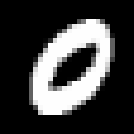
\includegraphics[interpolate=true,width=1.340000in,height=1.340000in]{dataset_samples-img0.png}}%
\end{pgfscope}%
\begin{pgfscope}%
\pgfpathrectangle{\pgfqpoint{1.516667in}{5.477218in}}{\pgfqpoint{1.333333in}{1.333333in}}%
\pgfusepath{clip}%
\pgfsys@transformshift{1.516667in}{5.477218in}%
\pgftext[left,bottom]{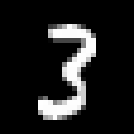
\includegraphics[interpolate=true,width=1.340000in,height=1.340000in]{dataset_samples-img1.png}}%
\end{pgfscope}%
\begin{pgfscope}%
\pgfpathrectangle{\pgfqpoint{0.050000in}{3.982228in}}{\pgfqpoint{1.333333in}{1.333333in}}%
\pgfusepath{clip}%
\pgfsys@transformshift{0.050000in}{3.982228in}%
\pgftext[left,bottom]{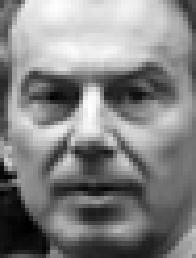
\includegraphics[interpolate=true,width=1.340000in,height=1.340000in]{dataset_samples-img2.png}}%
\end{pgfscope}%
\begin{pgfscope}%
\pgfpathrectangle{\pgfqpoint{1.516667in}{3.982228in}}{\pgfqpoint{1.333333in}{1.333333in}}%
\pgfusepath{clip}%
\pgfsys@transformshift{1.516667in}{3.982228in}%
\pgftext[left,bottom]{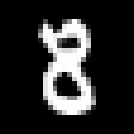
\includegraphics[interpolate=true,width=1.340000in,height=1.340000in]{dataset_samples-img3.png}}%
\end{pgfscope}%
\begin{pgfscope}%
\definecolor{textcolor}{rgb}{0.000000,0.000000,0.000000}%
\pgfsetstrokecolor{textcolor}%
\pgfsetfillcolor{textcolor}%
\pgftext[x=1.509000in,y=3.683890in,,base]{\color{textcolor}\rmfamily\fontsize{10.000000}{12.000000}\selectfont (a)}%
\end{pgfscope}%
\begin{pgfscope}%
\pgfsetbuttcap%
\pgfsetmiterjoin%
\definecolor{currentfill}{rgb}{1.000000,1.000000,1.000000}%
\pgfsetfillcolor{currentfill}%
\pgfsetlinewidth{0.000000pt}%
\definecolor{currentstroke}{rgb}{1.000000,1.000000,1.000000}%
\pgfsetstrokecolor{currentstroke}%
\pgfsetdash{}{0pt}%
\pgfpathmoveto{\pgfqpoint{-0.025000in}{0.008890in}}%
\pgfpathlineto{\pgfqpoint{2.925000in}{0.008890in}}%
\pgfpathlineto{\pgfqpoint{2.925000in}{3.508890in}}%
\pgfpathlineto{\pgfqpoint{-0.025000in}{3.508890in}}%
\pgfpathlineto{\pgfqpoint{-0.025000in}{0.008890in}}%
\pgfpathclose%
\pgfusepath{fill}%
\end{pgfscope}%
\begin{pgfscope}%
\pgfpathrectangle{\pgfqpoint{0.117792in}{1.853880in}}{\pgfqpoint{1.197749in}{1.580009in}}%
\pgfusepath{clip}%
\pgfsys@transformshift{0.117792in}{1.853880in}%
\pgftext[left,bottom]{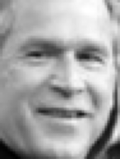
\includegraphics[interpolate=true,width=1.200000in,height=1.590000in]{dataset_samples-img4.png}}%
\end{pgfscope}%
\begin{pgfscope}%
\pgfpathrectangle{\pgfqpoint{1.584459in}{1.853880in}}{\pgfqpoint{1.197749in}{1.580009in}}%
\pgfusepath{clip}%
\pgfsys@transformshift{1.584459in}{1.853880in}%
\pgftext[left,bottom]{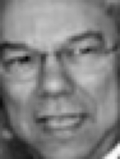
\includegraphics[interpolate=true,width=1.200000in,height=1.590000in]{dataset_samples-img5.png}}%
\end{pgfscope}%
\begin{pgfscope}%
\pgfpathrectangle{\pgfqpoint{0.117792in}{0.358890in}}{\pgfqpoint{1.197749in}{1.580009in}}%
\pgfusepath{clip}%
\pgfsys@transformshift{0.117792in}{0.358890in}%
\pgftext[left,bottom]{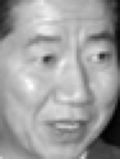
\includegraphics[interpolate=true,width=1.200000in,height=1.590000in]{dataset_samples-img6.png}}%
\end{pgfscope}%
\begin{pgfscope}%
\pgfpathrectangle{\pgfqpoint{1.584459in}{0.358890in}}{\pgfqpoint{1.197749in}{1.580009in}}%
\pgfusepath{clip}%
\pgfsys@transformshift{1.584459in}{0.358890in}%
\pgftext[left,bottom]{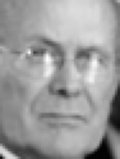
\includegraphics[interpolate=true,width=1.200000in,height=1.590000in]{dataset_samples-img7.png}}%
\end{pgfscope}%
\begin{pgfscope}%
\definecolor{textcolor}{rgb}{0.000000,0.000000,0.000000}%
\pgfsetstrokecolor{textcolor}%
\pgfsetfillcolor{textcolor}%
\pgftext[x=1.509000in,y=0.078890in,,base]{\color{textcolor}\rmfamily\fontsize{10.000000}{12.000000}\selectfont (c)}%
\end{pgfscope}%
\begin{pgfscope}%
\pgfsetbuttcap%
\pgfsetmiterjoin%
\definecolor{currentfill}{rgb}{1.000000,1.000000,1.000000}%
\pgfsetfillcolor{currentfill}%
\pgfsetlinewidth{0.000000pt}%
\definecolor{currentstroke}{rgb}{1.000000,1.000000,1.000000}%
\pgfsetstrokecolor{currentstroke}%
\pgfsetdash{}{0pt}%
\pgfpathmoveto{\pgfqpoint{2.925000in}{3.508890in}}%
\pgfpathlineto{\pgfqpoint{5.875000in}{3.508890in}}%
\pgfpathlineto{\pgfqpoint{5.875000in}{7.008890in}}%
\pgfpathlineto{\pgfqpoint{2.925000in}{7.008890in}}%
\pgfpathlineto{\pgfqpoint{2.925000in}{3.508890in}}%
\pgfpathclose%
\pgfusepath{fill}%
\end{pgfscope}%
\begin{pgfscope}%
\pgfpathrectangle{\pgfqpoint{3.000000in}{5.477218in}}{\pgfqpoint{1.333333in}{1.333333in}}%
\pgfusepath{clip}%
\pgfsys@transformshift{3.000000in}{5.477218in}%
\pgftext[left,bottom]{
\includegraphics[interpolate=true,width=1.340000in,height=1.340000in]{dataset_samples-img8.png}}%
\end{pgfscope}%
\begin{pgfscope}%
\pgfpathrectangle{\pgfqpoint{4.466667in}{5.477218in}}{\pgfqpoint{1.333333in}{1.333333in}}%
\pgfusepath{clip}%
\pgfsys@transformshift{4.466667in}{5.477218in}%
\pgftext[left,bottom]{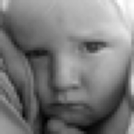
\includegraphics[interpolate=true,width=1.340000in,height=1.340000in]{dataset_samples-img9.png}}%
\end{pgfscope}%
\begin{pgfscope}%
\pgfpathrectangle{\pgfqpoint{3.000000in}{3.982228in}}{\pgfqpoint{1.333333in}{1.333333in}}%
\pgfusepath{clip}%
\pgfsys@transformshift{3.000000in}{3.982228in}%
\pgftext[left,bottom]{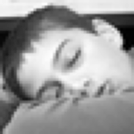
\includegraphics[interpolate=true,width=1.340000in,height=1.340000in]{dataset_samples-img10.png}}%
\end{pgfscope}%
\begin{pgfscope}%
\pgfpathrectangle{\pgfqpoint{4.466667in}{3.982228in}}{\pgfqpoint{1.333333in}{1.333333in}}%
\pgfusepath{clip}%
\pgfsys@transformshift{4.466667in}{3.982228in}%
\pgftext[left,bottom]{
\includegraphics[interpolate=true,width=1.340000in,height=1.340000in]{dataset_samples-img11.png}}%
\end{pgfscope}%
\begin{pgfscope}%
\definecolor{textcolor}{rgb}{0.000000,0.000000,0.000000}%
\pgfsetstrokecolor{textcolor}%
\pgfsetfillcolor{textcolor}%
\pgftext[x=4.459000in,y=3.683890in,,base]{\color{textcolor}\rmfamily\fontsize{10.000000}{12.000000}\selectfont (b)}%
\end{pgfscope}%
\begin{pgfscope}%
\pgfsetbuttcap%
\pgfsetmiterjoin%
\definecolor{currentfill}{rgb}{1.000000,1.000000,1.000000}%
\pgfsetfillcolor{currentfill}%
\pgfsetlinewidth{0.000000pt}%
\definecolor{currentstroke}{rgb}{1.000000,1.000000,1.000000}%
\pgfsetstrokecolor{currentstroke}%
\pgfsetdash{}{0pt}%
\pgfpathmoveto{\pgfqpoint{2.925000in}{0.008890in}}%
\pgfpathlineto{\pgfqpoint{5.875000in}{0.008890in}}%
\pgfpathlineto{\pgfqpoint{5.875000in}{3.508890in}}%
\pgfpathlineto{\pgfqpoint{2.925000in}{3.508890in}}%
\pgfpathlineto{\pgfqpoint{2.925000in}{0.008890in}}%
\pgfpathclose%
\pgfusepath{fill}%
\end{pgfscope}%
\begin{pgfscope}%
\pgfpathrectangle{\pgfqpoint{3.000000in}{1.977218in}}{\pgfqpoint{1.333333in}{1.333333in}}%
\pgfusepath{clip}%
\pgfsys@transformshift{3.000000in}{1.977218in}%
\pgftext[left,bottom]{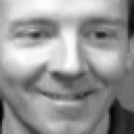
\includegraphics[interpolate=true,width=1.340000in,height=1.340000in]{dataset_samples-img12.png}}%
\end{pgfscope}%
\begin{pgfscope}%
\pgfpathrectangle{\pgfqpoint{4.466667in}{1.977218in}}{\pgfqpoint{1.333333in}{1.333333in}}%
\pgfusepath{clip}%
\pgfsys@transformshift{4.466667in}{1.977218in}%
\pgftext[left,bottom]{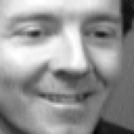
\includegraphics[interpolate=true,width=1.340000in,height=1.340000in]{dataset_samples-img13.png}}%
\end{pgfscope}%
\begin{pgfscope}%
\pgfpathrectangle{\pgfqpoint{3.000000in}{0.482228in}}{\pgfqpoint{1.333333in}{1.333333in}}%
\pgfusepath{clip}%
\pgfsys@transformshift{3.000000in}{0.482228in}%
\pgftext[left,bottom]{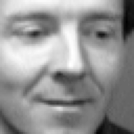
\includegraphics[interpolate=true,width=1.340000in,height=1.340000in]{dataset_samples-img14.png}}%
\end{pgfscope}%
\begin{pgfscope}%
\pgfpathrectangle{\pgfqpoint{4.466667in}{0.482228in}}{\pgfqpoint{1.333333in}{1.333333in}}%
\pgfusepath{clip}%
\pgfsys@transformshift{4.466667in}{0.482228in}%
\pgftext[left,bottom]{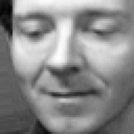
\includegraphics[interpolate=true,width=1.340000in,height=1.340000in]{dataset_samples-img15.png}}%
\end{pgfscope}%
\begin{pgfscope}%
\definecolor{textcolor}{rgb}{0.000000,0.000000,0.000000}%
\pgfsetstrokecolor{textcolor}%
\pgfsetfillcolor{textcolor}%
\pgftext[x=4.459000in,y=0.078890in,,base]{\color{textcolor}\rmfamily\fontsize{10.000000}{12.000000}\selectfont (d)}%
\end{pgfscope}%
\end{pgfpicture}%
\makeatother%
\endgroup%

	\end{center}
	\caption[Beispielbilder der natürlichen Datensätze]{Zu sehen sind je vier Beispielbilder der natürlichen Bilddatensätze aus dem Vergleich. \captiona Handgeschriebene Zahlen aus dem MNIST-Datensatz \captionb Beispielbilder aus dem FER-Datensatz \captionc Beispielbilder aus dem LFW-Datensatz \captiond Der Olivetti Faces Datensatz }
	\label{fig:Dataset_samples}
\end{figure}

Letztlich enthält der ICMR-Datensatz Genausprägungen von 801 Personen, die mit fünf
unterschiedlichen Arten von Krebs diagnostiziert wurden. Der Datensatz enthält Genausprägungen von
über 20 000 Genen, womit dieser Datensatz die höchste extrinsische Dimension im Vergleich besitzt.
In Tabelle \ref{tab:uebersicht-datensaetze} sind die extrinsischen und intrinsischen Dimensionen,
sowie die Stichprobengröße der Datensätze zusammengefasst. Die intrinsischen Dimensionen sind die
Schätzungen des in \subsecref{ch:Vergleich:sec:Methodik:subsec:SchaetzenDerIntrinsischenDim}
erläuterten Maximum Likelihood Schätzers für den jeweiligen Datensatz.

\begin{table}[]
	\centering
	\begin{tabular}{@{}lrrr@{}}
		\toprule
		Datensatz      & extrinsische Dimension $D$ & intrinsische Dimension $d$ & Stichprobengröße $n$ \\ \midrule
		Swiss Roll     & 3                          & 2                          & 5000                 \\
		Twin Peaks     & 3                          & 2                          & 5000                 \\
		MNIST          & 784                        & 10                         & 60 000               \\
		Olivetti Faces & 4096                       & 10                         & 400                  \\
		LFW            & 2914                       & 21                         & 2370                 \\
		FER            & 2304                       & 26                         & 28 709               \\
		ICMR           & 20 531                     & 22                         & 801                  \\
		\bottomrule
	\end{tabular}
	\caption{Übersicht über die extrinsischen und intrinsischen Dimensionen, sowie die Stichprobengröße der in diesem Vergleich verwendeten Datensätze. Bei Bilddatensätzen entspricht die extrinsische Dimension der Anzahl der Pixel im Bild. Die intrinsische Dimension wurde mit dem Maximum Likelihood Schätzer aus \subsecref{ch:Vergleich:sec:Methodik:subsec:SchaetzenDerIntrinsischenDim} mit einer Nachbarschaftsgröße $K=5$ geschätzt.}
	\label{tab:uebersicht-datensaetze}
\end{table}

\section{Parameterwahl und Trainingsdetails}
\label{ch:Vergleich:sec:ParameterwahlTrainingsdetails}

In diesem Abschnitt werden die gewählten (Hyper-)Parameter und Details des Trainierens der
Dimensionsreduktionsmethoden vorgestellt. Eine Übersicht ist in
Tabelle~\ref{tab:uebersicht-parameter} zu finden. Für die Hauptkomponentenanalyse gibt es neben der
Anzahl der zu behaltenden Hauptkomponenten keine Parameter. Die Anzahl der Hauptkomponenten
entspricht der intrinsischen Dimension, welche vom Datensatz abhängt und für alle Methoden
identisch ist. Dies trifft analog auf Kernel PCA und auf Locally Linear Embedding zu. Für
Autoencoder bestimmt die intrinsische Dimension die Größe der Bottleneck-Schicht. Für Kernel PCA
wird ein RBF-Kernel (Gauß-Kernel) eingesetzt, wofür ein Hyperparameter $\gamma$ gewählt werden
kann. Dieser wird Datensatz-spezifisch auf $\gamma = \sfrac{1}{D}$ gesetzt. Für Locally Linear
Embedding gibt es mehrere Parameter: (1) einen Parameter $K$, der die Größe der verwendeten
Nachbarschaft kontrolliert und (2) eine Regularisierungs-Konstante $\epsilon$, die auf die
Diagonale der lokalen Kovarianzmatrix addiert wird.

Den statistischen Methoden gegenüber haben Autoencoder deutlich mehr Freiheitsgrade, um die
Architektur zu bestimmen. Die wichtigsten Parameter sind die Anzahl der Schichten $m$, sowie die
Anzahl an Neuronen pro Schicht und die Wahl der Aktivierungsfunktionen. Daneben gibt es noch viele
weitere Freiheitsgrade für das Trainieren des Autoencoders, welche teilweise vom Datensatz
abhängen. Diese wurden für alle Autoencoder nahezu identisch gewählt und werden in
Appendix~\ref{ch:Appendix:Architektur-Details} genauer erläutert. Für beide künstlichen Datensätze
und für den Olivetti Face Datensatz wird ein dreischichtiger Autoencoder eingesetzt. Für alle
anderen Datensätze wird ein fünfschichtiger Autoencoder trainiert. Alle vollvernetzten Autoencoder
und der Contractive Autoencoder verwenden Sigmoid-Aktivierungsfunktionen im Encoder und Decoder.
Auf Bilddatensätzen wurden zusätzlich Convolutional Autoencoder trainiert, deren Architekturen an
\textcite[14]{Ghosh.2019} angelehnt sind und ebenfalls in
Appendix~\ref{ch:Appendix:Architektur-Details} spezifiziert sind.

\begin{table}[ht]
	\tymax=300pt
	\centering
	\begin{tabulary}{\linewidth}{CC}
		\toprule
		Methode                            & Parameter                                                            \\ \midrule
		Hauptkomponentenanalyse (PCA)      & --                                                                   \\ \midrule
		Kernel PCA                         & $\kappa(\vect{x}_1, \vect{x}_2) = \exp(- \norm{\vect{x}_1 - \vect{x}_2}^2/(2\gamma^2))$, $\gamma=\sfrac{1}{D}$ \\ \midrule
		Locally Linear Embedding (LLE)     & $K=10$, $\epsilon=1\mathrm{e}{-3}$                                   \\ \midrule
		Autoencoder (AE)                   & $m \in \{3, 5\}$, Sigmoid-Aktivierungsfunktion \newline (siehe
		Appendix~\ref{ch:Appendix:Architektur-Details})                                                           \\ \midrule Contractive Autoencoder (CAE) & $m = 3$, $\lambda=1\mathrm{e}{-4}$,
		Sigmoid-Aktivierungsfunktion (siehe Appendix~\ref{ch:Appendix:Architektur-Details})                       \\ \midrule
		Convolutional Autoencoder (ConvAE) & $m > 5$, ReLU-Aktivierungsfunktion \newline (siehe
		Appendix~\ref{ch:Appendix:Architektur-Details})                                                           \\ \bottomrule
	\end{tabulary}
	\caption[Übersicht über die verwendeten Parameter der Methoden]{Übersicht über die verwendeten Parameter. Hierbei ist $\kappa$ die Kernel-Funktion, $D$ die extrinsische Dimension des Datensatzes, $K$ die Nachbarschaftsgröße, $\epsilon$ eine Regularisierungskonstante für LLE, $m$ die Anzahl der Schichten im Autoencoder und $\lambda$ eine multiplikative Konstante für den kontrahierenden Fehlerterm des CAE.}
	\label{tab:uebersicht-parameter}
\end{table}
\section{Resultate}
\label{ch:Vergleich:sec:Resultate}

In diesem Abschnitt werden die Resultate des empirischen Vergleichs vorgestellt. Dazu werden die
Werte der verschiedenen Qualitätskriterien auf den künstlichen und natürlichen Datensätzen in
Abhängigkeit der Nachbarschaftsgröße $K$ abgebildet. Die verschiedenen Methoden wurden mit den im
vorhergehenden Abschnitt (\secref{ch:Vergleich:sec:ParameterwahlTrainingsdetails}) erläuterten
Parametern auf den künstlichen und natürlichen Datensätzen trainiert und hinsichtlich der in
\secref{ch:Vergleich:sec:Methodik:subsec:Qualitaetskriterien} vorgestellten Qualitätskriterien für
eine Nachbarschaftsgröße von $1 \leq K \leq 100$ evaluiert. Einige der Abbildungen für die
Qualitätskriterien sind im Appendix \ref{ch:Appendix:Qualitaetskriterien} zu finden.\unsure{vlt
	eine Tabelle mit Werten für K=10 (?) einfügen für die Übersicht?} In
\secref{ch:Vergleich:sec:Resultate:kuenstlich} werden die Ergebnisse auf den künstlichen
Datensätzen und in \secref{ch:Vergleich:sec:Resultate:natuerlich} die Ergebnisse auf den
natürlichen Datensätzen diskutiert. Letztlich wird in \secref{ch:Vergleich:sec:Resultate:PCA_AE}
der Zusammenhang zwischen der Hauptkomponentenanalyse und linearen Autoencodern empirisch
untersucht.

\subsection{Resultate auf künstlichen Datensätzen}
\label{ch:Vergleich:sec:Resultate:kuenstlich}

Die Qualitätskriterien für den Swiss Roll Datensatz sind in \figref{fig:SwissRollMetrics}
\begin{figure}[ht]
	\begin{center}
		%% Creator: Matplotlib, PGF backend
%%
%% To include the figure in your LaTeX document, write
%%   \input{<filename>.pgf}
%%
%% Make sure the required packages are loaded in your preamble
%%   \usepackage{pgf}
%%
%% Also ensure that all the required font packages are loaded; for instance,
%% the lmodern package is sometimes necessary when using math font.
%%   \usepackage{lmodern}
%%
%% Figures using additional raster images can only be included by \input if
%% they are in the same directory as the main LaTeX file. For loading figures
%% from other directories you can use the `import` package
%%   \usepackage{import}
%%
%% and then include the figures with
%%   \import{<path to file>}{<filename>.pgf}
%%
%% Matplotlib used the following preamble
%%   
%%   \usepackage{fontspec}
%%   \setmainfont{DejaVuSerif.ttf}[Path=\detokenize{/Users/moritzmistol/.pyenv/versions/3.9.13/envs/thesis/lib/python3.9/site-packages/matplotlib/mpl-data/fonts/ttf/}]
%%   \setsansfont{DejaVuSans.ttf}[Path=\detokenize{/Users/moritzmistol/.pyenv/versions/3.9.13/envs/thesis/lib/python3.9/site-packages/matplotlib/mpl-data/fonts/ttf/}]
%%   \setmonofont{DejaVuSansMono.ttf}[Path=\detokenize{/Users/moritzmistol/.pyenv/versions/3.9.13/envs/thesis/lib/python3.9/site-packages/matplotlib/mpl-data/fonts/ttf/}]
%%   \makeatletter\@ifpackageloaded{underscore}{}{\usepackage[strings]{underscore}}\makeatother
%%
\begingroup%
\makeatletter%
\begin{pgfpicture}%
\pgfpathrectangle{\pgfpointorigin}{\pgfqpoint{5.642256in}{4.634154in}}%
\pgfusepath{use as bounding box, clip}%
\begin{pgfscope}%
\pgfsetbuttcap%
\pgfsetmiterjoin%
\definecolor{currentfill}{rgb}{1.000000,1.000000,1.000000}%
\pgfsetfillcolor{currentfill}%
\pgfsetlinewidth{0.000000pt}%
\definecolor{currentstroke}{rgb}{1.000000,1.000000,1.000000}%
\pgfsetstrokecolor{currentstroke}%
\pgfsetdash{}{0pt}%
\pgfpathmoveto{\pgfqpoint{0.000000in}{-0.000000in}}%
\pgfpathlineto{\pgfqpoint{5.642256in}{-0.000000in}}%
\pgfpathlineto{\pgfqpoint{5.642256in}{4.634154in}}%
\pgfpathlineto{\pgfqpoint{0.000000in}{4.634154in}}%
\pgfpathlineto{\pgfqpoint{0.000000in}{-0.000000in}}%
\pgfpathclose%
\pgfusepath{fill}%
\end{pgfscope}%
\begin{pgfscope}%
\pgfsetbuttcap%
\pgfsetmiterjoin%
\definecolor{currentfill}{rgb}{1.000000,1.000000,1.000000}%
\pgfsetfillcolor{currentfill}%
\pgfsetlinewidth{0.000000pt}%
\definecolor{currentstroke}{rgb}{0.000000,0.000000,0.000000}%
\pgfsetstrokecolor{currentstroke}%
\pgfsetstrokeopacity{0.000000}%
\pgfsetdash{}{0pt}%
\pgfpathmoveto{\pgfqpoint{0.539970in}{2.747992in}}%
\pgfpathlineto{\pgfqpoint{2.781441in}{2.747992in}}%
\pgfpathlineto{\pgfqpoint{2.781441in}{4.374193in}}%
\pgfpathlineto{\pgfqpoint{0.539970in}{4.374193in}}%
\pgfpathlineto{\pgfqpoint{0.539970in}{2.747992in}}%
\pgfpathclose%
\pgfusepath{fill}%
\end{pgfscope}%
\begin{pgfscope}%
\pgfsetbuttcap%
\pgfsetroundjoin%
\definecolor{currentfill}{rgb}{0.000000,0.000000,0.000000}%
\pgfsetfillcolor{currentfill}%
\pgfsetlinewidth{0.501875pt}%
\definecolor{currentstroke}{rgb}{0.000000,0.000000,0.000000}%
\pgfsetstrokecolor{currentstroke}%
\pgfsetdash{}{0pt}%
\pgfsys@defobject{currentmarker}{\pgfqpoint{0.000000in}{0.000000in}}{\pgfqpoint{0.000000in}{0.041667in}}{%
\pgfpathmoveto{\pgfqpoint{0.000000in}{0.000000in}}%
\pgfpathlineto{\pgfqpoint{0.000000in}{0.041667in}}%
\pgfusepath{stroke,fill}%
}%
\begin{pgfscope}%
\pgfsys@transformshift{0.539970in}{2.747992in}%
\pgfsys@useobject{currentmarker}{}%
\end{pgfscope}%
\end{pgfscope}%
\begin{pgfscope}%
\pgfsetbuttcap%
\pgfsetroundjoin%
\definecolor{currentfill}{rgb}{0.000000,0.000000,0.000000}%
\pgfsetfillcolor{currentfill}%
\pgfsetlinewidth{0.501875pt}%
\definecolor{currentstroke}{rgb}{0.000000,0.000000,0.000000}%
\pgfsetstrokecolor{currentstroke}%
\pgfsetdash{}{0pt}%
\pgfsys@defobject{currentmarker}{\pgfqpoint{0.000000in}{-0.041667in}}{\pgfqpoint{0.000000in}{0.000000in}}{%
\pgfpathmoveto{\pgfqpoint{0.000000in}{0.000000in}}%
\pgfpathlineto{\pgfqpoint{0.000000in}{-0.041667in}}%
\pgfusepath{stroke,fill}%
}%
\begin{pgfscope}%
\pgfsys@transformshift{0.539970in}{4.374193in}%
\pgfsys@useobject{currentmarker}{}%
\end{pgfscope}%
\end{pgfscope}%
\begin{pgfscope}%
\definecolor{textcolor}{rgb}{0.000000,0.000000,0.000000}%
\pgfsetstrokecolor{textcolor}%
\pgfsetfillcolor{textcolor}%
\pgftext[x=0.539970in,y=2.699381in,,top]{\color{textcolor}\rmfamily\fontsize{10.000000}{12.000000}\selectfont \(\displaystyle {0}\)}%
\end{pgfscope}%
\begin{pgfscope}%
\pgfsetbuttcap%
\pgfsetroundjoin%
\definecolor{currentfill}{rgb}{0.000000,0.000000,0.000000}%
\pgfsetfillcolor{currentfill}%
\pgfsetlinewidth{0.501875pt}%
\definecolor{currentstroke}{rgb}{0.000000,0.000000,0.000000}%
\pgfsetstrokecolor{currentstroke}%
\pgfsetdash{}{0pt}%
\pgfsys@defobject{currentmarker}{\pgfqpoint{0.000000in}{0.000000in}}{\pgfqpoint{0.000000in}{0.041667in}}{%
\pgfpathmoveto{\pgfqpoint{0.000000in}{0.000000in}}%
\pgfpathlineto{\pgfqpoint{0.000000in}{0.041667in}}%
\pgfusepath{stroke,fill}%
}%
\begin{pgfscope}%
\pgfsys@transformshift{0.983826in}{2.747992in}%
\pgfsys@useobject{currentmarker}{}%
\end{pgfscope}%
\end{pgfscope}%
\begin{pgfscope}%
\pgfsetbuttcap%
\pgfsetroundjoin%
\definecolor{currentfill}{rgb}{0.000000,0.000000,0.000000}%
\pgfsetfillcolor{currentfill}%
\pgfsetlinewidth{0.501875pt}%
\definecolor{currentstroke}{rgb}{0.000000,0.000000,0.000000}%
\pgfsetstrokecolor{currentstroke}%
\pgfsetdash{}{0pt}%
\pgfsys@defobject{currentmarker}{\pgfqpoint{0.000000in}{-0.041667in}}{\pgfqpoint{0.000000in}{0.000000in}}{%
\pgfpathmoveto{\pgfqpoint{0.000000in}{0.000000in}}%
\pgfpathlineto{\pgfqpoint{0.000000in}{-0.041667in}}%
\pgfusepath{stroke,fill}%
}%
\begin{pgfscope}%
\pgfsys@transformshift{0.983826in}{4.374193in}%
\pgfsys@useobject{currentmarker}{}%
\end{pgfscope}%
\end{pgfscope}%
\begin{pgfscope}%
\definecolor{textcolor}{rgb}{0.000000,0.000000,0.000000}%
\pgfsetstrokecolor{textcolor}%
\pgfsetfillcolor{textcolor}%
\pgftext[x=0.983826in,y=2.699381in,,top]{\color{textcolor}\rmfamily\fontsize{10.000000}{12.000000}\selectfont \(\displaystyle {20}\)}%
\end{pgfscope}%
\begin{pgfscope}%
\pgfsetbuttcap%
\pgfsetroundjoin%
\definecolor{currentfill}{rgb}{0.000000,0.000000,0.000000}%
\pgfsetfillcolor{currentfill}%
\pgfsetlinewidth{0.501875pt}%
\definecolor{currentstroke}{rgb}{0.000000,0.000000,0.000000}%
\pgfsetstrokecolor{currentstroke}%
\pgfsetdash{}{0pt}%
\pgfsys@defobject{currentmarker}{\pgfqpoint{0.000000in}{0.000000in}}{\pgfqpoint{0.000000in}{0.041667in}}{%
\pgfpathmoveto{\pgfqpoint{0.000000in}{0.000000in}}%
\pgfpathlineto{\pgfqpoint{0.000000in}{0.041667in}}%
\pgfusepath{stroke,fill}%
}%
\begin{pgfscope}%
\pgfsys@transformshift{1.427681in}{2.747992in}%
\pgfsys@useobject{currentmarker}{}%
\end{pgfscope}%
\end{pgfscope}%
\begin{pgfscope}%
\pgfsetbuttcap%
\pgfsetroundjoin%
\definecolor{currentfill}{rgb}{0.000000,0.000000,0.000000}%
\pgfsetfillcolor{currentfill}%
\pgfsetlinewidth{0.501875pt}%
\definecolor{currentstroke}{rgb}{0.000000,0.000000,0.000000}%
\pgfsetstrokecolor{currentstroke}%
\pgfsetdash{}{0pt}%
\pgfsys@defobject{currentmarker}{\pgfqpoint{0.000000in}{-0.041667in}}{\pgfqpoint{0.000000in}{0.000000in}}{%
\pgfpathmoveto{\pgfqpoint{0.000000in}{0.000000in}}%
\pgfpathlineto{\pgfqpoint{0.000000in}{-0.041667in}}%
\pgfusepath{stroke,fill}%
}%
\begin{pgfscope}%
\pgfsys@transformshift{1.427681in}{4.374193in}%
\pgfsys@useobject{currentmarker}{}%
\end{pgfscope}%
\end{pgfscope}%
\begin{pgfscope}%
\definecolor{textcolor}{rgb}{0.000000,0.000000,0.000000}%
\pgfsetstrokecolor{textcolor}%
\pgfsetfillcolor{textcolor}%
\pgftext[x=1.427681in,y=2.699381in,,top]{\color{textcolor}\rmfamily\fontsize{10.000000}{12.000000}\selectfont \(\displaystyle {40}\)}%
\end{pgfscope}%
\begin{pgfscope}%
\pgfsetbuttcap%
\pgfsetroundjoin%
\definecolor{currentfill}{rgb}{0.000000,0.000000,0.000000}%
\pgfsetfillcolor{currentfill}%
\pgfsetlinewidth{0.501875pt}%
\definecolor{currentstroke}{rgb}{0.000000,0.000000,0.000000}%
\pgfsetstrokecolor{currentstroke}%
\pgfsetdash{}{0pt}%
\pgfsys@defobject{currentmarker}{\pgfqpoint{0.000000in}{0.000000in}}{\pgfqpoint{0.000000in}{0.041667in}}{%
\pgfpathmoveto{\pgfqpoint{0.000000in}{0.000000in}}%
\pgfpathlineto{\pgfqpoint{0.000000in}{0.041667in}}%
\pgfusepath{stroke,fill}%
}%
\begin{pgfscope}%
\pgfsys@transformshift{1.871537in}{2.747992in}%
\pgfsys@useobject{currentmarker}{}%
\end{pgfscope}%
\end{pgfscope}%
\begin{pgfscope}%
\pgfsetbuttcap%
\pgfsetroundjoin%
\definecolor{currentfill}{rgb}{0.000000,0.000000,0.000000}%
\pgfsetfillcolor{currentfill}%
\pgfsetlinewidth{0.501875pt}%
\definecolor{currentstroke}{rgb}{0.000000,0.000000,0.000000}%
\pgfsetstrokecolor{currentstroke}%
\pgfsetdash{}{0pt}%
\pgfsys@defobject{currentmarker}{\pgfqpoint{0.000000in}{-0.041667in}}{\pgfqpoint{0.000000in}{0.000000in}}{%
\pgfpathmoveto{\pgfqpoint{0.000000in}{0.000000in}}%
\pgfpathlineto{\pgfqpoint{0.000000in}{-0.041667in}}%
\pgfusepath{stroke,fill}%
}%
\begin{pgfscope}%
\pgfsys@transformshift{1.871537in}{4.374193in}%
\pgfsys@useobject{currentmarker}{}%
\end{pgfscope}%
\end{pgfscope}%
\begin{pgfscope}%
\definecolor{textcolor}{rgb}{0.000000,0.000000,0.000000}%
\pgfsetstrokecolor{textcolor}%
\pgfsetfillcolor{textcolor}%
\pgftext[x=1.871537in,y=2.699381in,,top]{\color{textcolor}\rmfamily\fontsize{10.000000}{12.000000}\selectfont \(\displaystyle {60}\)}%
\end{pgfscope}%
\begin{pgfscope}%
\pgfsetbuttcap%
\pgfsetroundjoin%
\definecolor{currentfill}{rgb}{0.000000,0.000000,0.000000}%
\pgfsetfillcolor{currentfill}%
\pgfsetlinewidth{0.501875pt}%
\definecolor{currentstroke}{rgb}{0.000000,0.000000,0.000000}%
\pgfsetstrokecolor{currentstroke}%
\pgfsetdash{}{0pt}%
\pgfsys@defobject{currentmarker}{\pgfqpoint{0.000000in}{0.000000in}}{\pgfqpoint{0.000000in}{0.041667in}}{%
\pgfpathmoveto{\pgfqpoint{0.000000in}{0.000000in}}%
\pgfpathlineto{\pgfqpoint{0.000000in}{0.041667in}}%
\pgfusepath{stroke,fill}%
}%
\begin{pgfscope}%
\pgfsys@transformshift{2.315393in}{2.747992in}%
\pgfsys@useobject{currentmarker}{}%
\end{pgfscope}%
\end{pgfscope}%
\begin{pgfscope}%
\pgfsetbuttcap%
\pgfsetroundjoin%
\definecolor{currentfill}{rgb}{0.000000,0.000000,0.000000}%
\pgfsetfillcolor{currentfill}%
\pgfsetlinewidth{0.501875pt}%
\definecolor{currentstroke}{rgb}{0.000000,0.000000,0.000000}%
\pgfsetstrokecolor{currentstroke}%
\pgfsetdash{}{0pt}%
\pgfsys@defobject{currentmarker}{\pgfqpoint{0.000000in}{-0.041667in}}{\pgfqpoint{0.000000in}{0.000000in}}{%
\pgfpathmoveto{\pgfqpoint{0.000000in}{0.000000in}}%
\pgfpathlineto{\pgfqpoint{0.000000in}{-0.041667in}}%
\pgfusepath{stroke,fill}%
}%
\begin{pgfscope}%
\pgfsys@transformshift{2.315393in}{4.374193in}%
\pgfsys@useobject{currentmarker}{}%
\end{pgfscope}%
\end{pgfscope}%
\begin{pgfscope}%
\definecolor{textcolor}{rgb}{0.000000,0.000000,0.000000}%
\pgfsetstrokecolor{textcolor}%
\pgfsetfillcolor{textcolor}%
\pgftext[x=2.315393in,y=2.699381in,,top]{\color{textcolor}\rmfamily\fontsize{10.000000}{12.000000}\selectfont \(\displaystyle {80}\)}%
\end{pgfscope}%
\begin{pgfscope}%
\pgfsetbuttcap%
\pgfsetroundjoin%
\definecolor{currentfill}{rgb}{0.000000,0.000000,0.000000}%
\pgfsetfillcolor{currentfill}%
\pgfsetlinewidth{0.501875pt}%
\definecolor{currentstroke}{rgb}{0.000000,0.000000,0.000000}%
\pgfsetstrokecolor{currentstroke}%
\pgfsetdash{}{0pt}%
\pgfsys@defobject{currentmarker}{\pgfqpoint{0.000000in}{0.000000in}}{\pgfqpoint{0.000000in}{0.020833in}}{%
\pgfpathmoveto{\pgfqpoint{0.000000in}{0.000000in}}%
\pgfpathlineto{\pgfqpoint{0.000000in}{0.020833in}}%
\pgfusepath{stroke,fill}%
}%
\begin{pgfscope}%
\pgfsys@transformshift{0.650934in}{2.747992in}%
\pgfsys@useobject{currentmarker}{}%
\end{pgfscope}%
\end{pgfscope}%
\begin{pgfscope}%
\pgfsetbuttcap%
\pgfsetroundjoin%
\definecolor{currentfill}{rgb}{0.000000,0.000000,0.000000}%
\pgfsetfillcolor{currentfill}%
\pgfsetlinewidth{0.501875pt}%
\definecolor{currentstroke}{rgb}{0.000000,0.000000,0.000000}%
\pgfsetstrokecolor{currentstroke}%
\pgfsetdash{}{0pt}%
\pgfsys@defobject{currentmarker}{\pgfqpoint{0.000000in}{-0.020833in}}{\pgfqpoint{0.000000in}{0.000000in}}{%
\pgfpathmoveto{\pgfqpoint{0.000000in}{0.000000in}}%
\pgfpathlineto{\pgfqpoint{0.000000in}{-0.020833in}}%
\pgfusepath{stroke,fill}%
}%
\begin{pgfscope}%
\pgfsys@transformshift{0.650934in}{4.374193in}%
\pgfsys@useobject{currentmarker}{}%
\end{pgfscope}%
\end{pgfscope}%
\begin{pgfscope}%
\pgfsetbuttcap%
\pgfsetroundjoin%
\definecolor{currentfill}{rgb}{0.000000,0.000000,0.000000}%
\pgfsetfillcolor{currentfill}%
\pgfsetlinewidth{0.501875pt}%
\definecolor{currentstroke}{rgb}{0.000000,0.000000,0.000000}%
\pgfsetstrokecolor{currentstroke}%
\pgfsetdash{}{0pt}%
\pgfsys@defobject{currentmarker}{\pgfqpoint{0.000000in}{0.000000in}}{\pgfqpoint{0.000000in}{0.020833in}}{%
\pgfpathmoveto{\pgfqpoint{0.000000in}{0.000000in}}%
\pgfpathlineto{\pgfqpoint{0.000000in}{0.020833in}}%
\pgfusepath{stroke,fill}%
}%
\begin{pgfscope}%
\pgfsys@transformshift{0.761898in}{2.747992in}%
\pgfsys@useobject{currentmarker}{}%
\end{pgfscope}%
\end{pgfscope}%
\begin{pgfscope}%
\pgfsetbuttcap%
\pgfsetroundjoin%
\definecolor{currentfill}{rgb}{0.000000,0.000000,0.000000}%
\pgfsetfillcolor{currentfill}%
\pgfsetlinewidth{0.501875pt}%
\definecolor{currentstroke}{rgb}{0.000000,0.000000,0.000000}%
\pgfsetstrokecolor{currentstroke}%
\pgfsetdash{}{0pt}%
\pgfsys@defobject{currentmarker}{\pgfqpoint{0.000000in}{-0.020833in}}{\pgfqpoint{0.000000in}{0.000000in}}{%
\pgfpathmoveto{\pgfqpoint{0.000000in}{0.000000in}}%
\pgfpathlineto{\pgfqpoint{0.000000in}{-0.020833in}}%
\pgfusepath{stroke,fill}%
}%
\begin{pgfscope}%
\pgfsys@transformshift{0.761898in}{4.374193in}%
\pgfsys@useobject{currentmarker}{}%
\end{pgfscope}%
\end{pgfscope}%
\begin{pgfscope}%
\pgfsetbuttcap%
\pgfsetroundjoin%
\definecolor{currentfill}{rgb}{0.000000,0.000000,0.000000}%
\pgfsetfillcolor{currentfill}%
\pgfsetlinewidth{0.501875pt}%
\definecolor{currentstroke}{rgb}{0.000000,0.000000,0.000000}%
\pgfsetstrokecolor{currentstroke}%
\pgfsetdash{}{0pt}%
\pgfsys@defobject{currentmarker}{\pgfqpoint{0.000000in}{0.000000in}}{\pgfqpoint{0.000000in}{0.020833in}}{%
\pgfpathmoveto{\pgfqpoint{0.000000in}{0.000000in}}%
\pgfpathlineto{\pgfqpoint{0.000000in}{0.020833in}}%
\pgfusepath{stroke,fill}%
}%
\begin{pgfscope}%
\pgfsys@transformshift{0.872862in}{2.747992in}%
\pgfsys@useobject{currentmarker}{}%
\end{pgfscope}%
\end{pgfscope}%
\begin{pgfscope}%
\pgfsetbuttcap%
\pgfsetroundjoin%
\definecolor{currentfill}{rgb}{0.000000,0.000000,0.000000}%
\pgfsetfillcolor{currentfill}%
\pgfsetlinewidth{0.501875pt}%
\definecolor{currentstroke}{rgb}{0.000000,0.000000,0.000000}%
\pgfsetstrokecolor{currentstroke}%
\pgfsetdash{}{0pt}%
\pgfsys@defobject{currentmarker}{\pgfqpoint{0.000000in}{-0.020833in}}{\pgfqpoint{0.000000in}{0.000000in}}{%
\pgfpathmoveto{\pgfqpoint{0.000000in}{0.000000in}}%
\pgfpathlineto{\pgfqpoint{0.000000in}{-0.020833in}}%
\pgfusepath{stroke,fill}%
}%
\begin{pgfscope}%
\pgfsys@transformshift{0.872862in}{4.374193in}%
\pgfsys@useobject{currentmarker}{}%
\end{pgfscope}%
\end{pgfscope}%
\begin{pgfscope}%
\pgfsetbuttcap%
\pgfsetroundjoin%
\definecolor{currentfill}{rgb}{0.000000,0.000000,0.000000}%
\pgfsetfillcolor{currentfill}%
\pgfsetlinewidth{0.501875pt}%
\definecolor{currentstroke}{rgb}{0.000000,0.000000,0.000000}%
\pgfsetstrokecolor{currentstroke}%
\pgfsetdash{}{0pt}%
\pgfsys@defobject{currentmarker}{\pgfqpoint{0.000000in}{0.000000in}}{\pgfqpoint{0.000000in}{0.020833in}}{%
\pgfpathmoveto{\pgfqpoint{0.000000in}{0.000000in}}%
\pgfpathlineto{\pgfqpoint{0.000000in}{0.020833in}}%
\pgfusepath{stroke,fill}%
}%
\begin{pgfscope}%
\pgfsys@transformshift{1.094790in}{2.747992in}%
\pgfsys@useobject{currentmarker}{}%
\end{pgfscope}%
\end{pgfscope}%
\begin{pgfscope}%
\pgfsetbuttcap%
\pgfsetroundjoin%
\definecolor{currentfill}{rgb}{0.000000,0.000000,0.000000}%
\pgfsetfillcolor{currentfill}%
\pgfsetlinewidth{0.501875pt}%
\definecolor{currentstroke}{rgb}{0.000000,0.000000,0.000000}%
\pgfsetstrokecolor{currentstroke}%
\pgfsetdash{}{0pt}%
\pgfsys@defobject{currentmarker}{\pgfqpoint{0.000000in}{-0.020833in}}{\pgfqpoint{0.000000in}{0.000000in}}{%
\pgfpathmoveto{\pgfqpoint{0.000000in}{0.000000in}}%
\pgfpathlineto{\pgfqpoint{0.000000in}{-0.020833in}}%
\pgfusepath{stroke,fill}%
}%
\begin{pgfscope}%
\pgfsys@transformshift{1.094790in}{4.374193in}%
\pgfsys@useobject{currentmarker}{}%
\end{pgfscope}%
\end{pgfscope}%
\begin{pgfscope}%
\pgfsetbuttcap%
\pgfsetroundjoin%
\definecolor{currentfill}{rgb}{0.000000,0.000000,0.000000}%
\pgfsetfillcolor{currentfill}%
\pgfsetlinewidth{0.501875pt}%
\definecolor{currentstroke}{rgb}{0.000000,0.000000,0.000000}%
\pgfsetstrokecolor{currentstroke}%
\pgfsetdash{}{0pt}%
\pgfsys@defobject{currentmarker}{\pgfqpoint{0.000000in}{0.000000in}}{\pgfqpoint{0.000000in}{0.020833in}}{%
\pgfpathmoveto{\pgfqpoint{0.000000in}{0.000000in}}%
\pgfpathlineto{\pgfqpoint{0.000000in}{0.020833in}}%
\pgfusepath{stroke,fill}%
}%
\begin{pgfscope}%
\pgfsys@transformshift{1.205753in}{2.747992in}%
\pgfsys@useobject{currentmarker}{}%
\end{pgfscope}%
\end{pgfscope}%
\begin{pgfscope}%
\pgfsetbuttcap%
\pgfsetroundjoin%
\definecolor{currentfill}{rgb}{0.000000,0.000000,0.000000}%
\pgfsetfillcolor{currentfill}%
\pgfsetlinewidth{0.501875pt}%
\definecolor{currentstroke}{rgb}{0.000000,0.000000,0.000000}%
\pgfsetstrokecolor{currentstroke}%
\pgfsetdash{}{0pt}%
\pgfsys@defobject{currentmarker}{\pgfqpoint{0.000000in}{-0.020833in}}{\pgfqpoint{0.000000in}{0.000000in}}{%
\pgfpathmoveto{\pgfqpoint{0.000000in}{0.000000in}}%
\pgfpathlineto{\pgfqpoint{0.000000in}{-0.020833in}}%
\pgfusepath{stroke,fill}%
}%
\begin{pgfscope}%
\pgfsys@transformshift{1.205753in}{4.374193in}%
\pgfsys@useobject{currentmarker}{}%
\end{pgfscope}%
\end{pgfscope}%
\begin{pgfscope}%
\pgfsetbuttcap%
\pgfsetroundjoin%
\definecolor{currentfill}{rgb}{0.000000,0.000000,0.000000}%
\pgfsetfillcolor{currentfill}%
\pgfsetlinewidth{0.501875pt}%
\definecolor{currentstroke}{rgb}{0.000000,0.000000,0.000000}%
\pgfsetstrokecolor{currentstroke}%
\pgfsetdash{}{0pt}%
\pgfsys@defobject{currentmarker}{\pgfqpoint{0.000000in}{0.000000in}}{\pgfqpoint{0.000000in}{0.020833in}}{%
\pgfpathmoveto{\pgfqpoint{0.000000in}{0.000000in}}%
\pgfpathlineto{\pgfqpoint{0.000000in}{0.020833in}}%
\pgfusepath{stroke,fill}%
}%
\begin{pgfscope}%
\pgfsys@transformshift{1.316717in}{2.747992in}%
\pgfsys@useobject{currentmarker}{}%
\end{pgfscope}%
\end{pgfscope}%
\begin{pgfscope}%
\pgfsetbuttcap%
\pgfsetroundjoin%
\definecolor{currentfill}{rgb}{0.000000,0.000000,0.000000}%
\pgfsetfillcolor{currentfill}%
\pgfsetlinewidth{0.501875pt}%
\definecolor{currentstroke}{rgb}{0.000000,0.000000,0.000000}%
\pgfsetstrokecolor{currentstroke}%
\pgfsetdash{}{0pt}%
\pgfsys@defobject{currentmarker}{\pgfqpoint{0.000000in}{-0.020833in}}{\pgfqpoint{0.000000in}{0.000000in}}{%
\pgfpathmoveto{\pgfqpoint{0.000000in}{0.000000in}}%
\pgfpathlineto{\pgfqpoint{0.000000in}{-0.020833in}}%
\pgfusepath{stroke,fill}%
}%
\begin{pgfscope}%
\pgfsys@transformshift{1.316717in}{4.374193in}%
\pgfsys@useobject{currentmarker}{}%
\end{pgfscope}%
\end{pgfscope}%
\begin{pgfscope}%
\pgfsetbuttcap%
\pgfsetroundjoin%
\definecolor{currentfill}{rgb}{0.000000,0.000000,0.000000}%
\pgfsetfillcolor{currentfill}%
\pgfsetlinewidth{0.501875pt}%
\definecolor{currentstroke}{rgb}{0.000000,0.000000,0.000000}%
\pgfsetstrokecolor{currentstroke}%
\pgfsetdash{}{0pt}%
\pgfsys@defobject{currentmarker}{\pgfqpoint{0.000000in}{0.000000in}}{\pgfqpoint{0.000000in}{0.020833in}}{%
\pgfpathmoveto{\pgfqpoint{0.000000in}{0.000000in}}%
\pgfpathlineto{\pgfqpoint{0.000000in}{0.020833in}}%
\pgfusepath{stroke,fill}%
}%
\begin{pgfscope}%
\pgfsys@transformshift{1.538645in}{2.747992in}%
\pgfsys@useobject{currentmarker}{}%
\end{pgfscope}%
\end{pgfscope}%
\begin{pgfscope}%
\pgfsetbuttcap%
\pgfsetroundjoin%
\definecolor{currentfill}{rgb}{0.000000,0.000000,0.000000}%
\pgfsetfillcolor{currentfill}%
\pgfsetlinewidth{0.501875pt}%
\definecolor{currentstroke}{rgb}{0.000000,0.000000,0.000000}%
\pgfsetstrokecolor{currentstroke}%
\pgfsetdash{}{0pt}%
\pgfsys@defobject{currentmarker}{\pgfqpoint{0.000000in}{-0.020833in}}{\pgfqpoint{0.000000in}{0.000000in}}{%
\pgfpathmoveto{\pgfqpoint{0.000000in}{0.000000in}}%
\pgfpathlineto{\pgfqpoint{0.000000in}{-0.020833in}}%
\pgfusepath{stroke,fill}%
}%
\begin{pgfscope}%
\pgfsys@transformshift{1.538645in}{4.374193in}%
\pgfsys@useobject{currentmarker}{}%
\end{pgfscope}%
\end{pgfscope}%
\begin{pgfscope}%
\pgfsetbuttcap%
\pgfsetroundjoin%
\definecolor{currentfill}{rgb}{0.000000,0.000000,0.000000}%
\pgfsetfillcolor{currentfill}%
\pgfsetlinewidth{0.501875pt}%
\definecolor{currentstroke}{rgb}{0.000000,0.000000,0.000000}%
\pgfsetstrokecolor{currentstroke}%
\pgfsetdash{}{0pt}%
\pgfsys@defobject{currentmarker}{\pgfqpoint{0.000000in}{0.000000in}}{\pgfqpoint{0.000000in}{0.020833in}}{%
\pgfpathmoveto{\pgfqpoint{0.000000in}{0.000000in}}%
\pgfpathlineto{\pgfqpoint{0.000000in}{0.020833in}}%
\pgfusepath{stroke,fill}%
}%
\begin{pgfscope}%
\pgfsys@transformshift{1.649609in}{2.747992in}%
\pgfsys@useobject{currentmarker}{}%
\end{pgfscope}%
\end{pgfscope}%
\begin{pgfscope}%
\pgfsetbuttcap%
\pgfsetroundjoin%
\definecolor{currentfill}{rgb}{0.000000,0.000000,0.000000}%
\pgfsetfillcolor{currentfill}%
\pgfsetlinewidth{0.501875pt}%
\definecolor{currentstroke}{rgb}{0.000000,0.000000,0.000000}%
\pgfsetstrokecolor{currentstroke}%
\pgfsetdash{}{0pt}%
\pgfsys@defobject{currentmarker}{\pgfqpoint{0.000000in}{-0.020833in}}{\pgfqpoint{0.000000in}{0.000000in}}{%
\pgfpathmoveto{\pgfqpoint{0.000000in}{0.000000in}}%
\pgfpathlineto{\pgfqpoint{0.000000in}{-0.020833in}}%
\pgfusepath{stroke,fill}%
}%
\begin{pgfscope}%
\pgfsys@transformshift{1.649609in}{4.374193in}%
\pgfsys@useobject{currentmarker}{}%
\end{pgfscope}%
\end{pgfscope}%
\begin{pgfscope}%
\pgfsetbuttcap%
\pgfsetroundjoin%
\definecolor{currentfill}{rgb}{0.000000,0.000000,0.000000}%
\pgfsetfillcolor{currentfill}%
\pgfsetlinewidth{0.501875pt}%
\definecolor{currentstroke}{rgb}{0.000000,0.000000,0.000000}%
\pgfsetstrokecolor{currentstroke}%
\pgfsetdash{}{0pt}%
\pgfsys@defobject{currentmarker}{\pgfqpoint{0.000000in}{0.000000in}}{\pgfqpoint{0.000000in}{0.020833in}}{%
\pgfpathmoveto{\pgfqpoint{0.000000in}{0.000000in}}%
\pgfpathlineto{\pgfqpoint{0.000000in}{0.020833in}}%
\pgfusepath{stroke,fill}%
}%
\begin{pgfscope}%
\pgfsys@transformshift{1.760573in}{2.747992in}%
\pgfsys@useobject{currentmarker}{}%
\end{pgfscope}%
\end{pgfscope}%
\begin{pgfscope}%
\pgfsetbuttcap%
\pgfsetroundjoin%
\definecolor{currentfill}{rgb}{0.000000,0.000000,0.000000}%
\pgfsetfillcolor{currentfill}%
\pgfsetlinewidth{0.501875pt}%
\definecolor{currentstroke}{rgb}{0.000000,0.000000,0.000000}%
\pgfsetstrokecolor{currentstroke}%
\pgfsetdash{}{0pt}%
\pgfsys@defobject{currentmarker}{\pgfqpoint{0.000000in}{-0.020833in}}{\pgfqpoint{0.000000in}{0.000000in}}{%
\pgfpathmoveto{\pgfqpoint{0.000000in}{0.000000in}}%
\pgfpathlineto{\pgfqpoint{0.000000in}{-0.020833in}}%
\pgfusepath{stroke,fill}%
}%
\begin{pgfscope}%
\pgfsys@transformshift{1.760573in}{4.374193in}%
\pgfsys@useobject{currentmarker}{}%
\end{pgfscope}%
\end{pgfscope}%
\begin{pgfscope}%
\pgfsetbuttcap%
\pgfsetroundjoin%
\definecolor{currentfill}{rgb}{0.000000,0.000000,0.000000}%
\pgfsetfillcolor{currentfill}%
\pgfsetlinewidth{0.501875pt}%
\definecolor{currentstroke}{rgb}{0.000000,0.000000,0.000000}%
\pgfsetstrokecolor{currentstroke}%
\pgfsetdash{}{0pt}%
\pgfsys@defobject{currentmarker}{\pgfqpoint{0.000000in}{0.000000in}}{\pgfqpoint{0.000000in}{0.020833in}}{%
\pgfpathmoveto{\pgfqpoint{0.000000in}{0.000000in}}%
\pgfpathlineto{\pgfqpoint{0.000000in}{0.020833in}}%
\pgfusepath{stroke,fill}%
}%
\begin{pgfscope}%
\pgfsys@transformshift{1.982501in}{2.747992in}%
\pgfsys@useobject{currentmarker}{}%
\end{pgfscope}%
\end{pgfscope}%
\begin{pgfscope}%
\pgfsetbuttcap%
\pgfsetroundjoin%
\definecolor{currentfill}{rgb}{0.000000,0.000000,0.000000}%
\pgfsetfillcolor{currentfill}%
\pgfsetlinewidth{0.501875pt}%
\definecolor{currentstroke}{rgb}{0.000000,0.000000,0.000000}%
\pgfsetstrokecolor{currentstroke}%
\pgfsetdash{}{0pt}%
\pgfsys@defobject{currentmarker}{\pgfqpoint{0.000000in}{-0.020833in}}{\pgfqpoint{0.000000in}{0.000000in}}{%
\pgfpathmoveto{\pgfqpoint{0.000000in}{0.000000in}}%
\pgfpathlineto{\pgfqpoint{0.000000in}{-0.020833in}}%
\pgfusepath{stroke,fill}%
}%
\begin{pgfscope}%
\pgfsys@transformshift{1.982501in}{4.374193in}%
\pgfsys@useobject{currentmarker}{}%
\end{pgfscope}%
\end{pgfscope}%
\begin{pgfscope}%
\pgfsetbuttcap%
\pgfsetroundjoin%
\definecolor{currentfill}{rgb}{0.000000,0.000000,0.000000}%
\pgfsetfillcolor{currentfill}%
\pgfsetlinewidth{0.501875pt}%
\definecolor{currentstroke}{rgb}{0.000000,0.000000,0.000000}%
\pgfsetstrokecolor{currentstroke}%
\pgfsetdash{}{0pt}%
\pgfsys@defobject{currentmarker}{\pgfqpoint{0.000000in}{0.000000in}}{\pgfqpoint{0.000000in}{0.020833in}}{%
\pgfpathmoveto{\pgfqpoint{0.000000in}{0.000000in}}%
\pgfpathlineto{\pgfqpoint{0.000000in}{0.020833in}}%
\pgfusepath{stroke,fill}%
}%
\begin{pgfscope}%
\pgfsys@transformshift{2.093465in}{2.747992in}%
\pgfsys@useobject{currentmarker}{}%
\end{pgfscope}%
\end{pgfscope}%
\begin{pgfscope}%
\pgfsetbuttcap%
\pgfsetroundjoin%
\definecolor{currentfill}{rgb}{0.000000,0.000000,0.000000}%
\pgfsetfillcolor{currentfill}%
\pgfsetlinewidth{0.501875pt}%
\definecolor{currentstroke}{rgb}{0.000000,0.000000,0.000000}%
\pgfsetstrokecolor{currentstroke}%
\pgfsetdash{}{0pt}%
\pgfsys@defobject{currentmarker}{\pgfqpoint{0.000000in}{-0.020833in}}{\pgfqpoint{0.000000in}{0.000000in}}{%
\pgfpathmoveto{\pgfqpoint{0.000000in}{0.000000in}}%
\pgfpathlineto{\pgfqpoint{0.000000in}{-0.020833in}}%
\pgfusepath{stroke,fill}%
}%
\begin{pgfscope}%
\pgfsys@transformshift{2.093465in}{4.374193in}%
\pgfsys@useobject{currentmarker}{}%
\end{pgfscope}%
\end{pgfscope}%
\begin{pgfscope}%
\pgfsetbuttcap%
\pgfsetroundjoin%
\definecolor{currentfill}{rgb}{0.000000,0.000000,0.000000}%
\pgfsetfillcolor{currentfill}%
\pgfsetlinewidth{0.501875pt}%
\definecolor{currentstroke}{rgb}{0.000000,0.000000,0.000000}%
\pgfsetstrokecolor{currentstroke}%
\pgfsetdash{}{0pt}%
\pgfsys@defobject{currentmarker}{\pgfqpoint{0.000000in}{0.000000in}}{\pgfqpoint{0.000000in}{0.020833in}}{%
\pgfpathmoveto{\pgfqpoint{0.000000in}{0.000000in}}%
\pgfpathlineto{\pgfqpoint{0.000000in}{0.020833in}}%
\pgfusepath{stroke,fill}%
}%
\begin{pgfscope}%
\pgfsys@transformshift{2.204429in}{2.747992in}%
\pgfsys@useobject{currentmarker}{}%
\end{pgfscope}%
\end{pgfscope}%
\begin{pgfscope}%
\pgfsetbuttcap%
\pgfsetroundjoin%
\definecolor{currentfill}{rgb}{0.000000,0.000000,0.000000}%
\pgfsetfillcolor{currentfill}%
\pgfsetlinewidth{0.501875pt}%
\definecolor{currentstroke}{rgb}{0.000000,0.000000,0.000000}%
\pgfsetstrokecolor{currentstroke}%
\pgfsetdash{}{0pt}%
\pgfsys@defobject{currentmarker}{\pgfqpoint{0.000000in}{-0.020833in}}{\pgfqpoint{0.000000in}{0.000000in}}{%
\pgfpathmoveto{\pgfqpoint{0.000000in}{0.000000in}}%
\pgfpathlineto{\pgfqpoint{0.000000in}{-0.020833in}}%
\pgfusepath{stroke,fill}%
}%
\begin{pgfscope}%
\pgfsys@transformshift{2.204429in}{4.374193in}%
\pgfsys@useobject{currentmarker}{}%
\end{pgfscope}%
\end{pgfscope}%
\begin{pgfscope}%
\pgfsetbuttcap%
\pgfsetroundjoin%
\definecolor{currentfill}{rgb}{0.000000,0.000000,0.000000}%
\pgfsetfillcolor{currentfill}%
\pgfsetlinewidth{0.501875pt}%
\definecolor{currentstroke}{rgb}{0.000000,0.000000,0.000000}%
\pgfsetstrokecolor{currentstroke}%
\pgfsetdash{}{0pt}%
\pgfsys@defobject{currentmarker}{\pgfqpoint{0.000000in}{0.000000in}}{\pgfqpoint{0.000000in}{0.020833in}}{%
\pgfpathmoveto{\pgfqpoint{0.000000in}{0.000000in}}%
\pgfpathlineto{\pgfqpoint{0.000000in}{0.020833in}}%
\pgfusepath{stroke,fill}%
}%
\begin{pgfscope}%
\pgfsys@transformshift{2.426357in}{2.747992in}%
\pgfsys@useobject{currentmarker}{}%
\end{pgfscope}%
\end{pgfscope}%
\begin{pgfscope}%
\pgfsetbuttcap%
\pgfsetroundjoin%
\definecolor{currentfill}{rgb}{0.000000,0.000000,0.000000}%
\pgfsetfillcolor{currentfill}%
\pgfsetlinewidth{0.501875pt}%
\definecolor{currentstroke}{rgb}{0.000000,0.000000,0.000000}%
\pgfsetstrokecolor{currentstroke}%
\pgfsetdash{}{0pt}%
\pgfsys@defobject{currentmarker}{\pgfqpoint{0.000000in}{-0.020833in}}{\pgfqpoint{0.000000in}{0.000000in}}{%
\pgfpathmoveto{\pgfqpoint{0.000000in}{0.000000in}}%
\pgfpathlineto{\pgfqpoint{0.000000in}{-0.020833in}}%
\pgfusepath{stroke,fill}%
}%
\begin{pgfscope}%
\pgfsys@transformshift{2.426357in}{4.374193in}%
\pgfsys@useobject{currentmarker}{}%
\end{pgfscope}%
\end{pgfscope}%
\begin{pgfscope}%
\pgfsetbuttcap%
\pgfsetroundjoin%
\definecolor{currentfill}{rgb}{0.000000,0.000000,0.000000}%
\pgfsetfillcolor{currentfill}%
\pgfsetlinewidth{0.501875pt}%
\definecolor{currentstroke}{rgb}{0.000000,0.000000,0.000000}%
\pgfsetstrokecolor{currentstroke}%
\pgfsetdash{}{0pt}%
\pgfsys@defobject{currentmarker}{\pgfqpoint{0.000000in}{0.000000in}}{\pgfqpoint{0.000000in}{0.020833in}}{%
\pgfpathmoveto{\pgfqpoint{0.000000in}{0.000000in}}%
\pgfpathlineto{\pgfqpoint{0.000000in}{0.020833in}}%
\pgfusepath{stroke,fill}%
}%
\begin{pgfscope}%
\pgfsys@transformshift{2.537321in}{2.747992in}%
\pgfsys@useobject{currentmarker}{}%
\end{pgfscope}%
\end{pgfscope}%
\begin{pgfscope}%
\pgfsetbuttcap%
\pgfsetroundjoin%
\definecolor{currentfill}{rgb}{0.000000,0.000000,0.000000}%
\pgfsetfillcolor{currentfill}%
\pgfsetlinewidth{0.501875pt}%
\definecolor{currentstroke}{rgb}{0.000000,0.000000,0.000000}%
\pgfsetstrokecolor{currentstroke}%
\pgfsetdash{}{0pt}%
\pgfsys@defobject{currentmarker}{\pgfqpoint{0.000000in}{-0.020833in}}{\pgfqpoint{0.000000in}{0.000000in}}{%
\pgfpathmoveto{\pgfqpoint{0.000000in}{0.000000in}}%
\pgfpathlineto{\pgfqpoint{0.000000in}{-0.020833in}}%
\pgfusepath{stroke,fill}%
}%
\begin{pgfscope}%
\pgfsys@transformshift{2.537321in}{4.374193in}%
\pgfsys@useobject{currentmarker}{}%
\end{pgfscope}%
\end{pgfscope}%
\begin{pgfscope}%
\pgfsetbuttcap%
\pgfsetroundjoin%
\definecolor{currentfill}{rgb}{0.000000,0.000000,0.000000}%
\pgfsetfillcolor{currentfill}%
\pgfsetlinewidth{0.501875pt}%
\definecolor{currentstroke}{rgb}{0.000000,0.000000,0.000000}%
\pgfsetstrokecolor{currentstroke}%
\pgfsetdash{}{0pt}%
\pgfsys@defobject{currentmarker}{\pgfqpoint{0.000000in}{0.000000in}}{\pgfqpoint{0.000000in}{0.020833in}}{%
\pgfpathmoveto{\pgfqpoint{0.000000in}{0.000000in}}%
\pgfpathlineto{\pgfqpoint{0.000000in}{0.020833in}}%
\pgfusepath{stroke,fill}%
}%
\begin{pgfscope}%
\pgfsys@transformshift{2.648285in}{2.747992in}%
\pgfsys@useobject{currentmarker}{}%
\end{pgfscope}%
\end{pgfscope}%
\begin{pgfscope}%
\pgfsetbuttcap%
\pgfsetroundjoin%
\definecolor{currentfill}{rgb}{0.000000,0.000000,0.000000}%
\pgfsetfillcolor{currentfill}%
\pgfsetlinewidth{0.501875pt}%
\definecolor{currentstroke}{rgb}{0.000000,0.000000,0.000000}%
\pgfsetstrokecolor{currentstroke}%
\pgfsetdash{}{0pt}%
\pgfsys@defobject{currentmarker}{\pgfqpoint{0.000000in}{-0.020833in}}{\pgfqpoint{0.000000in}{0.000000in}}{%
\pgfpathmoveto{\pgfqpoint{0.000000in}{0.000000in}}%
\pgfpathlineto{\pgfqpoint{0.000000in}{-0.020833in}}%
\pgfusepath{stroke,fill}%
}%
\begin{pgfscope}%
\pgfsys@transformshift{2.648285in}{4.374193in}%
\pgfsys@useobject{currentmarker}{}%
\end{pgfscope}%
\end{pgfscope}%
\begin{pgfscope}%
\pgfsetbuttcap%
\pgfsetroundjoin%
\definecolor{currentfill}{rgb}{0.000000,0.000000,0.000000}%
\pgfsetfillcolor{currentfill}%
\pgfsetlinewidth{0.501875pt}%
\definecolor{currentstroke}{rgb}{0.000000,0.000000,0.000000}%
\pgfsetstrokecolor{currentstroke}%
\pgfsetdash{}{0pt}%
\pgfsys@defobject{currentmarker}{\pgfqpoint{0.000000in}{0.000000in}}{\pgfqpoint{0.000000in}{0.020833in}}{%
\pgfpathmoveto{\pgfqpoint{0.000000in}{0.000000in}}%
\pgfpathlineto{\pgfqpoint{0.000000in}{0.020833in}}%
\pgfusepath{stroke,fill}%
}%
\begin{pgfscope}%
\pgfsys@transformshift{2.759249in}{2.747992in}%
\pgfsys@useobject{currentmarker}{}%
\end{pgfscope}%
\end{pgfscope}%
\begin{pgfscope}%
\pgfsetbuttcap%
\pgfsetroundjoin%
\definecolor{currentfill}{rgb}{0.000000,0.000000,0.000000}%
\pgfsetfillcolor{currentfill}%
\pgfsetlinewidth{0.501875pt}%
\definecolor{currentstroke}{rgb}{0.000000,0.000000,0.000000}%
\pgfsetstrokecolor{currentstroke}%
\pgfsetdash{}{0pt}%
\pgfsys@defobject{currentmarker}{\pgfqpoint{0.000000in}{-0.020833in}}{\pgfqpoint{0.000000in}{0.000000in}}{%
\pgfpathmoveto{\pgfqpoint{0.000000in}{0.000000in}}%
\pgfpathlineto{\pgfqpoint{0.000000in}{-0.020833in}}%
\pgfusepath{stroke,fill}%
}%
\begin{pgfscope}%
\pgfsys@transformshift{2.759249in}{4.374193in}%
\pgfsys@useobject{currentmarker}{}%
\end{pgfscope}%
\end{pgfscope}%
\begin{pgfscope}%
\definecolor{textcolor}{rgb}{0.000000,0.000000,0.000000}%
\pgfsetstrokecolor{textcolor}%
\pgfsetfillcolor{textcolor}%
\pgftext[x=1.660706in,y=2.509413in,,top]{\color{textcolor}\rmfamily\fontsize{10.000000}{12.000000}\selectfont \(\displaystyle K\)}%
\end{pgfscope}%
\begin{pgfscope}%
\pgfsetbuttcap%
\pgfsetroundjoin%
\definecolor{currentfill}{rgb}{0.000000,0.000000,0.000000}%
\pgfsetfillcolor{currentfill}%
\pgfsetlinewidth{0.501875pt}%
\definecolor{currentstroke}{rgb}{0.000000,0.000000,0.000000}%
\pgfsetstrokecolor{currentstroke}%
\pgfsetdash{}{0pt}%
\pgfsys@defobject{currentmarker}{\pgfqpoint{0.000000in}{0.000000in}}{\pgfqpoint{0.041667in}{0.000000in}}{%
\pgfpathmoveto{\pgfqpoint{0.000000in}{0.000000in}}%
\pgfpathlineto{\pgfqpoint{0.041667in}{0.000000in}}%
\pgfusepath{stroke,fill}%
}%
\begin{pgfscope}%
\pgfsys@transformshift{0.539970in}{2.892037in}%
\pgfsys@useobject{currentmarker}{}%
\end{pgfscope}%
\end{pgfscope}%
\begin{pgfscope}%
\pgfsetbuttcap%
\pgfsetroundjoin%
\definecolor{currentfill}{rgb}{0.000000,0.000000,0.000000}%
\pgfsetfillcolor{currentfill}%
\pgfsetlinewidth{0.501875pt}%
\definecolor{currentstroke}{rgb}{0.000000,0.000000,0.000000}%
\pgfsetstrokecolor{currentstroke}%
\pgfsetdash{}{0pt}%
\pgfsys@defobject{currentmarker}{\pgfqpoint{-0.041667in}{0.000000in}}{\pgfqpoint{-0.000000in}{0.000000in}}{%
\pgfpathmoveto{\pgfqpoint{-0.000000in}{0.000000in}}%
\pgfpathlineto{\pgfqpoint{-0.041667in}{0.000000in}}%
\pgfusepath{stroke,fill}%
}%
\begin{pgfscope}%
\pgfsys@transformshift{2.781441in}{2.892037in}%
\pgfsys@useobject{currentmarker}{}%
\end{pgfscope}%
\end{pgfscope}%
\begin{pgfscope}%
\definecolor{textcolor}{rgb}{0.000000,0.000000,0.000000}%
\pgfsetstrokecolor{textcolor}%
\pgfsetfillcolor{textcolor}%
\pgftext[x=0.244444in, y=2.839276in, left, base]{\color{textcolor}\rmfamily\fontsize{10.000000}{12.000000}\selectfont \(\displaystyle {0.82}\)}%
\end{pgfscope}%
\begin{pgfscope}%
\pgfsetbuttcap%
\pgfsetroundjoin%
\definecolor{currentfill}{rgb}{0.000000,0.000000,0.000000}%
\pgfsetfillcolor{currentfill}%
\pgfsetlinewidth{0.501875pt}%
\definecolor{currentstroke}{rgb}{0.000000,0.000000,0.000000}%
\pgfsetstrokecolor{currentstroke}%
\pgfsetdash{}{0pt}%
\pgfsys@defobject{currentmarker}{\pgfqpoint{0.000000in}{0.000000in}}{\pgfqpoint{0.041667in}{0.000000in}}{%
\pgfpathmoveto{\pgfqpoint{0.000000in}{0.000000in}}%
\pgfpathlineto{\pgfqpoint{0.041667in}{0.000000in}}%
\pgfusepath{stroke,fill}%
}%
\begin{pgfscope}%
\pgfsys@transformshift{0.539970in}{3.324531in}%
\pgfsys@useobject{currentmarker}{}%
\end{pgfscope}%
\end{pgfscope}%
\begin{pgfscope}%
\pgfsetbuttcap%
\pgfsetroundjoin%
\definecolor{currentfill}{rgb}{0.000000,0.000000,0.000000}%
\pgfsetfillcolor{currentfill}%
\pgfsetlinewidth{0.501875pt}%
\definecolor{currentstroke}{rgb}{0.000000,0.000000,0.000000}%
\pgfsetstrokecolor{currentstroke}%
\pgfsetdash{}{0pt}%
\pgfsys@defobject{currentmarker}{\pgfqpoint{-0.041667in}{0.000000in}}{\pgfqpoint{-0.000000in}{0.000000in}}{%
\pgfpathmoveto{\pgfqpoint{-0.000000in}{0.000000in}}%
\pgfpathlineto{\pgfqpoint{-0.041667in}{0.000000in}}%
\pgfusepath{stroke,fill}%
}%
\begin{pgfscope}%
\pgfsys@transformshift{2.781441in}{3.324531in}%
\pgfsys@useobject{currentmarker}{}%
\end{pgfscope}%
\end{pgfscope}%
\begin{pgfscope}%
\definecolor{textcolor}{rgb}{0.000000,0.000000,0.000000}%
\pgfsetstrokecolor{textcolor}%
\pgfsetfillcolor{textcolor}%
\pgftext[x=0.244444in, y=3.271770in, left, base]{\color{textcolor}\rmfamily\fontsize{10.000000}{12.000000}\selectfont \(\displaystyle {0.84}\)}%
\end{pgfscope}%
\begin{pgfscope}%
\pgfsetbuttcap%
\pgfsetroundjoin%
\definecolor{currentfill}{rgb}{0.000000,0.000000,0.000000}%
\pgfsetfillcolor{currentfill}%
\pgfsetlinewidth{0.501875pt}%
\definecolor{currentstroke}{rgb}{0.000000,0.000000,0.000000}%
\pgfsetstrokecolor{currentstroke}%
\pgfsetdash{}{0pt}%
\pgfsys@defobject{currentmarker}{\pgfqpoint{0.000000in}{0.000000in}}{\pgfqpoint{0.041667in}{0.000000in}}{%
\pgfpathmoveto{\pgfqpoint{0.000000in}{0.000000in}}%
\pgfpathlineto{\pgfqpoint{0.041667in}{0.000000in}}%
\pgfusepath{stroke,fill}%
}%
\begin{pgfscope}%
\pgfsys@transformshift{0.539970in}{3.757025in}%
\pgfsys@useobject{currentmarker}{}%
\end{pgfscope}%
\end{pgfscope}%
\begin{pgfscope}%
\pgfsetbuttcap%
\pgfsetroundjoin%
\definecolor{currentfill}{rgb}{0.000000,0.000000,0.000000}%
\pgfsetfillcolor{currentfill}%
\pgfsetlinewidth{0.501875pt}%
\definecolor{currentstroke}{rgb}{0.000000,0.000000,0.000000}%
\pgfsetstrokecolor{currentstroke}%
\pgfsetdash{}{0pt}%
\pgfsys@defobject{currentmarker}{\pgfqpoint{-0.041667in}{0.000000in}}{\pgfqpoint{-0.000000in}{0.000000in}}{%
\pgfpathmoveto{\pgfqpoint{-0.000000in}{0.000000in}}%
\pgfpathlineto{\pgfqpoint{-0.041667in}{0.000000in}}%
\pgfusepath{stroke,fill}%
}%
\begin{pgfscope}%
\pgfsys@transformshift{2.781441in}{3.757025in}%
\pgfsys@useobject{currentmarker}{}%
\end{pgfscope}%
\end{pgfscope}%
\begin{pgfscope}%
\definecolor{textcolor}{rgb}{0.000000,0.000000,0.000000}%
\pgfsetstrokecolor{textcolor}%
\pgfsetfillcolor{textcolor}%
\pgftext[x=0.244444in, y=3.704263in, left, base]{\color{textcolor}\rmfamily\fontsize{10.000000}{12.000000}\selectfont \(\displaystyle {0.86}\)}%
\end{pgfscope}%
\begin{pgfscope}%
\pgfsetbuttcap%
\pgfsetroundjoin%
\definecolor{currentfill}{rgb}{0.000000,0.000000,0.000000}%
\pgfsetfillcolor{currentfill}%
\pgfsetlinewidth{0.501875pt}%
\definecolor{currentstroke}{rgb}{0.000000,0.000000,0.000000}%
\pgfsetstrokecolor{currentstroke}%
\pgfsetdash{}{0pt}%
\pgfsys@defobject{currentmarker}{\pgfqpoint{0.000000in}{0.000000in}}{\pgfqpoint{0.041667in}{0.000000in}}{%
\pgfpathmoveto{\pgfqpoint{0.000000in}{0.000000in}}%
\pgfpathlineto{\pgfqpoint{0.041667in}{0.000000in}}%
\pgfusepath{stroke,fill}%
}%
\begin{pgfscope}%
\pgfsys@transformshift{0.539970in}{4.189519in}%
\pgfsys@useobject{currentmarker}{}%
\end{pgfscope}%
\end{pgfscope}%
\begin{pgfscope}%
\pgfsetbuttcap%
\pgfsetroundjoin%
\definecolor{currentfill}{rgb}{0.000000,0.000000,0.000000}%
\pgfsetfillcolor{currentfill}%
\pgfsetlinewidth{0.501875pt}%
\definecolor{currentstroke}{rgb}{0.000000,0.000000,0.000000}%
\pgfsetstrokecolor{currentstroke}%
\pgfsetdash{}{0pt}%
\pgfsys@defobject{currentmarker}{\pgfqpoint{-0.041667in}{0.000000in}}{\pgfqpoint{-0.000000in}{0.000000in}}{%
\pgfpathmoveto{\pgfqpoint{-0.000000in}{0.000000in}}%
\pgfpathlineto{\pgfqpoint{-0.041667in}{0.000000in}}%
\pgfusepath{stroke,fill}%
}%
\begin{pgfscope}%
\pgfsys@transformshift{2.781441in}{4.189519in}%
\pgfsys@useobject{currentmarker}{}%
\end{pgfscope}%
\end{pgfscope}%
\begin{pgfscope}%
\definecolor{textcolor}{rgb}{0.000000,0.000000,0.000000}%
\pgfsetstrokecolor{textcolor}%
\pgfsetfillcolor{textcolor}%
\pgftext[x=0.244444in, y=4.136757in, left, base]{\color{textcolor}\rmfamily\fontsize{10.000000}{12.000000}\selectfont \(\displaystyle {0.88}\)}%
\end{pgfscope}%
\begin{pgfscope}%
\pgfsetbuttcap%
\pgfsetroundjoin%
\definecolor{currentfill}{rgb}{0.000000,0.000000,0.000000}%
\pgfsetfillcolor{currentfill}%
\pgfsetlinewidth{0.501875pt}%
\definecolor{currentstroke}{rgb}{0.000000,0.000000,0.000000}%
\pgfsetstrokecolor{currentstroke}%
\pgfsetdash{}{0pt}%
\pgfsys@defobject{currentmarker}{\pgfqpoint{0.000000in}{0.000000in}}{\pgfqpoint{0.020833in}{0.000000in}}{%
\pgfpathmoveto{\pgfqpoint{0.000000in}{0.000000in}}%
\pgfpathlineto{\pgfqpoint{0.020833in}{0.000000in}}%
\pgfusepath{stroke,fill}%
}%
\begin{pgfscope}%
\pgfsys@transformshift{0.539970in}{2.783914in}%
\pgfsys@useobject{currentmarker}{}%
\end{pgfscope}%
\end{pgfscope}%
\begin{pgfscope}%
\pgfsetbuttcap%
\pgfsetroundjoin%
\definecolor{currentfill}{rgb}{0.000000,0.000000,0.000000}%
\pgfsetfillcolor{currentfill}%
\pgfsetlinewidth{0.501875pt}%
\definecolor{currentstroke}{rgb}{0.000000,0.000000,0.000000}%
\pgfsetstrokecolor{currentstroke}%
\pgfsetdash{}{0pt}%
\pgfsys@defobject{currentmarker}{\pgfqpoint{-0.020833in}{0.000000in}}{\pgfqpoint{-0.000000in}{0.000000in}}{%
\pgfpathmoveto{\pgfqpoint{-0.000000in}{0.000000in}}%
\pgfpathlineto{\pgfqpoint{-0.020833in}{0.000000in}}%
\pgfusepath{stroke,fill}%
}%
\begin{pgfscope}%
\pgfsys@transformshift{2.781441in}{2.783914in}%
\pgfsys@useobject{currentmarker}{}%
\end{pgfscope}%
\end{pgfscope}%
\begin{pgfscope}%
\pgfsetbuttcap%
\pgfsetroundjoin%
\definecolor{currentfill}{rgb}{0.000000,0.000000,0.000000}%
\pgfsetfillcolor{currentfill}%
\pgfsetlinewidth{0.501875pt}%
\definecolor{currentstroke}{rgb}{0.000000,0.000000,0.000000}%
\pgfsetstrokecolor{currentstroke}%
\pgfsetdash{}{0pt}%
\pgfsys@defobject{currentmarker}{\pgfqpoint{0.000000in}{0.000000in}}{\pgfqpoint{0.020833in}{0.000000in}}{%
\pgfpathmoveto{\pgfqpoint{0.000000in}{0.000000in}}%
\pgfpathlineto{\pgfqpoint{0.020833in}{0.000000in}}%
\pgfusepath{stroke,fill}%
}%
\begin{pgfscope}%
\pgfsys@transformshift{0.539970in}{3.000161in}%
\pgfsys@useobject{currentmarker}{}%
\end{pgfscope}%
\end{pgfscope}%
\begin{pgfscope}%
\pgfsetbuttcap%
\pgfsetroundjoin%
\definecolor{currentfill}{rgb}{0.000000,0.000000,0.000000}%
\pgfsetfillcolor{currentfill}%
\pgfsetlinewidth{0.501875pt}%
\definecolor{currentstroke}{rgb}{0.000000,0.000000,0.000000}%
\pgfsetstrokecolor{currentstroke}%
\pgfsetdash{}{0pt}%
\pgfsys@defobject{currentmarker}{\pgfqpoint{-0.020833in}{0.000000in}}{\pgfqpoint{-0.000000in}{0.000000in}}{%
\pgfpathmoveto{\pgfqpoint{-0.000000in}{0.000000in}}%
\pgfpathlineto{\pgfqpoint{-0.020833in}{0.000000in}}%
\pgfusepath{stroke,fill}%
}%
\begin{pgfscope}%
\pgfsys@transformshift{2.781441in}{3.000161in}%
\pgfsys@useobject{currentmarker}{}%
\end{pgfscope}%
\end{pgfscope}%
\begin{pgfscope}%
\pgfsetbuttcap%
\pgfsetroundjoin%
\definecolor{currentfill}{rgb}{0.000000,0.000000,0.000000}%
\pgfsetfillcolor{currentfill}%
\pgfsetlinewidth{0.501875pt}%
\definecolor{currentstroke}{rgb}{0.000000,0.000000,0.000000}%
\pgfsetstrokecolor{currentstroke}%
\pgfsetdash{}{0pt}%
\pgfsys@defobject{currentmarker}{\pgfqpoint{0.000000in}{0.000000in}}{\pgfqpoint{0.020833in}{0.000000in}}{%
\pgfpathmoveto{\pgfqpoint{0.000000in}{0.000000in}}%
\pgfpathlineto{\pgfqpoint{0.020833in}{0.000000in}}%
\pgfusepath{stroke,fill}%
}%
\begin{pgfscope}%
\pgfsys@transformshift{0.539970in}{3.108284in}%
\pgfsys@useobject{currentmarker}{}%
\end{pgfscope}%
\end{pgfscope}%
\begin{pgfscope}%
\pgfsetbuttcap%
\pgfsetroundjoin%
\definecolor{currentfill}{rgb}{0.000000,0.000000,0.000000}%
\pgfsetfillcolor{currentfill}%
\pgfsetlinewidth{0.501875pt}%
\definecolor{currentstroke}{rgb}{0.000000,0.000000,0.000000}%
\pgfsetstrokecolor{currentstroke}%
\pgfsetdash{}{0pt}%
\pgfsys@defobject{currentmarker}{\pgfqpoint{-0.020833in}{0.000000in}}{\pgfqpoint{-0.000000in}{0.000000in}}{%
\pgfpathmoveto{\pgfqpoint{-0.000000in}{0.000000in}}%
\pgfpathlineto{\pgfqpoint{-0.020833in}{0.000000in}}%
\pgfusepath{stroke,fill}%
}%
\begin{pgfscope}%
\pgfsys@transformshift{2.781441in}{3.108284in}%
\pgfsys@useobject{currentmarker}{}%
\end{pgfscope}%
\end{pgfscope}%
\begin{pgfscope}%
\pgfsetbuttcap%
\pgfsetroundjoin%
\definecolor{currentfill}{rgb}{0.000000,0.000000,0.000000}%
\pgfsetfillcolor{currentfill}%
\pgfsetlinewidth{0.501875pt}%
\definecolor{currentstroke}{rgb}{0.000000,0.000000,0.000000}%
\pgfsetstrokecolor{currentstroke}%
\pgfsetdash{}{0pt}%
\pgfsys@defobject{currentmarker}{\pgfqpoint{0.000000in}{0.000000in}}{\pgfqpoint{0.020833in}{0.000000in}}{%
\pgfpathmoveto{\pgfqpoint{0.000000in}{0.000000in}}%
\pgfpathlineto{\pgfqpoint{0.020833in}{0.000000in}}%
\pgfusepath{stroke,fill}%
}%
\begin{pgfscope}%
\pgfsys@transformshift{0.539970in}{3.216408in}%
\pgfsys@useobject{currentmarker}{}%
\end{pgfscope}%
\end{pgfscope}%
\begin{pgfscope}%
\pgfsetbuttcap%
\pgfsetroundjoin%
\definecolor{currentfill}{rgb}{0.000000,0.000000,0.000000}%
\pgfsetfillcolor{currentfill}%
\pgfsetlinewidth{0.501875pt}%
\definecolor{currentstroke}{rgb}{0.000000,0.000000,0.000000}%
\pgfsetstrokecolor{currentstroke}%
\pgfsetdash{}{0pt}%
\pgfsys@defobject{currentmarker}{\pgfqpoint{-0.020833in}{0.000000in}}{\pgfqpoint{-0.000000in}{0.000000in}}{%
\pgfpathmoveto{\pgfqpoint{-0.000000in}{0.000000in}}%
\pgfpathlineto{\pgfqpoint{-0.020833in}{0.000000in}}%
\pgfusepath{stroke,fill}%
}%
\begin{pgfscope}%
\pgfsys@transformshift{2.781441in}{3.216408in}%
\pgfsys@useobject{currentmarker}{}%
\end{pgfscope}%
\end{pgfscope}%
\begin{pgfscope}%
\pgfsetbuttcap%
\pgfsetroundjoin%
\definecolor{currentfill}{rgb}{0.000000,0.000000,0.000000}%
\pgfsetfillcolor{currentfill}%
\pgfsetlinewidth{0.501875pt}%
\definecolor{currentstroke}{rgb}{0.000000,0.000000,0.000000}%
\pgfsetstrokecolor{currentstroke}%
\pgfsetdash{}{0pt}%
\pgfsys@defobject{currentmarker}{\pgfqpoint{0.000000in}{0.000000in}}{\pgfqpoint{0.020833in}{0.000000in}}{%
\pgfpathmoveto{\pgfqpoint{0.000000in}{0.000000in}}%
\pgfpathlineto{\pgfqpoint{0.020833in}{0.000000in}}%
\pgfusepath{stroke,fill}%
}%
\begin{pgfscope}%
\pgfsys@transformshift{0.539970in}{3.432655in}%
\pgfsys@useobject{currentmarker}{}%
\end{pgfscope}%
\end{pgfscope}%
\begin{pgfscope}%
\pgfsetbuttcap%
\pgfsetroundjoin%
\definecolor{currentfill}{rgb}{0.000000,0.000000,0.000000}%
\pgfsetfillcolor{currentfill}%
\pgfsetlinewidth{0.501875pt}%
\definecolor{currentstroke}{rgb}{0.000000,0.000000,0.000000}%
\pgfsetstrokecolor{currentstroke}%
\pgfsetdash{}{0pt}%
\pgfsys@defobject{currentmarker}{\pgfqpoint{-0.020833in}{0.000000in}}{\pgfqpoint{-0.000000in}{0.000000in}}{%
\pgfpathmoveto{\pgfqpoint{-0.000000in}{0.000000in}}%
\pgfpathlineto{\pgfqpoint{-0.020833in}{0.000000in}}%
\pgfusepath{stroke,fill}%
}%
\begin{pgfscope}%
\pgfsys@transformshift{2.781441in}{3.432655in}%
\pgfsys@useobject{currentmarker}{}%
\end{pgfscope}%
\end{pgfscope}%
\begin{pgfscope}%
\pgfsetbuttcap%
\pgfsetroundjoin%
\definecolor{currentfill}{rgb}{0.000000,0.000000,0.000000}%
\pgfsetfillcolor{currentfill}%
\pgfsetlinewidth{0.501875pt}%
\definecolor{currentstroke}{rgb}{0.000000,0.000000,0.000000}%
\pgfsetstrokecolor{currentstroke}%
\pgfsetdash{}{0pt}%
\pgfsys@defobject{currentmarker}{\pgfqpoint{0.000000in}{0.000000in}}{\pgfqpoint{0.020833in}{0.000000in}}{%
\pgfpathmoveto{\pgfqpoint{0.000000in}{0.000000in}}%
\pgfpathlineto{\pgfqpoint{0.020833in}{0.000000in}}%
\pgfusepath{stroke,fill}%
}%
\begin{pgfscope}%
\pgfsys@transformshift{0.539970in}{3.540778in}%
\pgfsys@useobject{currentmarker}{}%
\end{pgfscope}%
\end{pgfscope}%
\begin{pgfscope}%
\pgfsetbuttcap%
\pgfsetroundjoin%
\definecolor{currentfill}{rgb}{0.000000,0.000000,0.000000}%
\pgfsetfillcolor{currentfill}%
\pgfsetlinewidth{0.501875pt}%
\definecolor{currentstroke}{rgb}{0.000000,0.000000,0.000000}%
\pgfsetstrokecolor{currentstroke}%
\pgfsetdash{}{0pt}%
\pgfsys@defobject{currentmarker}{\pgfqpoint{-0.020833in}{0.000000in}}{\pgfqpoint{-0.000000in}{0.000000in}}{%
\pgfpathmoveto{\pgfqpoint{-0.000000in}{0.000000in}}%
\pgfpathlineto{\pgfqpoint{-0.020833in}{0.000000in}}%
\pgfusepath{stroke,fill}%
}%
\begin{pgfscope}%
\pgfsys@transformshift{2.781441in}{3.540778in}%
\pgfsys@useobject{currentmarker}{}%
\end{pgfscope}%
\end{pgfscope}%
\begin{pgfscope}%
\pgfsetbuttcap%
\pgfsetroundjoin%
\definecolor{currentfill}{rgb}{0.000000,0.000000,0.000000}%
\pgfsetfillcolor{currentfill}%
\pgfsetlinewidth{0.501875pt}%
\definecolor{currentstroke}{rgb}{0.000000,0.000000,0.000000}%
\pgfsetstrokecolor{currentstroke}%
\pgfsetdash{}{0pt}%
\pgfsys@defobject{currentmarker}{\pgfqpoint{0.000000in}{0.000000in}}{\pgfqpoint{0.020833in}{0.000000in}}{%
\pgfpathmoveto{\pgfqpoint{0.000000in}{0.000000in}}%
\pgfpathlineto{\pgfqpoint{0.020833in}{0.000000in}}%
\pgfusepath{stroke,fill}%
}%
\begin{pgfscope}%
\pgfsys@transformshift{0.539970in}{3.648901in}%
\pgfsys@useobject{currentmarker}{}%
\end{pgfscope}%
\end{pgfscope}%
\begin{pgfscope}%
\pgfsetbuttcap%
\pgfsetroundjoin%
\definecolor{currentfill}{rgb}{0.000000,0.000000,0.000000}%
\pgfsetfillcolor{currentfill}%
\pgfsetlinewidth{0.501875pt}%
\definecolor{currentstroke}{rgb}{0.000000,0.000000,0.000000}%
\pgfsetstrokecolor{currentstroke}%
\pgfsetdash{}{0pt}%
\pgfsys@defobject{currentmarker}{\pgfqpoint{-0.020833in}{0.000000in}}{\pgfqpoint{-0.000000in}{0.000000in}}{%
\pgfpathmoveto{\pgfqpoint{-0.000000in}{0.000000in}}%
\pgfpathlineto{\pgfqpoint{-0.020833in}{0.000000in}}%
\pgfusepath{stroke,fill}%
}%
\begin{pgfscope}%
\pgfsys@transformshift{2.781441in}{3.648901in}%
\pgfsys@useobject{currentmarker}{}%
\end{pgfscope}%
\end{pgfscope}%
\begin{pgfscope}%
\pgfsetbuttcap%
\pgfsetroundjoin%
\definecolor{currentfill}{rgb}{0.000000,0.000000,0.000000}%
\pgfsetfillcolor{currentfill}%
\pgfsetlinewidth{0.501875pt}%
\definecolor{currentstroke}{rgb}{0.000000,0.000000,0.000000}%
\pgfsetstrokecolor{currentstroke}%
\pgfsetdash{}{0pt}%
\pgfsys@defobject{currentmarker}{\pgfqpoint{0.000000in}{0.000000in}}{\pgfqpoint{0.020833in}{0.000000in}}{%
\pgfpathmoveto{\pgfqpoint{0.000000in}{0.000000in}}%
\pgfpathlineto{\pgfqpoint{0.020833in}{0.000000in}}%
\pgfusepath{stroke,fill}%
}%
\begin{pgfscope}%
\pgfsys@transformshift{0.539970in}{3.865148in}%
\pgfsys@useobject{currentmarker}{}%
\end{pgfscope}%
\end{pgfscope}%
\begin{pgfscope}%
\pgfsetbuttcap%
\pgfsetroundjoin%
\definecolor{currentfill}{rgb}{0.000000,0.000000,0.000000}%
\pgfsetfillcolor{currentfill}%
\pgfsetlinewidth{0.501875pt}%
\definecolor{currentstroke}{rgb}{0.000000,0.000000,0.000000}%
\pgfsetstrokecolor{currentstroke}%
\pgfsetdash{}{0pt}%
\pgfsys@defobject{currentmarker}{\pgfqpoint{-0.020833in}{0.000000in}}{\pgfqpoint{-0.000000in}{0.000000in}}{%
\pgfpathmoveto{\pgfqpoint{-0.000000in}{0.000000in}}%
\pgfpathlineto{\pgfqpoint{-0.020833in}{0.000000in}}%
\pgfusepath{stroke,fill}%
}%
\begin{pgfscope}%
\pgfsys@transformshift{2.781441in}{3.865148in}%
\pgfsys@useobject{currentmarker}{}%
\end{pgfscope}%
\end{pgfscope}%
\begin{pgfscope}%
\pgfsetbuttcap%
\pgfsetroundjoin%
\definecolor{currentfill}{rgb}{0.000000,0.000000,0.000000}%
\pgfsetfillcolor{currentfill}%
\pgfsetlinewidth{0.501875pt}%
\definecolor{currentstroke}{rgb}{0.000000,0.000000,0.000000}%
\pgfsetstrokecolor{currentstroke}%
\pgfsetdash{}{0pt}%
\pgfsys@defobject{currentmarker}{\pgfqpoint{0.000000in}{0.000000in}}{\pgfqpoint{0.020833in}{0.000000in}}{%
\pgfpathmoveto{\pgfqpoint{0.000000in}{0.000000in}}%
\pgfpathlineto{\pgfqpoint{0.020833in}{0.000000in}}%
\pgfusepath{stroke,fill}%
}%
\begin{pgfscope}%
\pgfsys@transformshift{0.539970in}{3.973272in}%
\pgfsys@useobject{currentmarker}{}%
\end{pgfscope}%
\end{pgfscope}%
\begin{pgfscope}%
\pgfsetbuttcap%
\pgfsetroundjoin%
\definecolor{currentfill}{rgb}{0.000000,0.000000,0.000000}%
\pgfsetfillcolor{currentfill}%
\pgfsetlinewidth{0.501875pt}%
\definecolor{currentstroke}{rgb}{0.000000,0.000000,0.000000}%
\pgfsetstrokecolor{currentstroke}%
\pgfsetdash{}{0pt}%
\pgfsys@defobject{currentmarker}{\pgfqpoint{-0.020833in}{0.000000in}}{\pgfqpoint{-0.000000in}{0.000000in}}{%
\pgfpathmoveto{\pgfqpoint{-0.000000in}{0.000000in}}%
\pgfpathlineto{\pgfqpoint{-0.020833in}{0.000000in}}%
\pgfusepath{stroke,fill}%
}%
\begin{pgfscope}%
\pgfsys@transformshift{2.781441in}{3.973272in}%
\pgfsys@useobject{currentmarker}{}%
\end{pgfscope}%
\end{pgfscope}%
\begin{pgfscope}%
\pgfsetbuttcap%
\pgfsetroundjoin%
\definecolor{currentfill}{rgb}{0.000000,0.000000,0.000000}%
\pgfsetfillcolor{currentfill}%
\pgfsetlinewidth{0.501875pt}%
\definecolor{currentstroke}{rgb}{0.000000,0.000000,0.000000}%
\pgfsetstrokecolor{currentstroke}%
\pgfsetdash{}{0pt}%
\pgfsys@defobject{currentmarker}{\pgfqpoint{0.000000in}{0.000000in}}{\pgfqpoint{0.020833in}{0.000000in}}{%
\pgfpathmoveto{\pgfqpoint{0.000000in}{0.000000in}}%
\pgfpathlineto{\pgfqpoint{0.020833in}{0.000000in}}%
\pgfusepath{stroke,fill}%
}%
\begin{pgfscope}%
\pgfsys@transformshift{0.539970in}{4.081395in}%
\pgfsys@useobject{currentmarker}{}%
\end{pgfscope}%
\end{pgfscope}%
\begin{pgfscope}%
\pgfsetbuttcap%
\pgfsetroundjoin%
\definecolor{currentfill}{rgb}{0.000000,0.000000,0.000000}%
\pgfsetfillcolor{currentfill}%
\pgfsetlinewidth{0.501875pt}%
\definecolor{currentstroke}{rgb}{0.000000,0.000000,0.000000}%
\pgfsetstrokecolor{currentstroke}%
\pgfsetdash{}{0pt}%
\pgfsys@defobject{currentmarker}{\pgfqpoint{-0.020833in}{0.000000in}}{\pgfqpoint{-0.000000in}{0.000000in}}{%
\pgfpathmoveto{\pgfqpoint{-0.000000in}{0.000000in}}%
\pgfpathlineto{\pgfqpoint{-0.020833in}{0.000000in}}%
\pgfusepath{stroke,fill}%
}%
\begin{pgfscope}%
\pgfsys@transformshift{2.781441in}{4.081395in}%
\pgfsys@useobject{currentmarker}{}%
\end{pgfscope}%
\end{pgfscope}%
\begin{pgfscope}%
\pgfsetbuttcap%
\pgfsetroundjoin%
\definecolor{currentfill}{rgb}{0.000000,0.000000,0.000000}%
\pgfsetfillcolor{currentfill}%
\pgfsetlinewidth{0.501875pt}%
\definecolor{currentstroke}{rgb}{0.000000,0.000000,0.000000}%
\pgfsetstrokecolor{currentstroke}%
\pgfsetdash{}{0pt}%
\pgfsys@defobject{currentmarker}{\pgfqpoint{0.000000in}{0.000000in}}{\pgfqpoint{0.020833in}{0.000000in}}{%
\pgfpathmoveto{\pgfqpoint{0.000000in}{0.000000in}}%
\pgfpathlineto{\pgfqpoint{0.020833in}{0.000000in}}%
\pgfusepath{stroke,fill}%
}%
\begin{pgfscope}%
\pgfsys@transformshift{0.539970in}{4.297642in}%
\pgfsys@useobject{currentmarker}{}%
\end{pgfscope}%
\end{pgfscope}%
\begin{pgfscope}%
\pgfsetbuttcap%
\pgfsetroundjoin%
\definecolor{currentfill}{rgb}{0.000000,0.000000,0.000000}%
\pgfsetfillcolor{currentfill}%
\pgfsetlinewidth{0.501875pt}%
\definecolor{currentstroke}{rgb}{0.000000,0.000000,0.000000}%
\pgfsetstrokecolor{currentstroke}%
\pgfsetdash{}{0pt}%
\pgfsys@defobject{currentmarker}{\pgfqpoint{-0.020833in}{0.000000in}}{\pgfqpoint{-0.000000in}{0.000000in}}{%
\pgfpathmoveto{\pgfqpoint{-0.000000in}{0.000000in}}%
\pgfpathlineto{\pgfqpoint{-0.020833in}{0.000000in}}%
\pgfusepath{stroke,fill}%
}%
\begin{pgfscope}%
\pgfsys@transformshift{2.781441in}{4.297642in}%
\pgfsys@useobject{currentmarker}{}%
\end{pgfscope}%
\end{pgfscope}%
\begin{pgfscope}%
\definecolor{textcolor}{rgb}{0.000000,0.000000,0.000000}%
\pgfsetstrokecolor{textcolor}%
\pgfsetfillcolor{textcolor}%
\pgftext[x=0.188889in,y=3.561093in,,bottom,rotate=90.000000]{\color{textcolor}\rmfamily\fontsize{10.000000}{12.000000}\selectfont \(\displaystyle T(K)\)}%
\end{pgfscope}%
\begin{pgfscope}%
\pgfpathrectangle{\pgfqpoint{0.539970in}{2.747992in}}{\pgfqpoint{2.241471in}{1.626201in}}%
\pgfusepath{clip}%
\pgfsetrectcap%
\pgfsetroundjoin%
\pgfsetlinewidth{1.003750pt}%
\definecolor{currentstroke}{rgb}{0.047059,0.364706,0.647059}%
\pgfsetstrokecolor{currentstroke}%
\pgfsetdash{}{0pt}%
\pgfpathmoveto{\pgfqpoint{0.562163in}{3.593924in}}%
\pgfpathlineto{\pgfqpoint{0.584355in}{3.715548in}}%
\pgfpathlineto{\pgfqpoint{0.606548in}{3.705198in}}%
\pgfpathlineto{\pgfqpoint{0.628741in}{3.711610in}}%
\pgfpathlineto{\pgfqpoint{0.650934in}{3.718533in}}%
\pgfpathlineto{\pgfqpoint{0.673127in}{3.732397in}}%
\pgfpathlineto{\pgfqpoint{0.695319in}{3.731589in}}%
\pgfpathlineto{\pgfqpoint{0.717512in}{3.723570in}}%
\pgfpathlineto{\pgfqpoint{0.739705in}{3.719879in}}%
\pgfpathlineto{\pgfqpoint{0.761898in}{3.708141in}}%
\pgfpathlineto{\pgfqpoint{0.784091in}{3.703670in}}%
\pgfpathlineto{\pgfqpoint{0.806283in}{3.696986in}}%
\pgfpathlineto{\pgfqpoint{0.828476in}{3.698007in}}%
\pgfpathlineto{\pgfqpoint{0.850669in}{3.695578in}}%
\pgfpathlineto{\pgfqpoint{0.872862in}{3.690418in}}%
\pgfpathlineto{\pgfqpoint{0.895054in}{3.689201in}}%
\pgfpathlineto{\pgfqpoint{0.917247in}{3.689140in}}%
\pgfpathlineto{\pgfqpoint{0.939440in}{3.691209in}}%
\pgfpathlineto{\pgfqpoint{0.961633in}{3.696003in}}%
\pgfpathlineto{\pgfqpoint{0.983826in}{3.696792in}}%
\pgfpathlineto{\pgfqpoint{1.006018in}{3.697646in}}%
\pgfpathlineto{\pgfqpoint{1.028211in}{3.697973in}}%
\pgfpathlineto{\pgfqpoint{1.050404in}{3.697807in}}%
\pgfpathlineto{\pgfqpoint{1.072597in}{3.697281in}}%
\pgfpathlineto{\pgfqpoint{1.094790in}{3.696812in}}%
\pgfpathlineto{\pgfqpoint{1.116982in}{3.695535in}}%
\pgfpathlineto{\pgfqpoint{1.139175in}{3.696430in}}%
\pgfpathlineto{\pgfqpoint{1.161368in}{3.695693in}}%
\pgfpathlineto{\pgfqpoint{1.183561in}{3.700201in}}%
\pgfpathlineto{\pgfqpoint{1.205753in}{3.699617in}}%
\pgfpathlineto{\pgfqpoint{1.227946in}{3.699913in}}%
\pgfpathlineto{\pgfqpoint{1.250139in}{3.697153in}}%
\pgfpathlineto{\pgfqpoint{1.272332in}{3.692931in}}%
\pgfpathlineto{\pgfqpoint{1.294525in}{3.694600in}}%
\pgfpathlineto{\pgfqpoint{1.316717in}{3.694332in}}%
\pgfpathlineto{\pgfqpoint{1.338910in}{3.693361in}}%
\pgfpathlineto{\pgfqpoint{1.361103in}{3.696413in}}%
\pgfpathlineto{\pgfqpoint{1.383296in}{3.698831in}}%
\pgfpathlineto{\pgfqpoint{1.405489in}{3.701583in}}%
\pgfpathlineto{\pgfqpoint{1.427681in}{3.708030in}}%
\pgfpathlineto{\pgfqpoint{1.449874in}{3.708330in}}%
\pgfpathlineto{\pgfqpoint{1.472067in}{3.711420in}}%
\pgfpathlineto{\pgfqpoint{1.494260in}{3.717066in}}%
\pgfpathlineto{\pgfqpoint{1.516452in}{3.716136in}}%
\pgfpathlineto{\pgfqpoint{1.538645in}{3.717906in}}%
\pgfpathlineto{\pgfqpoint{1.560838in}{3.717435in}}%
\pgfpathlineto{\pgfqpoint{1.583031in}{3.717866in}}%
\pgfpathlineto{\pgfqpoint{1.605224in}{3.720148in}}%
\pgfpathlineto{\pgfqpoint{1.627416in}{3.721127in}}%
\pgfpathlineto{\pgfqpoint{1.649609in}{3.720060in}}%
\pgfpathlineto{\pgfqpoint{1.671802in}{3.721367in}}%
\pgfpathlineto{\pgfqpoint{1.693995in}{3.721878in}}%
\pgfpathlineto{\pgfqpoint{1.716188in}{3.720464in}}%
\pgfpathlineto{\pgfqpoint{1.738380in}{3.721432in}}%
\pgfpathlineto{\pgfqpoint{1.760573in}{3.722415in}}%
\pgfpathlineto{\pgfqpoint{1.782766in}{3.724428in}}%
\pgfpathlineto{\pgfqpoint{1.804959in}{3.721207in}}%
\pgfpathlineto{\pgfqpoint{1.827151in}{3.720963in}}%
\pgfpathlineto{\pgfqpoint{1.849344in}{3.722239in}}%
\pgfpathlineto{\pgfqpoint{1.871537in}{3.719946in}}%
\pgfpathlineto{\pgfqpoint{1.893730in}{3.720255in}}%
\pgfpathlineto{\pgfqpoint{1.915923in}{3.721824in}}%
\pgfpathlineto{\pgfqpoint{1.938115in}{3.722524in}}%
\pgfpathlineto{\pgfqpoint{1.960308in}{3.722359in}}%
\pgfpathlineto{\pgfqpoint{1.982501in}{3.723157in}}%
\pgfpathlineto{\pgfqpoint{2.004694in}{3.724267in}}%
\pgfpathlineto{\pgfqpoint{2.026887in}{3.724264in}}%
\pgfpathlineto{\pgfqpoint{2.049079in}{3.726482in}}%
\pgfpathlineto{\pgfqpoint{2.071272in}{3.726850in}}%
\pgfpathlineto{\pgfqpoint{2.093465in}{3.727711in}}%
\pgfpathlineto{\pgfqpoint{2.115658in}{3.729477in}}%
\pgfpathlineto{\pgfqpoint{2.137851in}{3.731040in}}%
\pgfpathlineto{\pgfqpoint{2.160043in}{3.731015in}}%
\pgfpathlineto{\pgfqpoint{2.182236in}{3.732515in}}%
\pgfpathlineto{\pgfqpoint{2.204429in}{3.731125in}}%
\pgfpathlineto{\pgfqpoint{2.226622in}{3.733603in}}%
\pgfpathlineto{\pgfqpoint{2.248814in}{3.733738in}}%
\pgfpathlineto{\pgfqpoint{2.271007in}{3.734346in}}%
\pgfpathlineto{\pgfqpoint{2.293200in}{3.736249in}}%
\pgfpathlineto{\pgfqpoint{2.315393in}{3.737483in}}%
\pgfpathlineto{\pgfqpoint{2.337586in}{3.737609in}}%
\pgfpathlineto{\pgfqpoint{2.359778in}{3.739501in}}%
\pgfpathlineto{\pgfqpoint{2.381971in}{3.738646in}}%
\pgfpathlineto{\pgfqpoint{2.404164in}{3.739912in}}%
\pgfpathlineto{\pgfqpoint{2.426357in}{3.741108in}}%
\pgfpathlineto{\pgfqpoint{2.448550in}{3.743582in}}%
\pgfpathlineto{\pgfqpoint{2.470742in}{3.744818in}}%
\pgfpathlineto{\pgfqpoint{2.492935in}{3.746367in}}%
\pgfpathlineto{\pgfqpoint{2.515128in}{3.746263in}}%
\pgfpathlineto{\pgfqpoint{2.537321in}{3.747505in}}%
\pgfpathlineto{\pgfqpoint{2.559513in}{3.747712in}}%
\pgfpathlineto{\pgfqpoint{2.581706in}{3.748581in}}%
\pgfpathlineto{\pgfqpoint{2.603899in}{3.749427in}}%
\pgfpathlineto{\pgfqpoint{2.626092in}{3.750781in}}%
\pgfpathlineto{\pgfqpoint{2.648285in}{3.751798in}}%
\pgfpathlineto{\pgfqpoint{2.670477in}{3.752068in}}%
\pgfpathlineto{\pgfqpoint{2.692670in}{3.752388in}}%
\pgfpathlineto{\pgfqpoint{2.714863in}{3.753605in}}%
\pgfpathlineto{\pgfqpoint{2.737056in}{3.755562in}}%
\pgfusepath{stroke}%
\end{pgfscope}%
\begin{pgfscope}%
\pgfpathrectangle{\pgfqpoint{0.539970in}{2.747992in}}{\pgfqpoint{2.241471in}{1.626201in}}%
\pgfusepath{clip}%
\pgfsetrectcap%
\pgfsetroundjoin%
\pgfsetlinewidth{1.003750pt}%
\definecolor{currentstroke}{rgb}{0.000000,0.725490,0.270588}%
\pgfsetstrokecolor{currentstroke}%
\pgfsetdash{}{0pt}%
\pgfpathmoveto{\pgfqpoint{0.562163in}{3.950200in}}%
\pgfpathlineto{\pgfqpoint{0.584355in}{3.888760in}}%
\pgfpathlineto{\pgfqpoint{0.606548in}{3.861015in}}%
\pgfpathlineto{\pgfqpoint{0.628741in}{3.840162in}}%
\pgfpathlineto{\pgfqpoint{0.650934in}{3.852539in}}%
\pgfpathlineto{\pgfqpoint{0.673127in}{3.853455in}}%
\pgfpathlineto{\pgfqpoint{0.695319in}{3.841891in}}%
\pgfpathlineto{\pgfqpoint{0.717512in}{3.833724in}}%
\pgfpathlineto{\pgfqpoint{0.739705in}{3.830266in}}%
\pgfpathlineto{\pgfqpoint{0.761898in}{3.821510in}}%
\pgfpathlineto{\pgfqpoint{0.784091in}{3.819466in}}%
\pgfpathlineto{\pgfqpoint{0.806283in}{3.811367in}}%
\pgfpathlineto{\pgfqpoint{0.828476in}{3.807488in}}%
\pgfpathlineto{\pgfqpoint{0.850669in}{3.798792in}}%
\pgfpathlineto{\pgfqpoint{0.872862in}{3.791281in}}%
\pgfpathlineto{\pgfqpoint{0.895054in}{3.784738in}}%
\pgfpathlineto{\pgfqpoint{0.917247in}{3.781645in}}%
\pgfpathlineto{\pgfqpoint{0.939440in}{3.777795in}}%
\pgfpathlineto{\pgfqpoint{0.961633in}{3.783249in}}%
\pgfpathlineto{\pgfqpoint{0.983826in}{3.781498in}}%
\pgfpathlineto{\pgfqpoint{1.006018in}{3.778117in}}%
\pgfpathlineto{\pgfqpoint{1.028211in}{3.775870in}}%
\pgfpathlineto{\pgfqpoint{1.050404in}{3.773857in}}%
\pgfpathlineto{\pgfqpoint{1.072597in}{3.767664in}}%
\pgfpathlineto{\pgfqpoint{1.094790in}{3.766755in}}%
\pgfpathlineto{\pgfqpoint{1.116982in}{3.769338in}}%
\pgfpathlineto{\pgfqpoint{1.139175in}{3.770916in}}%
\pgfpathlineto{\pgfqpoint{1.161368in}{3.774392in}}%
\pgfpathlineto{\pgfqpoint{1.183561in}{3.777696in}}%
\pgfpathlineto{\pgfqpoint{1.205753in}{3.774232in}}%
\pgfpathlineto{\pgfqpoint{1.227946in}{3.775901in}}%
\pgfpathlineto{\pgfqpoint{1.250139in}{3.776067in}}%
\pgfpathlineto{\pgfqpoint{1.272332in}{3.779072in}}%
\pgfpathlineto{\pgfqpoint{1.294525in}{3.780131in}}%
\pgfpathlineto{\pgfqpoint{1.316717in}{3.779681in}}%
\pgfpathlineto{\pgfqpoint{1.338910in}{3.779417in}}%
\pgfpathlineto{\pgfqpoint{1.361103in}{3.778861in}}%
\pgfpathlineto{\pgfqpoint{1.383296in}{3.778055in}}%
\pgfpathlineto{\pgfqpoint{1.405489in}{3.779902in}}%
\pgfpathlineto{\pgfqpoint{1.427681in}{3.780033in}}%
\pgfpathlineto{\pgfqpoint{1.449874in}{3.784275in}}%
\pgfpathlineto{\pgfqpoint{1.472067in}{3.787590in}}%
\pgfpathlineto{\pgfqpoint{1.494260in}{3.788886in}}%
\pgfpathlineto{\pgfqpoint{1.516452in}{3.791141in}}%
\pgfpathlineto{\pgfqpoint{1.538645in}{3.792492in}}%
\pgfpathlineto{\pgfqpoint{1.560838in}{3.794569in}}%
\pgfpathlineto{\pgfqpoint{1.583031in}{3.795534in}}%
\pgfpathlineto{\pgfqpoint{1.605224in}{3.797304in}}%
\pgfpathlineto{\pgfqpoint{1.627416in}{3.798194in}}%
\pgfpathlineto{\pgfqpoint{1.649609in}{3.798050in}}%
\pgfpathlineto{\pgfqpoint{1.671802in}{3.800438in}}%
\pgfpathlineto{\pgfqpoint{1.693995in}{3.800566in}}%
\pgfpathlineto{\pgfqpoint{1.716188in}{3.800969in}}%
\pgfpathlineto{\pgfqpoint{1.738380in}{3.801184in}}%
\pgfpathlineto{\pgfqpoint{1.760573in}{3.800702in}}%
\pgfpathlineto{\pgfqpoint{1.782766in}{3.801456in}}%
\pgfpathlineto{\pgfqpoint{1.804959in}{3.802780in}}%
\pgfpathlineto{\pgfqpoint{1.827151in}{3.802940in}}%
\pgfpathlineto{\pgfqpoint{1.849344in}{3.804022in}}%
\pgfpathlineto{\pgfqpoint{1.871537in}{3.805827in}}%
\pgfpathlineto{\pgfqpoint{1.893730in}{3.806664in}}%
\pgfpathlineto{\pgfqpoint{1.915923in}{3.808636in}}%
\pgfpathlineto{\pgfqpoint{1.938115in}{3.809054in}}%
\pgfpathlineto{\pgfqpoint{1.960308in}{3.809868in}}%
\pgfpathlineto{\pgfqpoint{1.982501in}{3.810235in}}%
\pgfpathlineto{\pgfqpoint{2.004694in}{3.811101in}}%
\pgfpathlineto{\pgfqpoint{2.026887in}{3.812276in}}%
\pgfpathlineto{\pgfqpoint{2.049079in}{3.813852in}}%
\pgfpathlineto{\pgfqpoint{2.071272in}{3.815016in}}%
\pgfpathlineto{\pgfqpoint{2.093465in}{3.816296in}}%
\pgfpathlineto{\pgfqpoint{2.115658in}{3.817121in}}%
\pgfpathlineto{\pgfqpoint{2.137851in}{3.818841in}}%
\pgfpathlineto{\pgfqpoint{2.160043in}{3.819343in}}%
\pgfpathlineto{\pgfqpoint{2.182236in}{3.820869in}}%
\pgfpathlineto{\pgfqpoint{2.204429in}{3.822937in}}%
\pgfpathlineto{\pgfqpoint{2.226622in}{3.824821in}}%
\pgfpathlineto{\pgfqpoint{2.248814in}{3.826800in}}%
\pgfpathlineto{\pgfqpoint{2.271007in}{3.830103in}}%
\pgfpathlineto{\pgfqpoint{2.293200in}{3.830292in}}%
\pgfpathlineto{\pgfqpoint{2.315393in}{3.830054in}}%
\pgfpathlineto{\pgfqpoint{2.337586in}{3.832009in}}%
\pgfpathlineto{\pgfqpoint{2.359778in}{3.833246in}}%
\pgfpathlineto{\pgfqpoint{2.381971in}{3.834393in}}%
\pgfpathlineto{\pgfqpoint{2.404164in}{3.835055in}}%
\pgfpathlineto{\pgfqpoint{2.426357in}{3.836447in}}%
\pgfpathlineto{\pgfqpoint{2.448550in}{3.837087in}}%
\pgfpathlineto{\pgfqpoint{2.470742in}{3.838374in}}%
\pgfpathlineto{\pgfqpoint{2.492935in}{3.839725in}}%
\pgfpathlineto{\pgfqpoint{2.515128in}{3.839699in}}%
\pgfpathlineto{\pgfqpoint{2.537321in}{3.840266in}}%
\pgfpathlineto{\pgfqpoint{2.559513in}{3.842067in}}%
\pgfpathlineto{\pgfqpoint{2.581706in}{3.842596in}}%
\pgfpathlineto{\pgfqpoint{2.603899in}{3.842553in}}%
\pgfpathlineto{\pgfqpoint{2.626092in}{3.842234in}}%
\pgfpathlineto{\pgfqpoint{2.648285in}{3.845460in}}%
\pgfpathlineto{\pgfqpoint{2.670477in}{3.848305in}}%
\pgfpathlineto{\pgfqpoint{2.692670in}{3.849738in}}%
\pgfpathlineto{\pgfqpoint{2.714863in}{3.850154in}}%
\pgfpathlineto{\pgfqpoint{2.737056in}{3.852474in}}%
\pgfusepath{stroke}%
\end{pgfscope}%
\begin{pgfscope}%
\pgfpathrectangle{\pgfqpoint{0.539970in}{2.747992in}}{\pgfqpoint{2.241471in}{1.626201in}}%
\pgfusepath{clip}%
\pgfsetrectcap%
\pgfsetroundjoin%
\pgfsetlinewidth{1.003750pt}%
\definecolor{currentstroke}{rgb}{1.000000,0.584314,0.000000}%
\pgfsetstrokecolor{currentstroke}%
\pgfsetdash{}{0pt}%
\pgfpathmoveto{\pgfqpoint{0.562163in}{3.103038in}}%
\pgfpathlineto{\pgfqpoint{0.584355in}{3.083429in}}%
\pgfpathlineto{\pgfqpoint{0.606548in}{3.012089in}}%
\pgfpathlineto{\pgfqpoint{0.628741in}{2.992624in}}%
\pgfpathlineto{\pgfqpoint{0.650934in}{2.965426in}}%
\pgfpathlineto{\pgfqpoint{0.673127in}{2.958197in}}%
\pgfpathlineto{\pgfqpoint{0.695319in}{2.950443in}}%
\pgfpathlineto{\pgfqpoint{0.717512in}{2.942207in}}%
\pgfpathlineto{\pgfqpoint{0.739705in}{2.936637in}}%
\pgfpathlineto{\pgfqpoint{0.761898in}{2.936665in}}%
\pgfpathlineto{\pgfqpoint{0.784091in}{2.914439in}}%
\pgfpathlineto{\pgfqpoint{0.806283in}{2.919293in}}%
\pgfpathlineto{\pgfqpoint{0.828476in}{2.930913in}}%
\pgfpathlineto{\pgfqpoint{0.850669in}{2.927359in}}%
\pgfpathlineto{\pgfqpoint{0.872862in}{2.928983in}}%
\pgfpathlineto{\pgfqpoint{0.895054in}{2.924438in}}%
\pgfpathlineto{\pgfqpoint{0.917247in}{2.915268in}}%
\pgfpathlineto{\pgfqpoint{0.939440in}{2.912752in}}%
\pgfpathlineto{\pgfqpoint{0.961633in}{2.919538in}}%
\pgfpathlineto{\pgfqpoint{0.983826in}{2.914310in}}%
\pgfpathlineto{\pgfqpoint{1.006018in}{2.910432in}}%
\pgfpathlineto{\pgfqpoint{1.028211in}{2.905638in}}%
\pgfpathlineto{\pgfqpoint{1.050404in}{2.904114in}}%
\pgfpathlineto{\pgfqpoint{1.072597in}{2.901711in}}%
\pgfpathlineto{\pgfqpoint{1.094790in}{2.902936in}}%
\pgfpathlineto{\pgfqpoint{1.116982in}{2.904633in}}%
\pgfpathlineto{\pgfqpoint{1.139175in}{2.905339in}}%
\pgfpathlineto{\pgfqpoint{1.161368in}{2.904459in}}%
\pgfpathlineto{\pgfqpoint{1.183561in}{2.906398in}}%
\pgfpathlineto{\pgfqpoint{1.205753in}{2.907297in}}%
\pgfpathlineto{\pgfqpoint{1.227946in}{2.905696in}}%
\pgfpathlineto{\pgfqpoint{1.250139in}{2.904355in}}%
\pgfpathlineto{\pgfqpoint{1.272332in}{2.902822in}}%
\pgfpathlineto{\pgfqpoint{1.294525in}{2.902279in}}%
\pgfpathlineto{\pgfqpoint{1.316717in}{2.899897in}}%
\pgfpathlineto{\pgfqpoint{1.338910in}{2.899413in}}%
\pgfpathlineto{\pgfqpoint{1.361103in}{2.896446in}}%
\pgfpathlineto{\pgfqpoint{1.383296in}{2.895180in}}%
\pgfpathlineto{\pgfqpoint{1.405489in}{2.895172in}}%
\pgfpathlineto{\pgfqpoint{1.427681in}{2.892764in}}%
\pgfpathlineto{\pgfqpoint{1.449874in}{2.890628in}}%
\pgfpathlineto{\pgfqpoint{1.472067in}{2.891430in}}%
\pgfpathlineto{\pgfqpoint{1.494260in}{2.888984in}}%
\pgfpathlineto{\pgfqpoint{1.516452in}{2.885947in}}%
\pgfpathlineto{\pgfqpoint{1.538645in}{2.882759in}}%
\pgfpathlineto{\pgfqpoint{1.560838in}{2.881731in}}%
\pgfpathlineto{\pgfqpoint{1.583031in}{2.879788in}}%
\pgfpathlineto{\pgfqpoint{1.605224in}{2.877065in}}%
\pgfpathlineto{\pgfqpoint{1.627416in}{2.875587in}}%
\pgfpathlineto{\pgfqpoint{1.649609in}{2.875181in}}%
\pgfpathlineto{\pgfqpoint{1.671802in}{2.873159in}}%
\pgfpathlineto{\pgfqpoint{1.693995in}{2.870428in}}%
\pgfpathlineto{\pgfqpoint{1.716188in}{2.869723in}}%
\pgfpathlineto{\pgfqpoint{1.738380in}{2.869562in}}%
\pgfpathlineto{\pgfqpoint{1.760573in}{2.868091in}}%
\pgfpathlineto{\pgfqpoint{1.782766in}{2.864402in}}%
\pgfpathlineto{\pgfqpoint{1.804959in}{2.864291in}}%
\pgfpathlineto{\pgfqpoint{1.827151in}{2.864746in}}%
\pgfpathlineto{\pgfqpoint{1.849344in}{2.863102in}}%
\pgfpathlineto{\pgfqpoint{1.871537in}{2.861723in}}%
\pgfpathlineto{\pgfqpoint{1.893730in}{2.860661in}}%
\pgfpathlineto{\pgfqpoint{1.915923in}{2.859019in}}%
\pgfpathlineto{\pgfqpoint{1.938115in}{2.858160in}}%
\pgfpathlineto{\pgfqpoint{1.960308in}{2.855233in}}%
\pgfpathlineto{\pgfqpoint{1.982501in}{2.854951in}}%
\pgfpathlineto{\pgfqpoint{2.004694in}{2.853520in}}%
\pgfpathlineto{\pgfqpoint{2.026887in}{2.853186in}}%
\pgfpathlineto{\pgfqpoint{2.049079in}{2.853631in}}%
\pgfpathlineto{\pgfqpoint{2.071272in}{2.852392in}}%
\pgfpathlineto{\pgfqpoint{2.093465in}{2.851164in}}%
\pgfpathlineto{\pgfqpoint{2.115658in}{2.851040in}}%
\pgfpathlineto{\pgfqpoint{2.137851in}{2.849758in}}%
\pgfpathlineto{\pgfqpoint{2.160043in}{2.849749in}}%
\pgfpathlineto{\pgfqpoint{2.182236in}{2.846358in}}%
\pgfpathlineto{\pgfqpoint{2.204429in}{2.845297in}}%
\pgfpathlineto{\pgfqpoint{2.226622in}{2.843504in}}%
\pgfpathlineto{\pgfqpoint{2.248814in}{2.843568in}}%
\pgfpathlineto{\pgfqpoint{2.271007in}{2.842174in}}%
\pgfpathlineto{\pgfqpoint{2.293200in}{2.842305in}}%
\pgfpathlineto{\pgfqpoint{2.315393in}{2.839668in}}%
\pgfpathlineto{\pgfqpoint{2.337586in}{2.838652in}}%
\pgfpathlineto{\pgfqpoint{2.359778in}{2.836657in}}%
\pgfpathlineto{\pgfqpoint{2.381971in}{2.834385in}}%
\pgfpathlineto{\pgfqpoint{2.404164in}{2.832041in}}%
\pgfpathlineto{\pgfqpoint{2.426357in}{2.830406in}}%
\pgfpathlineto{\pgfqpoint{2.448550in}{2.827826in}}%
\pgfpathlineto{\pgfqpoint{2.470742in}{2.826494in}}%
\pgfpathlineto{\pgfqpoint{2.492935in}{2.825836in}}%
\pgfpathlineto{\pgfqpoint{2.515128in}{2.826356in}}%
\pgfpathlineto{\pgfqpoint{2.537321in}{2.825084in}}%
\pgfpathlineto{\pgfqpoint{2.559513in}{2.825378in}}%
\pgfpathlineto{\pgfqpoint{2.581706in}{2.823941in}}%
\pgfpathlineto{\pgfqpoint{2.603899in}{2.823880in}}%
\pgfpathlineto{\pgfqpoint{2.626092in}{2.823027in}}%
\pgfpathlineto{\pgfqpoint{2.648285in}{2.822510in}}%
\pgfpathlineto{\pgfqpoint{2.670477in}{2.823331in}}%
\pgfpathlineto{\pgfqpoint{2.692670in}{2.823581in}}%
\pgfpathlineto{\pgfqpoint{2.714863in}{2.822913in}}%
\pgfpathlineto{\pgfqpoint{2.737056in}{2.821910in}}%
\pgfusepath{stroke}%
\end{pgfscope}%
\begin{pgfscope}%
\pgfpathrectangle{\pgfqpoint{0.539970in}{2.747992in}}{\pgfqpoint{2.241471in}{1.626201in}}%
\pgfusepath{clip}%
\pgfsetrectcap%
\pgfsetroundjoin%
\pgfsetlinewidth{1.003750pt}%
\definecolor{currentstroke}{rgb}{1.000000,0.172549,0.000000}%
\pgfsetstrokecolor{currentstroke}%
\pgfsetdash{}{0pt}%
\pgfpathmoveto{\pgfqpoint{0.562163in}{4.300275in}}%
\pgfpathlineto{\pgfqpoint{0.584355in}{4.210473in}}%
\pgfpathlineto{\pgfqpoint{0.606548in}{4.239952in}}%
\pgfpathlineto{\pgfqpoint{0.628741in}{4.224748in}}%
\pgfpathlineto{\pgfqpoint{0.650934in}{4.229119in}}%
\pgfpathlineto{\pgfqpoint{0.673127in}{4.248832in}}%
\pgfpathlineto{\pgfqpoint{0.695319in}{4.233234in}}%
\pgfpathlineto{\pgfqpoint{0.717512in}{4.213534in}}%
\pgfpathlineto{\pgfqpoint{0.739705in}{4.209207in}}%
\pgfpathlineto{\pgfqpoint{0.761898in}{4.191866in}}%
\pgfpathlineto{\pgfqpoint{0.784091in}{4.194789in}}%
\pgfpathlineto{\pgfqpoint{0.806283in}{4.192686in}}%
\pgfpathlineto{\pgfqpoint{0.828476in}{4.182402in}}%
\pgfpathlineto{\pgfqpoint{0.850669in}{4.169038in}}%
\pgfpathlineto{\pgfqpoint{0.872862in}{4.162864in}}%
\pgfpathlineto{\pgfqpoint{0.895054in}{4.154788in}}%
\pgfpathlineto{\pgfqpoint{0.917247in}{4.150747in}}%
\pgfpathlineto{\pgfqpoint{0.939440in}{4.142066in}}%
\pgfpathlineto{\pgfqpoint{0.961633in}{4.140541in}}%
\pgfpathlineto{\pgfqpoint{0.983826in}{4.132488in}}%
\pgfpathlineto{\pgfqpoint{1.006018in}{4.126658in}}%
\pgfpathlineto{\pgfqpoint{1.028211in}{4.115420in}}%
\pgfpathlineto{\pgfqpoint{1.050404in}{4.103964in}}%
\pgfpathlineto{\pgfqpoint{1.072597in}{4.093123in}}%
\pgfpathlineto{\pgfqpoint{1.094790in}{4.085988in}}%
\pgfpathlineto{\pgfqpoint{1.116982in}{4.075733in}}%
\pgfpathlineto{\pgfqpoint{1.139175in}{4.067343in}}%
\pgfpathlineto{\pgfqpoint{1.161368in}{4.060137in}}%
\pgfpathlineto{\pgfqpoint{1.183561in}{4.059711in}}%
\pgfpathlineto{\pgfqpoint{1.205753in}{4.048526in}}%
\pgfpathlineto{\pgfqpoint{1.227946in}{4.043184in}}%
\pgfpathlineto{\pgfqpoint{1.250139in}{4.038101in}}%
\pgfpathlineto{\pgfqpoint{1.272332in}{4.032204in}}%
\pgfpathlineto{\pgfqpoint{1.294525in}{4.024743in}}%
\pgfpathlineto{\pgfqpoint{1.316717in}{4.027816in}}%
\pgfpathlineto{\pgfqpoint{1.338910in}{4.024890in}}%
\pgfpathlineto{\pgfqpoint{1.361103in}{4.019774in}}%
\pgfpathlineto{\pgfqpoint{1.383296in}{4.015863in}}%
\pgfpathlineto{\pgfqpoint{1.405489in}{4.007978in}}%
\pgfpathlineto{\pgfqpoint{1.427681in}{4.006866in}}%
\pgfpathlineto{\pgfqpoint{1.449874in}{4.002415in}}%
\pgfpathlineto{\pgfqpoint{1.472067in}{3.997455in}}%
\pgfpathlineto{\pgfqpoint{1.494260in}{3.993754in}}%
\pgfpathlineto{\pgfqpoint{1.516452in}{3.993128in}}%
\pgfpathlineto{\pgfqpoint{1.538645in}{3.992340in}}%
\pgfpathlineto{\pgfqpoint{1.560838in}{3.985054in}}%
\pgfpathlineto{\pgfqpoint{1.583031in}{3.984586in}}%
\pgfpathlineto{\pgfqpoint{1.605224in}{3.980371in}}%
\pgfpathlineto{\pgfqpoint{1.627416in}{3.976560in}}%
\pgfpathlineto{\pgfqpoint{1.649609in}{3.970913in}}%
\pgfpathlineto{\pgfqpoint{1.671802in}{3.969179in}}%
\pgfpathlineto{\pgfqpoint{1.693995in}{3.965438in}}%
\pgfpathlineto{\pgfqpoint{1.716188in}{3.962459in}}%
\pgfpathlineto{\pgfqpoint{1.738380in}{3.960932in}}%
\pgfpathlineto{\pgfqpoint{1.760573in}{3.955067in}}%
\pgfpathlineto{\pgfqpoint{1.782766in}{3.950591in}}%
\pgfpathlineto{\pgfqpoint{1.804959in}{3.946817in}}%
\pgfpathlineto{\pgfqpoint{1.827151in}{3.942157in}}%
\pgfpathlineto{\pgfqpoint{1.849344in}{3.937051in}}%
\pgfpathlineto{\pgfqpoint{1.871537in}{3.934780in}}%
\pgfpathlineto{\pgfqpoint{1.893730in}{3.931352in}}%
\pgfpathlineto{\pgfqpoint{1.915923in}{3.928685in}}%
\pgfpathlineto{\pgfqpoint{1.938115in}{3.925779in}}%
\pgfpathlineto{\pgfqpoint{1.960308in}{3.920607in}}%
\pgfpathlineto{\pgfqpoint{1.982501in}{3.916795in}}%
\pgfpathlineto{\pgfqpoint{2.004694in}{3.915495in}}%
\pgfpathlineto{\pgfqpoint{2.026887in}{3.911443in}}%
\pgfpathlineto{\pgfqpoint{2.049079in}{3.907280in}}%
\pgfpathlineto{\pgfqpoint{2.071272in}{3.905580in}}%
\pgfpathlineto{\pgfqpoint{2.093465in}{3.904328in}}%
\pgfpathlineto{\pgfqpoint{2.115658in}{3.901692in}}%
\pgfpathlineto{\pgfqpoint{2.137851in}{3.902429in}}%
\pgfpathlineto{\pgfqpoint{2.160043in}{3.899845in}}%
\pgfpathlineto{\pgfqpoint{2.182236in}{3.898640in}}%
\pgfpathlineto{\pgfqpoint{2.204429in}{3.894599in}}%
\pgfpathlineto{\pgfqpoint{2.226622in}{3.892103in}}%
\pgfpathlineto{\pgfqpoint{2.248814in}{3.889634in}}%
\pgfpathlineto{\pgfqpoint{2.271007in}{3.886573in}}%
\pgfpathlineto{\pgfqpoint{2.293200in}{3.881339in}}%
\pgfpathlineto{\pgfqpoint{2.315393in}{3.880240in}}%
\pgfpathlineto{\pgfqpoint{2.337586in}{3.879408in}}%
\pgfpathlineto{\pgfqpoint{2.359778in}{3.877574in}}%
\pgfpathlineto{\pgfqpoint{2.381971in}{3.874174in}}%
\pgfpathlineto{\pgfqpoint{2.404164in}{3.871010in}}%
\pgfpathlineto{\pgfqpoint{2.426357in}{3.868444in}}%
\pgfpathlineto{\pgfqpoint{2.448550in}{3.866767in}}%
\pgfpathlineto{\pgfqpoint{2.470742in}{3.865315in}}%
\pgfpathlineto{\pgfqpoint{2.492935in}{3.863903in}}%
\pgfpathlineto{\pgfqpoint{2.515128in}{3.860865in}}%
\pgfpathlineto{\pgfqpoint{2.537321in}{3.859808in}}%
\pgfpathlineto{\pgfqpoint{2.559513in}{3.857345in}}%
\pgfpathlineto{\pgfqpoint{2.581706in}{3.856888in}}%
\pgfpathlineto{\pgfqpoint{2.603899in}{3.854872in}}%
\pgfpathlineto{\pgfqpoint{2.626092in}{3.852282in}}%
\pgfpathlineto{\pgfqpoint{2.648285in}{3.850495in}}%
\pgfpathlineto{\pgfqpoint{2.670477in}{3.847997in}}%
\pgfpathlineto{\pgfqpoint{2.692670in}{3.845859in}}%
\pgfpathlineto{\pgfqpoint{2.714863in}{3.841769in}}%
\pgfpathlineto{\pgfqpoint{2.737056in}{3.839923in}}%
\pgfusepath{stroke}%
\end{pgfscope}%
\begin{pgfscope}%
\pgfpathrectangle{\pgfqpoint{0.539970in}{2.747992in}}{\pgfqpoint{2.241471in}{1.626201in}}%
\pgfusepath{clip}%
\pgfsetrectcap%
\pgfsetroundjoin%
\pgfsetlinewidth{1.003750pt}%
\definecolor{currentstroke}{rgb}{0.517647,0.356863,0.592157}%
\pgfsetstrokecolor{currentstroke}%
\pgfsetdash{}{0pt}%
\pgfpathmoveto{\pgfqpoint{0.562163in}{3.788164in}}%
\pgfpathlineto{\pgfqpoint{0.584355in}{3.712550in}}%
\pgfpathlineto{\pgfqpoint{0.606548in}{3.687981in}}%
\pgfpathlineto{\pgfqpoint{0.628741in}{3.688007in}}%
\pgfpathlineto{\pgfqpoint{0.650934in}{3.679019in}}%
\pgfpathlineto{\pgfqpoint{0.673127in}{3.653120in}}%
\pgfpathlineto{\pgfqpoint{0.695319in}{3.651301in}}%
\pgfpathlineto{\pgfqpoint{0.717512in}{3.650197in}}%
\pgfpathlineto{\pgfqpoint{0.739705in}{3.633185in}}%
\pgfpathlineto{\pgfqpoint{0.761898in}{3.629520in}}%
\pgfpathlineto{\pgfqpoint{0.784091in}{3.630180in}}%
\pgfpathlineto{\pgfqpoint{0.806283in}{3.617628in}}%
\pgfpathlineto{\pgfqpoint{0.828476in}{3.622932in}}%
\pgfpathlineto{\pgfqpoint{0.850669in}{3.620085in}}%
\pgfpathlineto{\pgfqpoint{0.872862in}{3.614811in}}%
\pgfpathlineto{\pgfqpoint{0.895054in}{3.610927in}}%
\pgfpathlineto{\pgfqpoint{0.917247in}{3.607425in}}%
\pgfpathlineto{\pgfqpoint{0.939440in}{3.604887in}}%
\pgfpathlineto{\pgfqpoint{0.961633in}{3.593980in}}%
\pgfpathlineto{\pgfqpoint{0.983826in}{3.603285in}}%
\pgfpathlineto{\pgfqpoint{1.006018in}{3.598665in}}%
\pgfpathlineto{\pgfqpoint{1.028211in}{3.598705in}}%
\pgfpathlineto{\pgfqpoint{1.050404in}{3.596473in}}%
\pgfpathlineto{\pgfqpoint{1.072597in}{3.598607in}}%
\pgfpathlineto{\pgfqpoint{1.094790in}{3.599701in}}%
\pgfpathlineto{\pgfqpoint{1.116982in}{3.600562in}}%
\pgfpathlineto{\pgfqpoint{1.139175in}{3.597442in}}%
\pgfpathlineto{\pgfqpoint{1.161368in}{3.591195in}}%
\pgfpathlineto{\pgfqpoint{1.183561in}{3.594600in}}%
\pgfpathlineto{\pgfqpoint{1.205753in}{3.593264in}}%
\pgfpathlineto{\pgfqpoint{1.227946in}{3.590376in}}%
\pgfpathlineto{\pgfqpoint{1.250139in}{3.590773in}}%
\pgfpathlineto{\pgfqpoint{1.272332in}{3.588838in}}%
\pgfpathlineto{\pgfqpoint{1.294525in}{3.590265in}}%
\pgfpathlineto{\pgfqpoint{1.316717in}{3.591268in}}%
\pgfpathlineto{\pgfqpoint{1.338910in}{3.589906in}}%
\pgfpathlineto{\pgfqpoint{1.361103in}{3.590135in}}%
\pgfpathlineto{\pgfqpoint{1.383296in}{3.590191in}}%
\pgfpathlineto{\pgfqpoint{1.405489in}{3.590161in}}%
\pgfpathlineto{\pgfqpoint{1.427681in}{3.592293in}}%
\pgfpathlineto{\pgfqpoint{1.449874in}{3.593425in}}%
\pgfpathlineto{\pgfqpoint{1.472067in}{3.593409in}}%
\pgfpathlineto{\pgfqpoint{1.494260in}{3.593552in}}%
\pgfpathlineto{\pgfqpoint{1.516452in}{3.594863in}}%
\pgfpathlineto{\pgfqpoint{1.538645in}{3.596933in}}%
\pgfpathlineto{\pgfqpoint{1.560838in}{3.594862in}}%
\pgfpathlineto{\pgfqpoint{1.583031in}{3.596039in}}%
\pgfpathlineto{\pgfqpoint{1.605224in}{3.593683in}}%
\pgfpathlineto{\pgfqpoint{1.627416in}{3.593638in}}%
\pgfpathlineto{\pgfqpoint{1.649609in}{3.591538in}}%
\pgfpathlineto{\pgfqpoint{1.671802in}{3.589286in}}%
\pgfpathlineto{\pgfqpoint{1.693995in}{3.590693in}}%
\pgfpathlineto{\pgfqpoint{1.716188in}{3.585772in}}%
\pgfpathlineto{\pgfqpoint{1.738380in}{3.588426in}}%
\pgfpathlineto{\pgfqpoint{1.760573in}{3.590405in}}%
\pgfpathlineto{\pgfqpoint{1.782766in}{3.589197in}}%
\pgfpathlineto{\pgfqpoint{1.804959in}{3.590425in}}%
\pgfpathlineto{\pgfqpoint{1.827151in}{3.590421in}}%
\pgfpathlineto{\pgfqpoint{1.849344in}{3.590026in}}%
\pgfpathlineto{\pgfqpoint{1.871537in}{3.591607in}}%
\pgfpathlineto{\pgfqpoint{1.893730in}{3.594298in}}%
\pgfpathlineto{\pgfqpoint{1.915923in}{3.595276in}}%
\pgfpathlineto{\pgfqpoint{1.938115in}{3.595986in}}%
\pgfpathlineto{\pgfqpoint{1.960308in}{3.596849in}}%
\pgfpathlineto{\pgfqpoint{1.982501in}{3.597572in}}%
\pgfpathlineto{\pgfqpoint{2.004694in}{3.597836in}}%
\pgfpathlineto{\pgfqpoint{2.026887in}{3.598002in}}%
\pgfpathlineto{\pgfqpoint{2.049079in}{3.599587in}}%
\pgfpathlineto{\pgfqpoint{2.071272in}{3.600496in}}%
\pgfpathlineto{\pgfqpoint{2.093465in}{3.601260in}}%
\pgfpathlineto{\pgfqpoint{2.115658in}{3.602919in}}%
\pgfpathlineto{\pgfqpoint{2.137851in}{3.603449in}}%
\pgfpathlineto{\pgfqpoint{2.160043in}{3.603844in}}%
\pgfpathlineto{\pgfqpoint{2.182236in}{3.603025in}}%
\pgfpathlineto{\pgfqpoint{2.204429in}{3.603827in}}%
\pgfpathlineto{\pgfqpoint{2.226622in}{3.604781in}}%
\pgfpathlineto{\pgfqpoint{2.248814in}{3.605386in}}%
\pgfpathlineto{\pgfqpoint{2.271007in}{3.604893in}}%
\pgfpathlineto{\pgfqpoint{2.293200in}{3.604887in}}%
\pgfpathlineto{\pgfqpoint{2.315393in}{3.604169in}}%
\pgfpathlineto{\pgfqpoint{2.337586in}{3.605341in}}%
\pgfpathlineto{\pgfqpoint{2.359778in}{3.606418in}}%
\pgfpathlineto{\pgfqpoint{2.381971in}{3.607174in}}%
\pgfpathlineto{\pgfqpoint{2.404164in}{3.607069in}}%
\pgfpathlineto{\pgfqpoint{2.426357in}{3.605769in}}%
\pgfpathlineto{\pgfqpoint{2.448550in}{3.606068in}}%
\pgfpathlineto{\pgfqpoint{2.470742in}{3.607389in}}%
\pgfpathlineto{\pgfqpoint{2.492935in}{3.607162in}}%
\pgfpathlineto{\pgfqpoint{2.515128in}{3.607286in}}%
\pgfpathlineto{\pgfqpoint{2.537321in}{3.608028in}}%
\pgfpathlineto{\pgfqpoint{2.559513in}{3.609038in}}%
\pgfpathlineto{\pgfqpoint{2.581706in}{3.609484in}}%
\pgfpathlineto{\pgfqpoint{2.603899in}{3.609338in}}%
\pgfpathlineto{\pgfqpoint{2.626092in}{3.608717in}}%
\pgfpathlineto{\pgfqpoint{2.648285in}{3.608993in}}%
\pgfpathlineto{\pgfqpoint{2.670477in}{3.609213in}}%
\pgfpathlineto{\pgfqpoint{2.692670in}{3.610671in}}%
\pgfpathlineto{\pgfqpoint{2.714863in}{3.611377in}}%
\pgfpathlineto{\pgfqpoint{2.737056in}{3.613849in}}%
\pgfusepath{stroke}%
\end{pgfscope}%
\begin{pgfscope}%
\pgfsetrectcap%
\pgfsetmiterjoin%
\pgfsetlinewidth{0.501875pt}%
\definecolor{currentstroke}{rgb}{0.000000,0.000000,0.000000}%
\pgfsetstrokecolor{currentstroke}%
\pgfsetdash{}{0pt}%
\pgfpathmoveto{\pgfqpoint{0.539970in}{2.747992in}}%
\pgfpathlineto{\pgfqpoint{0.539970in}{4.374193in}}%
\pgfusepath{stroke}%
\end{pgfscope}%
\begin{pgfscope}%
\pgfsetrectcap%
\pgfsetmiterjoin%
\pgfsetlinewidth{0.501875pt}%
\definecolor{currentstroke}{rgb}{0.000000,0.000000,0.000000}%
\pgfsetstrokecolor{currentstroke}%
\pgfsetdash{}{0pt}%
\pgfpathmoveto{\pgfqpoint{2.781441in}{2.747992in}}%
\pgfpathlineto{\pgfqpoint{2.781441in}{4.374193in}}%
\pgfusepath{stroke}%
\end{pgfscope}%
\begin{pgfscope}%
\pgfsetrectcap%
\pgfsetmiterjoin%
\pgfsetlinewidth{0.501875pt}%
\definecolor{currentstroke}{rgb}{0.000000,0.000000,0.000000}%
\pgfsetstrokecolor{currentstroke}%
\pgfsetdash{}{0pt}%
\pgfpathmoveto{\pgfqpoint{0.539970in}{2.747992in}}%
\pgfpathlineto{\pgfqpoint{2.781441in}{2.747992in}}%
\pgfusepath{stroke}%
\end{pgfscope}%
\begin{pgfscope}%
\pgfsetrectcap%
\pgfsetmiterjoin%
\pgfsetlinewidth{0.501875pt}%
\definecolor{currentstroke}{rgb}{0.000000,0.000000,0.000000}%
\pgfsetstrokecolor{currentstroke}%
\pgfsetdash{}{0pt}%
\pgfpathmoveto{\pgfqpoint{0.539970in}{4.374193in}}%
\pgfpathlineto{\pgfqpoint{2.781441in}{4.374193in}}%
\pgfusepath{stroke}%
\end{pgfscope}%
\begin{pgfscope}%
\definecolor{textcolor}{rgb}{0.000000,0.000000,0.000000}%
\pgfsetstrokecolor{textcolor}%
\pgfsetfillcolor{textcolor}%
\pgftext[x=1.660706in,y=4.457526in,,base]{\color{textcolor}\rmfamily\fontsize{12.000000}{14.400000}\selectfont Trustworthiness}%
\end{pgfscope}%
\begin{pgfscope}%
\pgfsetbuttcap%
\pgfsetmiterjoin%
\definecolor{currentfill}{rgb}{1.000000,1.000000,1.000000}%
\pgfsetfillcolor{currentfill}%
\pgfsetlinewidth{0.000000pt}%
\definecolor{currentstroke}{rgb}{0.000000,0.000000,0.000000}%
\pgfsetstrokecolor{currentstroke}%
\pgfsetstrokeopacity{0.000000}%
\pgfsetdash{}{0pt}%
\pgfpathmoveto{\pgfqpoint{0.539970in}{0.422992in}}%
\pgfpathlineto{\pgfqpoint{2.781441in}{0.422992in}}%
\pgfpathlineto{\pgfqpoint{2.781441in}{2.049193in}}%
\pgfpathlineto{\pgfqpoint{0.539970in}{2.049193in}}%
\pgfpathlineto{\pgfqpoint{0.539970in}{0.422992in}}%
\pgfpathclose%
\pgfusepath{fill}%
\end{pgfscope}%
\begin{pgfscope}%
\pgfsetbuttcap%
\pgfsetroundjoin%
\definecolor{currentfill}{rgb}{0.000000,0.000000,0.000000}%
\pgfsetfillcolor{currentfill}%
\pgfsetlinewidth{0.501875pt}%
\definecolor{currentstroke}{rgb}{0.000000,0.000000,0.000000}%
\pgfsetstrokecolor{currentstroke}%
\pgfsetdash{}{0pt}%
\pgfsys@defobject{currentmarker}{\pgfqpoint{0.000000in}{0.000000in}}{\pgfqpoint{0.000000in}{0.041667in}}{%
\pgfpathmoveto{\pgfqpoint{0.000000in}{0.000000in}}%
\pgfpathlineto{\pgfqpoint{0.000000in}{0.041667in}}%
\pgfusepath{stroke,fill}%
}%
\begin{pgfscope}%
\pgfsys@transformshift{0.539970in}{0.422992in}%
\pgfsys@useobject{currentmarker}{}%
\end{pgfscope}%
\end{pgfscope}%
\begin{pgfscope}%
\pgfsetbuttcap%
\pgfsetroundjoin%
\definecolor{currentfill}{rgb}{0.000000,0.000000,0.000000}%
\pgfsetfillcolor{currentfill}%
\pgfsetlinewidth{0.501875pt}%
\definecolor{currentstroke}{rgb}{0.000000,0.000000,0.000000}%
\pgfsetstrokecolor{currentstroke}%
\pgfsetdash{}{0pt}%
\pgfsys@defobject{currentmarker}{\pgfqpoint{0.000000in}{-0.041667in}}{\pgfqpoint{0.000000in}{0.000000in}}{%
\pgfpathmoveto{\pgfqpoint{0.000000in}{0.000000in}}%
\pgfpathlineto{\pgfqpoint{0.000000in}{-0.041667in}}%
\pgfusepath{stroke,fill}%
}%
\begin{pgfscope}%
\pgfsys@transformshift{0.539970in}{2.049193in}%
\pgfsys@useobject{currentmarker}{}%
\end{pgfscope}%
\end{pgfscope}%
\begin{pgfscope}%
\definecolor{textcolor}{rgb}{0.000000,0.000000,0.000000}%
\pgfsetstrokecolor{textcolor}%
\pgfsetfillcolor{textcolor}%
\pgftext[x=0.539970in,y=0.374381in,,top]{\color{textcolor}\rmfamily\fontsize{10.000000}{12.000000}\selectfont \(\displaystyle {0}\)}%
\end{pgfscope}%
\begin{pgfscope}%
\pgfsetbuttcap%
\pgfsetroundjoin%
\definecolor{currentfill}{rgb}{0.000000,0.000000,0.000000}%
\pgfsetfillcolor{currentfill}%
\pgfsetlinewidth{0.501875pt}%
\definecolor{currentstroke}{rgb}{0.000000,0.000000,0.000000}%
\pgfsetstrokecolor{currentstroke}%
\pgfsetdash{}{0pt}%
\pgfsys@defobject{currentmarker}{\pgfqpoint{0.000000in}{0.000000in}}{\pgfqpoint{0.000000in}{0.041667in}}{%
\pgfpathmoveto{\pgfqpoint{0.000000in}{0.000000in}}%
\pgfpathlineto{\pgfqpoint{0.000000in}{0.041667in}}%
\pgfusepath{stroke,fill}%
}%
\begin{pgfscope}%
\pgfsys@transformshift{0.983826in}{0.422992in}%
\pgfsys@useobject{currentmarker}{}%
\end{pgfscope}%
\end{pgfscope}%
\begin{pgfscope}%
\pgfsetbuttcap%
\pgfsetroundjoin%
\definecolor{currentfill}{rgb}{0.000000,0.000000,0.000000}%
\pgfsetfillcolor{currentfill}%
\pgfsetlinewidth{0.501875pt}%
\definecolor{currentstroke}{rgb}{0.000000,0.000000,0.000000}%
\pgfsetstrokecolor{currentstroke}%
\pgfsetdash{}{0pt}%
\pgfsys@defobject{currentmarker}{\pgfqpoint{0.000000in}{-0.041667in}}{\pgfqpoint{0.000000in}{0.000000in}}{%
\pgfpathmoveto{\pgfqpoint{0.000000in}{0.000000in}}%
\pgfpathlineto{\pgfqpoint{0.000000in}{-0.041667in}}%
\pgfusepath{stroke,fill}%
}%
\begin{pgfscope}%
\pgfsys@transformshift{0.983826in}{2.049193in}%
\pgfsys@useobject{currentmarker}{}%
\end{pgfscope}%
\end{pgfscope}%
\begin{pgfscope}%
\definecolor{textcolor}{rgb}{0.000000,0.000000,0.000000}%
\pgfsetstrokecolor{textcolor}%
\pgfsetfillcolor{textcolor}%
\pgftext[x=0.983826in,y=0.374381in,,top]{\color{textcolor}\rmfamily\fontsize{10.000000}{12.000000}\selectfont \(\displaystyle {20}\)}%
\end{pgfscope}%
\begin{pgfscope}%
\pgfsetbuttcap%
\pgfsetroundjoin%
\definecolor{currentfill}{rgb}{0.000000,0.000000,0.000000}%
\pgfsetfillcolor{currentfill}%
\pgfsetlinewidth{0.501875pt}%
\definecolor{currentstroke}{rgb}{0.000000,0.000000,0.000000}%
\pgfsetstrokecolor{currentstroke}%
\pgfsetdash{}{0pt}%
\pgfsys@defobject{currentmarker}{\pgfqpoint{0.000000in}{0.000000in}}{\pgfqpoint{0.000000in}{0.041667in}}{%
\pgfpathmoveto{\pgfqpoint{0.000000in}{0.000000in}}%
\pgfpathlineto{\pgfqpoint{0.000000in}{0.041667in}}%
\pgfusepath{stroke,fill}%
}%
\begin{pgfscope}%
\pgfsys@transformshift{1.427681in}{0.422992in}%
\pgfsys@useobject{currentmarker}{}%
\end{pgfscope}%
\end{pgfscope}%
\begin{pgfscope}%
\pgfsetbuttcap%
\pgfsetroundjoin%
\definecolor{currentfill}{rgb}{0.000000,0.000000,0.000000}%
\pgfsetfillcolor{currentfill}%
\pgfsetlinewidth{0.501875pt}%
\definecolor{currentstroke}{rgb}{0.000000,0.000000,0.000000}%
\pgfsetstrokecolor{currentstroke}%
\pgfsetdash{}{0pt}%
\pgfsys@defobject{currentmarker}{\pgfqpoint{0.000000in}{-0.041667in}}{\pgfqpoint{0.000000in}{0.000000in}}{%
\pgfpathmoveto{\pgfqpoint{0.000000in}{0.000000in}}%
\pgfpathlineto{\pgfqpoint{0.000000in}{-0.041667in}}%
\pgfusepath{stroke,fill}%
}%
\begin{pgfscope}%
\pgfsys@transformshift{1.427681in}{2.049193in}%
\pgfsys@useobject{currentmarker}{}%
\end{pgfscope}%
\end{pgfscope}%
\begin{pgfscope}%
\definecolor{textcolor}{rgb}{0.000000,0.000000,0.000000}%
\pgfsetstrokecolor{textcolor}%
\pgfsetfillcolor{textcolor}%
\pgftext[x=1.427681in,y=0.374381in,,top]{\color{textcolor}\rmfamily\fontsize{10.000000}{12.000000}\selectfont \(\displaystyle {40}\)}%
\end{pgfscope}%
\begin{pgfscope}%
\pgfsetbuttcap%
\pgfsetroundjoin%
\definecolor{currentfill}{rgb}{0.000000,0.000000,0.000000}%
\pgfsetfillcolor{currentfill}%
\pgfsetlinewidth{0.501875pt}%
\definecolor{currentstroke}{rgb}{0.000000,0.000000,0.000000}%
\pgfsetstrokecolor{currentstroke}%
\pgfsetdash{}{0pt}%
\pgfsys@defobject{currentmarker}{\pgfqpoint{0.000000in}{0.000000in}}{\pgfqpoint{0.000000in}{0.041667in}}{%
\pgfpathmoveto{\pgfqpoint{0.000000in}{0.000000in}}%
\pgfpathlineto{\pgfqpoint{0.000000in}{0.041667in}}%
\pgfusepath{stroke,fill}%
}%
\begin{pgfscope}%
\pgfsys@transformshift{1.871537in}{0.422992in}%
\pgfsys@useobject{currentmarker}{}%
\end{pgfscope}%
\end{pgfscope}%
\begin{pgfscope}%
\pgfsetbuttcap%
\pgfsetroundjoin%
\definecolor{currentfill}{rgb}{0.000000,0.000000,0.000000}%
\pgfsetfillcolor{currentfill}%
\pgfsetlinewidth{0.501875pt}%
\definecolor{currentstroke}{rgb}{0.000000,0.000000,0.000000}%
\pgfsetstrokecolor{currentstroke}%
\pgfsetdash{}{0pt}%
\pgfsys@defobject{currentmarker}{\pgfqpoint{0.000000in}{-0.041667in}}{\pgfqpoint{0.000000in}{0.000000in}}{%
\pgfpathmoveto{\pgfqpoint{0.000000in}{0.000000in}}%
\pgfpathlineto{\pgfqpoint{0.000000in}{-0.041667in}}%
\pgfusepath{stroke,fill}%
}%
\begin{pgfscope}%
\pgfsys@transformshift{1.871537in}{2.049193in}%
\pgfsys@useobject{currentmarker}{}%
\end{pgfscope}%
\end{pgfscope}%
\begin{pgfscope}%
\definecolor{textcolor}{rgb}{0.000000,0.000000,0.000000}%
\pgfsetstrokecolor{textcolor}%
\pgfsetfillcolor{textcolor}%
\pgftext[x=1.871537in,y=0.374381in,,top]{\color{textcolor}\rmfamily\fontsize{10.000000}{12.000000}\selectfont \(\displaystyle {60}\)}%
\end{pgfscope}%
\begin{pgfscope}%
\pgfsetbuttcap%
\pgfsetroundjoin%
\definecolor{currentfill}{rgb}{0.000000,0.000000,0.000000}%
\pgfsetfillcolor{currentfill}%
\pgfsetlinewidth{0.501875pt}%
\definecolor{currentstroke}{rgb}{0.000000,0.000000,0.000000}%
\pgfsetstrokecolor{currentstroke}%
\pgfsetdash{}{0pt}%
\pgfsys@defobject{currentmarker}{\pgfqpoint{0.000000in}{0.000000in}}{\pgfqpoint{0.000000in}{0.041667in}}{%
\pgfpathmoveto{\pgfqpoint{0.000000in}{0.000000in}}%
\pgfpathlineto{\pgfqpoint{0.000000in}{0.041667in}}%
\pgfusepath{stroke,fill}%
}%
\begin{pgfscope}%
\pgfsys@transformshift{2.315393in}{0.422992in}%
\pgfsys@useobject{currentmarker}{}%
\end{pgfscope}%
\end{pgfscope}%
\begin{pgfscope}%
\pgfsetbuttcap%
\pgfsetroundjoin%
\definecolor{currentfill}{rgb}{0.000000,0.000000,0.000000}%
\pgfsetfillcolor{currentfill}%
\pgfsetlinewidth{0.501875pt}%
\definecolor{currentstroke}{rgb}{0.000000,0.000000,0.000000}%
\pgfsetstrokecolor{currentstroke}%
\pgfsetdash{}{0pt}%
\pgfsys@defobject{currentmarker}{\pgfqpoint{0.000000in}{-0.041667in}}{\pgfqpoint{0.000000in}{0.000000in}}{%
\pgfpathmoveto{\pgfqpoint{0.000000in}{0.000000in}}%
\pgfpathlineto{\pgfqpoint{0.000000in}{-0.041667in}}%
\pgfusepath{stroke,fill}%
}%
\begin{pgfscope}%
\pgfsys@transformshift{2.315393in}{2.049193in}%
\pgfsys@useobject{currentmarker}{}%
\end{pgfscope}%
\end{pgfscope}%
\begin{pgfscope}%
\definecolor{textcolor}{rgb}{0.000000,0.000000,0.000000}%
\pgfsetstrokecolor{textcolor}%
\pgfsetfillcolor{textcolor}%
\pgftext[x=2.315393in,y=0.374381in,,top]{\color{textcolor}\rmfamily\fontsize{10.000000}{12.000000}\selectfont \(\displaystyle {80}\)}%
\end{pgfscope}%
\begin{pgfscope}%
\pgfsetbuttcap%
\pgfsetroundjoin%
\definecolor{currentfill}{rgb}{0.000000,0.000000,0.000000}%
\pgfsetfillcolor{currentfill}%
\pgfsetlinewidth{0.501875pt}%
\definecolor{currentstroke}{rgb}{0.000000,0.000000,0.000000}%
\pgfsetstrokecolor{currentstroke}%
\pgfsetdash{}{0pt}%
\pgfsys@defobject{currentmarker}{\pgfqpoint{0.000000in}{0.000000in}}{\pgfqpoint{0.000000in}{0.020833in}}{%
\pgfpathmoveto{\pgfqpoint{0.000000in}{0.000000in}}%
\pgfpathlineto{\pgfqpoint{0.000000in}{0.020833in}}%
\pgfusepath{stroke,fill}%
}%
\begin{pgfscope}%
\pgfsys@transformshift{0.650934in}{0.422992in}%
\pgfsys@useobject{currentmarker}{}%
\end{pgfscope}%
\end{pgfscope}%
\begin{pgfscope}%
\pgfsetbuttcap%
\pgfsetroundjoin%
\definecolor{currentfill}{rgb}{0.000000,0.000000,0.000000}%
\pgfsetfillcolor{currentfill}%
\pgfsetlinewidth{0.501875pt}%
\definecolor{currentstroke}{rgb}{0.000000,0.000000,0.000000}%
\pgfsetstrokecolor{currentstroke}%
\pgfsetdash{}{0pt}%
\pgfsys@defobject{currentmarker}{\pgfqpoint{0.000000in}{-0.020833in}}{\pgfqpoint{0.000000in}{0.000000in}}{%
\pgfpathmoveto{\pgfqpoint{0.000000in}{0.000000in}}%
\pgfpathlineto{\pgfqpoint{0.000000in}{-0.020833in}}%
\pgfusepath{stroke,fill}%
}%
\begin{pgfscope}%
\pgfsys@transformshift{0.650934in}{2.049193in}%
\pgfsys@useobject{currentmarker}{}%
\end{pgfscope}%
\end{pgfscope}%
\begin{pgfscope}%
\pgfsetbuttcap%
\pgfsetroundjoin%
\definecolor{currentfill}{rgb}{0.000000,0.000000,0.000000}%
\pgfsetfillcolor{currentfill}%
\pgfsetlinewidth{0.501875pt}%
\definecolor{currentstroke}{rgb}{0.000000,0.000000,0.000000}%
\pgfsetstrokecolor{currentstroke}%
\pgfsetdash{}{0pt}%
\pgfsys@defobject{currentmarker}{\pgfqpoint{0.000000in}{0.000000in}}{\pgfqpoint{0.000000in}{0.020833in}}{%
\pgfpathmoveto{\pgfqpoint{0.000000in}{0.000000in}}%
\pgfpathlineto{\pgfqpoint{0.000000in}{0.020833in}}%
\pgfusepath{stroke,fill}%
}%
\begin{pgfscope}%
\pgfsys@transformshift{0.761898in}{0.422992in}%
\pgfsys@useobject{currentmarker}{}%
\end{pgfscope}%
\end{pgfscope}%
\begin{pgfscope}%
\pgfsetbuttcap%
\pgfsetroundjoin%
\definecolor{currentfill}{rgb}{0.000000,0.000000,0.000000}%
\pgfsetfillcolor{currentfill}%
\pgfsetlinewidth{0.501875pt}%
\definecolor{currentstroke}{rgb}{0.000000,0.000000,0.000000}%
\pgfsetstrokecolor{currentstroke}%
\pgfsetdash{}{0pt}%
\pgfsys@defobject{currentmarker}{\pgfqpoint{0.000000in}{-0.020833in}}{\pgfqpoint{0.000000in}{0.000000in}}{%
\pgfpathmoveto{\pgfqpoint{0.000000in}{0.000000in}}%
\pgfpathlineto{\pgfqpoint{0.000000in}{-0.020833in}}%
\pgfusepath{stroke,fill}%
}%
\begin{pgfscope}%
\pgfsys@transformshift{0.761898in}{2.049193in}%
\pgfsys@useobject{currentmarker}{}%
\end{pgfscope}%
\end{pgfscope}%
\begin{pgfscope}%
\pgfsetbuttcap%
\pgfsetroundjoin%
\definecolor{currentfill}{rgb}{0.000000,0.000000,0.000000}%
\pgfsetfillcolor{currentfill}%
\pgfsetlinewidth{0.501875pt}%
\definecolor{currentstroke}{rgb}{0.000000,0.000000,0.000000}%
\pgfsetstrokecolor{currentstroke}%
\pgfsetdash{}{0pt}%
\pgfsys@defobject{currentmarker}{\pgfqpoint{0.000000in}{0.000000in}}{\pgfqpoint{0.000000in}{0.020833in}}{%
\pgfpathmoveto{\pgfqpoint{0.000000in}{0.000000in}}%
\pgfpathlineto{\pgfqpoint{0.000000in}{0.020833in}}%
\pgfusepath{stroke,fill}%
}%
\begin{pgfscope}%
\pgfsys@transformshift{0.872862in}{0.422992in}%
\pgfsys@useobject{currentmarker}{}%
\end{pgfscope}%
\end{pgfscope}%
\begin{pgfscope}%
\pgfsetbuttcap%
\pgfsetroundjoin%
\definecolor{currentfill}{rgb}{0.000000,0.000000,0.000000}%
\pgfsetfillcolor{currentfill}%
\pgfsetlinewidth{0.501875pt}%
\definecolor{currentstroke}{rgb}{0.000000,0.000000,0.000000}%
\pgfsetstrokecolor{currentstroke}%
\pgfsetdash{}{0pt}%
\pgfsys@defobject{currentmarker}{\pgfqpoint{0.000000in}{-0.020833in}}{\pgfqpoint{0.000000in}{0.000000in}}{%
\pgfpathmoveto{\pgfqpoint{0.000000in}{0.000000in}}%
\pgfpathlineto{\pgfqpoint{0.000000in}{-0.020833in}}%
\pgfusepath{stroke,fill}%
}%
\begin{pgfscope}%
\pgfsys@transformshift{0.872862in}{2.049193in}%
\pgfsys@useobject{currentmarker}{}%
\end{pgfscope}%
\end{pgfscope}%
\begin{pgfscope}%
\pgfsetbuttcap%
\pgfsetroundjoin%
\definecolor{currentfill}{rgb}{0.000000,0.000000,0.000000}%
\pgfsetfillcolor{currentfill}%
\pgfsetlinewidth{0.501875pt}%
\definecolor{currentstroke}{rgb}{0.000000,0.000000,0.000000}%
\pgfsetstrokecolor{currentstroke}%
\pgfsetdash{}{0pt}%
\pgfsys@defobject{currentmarker}{\pgfqpoint{0.000000in}{0.000000in}}{\pgfqpoint{0.000000in}{0.020833in}}{%
\pgfpathmoveto{\pgfqpoint{0.000000in}{0.000000in}}%
\pgfpathlineto{\pgfqpoint{0.000000in}{0.020833in}}%
\pgfusepath{stroke,fill}%
}%
\begin{pgfscope}%
\pgfsys@transformshift{1.094790in}{0.422992in}%
\pgfsys@useobject{currentmarker}{}%
\end{pgfscope}%
\end{pgfscope}%
\begin{pgfscope}%
\pgfsetbuttcap%
\pgfsetroundjoin%
\definecolor{currentfill}{rgb}{0.000000,0.000000,0.000000}%
\pgfsetfillcolor{currentfill}%
\pgfsetlinewidth{0.501875pt}%
\definecolor{currentstroke}{rgb}{0.000000,0.000000,0.000000}%
\pgfsetstrokecolor{currentstroke}%
\pgfsetdash{}{0pt}%
\pgfsys@defobject{currentmarker}{\pgfqpoint{0.000000in}{-0.020833in}}{\pgfqpoint{0.000000in}{0.000000in}}{%
\pgfpathmoveto{\pgfqpoint{0.000000in}{0.000000in}}%
\pgfpathlineto{\pgfqpoint{0.000000in}{-0.020833in}}%
\pgfusepath{stroke,fill}%
}%
\begin{pgfscope}%
\pgfsys@transformshift{1.094790in}{2.049193in}%
\pgfsys@useobject{currentmarker}{}%
\end{pgfscope}%
\end{pgfscope}%
\begin{pgfscope}%
\pgfsetbuttcap%
\pgfsetroundjoin%
\definecolor{currentfill}{rgb}{0.000000,0.000000,0.000000}%
\pgfsetfillcolor{currentfill}%
\pgfsetlinewidth{0.501875pt}%
\definecolor{currentstroke}{rgb}{0.000000,0.000000,0.000000}%
\pgfsetstrokecolor{currentstroke}%
\pgfsetdash{}{0pt}%
\pgfsys@defobject{currentmarker}{\pgfqpoint{0.000000in}{0.000000in}}{\pgfqpoint{0.000000in}{0.020833in}}{%
\pgfpathmoveto{\pgfqpoint{0.000000in}{0.000000in}}%
\pgfpathlineto{\pgfqpoint{0.000000in}{0.020833in}}%
\pgfusepath{stroke,fill}%
}%
\begin{pgfscope}%
\pgfsys@transformshift{1.205753in}{0.422992in}%
\pgfsys@useobject{currentmarker}{}%
\end{pgfscope}%
\end{pgfscope}%
\begin{pgfscope}%
\pgfsetbuttcap%
\pgfsetroundjoin%
\definecolor{currentfill}{rgb}{0.000000,0.000000,0.000000}%
\pgfsetfillcolor{currentfill}%
\pgfsetlinewidth{0.501875pt}%
\definecolor{currentstroke}{rgb}{0.000000,0.000000,0.000000}%
\pgfsetstrokecolor{currentstroke}%
\pgfsetdash{}{0pt}%
\pgfsys@defobject{currentmarker}{\pgfqpoint{0.000000in}{-0.020833in}}{\pgfqpoint{0.000000in}{0.000000in}}{%
\pgfpathmoveto{\pgfqpoint{0.000000in}{0.000000in}}%
\pgfpathlineto{\pgfqpoint{0.000000in}{-0.020833in}}%
\pgfusepath{stroke,fill}%
}%
\begin{pgfscope}%
\pgfsys@transformshift{1.205753in}{2.049193in}%
\pgfsys@useobject{currentmarker}{}%
\end{pgfscope}%
\end{pgfscope}%
\begin{pgfscope}%
\pgfsetbuttcap%
\pgfsetroundjoin%
\definecolor{currentfill}{rgb}{0.000000,0.000000,0.000000}%
\pgfsetfillcolor{currentfill}%
\pgfsetlinewidth{0.501875pt}%
\definecolor{currentstroke}{rgb}{0.000000,0.000000,0.000000}%
\pgfsetstrokecolor{currentstroke}%
\pgfsetdash{}{0pt}%
\pgfsys@defobject{currentmarker}{\pgfqpoint{0.000000in}{0.000000in}}{\pgfqpoint{0.000000in}{0.020833in}}{%
\pgfpathmoveto{\pgfqpoint{0.000000in}{0.000000in}}%
\pgfpathlineto{\pgfqpoint{0.000000in}{0.020833in}}%
\pgfusepath{stroke,fill}%
}%
\begin{pgfscope}%
\pgfsys@transformshift{1.316717in}{0.422992in}%
\pgfsys@useobject{currentmarker}{}%
\end{pgfscope}%
\end{pgfscope}%
\begin{pgfscope}%
\pgfsetbuttcap%
\pgfsetroundjoin%
\definecolor{currentfill}{rgb}{0.000000,0.000000,0.000000}%
\pgfsetfillcolor{currentfill}%
\pgfsetlinewidth{0.501875pt}%
\definecolor{currentstroke}{rgb}{0.000000,0.000000,0.000000}%
\pgfsetstrokecolor{currentstroke}%
\pgfsetdash{}{0pt}%
\pgfsys@defobject{currentmarker}{\pgfqpoint{0.000000in}{-0.020833in}}{\pgfqpoint{0.000000in}{0.000000in}}{%
\pgfpathmoveto{\pgfqpoint{0.000000in}{0.000000in}}%
\pgfpathlineto{\pgfqpoint{0.000000in}{-0.020833in}}%
\pgfusepath{stroke,fill}%
}%
\begin{pgfscope}%
\pgfsys@transformshift{1.316717in}{2.049193in}%
\pgfsys@useobject{currentmarker}{}%
\end{pgfscope}%
\end{pgfscope}%
\begin{pgfscope}%
\pgfsetbuttcap%
\pgfsetroundjoin%
\definecolor{currentfill}{rgb}{0.000000,0.000000,0.000000}%
\pgfsetfillcolor{currentfill}%
\pgfsetlinewidth{0.501875pt}%
\definecolor{currentstroke}{rgb}{0.000000,0.000000,0.000000}%
\pgfsetstrokecolor{currentstroke}%
\pgfsetdash{}{0pt}%
\pgfsys@defobject{currentmarker}{\pgfqpoint{0.000000in}{0.000000in}}{\pgfqpoint{0.000000in}{0.020833in}}{%
\pgfpathmoveto{\pgfqpoint{0.000000in}{0.000000in}}%
\pgfpathlineto{\pgfqpoint{0.000000in}{0.020833in}}%
\pgfusepath{stroke,fill}%
}%
\begin{pgfscope}%
\pgfsys@transformshift{1.538645in}{0.422992in}%
\pgfsys@useobject{currentmarker}{}%
\end{pgfscope}%
\end{pgfscope}%
\begin{pgfscope}%
\pgfsetbuttcap%
\pgfsetroundjoin%
\definecolor{currentfill}{rgb}{0.000000,0.000000,0.000000}%
\pgfsetfillcolor{currentfill}%
\pgfsetlinewidth{0.501875pt}%
\definecolor{currentstroke}{rgb}{0.000000,0.000000,0.000000}%
\pgfsetstrokecolor{currentstroke}%
\pgfsetdash{}{0pt}%
\pgfsys@defobject{currentmarker}{\pgfqpoint{0.000000in}{-0.020833in}}{\pgfqpoint{0.000000in}{0.000000in}}{%
\pgfpathmoveto{\pgfqpoint{0.000000in}{0.000000in}}%
\pgfpathlineto{\pgfqpoint{0.000000in}{-0.020833in}}%
\pgfusepath{stroke,fill}%
}%
\begin{pgfscope}%
\pgfsys@transformshift{1.538645in}{2.049193in}%
\pgfsys@useobject{currentmarker}{}%
\end{pgfscope}%
\end{pgfscope}%
\begin{pgfscope}%
\pgfsetbuttcap%
\pgfsetroundjoin%
\definecolor{currentfill}{rgb}{0.000000,0.000000,0.000000}%
\pgfsetfillcolor{currentfill}%
\pgfsetlinewidth{0.501875pt}%
\definecolor{currentstroke}{rgb}{0.000000,0.000000,0.000000}%
\pgfsetstrokecolor{currentstroke}%
\pgfsetdash{}{0pt}%
\pgfsys@defobject{currentmarker}{\pgfqpoint{0.000000in}{0.000000in}}{\pgfqpoint{0.000000in}{0.020833in}}{%
\pgfpathmoveto{\pgfqpoint{0.000000in}{0.000000in}}%
\pgfpathlineto{\pgfqpoint{0.000000in}{0.020833in}}%
\pgfusepath{stroke,fill}%
}%
\begin{pgfscope}%
\pgfsys@transformshift{1.649609in}{0.422992in}%
\pgfsys@useobject{currentmarker}{}%
\end{pgfscope}%
\end{pgfscope}%
\begin{pgfscope}%
\pgfsetbuttcap%
\pgfsetroundjoin%
\definecolor{currentfill}{rgb}{0.000000,0.000000,0.000000}%
\pgfsetfillcolor{currentfill}%
\pgfsetlinewidth{0.501875pt}%
\definecolor{currentstroke}{rgb}{0.000000,0.000000,0.000000}%
\pgfsetstrokecolor{currentstroke}%
\pgfsetdash{}{0pt}%
\pgfsys@defobject{currentmarker}{\pgfqpoint{0.000000in}{-0.020833in}}{\pgfqpoint{0.000000in}{0.000000in}}{%
\pgfpathmoveto{\pgfqpoint{0.000000in}{0.000000in}}%
\pgfpathlineto{\pgfqpoint{0.000000in}{-0.020833in}}%
\pgfusepath{stroke,fill}%
}%
\begin{pgfscope}%
\pgfsys@transformshift{1.649609in}{2.049193in}%
\pgfsys@useobject{currentmarker}{}%
\end{pgfscope}%
\end{pgfscope}%
\begin{pgfscope}%
\pgfsetbuttcap%
\pgfsetroundjoin%
\definecolor{currentfill}{rgb}{0.000000,0.000000,0.000000}%
\pgfsetfillcolor{currentfill}%
\pgfsetlinewidth{0.501875pt}%
\definecolor{currentstroke}{rgb}{0.000000,0.000000,0.000000}%
\pgfsetstrokecolor{currentstroke}%
\pgfsetdash{}{0pt}%
\pgfsys@defobject{currentmarker}{\pgfqpoint{0.000000in}{0.000000in}}{\pgfqpoint{0.000000in}{0.020833in}}{%
\pgfpathmoveto{\pgfqpoint{0.000000in}{0.000000in}}%
\pgfpathlineto{\pgfqpoint{0.000000in}{0.020833in}}%
\pgfusepath{stroke,fill}%
}%
\begin{pgfscope}%
\pgfsys@transformshift{1.760573in}{0.422992in}%
\pgfsys@useobject{currentmarker}{}%
\end{pgfscope}%
\end{pgfscope}%
\begin{pgfscope}%
\pgfsetbuttcap%
\pgfsetroundjoin%
\definecolor{currentfill}{rgb}{0.000000,0.000000,0.000000}%
\pgfsetfillcolor{currentfill}%
\pgfsetlinewidth{0.501875pt}%
\definecolor{currentstroke}{rgb}{0.000000,0.000000,0.000000}%
\pgfsetstrokecolor{currentstroke}%
\pgfsetdash{}{0pt}%
\pgfsys@defobject{currentmarker}{\pgfqpoint{0.000000in}{-0.020833in}}{\pgfqpoint{0.000000in}{0.000000in}}{%
\pgfpathmoveto{\pgfqpoint{0.000000in}{0.000000in}}%
\pgfpathlineto{\pgfqpoint{0.000000in}{-0.020833in}}%
\pgfusepath{stroke,fill}%
}%
\begin{pgfscope}%
\pgfsys@transformshift{1.760573in}{2.049193in}%
\pgfsys@useobject{currentmarker}{}%
\end{pgfscope}%
\end{pgfscope}%
\begin{pgfscope}%
\pgfsetbuttcap%
\pgfsetroundjoin%
\definecolor{currentfill}{rgb}{0.000000,0.000000,0.000000}%
\pgfsetfillcolor{currentfill}%
\pgfsetlinewidth{0.501875pt}%
\definecolor{currentstroke}{rgb}{0.000000,0.000000,0.000000}%
\pgfsetstrokecolor{currentstroke}%
\pgfsetdash{}{0pt}%
\pgfsys@defobject{currentmarker}{\pgfqpoint{0.000000in}{0.000000in}}{\pgfqpoint{0.000000in}{0.020833in}}{%
\pgfpathmoveto{\pgfqpoint{0.000000in}{0.000000in}}%
\pgfpathlineto{\pgfqpoint{0.000000in}{0.020833in}}%
\pgfusepath{stroke,fill}%
}%
\begin{pgfscope}%
\pgfsys@transformshift{1.982501in}{0.422992in}%
\pgfsys@useobject{currentmarker}{}%
\end{pgfscope}%
\end{pgfscope}%
\begin{pgfscope}%
\pgfsetbuttcap%
\pgfsetroundjoin%
\definecolor{currentfill}{rgb}{0.000000,0.000000,0.000000}%
\pgfsetfillcolor{currentfill}%
\pgfsetlinewidth{0.501875pt}%
\definecolor{currentstroke}{rgb}{0.000000,0.000000,0.000000}%
\pgfsetstrokecolor{currentstroke}%
\pgfsetdash{}{0pt}%
\pgfsys@defobject{currentmarker}{\pgfqpoint{0.000000in}{-0.020833in}}{\pgfqpoint{0.000000in}{0.000000in}}{%
\pgfpathmoveto{\pgfqpoint{0.000000in}{0.000000in}}%
\pgfpathlineto{\pgfqpoint{0.000000in}{-0.020833in}}%
\pgfusepath{stroke,fill}%
}%
\begin{pgfscope}%
\pgfsys@transformshift{1.982501in}{2.049193in}%
\pgfsys@useobject{currentmarker}{}%
\end{pgfscope}%
\end{pgfscope}%
\begin{pgfscope}%
\pgfsetbuttcap%
\pgfsetroundjoin%
\definecolor{currentfill}{rgb}{0.000000,0.000000,0.000000}%
\pgfsetfillcolor{currentfill}%
\pgfsetlinewidth{0.501875pt}%
\definecolor{currentstroke}{rgb}{0.000000,0.000000,0.000000}%
\pgfsetstrokecolor{currentstroke}%
\pgfsetdash{}{0pt}%
\pgfsys@defobject{currentmarker}{\pgfqpoint{0.000000in}{0.000000in}}{\pgfqpoint{0.000000in}{0.020833in}}{%
\pgfpathmoveto{\pgfqpoint{0.000000in}{0.000000in}}%
\pgfpathlineto{\pgfqpoint{0.000000in}{0.020833in}}%
\pgfusepath{stroke,fill}%
}%
\begin{pgfscope}%
\pgfsys@transformshift{2.093465in}{0.422992in}%
\pgfsys@useobject{currentmarker}{}%
\end{pgfscope}%
\end{pgfscope}%
\begin{pgfscope}%
\pgfsetbuttcap%
\pgfsetroundjoin%
\definecolor{currentfill}{rgb}{0.000000,0.000000,0.000000}%
\pgfsetfillcolor{currentfill}%
\pgfsetlinewidth{0.501875pt}%
\definecolor{currentstroke}{rgb}{0.000000,0.000000,0.000000}%
\pgfsetstrokecolor{currentstroke}%
\pgfsetdash{}{0pt}%
\pgfsys@defobject{currentmarker}{\pgfqpoint{0.000000in}{-0.020833in}}{\pgfqpoint{0.000000in}{0.000000in}}{%
\pgfpathmoveto{\pgfqpoint{0.000000in}{0.000000in}}%
\pgfpathlineto{\pgfqpoint{0.000000in}{-0.020833in}}%
\pgfusepath{stroke,fill}%
}%
\begin{pgfscope}%
\pgfsys@transformshift{2.093465in}{2.049193in}%
\pgfsys@useobject{currentmarker}{}%
\end{pgfscope}%
\end{pgfscope}%
\begin{pgfscope}%
\pgfsetbuttcap%
\pgfsetroundjoin%
\definecolor{currentfill}{rgb}{0.000000,0.000000,0.000000}%
\pgfsetfillcolor{currentfill}%
\pgfsetlinewidth{0.501875pt}%
\definecolor{currentstroke}{rgb}{0.000000,0.000000,0.000000}%
\pgfsetstrokecolor{currentstroke}%
\pgfsetdash{}{0pt}%
\pgfsys@defobject{currentmarker}{\pgfqpoint{0.000000in}{0.000000in}}{\pgfqpoint{0.000000in}{0.020833in}}{%
\pgfpathmoveto{\pgfqpoint{0.000000in}{0.000000in}}%
\pgfpathlineto{\pgfqpoint{0.000000in}{0.020833in}}%
\pgfusepath{stroke,fill}%
}%
\begin{pgfscope}%
\pgfsys@transformshift{2.204429in}{0.422992in}%
\pgfsys@useobject{currentmarker}{}%
\end{pgfscope}%
\end{pgfscope}%
\begin{pgfscope}%
\pgfsetbuttcap%
\pgfsetroundjoin%
\definecolor{currentfill}{rgb}{0.000000,0.000000,0.000000}%
\pgfsetfillcolor{currentfill}%
\pgfsetlinewidth{0.501875pt}%
\definecolor{currentstroke}{rgb}{0.000000,0.000000,0.000000}%
\pgfsetstrokecolor{currentstroke}%
\pgfsetdash{}{0pt}%
\pgfsys@defobject{currentmarker}{\pgfqpoint{0.000000in}{-0.020833in}}{\pgfqpoint{0.000000in}{0.000000in}}{%
\pgfpathmoveto{\pgfqpoint{0.000000in}{0.000000in}}%
\pgfpathlineto{\pgfqpoint{0.000000in}{-0.020833in}}%
\pgfusepath{stroke,fill}%
}%
\begin{pgfscope}%
\pgfsys@transformshift{2.204429in}{2.049193in}%
\pgfsys@useobject{currentmarker}{}%
\end{pgfscope}%
\end{pgfscope}%
\begin{pgfscope}%
\pgfsetbuttcap%
\pgfsetroundjoin%
\definecolor{currentfill}{rgb}{0.000000,0.000000,0.000000}%
\pgfsetfillcolor{currentfill}%
\pgfsetlinewidth{0.501875pt}%
\definecolor{currentstroke}{rgb}{0.000000,0.000000,0.000000}%
\pgfsetstrokecolor{currentstroke}%
\pgfsetdash{}{0pt}%
\pgfsys@defobject{currentmarker}{\pgfqpoint{0.000000in}{0.000000in}}{\pgfqpoint{0.000000in}{0.020833in}}{%
\pgfpathmoveto{\pgfqpoint{0.000000in}{0.000000in}}%
\pgfpathlineto{\pgfqpoint{0.000000in}{0.020833in}}%
\pgfusepath{stroke,fill}%
}%
\begin{pgfscope}%
\pgfsys@transformshift{2.426357in}{0.422992in}%
\pgfsys@useobject{currentmarker}{}%
\end{pgfscope}%
\end{pgfscope}%
\begin{pgfscope}%
\pgfsetbuttcap%
\pgfsetroundjoin%
\definecolor{currentfill}{rgb}{0.000000,0.000000,0.000000}%
\pgfsetfillcolor{currentfill}%
\pgfsetlinewidth{0.501875pt}%
\definecolor{currentstroke}{rgb}{0.000000,0.000000,0.000000}%
\pgfsetstrokecolor{currentstroke}%
\pgfsetdash{}{0pt}%
\pgfsys@defobject{currentmarker}{\pgfqpoint{0.000000in}{-0.020833in}}{\pgfqpoint{0.000000in}{0.000000in}}{%
\pgfpathmoveto{\pgfqpoint{0.000000in}{0.000000in}}%
\pgfpathlineto{\pgfqpoint{0.000000in}{-0.020833in}}%
\pgfusepath{stroke,fill}%
}%
\begin{pgfscope}%
\pgfsys@transformshift{2.426357in}{2.049193in}%
\pgfsys@useobject{currentmarker}{}%
\end{pgfscope}%
\end{pgfscope}%
\begin{pgfscope}%
\pgfsetbuttcap%
\pgfsetroundjoin%
\definecolor{currentfill}{rgb}{0.000000,0.000000,0.000000}%
\pgfsetfillcolor{currentfill}%
\pgfsetlinewidth{0.501875pt}%
\definecolor{currentstroke}{rgb}{0.000000,0.000000,0.000000}%
\pgfsetstrokecolor{currentstroke}%
\pgfsetdash{}{0pt}%
\pgfsys@defobject{currentmarker}{\pgfqpoint{0.000000in}{0.000000in}}{\pgfqpoint{0.000000in}{0.020833in}}{%
\pgfpathmoveto{\pgfqpoint{0.000000in}{0.000000in}}%
\pgfpathlineto{\pgfqpoint{0.000000in}{0.020833in}}%
\pgfusepath{stroke,fill}%
}%
\begin{pgfscope}%
\pgfsys@transformshift{2.537321in}{0.422992in}%
\pgfsys@useobject{currentmarker}{}%
\end{pgfscope}%
\end{pgfscope}%
\begin{pgfscope}%
\pgfsetbuttcap%
\pgfsetroundjoin%
\definecolor{currentfill}{rgb}{0.000000,0.000000,0.000000}%
\pgfsetfillcolor{currentfill}%
\pgfsetlinewidth{0.501875pt}%
\definecolor{currentstroke}{rgb}{0.000000,0.000000,0.000000}%
\pgfsetstrokecolor{currentstroke}%
\pgfsetdash{}{0pt}%
\pgfsys@defobject{currentmarker}{\pgfqpoint{0.000000in}{-0.020833in}}{\pgfqpoint{0.000000in}{0.000000in}}{%
\pgfpathmoveto{\pgfqpoint{0.000000in}{0.000000in}}%
\pgfpathlineto{\pgfqpoint{0.000000in}{-0.020833in}}%
\pgfusepath{stroke,fill}%
}%
\begin{pgfscope}%
\pgfsys@transformshift{2.537321in}{2.049193in}%
\pgfsys@useobject{currentmarker}{}%
\end{pgfscope}%
\end{pgfscope}%
\begin{pgfscope}%
\pgfsetbuttcap%
\pgfsetroundjoin%
\definecolor{currentfill}{rgb}{0.000000,0.000000,0.000000}%
\pgfsetfillcolor{currentfill}%
\pgfsetlinewidth{0.501875pt}%
\definecolor{currentstroke}{rgb}{0.000000,0.000000,0.000000}%
\pgfsetstrokecolor{currentstroke}%
\pgfsetdash{}{0pt}%
\pgfsys@defobject{currentmarker}{\pgfqpoint{0.000000in}{0.000000in}}{\pgfqpoint{0.000000in}{0.020833in}}{%
\pgfpathmoveto{\pgfqpoint{0.000000in}{0.000000in}}%
\pgfpathlineto{\pgfqpoint{0.000000in}{0.020833in}}%
\pgfusepath{stroke,fill}%
}%
\begin{pgfscope}%
\pgfsys@transformshift{2.648285in}{0.422992in}%
\pgfsys@useobject{currentmarker}{}%
\end{pgfscope}%
\end{pgfscope}%
\begin{pgfscope}%
\pgfsetbuttcap%
\pgfsetroundjoin%
\definecolor{currentfill}{rgb}{0.000000,0.000000,0.000000}%
\pgfsetfillcolor{currentfill}%
\pgfsetlinewidth{0.501875pt}%
\definecolor{currentstroke}{rgb}{0.000000,0.000000,0.000000}%
\pgfsetstrokecolor{currentstroke}%
\pgfsetdash{}{0pt}%
\pgfsys@defobject{currentmarker}{\pgfqpoint{0.000000in}{-0.020833in}}{\pgfqpoint{0.000000in}{0.000000in}}{%
\pgfpathmoveto{\pgfqpoint{0.000000in}{0.000000in}}%
\pgfpathlineto{\pgfqpoint{0.000000in}{-0.020833in}}%
\pgfusepath{stroke,fill}%
}%
\begin{pgfscope}%
\pgfsys@transformshift{2.648285in}{2.049193in}%
\pgfsys@useobject{currentmarker}{}%
\end{pgfscope}%
\end{pgfscope}%
\begin{pgfscope}%
\pgfsetbuttcap%
\pgfsetroundjoin%
\definecolor{currentfill}{rgb}{0.000000,0.000000,0.000000}%
\pgfsetfillcolor{currentfill}%
\pgfsetlinewidth{0.501875pt}%
\definecolor{currentstroke}{rgb}{0.000000,0.000000,0.000000}%
\pgfsetstrokecolor{currentstroke}%
\pgfsetdash{}{0pt}%
\pgfsys@defobject{currentmarker}{\pgfqpoint{0.000000in}{0.000000in}}{\pgfqpoint{0.000000in}{0.020833in}}{%
\pgfpathmoveto{\pgfqpoint{0.000000in}{0.000000in}}%
\pgfpathlineto{\pgfqpoint{0.000000in}{0.020833in}}%
\pgfusepath{stroke,fill}%
}%
\begin{pgfscope}%
\pgfsys@transformshift{2.759249in}{0.422992in}%
\pgfsys@useobject{currentmarker}{}%
\end{pgfscope}%
\end{pgfscope}%
\begin{pgfscope}%
\pgfsetbuttcap%
\pgfsetroundjoin%
\definecolor{currentfill}{rgb}{0.000000,0.000000,0.000000}%
\pgfsetfillcolor{currentfill}%
\pgfsetlinewidth{0.501875pt}%
\definecolor{currentstroke}{rgb}{0.000000,0.000000,0.000000}%
\pgfsetstrokecolor{currentstroke}%
\pgfsetdash{}{0pt}%
\pgfsys@defobject{currentmarker}{\pgfqpoint{0.000000in}{-0.020833in}}{\pgfqpoint{0.000000in}{0.000000in}}{%
\pgfpathmoveto{\pgfqpoint{0.000000in}{0.000000in}}%
\pgfpathlineto{\pgfqpoint{0.000000in}{-0.020833in}}%
\pgfusepath{stroke,fill}%
}%
\begin{pgfscope}%
\pgfsys@transformshift{2.759249in}{2.049193in}%
\pgfsys@useobject{currentmarker}{}%
\end{pgfscope}%
\end{pgfscope}%
\begin{pgfscope}%
\definecolor{textcolor}{rgb}{0.000000,0.000000,0.000000}%
\pgfsetstrokecolor{textcolor}%
\pgfsetfillcolor{textcolor}%
\pgftext[x=1.660706in,y=0.184413in,,top]{\color{textcolor}\rmfamily\fontsize{10.000000}{12.000000}\selectfont \(\displaystyle K\)}%
\end{pgfscope}%
\begin{pgfscope}%
\pgfsetbuttcap%
\pgfsetroundjoin%
\definecolor{currentfill}{rgb}{0.000000,0.000000,0.000000}%
\pgfsetfillcolor{currentfill}%
\pgfsetlinewidth{0.501875pt}%
\definecolor{currentstroke}{rgb}{0.000000,0.000000,0.000000}%
\pgfsetstrokecolor{currentstroke}%
\pgfsetdash{}{0pt}%
\pgfsys@defobject{currentmarker}{\pgfqpoint{0.000000in}{0.000000in}}{\pgfqpoint{0.041667in}{0.000000in}}{%
\pgfpathmoveto{\pgfqpoint{0.000000in}{0.000000in}}%
\pgfpathlineto{\pgfqpoint{0.041667in}{0.000000in}}%
\pgfusepath{stroke,fill}%
}%
\begin{pgfscope}%
\pgfsys@transformshift{0.539970in}{0.850968in}%
\pgfsys@useobject{currentmarker}{}%
\end{pgfscope}%
\end{pgfscope}%
\begin{pgfscope}%
\pgfsetbuttcap%
\pgfsetroundjoin%
\definecolor{currentfill}{rgb}{0.000000,0.000000,0.000000}%
\pgfsetfillcolor{currentfill}%
\pgfsetlinewidth{0.501875pt}%
\definecolor{currentstroke}{rgb}{0.000000,0.000000,0.000000}%
\pgfsetstrokecolor{currentstroke}%
\pgfsetdash{}{0pt}%
\pgfsys@defobject{currentmarker}{\pgfqpoint{-0.041667in}{0.000000in}}{\pgfqpoint{-0.000000in}{0.000000in}}{%
\pgfpathmoveto{\pgfqpoint{-0.000000in}{0.000000in}}%
\pgfpathlineto{\pgfqpoint{-0.041667in}{0.000000in}}%
\pgfusepath{stroke,fill}%
}%
\begin{pgfscope}%
\pgfsys@transformshift{2.781441in}{0.850968in}%
\pgfsys@useobject{currentmarker}{}%
\end{pgfscope}%
\end{pgfscope}%
\begin{pgfscope}%
\definecolor{textcolor}{rgb}{0.000000,0.000000,0.000000}%
\pgfsetstrokecolor{textcolor}%
\pgfsetfillcolor{textcolor}%
\pgftext[x=0.244444in, y=0.798207in, left, base]{\color{textcolor}\rmfamily\fontsize{10.000000}{12.000000}\selectfont \(\displaystyle {0.90}\)}%
\end{pgfscope}%
\begin{pgfscope}%
\pgfsetbuttcap%
\pgfsetroundjoin%
\definecolor{currentfill}{rgb}{0.000000,0.000000,0.000000}%
\pgfsetfillcolor{currentfill}%
\pgfsetlinewidth{0.501875pt}%
\definecolor{currentstroke}{rgb}{0.000000,0.000000,0.000000}%
\pgfsetstrokecolor{currentstroke}%
\pgfsetdash{}{0pt}%
\pgfsys@defobject{currentmarker}{\pgfqpoint{0.000000in}{0.000000in}}{\pgfqpoint{0.041667in}{0.000000in}}{%
\pgfpathmoveto{\pgfqpoint{0.000000in}{0.000000in}}%
\pgfpathlineto{\pgfqpoint{0.041667in}{0.000000in}}%
\pgfusepath{stroke,fill}%
}%
\begin{pgfscope}%
\pgfsys@transformshift{0.539970in}{1.417263in}%
\pgfsys@useobject{currentmarker}{}%
\end{pgfscope}%
\end{pgfscope}%
\begin{pgfscope}%
\pgfsetbuttcap%
\pgfsetroundjoin%
\definecolor{currentfill}{rgb}{0.000000,0.000000,0.000000}%
\pgfsetfillcolor{currentfill}%
\pgfsetlinewidth{0.501875pt}%
\definecolor{currentstroke}{rgb}{0.000000,0.000000,0.000000}%
\pgfsetstrokecolor{currentstroke}%
\pgfsetdash{}{0pt}%
\pgfsys@defobject{currentmarker}{\pgfqpoint{-0.041667in}{0.000000in}}{\pgfqpoint{-0.000000in}{0.000000in}}{%
\pgfpathmoveto{\pgfqpoint{-0.000000in}{0.000000in}}%
\pgfpathlineto{\pgfqpoint{-0.041667in}{0.000000in}}%
\pgfusepath{stroke,fill}%
}%
\begin{pgfscope}%
\pgfsys@transformshift{2.781441in}{1.417263in}%
\pgfsys@useobject{currentmarker}{}%
\end{pgfscope}%
\end{pgfscope}%
\begin{pgfscope}%
\definecolor{textcolor}{rgb}{0.000000,0.000000,0.000000}%
\pgfsetstrokecolor{textcolor}%
\pgfsetfillcolor{textcolor}%
\pgftext[x=0.244444in, y=1.364501in, left, base]{\color{textcolor}\rmfamily\fontsize{10.000000}{12.000000}\selectfont \(\displaystyle {0.95}\)}%
\end{pgfscope}%
\begin{pgfscope}%
\pgfsetbuttcap%
\pgfsetroundjoin%
\definecolor{currentfill}{rgb}{0.000000,0.000000,0.000000}%
\pgfsetfillcolor{currentfill}%
\pgfsetlinewidth{0.501875pt}%
\definecolor{currentstroke}{rgb}{0.000000,0.000000,0.000000}%
\pgfsetstrokecolor{currentstroke}%
\pgfsetdash{}{0pt}%
\pgfsys@defobject{currentmarker}{\pgfqpoint{0.000000in}{0.000000in}}{\pgfqpoint{0.041667in}{0.000000in}}{%
\pgfpathmoveto{\pgfqpoint{0.000000in}{0.000000in}}%
\pgfpathlineto{\pgfqpoint{0.041667in}{0.000000in}}%
\pgfusepath{stroke,fill}%
}%
\begin{pgfscope}%
\pgfsys@transformshift{0.539970in}{1.983557in}%
\pgfsys@useobject{currentmarker}{}%
\end{pgfscope}%
\end{pgfscope}%
\begin{pgfscope}%
\pgfsetbuttcap%
\pgfsetroundjoin%
\definecolor{currentfill}{rgb}{0.000000,0.000000,0.000000}%
\pgfsetfillcolor{currentfill}%
\pgfsetlinewidth{0.501875pt}%
\definecolor{currentstroke}{rgb}{0.000000,0.000000,0.000000}%
\pgfsetstrokecolor{currentstroke}%
\pgfsetdash{}{0pt}%
\pgfsys@defobject{currentmarker}{\pgfqpoint{-0.041667in}{0.000000in}}{\pgfqpoint{-0.000000in}{0.000000in}}{%
\pgfpathmoveto{\pgfqpoint{-0.000000in}{0.000000in}}%
\pgfpathlineto{\pgfqpoint{-0.041667in}{0.000000in}}%
\pgfusepath{stroke,fill}%
}%
\begin{pgfscope}%
\pgfsys@transformshift{2.781441in}{1.983557in}%
\pgfsys@useobject{currentmarker}{}%
\end{pgfscope}%
\end{pgfscope}%
\begin{pgfscope}%
\definecolor{textcolor}{rgb}{0.000000,0.000000,0.000000}%
\pgfsetstrokecolor{textcolor}%
\pgfsetfillcolor{textcolor}%
\pgftext[x=0.244444in, y=1.930796in, left, base]{\color{textcolor}\rmfamily\fontsize{10.000000}{12.000000}\selectfont \(\displaystyle {1.00}\)}%
\end{pgfscope}%
\begin{pgfscope}%
\pgfsetbuttcap%
\pgfsetroundjoin%
\definecolor{currentfill}{rgb}{0.000000,0.000000,0.000000}%
\pgfsetfillcolor{currentfill}%
\pgfsetlinewidth{0.501875pt}%
\definecolor{currentstroke}{rgb}{0.000000,0.000000,0.000000}%
\pgfsetstrokecolor{currentstroke}%
\pgfsetdash{}{0pt}%
\pgfsys@defobject{currentmarker}{\pgfqpoint{0.000000in}{0.000000in}}{\pgfqpoint{0.020833in}{0.000000in}}{%
\pgfpathmoveto{\pgfqpoint{0.000000in}{0.000000in}}%
\pgfpathlineto{\pgfqpoint{0.020833in}{0.000000in}}%
\pgfusepath{stroke,fill}%
}%
\begin{pgfscope}%
\pgfsys@transformshift{0.539970in}{0.511191in}%
\pgfsys@useobject{currentmarker}{}%
\end{pgfscope}%
\end{pgfscope}%
\begin{pgfscope}%
\pgfsetbuttcap%
\pgfsetroundjoin%
\definecolor{currentfill}{rgb}{0.000000,0.000000,0.000000}%
\pgfsetfillcolor{currentfill}%
\pgfsetlinewidth{0.501875pt}%
\definecolor{currentstroke}{rgb}{0.000000,0.000000,0.000000}%
\pgfsetstrokecolor{currentstroke}%
\pgfsetdash{}{0pt}%
\pgfsys@defobject{currentmarker}{\pgfqpoint{-0.020833in}{0.000000in}}{\pgfqpoint{-0.000000in}{0.000000in}}{%
\pgfpathmoveto{\pgfqpoint{-0.000000in}{0.000000in}}%
\pgfpathlineto{\pgfqpoint{-0.020833in}{0.000000in}}%
\pgfusepath{stroke,fill}%
}%
\begin{pgfscope}%
\pgfsys@transformshift{2.781441in}{0.511191in}%
\pgfsys@useobject{currentmarker}{}%
\end{pgfscope}%
\end{pgfscope}%
\begin{pgfscope}%
\pgfsetbuttcap%
\pgfsetroundjoin%
\definecolor{currentfill}{rgb}{0.000000,0.000000,0.000000}%
\pgfsetfillcolor{currentfill}%
\pgfsetlinewidth{0.501875pt}%
\definecolor{currentstroke}{rgb}{0.000000,0.000000,0.000000}%
\pgfsetstrokecolor{currentstroke}%
\pgfsetdash{}{0pt}%
\pgfsys@defobject{currentmarker}{\pgfqpoint{0.000000in}{0.000000in}}{\pgfqpoint{0.020833in}{0.000000in}}{%
\pgfpathmoveto{\pgfqpoint{0.000000in}{0.000000in}}%
\pgfpathlineto{\pgfqpoint{0.020833in}{0.000000in}}%
\pgfusepath{stroke,fill}%
}%
\begin{pgfscope}%
\pgfsys@transformshift{0.539970in}{0.624450in}%
\pgfsys@useobject{currentmarker}{}%
\end{pgfscope}%
\end{pgfscope}%
\begin{pgfscope}%
\pgfsetbuttcap%
\pgfsetroundjoin%
\definecolor{currentfill}{rgb}{0.000000,0.000000,0.000000}%
\pgfsetfillcolor{currentfill}%
\pgfsetlinewidth{0.501875pt}%
\definecolor{currentstroke}{rgb}{0.000000,0.000000,0.000000}%
\pgfsetstrokecolor{currentstroke}%
\pgfsetdash{}{0pt}%
\pgfsys@defobject{currentmarker}{\pgfqpoint{-0.020833in}{0.000000in}}{\pgfqpoint{-0.000000in}{0.000000in}}{%
\pgfpathmoveto{\pgfqpoint{-0.000000in}{0.000000in}}%
\pgfpathlineto{\pgfqpoint{-0.020833in}{0.000000in}}%
\pgfusepath{stroke,fill}%
}%
\begin{pgfscope}%
\pgfsys@transformshift{2.781441in}{0.624450in}%
\pgfsys@useobject{currentmarker}{}%
\end{pgfscope}%
\end{pgfscope}%
\begin{pgfscope}%
\pgfsetbuttcap%
\pgfsetroundjoin%
\definecolor{currentfill}{rgb}{0.000000,0.000000,0.000000}%
\pgfsetfillcolor{currentfill}%
\pgfsetlinewidth{0.501875pt}%
\definecolor{currentstroke}{rgb}{0.000000,0.000000,0.000000}%
\pgfsetstrokecolor{currentstroke}%
\pgfsetdash{}{0pt}%
\pgfsys@defobject{currentmarker}{\pgfqpoint{0.000000in}{0.000000in}}{\pgfqpoint{0.020833in}{0.000000in}}{%
\pgfpathmoveto{\pgfqpoint{0.000000in}{0.000000in}}%
\pgfpathlineto{\pgfqpoint{0.020833in}{0.000000in}}%
\pgfusepath{stroke,fill}%
}%
\begin{pgfscope}%
\pgfsys@transformshift{0.539970in}{0.737709in}%
\pgfsys@useobject{currentmarker}{}%
\end{pgfscope}%
\end{pgfscope}%
\begin{pgfscope}%
\pgfsetbuttcap%
\pgfsetroundjoin%
\definecolor{currentfill}{rgb}{0.000000,0.000000,0.000000}%
\pgfsetfillcolor{currentfill}%
\pgfsetlinewidth{0.501875pt}%
\definecolor{currentstroke}{rgb}{0.000000,0.000000,0.000000}%
\pgfsetstrokecolor{currentstroke}%
\pgfsetdash{}{0pt}%
\pgfsys@defobject{currentmarker}{\pgfqpoint{-0.020833in}{0.000000in}}{\pgfqpoint{-0.000000in}{0.000000in}}{%
\pgfpathmoveto{\pgfqpoint{-0.000000in}{0.000000in}}%
\pgfpathlineto{\pgfqpoint{-0.020833in}{0.000000in}}%
\pgfusepath{stroke,fill}%
}%
\begin{pgfscope}%
\pgfsys@transformshift{2.781441in}{0.737709in}%
\pgfsys@useobject{currentmarker}{}%
\end{pgfscope}%
\end{pgfscope}%
\begin{pgfscope}%
\pgfsetbuttcap%
\pgfsetroundjoin%
\definecolor{currentfill}{rgb}{0.000000,0.000000,0.000000}%
\pgfsetfillcolor{currentfill}%
\pgfsetlinewidth{0.501875pt}%
\definecolor{currentstroke}{rgb}{0.000000,0.000000,0.000000}%
\pgfsetstrokecolor{currentstroke}%
\pgfsetdash{}{0pt}%
\pgfsys@defobject{currentmarker}{\pgfqpoint{0.000000in}{0.000000in}}{\pgfqpoint{0.020833in}{0.000000in}}{%
\pgfpathmoveto{\pgfqpoint{0.000000in}{0.000000in}}%
\pgfpathlineto{\pgfqpoint{0.020833in}{0.000000in}}%
\pgfusepath{stroke,fill}%
}%
\begin{pgfscope}%
\pgfsys@transformshift{0.539970in}{0.964227in}%
\pgfsys@useobject{currentmarker}{}%
\end{pgfscope}%
\end{pgfscope}%
\begin{pgfscope}%
\pgfsetbuttcap%
\pgfsetroundjoin%
\definecolor{currentfill}{rgb}{0.000000,0.000000,0.000000}%
\pgfsetfillcolor{currentfill}%
\pgfsetlinewidth{0.501875pt}%
\definecolor{currentstroke}{rgb}{0.000000,0.000000,0.000000}%
\pgfsetstrokecolor{currentstroke}%
\pgfsetdash{}{0pt}%
\pgfsys@defobject{currentmarker}{\pgfqpoint{-0.020833in}{0.000000in}}{\pgfqpoint{-0.000000in}{0.000000in}}{%
\pgfpathmoveto{\pgfqpoint{-0.000000in}{0.000000in}}%
\pgfpathlineto{\pgfqpoint{-0.020833in}{0.000000in}}%
\pgfusepath{stroke,fill}%
}%
\begin{pgfscope}%
\pgfsys@transformshift{2.781441in}{0.964227in}%
\pgfsys@useobject{currentmarker}{}%
\end{pgfscope}%
\end{pgfscope}%
\begin{pgfscope}%
\pgfsetbuttcap%
\pgfsetroundjoin%
\definecolor{currentfill}{rgb}{0.000000,0.000000,0.000000}%
\pgfsetfillcolor{currentfill}%
\pgfsetlinewidth{0.501875pt}%
\definecolor{currentstroke}{rgb}{0.000000,0.000000,0.000000}%
\pgfsetstrokecolor{currentstroke}%
\pgfsetdash{}{0pt}%
\pgfsys@defobject{currentmarker}{\pgfqpoint{0.000000in}{0.000000in}}{\pgfqpoint{0.020833in}{0.000000in}}{%
\pgfpathmoveto{\pgfqpoint{0.000000in}{0.000000in}}%
\pgfpathlineto{\pgfqpoint{0.020833in}{0.000000in}}%
\pgfusepath{stroke,fill}%
}%
\begin{pgfscope}%
\pgfsys@transformshift{0.539970in}{1.077486in}%
\pgfsys@useobject{currentmarker}{}%
\end{pgfscope}%
\end{pgfscope}%
\begin{pgfscope}%
\pgfsetbuttcap%
\pgfsetroundjoin%
\definecolor{currentfill}{rgb}{0.000000,0.000000,0.000000}%
\pgfsetfillcolor{currentfill}%
\pgfsetlinewidth{0.501875pt}%
\definecolor{currentstroke}{rgb}{0.000000,0.000000,0.000000}%
\pgfsetstrokecolor{currentstroke}%
\pgfsetdash{}{0pt}%
\pgfsys@defobject{currentmarker}{\pgfqpoint{-0.020833in}{0.000000in}}{\pgfqpoint{-0.000000in}{0.000000in}}{%
\pgfpathmoveto{\pgfqpoint{-0.000000in}{0.000000in}}%
\pgfpathlineto{\pgfqpoint{-0.020833in}{0.000000in}}%
\pgfusepath{stroke,fill}%
}%
\begin{pgfscope}%
\pgfsys@transformshift{2.781441in}{1.077486in}%
\pgfsys@useobject{currentmarker}{}%
\end{pgfscope}%
\end{pgfscope}%
\begin{pgfscope}%
\pgfsetbuttcap%
\pgfsetroundjoin%
\definecolor{currentfill}{rgb}{0.000000,0.000000,0.000000}%
\pgfsetfillcolor{currentfill}%
\pgfsetlinewidth{0.501875pt}%
\definecolor{currentstroke}{rgb}{0.000000,0.000000,0.000000}%
\pgfsetstrokecolor{currentstroke}%
\pgfsetdash{}{0pt}%
\pgfsys@defobject{currentmarker}{\pgfqpoint{0.000000in}{0.000000in}}{\pgfqpoint{0.020833in}{0.000000in}}{%
\pgfpathmoveto{\pgfqpoint{0.000000in}{0.000000in}}%
\pgfpathlineto{\pgfqpoint{0.020833in}{0.000000in}}%
\pgfusepath{stroke,fill}%
}%
\begin{pgfscope}%
\pgfsys@transformshift{0.539970in}{1.190745in}%
\pgfsys@useobject{currentmarker}{}%
\end{pgfscope}%
\end{pgfscope}%
\begin{pgfscope}%
\pgfsetbuttcap%
\pgfsetroundjoin%
\definecolor{currentfill}{rgb}{0.000000,0.000000,0.000000}%
\pgfsetfillcolor{currentfill}%
\pgfsetlinewidth{0.501875pt}%
\definecolor{currentstroke}{rgb}{0.000000,0.000000,0.000000}%
\pgfsetstrokecolor{currentstroke}%
\pgfsetdash{}{0pt}%
\pgfsys@defobject{currentmarker}{\pgfqpoint{-0.020833in}{0.000000in}}{\pgfqpoint{-0.000000in}{0.000000in}}{%
\pgfpathmoveto{\pgfqpoint{-0.000000in}{0.000000in}}%
\pgfpathlineto{\pgfqpoint{-0.020833in}{0.000000in}}%
\pgfusepath{stroke,fill}%
}%
\begin{pgfscope}%
\pgfsys@transformshift{2.781441in}{1.190745in}%
\pgfsys@useobject{currentmarker}{}%
\end{pgfscope}%
\end{pgfscope}%
\begin{pgfscope}%
\pgfsetbuttcap%
\pgfsetroundjoin%
\definecolor{currentfill}{rgb}{0.000000,0.000000,0.000000}%
\pgfsetfillcolor{currentfill}%
\pgfsetlinewidth{0.501875pt}%
\definecolor{currentstroke}{rgb}{0.000000,0.000000,0.000000}%
\pgfsetstrokecolor{currentstroke}%
\pgfsetdash{}{0pt}%
\pgfsys@defobject{currentmarker}{\pgfqpoint{0.000000in}{0.000000in}}{\pgfqpoint{0.020833in}{0.000000in}}{%
\pgfpathmoveto{\pgfqpoint{0.000000in}{0.000000in}}%
\pgfpathlineto{\pgfqpoint{0.020833in}{0.000000in}}%
\pgfusepath{stroke,fill}%
}%
\begin{pgfscope}%
\pgfsys@transformshift{0.539970in}{1.304004in}%
\pgfsys@useobject{currentmarker}{}%
\end{pgfscope}%
\end{pgfscope}%
\begin{pgfscope}%
\pgfsetbuttcap%
\pgfsetroundjoin%
\definecolor{currentfill}{rgb}{0.000000,0.000000,0.000000}%
\pgfsetfillcolor{currentfill}%
\pgfsetlinewidth{0.501875pt}%
\definecolor{currentstroke}{rgb}{0.000000,0.000000,0.000000}%
\pgfsetstrokecolor{currentstroke}%
\pgfsetdash{}{0pt}%
\pgfsys@defobject{currentmarker}{\pgfqpoint{-0.020833in}{0.000000in}}{\pgfqpoint{-0.000000in}{0.000000in}}{%
\pgfpathmoveto{\pgfqpoint{-0.000000in}{0.000000in}}%
\pgfpathlineto{\pgfqpoint{-0.020833in}{0.000000in}}%
\pgfusepath{stroke,fill}%
}%
\begin{pgfscope}%
\pgfsys@transformshift{2.781441in}{1.304004in}%
\pgfsys@useobject{currentmarker}{}%
\end{pgfscope}%
\end{pgfscope}%
\begin{pgfscope}%
\pgfsetbuttcap%
\pgfsetroundjoin%
\definecolor{currentfill}{rgb}{0.000000,0.000000,0.000000}%
\pgfsetfillcolor{currentfill}%
\pgfsetlinewidth{0.501875pt}%
\definecolor{currentstroke}{rgb}{0.000000,0.000000,0.000000}%
\pgfsetstrokecolor{currentstroke}%
\pgfsetdash{}{0pt}%
\pgfsys@defobject{currentmarker}{\pgfqpoint{0.000000in}{0.000000in}}{\pgfqpoint{0.020833in}{0.000000in}}{%
\pgfpathmoveto{\pgfqpoint{0.000000in}{0.000000in}}%
\pgfpathlineto{\pgfqpoint{0.020833in}{0.000000in}}%
\pgfusepath{stroke,fill}%
}%
\begin{pgfscope}%
\pgfsys@transformshift{0.539970in}{1.530522in}%
\pgfsys@useobject{currentmarker}{}%
\end{pgfscope}%
\end{pgfscope}%
\begin{pgfscope}%
\pgfsetbuttcap%
\pgfsetroundjoin%
\definecolor{currentfill}{rgb}{0.000000,0.000000,0.000000}%
\pgfsetfillcolor{currentfill}%
\pgfsetlinewidth{0.501875pt}%
\definecolor{currentstroke}{rgb}{0.000000,0.000000,0.000000}%
\pgfsetstrokecolor{currentstroke}%
\pgfsetdash{}{0pt}%
\pgfsys@defobject{currentmarker}{\pgfqpoint{-0.020833in}{0.000000in}}{\pgfqpoint{-0.000000in}{0.000000in}}{%
\pgfpathmoveto{\pgfqpoint{-0.000000in}{0.000000in}}%
\pgfpathlineto{\pgfqpoint{-0.020833in}{0.000000in}}%
\pgfusepath{stroke,fill}%
}%
\begin{pgfscope}%
\pgfsys@transformshift{2.781441in}{1.530522in}%
\pgfsys@useobject{currentmarker}{}%
\end{pgfscope}%
\end{pgfscope}%
\begin{pgfscope}%
\pgfsetbuttcap%
\pgfsetroundjoin%
\definecolor{currentfill}{rgb}{0.000000,0.000000,0.000000}%
\pgfsetfillcolor{currentfill}%
\pgfsetlinewidth{0.501875pt}%
\definecolor{currentstroke}{rgb}{0.000000,0.000000,0.000000}%
\pgfsetstrokecolor{currentstroke}%
\pgfsetdash{}{0pt}%
\pgfsys@defobject{currentmarker}{\pgfqpoint{0.000000in}{0.000000in}}{\pgfqpoint{0.020833in}{0.000000in}}{%
\pgfpathmoveto{\pgfqpoint{0.000000in}{0.000000in}}%
\pgfpathlineto{\pgfqpoint{0.020833in}{0.000000in}}%
\pgfusepath{stroke,fill}%
}%
\begin{pgfscope}%
\pgfsys@transformshift{0.539970in}{1.643780in}%
\pgfsys@useobject{currentmarker}{}%
\end{pgfscope}%
\end{pgfscope}%
\begin{pgfscope}%
\pgfsetbuttcap%
\pgfsetroundjoin%
\definecolor{currentfill}{rgb}{0.000000,0.000000,0.000000}%
\pgfsetfillcolor{currentfill}%
\pgfsetlinewidth{0.501875pt}%
\definecolor{currentstroke}{rgb}{0.000000,0.000000,0.000000}%
\pgfsetstrokecolor{currentstroke}%
\pgfsetdash{}{0pt}%
\pgfsys@defobject{currentmarker}{\pgfqpoint{-0.020833in}{0.000000in}}{\pgfqpoint{-0.000000in}{0.000000in}}{%
\pgfpathmoveto{\pgfqpoint{-0.000000in}{0.000000in}}%
\pgfpathlineto{\pgfqpoint{-0.020833in}{0.000000in}}%
\pgfusepath{stroke,fill}%
}%
\begin{pgfscope}%
\pgfsys@transformshift{2.781441in}{1.643780in}%
\pgfsys@useobject{currentmarker}{}%
\end{pgfscope}%
\end{pgfscope}%
\begin{pgfscope}%
\pgfsetbuttcap%
\pgfsetroundjoin%
\definecolor{currentfill}{rgb}{0.000000,0.000000,0.000000}%
\pgfsetfillcolor{currentfill}%
\pgfsetlinewidth{0.501875pt}%
\definecolor{currentstroke}{rgb}{0.000000,0.000000,0.000000}%
\pgfsetstrokecolor{currentstroke}%
\pgfsetdash{}{0pt}%
\pgfsys@defobject{currentmarker}{\pgfqpoint{0.000000in}{0.000000in}}{\pgfqpoint{0.020833in}{0.000000in}}{%
\pgfpathmoveto{\pgfqpoint{0.000000in}{0.000000in}}%
\pgfpathlineto{\pgfqpoint{0.020833in}{0.000000in}}%
\pgfusepath{stroke,fill}%
}%
\begin{pgfscope}%
\pgfsys@transformshift{0.539970in}{1.757039in}%
\pgfsys@useobject{currentmarker}{}%
\end{pgfscope}%
\end{pgfscope}%
\begin{pgfscope}%
\pgfsetbuttcap%
\pgfsetroundjoin%
\definecolor{currentfill}{rgb}{0.000000,0.000000,0.000000}%
\pgfsetfillcolor{currentfill}%
\pgfsetlinewidth{0.501875pt}%
\definecolor{currentstroke}{rgb}{0.000000,0.000000,0.000000}%
\pgfsetstrokecolor{currentstroke}%
\pgfsetdash{}{0pt}%
\pgfsys@defobject{currentmarker}{\pgfqpoint{-0.020833in}{0.000000in}}{\pgfqpoint{-0.000000in}{0.000000in}}{%
\pgfpathmoveto{\pgfqpoint{-0.000000in}{0.000000in}}%
\pgfpathlineto{\pgfqpoint{-0.020833in}{0.000000in}}%
\pgfusepath{stroke,fill}%
}%
\begin{pgfscope}%
\pgfsys@transformshift{2.781441in}{1.757039in}%
\pgfsys@useobject{currentmarker}{}%
\end{pgfscope}%
\end{pgfscope}%
\begin{pgfscope}%
\pgfsetbuttcap%
\pgfsetroundjoin%
\definecolor{currentfill}{rgb}{0.000000,0.000000,0.000000}%
\pgfsetfillcolor{currentfill}%
\pgfsetlinewidth{0.501875pt}%
\definecolor{currentstroke}{rgb}{0.000000,0.000000,0.000000}%
\pgfsetstrokecolor{currentstroke}%
\pgfsetdash{}{0pt}%
\pgfsys@defobject{currentmarker}{\pgfqpoint{0.000000in}{0.000000in}}{\pgfqpoint{0.020833in}{0.000000in}}{%
\pgfpathmoveto{\pgfqpoint{0.000000in}{0.000000in}}%
\pgfpathlineto{\pgfqpoint{0.020833in}{0.000000in}}%
\pgfusepath{stroke,fill}%
}%
\begin{pgfscope}%
\pgfsys@transformshift{0.539970in}{1.870298in}%
\pgfsys@useobject{currentmarker}{}%
\end{pgfscope}%
\end{pgfscope}%
\begin{pgfscope}%
\pgfsetbuttcap%
\pgfsetroundjoin%
\definecolor{currentfill}{rgb}{0.000000,0.000000,0.000000}%
\pgfsetfillcolor{currentfill}%
\pgfsetlinewidth{0.501875pt}%
\definecolor{currentstroke}{rgb}{0.000000,0.000000,0.000000}%
\pgfsetstrokecolor{currentstroke}%
\pgfsetdash{}{0pt}%
\pgfsys@defobject{currentmarker}{\pgfqpoint{-0.020833in}{0.000000in}}{\pgfqpoint{-0.000000in}{0.000000in}}{%
\pgfpathmoveto{\pgfqpoint{-0.000000in}{0.000000in}}%
\pgfpathlineto{\pgfqpoint{-0.020833in}{0.000000in}}%
\pgfusepath{stroke,fill}%
}%
\begin{pgfscope}%
\pgfsys@transformshift{2.781441in}{1.870298in}%
\pgfsys@useobject{currentmarker}{}%
\end{pgfscope}%
\end{pgfscope}%
\begin{pgfscope}%
\definecolor{textcolor}{rgb}{0.000000,0.000000,0.000000}%
\pgfsetstrokecolor{textcolor}%
\pgfsetfillcolor{textcolor}%
\pgftext[x=0.188889in,y=1.236093in,,bottom,rotate=90.000000]{\color{textcolor}\rmfamily\fontsize{10.000000}{12.000000}\selectfont \(\displaystyle C(K)\)}%
\end{pgfscope}%
\begin{pgfscope}%
\pgfpathrectangle{\pgfqpoint{0.539970in}{0.422992in}}{\pgfqpoint{2.241471in}{1.626201in}}%
\pgfusepath{clip}%
\pgfsetrectcap%
\pgfsetroundjoin%
\pgfsetlinewidth{1.003750pt}%
\definecolor{currentstroke}{rgb}{0.047059,0.364706,0.647059}%
\pgfsetstrokecolor{currentstroke}%
\pgfsetdash{}{0pt}%
\pgfpathmoveto{\pgfqpoint{0.562163in}{1.975275in}}%
\pgfpathlineto{\pgfqpoint{0.584355in}{1.972350in}}%
\pgfpathlineto{\pgfqpoint{0.606548in}{1.969690in}}%
\pgfpathlineto{\pgfqpoint{0.628741in}{1.967057in}}%
\pgfpathlineto{\pgfqpoint{0.650934in}{1.964411in}}%
\pgfpathlineto{\pgfqpoint{0.673127in}{1.961872in}}%
\pgfpathlineto{\pgfqpoint{0.695319in}{1.959278in}}%
\pgfpathlineto{\pgfqpoint{0.717512in}{1.956814in}}%
\pgfpathlineto{\pgfqpoint{0.739705in}{1.954280in}}%
\pgfpathlineto{\pgfqpoint{0.761898in}{1.952010in}}%
\pgfpathlineto{\pgfqpoint{0.784091in}{1.949874in}}%
\pgfpathlineto{\pgfqpoint{0.806283in}{1.947543in}}%
\pgfpathlineto{\pgfqpoint{0.828476in}{1.945374in}}%
\pgfpathlineto{\pgfqpoint{0.850669in}{1.943186in}}%
\pgfpathlineto{\pgfqpoint{0.872862in}{1.940960in}}%
\pgfpathlineto{\pgfqpoint{0.895054in}{1.938673in}}%
\pgfpathlineto{\pgfqpoint{0.917247in}{1.936519in}}%
\pgfpathlineto{\pgfqpoint{0.939440in}{1.934260in}}%
\pgfpathlineto{\pgfqpoint{0.961633in}{1.932078in}}%
\pgfpathlineto{\pgfqpoint{0.983826in}{1.929908in}}%
\pgfpathlineto{\pgfqpoint{1.006018in}{1.927690in}}%
\pgfpathlineto{\pgfqpoint{1.028211in}{1.925485in}}%
\pgfpathlineto{\pgfqpoint{1.050404in}{1.923309in}}%
\pgfpathlineto{\pgfqpoint{1.072597in}{1.921019in}}%
\pgfpathlineto{\pgfqpoint{1.094790in}{1.918927in}}%
\pgfpathlineto{\pgfqpoint{1.116982in}{1.916838in}}%
\pgfpathlineto{\pgfqpoint{1.139175in}{1.914722in}}%
\pgfpathlineto{\pgfqpoint{1.161368in}{1.912596in}}%
\pgfpathlineto{\pgfqpoint{1.183561in}{1.910415in}}%
\pgfpathlineto{\pgfqpoint{1.205753in}{1.908309in}}%
\pgfpathlineto{\pgfqpoint{1.227946in}{1.906128in}}%
\pgfpathlineto{\pgfqpoint{1.250139in}{1.904053in}}%
\pgfpathlineto{\pgfqpoint{1.272332in}{1.901951in}}%
\pgfpathlineto{\pgfqpoint{1.294525in}{1.899802in}}%
\pgfpathlineto{\pgfqpoint{1.316717in}{1.897711in}}%
\pgfpathlineto{\pgfqpoint{1.338910in}{1.895607in}}%
\pgfpathlineto{\pgfqpoint{1.361103in}{1.893505in}}%
\pgfpathlineto{\pgfqpoint{1.383296in}{1.891343in}}%
\pgfpathlineto{\pgfqpoint{1.405489in}{1.889290in}}%
\pgfpathlineto{\pgfqpoint{1.427681in}{1.887262in}}%
\pgfpathlineto{\pgfqpoint{1.449874in}{1.885133in}}%
\pgfpathlineto{\pgfqpoint{1.472067in}{1.883042in}}%
\pgfpathlineto{\pgfqpoint{1.494260in}{1.880950in}}%
\pgfpathlineto{\pgfqpoint{1.516452in}{1.878847in}}%
\pgfpathlineto{\pgfqpoint{1.538645in}{1.876805in}}%
\pgfpathlineto{\pgfqpoint{1.560838in}{1.874721in}}%
\pgfpathlineto{\pgfqpoint{1.583031in}{1.872675in}}%
\pgfpathlineto{\pgfqpoint{1.605224in}{1.870590in}}%
\pgfpathlineto{\pgfqpoint{1.627416in}{1.868496in}}%
\pgfpathlineto{\pgfqpoint{1.649609in}{1.866462in}}%
\pgfpathlineto{\pgfqpoint{1.671802in}{1.864432in}}%
\pgfpathlineto{\pgfqpoint{1.693995in}{1.862401in}}%
\pgfpathlineto{\pgfqpoint{1.716188in}{1.860331in}}%
\pgfpathlineto{\pgfqpoint{1.738380in}{1.858341in}}%
\pgfpathlineto{\pgfqpoint{1.760573in}{1.856324in}}%
\pgfpathlineto{\pgfqpoint{1.782766in}{1.854287in}}%
\pgfpathlineto{\pgfqpoint{1.804959in}{1.852247in}}%
\pgfpathlineto{\pgfqpoint{1.827151in}{1.850175in}}%
\pgfpathlineto{\pgfqpoint{1.849344in}{1.848163in}}%
\pgfpathlineto{\pgfqpoint{1.871537in}{1.846238in}}%
\pgfpathlineto{\pgfqpoint{1.893730in}{1.844234in}}%
\pgfpathlineto{\pgfqpoint{1.915923in}{1.842151in}}%
\pgfpathlineto{\pgfqpoint{1.938115in}{1.840123in}}%
\pgfpathlineto{\pgfqpoint{1.960308in}{1.838151in}}%
\pgfpathlineto{\pgfqpoint{1.982501in}{1.836141in}}%
\pgfpathlineto{\pgfqpoint{2.004694in}{1.834113in}}%
\pgfpathlineto{\pgfqpoint{2.026887in}{1.832198in}}%
\pgfpathlineto{\pgfqpoint{2.049079in}{1.830177in}}%
\pgfpathlineto{\pgfqpoint{2.071272in}{1.828239in}}%
\pgfpathlineto{\pgfqpoint{2.093465in}{1.826275in}}%
\pgfpathlineto{\pgfqpoint{2.115658in}{1.824342in}}%
\pgfpathlineto{\pgfqpoint{2.137851in}{1.822326in}}%
\pgfpathlineto{\pgfqpoint{2.160043in}{1.820350in}}%
\pgfpathlineto{\pgfqpoint{2.182236in}{1.818379in}}%
\pgfpathlineto{\pgfqpoint{2.204429in}{1.816441in}}%
\pgfpathlineto{\pgfqpoint{2.226622in}{1.814477in}}%
\pgfpathlineto{\pgfqpoint{2.248814in}{1.812572in}}%
\pgfpathlineto{\pgfqpoint{2.271007in}{1.810582in}}%
\pgfpathlineto{\pgfqpoint{2.293200in}{1.808662in}}%
\pgfpathlineto{\pgfqpoint{2.315393in}{1.806776in}}%
\pgfpathlineto{\pgfqpoint{2.337586in}{1.804896in}}%
\pgfpathlineto{\pgfqpoint{2.359778in}{1.803008in}}%
\pgfpathlineto{\pgfqpoint{2.381971in}{1.801051in}}%
\pgfpathlineto{\pgfqpoint{2.404164in}{1.799214in}}%
\pgfpathlineto{\pgfqpoint{2.426357in}{1.797389in}}%
\pgfpathlineto{\pgfqpoint{2.448550in}{1.795584in}}%
\pgfpathlineto{\pgfqpoint{2.470742in}{1.793750in}}%
\pgfpathlineto{\pgfqpoint{2.492935in}{1.791870in}}%
\pgfpathlineto{\pgfqpoint{2.515128in}{1.789993in}}%
\pgfpathlineto{\pgfqpoint{2.537321in}{1.788191in}}%
\pgfpathlineto{\pgfqpoint{2.559513in}{1.786292in}}%
\pgfpathlineto{\pgfqpoint{2.581706in}{1.784467in}}%
\pgfpathlineto{\pgfqpoint{2.603899in}{1.782598in}}%
\pgfpathlineto{\pgfqpoint{2.626092in}{1.780894in}}%
\pgfpathlineto{\pgfqpoint{2.648285in}{1.779141in}}%
\pgfpathlineto{\pgfqpoint{2.670477in}{1.777295in}}%
\pgfpathlineto{\pgfqpoint{2.692670in}{1.775500in}}%
\pgfpathlineto{\pgfqpoint{2.714863in}{1.773730in}}%
\pgfpathlineto{\pgfqpoint{2.737056in}{1.771932in}}%
\pgfusepath{stroke}%
\end{pgfscope}%
\begin{pgfscope}%
\pgfpathrectangle{\pgfqpoint{0.539970in}{0.422992in}}{\pgfqpoint{2.241471in}{1.626201in}}%
\pgfusepath{clip}%
\pgfsetrectcap%
\pgfsetroundjoin%
\pgfsetlinewidth{1.003750pt}%
\definecolor{currentstroke}{rgb}{0.000000,0.725490,0.270588}%
\pgfsetstrokecolor{currentstroke}%
\pgfsetdash{}{0pt}%
\pgfpathmoveto{\pgfqpoint{0.562163in}{1.974375in}}%
\pgfpathlineto{\pgfqpoint{0.584355in}{1.971946in}}%
\pgfpathlineto{\pgfqpoint{0.606548in}{1.969323in}}%
\pgfpathlineto{\pgfqpoint{0.628741in}{1.966647in}}%
\pgfpathlineto{\pgfqpoint{0.650934in}{1.963744in}}%
\pgfpathlineto{\pgfqpoint{0.673127in}{1.960952in}}%
\pgfpathlineto{\pgfqpoint{0.695319in}{1.958308in}}%
\pgfpathlineto{\pgfqpoint{0.717512in}{1.955601in}}%
\pgfpathlineto{\pgfqpoint{0.739705in}{1.953067in}}%
\pgfpathlineto{\pgfqpoint{0.761898in}{1.950426in}}%
\pgfpathlineto{\pgfqpoint{0.784091in}{1.947686in}}%
\pgfpathlineto{\pgfqpoint{0.806283in}{1.945130in}}%
\pgfpathlineto{\pgfqpoint{0.828476in}{1.942497in}}%
\pgfpathlineto{\pgfqpoint{0.850669in}{1.939945in}}%
\pgfpathlineto{\pgfqpoint{0.872862in}{1.937530in}}%
\pgfpathlineto{\pgfqpoint{0.895054in}{1.935312in}}%
\pgfpathlineto{\pgfqpoint{0.917247in}{1.932911in}}%
\pgfpathlineto{\pgfqpoint{0.939440in}{1.930458in}}%
\pgfpathlineto{\pgfqpoint{0.961633in}{1.928039in}}%
\pgfpathlineto{\pgfqpoint{0.983826in}{1.925741in}}%
\pgfpathlineto{\pgfqpoint{1.006018in}{1.923445in}}%
\pgfpathlineto{\pgfqpoint{1.028211in}{1.921089in}}%
\pgfpathlineto{\pgfqpoint{1.050404in}{1.918749in}}%
\pgfpathlineto{\pgfqpoint{1.072597in}{1.916439in}}%
\pgfpathlineto{\pgfqpoint{1.094790in}{1.914112in}}%
\pgfpathlineto{\pgfqpoint{1.116982in}{1.911727in}}%
\pgfpathlineto{\pgfqpoint{1.139175in}{1.909483in}}%
\pgfpathlineto{\pgfqpoint{1.161368in}{1.907309in}}%
\pgfpathlineto{\pgfqpoint{1.183561in}{1.905118in}}%
\pgfpathlineto{\pgfqpoint{1.205753in}{1.902789in}}%
\pgfpathlineto{\pgfqpoint{1.227946in}{1.900496in}}%
\pgfpathlineto{\pgfqpoint{1.250139in}{1.898255in}}%
\pgfpathlineto{\pgfqpoint{1.272332in}{1.895944in}}%
\pgfpathlineto{\pgfqpoint{1.294525in}{1.893775in}}%
\pgfpathlineto{\pgfqpoint{1.316717in}{1.891482in}}%
\pgfpathlineto{\pgfqpoint{1.338910in}{1.889293in}}%
\pgfpathlineto{\pgfqpoint{1.361103in}{1.887065in}}%
\pgfpathlineto{\pgfqpoint{1.383296in}{1.884866in}}%
\pgfpathlineto{\pgfqpoint{1.405489in}{1.882696in}}%
\pgfpathlineto{\pgfqpoint{1.427681in}{1.880552in}}%
\pgfpathlineto{\pgfqpoint{1.449874in}{1.878261in}}%
\pgfpathlineto{\pgfqpoint{1.472067in}{1.876038in}}%
\pgfpathlineto{\pgfqpoint{1.494260in}{1.873854in}}%
\pgfpathlineto{\pgfqpoint{1.516452in}{1.871575in}}%
\pgfpathlineto{\pgfqpoint{1.538645in}{1.869412in}}%
\pgfpathlineto{\pgfqpoint{1.560838in}{1.867143in}}%
\pgfpathlineto{\pgfqpoint{1.583031in}{1.864929in}}%
\pgfpathlineto{\pgfqpoint{1.605224in}{1.862766in}}%
\pgfpathlineto{\pgfqpoint{1.627416in}{1.860569in}}%
\pgfpathlineto{\pgfqpoint{1.649609in}{1.858379in}}%
\pgfpathlineto{\pgfqpoint{1.671802in}{1.856307in}}%
\pgfpathlineto{\pgfqpoint{1.693995in}{1.854158in}}%
\pgfpathlineto{\pgfqpoint{1.716188in}{1.852153in}}%
\pgfpathlineto{\pgfqpoint{1.738380in}{1.850209in}}%
\pgfpathlineto{\pgfqpoint{1.760573in}{1.848146in}}%
\pgfpathlineto{\pgfqpoint{1.782766in}{1.846034in}}%
\pgfpathlineto{\pgfqpoint{1.804959in}{1.843945in}}%
\pgfpathlineto{\pgfqpoint{1.827151in}{1.841811in}}%
\pgfpathlineto{\pgfqpoint{1.849344in}{1.839660in}}%
\pgfpathlineto{\pgfqpoint{1.871537in}{1.837354in}}%
\pgfpathlineto{\pgfqpoint{1.893730in}{1.835162in}}%
\pgfpathlineto{\pgfqpoint{1.915923in}{1.833078in}}%
\pgfpathlineto{\pgfqpoint{1.938115in}{1.831033in}}%
\pgfpathlineto{\pgfqpoint{1.960308in}{1.828822in}}%
\pgfpathlineto{\pgfqpoint{1.982501in}{1.826653in}}%
\pgfpathlineto{\pgfqpoint{2.004694in}{1.824586in}}%
\pgfpathlineto{\pgfqpoint{2.026887in}{1.822352in}}%
\pgfpathlineto{\pgfqpoint{2.049079in}{1.820203in}}%
\pgfpathlineto{\pgfqpoint{2.071272in}{1.818078in}}%
\pgfpathlineto{\pgfqpoint{2.093465in}{1.815951in}}%
\pgfpathlineto{\pgfqpoint{2.115658in}{1.813795in}}%
\pgfpathlineto{\pgfqpoint{2.137851in}{1.811737in}}%
\pgfpathlineto{\pgfqpoint{2.160043in}{1.809556in}}%
\pgfpathlineto{\pgfqpoint{2.182236in}{1.807445in}}%
\pgfpathlineto{\pgfqpoint{2.204429in}{1.805383in}}%
\pgfpathlineto{\pgfqpoint{2.226622in}{1.803318in}}%
\pgfpathlineto{\pgfqpoint{2.248814in}{1.801247in}}%
\pgfpathlineto{\pgfqpoint{2.271007in}{1.799209in}}%
\pgfpathlineto{\pgfqpoint{2.293200in}{1.797178in}}%
\pgfpathlineto{\pgfqpoint{2.315393in}{1.795163in}}%
\pgfpathlineto{\pgfqpoint{2.337586in}{1.793126in}}%
\pgfpathlineto{\pgfqpoint{2.359778in}{1.791040in}}%
\pgfpathlineto{\pgfqpoint{2.381971in}{1.788972in}}%
\pgfpathlineto{\pgfqpoint{2.404164in}{1.787023in}}%
\pgfpathlineto{\pgfqpoint{2.426357in}{1.784919in}}%
\pgfpathlineto{\pgfqpoint{2.448550in}{1.782789in}}%
\pgfpathlineto{\pgfqpoint{2.470742in}{1.780866in}}%
\pgfpathlineto{\pgfqpoint{2.492935in}{1.778856in}}%
\pgfpathlineto{\pgfqpoint{2.515128in}{1.776871in}}%
\pgfpathlineto{\pgfqpoint{2.537321in}{1.774940in}}%
\pgfpathlineto{\pgfqpoint{2.559513in}{1.773022in}}%
\pgfpathlineto{\pgfqpoint{2.581706in}{1.771099in}}%
\pgfpathlineto{\pgfqpoint{2.603899in}{1.769158in}}%
\pgfpathlineto{\pgfqpoint{2.626092in}{1.767158in}}%
\pgfpathlineto{\pgfqpoint{2.648285in}{1.765139in}}%
\pgfpathlineto{\pgfqpoint{2.670477in}{1.763253in}}%
\pgfpathlineto{\pgfqpoint{2.692670in}{1.761371in}}%
\pgfpathlineto{\pgfqpoint{2.714863in}{1.759497in}}%
\pgfpathlineto{\pgfqpoint{2.737056in}{1.757561in}}%
\pgfusepath{stroke}%
\end{pgfscope}%
\begin{pgfscope}%
\pgfpathrectangle{\pgfqpoint{0.539970in}{0.422992in}}{\pgfqpoint{2.241471in}{1.626201in}}%
\pgfusepath{clip}%
\pgfsetrectcap%
\pgfsetroundjoin%
\pgfsetlinewidth{1.003750pt}%
\definecolor{currentstroke}{rgb}{1.000000,0.584314,0.000000}%
\pgfsetstrokecolor{currentstroke}%
\pgfsetdash{}{0pt}%
\pgfpathmoveto{\pgfqpoint{0.562163in}{1.672630in}}%
\pgfpathlineto{\pgfqpoint{0.584355in}{1.609814in}}%
\pgfpathlineto{\pgfqpoint{0.606548in}{1.564103in}}%
\pgfpathlineto{\pgfqpoint{0.628741in}{1.528573in}}%
\pgfpathlineto{\pgfqpoint{0.650934in}{1.488489in}}%
\pgfpathlineto{\pgfqpoint{0.673127in}{1.458141in}}%
\pgfpathlineto{\pgfqpoint{0.695319in}{1.435601in}}%
\pgfpathlineto{\pgfqpoint{0.717512in}{1.412859in}}%
\pgfpathlineto{\pgfqpoint{0.739705in}{1.390818in}}%
\pgfpathlineto{\pgfqpoint{0.761898in}{1.372600in}}%
\pgfpathlineto{\pgfqpoint{0.784091in}{1.352164in}}%
\pgfpathlineto{\pgfqpoint{0.806283in}{1.334707in}}%
\pgfpathlineto{\pgfqpoint{0.828476in}{1.317220in}}%
\pgfpathlineto{\pgfqpoint{0.850669in}{1.300419in}}%
\pgfpathlineto{\pgfqpoint{0.872862in}{1.286188in}}%
\pgfpathlineto{\pgfqpoint{0.895054in}{1.269568in}}%
\pgfpathlineto{\pgfqpoint{0.917247in}{1.255699in}}%
\pgfpathlineto{\pgfqpoint{0.939440in}{1.240807in}}%
\pgfpathlineto{\pgfqpoint{0.961633in}{1.227628in}}%
\pgfpathlineto{\pgfqpoint{0.983826in}{1.216105in}}%
\pgfpathlineto{\pgfqpoint{1.006018in}{1.205167in}}%
\pgfpathlineto{\pgfqpoint{1.028211in}{1.191540in}}%
\pgfpathlineto{\pgfqpoint{1.050404in}{1.178420in}}%
\pgfpathlineto{\pgfqpoint{1.072597in}{1.165206in}}%
\pgfpathlineto{\pgfqpoint{1.094790in}{1.153116in}}%
\pgfpathlineto{\pgfqpoint{1.116982in}{1.142309in}}%
\pgfpathlineto{\pgfqpoint{1.139175in}{1.130828in}}%
\pgfpathlineto{\pgfqpoint{1.161368in}{1.119311in}}%
\pgfpathlineto{\pgfqpoint{1.183561in}{1.107602in}}%
\pgfpathlineto{\pgfqpoint{1.205753in}{1.096179in}}%
\pgfpathlineto{\pgfqpoint{1.227946in}{1.084148in}}%
\pgfpathlineto{\pgfqpoint{1.250139in}{1.073998in}}%
\pgfpathlineto{\pgfqpoint{1.272332in}{1.063727in}}%
\pgfpathlineto{\pgfqpoint{1.294525in}{1.052732in}}%
\pgfpathlineto{\pgfqpoint{1.316717in}{1.043754in}}%
\pgfpathlineto{\pgfqpoint{1.338910in}{1.032405in}}%
\pgfpathlineto{\pgfqpoint{1.361103in}{1.023096in}}%
\pgfpathlineto{\pgfqpoint{1.383296in}{1.013683in}}%
\pgfpathlineto{\pgfqpoint{1.405489in}{1.003931in}}%
\pgfpathlineto{\pgfqpoint{1.427681in}{0.994570in}}%
\pgfpathlineto{\pgfqpoint{1.449874in}{0.984097in}}%
\pgfpathlineto{\pgfqpoint{1.472067in}{0.976288in}}%
\pgfpathlineto{\pgfqpoint{1.494260in}{0.966048in}}%
\pgfpathlineto{\pgfqpoint{1.516452in}{0.956245in}}%
\pgfpathlineto{\pgfqpoint{1.538645in}{0.947071in}}%
\pgfpathlineto{\pgfqpoint{1.560838in}{0.936652in}}%
\pgfpathlineto{\pgfqpoint{1.583031in}{0.927031in}}%
\pgfpathlineto{\pgfqpoint{1.605224in}{0.918398in}}%
\pgfpathlineto{\pgfqpoint{1.627416in}{0.910793in}}%
\pgfpathlineto{\pgfqpoint{1.649609in}{0.903095in}}%
\pgfpathlineto{\pgfqpoint{1.671802in}{0.895052in}}%
\pgfpathlineto{\pgfqpoint{1.693995in}{0.887511in}}%
\pgfpathlineto{\pgfqpoint{1.716188in}{0.879363in}}%
\pgfpathlineto{\pgfqpoint{1.738380in}{0.871777in}}%
\pgfpathlineto{\pgfqpoint{1.760573in}{0.862442in}}%
\pgfpathlineto{\pgfqpoint{1.782766in}{0.853497in}}%
\pgfpathlineto{\pgfqpoint{1.804959in}{0.845415in}}%
\pgfpathlineto{\pgfqpoint{1.827151in}{0.837335in}}%
\pgfpathlineto{\pgfqpoint{1.849344in}{0.829665in}}%
\pgfpathlineto{\pgfqpoint{1.871537in}{0.822267in}}%
\pgfpathlineto{\pgfqpoint{1.893730in}{0.814595in}}%
\pgfpathlineto{\pgfqpoint{1.915923in}{0.807916in}}%
\pgfpathlineto{\pgfqpoint{1.938115in}{0.801634in}}%
\pgfpathlineto{\pgfqpoint{1.960308in}{0.794122in}}%
\pgfpathlineto{\pgfqpoint{1.982501in}{0.786030in}}%
\pgfpathlineto{\pgfqpoint{2.004694in}{0.778935in}}%
\pgfpathlineto{\pgfqpoint{2.026887in}{0.771658in}}%
\pgfpathlineto{\pgfqpoint{2.049079in}{0.763314in}}%
\pgfpathlineto{\pgfqpoint{2.071272in}{0.756010in}}%
\pgfpathlineto{\pgfqpoint{2.093465in}{0.747886in}}%
\pgfpathlineto{\pgfqpoint{2.115658in}{0.739418in}}%
\pgfpathlineto{\pgfqpoint{2.137851in}{0.731720in}}%
\pgfpathlineto{\pgfqpoint{2.160043in}{0.724219in}}%
\pgfpathlineto{\pgfqpoint{2.182236in}{0.716816in}}%
\pgfpathlineto{\pgfqpoint{2.204429in}{0.709295in}}%
\pgfpathlineto{\pgfqpoint{2.226622in}{0.700801in}}%
\pgfpathlineto{\pgfqpoint{2.248814in}{0.692261in}}%
\pgfpathlineto{\pgfqpoint{2.271007in}{0.684594in}}%
\pgfpathlineto{\pgfqpoint{2.293200in}{0.676585in}}%
\pgfpathlineto{\pgfqpoint{2.315393in}{0.668798in}}%
\pgfpathlineto{\pgfqpoint{2.337586in}{0.659920in}}%
\pgfpathlineto{\pgfqpoint{2.359778in}{0.651312in}}%
\pgfpathlineto{\pgfqpoint{2.381971in}{0.643126in}}%
\pgfpathlineto{\pgfqpoint{2.404164in}{0.634350in}}%
\pgfpathlineto{\pgfqpoint{2.426357in}{0.624644in}}%
\pgfpathlineto{\pgfqpoint{2.448550in}{0.615094in}}%
\pgfpathlineto{\pgfqpoint{2.470742in}{0.606275in}}%
\pgfpathlineto{\pgfqpoint{2.492935in}{0.597473in}}%
\pgfpathlineto{\pgfqpoint{2.515128in}{0.588943in}}%
\pgfpathlineto{\pgfqpoint{2.537321in}{0.579793in}}%
\pgfpathlineto{\pgfqpoint{2.559513in}{0.570365in}}%
\pgfpathlineto{\pgfqpoint{2.581706in}{0.561691in}}%
\pgfpathlineto{\pgfqpoint{2.603899in}{0.551570in}}%
\pgfpathlineto{\pgfqpoint{2.626092in}{0.542918in}}%
\pgfpathlineto{\pgfqpoint{2.648285in}{0.533454in}}%
\pgfpathlineto{\pgfqpoint{2.670477in}{0.524168in}}%
\pgfpathlineto{\pgfqpoint{2.692670in}{0.515500in}}%
\pgfpathlineto{\pgfqpoint{2.714863in}{0.505839in}}%
\pgfpathlineto{\pgfqpoint{2.737056in}{0.496910in}}%
\pgfusepath{stroke}%
\end{pgfscope}%
\begin{pgfscope}%
\pgfpathrectangle{\pgfqpoint{0.539970in}{0.422992in}}{\pgfqpoint{2.241471in}{1.626201in}}%
\pgfusepath{clip}%
\pgfsetrectcap%
\pgfsetroundjoin%
\pgfsetlinewidth{1.003750pt}%
\definecolor{currentstroke}{rgb}{1.000000,0.172549,0.000000}%
\pgfsetstrokecolor{currentstroke}%
\pgfsetdash{}{0pt}%
\pgfpathmoveto{\pgfqpoint{0.562163in}{1.973475in}}%
\pgfpathlineto{\pgfqpoint{0.584355in}{1.969930in}}%
\pgfpathlineto{\pgfqpoint{0.606548in}{1.967316in}}%
\pgfpathlineto{\pgfqpoint{0.628741in}{1.964328in}}%
\pgfpathlineto{\pgfqpoint{0.650934in}{1.961801in}}%
\pgfpathlineto{\pgfqpoint{0.673127in}{1.959083in}}%
\pgfpathlineto{\pgfqpoint{0.695319in}{1.956415in}}%
\pgfpathlineto{\pgfqpoint{0.717512in}{1.954071in}}%
\pgfpathlineto{\pgfqpoint{0.739705in}{1.951768in}}%
\pgfpathlineto{\pgfqpoint{0.761898in}{1.949474in}}%
\pgfpathlineto{\pgfqpoint{0.784091in}{1.947151in}}%
\pgfpathlineto{\pgfqpoint{0.806283in}{1.944816in}}%
\pgfpathlineto{\pgfqpoint{0.828476in}{1.942596in}}%
\pgfpathlineto{\pgfqpoint{0.850669in}{1.940491in}}%
\pgfpathlineto{\pgfqpoint{0.872862in}{1.938244in}}%
\pgfpathlineto{\pgfqpoint{0.895054in}{1.936239in}}%
\pgfpathlineto{\pgfqpoint{0.917247in}{1.934096in}}%
\pgfpathlineto{\pgfqpoint{0.939440in}{1.931889in}}%
\pgfpathlineto{\pgfqpoint{0.961633in}{1.929756in}}%
\pgfpathlineto{\pgfqpoint{0.983826in}{1.927663in}}%
\pgfpathlineto{\pgfqpoint{1.006018in}{1.925590in}}%
\pgfpathlineto{\pgfqpoint{1.028211in}{1.923416in}}%
\pgfpathlineto{\pgfqpoint{1.050404in}{1.921292in}}%
\pgfpathlineto{\pgfqpoint{1.072597in}{1.919213in}}%
\pgfpathlineto{\pgfqpoint{1.094790in}{1.917345in}}%
\pgfpathlineto{\pgfqpoint{1.116982in}{1.915186in}}%
\pgfpathlineto{\pgfqpoint{1.139175in}{1.913268in}}%
\pgfpathlineto{\pgfqpoint{1.161368in}{1.911172in}}%
\pgfpathlineto{\pgfqpoint{1.183561in}{1.909202in}}%
\pgfpathlineto{\pgfqpoint{1.205753in}{1.907146in}}%
\pgfpathlineto{\pgfqpoint{1.227946in}{1.905167in}}%
\pgfpathlineto{\pgfqpoint{1.250139in}{1.903089in}}%
\pgfpathlineto{\pgfqpoint{1.272332in}{1.900991in}}%
\pgfpathlineto{\pgfqpoint{1.294525in}{1.898967in}}%
\pgfpathlineto{\pgfqpoint{1.316717in}{1.896834in}}%
\pgfpathlineto{\pgfqpoint{1.338910in}{1.894633in}}%
\pgfpathlineto{\pgfqpoint{1.361103in}{1.892353in}}%
\pgfpathlineto{\pgfqpoint{1.383296in}{1.890202in}}%
\pgfpathlineto{\pgfqpoint{1.405489in}{1.888013in}}%
\pgfpathlineto{\pgfqpoint{1.427681in}{1.885781in}}%
\pgfpathlineto{\pgfqpoint{1.449874in}{1.883416in}}%
\pgfpathlineto{\pgfqpoint{1.472067in}{1.881353in}}%
\pgfpathlineto{\pgfqpoint{1.494260in}{1.879322in}}%
\pgfpathlineto{\pgfqpoint{1.516452in}{1.877099in}}%
\pgfpathlineto{\pgfqpoint{1.538645in}{1.874937in}}%
\pgfpathlineto{\pgfqpoint{1.560838in}{1.872723in}}%
\pgfpathlineto{\pgfqpoint{1.583031in}{1.870426in}}%
\pgfpathlineto{\pgfqpoint{1.605224in}{1.868343in}}%
\pgfpathlineto{\pgfqpoint{1.627416in}{1.866217in}}%
\pgfpathlineto{\pgfqpoint{1.649609in}{1.864083in}}%
\pgfpathlineto{\pgfqpoint{1.671802in}{1.861848in}}%
\pgfpathlineto{\pgfqpoint{1.693995in}{1.859802in}}%
\pgfpathlineto{\pgfqpoint{1.716188in}{1.857539in}}%
\pgfpathlineto{\pgfqpoint{1.738380in}{1.855373in}}%
\pgfpathlineto{\pgfqpoint{1.760573in}{1.853370in}}%
\pgfpathlineto{\pgfqpoint{1.782766in}{1.851242in}}%
\pgfpathlineto{\pgfqpoint{1.804959in}{1.849134in}}%
\pgfpathlineto{\pgfqpoint{1.827151in}{1.846957in}}%
\pgfpathlineto{\pgfqpoint{1.849344in}{1.844806in}}%
\pgfpathlineto{\pgfqpoint{1.871537in}{1.842596in}}%
\pgfpathlineto{\pgfqpoint{1.893730in}{1.840519in}}%
\pgfpathlineto{\pgfqpoint{1.915923in}{1.838403in}}%
\pgfpathlineto{\pgfqpoint{1.938115in}{1.836131in}}%
\pgfpathlineto{\pgfqpoint{1.960308in}{1.833846in}}%
\pgfpathlineto{\pgfqpoint{1.982501in}{1.831813in}}%
\pgfpathlineto{\pgfqpoint{2.004694in}{1.829777in}}%
\pgfpathlineto{\pgfqpoint{2.026887in}{1.827747in}}%
\pgfpathlineto{\pgfqpoint{2.049079in}{1.825654in}}%
\pgfpathlineto{\pgfqpoint{2.071272in}{1.823279in}}%
\pgfpathlineto{\pgfqpoint{2.093465in}{1.821311in}}%
\pgfpathlineto{\pgfqpoint{2.115658in}{1.818973in}}%
\pgfpathlineto{\pgfqpoint{2.137851in}{1.816774in}}%
\pgfpathlineto{\pgfqpoint{2.160043in}{1.814629in}}%
\pgfpathlineto{\pgfqpoint{2.182236in}{1.812635in}}%
\pgfpathlineto{\pgfqpoint{2.204429in}{1.810561in}}%
\pgfpathlineto{\pgfqpoint{2.226622in}{1.808531in}}%
\pgfpathlineto{\pgfqpoint{2.248814in}{1.806301in}}%
\pgfpathlineto{\pgfqpoint{2.271007in}{1.804070in}}%
\pgfpathlineto{\pgfqpoint{2.293200in}{1.801833in}}%
\pgfpathlineto{\pgfqpoint{2.315393in}{1.799672in}}%
\pgfpathlineto{\pgfqpoint{2.337586in}{1.797531in}}%
\pgfpathlineto{\pgfqpoint{2.359778in}{1.795471in}}%
\pgfpathlineto{\pgfqpoint{2.381971in}{1.793339in}}%
\pgfpathlineto{\pgfqpoint{2.404164in}{1.791217in}}%
\pgfpathlineto{\pgfqpoint{2.426357in}{1.789092in}}%
\pgfpathlineto{\pgfqpoint{2.448550in}{1.786789in}}%
\pgfpathlineto{\pgfqpoint{2.470742in}{1.784517in}}%
\pgfpathlineto{\pgfqpoint{2.492935in}{1.782462in}}%
\pgfpathlineto{\pgfqpoint{2.515128in}{1.780232in}}%
\pgfpathlineto{\pgfqpoint{2.537321in}{1.778041in}}%
\pgfpathlineto{\pgfqpoint{2.559513in}{1.775983in}}%
\pgfpathlineto{\pgfqpoint{2.581706in}{1.773958in}}%
\pgfpathlineto{\pgfqpoint{2.603899in}{1.771750in}}%
\pgfpathlineto{\pgfqpoint{2.626092in}{1.769609in}}%
\pgfpathlineto{\pgfqpoint{2.648285in}{1.767546in}}%
\pgfpathlineto{\pgfqpoint{2.670477in}{1.765355in}}%
\pgfpathlineto{\pgfqpoint{2.692670in}{1.763242in}}%
\pgfpathlineto{\pgfqpoint{2.714863in}{1.761311in}}%
\pgfpathlineto{\pgfqpoint{2.737056in}{1.759260in}}%
\pgfusepath{stroke}%
\end{pgfscope}%
\begin{pgfscope}%
\pgfpathrectangle{\pgfqpoint{0.539970in}{0.422992in}}{\pgfqpoint{2.241471in}{1.626201in}}%
\pgfusepath{clip}%
\pgfsetrectcap%
\pgfsetroundjoin%
\pgfsetlinewidth{1.003750pt}%
\definecolor{currentstroke}{rgb}{0.517647,0.356863,0.592157}%
\pgfsetstrokecolor{currentstroke}%
\pgfsetdash{}{0pt}%
\pgfpathmoveto{\pgfqpoint{0.562163in}{1.966826in}}%
\pgfpathlineto{\pgfqpoint{0.584355in}{1.961443in}}%
\pgfpathlineto{\pgfqpoint{0.606548in}{1.955827in}}%
\pgfpathlineto{\pgfqpoint{0.628741in}{1.950365in}}%
\pgfpathlineto{\pgfqpoint{0.650934in}{1.945442in}}%
\pgfpathlineto{\pgfqpoint{0.673127in}{1.940689in}}%
\pgfpathlineto{\pgfqpoint{0.695319in}{1.936070in}}%
\pgfpathlineto{\pgfqpoint{0.717512in}{1.931432in}}%
\pgfpathlineto{\pgfqpoint{0.739705in}{1.927186in}}%
\pgfpathlineto{\pgfqpoint{0.761898in}{1.922930in}}%
\pgfpathlineto{\pgfqpoint{0.784091in}{1.918669in}}%
\pgfpathlineto{\pgfqpoint{0.806283in}{1.914708in}}%
\pgfpathlineto{\pgfqpoint{0.828476in}{1.910036in}}%
\pgfpathlineto{\pgfqpoint{0.850669in}{1.905651in}}%
\pgfpathlineto{\pgfqpoint{0.872862in}{1.901514in}}%
\pgfpathlineto{\pgfqpoint{0.895054in}{1.897146in}}%
\pgfpathlineto{\pgfqpoint{0.917247in}{1.892753in}}%
\pgfpathlineto{\pgfqpoint{0.939440in}{1.888861in}}%
\pgfpathlineto{\pgfqpoint{0.961633in}{1.884831in}}%
\pgfpathlineto{\pgfqpoint{0.983826in}{1.880646in}}%
\pgfpathlineto{\pgfqpoint{1.006018in}{1.876748in}}%
\pgfpathlineto{\pgfqpoint{1.028211in}{1.872988in}}%
\pgfpathlineto{\pgfqpoint{1.050404in}{1.869075in}}%
\pgfpathlineto{\pgfqpoint{1.072597in}{1.865154in}}%
\pgfpathlineto{\pgfqpoint{1.094790in}{1.861322in}}%
\pgfpathlineto{\pgfqpoint{1.116982in}{1.857236in}}%
\pgfpathlineto{\pgfqpoint{1.139175in}{1.853308in}}%
\pgfpathlineto{\pgfqpoint{1.161368in}{1.849411in}}%
\pgfpathlineto{\pgfqpoint{1.183561in}{1.845553in}}%
\pgfpathlineto{\pgfqpoint{1.205753in}{1.841598in}}%
\pgfpathlineto{\pgfqpoint{1.227946in}{1.837613in}}%
\pgfpathlineto{\pgfqpoint{1.250139in}{1.833832in}}%
\pgfpathlineto{\pgfqpoint{1.272332in}{1.829884in}}%
\pgfpathlineto{\pgfqpoint{1.294525in}{1.825896in}}%
\pgfpathlineto{\pgfqpoint{1.316717in}{1.822064in}}%
\pgfpathlineto{\pgfqpoint{1.338910in}{1.818241in}}%
\pgfpathlineto{\pgfqpoint{1.361103in}{1.814376in}}%
\pgfpathlineto{\pgfqpoint{1.383296in}{1.810542in}}%
\pgfpathlineto{\pgfqpoint{1.405489in}{1.806675in}}%
\pgfpathlineto{\pgfqpoint{1.427681in}{1.802775in}}%
\pgfpathlineto{\pgfqpoint{1.449874in}{1.798871in}}%
\pgfpathlineto{\pgfqpoint{1.472067in}{1.794757in}}%
\pgfpathlineto{\pgfqpoint{1.494260in}{1.790508in}}%
\pgfpathlineto{\pgfqpoint{1.516452in}{1.786382in}}%
\pgfpathlineto{\pgfqpoint{1.538645in}{1.782270in}}%
\pgfpathlineto{\pgfqpoint{1.560838in}{1.778077in}}%
\pgfpathlineto{\pgfqpoint{1.583031in}{1.774002in}}%
\pgfpathlineto{\pgfqpoint{1.605224in}{1.769931in}}%
\pgfpathlineto{\pgfqpoint{1.627416in}{1.765951in}}%
\pgfpathlineto{\pgfqpoint{1.649609in}{1.762012in}}%
\pgfpathlineto{\pgfqpoint{1.671802in}{1.758015in}}%
\pgfpathlineto{\pgfqpoint{1.693995in}{1.754058in}}%
\pgfpathlineto{\pgfqpoint{1.716188in}{1.750200in}}%
\pgfpathlineto{\pgfqpoint{1.738380in}{1.746380in}}%
\pgfpathlineto{\pgfqpoint{1.760573in}{1.742368in}}%
\pgfpathlineto{\pgfqpoint{1.782766in}{1.738632in}}%
\pgfpathlineto{\pgfqpoint{1.804959in}{1.734594in}}%
\pgfpathlineto{\pgfqpoint{1.827151in}{1.731059in}}%
\pgfpathlineto{\pgfqpoint{1.849344in}{1.727134in}}%
\pgfpathlineto{\pgfqpoint{1.871537in}{1.723183in}}%
\pgfpathlineto{\pgfqpoint{1.893730in}{1.719439in}}%
\pgfpathlineto{\pgfqpoint{1.915923in}{1.715495in}}%
\pgfpathlineto{\pgfqpoint{1.938115in}{1.711508in}}%
\pgfpathlineto{\pgfqpoint{1.960308in}{1.707900in}}%
\pgfpathlineto{\pgfqpoint{1.982501in}{1.704133in}}%
\pgfpathlineto{\pgfqpoint{2.004694in}{1.700572in}}%
\pgfpathlineto{\pgfqpoint{2.026887in}{1.696975in}}%
\pgfpathlineto{\pgfqpoint{2.049079in}{1.693475in}}%
\pgfpathlineto{\pgfqpoint{2.071272in}{1.689740in}}%
\pgfpathlineto{\pgfqpoint{2.093465in}{1.685989in}}%
\pgfpathlineto{\pgfqpoint{2.115658in}{1.682759in}}%
\pgfpathlineto{\pgfqpoint{2.137851in}{1.679100in}}%
\pgfpathlineto{\pgfqpoint{2.160043in}{1.675542in}}%
\pgfpathlineto{\pgfqpoint{2.182236in}{1.671649in}}%
\pgfpathlineto{\pgfqpoint{2.204429in}{1.668073in}}%
\pgfpathlineto{\pgfqpoint{2.226622in}{1.664435in}}%
\pgfpathlineto{\pgfqpoint{2.248814in}{1.660958in}}%
\pgfpathlineto{\pgfqpoint{2.271007in}{1.657428in}}%
\pgfpathlineto{\pgfqpoint{2.293200in}{1.653679in}}%
\pgfpathlineto{\pgfqpoint{2.315393in}{1.650259in}}%
\pgfpathlineto{\pgfqpoint{2.337586in}{1.646882in}}%
\pgfpathlineto{\pgfqpoint{2.359778in}{1.643167in}}%
\pgfpathlineto{\pgfqpoint{2.381971in}{1.639657in}}%
\pgfpathlineto{\pgfqpoint{2.404164in}{1.636343in}}%
\pgfpathlineto{\pgfqpoint{2.426357in}{1.633092in}}%
\pgfpathlineto{\pgfqpoint{2.448550in}{1.629833in}}%
\pgfpathlineto{\pgfqpoint{2.470742in}{1.626346in}}%
\pgfpathlineto{\pgfqpoint{2.492935in}{1.623019in}}%
\pgfpathlineto{\pgfqpoint{2.515128in}{1.619715in}}%
\pgfpathlineto{\pgfqpoint{2.537321in}{1.616648in}}%
\pgfpathlineto{\pgfqpoint{2.559513in}{1.613400in}}%
\pgfpathlineto{\pgfqpoint{2.581706in}{1.610083in}}%
\pgfpathlineto{\pgfqpoint{2.603899in}{1.606841in}}%
\pgfpathlineto{\pgfqpoint{2.626092in}{1.603724in}}%
\pgfpathlineto{\pgfqpoint{2.648285in}{1.600493in}}%
\pgfpathlineto{\pgfqpoint{2.670477in}{1.597243in}}%
\pgfpathlineto{\pgfqpoint{2.692670in}{1.593970in}}%
\pgfpathlineto{\pgfqpoint{2.714863in}{1.590836in}}%
\pgfpathlineto{\pgfqpoint{2.737056in}{1.587728in}}%
\pgfusepath{stroke}%
\end{pgfscope}%
\begin{pgfscope}%
\pgfsetrectcap%
\pgfsetmiterjoin%
\pgfsetlinewidth{0.501875pt}%
\definecolor{currentstroke}{rgb}{0.000000,0.000000,0.000000}%
\pgfsetstrokecolor{currentstroke}%
\pgfsetdash{}{0pt}%
\pgfpathmoveto{\pgfqpoint{0.539970in}{0.422992in}}%
\pgfpathlineto{\pgfqpoint{0.539970in}{2.049193in}}%
\pgfusepath{stroke}%
\end{pgfscope}%
\begin{pgfscope}%
\pgfsetrectcap%
\pgfsetmiterjoin%
\pgfsetlinewidth{0.501875pt}%
\definecolor{currentstroke}{rgb}{0.000000,0.000000,0.000000}%
\pgfsetstrokecolor{currentstroke}%
\pgfsetdash{}{0pt}%
\pgfpathmoveto{\pgfqpoint{2.781441in}{0.422992in}}%
\pgfpathlineto{\pgfqpoint{2.781441in}{2.049193in}}%
\pgfusepath{stroke}%
\end{pgfscope}%
\begin{pgfscope}%
\pgfsetrectcap%
\pgfsetmiterjoin%
\pgfsetlinewidth{0.501875pt}%
\definecolor{currentstroke}{rgb}{0.000000,0.000000,0.000000}%
\pgfsetstrokecolor{currentstroke}%
\pgfsetdash{}{0pt}%
\pgfpathmoveto{\pgfqpoint{0.539970in}{0.422992in}}%
\pgfpathlineto{\pgfqpoint{2.781441in}{0.422992in}}%
\pgfusepath{stroke}%
\end{pgfscope}%
\begin{pgfscope}%
\pgfsetrectcap%
\pgfsetmiterjoin%
\pgfsetlinewidth{0.501875pt}%
\definecolor{currentstroke}{rgb}{0.000000,0.000000,0.000000}%
\pgfsetstrokecolor{currentstroke}%
\pgfsetdash{}{0pt}%
\pgfpathmoveto{\pgfqpoint{0.539970in}{2.049193in}}%
\pgfpathlineto{\pgfqpoint{2.781441in}{2.049193in}}%
\pgfusepath{stroke}%
\end{pgfscope}%
\begin{pgfscope}%
\definecolor{textcolor}{rgb}{0.000000,0.000000,0.000000}%
\pgfsetstrokecolor{textcolor}%
\pgfsetfillcolor{textcolor}%
\pgftext[x=1.660706in,y=2.132526in,,base]{\color{textcolor}\rmfamily\fontsize{12.000000}{14.400000}\selectfont Continuity}%
\end{pgfscope}%
\begin{pgfscope}%
\pgfsetbuttcap%
\pgfsetmiterjoin%
\definecolor{currentfill}{rgb}{1.000000,1.000000,1.000000}%
\pgfsetfillcolor{currentfill}%
\pgfsetlinewidth{0.000000pt}%
\definecolor{currentstroke}{rgb}{0.000000,0.000000,0.000000}%
\pgfsetstrokecolor{currentstroke}%
\pgfsetstrokeopacity{0.000000}%
\pgfsetdash{}{0pt}%
\pgfpathmoveto{\pgfqpoint{3.350785in}{0.422992in}}%
\pgfpathlineto{\pgfqpoint{5.592256in}{0.422992in}}%
\pgfpathlineto{\pgfqpoint{5.592256in}{4.374193in}}%
\pgfpathlineto{\pgfqpoint{3.350785in}{4.374193in}}%
\pgfpathlineto{\pgfqpoint{3.350785in}{0.422992in}}%
\pgfpathclose%
\pgfusepath{fill}%
\end{pgfscope}%
\begin{pgfscope}%
\pgfsetbuttcap%
\pgfsetroundjoin%
\definecolor{currentfill}{rgb}{0.000000,0.000000,0.000000}%
\pgfsetfillcolor{currentfill}%
\pgfsetlinewidth{0.501875pt}%
\definecolor{currentstroke}{rgb}{0.000000,0.000000,0.000000}%
\pgfsetstrokecolor{currentstroke}%
\pgfsetdash{}{0pt}%
\pgfsys@defobject{currentmarker}{\pgfqpoint{0.000000in}{0.000000in}}{\pgfqpoint{0.000000in}{0.041667in}}{%
\pgfpathmoveto{\pgfqpoint{0.000000in}{0.000000in}}%
\pgfpathlineto{\pgfqpoint{0.000000in}{0.041667in}}%
\pgfusepath{stroke,fill}%
}%
\begin{pgfscope}%
\pgfsys@transformshift{3.350785in}{0.422992in}%
\pgfsys@useobject{currentmarker}{}%
\end{pgfscope}%
\end{pgfscope}%
\begin{pgfscope}%
\pgfsetbuttcap%
\pgfsetroundjoin%
\definecolor{currentfill}{rgb}{0.000000,0.000000,0.000000}%
\pgfsetfillcolor{currentfill}%
\pgfsetlinewidth{0.501875pt}%
\definecolor{currentstroke}{rgb}{0.000000,0.000000,0.000000}%
\pgfsetstrokecolor{currentstroke}%
\pgfsetdash{}{0pt}%
\pgfsys@defobject{currentmarker}{\pgfqpoint{0.000000in}{-0.041667in}}{\pgfqpoint{0.000000in}{0.000000in}}{%
\pgfpathmoveto{\pgfqpoint{0.000000in}{0.000000in}}%
\pgfpathlineto{\pgfqpoint{0.000000in}{-0.041667in}}%
\pgfusepath{stroke,fill}%
}%
\begin{pgfscope}%
\pgfsys@transformshift{3.350785in}{4.374193in}%
\pgfsys@useobject{currentmarker}{}%
\end{pgfscope}%
\end{pgfscope}%
\begin{pgfscope}%
\definecolor{textcolor}{rgb}{0.000000,0.000000,0.000000}%
\pgfsetstrokecolor{textcolor}%
\pgfsetfillcolor{textcolor}%
\pgftext[x=3.350785in,y=0.374381in,,top]{\color{textcolor}\rmfamily\fontsize{10.000000}{12.000000}\selectfont \(\displaystyle {0}\)}%
\end{pgfscope}%
\begin{pgfscope}%
\pgfsetbuttcap%
\pgfsetroundjoin%
\definecolor{currentfill}{rgb}{0.000000,0.000000,0.000000}%
\pgfsetfillcolor{currentfill}%
\pgfsetlinewidth{0.501875pt}%
\definecolor{currentstroke}{rgb}{0.000000,0.000000,0.000000}%
\pgfsetstrokecolor{currentstroke}%
\pgfsetdash{}{0pt}%
\pgfsys@defobject{currentmarker}{\pgfqpoint{0.000000in}{0.000000in}}{\pgfqpoint{0.000000in}{0.041667in}}{%
\pgfpathmoveto{\pgfqpoint{0.000000in}{0.000000in}}%
\pgfpathlineto{\pgfqpoint{0.000000in}{0.041667in}}%
\pgfusepath{stroke,fill}%
}%
\begin{pgfscope}%
\pgfsys@transformshift{3.794640in}{0.422992in}%
\pgfsys@useobject{currentmarker}{}%
\end{pgfscope}%
\end{pgfscope}%
\begin{pgfscope}%
\pgfsetbuttcap%
\pgfsetroundjoin%
\definecolor{currentfill}{rgb}{0.000000,0.000000,0.000000}%
\pgfsetfillcolor{currentfill}%
\pgfsetlinewidth{0.501875pt}%
\definecolor{currentstroke}{rgb}{0.000000,0.000000,0.000000}%
\pgfsetstrokecolor{currentstroke}%
\pgfsetdash{}{0pt}%
\pgfsys@defobject{currentmarker}{\pgfqpoint{0.000000in}{-0.041667in}}{\pgfqpoint{0.000000in}{0.000000in}}{%
\pgfpathmoveto{\pgfqpoint{0.000000in}{0.000000in}}%
\pgfpathlineto{\pgfqpoint{0.000000in}{-0.041667in}}%
\pgfusepath{stroke,fill}%
}%
\begin{pgfscope}%
\pgfsys@transformshift{3.794640in}{4.374193in}%
\pgfsys@useobject{currentmarker}{}%
\end{pgfscope}%
\end{pgfscope}%
\begin{pgfscope}%
\definecolor{textcolor}{rgb}{0.000000,0.000000,0.000000}%
\pgfsetstrokecolor{textcolor}%
\pgfsetfillcolor{textcolor}%
\pgftext[x=3.794640in,y=0.374381in,,top]{\color{textcolor}\rmfamily\fontsize{10.000000}{12.000000}\selectfont \(\displaystyle {20}\)}%
\end{pgfscope}%
\begin{pgfscope}%
\pgfsetbuttcap%
\pgfsetroundjoin%
\definecolor{currentfill}{rgb}{0.000000,0.000000,0.000000}%
\pgfsetfillcolor{currentfill}%
\pgfsetlinewidth{0.501875pt}%
\definecolor{currentstroke}{rgb}{0.000000,0.000000,0.000000}%
\pgfsetstrokecolor{currentstroke}%
\pgfsetdash{}{0pt}%
\pgfsys@defobject{currentmarker}{\pgfqpoint{0.000000in}{0.000000in}}{\pgfqpoint{0.000000in}{0.041667in}}{%
\pgfpathmoveto{\pgfqpoint{0.000000in}{0.000000in}}%
\pgfpathlineto{\pgfqpoint{0.000000in}{0.041667in}}%
\pgfusepath{stroke,fill}%
}%
\begin{pgfscope}%
\pgfsys@transformshift{4.238496in}{0.422992in}%
\pgfsys@useobject{currentmarker}{}%
\end{pgfscope}%
\end{pgfscope}%
\begin{pgfscope}%
\pgfsetbuttcap%
\pgfsetroundjoin%
\definecolor{currentfill}{rgb}{0.000000,0.000000,0.000000}%
\pgfsetfillcolor{currentfill}%
\pgfsetlinewidth{0.501875pt}%
\definecolor{currentstroke}{rgb}{0.000000,0.000000,0.000000}%
\pgfsetstrokecolor{currentstroke}%
\pgfsetdash{}{0pt}%
\pgfsys@defobject{currentmarker}{\pgfqpoint{0.000000in}{-0.041667in}}{\pgfqpoint{0.000000in}{0.000000in}}{%
\pgfpathmoveto{\pgfqpoint{0.000000in}{0.000000in}}%
\pgfpathlineto{\pgfqpoint{0.000000in}{-0.041667in}}%
\pgfusepath{stroke,fill}%
}%
\begin{pgfscope}%
\pgfsys@transformshift{4.238496in}{4.374193in}%
\pgfsys@useobject{currentmarker}{}%
\end{pgfscope}%
\end{pgfscope}%
\begin{pgfscope}%
\definecolor{textcolor}{rgb}{0.000000,0.000000,0.000000}%
\pgfsetstrokecolor{textcolor}%
\pgfsetfillcolor{textcolor}%
\pgftext[x=4.238496in,y=0.374381in,,top]{\color{textcolor}\rmfamily\fontsize{10.000000}{12.000000}\selectfont \(\displaystyle {40}\)}%
\end{pgfscope}%
\begin{pgfscope}%
\pgfsetbuttcap%
\pgfsetroundjoin%
\definecolor{currentfill}{rgb}{0.000000,0.000000,0.000000}%
\pgfsetfillcolor{currentfill}%
\pgfsetlinewidth{0.501875pt}%
\definecolor{currentstroke}{rgb}{0.000000,0.000000,0.000000}%
\pgfsetstrokecolor{currentstroke}%
\pgfsetdash{}{0pt}%
\pgfsys@defobject{currentmarker}{\pgfqpoint{0.000000in}{0.000000in}}{\pgfqpoint{0.000000in}{0.041667in}}{%
\pgfpathmoveto{\pgfqpoint{0.000000in}{0.000000in}}%
\pgfpathlineto{\pgfqpoint{0.000000in}{0.041667in}}%
\pgfusepath{stroke,fill}%
}%
\begin{pgfscope}%
\pgfsys@transformshift{4.682352in}{0.422992in}%
\pgfsys@useobject{currentmarker}{}%
\end{pgfscope}%
\end{pgfscope}%
\begin{pgfscope}%
\pgfsetbuttcap%
\pgfsetroundjoin%
\definecolor{currentfill}{rgb}{0.000000,0.000000,0.000000}%
\pgfsetfillcolor{currentfill}%
\pgfsetlinewidth{0.501875pt}%
\definecolor{currentstroke}{rgb}{0.000000,0.000000,0.000000}%
\pgfsetstrokecolor{currentstroke}%
\pgfsetdash{}{0pt}%
\pgfsys@defobject{currentmarker}{\pgfqpoint{0.000000in}{-0.041667in}}{\pgfqpoint{0.000000in}{0.000000in}}{%
\pgfpathmoveto{\pgfqpoint{0.000000in}{0.000000in}}%
\pgfpathlineto{\pgfqpoint{0.000000in}{-0.041667in}}%
\pgfusepath{stroke,fill}%
}%
\begin{pgfscope}%
\pgfsys@transformshift{4.682352in}{4.374193in}%
\pgfsys@useobject{currentmarker}{}%
\end{pgfscope}%
\end{pgfscope}%
\begin{pgfscope}%
\definecolor{textcolor}{rgb}{0.000000,0.000000,0.000000}%
\pgfsetstrokecolor{textcolor}%
\pgfsetfillcolor{textcolor}%
\pgftext[x=4.682352in,y=0.374381in,,top]{\color{textcolor}\rmfamily\fontsize{10.000000}{12.000000}\selectfont \(\displaystyle {60}\)}%
\end{pgfscope}%
\begin{pgfscope}%
\pgfsetbuttcap%
\pgfsetroundjoin%
\definecolor{currentfill}{rgb}{0.000000,0.000000,0.000000}%
\pgfsetfillcolor{currentfill}%
\pgfsetlinewidth{0.501875pt}%
\definecolor{currentstroke}{rgb}{0.000000,0.000000,0.000000}%
\pgfsetstrokecolor{currentstroke}%
\pgfsetdash{}{0pt}%
\pgfsys@defobject{currentmarker}{\pgfqpoint{0.000000in}{0.000000in}}{\pgfqpoint{0.000000in}{0.041667in}}{%
\pgfpathmoveto{\pgfqpoint{0.000000in}{0.000000in}}%
\pgfpathlineto{\pgfqpoint{0.000000in}{0.041667in}}%
\pgfusepath{stroke,fill}%
}%
\begin{pgfscope}%
\pgfsys@transformshift{5.126208in}{0.422992in}%
\pgfsys@useobject{currentmarker}{}%
\end{pgfscope}%
\end{pgfscope}%
\begin{pgfscope}%
\pgfsetbuttcap%
\pgfsetroundjoin%
\definecolor{currentfill}{rgb}{0.000000,0.000000,0.000000}%
\pgfsetfillcolor{currentfill}%
\pgfsetlinewidth{0.501875pt}%
\definecolor{currentstroke}{rgb}{0.000000,0.000000,0.000000}%
\pgfsetstrokecolor{currentstroke}%
\pgfsetdash{}{0pt}%
\pgfsys@defobject{currentmarker}{\pgfqpoint{0.000000in}{-0.041667in}}{\pgfqpoint{0.000000in}{0.000000in}}{%
\pgfpathmoveto{\pgfqpoint{0.000000in}{0.000000in}}%
\pgfpathlineto{\pgfqpoint{0.000000in}{-0.041667in}}%
\pgfusepath{stroke,fill}%
}%
\begin{pgfscope}%
\pgfsys@transformshift{5.126208in}{4.374193in}%
\pgfsys@useobject{currentmarker}{}%
\end{pgfscope}%
\end{pgfscope}%
\begin{pgfscope}%
\definecolor{textcolor}{rgb}{0.000000,0.000000,0.000000}%
\pgfsetstrokecolor{textcolor}%
\pgfsetfillcolor{textcolor}%
\pgftext[x=5.126208in,y=0.374381in,,top]{\color{textcolor}\rmfamily\fontsize{10.000000}{12.000000}\selectfont \(\displaystyle {80}\)}%
\end{pgfscope}%
\begin{pgfscope}%
\pgfsetbuttcap%
\pgfsetroundjoin%
\definecolor{currentfill}{rgb}{0.000000,0.000000,0.000000}%
\pgfsetfillcolor{currentfill}%
\pgfsetlinewidth{0.501875pt}%
\definecolor{currentstroke}{rgb}{0.000000,0.000000,0.000000}%
\pgfsetstrokecolor{currentstroke}%
\pgfsetdash{}{0pt}%
\pgfsys@defobject{currentmarker}{\pgfqpoint{0.000000in}{0.000000in}}{\pgfqpoint{0.000000in}{0.020833in}}{%
\pgfpathmoveto{\pgfqpoint{0.000000in}{0.000000in}}%
\pgfpathlineto{\pgfqpoint{0.000000in}{0.020833in}}%
\pgfusepath{stroke,fill}%
}%
\begin{pgfscope}%
\pgfsys@transformshift{3.461749in}{0.422992in}%
\pgfsys@useobject{currentmarker}{}%
\end{pgfscope}%
\end{pgfscope}%
\begin{pgfscope}%
\pgfsetbuttcap%
\pgfsetroundjoin%
\definecolor{currentfill}{rgb}{0.000000,0.000000,0.000000}%
\pgfsetfillcolor{currentfill}%
\pgfsetlinewidth{0.501875pt}%
\definecolor{currentstroke}{rgb}{0.000000,0.000000,0.000000}%
\pgfsetstrokecolor{currentstroke}%
\pgfsetdash{}{0pt}%
\pgfsys@defobject{currentmarker}{\pgfqpoint{0.000000in}{-0.020833in}}{\pgfqpoint{0.000000in}{0.000000in}}{%
\pgfpathmoveto{\pgfqpoint{0.000000in}{0.000000in}}%
\pgfpathlineto{\pgfqpoint{0.000000in}{-0.020833in}}%
\pgfusepath{stroke,fill}%
}%
\begin{pgfscope}%
\pgfsys@transformshift{3.461749in}{4.374193in}%
\pgfsys@useobject{currentmarker}{}%
\end{pgfscope}%
\end{pgfscope}%
\begin{pgfscope}%
\pgfsetbuttcap%
\pgfsetroundjoin%
\definecolor{currentfill}{rgb}{0.000000,0.000000,0.000000}%
\pgfsetfillcolor{currentfill}%
\pgfsetlinewidth{0.501875pt}%
\definecolor{currentstroke}{rgb}{0.000000,0.000000,0.000000}%
\pgfsetstrokecolor{currentstroke}%
\pgfsetdash{}{0pt}%
\pgfsys@defobject{currentmarker}{\pgfqpoint{0.000000in}{0.000000in}}{\pgfqpoint{0.000000in}{0.020833in}}{%
\pgfpathmoveto{\pgfqpoint{0.000000in}{0.000000in}}%
\pgfpathlineto{\pgfqpoint{0.000000in}{0.020833in}}%
\pgfusepath{stroke,fill}%
}%
\begin{pgfscope}%
\pgfsys@transformshift{3.572713in}{0.422992in}%
\pgfsys@useobject{currentmarker}{}%
\end{pgfscope}%
\end{pgfscope}%
\begin{pgfscope}%
\pgfsetbuttcap%
\pgfsetroundjoin%
\definecolor{currentfill}{rgb}{0.000000,0.000000,0.000000}%
\pgfsetfillcolor{currentfill}%
\pgfsetlinewidth{0.501875pt}%
\definecolor{currentstroke}{rgb}{0.000000,0.000000,0.000000}%
\pgfsetstrokecolor{currentstroke}%
\pgfsetdash{}{0pt}%
\pgfsys@defobject{currentmarker}{\pgfqpoint{0.000000in}{-0.020833in}}{\pgfqpoint{0.000000in}{0.000000in}}{%
\pgfpathmoveto{\pgfqpoint{0.000000in}{0.000000in}}%
\pgfpathlineto{\pgfqpoint{0.000000in}{-0.020833in}}%
\pgfusepath{stroke,fill}%
}%
\begin{pgfscope}%
\pgfsys@transformshift{3.572713in}{4.374193in}%
\pgfsys@useobject{currentmarker}{}%
\end{pgfscope}%
\end{pgfscope}%
\begin{pgfscope}%
\pgfsetbuttcap%
\pgfsetroundjoin%
\definecolor{currentfill}{rgb}{0.000000,0.000000,0.000000}%
\pgfsetfillcolor{currentfill}%
\pgfsetlinewidth{0.501875pt}%
\definecolor{currentstroke}{rgb}{0.000000,0.000000,0.000000}%
\pgfsetstrokecolor{currentstroke}%
\pgfsetdash{}{0pt}%
\pgfsys@defobject{currentmarker}{\pgfqpoint{0.000000in}{0.000000in}}{\pgfqpoint{0.000000in}{0.020833in}}{%
\pgfpathmoveto{\pgfqpoint{0.000000in}{0.000000in}}%
\pgfpathlineto{\pgfqpoint{0.000000in}{0.020833in}}%
\pgfusepath{stroke,fill}%
}%
\begin{pgfscope}%
\pgfsys@transformshift{3.683676in}{0.422992in}%
\pgfsys@useobject{currentmarker}{}%
\end{pgfscope}%
\end{pgfscope}%
\begin{pgfscope}%
\pgfsetbuttcap%
\pgfsetroundjoin%
\definecolor{currentfill}{rgb}{0.000000,0.000000,0.000000}%
\pgfsetfillcolor{currentfill}%
\pgfsetlinewidth{0.501875pt}%
\definecolor{currentstroke}{rgb}{0.000000,0.000000,0.000000}%
\pgfsetstrokecolor{currentstroke}%
\pgfsetdash{}{0pt}%
\pgfsys@defobject{currentmarker}{\pgfqpoint{0.000000in}{-0.020833in}}{\pgfqpoint{0.000000in}{0.000000in}}{%
\pgfpathmoveto{\pgfqpoint{0.000000in}{0.000000in}}%
\pgfpathlineto{\pgfqpoint{0.000000in}{-0.020833in}}%
\pgfusepath{stroke,fill}%
}%
\begin{pgfscope}%
\pgfsys@transformshift{3.683676in}{4.374193in}%
\pgfsys@useobject{currentmarker}{}%
\end{pgfscope}%
\end{pgfscope}%
\begin{pgfscope}%
\pgfsetbuttcap%
\pgfsetroundjoin%
\definecolor{currentfill}{rgb}{0.000000,0.000000,0.000000}%
\pgfsetfillcolor{currentfill}%
\pgfsetlinewidth{0.501875pt}%
\definecolor{currentstroke}{rgb}{0.000000,0.000000,0.000000}%
\pgfsetstrokecolor{currentstroke}%
\pgfsetdash{}{0pt}%
\pgfsys@defobject{currentmarker}{\pgfqpoint{0.000000in}{0.000000in}}{\pgfqpoint{0.000000in}{0.020833in}}{%
\pgfpathmoveto{\pgfqpoint{0.000000in}{0.000000in}}%
\pgfpathlineto{\pgfqpoint{0.000000in}{0.020833in}}%
\pgfusepath{stroke,fill}%
}%
\begin{pgfscope}%
\pgfsys@transformshift{3.905604in}{0.422992in}%
\pgfsys@useobject{currentmarker}{}%
\end{pgfscope}%
\end{pgfscope}%
\begin{pgfscope}%
\pgfsetbuttcap%
\pgfsetroundjoin%
\definecolor{currentfill}{rgb}{0.000000,0.000000,0.000000}%
\pgfsetfillcolor{currentfill}%
\pgfsetlinewidth{0.501875pt}%
\definecolor{currentstroke}{rgb}{0.000000,0.000000,0.000000}%
\pgfsetstrokecolor{currentstroke}%
\pgfsetdash{}{0pt}%
\pgfsys@defobject{currentmarker}{\pgfqpoint{0.000000in}{-0.020833in}}{\pgfqpoint{0.000000in}{0.000000in}}{%
\pgfpathmoveto{\pgfqpoint{0.000000in}{0.000000in}}%
\pgfpathlineto{\pgfqpoint{0.000000in}{-0.020833in}}%
\pgfusepath{stroke,fill}%
}%
\begin{pgfscope}%
\pgfsys@transformshift{3.905604in}{4.374193in}%
\pgfsys@useobject{currentmarker}{}%
\end{pgfscope}%
\end{pgfscope}%
\begin{pgfscope}%
\pgfsetbuttcap%
\pgfsetroundjoin%
\definecolor{currentfill}{rgb}{0.000000,0.000000,0.000000}%
\pgfsetfillcolor{currentfill}%
\pgfsetlinewidth{0.501875pt}%
\definecolor{currentstroke}{rgb}{0.000000,0.000000,0.000000}%
\pgfsetstrokecolor{currentstroke}%
\pgfsetdash{}{0pt}%
\pgfsys@defobject{currentmarker}{\pgfqpoint{0.000000in}{0.000000in}}{\pgfqpoint{0.000000in}{0.020833in}}{%
\pgfpathmoveto{\pgfqpoint{0.000000in}{0.000000in}}%
\pgfpathlineto{\pgfqpoint{0.000000in}{0.020833in}}%
\pgfusepath{stroke,fill}%
}%
\begin{pgfscope}%
\pgfsys@transformshift{4.016568in}{0.422992in}%
\pgfsys@useobject{currentmarker}{}%
\end{pgfscope}%
\end{pgfscope}%
\begin{pgfscope}%
\pgfsetbuttcap%
\pgfsetroundjoin%
\definecolor{currentfill}{rgb}{0.000000,0.000000,0.000000}%
\pgfsetfillcolor{currentfill}%
\pgfsetlinewidth{0.501875pt}%
\definecolor{currentstroke}{rgb}{0.000000,0.000000,0.000000}%
\pgfsetstrokecolor{currentstroke}%
\pgfsetdash{}{0pt}%
\pgfsys@defobject{currentmarker}{\pgfqpoint{0.000000in}{-0.020833in}}{\pgfqpoint{0.000000in}{0.000000in}}{%
\pgfpathmoveto{\pgfqpoint{0.000000in}{0.000000in}}%
\pgfpathlineto{\pgfqpoint{0.000000in}{-0.020833in}}%
\pgfusepath{stroke,fill}%
}%
\begin{pgfscope}%
\pgfsys@transformshift{4.016568in}{4.374193in}%
\pgfsys@useobject{currentmarker}{}%
\end{pgfscope}%
\end{pgfscope}%
\begin{pgfscope}%
\pgfsetbuttcap%
\pgfsetroundjoin%
\definecolor{currentfill}{rgb}{0.000000,0.000000,0.000000}%
\pgfsetfillcolor{currentfill}%
\pgfsetlinewidth{0.501875pt}%
\definecolor{currentstroke}{rgb}{0.000000,0.000000,0.000000}%
\pgfsetstrokecolor{currentstroke}%
\pgfsetdash{}{0pt}%
\pgfsys@defobject{currentmarker}{\pgfqpoint{0.000000in}{0.000000in}}{\pgfqpoint{0.000000in}{0.020833in}}{%
\pgfpathmoveto{\pgfqpoint{0.000000in}{0.000000in}}%
\pgfpathlineto{\pgfqpoint{0.000000in}{0.020833in}}%
\pgfusepath{stroke,fill}%
}%
\begin{pgfscope}%
\pgfsys@transformshift{4.127532in}{0.422992in}%
\pgfsys@useobject{currentmarker}{}%
\end{pgfscope}%
\end{pgfscope}%
\begin{pgfscope}%
\pgfsetbuttcap%
\pgfsetroundjoin%
\definecolor{currentfill}{rgb}{0.000000,0.000000,0.000000}%
\pgfsetfillcolor{currentfill}%
\pgfsetlinewidth{0.501875pt}%
\definecolor{currentstroke}{rgb}{0.000000,0.000000,0.000000}%
\pgfsetstrokecolor{currentstroke}%
\pgfsetdash{}{0pt}%
\pgfsys@defobject{currentmarker}{\pgfqpoint{0.000000in}{-0.020833in}}{\pgfqpoint{0.000000in}{0.000000in}}{%
\pgfpathmoveto{\pgfqpoint{0.000000in}{0.000000in}}%
\pgfpathlineto{\pgfqpoint{0.000000in}{-0.020833in}}%
\pgfusepath{stroke,fill}%
}%
\begin{pgfscope}%
\pgfsys@transformshift{4.127532in}{4.374193in}%
\pgfsys@useobject{currentmarker}{}%
\end{pgfscope}%
\end{pgfscope}%
\begin{pgfscope}%
\pgfsetbuttcap%
\pgfsetroundjoin%
\definecolor{currentfill}{rgb}{0.000000,0.000000,0.000000}%
\pgfsetfillcolor{currentfill}%
\pgfsetlinewidth{0.501875pt}%
\definecolor{currentstroke}{rgb}{0.000000,0.000000,0.000000}%
\pgfsetstrokecolor{currentstroke}%
\pgfsetdash{}{0pt}%
\pgfsys@defobject{currentmarker}{\pgfqpoint{0.000000in}{0.000000in}}{\pgfqpoint{0.000000in}{0.020833in}}{%
\pgfpathmoveto{\pgfqpoint{0.000000in}{0.000000in}}%
\pgfpathlineto{\pgfqpoint{0.000000in}{0.020833in}}%
\pgfusepath{stroke,fill}%
}%
\begin{pgfscope}%
\pgfsys@transformshift{4.349460in}{0.422992in}%
\pgfsys@useobject{currentmarker}{}%
\end{pgfscope}%
\end{pgfscope}%
\begin{pgfscope}%
\pgfsetbuttcap%
\pgfsetroundjoin%
\definecolor{currentfill}{rgb}{0.000000,0.000000,0.000000}%
\pgfsetfillcolor{currentfill}%
\pgfsetlinewidth{0.501875pt}%
\definecolor{currentstroke}{rgb}{0.000000,0.000000,0.000000}%
\pgfsetstrokecolor{currentstroke}%
\pgfsetdash{}{0pt}%
\pgfsys@defobject{currentmarker}{\pgfqpoint{0.000000in}{-0.020833in}}{\pgfqpoint{0.000000in}{0.000000in}}{%
\pgfpathmoveto{\pgfqpoint{0.000000in}{0.000000in}}%
\pgfpathlineto{\pgfqpoint{0.000000in}{-0.020833in}}%
\pgfusepath{stroke,fill}%
}%
\begin{pgfscope}%
\pgfsys@transformshift{4.349460in}{4.374193in}%
\pgfsys@useobject{currentmarker}{}%
\end{pgfscope}%
\end{pgfscope}%
\begin{pgfscope}%
\pgfsetbuttcap%
\pgfsetroundjoin%
\definecolor{currentfill}{rgb}{0.000000,0.000000,0.000000}%
\pgfsetfillcolor{currentfill}%
\pgfsetlinewidth{0.501875pt}%
\definecolor{currentstroke}{rgb}{0.000000,0.000000,0.000000}%
\pgfsetstrokecolor{currentstroke}%
\pgfsetdash{}{0pt}%
\pgfsys@defobject{currentmarker}{\pgfqpoint{0.000000in}{0.000000in}}{\pgfqpoint{0.000000in}{0.020833in}}{%
\pgfpathmoveto{\pgfqpoint{0.000000in}{0.000000in}}%
\pgfpathlineto{\pgfqpoint{0.000000in}{0.020833in}}%
\pgfusepath{stroke,fill}%
}%
\begin{pgfscope}%
\pgfsys@transformshift{4.460424in}{0.422992in}%
\pgfsys@useobject{currentmarker}{}%
\end{pgfscope}%
\end{pgfscope}%
\begin{pgfscope}%
\pgfsetbuttcap%
\pgfsetroundjoin%
\definecolor{currentfill}{rgb}{0.000000,0.000000,0.000000}%
\pgfsetfillcolor{currentfill}%
\pgfsetlinewidth{0.501875pt}%
\definecolor{currentstroke}{rgb}{0.000000,0.000000,0.000000}%
\pgfsetstrokecolor{currentstroke}%
\pgfsetdash{}{0pt}%
\pgfsys@defobject{currentmarker}{\pgfqpoint{0.000000in}{-0.020833in}}{\pgfqpoint{0.000000in}{0.000000in}}{%
\pgfpathmoveto{\pgfqpoint{0.000000in}{0.000000in}}%
\pgfpathlineto{\pgfqpoint{0.000000in}{-0.020833in}}%
\pgfusepath{stroke,fill}%
}%
\begin{pgfscope}%
\pgfsys@transformshift{4.460424in}{4.374193in}%
\pgfsys@useobject{currentmarker}{}%
\end{pgfscope}%
\end{pgfscope}%
\begin{pgfscope}%
\pgfsetbuttcap%
\pgfsetroundjoin%
\definecolor{currentfill}{rgb}{0.000000,0.000000,0.000000}%
\pgfsetfillcolor{currentfill}%
\pgfsetlinewidth{0.501875pt}%
\definecolor{currentstroke}{rgb}{0.000000,0.000000,0.000000}%
\pgfsetstrokecolor{currentstroke}%
\pgfsetdash{}{0pt}%
\pgfsys@defobject{currentmarker}{\pgfqpoint{0.000000in}{0.000000in}}{\pgfqpoint{0.000000in}{0.020833in}}{%
\pgfpathmoveto{\pgfqpoint{0.000000in}{0.000000in}}%
\pgfpathlineto{\pgfqpoint{0.000000in}{0.020833in}}%
\pgfusepath{stroke,fill}%
}%
\begin{pgfscope}%
\pgfsys@transformshift{4.571388in}{0.422992in}%
\pgfsys@useobject{currentmarker}{}%
\end{pgfscope}%
\end{pgfscope}%
\begin{pgfscope}%
\pgfsetbuttcap%
\pgfsetroundjoin%
\definecolor{currentfill}{rgb}{0.000000,0.000000,0.000000}%
\pgfsetfillcolor{currentfill}%
\pgfsetlinewidth{0.501875pt}%
\definecolor{currentstroke}{rgb}{0.000000,0.000000,0.000000}%
\pgfsetstrokecolor{currentstroke}%
\pgfsetdash{}{0pt}%
\pgfsys@defobject{currentmarker}{\pgfqpoint{0.000000in}{-0.020833in}}{\pgfqpoint{0.000000in}{0.000000in}}{%
\pgfpathmoveto{\pgfqpoint{0.000000in}{0.000000in}}%
\pgfpathlineto{\pgfqpoint{0.000000in}{-0.020833in}}%
\pgfusepath{stroke,fill}%
}%
\begin{pgfscope}%
\pgfsys@transformshift{4.571388in}{4.374193in}%
\pgfsys@useobject{currentmarker}{}%
\end{pgfscope}%
\end{pgfscope}%
\begin{pgfscope}%
\pgfsetbuttcap%
\pgfsetroundjoin%
\definecolor{currentfill}{rgb}{0.000000,0.000000,0.000000}%
\pgfsetfillcolor{currentfill}%
\pgfsetlinewidth{0.501875pt}%
\definecolor{currentstroke}{rgb}{0.000000,0.000000,0.000000}%
\pgfsetstrokecolor{currentstroke}%
\pgfsetdash{}{0pt}%
\pgfsys@defobject{currentmarker}{\pgfqpoint{0.000000in}{0.000000in}}{\pgfqpoint{0.000000in}{0.020833in}}{%
\pgfpathmoveto{\pgfqpoint{0.000000in}{0.000000in}}%
\pgfpathlineto{\pgfqpoint{0.000000in}{0.020833in}}%
\pgfusepath{stroke,fill}%
}%
\begin{pgfscope}%
\pgfsys@transformshift{4.793316in}{0.422992in}%
\pgfsys@useobject{currentmarker}{}%
\end{pgfscope}%
\end{pgfscope}%
\begin{pgfscope}%
\pgfsetbuttcap%
\pgfsetroundjoin%
\definecolor{currentfill}{rgb}{0.000000,0.000000,0.000000}%
\pgfsetfillcolor{currentfill}%
\pgfsetlinewidth{0.501875pt}%
\definecolor{currentstroke}{rgb}{0.000000,0.000000,0.000000}%
\pgfsetstrokecolor{currentstroke}%
\pgfsetdash{}{0pt}%
\pgfsys@defobject{currentmarker}{\pgfqpoint{0.000000in}{-0.020833in}}{\pgfqpoint{0.000000in}{0.000000in}}{%
\pgfpathmoveto{\pgfqpoint{0.000000in}{0.000000in}}%
\pgfpathlineto{\pgfqpoint{0.000000in}{-0.020833in}}%
\pgfusepath{stroke,fill}%
}%
\begin{pgfscope}%
\pgfsys@transformshift{4.793316in}{4.374193in}%
\pgfsys@useobject{currentmarker}{}%
\end{pgfscope}%
\end{pgfscope}%
\begin{pgfscope}%
\pgfsetbuttcap%
\pgfsetroundjoin%
\definecolor{currentfill}{rgb}{0.000000,0.000000,0.000000}%
\pgfsetfillcolor{currentfill}%
\pgfsetlinewidth{0.501875pt}%
\definecolor{currentstroke}{rgb}{0.000000,0.000000,0.000000}%
\pgfsetstrokecolor{currentstroke}%
\pgfsetdash{}{0pt}%
\pgfsys@defobject{currentmarker}{\pgfqpoint{0.000000in}{0.000000in}}{\pgfqpoint{0.000000in}{0.020833in}}{%
\pgfpathmoveto{\pgfqpoint{0.000000in}{0.000000in}}%
\pgfpathlineto{\pgfqpoint{0.000000in}{0.020833in}}%
\pgfusepath{stroke,fill}%
}%
\begin{pgfscope}%
\pgfsys@transformshift{4.904280in}{0.422992in}%
\pgfsys@useobject{currentmarker}{}%
\end{pgfscope}%
\end{pgfscope}%
\begin{pgfscope}%
\pgfsetbuttcap%
\pgfsetroundjoin%
\definecolor{currentfill}{rgb}{0.000000,0.000000,0.000000}%
\pgfsetfillcolor{currentfill}%
\pgfsetlinewidth{0.501875pt}%
\definecolor{currentstroke}{rgb}{0.000000,0.000000,0.000000}%
\pgfsetstrokecolor{currentstroke}%
\pgfsetdash{}{0pt}%
\pgfsys@defobject{currentmarker}{\pgfqpoint{0.000000in}{-0.020833in}}{\pgfqpoint{0.000000in}{0.000000in}}{%
\pgfpathmoveto{\pgfqpoint{0.000000in}{0.000000in}}%
\pgfpathlineto{\pgfqpoint{0.000000in}{-0.020833in}}%
\pgfusepath{stroke,fill}%
}%
\begin{pgfscope}%
\pgfsys@transformshift{4.904280in}{4.374193in}%
\pgfsys@useobject{currentmarker}{}%
\end{pgfscope}%
\end{pgfscope}%
\begin{pgfscope}%
\pgfsetbuttcap%
\pgfsetroundjoin%
\definecolor{currentfill}{rgb}{0.000000,0.000000,0.000000}%
\pgfsetfillcolor{currentfill}%
\pgfsetlinewidth{0.501875pt}%
\definecolor{currentstroke}{rgb}{0.000000,0.000000,0.000000}%
\pgfsetstrokecolor{currentstroke}%
\pgfsetdash{}{0pt}%
\pgfsys@defobject{currentmarker}{\pgfqpoint{0.000000in}{0.000000in}}{\pgfqpoint{0.000000in}{0.020833in}}{%
\pgfpathmoveto{\pgfqpoint{0.000000in}{0.000000in}}%
\pgfpathlineto{\pgfqpoint{0.000000in}{0.020833in}}%
\pgfusepath{stroke,fill}%
}%
\begin{pgfscope}%
\pgfsys@transformshift{5.015244in}{0.422992in}%
\pgfsys@useobject{currentmarker}{}%
\end{pgfscope}%
\end{pgfscope}%
\begin{pgfscope}%
\pgfsetbuttcap%
\pgfsetroundjoin%
\definecolor{currentfill}{rgb}{0.000000,0.000000,0.000000}%
\pgfsetfillcolor{currentfill}%
\pgfsetlinewidth{0.501875pt}%
\definecolor{currentstroke}{rgb}{0.000000,0.000000,0.000000}%
\pgfsetstrokecolor{currentstroke}%
\pgfsetdash{}{0pt}%
\pgfsys@defobject{currentmarker}{\pgfqpoint{0.000000in}{-0.020833in}}{\pgfqpoint{0.000000in}{0.000000in}}{%
\pgfpathmoveto{\pgfqpoint{0.000000in}{0.000000in}}%
\pgfpathlineto{\pgfqpoint{0.000000in}{-0.020833in}}%
\pgfusepath{stroke,fill}%
}%
\begin{pgfscope}%
\pgfsys@transformshift{5.015244in}{4.374193in}%
\pgfsys@useobject{currentmarker}{}%
\end{pgfscope}%
\end{pgfscope}%
\begin{pgfscope}%
\pgfsetbuttcap%
\pgfsetroundjoin%
\definecolor{currentfill}{rgb}{0.000000,0.000000,0.000000}%
\pgfsetfillcolor{currentfill}%
\pgfsetlinewidth{0.501875pt}%
\definecolor{currentstroke}{rgb}{0.000000,0.000000,0.000000}%
\pgfsetstrokecolor{currentstroke}%
\pgfsetdash{}{0pt}%
\pgfsys@defobject{currentmarker}{\pgfqpoint{0.000000in}{0.000000in}}{\pgfqpoint{0.000000in}{0.020833in}}{%
\pgfpathmoveto{\pgfqpoint{0.000000in}{0.000000in}}%
\pgfpathlineto{\pgfqpoint{0.000000in}{0.020833in}}%
\pgfusepath{stroke,fill}%
}%
\begin{pgfscope}%
\pgfsys@transformshift{5.237172in}{0.422992in}%
\pgfsys@useobject{currentmarker}{}%
\end{pgfscope}%
\end{pgfscope}%
\begin{pgfscope}%
\pgfsetbuttcap%
\pgfsetroundjoin%
\definecolor{currentfill}{rgb}{0.000000,0.000000,0.000000}%
\pgfsetfillcolor{currentfill}%
\pgfsetlinewidth{0.501875pt}%
\definecolor{currentstroke}{rgb}{0.000000,0.000000,0.000000}%
\pgfsetstrokecolor{currentstroke}%
\pgfsetdash{}{0pt}%
\pgfsys@defobject{currentmarker}{\pgfqpoint{0.000000in}{-0.020833in}}{\pgfqpoint{0.000000in}{0.000000in}}{%
\pgfpathmoveto{\pgfqpoint{0.000000in}{0.000000in}}%
\pgfpathlineto{\pgfqpoint{0.000000in}{-0.020833in}}%
\pgfusepath{stroke,fill}%
}%
\begin{pgfscope}%
\pgfsys@transformshift{5.237172in}{4.374193in}%
\pgfsys@useobject{currentmarker}{}%
\end{pgfscope}%
\end{pgfscope}%
\begin{pgfscope}%
\pgfsetbuttcap%
\pgfsetroundjoin%
\definecolor{currentfill}{rgb}{0.000000,0.000000,0.000000}%
\pgfsetfillcolor{currentfill}%
\pgfsetlinewidth{0.501875pt}%
\definecolor{currentstroke}{rgb}{0.000000,0.000000,0.000000}%
\pgfsetstrokecolor{currentstroke}%
\pgfsetdash{}{0pt}%
\pgfsys@defobject{currentmarker}{\pgfqpoint{0.000000in}{0.000000in}}{\pgfqpoint{0.000000in}{0.020833in}}{%
\pgfpathmoveto{\pgfqpoint{0.000000in}{0.000000in}}%
\pgfpathlineto{\pgfqpoint{0.000000in}{0.020833in}}%
\pgfusepath{stroke,fill}%
}%
\begin{pgfscope}%
\pgfsys@transformshift{5.348135in}{0.422992in}%
\pgfsys@useobject{currentmarker}{}%
\end{pgfscope}%
\end{pgfscope}%
\begin{pgfscope}%
\pgfsetbuttcap%
\pgfsetroundjoin%
\definecolor{currentfill}{rgb}{0.000000,0.000000,0.000000}%
\pgfsetfillcolor{currentfill}%
\pgfsetlinewidth{0.501875pt}%
\definecolor{currentstroke}{rgb}{0.000000,0.000000,0.000000}%
\pgfsetstrokecolor{currentstroke}%
\pgfsetdash{}{0pt}%
\pgfsys@defobject{currentmarker}{\pgfqpoint{0.000000in}{-0.020833in}}{\pgfqpoint{0.000000in}{0.000000in}}{%
\pgfpathmoveto{\pgfqpoint{0.000000in}{0.000000in}}%
\pgfpathlineto{\pgfqpoint{0.000000in}{-0.020833in}}%
\pgfusepath{stroke,fill}%
}%
\begin{pgfscope}%
\pgfsys@transformshift{5.348135in}{4.374193in}%
\pgfsys@useobject{currentmarker}{}%
\end{pgfscope}%
\end{pgfscope}%
\begin{pgfscope}%
\pgfsetbuttcap%
\pgfsetroundjoin%
\definecolor{currentfill}{rgb}{0.000000,0.000000,0.000000}%
\pgfsetfillcolor{currentfill}%
\pgfsetlinewidth{0.501875pt}%
\definecolor{currentstroke}{rgb}{0.000000,0.000000,0.000000}%
\pgfsetstrokecolor{currentstroke}%
\pgfsetdash{}{0pt}%
\pgfsys@defobject{currentmarker}{\pgfqpoint{0.000000in}{0.000000in}}{\pgfqpoint{0.000000in}{0.020833in}}{%
\pgfpathmoveto{\pgfqpoint{0.000000in}{0.000000in}}%
\pgfpathlineto{\pgfqpoint{0.000000in}{0.020833in}}%
\pgfusepath{stroke,fill}%
}%
\begin{pgfscope}%
\pgfsys@transformshift{5.459099in}{0.422992in}%
\pgfsys@useobject{currentmarker}{}%
\end{pgfscope}%
\end{pgfscope}%
\begin{pgfscope}%
\pgfsetbuttcap%
\pgfsetroundjoin%
\definecolor{currentfill}{rgb}{0.000000,0.000000,0.000000}%
\pgfsetfillcolor{currentfill}%
\pgfsetlinewidth{0.501875pt}%
\definecolor{currentstroke}{rgb}{0.000000,0.000000,0.000000}%
\pgfsetstrokecolor{currentstroke}%
\pgfsetdash{}{0pt}%
\pgfsys@defobject{currentmarker}{\pgfqpoint{0.000000in}{-0.020833in}}{\pgfqpoint{0.000000in}{0.000000in}}{%
\pgfpathmoveto{\pgfqpoint{0.000000in}{0.000000in}}%
\pgfpathlineto{\pgfqpoint{0.000000in}{-0.020833in}}%
\pgfusepath{stroke,fill}%
}%
\begin{pgfscope}%
\pgfsys@transformshift{5.459099in}{4.374193in}%
\pgfsys@useobject{currentmarker}{}%
\end{pgfscope}%
\end{pgfscope}%
\begin{pgfscope}%
\pgfsetbuttcap%
\pgfsetroundjoin%
\definecolor{currentfill}{rgb}{0.000000,0.000000,0.000000}%
\pgfsetfillcolor{currentfill}%
\pgfsetlinewidth{0.501875pt}%
\definecolor{currentstroke}{rgb}{0.000000,0.000000,0.000000}%
\pgfsetstrokecolor{currentstroke}%
\pgfsetdash{}{0pt}%
\pgfsys@defobject{currentmarker}{\pgfqpoint{0.000000in}{0.000000in}}{\pgfqpoint{0.000000in}{0.020833in}}{%
\pgfpathmoveto{\pgfqpoint{0.000000in}{0.000000in}}%
\pgfpathlineto{\pgfqpoint{0.000000in}{0.020833in}}%
\pgfusepath{stroke,fill}%
}%
\begin{pgfscope}%
\pgfsys@transformshift{5.570063in}{0.422992in}%
\pgfsys@useobject{currentmarker}{}%
\end{pgfscope}%
\end{pgfscope}%
\begin{pgfscope}%
\pgfsetbuttcap%
\pgfsetroundjoin%
\definecolor{currentfill}{rgb}{0.000000,0.000000,0.000000}%
\pgfsetfillcolor{currentfill}%
\pgfsetlinewidth{0.501875pt}%
\definecolor{currentstroke}{rgb}{0.000000,0.000000,0.000000}%
\pgfsetstrokecolor{currentstroke}%
\pgfsetdash{}{0pt}%
\pgfsys@defobject{currentmarker}{\pgfqpoint{0.000000in}{-0.020833in}}{\pgfqpoint{0.000000in}{0.000000in}}{%
\pgfpathmoveto{\pgfqpoint{0.000000in}{0.000000in}}%
\pgfpathlineto{\pgfqpoint{0.000000in}{-0.020833in}}%
\pgfusepath{stroke,fill}%
}%
\begin{pgfscope}%
\pgfsys@transformshift{5.570063in}{4.374193in}%
\pgfsys@useobject{currentmarker}{}%
\end{pgfscope}%
\end{pgfscope}%
\begin{pgfscope}%
\definecolor{textcolor}{rgb}{0.000000,0.000000,0.000000}%
\pgfsetstrokecolor{textcolor}%
\pgfsetfillcolor{textcolor}%
\pgftext[x=4.471520in,y=0.184413in,,top]{\color{textcolor}\rmfamily\fontsize{10.000000}{12.000000}\selectfont \(\displaystyle K\)}%
\end{pgfscope}%
\begin{pgfscope}%
\pgfsetbuttcap%
\pgfsetroundjoin%
\definecolor{currentfill}{rgb}{0.000000,0.000000,0.000000}%
\pgfsetfillcolor{currentfill}%
\pgfsetlinewidth{0.501875pt}%
\definecolor{currentstroke}{rgb}{0.000000,0.000000,0.000000}%
\pgfsetstrokecolor{currentstroke}%
\pgfsetdash{}{0pt}%
\pgfsys@defobject{currentmarker}{\pgfqpoint{0.000000in}{0.000000in}}{\pgfqpoint{0.041667in}{0.000000in}}{%
\pgfpathmoveto{\pgfqpoint{0.000000in}{0.000000in}}%
\pgfpathlineto{\pgfqpoint{0.041667in}{0.000000in}}%
\pgfusepath{stroke,fill}%
}%
\begin{pgfscope}%
\pgfsys@transformshift{3.350785in}{0.846654in}%
\pgfsys@useobject{currentmarker}{}%
\end{pgfscope}%
\end{pgfscope}%
\begin{pgfscope}%
\pgfsetbuttcap%
\pgfsetroundjoin%
\definecolor{currentfill}{rgb}{0.000000,0.000000,0.000000}%
\pgfsetfillcolor{currentfill}%
\pgfsetlinewidth{0.501875pt}%
\definecolor{currentstroke}{rgb}{0.000000,0.000000,0.000000}%
\pgfsetstrokecolor{currentstroke}%
\pgfsetdash{}{0pt}%
\pgfsys@defobject{currentmarker}{\pgfqpoint{-0.041667in}{0.000000in}}{\pgfqpoint{-0.000000in}{0.000000in}}{%
\pgfpathmoveto{\pgfqpoint{-0.000000in}{0.000000in}}%
\pgfpathlineto{\pgfqpoint{-0.041667in}{0.000000in}}%
\pgfusepath{stroke,fill}%
}%
\begin{pgfscope}%
\pgfsys@transformshift{5.592256in}{0.846654in}%
\pgfsys@useobject{currentmarker}{}%
\end{pgfscope}%
\end{pgfscope}%
\begin{pgfscope}%
\definecolor{textcolor}{rgb}{0.000000,0.000000,0.000000}%
\pgfsetstrokecolor{textcolor}%
\pgfsetfillcolor{textcolor}%
\pgftext[x=3.124704in, y=0.793892in, left, base]{\color{textcolor}\rmfamily\fontsize{10.000000}{12.000000}\selectfont \(\displaystyle {0.1}\)}%
\end{pgfscope}%
\begin{pgfscope}%
\pgfsetbuttcap%
\pgfsetroundjoin%
\definecolor{currentfill}{rgb}{0.000000,0.000000,0.000000}%
\pgfsetfillcolor{currentfill}%
\pgfsetlinewidth{0.501875pt}%
\definecolor{currentstroke}{rgb}{0.000000,0.000000,0.000000}%
\pgfsetstrokecolor{currentstroke}%
\pgfsetdash{}{0pt}%
\pgfsys@defobject{currentmarker}{\pgfqpoint{0.000000in}{0.000000in}}{\pgfqpoint{0.041667in}{0.000000in}}{%
\pgfpathmoveto{\pgfqpoint{0.000000in}{0.000000in}}%
\pgfpathlineto{\pgfqpoint{0.041667in}{0.000000in}}%
\pgfusepath{stroke,fill}%
}%
\begin{pgfscope}%
\pgfsys@transformshift{3.350785in}{1.660822in}%
\pgfsys@useobject{currentmarker}{}%
\end{pgfscope}%
\end{pgfscope}%
\begin{pgfscope}%
\pgfsetbuttcap%
\pgfsetroundjoin%
\definecolor{currentfill}{rgb}{0.000000,0.000000,0.000000}%
\pgfsetfillcolor{currentfill}%
\pgfsetlinewidth{0.501875pt}%
\definecolor{currentstroke}{rgb}{0.000000,0.000000,0.000000}%
\pgfsetstrokecolor{currentstroke}%
\pgfsetdash{}{0pt}%
\pgfsys@defobject{currentmarker}{\pgfqpoint{-0.041667in}{0.000000in}}{\pgfqpoint{-0.000000in}{0.000000in}}{%
\pgfpathmoveto{\pgfqpoint{-0.000000in}{0.000000in}}%
\pgfpathlineto{\pgfqpoint{-0.041667in}{0.000000in}}%
\pgfusepath{stroke,fill}%
}%
\begin{pgfscope}%
\pgfsys@transformshift{5.592256in}{1.660822in}%
\pgfsys@useobject{currentmarker}{}%
\end{pgfscope}%
\end{pgfscope}%
\begin{pgfscope}%
\definecolor{textcolor}{rgb}{0.000000,0.000000,0.000000}%
\pgfsetstrokecolor{textcolor}%
\pgfsetfillcolor{textcolor}%
\pgftext[x=3.124704in, y=1.608060in, left, base]{\color{textcolor}\rmfamily\fontsize{10.000000}{12.000000}\selectfont \(\displaystyle {0.2}\)}%
\end{pgfscope}%
\begin{pgfscope}%
\pgfsetbuttcap%
\pgfsetroundjoin%
\definecolor{currentfill}{rgb}{0.000000,0.000000,0.000000}%
\pgfsetfillcolor{currentfill}%
\pgfsetlinewidth{0.501875pt}%
\definecolor{currentstroke}{rgb}{0.000000,0.000000,0.000000}%
\pgfsetstrokecolor{currentstroke}%
\pgfsetdash{}{0pt}%
\pgfsys@defobject{currentmarker}{\pgfqpoint{0.000000in}{0.000000in}}{\pgfqpoint{0.041667in}{0.000000in}}{%
\pgfpathmoveto{\pgfqpoint{0.000000in}{0.000000in}}%
\pgfpathlineto{\pgfqpoint{0.041667in}{0.000000in}}%
\pgfusepath{stroke,fill}%
}%
\begin{pgfscope}%
\pgfsys@transformshift{3.350785in}{2.474990in}%
\pgfsys@useobject{currentmarker}{}%
\end{pgfscope}%
\end{pgfscope}%
\begin{pgfscope}%
\pgfsetbuttcap%
\pgfsetroundjoin%
\definecolor{currentfill}{rgb}{0.000000,0.000000,0.000000}%
\pgfsetfillcolor{currentfill}%
\pgfsetlinewidth{0.501875pt}%
\definecolor{currentstroke}{rgb}{0.000000,0.000000,0.000000}%
\pgfsetstrokecolor{currentstroke}%
\pgfsetdash{}{0pt}%
\pgfsys@defobject{currentmarker}{\pgfqpoint{-0.041667in}{0.000000in}}{\pgfqpoint{-0.000000in}{0.000000in}}{%
\pgfpathmoveto{\pgfqpoint{-0.000000in}{0.000000in}}%
\pgfpathlineto{\pgfqpoint{-0.041667in}{0.000000in}}%
\pgfusepath{stroke,fill}%
}%
\begin{pgfscope}%
\pgfsys@transformshift{5.592256in}{2.474990in}%
\pgfsys@useobject{currentmarker}{}%
\end{pgfscope}%
\end{pgfscope}%
\begin{pgfscope}%
\definecolor{textcolor}{rgb}{0.000000,0.000000,0.000000}%
\pgfsetstrokecolor{textcolor}%
\pgfsetfillcolor{textcolor}%
\pgftext[x=3.124704in, y=2.422228in, left, base]{\color{textcolor}\rmfamily\fontsize{10.000000}{12.000000}\selectfont \(\displaystyle {0.3}\)}%
\end{pgfscope}%
\begin{pgfscope}%
\pgfsetbuttcap%
\pgfsetroundjoin%
\definecolor{currentfill}{rgb}{0.000000,0.000000,0.000000}%
\pgfsetfillcolor{currentfill}%
\pgfsetlinewidth{0.501875pt}%
\definecolor{currentstroke}{rgb}{0.000000,0.000000,0.000000}%
\pgfsetstrokecolor{currentstroke}%
\pgfsetdash{}{0pt}%
\pgfsys@defobject{currentmarker}{\pgfqpoint{0.000000in}{0.000000in}}{\pgfqpoint{0.041667in}{0.000000in}}{%
\pgfpathmoveto{\pgfqpoint{0.000000in}{0.000000in}}%
\pgfpathlineto{\pgfqpoint{0.041667in}{0.000000in}}%
\pgfusepath{stroke,fill}%
}%
\begin{pgfscope}%
\pgfsys@transformshift{3.350785in}{3.289158in}%
\pgfsys@useobject{currentmarker}{}%
\end{pgfscope}%
\end{pgfscope}%
\begin{pgfscope}%
\pgfsetbuttcap%
\pgfsetroundjoin%
\definecolor{currentfill}{rgb}{0.000000,0.000000,0.000000}%
\pgfsetfillcolor{currentfill}%
\pgfsetlinewidth{0.501875pt}%
\definecolor{currentstroke}{rgb}{0.000000,0.000000,0.000000}%
\pgfsetstrokecolor{currentstroke}%
\pgfsetdash{}{0pt}%
\pgfsys@defobject{currentmarker}{\pgfqpoint{-0.041667in}{0.000000in}}{\pgfqpoint{-0.000000in}{0.000000in}}{%
\pgfpathmoveto{\pgfqpoint{-0.000000in}{0.000000in}}%
\pgfpathlineto{\pgfqpoint{-0.041667in}{0.000000in}}%
\pgfusepath{stroke,fill}%
}%
\begin{pgfscope}%
\pgfsys@transformshift{5.592256in}{3.289158in}%
\pgfsys@useobject{currentmarker}{}%
\end{pgfscope}%
\end{pgfscope}%
\begin{pgfscope}%
\definecolor{textcolor}{rgb}{0.000000,0.000000,0.000000}%
\pgfsetstrokecolor{textcolor}%
\pgfsetfillcolor{textcolor}%
\pgftext[x=3.124704in, y=3.236396in, left, base]{\color{textcolor}\rmfamily\fontsize{10.000000}{12.000000}\selectfont \(\displaystyle {0.4}\)}%
\end{pgfscope}%
\begin{pgfscope}%
\pgfsetbuttcap%
\pgfsetroundjoin%
\definecolor{currentfill}{rgb}{0.000000,0.000000,0.000000}%
\pgfsetfillcolor{currentfill}%
\pgfsetlinewidth{0.501875pt}%
\definecolor{currentstroke}{rgb}{0.000000,0.000000,0.000000}%
\pgfsetstrokecolor{currentstroke}%
\pgfsetdash{}{0pt}%
\pgfsys@defobject{currentmarker}{\pgfqpoint{0.000000in}{0.000000in}}{\pgfqpoint{0.041667in}{0.000000in}}{%
\pgfpathmoveto{\pgfqpoint{0.000000in}{0.000000in}}%
\pgfpathlineto{\pgfqpoint{0.041667in}{0.000000in}}%
\pgfusepath{stroke,fill}%
}%
\begin{pgfscope}%
\pgfsys@transformshift{3.350785in}{4.103326in}%
\pgfsys@useobject{currentmarker}{}%
\end{pgfscope}%
\end{pgfscope}%
\begin{pgfscope}%
\pgfsetbuttcap%
\pgfsetroundjoin%
\definecolor{currentfill}{rgb}{0.000000,0.000000,0.000000}%
\pgfsetfillcolor{currentfill}%
\pgfsetlinewidth{0.501875pt}%
\definecolor{currentstroke}{rgb}{0.000000,0.000000,0.000000}%
\pgfsetstrokecolor{currentstroke}%
\pgfsetdash{}{0pt}%
\pgfsys@defobject{currentmarker}{\pgfqpoint{-0.041667in}{0.000000in}}{\pgfqpoint{-0.000000in}{0.000000in}}{%
\pgfpathmoveto{\pgfqpoint{-0.000000in}{0.000000in}}%
\pgfpathlineto{\pgfqpoint{-0.041667in}{0.000000in}}%
\pgfusepath{stroke,fill}%
}%
\begin{pgfscope}%
\pgfsys@transformshift{5.592256in}{4.103326in}%
\pgfsys@useobject{currentmarker}{}%
\end{pgfscope}%
\end{pgfscope}%
\begin{pgfscope}%
\definecolor{textcolor}{rgb}{0.000000,0.000000,0.000000}%
\pgfsetstrokecolor{textcolor}%
\pgfsetfillcolor{textcolor}%
\pgftext[x=3.124704in, y=4.050565in, left, base]{\color{textcolor}\rmfamily\fontsize{10.000000}{12.000000}\selectfont \(\displaystyle {0.5}\)}%
\end{pgfscope}%
\begin{pgfscope}%
\pgfsetbuttcap%
\pgfsetroundjoin%
\definecolor{currentfill}{rgb}{0.000000,0.000000,0.000000}%
\pgfsetfillcolor{currentfill}%
\pgfsetlinewidth{0.501875pt}%
\definecolor{currentstroke}{rgb}{0.000000,0.000000,0.000000}%
\pgfsetstrokecolor{currentstroke}%
\pgfsetdash{}{0pt}%
\pgfsys@defobject{currentmarker}{\pgfqpoint{0.000000in}{0.000000in}}{\pgfqpoint{0.020833in}{0.000000in}}{%
\pgfpathmoveto{\pgfqpoint{0.000000in}{0.000000in}}%
\pgfpathlineto{\pgfqpoint{0.020833in}{0.000000in}}%
\pgfusepath{stroke,fill}%
}%
\begin{pgfscope}%
\pgfsys@transformshift{3.350785in}{0.520986in}%
\pgfsys@useobject{currentmarker}{}%
\end{pgfscope}%
\end{pgfscope}%
\begin{pgfscope}%
\pgfsetbuttcap%
\pgfsetroundjoin%
\definecolor{currentfill}{rgb}{0.000000,0.000000,0.000000}%
\pgfsetfillcolor{currentfill}%
\pgfsetlinewidth{0.501875pt}%
\definecolor{currentstroke}{rgb}{0.000000,0.000000,0.000000}%
\pgfsetstrokecolor{currentstroke}%
\pgfsetdash{}{0pt}%
\pgfsys@defobject{currentmarker}{\pgfqpoint{-0.020833in}{0.000000in}}{\pgfqpoint{-0.000000in}{0.000000in}}{%
\pgfpathmoveto{\pgfqpoint{-0.000000in}{0.000000in}}%
\pgfpathlineto{\pgfqpoint{-0.020833in}{0.000000in}}%
\pgfusepath{stroke,fill}%
}%
\begin{pgfscope}%
\pgfsys@transformshift{5.592256in}{0.520986in}%
\pgfsys@useobject{currentmarker}{}%
\end{pgfscope}%
\end{pgfscope}%
\begin{pgfscope}%
\pgfsetbuttcap%
\pgfsetroundjoin%
\definecolor{currentfill}{rgb}{0.000000,0.000000,0.000000}%
\pgfsetfillcolor{currentfill}%
\pgfsetlinewidth{0.501875pt}%
\definecolor{currentstroke}{rgb}{0.000000,0.000000,0.000000}%
\pgfsetstrokecolor{currentstroke}%
\pgfsetdash{}{0pt}%
\pgfsys@defobject{currentmarker}{\pgfqpoint{0.000000in}{0.000000in}}{\pgfqpoint{0.020833in}{0.000000in}}{%
\pgfpathmoveto{\pgfqpoint{0.000000in}{0.000000in}}%
\pgfpathlineto{\pgfqpoint{0.020833in}{0.000000in}}%
\pgfusepath{stroke,fill}%
}%
\begin{pgfscope}%
\pgfsys@transformshift{3.350785in}{0.683820in}%
\pgfsys@useobject{currentmarker}{}%
\end{pgfscope}%
\end{pgfscope}%
\begin{pgfscope}%
\pgfsetbuttcap%
\pgfsetroundjoin%
\definecolor{currentfill}{rgb}{0.000000,0.000000,0.000000}%
\pgfsetfillcolor{currentfill}%
\pgfsetlinewidth{0.501875pt}%
\definecolor{currentstroke}{rgb}{0.000000,0.000000,0.000000}%
\pgfsetstrokecolor{currentstroke}%
\pgfsetdash{}{0pt}%
\pgfsys@defobject{currentmarker}{\pgfqpoint{-0.020833in}{0.000000in}}{\pgfqpoint{-0.000000in}{0.000000in}}{%
\pgfpathmoveto{\pgfqpoint{-0.000000in}{0.000000in}}%
\pgfpathlineto{\pgfqpoint{-0.020833in}{0.000000in}}%
\pgfusepath{stroke,fill}%
}%
\begin{pgfscope}%
\pgfsys@transformshift{5.592256in}{0.683820in}%
\pgfsys@useobject{currentmarker}{}%
\end{pgfscope}%
\end{pgfscope}%
\begin{pgfscope}%
\pgfsetbuttcap%
\pgfsetroundjoin%
\definecolor{currentfill}{rgb}{0.000000,0.000000,0.000000}%
\pgfsetfillcolor{currentfill}%
\pgfsetlinewidth{0.501875pt}%
\definecolor{currentstroke}{rgb}{0.000000,0.000000,0.000000}%
\pgfsetstrokecolor{currentstroke}%
\pgfsetdash{}{0pt}%
\pgfsys@defobject{currentmarker}{\pgfqpoint{0.000000in}{0.000000in}}{\pgfqpoint{0.020833in}{0.000000in}}{%
\pgfpathmoveto{\pgfqpoint{0.000000in}{0.000000in}}%
\pgfpathlineto{\pgfqpoint{0.020833in}{0.000000in}}%
\pgfusepath{stroke,fill}%
}%
\begin{pgfscope}%
\pgfsys@transformshift{3.350785in}{1.009487in}%
\pgfsys@useobject{currentmarker}{}%
\end{pgfscope}%
\end{pgfscope}%
\begin{pgfscope}%
\pgfsetbuttcap%
\pgfsetroundjoin%
\definecolor{currentfill}{rgb}{0.000000,0.000000,0.000000}%
\pgfsetfillcolor{currentfill}%
\pgfsetlinewidth{0.501875pt}%
\definecolor{currentstroke}{rgb}{0.000000,0.000000,0.000000}%
\pgfsetstrokecolor{currentstroke}%
\pgfsetdash{}{0pt}%
\pgfsys@defobject{currentmarker}{\pgfqpoint{-0.020833in}{0.000000in}}{\pgfqpoint{-0.000000in}{0.000000in}}{%
\pgfpathmoveto{\pgfqpoint{-0.000000in}{0.000000in}}%
\pgfpathlineto{\pgfqpoint{-0.020833in}{0.000000in}}%
\pgfusepath{stroke,fill}%
}%
\begin{pgfscope}%
\pgfsys@transformshift{5.592256in}{1.009487in}%
\pgfsys@useobject{currentmarker}{}%
\end{pgfscope}%
\end{pgfscope}%
\begin{pgfscope}%
\pgfsetbuttcap%
\pgfsetroundjoin%
\definecolor{currentfill}{rgb}{0.000000,0.000000,0.000000}%
\pgfsetfillcolor{currentfill}%
\pgfsetlinewidth{0.501875pt}%
\definecolor{currentstroke}{rgb}{0.000000,0.000000,0.000000}%
\pgfsetstrokecolor{currentstroke}%
\pgfsetdash{}{0pt}%
\pgfsys@defobject{currentmarker}{\pgfqpoint{0.000000in}{0.000000in}}{\pgfqpoint{0.020833in}{0.000000in}}{%
\pgfpathmoveto{\pgfqpoint{0.000000in}{0.000000in}}%
\pgfpathlineto{\pgfqpoint{0.020833in}{0.000000in}}%
\pgfusepath{stroke,fill}%
}%
\begin{pgfscope}%
\pgfsys@transformshift{3.350785in}{1.172321in}%
\pgfsys@useobject{currentmarker}{}%
\end{pgfscope}%
\end{pgfscope}%
\begin{pgfscope}%
\pgfsetbuttcap%
\pgfsetroundjoin%
\definecolor{currentfill}{rgb}{0.000000,0.000000,0.000000}%
\pgfsetfillcolor{currentfill}%
\pgfsetlinewidth{0.501875pt}%
\definecolor{currentstroke}{rgb}{0.000000,0.000000,0.000000}%
\pgfsetstrokecolor{currentstroke}%
\pgfsetdash{}{0pt}%
\pgfsys@defobject{currentmarker}{\pgfqpoint{-0.020833in}{0.000000in}}{\pgfqpoint{-0.000000in}{0.000000in}}{%
\pgfpathmoveto{\pgfqpoint{-0.000000in}{0.000000in}}%
\pgfpathlineto{\pgfqpoint{-0.020833in}{0.000000in}}%
\pgfusepath{stroke,fill}%
}%
\begin{pgfscope}%
\pgfsys@transformshift{5.592256in}{1.172321in}%
\pgfsys@useobject{currentmarker}{}%
\end{pgfscope}%
\end{pgfscope}%
\begin{pgfscope}%
\pgfsetbuttcap%
\pgfsetroundjoin%
\definecolor{currentfill}{rgb}{0.000000,0.000000,0.000000}%
\pgfsetfillcolor{currentfill}%
\pgfsetlinewidth{0.501875pt}%
\definecolor{currentstroke}{rgb}{0.000000,0.000000,0.000000}%
\pgfsetstrokecolor{currentstroke}%
\pgfsetdash{}{0pt}%
\pgfsys@defobject{currentmarker}{\pgfqpoint{0.000000in}{0.000000in}}{\pgfqpoint{0.020833in}{0.000000in}}{%
\pgfpathmoveto{\pgfqpoint{0.000000in}{0.000000in}}%
\pgfpathlineto{\pgfqpoint{0.020833in}{0.000000in}}%
\pgfusepath{stroke,fill}%
}%
\begin{pgfscope}%
\pgfsys@transformshift{3.350785in}{1.335154in}%
\pgfsys@useobject{currentmarker}{}%
\end{pgfscope}%
\end{pgfscope}%
\begin{pgfscope}%
\pgfsetbuttcap%
\pgfsetroundjoin%
\definecolor{currentfill}{rgb}{0.000000,0.000000,0.000000}%
\pgfsetfillcolor{currentfill}%
\pgfsetlinewidth{0.501875pt}%
\definecolor{currentstroke}{rgb}{0.000000,0.000000,0.000000}%
\pgfsetstrokecolor{currentstroke}%
\pgfsetdash{}{0pt}%
\pgfsys@defobject{currentmarker}{\pgfqpoint{-0.020833in}{0.000000in}}{\pgfqpoint{-0.000000in}{0.000000in}}{%
\pgfpathmoveto{\pgfqpoint{-0.000000in}{0.000000in}}%
\pgfpathlineto{\pgfqpoint{-0.020833in}{0.000000in}}%
\pgfusepath{stroke,fill}%
}%
\begin{pgfscope}%
\pgfsys@transformshift{5.592256in}{1.335154in}%
\pgfsys@useobject{currentmarker}{}%
\end{pgfscope}%
\end{pgfscope}%
\begin{pgfscope}%
\pgfsetbuttcap%
\pgfsetroundjoin%
\definecolor{currentfill}{rgb}{0.000000,0.000000,0.000000}%
\pgfsetfillcolor{currentfill}%
\pgfsetlinewidth{0.501875pt}%
\definecolor{currentstroke}{rgb}{0.000000,0.000000,0.000000}%
\pgfsetstrokecolor{currentstroke}%
\pgfsetdash{}{0pt}%
\pgfsys@defobject{currentmarker}{\pgfqpoint{0.000000in}{0.000000in}}{\pgfqpoint{0.020833in}{0.000000in}}{%
\pgfpathmoveto{\pgfqpoint{0.000000in}{0.000000in}}%
\pgfpathlineto{\pgfqpoint{0.020833in}{0.000000in}}%
\pgfusepath{stroke,fill}%
}%
\begin{pgfscope}%
\pgfsys@transformshift{3.350785in}{1.497988in}%
\pgfsys@useobject{currentmarker}{}%
\end{pgfscope}%
\end{pgfscope}%
\begin{pgfscope}%
\pgfsetbuttcap%
\pgfsetroundjoin%
\definecolor{currentfill}{rgb}{0.000000,0.000000,0.000000}%
\pgfsetfillcolor{currentfill}%
\pgfsetlinewidth{0.501875pt}%
\definecolor{currentstroke}{rgb}{0.000000,0.000000,0.000000}%
\pgfsetstrokecolor{currentstroke}%
\pgfsetdash{}{0pt}%
\pgfsys@defobject{currentmarker}{\pgfqpoint{-0.020833in}{0.000000in}}{\pgfqpoint{-0.000000in}{0.000000in}}{%
\pgfpathmoveto{\pgfqpoint{-0.000000in}{0.000000in}}%
\pgfpathlineto{\pgfqpoint{-0.020833in}{0.000000in}}%
\pgfusepath{stroke,fill}%
}%
\begin{pgfscope}%
\pgfsys@transformshift{5.592256in}{1.497988in}%
\pgfsys@useobject{currentmarker}{}%
\end{pgfscope}%
\end{pgfscope}%
\begin{pgfscope}%
\pgfsetbuttcap%
\pgfsetroundjoin%
\definecolor{currentfill}{rgb}{0.000000,0.000000,0.000000}%
\pgfsetfillcolor{currentfill}%
\pgfsetlinewidth{0.501875pt}%
\definecolor{currentstroke}{rgb}{0.000000,0.000000,0.000000}%
\pgfsetstrokecolor{currentstroke}%
\pgfsetdash{}{0pt}%
\pgfsys@defobject{currentmarker}{\pgfqpoint{0.000000in}{0.000000in}}{\pgfqpoint{0.020833in}{0.000000in}}{%
\pgfpathmoveto{\pgfqpoint{0.000000in}{0.000000in}}%
\pgfpathlineto{\pgfqpoint{0.020833in}{0.000000in}}%
\pgfusepath{stroke,fill}%
}%
\begin{pgfscope}%
\pgfsys@transformshift{3.350785in}{1.823655in}%
\pgfsys@useobject{currentmarker}{}%
\end{pgfscope}%
\end{pgfscope}%
\begin{pgfscope}%
\pgfsetbuttcap%
\pgfsetroundjoin%
\definecolor{currentfill}{rgb}{0.000000,0.000000,0.000000}%
\pgfsetfillcolor{currentfill}%
\pgfsetlinewidth{0.501875pt}%
\definecolor{currentstroke}{rgb}{0.000000,0.000000,0.000000}%
\pgfsetstrokecolor{currentstroke}%
\pgfsetdash{}{0pt}%
\pgfsys@defobject{currentmarker}{\pgfqpoint{-0.020833in}{0.000000in}}{\pgfqpoint{-0.000000in}{0.000000in}}{%
\pgfpathmoveto{\pgfqpoint{-0.000000in}{0.000000in}}%
\pgfpathlineto{\pgfqpoint{-0.020833in}{0.000000in}}%
\pgfusepath{stroke,fill}%
}%
\begin{pgfscope}%
\pgfsys@transformshift{5.592256in}{1.823655in}%
\pgfsys@useobject{currentmarker}{}%
\end{pgfscope}%
\end{pgfscope}%
\begin{pgfscope}%
\pgfsetbuttcap%
\pgfsetroundjoin%
\definecolor{currentfill}{rgb}{0.000000,0.000000,0.000000}%
\pgfsetfillcolor{currentfill}%
\pgfsetlinewidth{0.501875pt}%
\definecolor{currentstroke}{rgb}{0.000000,0.000000,0.000000}%
\pgfsetstrokecolor{currentstroke}%
\pgfsetdash{}{0pt}%
\pgfsys@defobject{currentmarker}{\pgfqpoint{0.000000in}{0.000000in}}{\pgfqpoint{0.020833in}{0.000000in}}{%
\pgfpathmoveto{\pgfqpoint{0.000000in}{0.000000in}}%
\pgfpathlineto{\pgfqpoint{0.020833in}{0.000000in}}%
\pgfusepath{stroke,fill}%
}%
\begin{pgfscope}%
\pgfsys@transformshift{3.350785in}{1.986489in}%
\pgfsys@useobject{currentmarker}{}%
\end{pgfscope}%
\end{pgfscope}%
\begin{pgfscope}%
\pgfsetbuttcap%
\pgfsetroundjoin%
\definecolor{currentfill}{rgb}{0.000000,0.000000,0.000000}%
\pgfsetfillcolor{currentfill}%
\pgfsetlinewidth{0.501875pt}%
\definecolor{currentstroke}{rgb}{0.000000,0.000000,0.000000}%
\pgfsetstrokecolor{currentstroke}%
\pgfsetdash{}{0pt}%
\pgfsys@defobject{currentmarker}{\pgfqpoint{-0.020833in}{0.000000in}}{\pgfqpoint{-0.000000in}{0.000000in}}{%
\pgfpathmoveto{\pgfqpoint{-0.000000in}{0.000000in}}%
\pgfpathlineto{\pgfqpoint{-0.020833in}{0.000000in}}%
\pgfusepath{stroke,fill}%
}%
\begin{pgfscope}%
\pgfsys@transformshift{5.592256in}{1.986489in}%
\pgfsys@useobject{currentmarker}{}%
\end{pgfscope}%
\end{pgfscope}%
\begin{pgfscope}%
\pgfsetbuttcap%
\pgfsetroundjoin%
\definecolor{currentfill}{rgb}{0.000000,0.000000,0.000000}%
\pgfsetfillcolor{currentfill}%
\pgfsetlinewidth{0.501875pt}%
\definecolor{currentstroke}{rgb}{0.000000,0.000000,0.000000}%
\pgfsetstrokecolor{currentstroke}%
\pgfsetdash{}{0pt}%
\pgfsys@defobject{currentmarker}{\pgfqpoint{0.000000in}{0.000000in}}{\pgfqpoint{0.020833in}{0.000000in}}{%
\pgfpathmoveto{\pgfqpoint{0.000000in}{0.000000in}}%
\pgfpathlineto{\pgfqpoint{0.020833in}{0.000000in}}%
\pgfusepath{stroke,fill}%
}%
\begin{pgfscope}%
\pgfsys@transformshift{3.350785in}{2.149323in}%
\pgfsys@useobject{currentmarker}{}%
\end{pgfscope}%
\end{pgfscope}%
\begin{pgfscope}%
\pgfsetbuttcap%
\pgfsetroundjoin%
\definecolor{currentfill}{rgb}{0.000000,0.000000,0.000000}%
\pgfsetfillcolor{currentfill}%
\pgfsetlinewidth{0.501875pt}%
\definecolor{currentstroke}{rgb}{0.000000,0.000000,0.000000}%
\pgfsetstrokecolor{currentstroke}%
\pgfsetdash{}{0pt}%
\pgfsys@defobject{currentmarker}{\pgfqpoint{-0.020833in}{0.000000in}}{\pgfqpoint{-0.000000in}{0.000000in}}{%
\pgfpathmoveto{\pgfqpoint{-0.000000in}{0.000000in}}%
\pgfpathlineto{\pgfqpoint{-0.020833in}{0.000000in}}%
\pgfusepath{stroke,fill}%
}%
\begin{pgfscope}%
\pgfsys@transformshift{5.592256in}{2.149323in}%
\pgfsys@useobject{currentmarker}{}%
\end{pgfscope}%
\end{pgfscope}%
\begin{pgfscope}%
\pgfsetbuttcap%
\pgfsetroundjoin%
\definecolor{currentfill}{rgb}{0.000000,0.000000,0.000000}%
\pgfsetfillcolor{currentfill}%
\pgfsetlinewidth{0.501875pt}%
\definecolor{currentstroke}{rgb}{0.000000,0.000000,0.000000}%
\pgfsetstrokecolor{currentstroke}%
\pgfsetdash{}{0pt}%
\pgfsys@defobject{currentmarker}{\pgfqpoint{0.000000in}{0.000000in}}{\pgfqpoint{0.020833in}{0.000000in}}{%
\pgfpathmoveto{\pgfqpoint{0.000000in}{0.000000in}}%
\pgfpathlineto{\pgfqpoint{0.020833in}{0.000000in}}%
\pgfusepath{stroke,fill}%
}%
\begin{pgfscope}%
\pgfsys@transformshift{3.350785in}{2.312156in}%
\pgfsys@useobject{currentmarker}{}%
\end{pgfscope}%
\end{pgfscope}%
\begin{pgfscope}%
\pgfsetbuttcap%
\pgfsetroundjoin%
\definecolor{currentfill}{rgb}{0.000000,0.000000,0.000000}%
\pgfsetfillcolor{currentfill}%
\pgfsetlinewidth{0.501875pt}%
\definecolor{currentstroke}{rgb}{0.000000,0.000000,0.000000}%
\pgfsetstrokecolor{currentstroke}%
\pgfsetdash{}{0pt}%
\pgfsys@defobject{currentmarker}{\pgfqpoint{-0.020833in}{0.000000in}}{\pgfqpoint{-0.000000in}{0.000000in}}{%
\pgfpathmoveto{\pgfqpoint{-0.000000in}{0.000000in}}%
\pgfpathlineto{\pgfqpoint{-0.020833in}{0.000000in}}%
\pgfusepath{stroke,fill}%
}%
\begin{pgfscope}%
\pgfsys@transformshift{5.592256in}{2.312156in}%
\pgfsys@useobject{currentmarker}{}%
\end{pgfscope}%
\end{pgfscope}%
\begin{pgfscope}%
\pgfsetbuttcap%
\pgfsetroundjoin%
\definecolor{currentfill}{rgb}{0.000000,0.000000,0.000000}%
\pgfsetfillcolor{currentfill}%
\pgfsetlinewidth{0.501875pt}%
\definecolor{currentstroke}{rgb}{0.000000,0.000000,0.000000}%
\pgfsetstrokecolor{currentstroke}%
\pgfsetdash{}{0pt}%
\pgfsys@defobject{currentmarker}{\pgfqpoint{0.000000in}{0.000000in}}{\pgfqpoint{0.020833in}{0.000000in}}{%
\pgfpathmoveto{\pgfqpoint{0.000000in}{0.000000in}}%
\pgfpathlineto{\pgfqpoint{0.020833in}{0.000000in}}%
\pgfusepath{stroke,fill}%
}%
\begin{pgfscope}%
\pgfsys@transformshift{3.350785in}{2.637823in}%
\pgfsys@useobject{currentmarker}{}%
\end{pgfscope}%
\end{pgfscope}%
\begin{pgfscope}%
\pgfsetbuttcap%
\pgfsetroundjoin%
\definecolor{currentfill}{rgb}{0.000000,0.000000,0.000000}%
\pgfsetfillcolor{currentfill}%
\pgfsetlinewidth{0.501875pt}%
\definecolor{currentstroke}{rgb}{0.000000,0.000000,0.000000}%
\pgfsetstrokecolor{currentstroke}%
\pgfsetdash{}{0pt}%
\pgfsys@defobject{currentmarker}{\pgfqpoint{-0.020833in}{0.000000in}}{\pgfqpoint{-0.000000in}{0.000000in}}{%
\pgfpathmoveto{\pgfqpoint{-0.000000in}{0.000000in}}%
\pgfpathlineto{\pgfqpoint{-0.020833in}{0.000000in}}%
\pgfusepath{stroke,fill}%
}%
\begin{pgfscope}%
\pgfsys@transformshift{5.592256in}{2.637823in}%
\pgfsys@useobject{currentmarker}{}%
\end{pgfscope}%
\end{pgfscope}%
\begin{pgfscope}%
\pgfsetbuttcap%
\pgfsetroundjoin%
\definecolor{currentfill}{rgb}{0.000000,0.000000,0.000000}%
\pgfsetfillcolor{currentfill}%
\pgfsetlinewidth{0.501875pt}%
\definecolor{currentstroke}{rgb}{0.000000,0.000000,0.000000}%
\pgfsetstrokecolor{currentstroke}%
\pgfsetdash{}{0pt}%
\pgfsys@defobject{currentmarker}{\pgfqpoint{0.000000in}{0.000000in}}{\pgfqpoint{0.020833in}{0.000000in}}{%
\pgfpathmoveto{\pgfqpoint{0.000000in}{0.000000in}}%
\pgfpathlineto{\pgfqpoint{0.020833in}{0.000000in}}%
\pgfusepath{stroke,fill}%
}%
\begin{pgfscope}%
\pgfsys@transformshift{3.350785in}{2.800657in}%
\pgfsys@useobject{currentmarker}{}%
\end{pgfscope}%
\end{pgfscope}%
\begin{pgfscope}%
\pgfsetbuttcap%
\pgfsetroundjoin%
\definecolor{currentfill}{rgb}{0.000000,0.000000,0.000000}%
\pgfsetfillcolor{currentfill}%
\pgfsetlinewidth{0.501875pt}%
\definecolor{currentstroke}{rgb}{0.000000,0.000000,0.000000}%
\pgfsetstrokecolor{currentstroke}%
\pgfsetdash{}{0pt}%
\pgfsys@defobject{currentmarker}{\pgfqpoint{-0.020833in}{0.000000in}}{\pgfqpoint{-0.000000in}{0.000000in}}{%
\pgfpathmoveto{\pgfqpoint{-0.000000in}{0.000000in}}%
\pgfpathlineto{\pgfqpoint{-0.020833in}{0.000000in}}%
\pgfusepath{stroke,fill}%
}%
\begin{pgfscope}%
\pgfsys@transformshift{5.592256in}{2.800657in}%
\pgfsys@useobject{currentmarker}{}%
\end{pgfscope}%
\end{pgfscope}%
\begin{pgfscope}%
\pgfsetbuttcap%
\pgfsetroundjoin%
\definecolor{currentfill}{rgb}{0.000000,0.000000,0.000000}%
\pgfsetfillcolor{currentfill}%
\pgfsetlinewidth{0.501875pt}%
\definecolor{currentstroke}{rgb}{0.000000,0.000000,0.000000}%
\pgfsetstrokecolor{currentstroke}%
\pgfsetdash{}{0pt}%
\pgfsys@defobject{currentmarker}{\pgfqpoint{0.000000in}{0.000000in}}{\pgfqpoint{0.020833in}{0.000000in}}{%
\pgfpathmoveto{\pgfqpoint{0.000000in}{0.000000in}}%
\pgfpathlineto{\pgfqpoint{0.020833in}{0.000000in}}%
\pgfusepath{stroke,fill}%
}%
\begin{pgfscope}%
\pgfsys@transformshift{3.350785in}{2.963491in}%
\pgfsys@useobject{currentmarker}{}%
\end{pgfscope}%
\end{pgfscope}%
\begin{pgfscope}%
\pgfsetbuttcap%
\pgfsetroundjoin%
\definecolor{currentfill}{rgb}{0.000000,0.000000,0.000000}%
\pgfsetfillcolor{currentfill}%
\pgfsetlinewidth{0.501875pt}%
\definecolor{currentstroke}{rgb}{0.000000,0.000000,0.000000}%
\pgfsetstrokecolor{currentstroke}%
\pgfsetdash{}{0pt}%
\pgfsys@defobject{currentmarker}{\pgfqpoint{-0.020833in}{0.000000in}}{\pgfqpoint{-0.000000in}{0.000000in}}{%
\pgfpathmoveto{\pgfqpoint{-0.000000in}{0.000000in}}%
\pgfpathlineto{\pgfqpoint{-0.020833in}{0.000000in}}%
\pgfusepath{stroke,fill}%
}%
\begin{pgfscope}%
\pgfsys@transformshift{5.592256in}{2.963491in}%
\pgfsys@useobject{currentmarker}{}%
\end{pgfscope}%
\end{pgfscope}%
\begin{pgfscope}%
\pgfsetbuttcap%
\pgfsetroundjoin%
\definecolor{currentfill}{rgb}{0.000000,0.000000,0.000000}%
\pgfsetfillcolor{currentfill}%
\pgfsetlinewidth{0.501875pt}%
\definecolor{currentstroke}{rgb}{0.000000,0.000000,0.000000}%
\pgfsetstrokecolor{currentstroke}%
\pgfsetdash{}{0pt}%
\pgfsys@defobject{currentmarker}{\pgfqpoint{0.000000in}{0.000000in}}{\pgfqpoint{0.020833in}{0.000000in}}{%
\pgfpathmoveto{\pgfqpoint{0.000000in}{0.000000in}}%
\pgfpathlineto{\pgfqpoint{0.020833in}{0.000000in}}%
\pgfusepath{stroke,fill}%
}%
\begin{pgfscope}%
\pgfsys@transformshift{3.350785in}{3.126324in}%
\pgfsys@useobject{currentmarker}{}%
\end{pgfscope}%
\end{pgfscope}%
\begin{pgfscope}%
\pgfsetbuttcap%
\pgfsetroundjoin%
\definecolor{currentfill}{rgb}{0.000000,0.000000,0.000000}%
\pgfsetfillcolor{currentfill}%
\pgfsetlinewidth{0.501875pt}%
\definecolor{currentstroke}{rgb}{0.000000,0.000000,0.000000}%
\pgfsetstrokecolor{currentstroke}%
\pgfsetdash{}{0pt}%
\pgfsys@defobject{currentmarker}{\pgfqpoint{-0.020833in}{0.000000in}}{\pgfqpoint{-0.000000in}{0.000000in}}{%
\pgfpathmoveto{\pgfqpoint{-0.000000in}{0.000000in}}%
\pgfpathlineto{\pgfqpoint{-0.020833in}{0.000000in}}%
\pgfusepath{stroke,fill}%
}%
\begin{pgfscope}%
\pgfsys@transformshift{5.592256in}{3.126324in}%
\pgfsys@useobject{currentmarker}{}%
\end{pgfscope}%
\end{pgfscope}%
\begin{pgfscope}%
\pgfsetbuttcap%
\pgfsetroundjoin%
\definecolor{currentfill}{rgb}{0.000000,0.000000,0.000000}%
\pgfsetfillcolor{currentfill}%
\pgfsetlinewidth{0.501875pt}%
\definecolor{currentstroke}{rgb}{0.000000,0.000000,0.000000}%
\pgfsetstrokecolor{currentstroke}%
\pgfsetdash{}{0pt}%
\pgfsys@defobject{currentmarker}{\pgfqpoint{0.000000in}{0.000000in}}{\pgfqpoint{0.020833in}{0.000000in}}{%
\pgfpathmoveto{\pgfqpoint{0.000000in}{0.000000in}}%
\pgfpathlineto{\pgfqpoint{0.020833in}{0.000000in}}%
\pgfusepath{stroke,fill}%
}%
\begin{pgfscope}%
\pgfsys@transformshift{3.350785in}{3.451992in}%
\pgfsys@useobject{currentmarker}{}%
\end{pgfscope}%
\end{pgfscope}%
\begin{pgfscope}%
\pgfsetbuttcap%
\pgfsetroundjoin%
\definecolor{currentfill}{rgb}{0.000000,0.000000,0.000000}%
\pgfsetfillcolor{currentfill}%
\pgfsetlinewidth{0.501875pt}%
\definecolor{currentstroke}{rgb}{0.000000,0.000000,0.000000}%
\pgfsetstrokecolor{currentstroke}%
\pgfsetdash{}{0pt}%
\pgfsys@defobject{currentmarker}{\pgfqpoint{-0.020833in}{0.000000in}}{\pgfqpoint{-0.000000in}{0.000000in}}{%
\pgfpathmoveto{\pgfqpoint{-0.000000in}{0.000000in}}%
\pgfpathlineto{\pgfqpoint{-0.020833in}{0.000000in}}%
\pgfusepath{stroke,fill}%
}%
\begin{pgfscope}%
\pgfsys@transformshift{5.592256in}{3.451992in}%
\pgfsys@useobject{currentmarker}{}%
\end{pgfscope}%
\end{pgfscope}%
\begin{pgfscope}%
\pgfsetbuttcap%
\pgfsetroundjoin%
\definecolor{currentfill}{rgb}{0.000000,0.000000,0.000000}%
\pgfsetfillcolor{currentfill}%
\pgfsetlinewidth{0.501875pt}%
\definecolor{currentstroke}{rgb}{0.000000,0.000000,0.000000}%
\pgfsetstrokecolor{currentstroke}%
\pgfsetdash{}{0pt}%
\pgfsys@defobject{currentmarker}{\pgfqpoint{0.000000in}{0.000000in}}{\pgfqpoint{0.020833in}{0.000000in}}{%
\pgfpathmoveto{\pgfqpoint{0.000000in}{0.000000in}}%
\pgfpathlineto{\pgfqpoint{0.020833in}{0.000000in}}%
\pgfusepath{stroke,fill}%
}%
\begin{pgfscope}%
\pgfsys@transformshift{3.350785in}{3.614825in}%
\pgfsys@useobject{currentmarker}{}%
\end{pgfscope}%
\end{pgfscope}%
\begin{pgfscope}%
\pgfsetbuttcap%
\pgfsetroundjoin%
\definecolor{currentfill}{rgb}{0.000000,0.000000,0.000000}%
\pgfsetfillcolor{currentfill}%
\pgfsetlinewidth{0.501875pt}%
\definecolor{currentstroke}{rgb}{0.000000,0.000000,0.000000}%
\pgfsetstrokecolor{currentstroke}%
\pgfsetdash{}{0pt}%
\pgfsys@defobject{currentmarker}{\pgfqpoint{-0.020833in}{0.000000in}}{\pgfqpoint{-0.000000in}{0.000000in}}{%
\pgfpathmoveto{\pgfqpoint{-0.000000in}{0.000000in}}%
\pgfpathlineto{\pgfqpoint{-0.020833in}{0.000000in}}%
\pgfusepath{stroke,fill}%
}%
\begin{pgfscope}%
\pgfsys@transformshift{5.592256in}{3.614825in}%
\pgfsys@useobject{currentmarker}{}%
\end{pgfscope}%
\end{pgfscope}%
\begin{pgfscope}%
\pgfsetbuttcap%
\pgfsetroundjoin%
\definecolor{currentfill}{rgb}{0.000000,0.000000,0.000000}%
\pgfsetfillcolor{currentfill}%
\pgfsetlinewidth{0.501875pt}%
\definecolor{currentstroke}{rgb}{0.000000,0.000000,0.000000}%
\pgfsetstrokecolor{currentstroke}%
\pgfsetdash{}{0pt}%
\pgfsys@defobject{currentmarker}{\pgfqpoint{0.000000in}{0.000000in}}{\pgfqpoint{0.020833in}{0.000000in}}{%
\pgfpathmoveto{\pgfqpoint{0.000000in}{0.000000in}}%
\pgfpathlineto{\pgfqpoint{0.020833in}{0.000000in}}%
\pgfusepath{stroke,fill}%
}%
\begin{pgfscope}%
\pgfsys@transformshift{3.350785in}{3.777659in}%
\pgfsys@useobject{currentmarker}{}%
\end{pgfscope}%
\end{pgfscope}%
\begin{pgfscope}%
\pgfsetbuttcap%
\pgfsetroundjoin%
\definecolor{currentfill}{rgb}{0.000000,0.000000,0.000000}%
\pgfsetfillcolor{currentfill}%
\pgfsetlinewidth{0.501875pt}%
\definecolor{currentstroke}{rgb}{0.000000,0.000000,0.000000}%
\pgfsetstrokecolor{currentstroke}%
\pgfsetdash{}{0pt}%
\pgfsys@defobject{currentmarker}{\pgfqpoint{-0.020833in}{0.000000in}}{\pgfqpoint{-0.000000in}{0.000000in}}{%
\pgfpathmoveto{\pgfqpoint{-0.000000in}{0.000000in}}%
\pgfpathlineto{\pgfqpoint{-0.020833in}{0.000000in}}%
\pgfusepath{stroke,fill}%
}%
\begin{pgfscope}%
\pgfsys@transformshift{5.592256in}{3.777659in}%
\pgfsys@useobject{currentmarker}{}%
\end{pgfscope}%
\end{pgfscope}%
\begin{pgfscope}%
\pgfsetbuttcap%
\pgfsetroundjoin%
\definecolor{currentfill}{rgb}{0.000000,0.000000,0.000000}%
\pgfsetfillcolor{currentfill}%
\pgfsetlinewidth{0.501875pt}%
\definecolor{currentstroke}{rgb}{0.000000,0.000000,0.000000}%
\pgfsetstrokecolor{currentstroke}%
\pgfsetdash{}{0pt}%
\pgfsys@defobject{currentmarker}{\pgfqpoint{0.000000in}{0.000000in}}{\pgfqpoint{0.020833in}{0.000000in}}{%
\pgfpathmoveto{\pgfqpoint{0.000000in}{0.000000in}}%
\pgfpathlineto{\pgfqpoint{0.020833in}{0.000000in}}%
\pgfusepath{stroke,fill}%
}%
\begin{pgfscope}%
\pgfsys@transformshift{3.350785in}{3.940492in}%
\pgfsys@useobject{currentmarker}{}%
\end{pgfscope}%
\end{pgfscope}%
\begin{pgfscope}%
\pgfsetbuttcap%
\pgfsetroundjoin%
\definecolor{currentfill}{rgb}{0.000000,0.000000,0.000000}%
\pgfsetfillcolor{currentfill}%
\pgfsetlinewidth{0.501875pt}%
\definecolor{currentstroke}{rgb}{0.000000,0.000000,0.000000}%
\pgfsetstrokecolor{currentstroke}%
\pgfsetdash{}{0pt}%
\pgfsys@defobject{currentmarker}{\pgfqpoint{-0.020833in}{0.000000in}}{\pgfqpoint{-0.000000in}{0.000000in}}{%
\pgfpathmoveto{\pgfqpoint{-0.000000in}{0.000000in}}%
\pgfpathlineto{\pgfqpoint{-0.020833in}{0.000000in}}%
\pgfusepath{stroke,fill}%
}%
\begin{pgfscope}%
\pgfsys@transformshift{5.592256in}{3.940492in}%
\pgfsys@useobject{currentmarker}{}%
\end{pgfscope}%
\end{pgfscope}%
\begin{pgfscope}%
\pgfsetbuttcap%
\pgfsetroundjoin%
\definecolor{currentfill}{rgb}{0.000000,0.000000,0.000000}%
\pgfsetfillcolor{currentfill}%
\pgfsetlinewidth{0.501875pt}%
\definecolor{currentstroke}{rgb}{0.000000,0.000000,0.000000}%
\pgfsetstrokecolor{currentstroke}%
\pgfsetdash{}{0pt}%
\pgfsys@defobject{currentmarker}{\pgfqpoint{0.000000in}{0.000000in}}{\pgfqpoint{0.020833in}{0.000000in}}{%
\pgfpathmoveto{\pgfqpoint{0.000000in}{0.000000in}}%
\pgfpathlineto{\pgfqpoint{0.020833in}{0.000000in}}%
\pgfusepath{stroke,fill}%
}%
\begin{pgfscope}%
\pgfsys@transformshift{3.350785in}{4.266160in}%
\pgfsys@useobject{currentmarker}{}%
\end{pgfscope}%
\end{pgfscope}%
\begin{pgfscope}%
\pgfsetbuttcap%
\pgfsetroundjoin%
\definecolor{currentfill}{rgb}{0.000000,0.000000,0.000000}%
\pgfsetfillcolor{currentfill}%
\pgfsetlinewidth{0.501875pt}%
\definecolor{currentstroke}{rgb}{0.000000,0.000000,0.000000}%
\pgfsetstrokecolor{currentstroke}%
\pgfsetdash{}{0pt}%
\pgfsys@defobject{currentmarker}{\pgfqpoint{-0.020833in}{0.000000in}}{\pgfqpoint{-0.000000in}{0.000000in}}{%
\pgfpathmoveto{\pgfqpoint{-0.000000in}{0.000000in}}%
\pgfpathlineto{\pgfqpoint{-0.020833in}{0.000000in}}%
\pgfusepath{stroke,fill}%
}%
\begin{pgfscope}%
\pgfsys@transformshift{5.592256in}{4.266160in}%
\pgfsys@useobject{currentmarker}{}%
\end{pgfscope}%
\end{pgfscope}%
\begin{pgfscope}%
\definecolor{textcolor}{rgb}{0.000000,0.000000,0.000000}%
\pgfsetstrokecolor{textcolor}%
\pgfsetfillcolor{textcolor}%
\pgftext[x=3.069148in,y=2.398593in,,bottom,rotate=90.000000]{\color{textcolor}\rmfamily\fontsize{10.000000}{12.000000}\selectfont \(\displaystyle LCMC(K)\)}%
\end{pgfscope}%
\begin{pgfscope}%
\pgfpathrectangle{\pgfqpoint{3.350785in}{0.422992in}}{\pgfqpoint{2.241471in}{3.951201in}}%
\pgfusepath{clip}%
\pgfsetrectcap%
\pgfsetroundjoin%
\pgfsetlinewidth{1.003750pt}%
\definecolor{currentstroke}{rgb}{0.047059,0.364706,0.647059}%
\pgfsetstrokecolor{currentstroke}%
\pgfsetdash{}{0pt}%
\pgfpathmoveto{\pgfqpoint{3.372977in}{3.181651in}}%
\pgfpathlineto{\pgfqpoint{3.395170in}{3.368971in}}%
\pgfpathlineto{\pgfqpoint{3.417363in}{3.406978in}}%
\pgfpathlineto{\pgfqpoint{3.439556in}{3.419193in}}%
\pgfpathlineto{\pgfqpoint{3.461749in}{3.424893in}}%
\pgfpathlineto{\pgfqpoint{3.483941in}{3.462176in}}%
\pgfpathlineto{\pgfqpoint{3.506134in}{3.456228in}}%
\pgfpathlineto{\pgfqpoint{3.528327in}{3.447695in}}%
\pgfpathlineto{\pgfqpoint{3.550520in}{3.447996in}}%
\pgfpathlineto{\pgfqpoint{3.572713in}{3.451494in}}%
\pgfpathlineto{\pgfqpoint{3.594905in}{3.447939in}}%
\pgfpathlineto{\pgfqpoint{3.617098in}{3.444298in}}%
\pgfpathlineto{\pgfqpoint{3.639291in}{3.454164in}}%
\pgfpathlineto{\pgfqpoint{3.661484in}{3.455640in}}%
\pgfpathlineto{\pgfqpoint{3.683676in}{3.455833in}}%
\pgfpathlineto{\pgfqpoint{3.705869in}{3.450403in}}%
\pgfpathlineto{\pgfqpoint{3.728062in}{3.453436in}}%
\pgfpathlineto{\pgfqpoint{3.750255in}{3.450099in}}%
\pgfpathlineto{\pgfqpoint{3.772448in}{3.450686in}}%
\pgfpathlineto{\pgfqpoint{3.794640in}{3.453249in}}%
\pgfpathlineto{\pgfqpoint{3.816833in}{3.454147in}}%
\pgfpathlineto{\pgfqpoint{3.839026in}{3.456444in}}%
\pgfpathlineto{\pgfqpoint{3.861219in}{3.463026in}}%
\pgfpathlineto{\pgfqpoint{3.883412in}{3.456164in}}%
\pgfpathlineto{\pgfqpoint{3.905604in}{3.453761in}}%
\pgfpathlineto{\pgfqpoint{3.927797in}{3.455197in}}%
\pgfpathlineto{\pgfqpoint{3.949990in}{3.459945in}}%
\pgfpathlineto{\pgfqpoint{3.972183in}{3.459312in}}%
\pgfpathlineto{\pgfqpoint{3.994375in}{3.463029in}}%
\pgfpathlineto{\pgfqpoint{4.016568in}{3.464235in}}%
\pgfpathlineto{\pgfqpoint{4.038761in}{3.465802in}}%
\pgfpathlineto{\pgfqpoint{4.060954in}{3.466422in}}%
\pgfpathlineto{\pgfqpoint{4.083147in}{3.465031in}}%
\pgfpathlineto{\pgfqpoint{4.105339in}{3.468751in}}%
\pgfpathlineto{\pgfqpoint{4.127532in}{3.470552in}}%
\pgfpathlineto{\pgfqpoint{4.149725in}{3.466673in}}%
\pgfpathlineto{\pgfqpoint{4.171918in}{3.467773in}}%
\pgfpathlineto{\pgfqpoint{4.194111in}{3.469029in}}%
\pgfpathlineto{\pgfqpoint{4.216303in}{3.468341in}}%
\pgfpathlineto{\pgfqpoint{4.238496in}{3.473457in}}%
\pgfpathlineto{\pgfqpoint{4.260689in}{3.477263in}}%
\pgfpathlineto{\pgfqpoint{4.282882in}{3.477721in}}%
\pgfpathlineto{\pgfqpoint{4.305074in}{3.483334in}}%
\pgfpathlineto{\pgfqpoint{4.327267in}{3.486225in}}%
\pgfpathlineto{\pgfqpoint{4.349460in}{3.487780in}}%
\pgfpathlineto{\pgfqpoint{4.371653in}{3.491510in}}%
\pgfpathlineto{\pgfqpoint{4.393846in}{3.491847in}}%
\pgfpathlineto{\pgfqpoint{4.416038in}{3.495451in}}%
\pgfpathlineto{\pgfqpoint{4.438231in}{3.494862in}}%
\pgfpathlineto{\pgfqpoint{4.460424in}{3.496089in}}%
\pgfpathlineto{\pgfqpoint{4.482617in}{3.497534in}}%
\pgfpathlineto{\pgfqpoint{4.504810in}{3.497409in}}%
\pgfpathlineto{\pgfqpoint{4.527002in}{3.499492in}}%
\pgfpathlineto{\pgfqpoint{4.549195in}{3.500944in}}%
\pgfpathlineto{\pgfqpoint{4.571388in}{3.500418in}}%
\pgfpathlineto{\pgfqpoint{4.593581in}{3.501851in}}%
\pgfpathlineto{\pgfqpoint{4.615773in}{3.500137in}}%
\pgfpathlineto{\pgfqpoint{4.637966in}{3.501805in}}%
\pgfpathlineto{\pgfqpoint{4.660159in}{3.502497in}}%
\pgfpathlineto{\pgfqpoint{4.682352in}{3.503573in}}%
\pgfpathlineto{\pgfqpoint{4.704545in}{3.503545in}}%
\pgfpathlineto{\pgfqpoint{4.726737in}{3.503737in}}%
\pgfpathlineto{\pgfqpoint{4.748930in}{3.502544in}}%
\pgfpathlineto{\pgfqpoint{4.771123in}{3.503043in}}%
\pgfpathlineto{\pgfqpoint{4.793316in}{3.503652in}}%
\pgfpathlineto{\pgfqpoint{4.815509in}{3.504365in}}%
\pgfpathlineto{\pgfqpoint{4.837701in}{3.505584in}}%
\pgfpathlineto{\pgfqpoint{4.859894in}{3.504172in}}%
\pgfpathlineto{\pgfqpoint{4.882087in}{3.503470in}}%
\pgfpathlineto{\pgfqpoint{4.904280in}{3.504301in}}%
\pgfpathlineto{\pgfqpoint{4.926473in}{3.505413in}}%
\pgfpathlineto{\pgfqpoint{4.948665in}{3.506118in}}%
\pgfpathlineto{\pgfqpoint{4.970858in}{3.506915in}}%
\pgfpathlineto{\pgfqpoint{4.993051in}{3.506370in}}%
\pgfpathlineto{\pgfqpoint{5.015244in}{3.504971in}}%
\pgfpathlineto{\pgfqpoint{5.037436in}{3.506359in}}%
\pgfpathlineto{\pgfqpoint{5.059629in}{3.504961in}}%
\pgfpathlineto{\pgfqpoint{5.081822in}{3.503807in}}%
\pgfpathlineto{\pgfqpoint{5.104015in}{3.505844in}}%
\pgfpathlineto{\pgfqpoint{5.126208in}{3.504098in}}%
\pgfpathlineto{\pgfqpoint{5.148400in}{3.503902in}}%
\pgfpathlineto{\pgfqpoint{5.170593in}{3.506029in}}%
\pgfpathlineto{\pgfqpoint{5.192786in}{3.504180in}}%
\pgfpathlineto{\pgfqpoint{5.214979in}{3.505348in}}%
\pgfpathlineto{\pgfqpoint{5.237172in}{3.504476in}}%
\pgfpathlineto{\pgfqpoint{5.259364in}{3.506056in}}%
\pgfpathlineto{\pgfqpoint{5.281557in}{3.506194in}}%
\pgfpathlineto{\pgfqpoint{5.303750in}{3.506608in}}%
\pgfpathlineto{\pgfqpoint{5.325943in}{3.506585in}}%
\pgfpathlineto{\pgfqpoint{5.348135in}{3.505084in}}%
\pgfpathlineto{\pgfqpoint{5.370328in}{3.503676in}}%
\pgfpathlineto{\pgfqpoint{5.392521in}{3.502358in}}%
\pgfpathlineto{\pgfqpoint{5.414714in}{3.501067in}}%
\pgfpathlineto{\pgfqpoint{5.436907in}{3.502837in}}%
\pgfpathlineto{\pgfqpoint{5.459099in}{3.502855in}}%
\pgfpathlineto{\pgfqpoint{5.481292in}{3.502109in}}%
\pgfpathlineto{\pgfqpoint{5.503485in}{3.501155in}}%
\pgfpathlineto{\pgfqpoint{5.525678in}{3.501993in}}%
\pgfpathlineto{\pgfqpoint{5.547871in}{3.503581in}}%
\pgfusepath{stroke}%
\end{pgfscope}%
\begin{pgfscope}%
\pgfpathrectangle{\pgfqpoint{3.350785in}{0.422992in}}{\pgfqpoint{2.241471in}{3.951201in}}%
\pgfusepath{clip}%
\pgfsetrectcap%
\pgfsetroundjoin%
\pgfsetlinewidth{1.003750pt}%
\definecolor{currentstroke}{rgb}{0.000000,0.725490,0.270588}%
\pgfsetstrokecolor{currentstroke}%
\pgfsetdash{}{0pt}%
\pgfpathmoveto{\pgfqpoint{3.372977in}{3.287528in}}%
\pgfpathlineto{\pgfqpoint{3.395170in}{3.393404in}}%
\pgfpathlineto{\pgfqpoint{3.417363in}{3.457654in}}%
\pgfpathlineto{\pgfqpoint{3.439556in}{3.463309in}}%
\pgfpathlineto{\pgfqpoint{3.461749in}{3.498193in}}%
\pgfpathlineto{\pgfqpoint{3.483941in}{3.504708in}}%
\pgfpathlineto{\pgfqpoint{3.506134in}{3.505870in}}%
\pgfpathlineto{\pgfqpoint{3.528327in}{3.525067in}}%
\pgfpathlineto{\pgfqpoint{3.550520in}{3.533964in}}%
\pgfpathlineto{\pgfqpoint{3.572713in}{3.533752in}}%
\pgfpathlineto{\pgfqpoint{3.594905in}{3.523707in}}%
\pgfpathlineto{\pgfqpoint{3.617098in}{3.520312in}}%
\pgfpathlineto{\pgfqpoint{3.639291in}{3.515560in}}%
\pgfpathlineto{\pgfqpoint{3.661484in}{3.515172in}}%
\pgfpathlineto{\pgfqpoint{3.683676in}{3.510129in}}%
\pgfpathlineto{\pgfqpoint{3.705869in}{3.511146in}}%
\pgfpathlineto{\pgfqpoint{3.728062in}{3.516994in}}%
\pgfpathlineto{\pgfqpoint{3.750255in}{3.518120in}}%
\pgfpathlineto{\pgfqpoint{3.772448in}{3.522842in}}%
\pgfpathlineto{\pgfqpoint{3.794640in}{3.529400in}}%
\pgfpathlineto{\pgfqpoint{3.816833in}{3.533523in}}%
\pgfpathlineto{\pgfqpoint{3.839026in}{3.534556in}}%
\pgfpathlineto{\pgfqpoint{3.861219in}{3.535263in}}%
\pgfpathlineto{\pgfqpoint{3.883412in}{3.534667in}}%
\pgfpathlineto{\pgfqpoint{3.905604in}{3.530318in}}%
\pgfpathlineto{\pgfqpoint{3.927797in}{3.530271in}}%
\pgfpathlineto{\pgfqpoint{3.949990in}{3.535758in}}%
\pgfpathlineto{\pgfqpoint{3.972183in}{3.541047in}}%
\pgfpathlineto{\pgfqpoint{3.994375in}{3.543443in}}%
\pgfpathlineto{\pgfqpoint{4.016568in}{3.539616in}}%
\pgfpathlineto{\pgfqpoint{4.038761in}{3.542517in}}%
\pgfpathlineto{\pgfqpoint{4.060954in}{3.544049in}}%
\pgfpathlineto{\pgfqpoint{4.083147in}{3.544829in}}%
\pgfpathlineto{\pgfqpoint{4.105339in}{3.543807in}}%
\pgfpathlineto{\pgfqpoint{4.127532in}{3.548196in}}%
\pgfpathlineto{\pgfqpoint{4.149725in}{3.549022in}}%
\pgfpathlineto{\pgfqpoint{4.171918in}{3.546502in}}%
\pgfpathlineto{\pgfqpoint{4.194111in}{3.545329in}}%
\pgfpathlineto{\pgfqpoint{4.216303in}{3.545887in}}%
\pgfpathlineto{\pgfqpoint{4.238496in}{3.547638in}}%
\pgfpathlineto{\pgfqpoint{4.260689in}{3.548245in}}%
\pgfpathlineto{\pgfqpoint{4.282882in}{3.550245in}}%
\pgfpathlineto{\pgfqpoint{4.305074in}{3.549374in}}%
\pgfpathlineto{\pgfqpoint{4.327267in}{3.551072in}}%
\pgfpathlineto{\pgfqpoint{4.349460in}{3.549014in}}%
\pgfpathlineto{\pgfqpoint{4.371653in}{3.549288in}}%
\pgfpathlineto{\pgfqpoint{4.393846in}{3.552844in}}%
\pgfpathlineto{\pgfqpoint{4.416038in}{3.553932in}}%
\pgfpathlineto{\pgfqpoint{4.438231in}{3.554754in}}%
\pgfpathlineto{\pgfqpoint{4.460424in}{3.551525in}}%
\pgfpathlineto{\pgfqpoint{4.482617in}{3.552096in}}%
\pgfpathlineto{\pgfqpoint{4.504810in}{3.549982in}}%
\pgfpathlineto{\pgfqpoint{4.527002in}{3.550714in}}%
\pgfpathlineto{\pgfqpoint{4.549195in}{3.551268in}}%
\pgfpathlineto{\pgfqpoint{4.571388in}{3.551407in}}%
\pgfpathlineto{\pgfqpoint{4.593581in}{3.552656in}}%
\pgfpathlineto{\pgfqpoint{4.615773in}{3.551289in}}%
\pgfpathlineto{\pgfqpoint{4.637966in}{3.551748in}}%
\pgfpathlineto{\pgfqpoint{4.660159in}{3.553066in}}%
\pgfpathlineto{\pgfqpoint{4.682352in}{3.553570in}}%
\pgfpathlineto{\pgfqpoint{4.704545in}{3.552723in}}%
\pgfpathlineto{\pgfqpoint{4.726737in}{3.555888in}}%
\pgfpathlineto{\pgfqpoint{4.748930in}{3.554987in}}%
\pgfpathlineto{\pgfqpoint{4.771123in}{3.554370in}}%
\pgfpathlineto{\pgfqpoint{4.793316in}{3.555066in}}%
\pgfpathlineto{\pgfqpoint{4.815509in}{3.555288in}}%
\pgfpathlineto{\pgfqpoint{4.837701in}{3.553559in}}%
\pgfpathlineto{\pgfqpoint{4.859894in}{3.552919in}}%
\pgfpathlineto{\pgfqpoint{4.882087in}{3.554461in}}%
\pgfpathlineto{\pgfqpoint{4.904280in}{3.552934in}}%
\pgfpathlineto{\pgfqpoint{4.926473in}{3.553094in}}%
\pgfpathlineto{\pgfqpoint{4.948665in}{3.554004in}}%
\pgfpathlineto{\pgfqpoint{4.970858in}{3.554852in}}%
\pgfpathlineto{\pgfqpoint{4.993051in}{3.555530in}}%
\pgfpathlineto{\pgfqpoint{5.015244in}{3.555900in}}%
\pgfpathlineto{\pgfqpoint{5.037436in}{3.557118in}}%
\pgfpathlineto{\pgfqpoint{5.059629in}{3.558657in}}%
\pgfpathlineto{\pgfqpoint{5.081822in}{3.559391in}}%
\pgfpathlineto{\pgfqpoint{5.104015in}{3.560106in}}%
\pgfpathlineto{\pgfqpoint{5.126208in}{3.559106in}}%
\pgfpathlineto{\pgfqpoint{5.148400in}{3.560645in}}%
\pgfpathlineto{\pgfqpoint{5.170593in}{3.561385in}}%
\pgfpathlineto{\pgfqpoint{5.192786in}{3.560177in}}%
\pgfpathlineto{\pgfqpoint{5.214979in}{3.561842in}}%
\pgfpathlineto{\pgfqpoint{5.237172in}{3.561966in}}%
\pgfpathlineto{\pgfqpoint{5.259364in}{3.562656in}}%
\pgfpathlineto{\pgfqpoint{5.281557in}{3.563580in}}%
\pgfpathlineto{\pgfqpoint{5.303750in}{3.563896in}}%
\pgfpathlineto{\pgfqpoint{5.325943in}{3.562741in}}%
\pgfpathlineto{\pgfqpoint{5.348135in}{3.562909in}}%
\pgfpathlineto{\pgfqpoint{5.370328in}{3.564356in}}%
\pgfpathlineto{\pgfqpoint{5.392521in}{3.565949in}}%
\pgfpathlineto{\pgfqpoint{5.414714in}{3.564851in}}%
\pgfpathlineto{\pgfqpoint{5.436907in}{3.562852in}}%
\pgfpathlineto{\pgfqpoint{5.459099in}{3.563924in}}%
\pgfpathlineto{\pgfqpoint{5.481292in}{3.564691in}}%
\pgfpathlineto{\pgfqpoint{5.503485in}{3.564938in}}%
\pgfpathlineto{\pgfqpoint{5.525678in}{3.563463in}}%
\pgfpathlineto{\pgfqpoint{5.547871in}{3.564157in}}%
\pgfusepath{stroke}%
\end{pgfscope}%
\begin{pgfscope}%
\pgfpathrectangle{\pgfqpoint{3.350785in}{0.422992in}}{\pgfqpoint{2.241471in}{3.951201in}}%
\pgfusepath{clip}%
\pgfsetrectcap%
\pgfsetroundjoin%
\pgfsetlinewidth{1.003750pt}%
\definecolor{currentstroke}{rgb}{1.000000,0.584314,0.000000}%
\pgfsetstrokecolor{currentstroke}%
\pgfsetdash{}{0pt}%
\pgfpathmoveto{\pgfqpoint{3.372977in}{0.602592in}}%
\pgfpathlineto{\pgfqpoint{3.395170in}{0.724757in}}%
\pgfpathlineto{\pgfqpoint{3.417363in}{0.752809in}}%
\pgfpathlineto{\pgfqpoint{3.439556in}{0.799412in}}%
\pgfpathlineto{\pgfqpoint{3.461749in}{0.862123in}}%
\pgfpathlineto{\pgfqpoint{3.483941in}{0.915695in}}%
\pgfpathlineto{\pgfqpoint{3.506134in}{0.967533in}}%
\pgfpathlineto{\pgfqpoint{3.528327in}{1.003697in}}%
\pgfpathlineto{\pgfqpoint{3.550520in}{1.046002in}}%
\pgfpathlineto{\pgfqpoint{3.572713in}{1.084189in}}%
\pgfpathlineto{\pgfqpoint{3.594905in}{1.121850in}}%
\pgfpathlineto{\pgfqpoint{3.617098in}{1.151650in}}%
\pgfpathlineto{\pgfqpoint{3.639291in}{1.190857in}}%
\pgfpathlineto{\pgfqpoint{3.661484in}{1.223882in}}%
\pgfpathlineto{\pgfqpoint{3.683676in}{1.260828in}}%
\pgfpathlineto{\pgfqpoint{3.705869in}{1.294343in}}%
\pgfpathlineto{\pgfqpoint{3.728062in}{1.323437in}}%
\pgfpathlineto{\pgfqpoint{3.750255in}{1.357291in}}%
\pgfpathlineto{\pgfqpoint{3.772448in}{1.391011in}}%
\pgfpathlineto{\pgfqpoint{3.794640in}{1.414707in}}%
\pgfpathlineto{\pgfqpoint{3.816833in}{1.444420in}}%
\pgfpathlineto{\pgfqpoint{3.839026in}{1.466373in}}%
\pgfpathlineto{\pgfqpoint{3.861219in}{1.491846in}}%
\pgfpathlineto{\pgfqpoint{3.883412in}{1.511463in}}%
\pgfpathlineto{\pgfqpoint{3.905604in}{1.534615in}}%
\pgfpathlineto{\pgfqpoint{3.927797in}{1.562251in}}%
\pgfpathlineto{\pgfqpoint{3.949990in}{1.584823in}}%
\pgfpathlineto{\pgfqpoint{3.972183in}{1.603941in}}%
\pgfpathlineto{\pgfqpoint{3.994375in}{1.628480in}}%
\pgfpathlineto{\pgfqpoint{4.016568in}{1.653284in}}%
\pgfpathlineto{\pgfqpoint{4.038761in}{1.668080in}}%
\pgfpathlineto{\pgfqpoint{4.060954in}{1.686023in}}%
\pgfpathlineto{\pgfqpoint{4.083147in}{1.704854in}}%
\pgfpathlineto{\pgfqpoint{4.105339in}{1.718824in}}%
\pgfpathlineto{\pgfqpoint{4.127532in}{1.736261in}}%
\pgfpathlineto{\pgfqpoint{4.149725in}{1.752655in}}%
\pgfpathlineto{\pgfqpoint{4.171918in}{1.765888in}}%
\pgfpathlineto{\pgfqpoint{4.194111in}{1.781782in}}%
\pgfpathlineto{\pgfqpoint{4.216303in}{1.796652in}}%
\pgfpathlineto{\pgfqpoint{4.238496in}{1.811253in}}%
\pgfpathlineto{\pgfqpoint{4.260689in}{1.825606in}}%
\pgfpathlineto{\pgfqpoint{4.282882in}{1.844963in}}%
\pgfpathlineto{\pgfqpoint{4.305074in}{1.856854in}}%
\pgfpathlineto{\pgfqpoint{4.327267in}{1.869439in}}%
\pgfpathlineto{\pgfqpoint{4.349460in}{1.880740in}}%
\pgfpathlineto{\pgfqpoint{4.371653in}{1.892671in}}%
\pgfpathlineto{\pgfqpoint{4.393846in}{1.905134in}}%
\pgfpathlineto{\pgfqpoint{4.416038in}{1.917078in}}%
\pgfpathlineto{\pgfqpoint{4.438231in}{1.929919in}}%
\pgfpathlineto{\pgfqpoint{4.460424in}{1.943496in}}%
\pgfpathlineto{\pgfqpoint{4.482617in}{1.958083in}}%
\pgfpathlineto{\pgfqpoint{4.504810in}{1.970022in}}%
\pgfpathlineto{\pgfqpoint{4.527002in}{1.979563in}}%
\pgfpathlineto{\pgfqpoint{4.549195in}{1.991516in}}%
\pgfpathlineto{\pgfqpoint{4.571388in}{2.001553in}}%
\pgfpathlineto{\pgfqpoint{4.593581in}{2.012153in}}%
\pgfpathlineto{\pgfqpoint{4.615773in}{2.023810in}}%
\pgfpathlineto{\pgfqpoint{4.637966in}{2.034925in}}%
\pgfpathlineto{\pgfqpoint{4.660159in}{2.044190in}}%
\pgfpathlineto{\pgfqpoint{4.682352in}{2.054458in}}%
\pgfpathlineto{\pgfqpoint{4.704545in}{2.065013in}}%
\pgfpathlineto{\pgfqpoint{4.726737in}{2.077986in}}%
\pgfpathlineto{\pgfqpoint{4.748930in}{2.088910in}}%
\pgfpathlineto{\pgfqpoint{4.771123in}{2.097753in}}%
\pgfpathlineto{\pgfqpoint{4.793316in}{2.106282in}}%
\pgfpathlineto{\pgfqpoint{4.815509in}{2.116897in}}%
\pgfpathlineto{\pgfqpoint{4.837701in}{2.125575in}}%
\pgfpathlineto{\pgfqpoint{4.859894in}{2.135674in}}%
\pgfpathlineto{\pgfqpoint{4.882087in}{2.143986in}}%
\pgfpathlineto{\pgfqpoint{4.904280in}{2.153882in}}%
\pgfpathlineto{\pgfqpoint{4.926473in}{2.162926in}}%
\pgfpathlineto{\pgfqpoint{4.948665in}{2.173831in}}%
\pgfpathlineto{\pgfqpoint{4.970858in}{2.185478in}}%
\pgfpathlineto{\pgfqpoint{4.993051in}{2.195159in}}%
\pgfpathlineto{\pgfqpoint{5.015244in}{2.203822in}}%
\pgfpathlineto{\pgfqpoint{5.037436in}{2.212007in}}%
\pgfpathlineto{\pgfqpoint{5.059629in}{2.222095in}}%
\pgfpathlineto{\pgfqpoint{5.081822in}{2.231123in}}%
\pgfpathlineto{\pgfqpoint{5.104015in}{2.239751in}}%
\pgfpathlineto{\pgfqpoint{5.126208in}{2.249216in}}%
\pgfpathlineto{\pgfqpoint{5.148400in}{2.256000in}}%
\pgfpathlineto{\pgfqpoint{5.170593in}{2.263380in}}%
\pgfpathlineto{\pgfqpoint{5.192786in}{2.271236in}}%
\pgfpathlineto{\pgfqpoint{5.214979in}{2.278517in}}%
\pgfpathlineto{\pgfqpoint{5.237172in}{2.284574in}}%
\pgfpathlineto{\pgfqpoint{5.259364in}{2.292541in}}%
\pgfpathlineto{\pgfqpoint{5.281557in}{2.300356in}}%
\pgfpathlineto{\pgfqpoint{5.303750in}{2.306975in}}%
\pgfpathlineto{\pgfqpoint{5.325943in}{2.314025in}}%
\pgfpathlineto{\pgfqpoint{5.348135in}{2.320406in}}%
\pgfpathlineto{\pgfqpoint{5.370328in}{2.326348in}}%
\pgfpathlineto{\pgfqpoint{5.392521in}{2.333165in}}%
\pgfpathlineto{\pgfqpoint{5.414714in}{2.339309in}}%
\pgfpathlineto{\pgfqpoint{5.436907in}{2.345813in}}%
\pgfpathlineto{\pgfqpoint{5.459099in}{2.353067in}}%
\pgfpathlineto{\pgfqpoint{5.481292in}{2.358642in}}%
\pgfpathlineto{\pgfqpoint{5.503485in}{2.365809in}}%
\pgfpathlineto{\pgfqpoint{5.525678in}{2.371999in}}%
\pgfpathlineto{\pgfqpoint{5.547871in}{2.377543in}}%
\pgfusepath{stroke}%
\end{pgfscope}%
\begin{pgfscope}%
\pgfpathrectangle{\pgfqpoint{3.350785in}{0.422992in}}{\pgfqpoint{2.241471in}{3.951201in}}%
\pgfusepath{clip}%
\pgfsetrectcap%
\pgfsetroundjoin%
\pgfsetlinewidth{1.003750pt}%
\definecolor{currentstroke}{rgb}{1.000000,0.172549,0.000000}%
\pgfsetstrokecolor{currentstroke}%
\pgfsetdash{}{0pt}%
\pgfpathmoveto{\pgfqpoint{3.372977in}{3.740900in}}%
\pgfpathlineto{\pgfqpoint{3.395170in}{3.842704in}}%
\pgfpathlineto{\pgfqpoint{3.417363in}{3.945413in}}%
\pgfpathlineto{\pgfqpoint{3.439556in}{3.979799in}}%
\pgfpathlineto{\pgfqpoint{3.461749in}{4.024864in}}%
\pgfpathlineto{\pgfqpoint{3.483941in}{4.079792in}}%
\pgfpathlineto{\pgfqpoint{3.506134in}{4.074039in}}%
\pgfpathlineto{\pgfqpoint{3.528327in}{4.077528in}}%
\pgfpathlineto{\pgfqpoint{3.550520in}{4.094419in}}%
\pgfpathlineto{\pgfqpoint{3.572713in}{4.095444in}}%
\pgfpathlineto{\pgfqpoint{3.594905in}{4.097270in}}%
\pgfpathlineto{\pgfqpoint{3.617098in}{4.112591in}}%
\pgfpathlineto{\pgfqpoint{3.639291in}{4.123258in}}%
\pgfpathlineto{\pgfqpoint{3.661484in}{4.136473in}}%
\pgfpathlineto{\pgfqpoint{3.683676in}{4.137067in}}%
\pgfpathlineto{\pgfqpoint{3.705869in}{4.143525in}}%
\pgfpathlineto{\pgfqpoint{3.728062in}{4.153854in}}%
\pgfpathlineto{\pgfqpoint{3.750255in}{4.154439in}}%
\pgfpathlineto{\pgfqpoint{3.772448in}{4.159248in}}%
\pgfpathlineto{\pgfqpoint{3.794640in}{4.166563in}}%
\pgfpathlineto{\pgfqpoint{3.816833in}{4.168268in}}%
\pgfpathlineto{\pgfqpoint{3.839026in}{4.172287in}}%
\pgfpathlineto{\pgfqpoint{3.861219in}{4.176546in}}%
\pgfpathlineto{\pgfqpoint{3.883412in}{4.174794in}}%
\pgfpathlineto{\pgfqpoint{3.905604in}{4.176657in}}%
\pgfpathlineto{\pgfqpoint{3.927797in}{4.177855in}}%
\pgfpathlineto{\pgfqpoint{3.949990in}{4.181377in}}%
\pgfpathlineto{\pgfqpoint{3.972183in}{4.181060in}}%
\pgfpathlineto{\pgfqpoint{3.994375in}{4.187974in}}%
\pgfpathlineto{\pgfqpoint{4.016568in}{4.183928in}}%
\pgfpathlineto{\pgfqpoint{4.038761in}{4.185399in}}%
\pgfpathlineto{\pgfqpoint{4.060954in}{4.187541in}}%
\pgfpathlineto{\pgfqpoint{4.083147in}{4.184452in}}%
\pgfpathlineto{\pgfqpoint{4.105339in}{4.182983in}}%
\pgfpathlineto{\pgfqpoint{4.127532in}{4.185630in}}%
\pgfpathlineto{\pgfqpoint{4.149725in}{4.188433in}}%
\pgfpathlineto{\pgfqpoint{4.171918in}{4.188002in}}%
\pgfpathlineto{\pgfqpoint{4.194111in}{4.188236in}}%
\pgfpathlineto{\pgfqpoint{4.216303in}{4.185744in}}%
\pgfpathlineto{\pgfqpoint{4.238496in}{4.187449in}}%
\pgfpathlineto{\pgfqpoint{4.260689in}{4.186024in}}%
\pgfpathlineto{\pgfqpoint{4.282882in}{4.190356in}}%
\pgfpathlineto{\pgfqpoint{4.305074in}{4.190697in}}%
\pgfpathlineto{\pgfqpoint{4.327267in}{4.193307in}}%
\pgfpathlineto{\pgfqpoint{4.349460in}{4.194593in}}%
\pgfpathlineto{\pgfqpoint{4.371653in}{4.192047in}}%
\pgfpathlineto{\pgfqpoint{4.393846in}{4.192439in}}%
\pgfpathlineto{\pgfqpoint{4.416038in}{4.191853in}}%
\pgfpathlineto{\pgfqpoint{4.438231in}{4.189518in}}%
\pgfpathlineto{\pgfqpoint{4.460424in}{4.187277in}}%
\pgfpathlineto{\pgfqpoint{4.482617in}{4.189807in}}%
\pgfpathlineto{\pgfqpoint{4.504810in}{4.191301in}}%
\pgfpathlineto{\pgfqpoint{4.527002in}{4.190126in}}%
\pgfpathlineto{\pgfqpoint{4.549195in}{4.189397in}}%
\pgfpathlineto{\pgfqpoint{4.571388in}{4.189681in}}%
\pgfpathlineto{\pgfqpoint{4.593581in}{4.187870in}}%
\pgfpathlineto{\pgfqpoint{4.615773in}{4.189076in}}%
\pgfpathlineto{\pgfqpoint{4.637966in}{4.190522in}}%
\pgfpathlineto{\pgfqpoint{4.660159in}{4.191826in}}%
\pgfpathlineto{\pgfqpoint{4.682352in}{4.190145in}}%
\pgfpathlineto{\pgfqpoint{4.704545in}{4.190211in}}%
\pgfpathlineto{\pgfqpoint{4.726737in}{4.191676in}}%
\pgfpathlineto{\pgfqpoint{4.748930in}{4.189561in}}%
\pgfpathlineto{\pgfqpoint{4.771123in}{4.190608in}}%
\pgfpathlineto{\pgfqpoint{4.793316in}{4.189243in}}%
\pgfpathlineto{\pgfqpoint{4.815509in}{4.189729in}}%
\pgfpathlineto{\pgfqpoint{4.837701in}{4.187890in}}%
\pgfpathlineto{\pgfqpoint{4.859894in}{4.187343in}}%
\pgfpathlineto{\pgfqpoint{4.882087in}{4.186144in}}%
\pgfpathlineto{\pgfqpoint{4.904280in}{4.186491in}}%
\pgfpathlineto{\pgfqpoint{4.926473in}{4.185184in}}%
\pgfpathlineto{\pgfqpoint{4.948665in}{4.188852in}}%
\pgfpathlineto{\pgfqpoint{4.970858in}{4.189892in}}%
\pgfpathlineto{\pgfqpoint{4.993051in}{4.189509in}}%
\pgfpathlineto{\pgfqpoint{5.015244in}{4.189788in}}%
\pgfpathlineto{\pgfqpoint{5.037436in}{4.187952in}}%
\pgfpathlineto{\pgfqpoint{5.059629in}{4.187292in}}%
\pgfpathlineto{\pgfqpoint{5.081822in}{4.185848in}}%
\pgfpathlineto{\pgfqpoint{5.104015in}{4.183410in}}%
\pgfpathlineto{\pgfqpoint{5.126208in}{4.183272in}}%
\pgfpathlineto{\pgfqpoint{5.148400in}{4.182334in}}%
\pgfpathlineto{\pgfqpoint{5.170593in}{4.182411in}}%
\pgfpathlineto{\pgfqpoint{5.192786in}{4.181637in}}%
\pgfpathlineto{\pgfqpoint{5.214979in}{4.181818in}}%
\pgfpathlineto{\pgfqpoint{5.237172in}{4.181100in}}%
\pgfpathlineto{\pgfqpoint{5.259364in}{4.181314in}}%
\pgfpathlineto{\pgfqpoint{5.281557in}{4.179215in}}%
\pgfpathlineto{\pgfqpoint{5.303750in}{4.178274in}}%
\pgfpathlineto{\pgfqpoint{5.325943in}{4.176225in}}%
\pgfpathlineto{\pgfqpoint{5.348135in}{4.176062in}}%
\pgfpathlineto{\pgfqpoint{5.370328in}{4.173098in}}%
\pgfpathlineto{\pgfqpoint{5.392521in}{4.173444in}}%
\pgfpathlineto{\pgfqpoint{5.414714in}{4.172732in}}%
\pgfpathlineto{\pgfqpoint{5.436907in}{4.170562in}}%
\pgfpathlineto{\pgfqpoint{5.459099in}{4.169267in}}%
\pgfpathlineto{\pgfqpoint{5.481292in}{4.166782in}}%
\pgfpathlineto{\pgfqpoint{5.503485in}{4.164545in}}%
\pgfpathlineto{\pgfqpoint{5.525678in}{4.163295in}}%
\pgfpathlineto{\pgfqpoint{5.547871in}{4.163085in}}%
\pgfusepath{stroke}%
\end{pgfscope}%
\begin{pgfscope}%
\pgfpathrectangle{\pgfqpoint{3.350785in}{0.422992in}}{\pgfqpoint{2.241471in}{3.951201in}}%
\pgfusepath{clip}%
\pgfsetrectcap%
\pgfsetroundjoin%
\pgfsetlinewidth{1.003750pt}%
\definecolor{currentstroke}{rgb}{0.517647,0.356863,0.592157}%
\pgfsetstrokecolor{currentstroke}%
\pgfsetdash{}{0pt}%
\pgfpathmoveto{\pgfqpoint{3.372977in}{2.690272in}}%
\pgfpathlineto{\pgfqpoint{3.395170in}{2.830084in}}%
\pgfpathlineto{\pgfqpoint{3.417363in}{2.879402in}}%
\pgfpathlineto{\pgfqpoint{3.439556in}{2.904739in}}%
\pgfpathlineto{\pgfqpoint{3.461749in}{2.917226in}}%
\pgfpathlineto{\pgfqpoint{3.483941in}{2.915144in}}%
\pgfpathlineto{\pgfqpoint{3.506134in}{2.915595in}}%
\pgfpathlineto{\pgfqpoint{3.528327in}{2.921703in}}%
\pgfpathlineto{\pgfqpoint{3.550520in}{2.933994in}}%
\pgfpathlineto{\pgfqpoint{3.572713in}{2.956315in}}%
\pgfpathlineto{\pgfqpoint{3.594905in}{2.978279in}}%
\pgfpathlineto{\pgfqpoint{3.617098in}{3.001786in}}%
\pgfpathlineto{\pgfqpoint{3.639291in}{3.008102in}}%
\pgfpathlineto{\pgfqpoint{3.661484in}{3.021078in}}%
\pgfpathlineto{\pgfqpoint{3.683676in}{3.019655in}}%
\pgfpathlineto{\pgfqpoint{3.705869in}{3.030796in}}%
\pgfpathlineto{\pgfqpoint{3.728062in}{3.035836in}}%
\pgfpathlineto{\pgfqpoint{3.750255in}{3.040315in}}%
\pgfpathlineto{\pgfqpoint{3.772448in}{3.051610in}}%
\pgfpathlineto{\pgfqpoint{3.794640in}{3.058111in}}%
\pgfpathlineto{\pgfqpoint{3.816833in}{3.058304in}}%
\pgfpathlineto{\pgfqpoint{3.839026in}{3.057738in}}%
\pgfpathlineto{\pgfqpoint{3.861219in}{3.055334in}}%
\pgfpathlineto{\pgfqpoint{3.883412in}{3.060256in}}%
\pgfpathlineto{\pgfqpoint{3.905604in}{3.064350in}}%
\pgfpathlineto{\pgfqpoint{3.927797in}{3.066145in}}%
\pgfpathlineto{\pgfqpoint{3.949990in}{3.069315in}}%
\pgfpathlineto{\pgfqpoint{3.972183in}{3.070708in}}%
\pgfpathlineto{\pgfqpoint{3.994375in}{3.079587in}}%
\pgfpathlineto{\pgfqpoint{4.016568in}{3.084164in}}%
\pgfpathlineto{\pgfqpoint{4.038761in}{3.087744in}}%
\pgfpathlineto{\pgfqpoint{4.060954in}{3.094580in}}%
\pgfpathlineto{\pgfqpoint{4.083147in}{3.096394in}}%
\pgfpathlineto{\pgfqpoint{4.105339in}{3.095227in}}%
\pgfpathlineto{\pgfqpoint{4.127532in}{3.101185in}}%
\pgfpathlineto{\pgfqpoint{4.149725in}{3.100930in}}%
\pgfpathlineto{\pgfqpoint{4.171918in}{3.109126in}}%
\pgfpathlineto{\pgfqpoint{4.194111in}{3.111890in}}%
\pgfpathlineto{\pgfqpoint{4.216303in}{3.115905in}}%
\pgfpathlineto{\pgfqpoint{4.238496in}{3.118293in}}%
\pgfpathlineto{\pgfqpoint{4.260689in}{3.120035in}}%
\pgfpathlineto{\pgfqpoint{4.282882in}{3.123310in}}%
\pgfpathlineto{\pgfqpoint{4.305074in}{3.125107in}}%
\pgfpathlineto{\pgfqpoint{4.327267in}{3.126946in}}%
\pgfpathlineto{\pgfqpoint{4.349460in}{3.128582in}}%
\pgfpathlineto{\pgfqpoint{4.371653in}{3.130855in}}%
\pgfpathlineto{\pgfqpoint{4.393846in}{3.133552in}}%
\pgfpathlineto{\pgfqpoint{4.416038in}{3.131554in}}%
\pgfpathlineto{\pgfqpoint{4.438231in}{3.134071in}}%
\pgfpathlineto{\pgfqpoint{4.460424in}{3.135184in}}%
\pgfpathlineto{\pgfqpoint{4.482617in}{3.135614in}}%
\pgfpathlineto{\pgfqpoint{4.504810in}{3.138064in}}%
\pgfpathlineto{\pgfqpoint{4.527002in}{3.137553in}}%
\pgfpathlineto{\pgfqpoint{4.549195in}{3.140630in}}%
\pgfpathlineto{\pgfqpoint{4.571388in}{3.143546in}}%
\pgfpathlineto{\pgfqpoint{4.593581in}{3.146018in}}%
\pgfpathlineto{\pgfqpoint{4.615773in}{3.148546in}}%
\pgfpathlineto{\pgfqpoint{4.637966in}{3.151737in}}%
\pgfpathlineto{\pgfqpoint{4.660159in}{3.152380in}}%
\pgfpathlineto{\pgfqpoint{4.682352in}{3.156169in}}%
\pgfpathlineto{\pgfqpoint{4.704545in}{3.158677in}}%
\pgfpathlineto{\pgfqpoint{4.726737in}{3.159396in}}%
\pgfpathlineto{\pgfqpoint{4.748930in}{3.163539in}}%
\pgfpathlineto{\pgfqpoint{4.771123in}{3.167893in}}%
\pgfpathlineto{\pgfqpoint{4.793316in}{3.170442in}}%
\pgfpathlineto{\pgfqpoint{4.815509in}{3.171926in}}%
\pgfpathlineto{\pgfqpoint{4.837701in}{3.174500in}}%
\pgfpathlineto{\pgfqpoint{4.859894in}{3.177199in}}%
\pgfpathlineto{\pgfqpoint{4.882087in}{3.178285in}}%
\pgfpathlineto{\pgfqpoint{4.904280in}{3.179960in}}%
\pgfpathlineto{\pgfqpoint{4.926473in}{3.182008in}}%
\pgfpathlineto{\pgfqpoint{4.948665in}{3.184113in}}%
\pgfpathlineto{\pgfqpoint{4.970858in}{3.186755in}}%
\pgfpathlineto{\pgfqpoint{4.993051in}{3.185400in}}%
\pgfpathlineto{\pgfqpoint{5.015244in}{3.188281in}}%
\pgfpathlineto{\pgfqpoint{5.037436in}{3.189656in}}%
\pgfpathlineto{\pgfqpoint{5.059629in}{3.190925in}}%
\pgfpathlineto{\pgfqpoint{5.081822in}{3.192789in}}%
\pgfpathlineto{\pgfqpoint{5.104015in}{3.193608in}}%
\pgfpathlineto{\pgfqpoint{5.126208in}{3.194305in}}%
\pgfpathlineto{\pgfqpoint{5.148400in}{3.196091in}}%
\pgfpathlineto{\pgfqpoint{5.170593in}{3.196708in}}%
\pgfpathlineto{\pgfqpoint{5.192786in}{3.198945in}}%
\pgfpathlineto{\pgfqpoint{5.214979in}{3.200192in}}%
\pgfpathlineto{\pgfqpoint{5.237172in}{3.202974in}}%
\pgfpathlineto{\pgfqpoint{5.259364in}{3.203135in}}%
\pgfpathlineto{\pgfqpoint{5.281557in}{3.204259in}}%
\pgfpathlineto{\pgfqpoint{5.303750in}{3.203630in}}%
\pgfpathlineto{\pgfqpoint{5.325943in}{3.205028in}}%
\pgfpathlineto{\pgfqpoint{5.348135in}{3.206878in}}%
\pgfpathlineto{\pgfqpoint{5.370328in}{3.207644in}}%
\pgfpathlineto{\pgfqpoint{5.392521in}{3.207271in}}%
\pgfpathlineto{\pgfqpoint{5.414714in}{3.209883in}}%
\pgfpathlineto{\pgfqpoint{5.436907in}{3.209986in}}%
\pgfpathlineto{\pgfqpoint{5.459099in}{3.210286in}}%
\pgfpathlineto{\pgfqpoint{5.481292in}{3.211173in}}%
\pgfpathlineto{\pgfqpoint{5.503485in}{3.211007in}}%
\pgfpathlineto{\pgfqpoint{5.525678in}{3.212728in}}%
\pgfpathlineto{\pgfqpoint{5.547871in}{3.215237in}}%
\pgfusepath{stroke}%
\end{pgfscope}%
\begin{pgfscope}%
\pgfsetrectcap%
\pgfsetmiterjoin%
\pgfsetlinewidth{0.501875pt}%
\definecolor{currentstroke}{rgb}{0.000000,0.000000,0.000000}%
\pgfsetstrokecolor{currentstroke}%
\pgfsetdash{}{0pt}%
\pgfpathmoveto{\pgfqpoint{3.350785in}{0.422992in}}%
\pgfpathlineto{\pgfqpoint{3.350785in}{4.374193in}}%
\pgfusepath{stroke}%
\end{pgfscope}%
\begin{pgfscope}%
\pgfsetrectcap%
\pgfsetmiterjoin%
\pgfsetlinewidth{0.501875pt}%
\definecolor{currentstroke}{rgb}{0.000000,0.000000,0.000000}%
\pgfsetstrokecolor{currentstroke}%
\pgfsetdash{}{0pt}%
\pgfpathmoveto{\pgfqpoint{5.592256in}{0.422992in}}%
\pgfpathlineto{\pgfqpoint{5.592256in}{4.374193in}}%
\pgfusepath{stroke}%
\end{pgfscope}%
\begin{pgfscope}%
\pgfsetrectcap%
\pgfsetmiterjoin%
\pgfsetlinewidth{0.501875pt}%
\definecolor{currentstroke}{rgb}{0.000000,0.000000,0.000000}%
\pgfsetstrokecolor{currentstroke}%
\pgfsetdash{}{0pt}%
\pgfpathmoveto{\pgfqpoint{3.350785in}{0.422992in}}%
\pgfpathlineto{\pgfqpoint{5.592256in}{0.422992in}}%
\pgfusepath{stroke}%
\end{pgfscope}%
\begin{pgfscope}%
\pgfsetrectcap%
\pgfsetmiterjoin%
\pgfsetlinewidth{0.501875pt}%
\definecolor{currentstroke}{rgb}{0.000000,0.000000,0.000000}%
\pgfsetstrokecolor{currentstroke}%
\pgfsetdash{}{0pt}%
\pgfpathmoveto{\pgfqpoint{3.350785in}{4.374193in}}%
\pgfpathlineto{\pgfqpoint{5.592256in}{4.374193in}}%
\pgfusepath{stroke}%
\end{pgfscope}%
\begin{pgfscope}%
\definecolor{textcolor}{rgb}{0.000000,0.000000,0.000000}%
\pgfsetstrokecolor{textcolor}%
\pgfsetfillcolor{textcolor}%
\pgftext[x=4.471520in,y=4.457526in,,base]{\color{textcolor}\rmfamily\fontsize{12.000000}{14.400000}\selectfont LCMC}%
\end{pgfscope}%
\begin{pgfscope}%
\pgfsetrectcap%
\pgfsetroundjoin%
\pgfsetlinewidth{1.003750pt}%
\definecolor{currentstroke}{rgb}{0.047059,0.364706,0.647059}%
\pgfsetstrokecolor{currentstroke}%
\pgfsetdash{}{0pt}%
\pgfpathmoveto{\pgfqpoint{4.313664in}{1.440922in}}%
\pgfpathlineto{\pgfqpoint{4.452553in}{1.440922in}}%
\pgfpathlineto{\pgfqpoint{4.591442in}{1.440922in}}%
\pgfusepath{stroke}%
\end{pgfscope}%
\begin{pgfscope}%
\definecolor{textcolor}{rgb}{0.000000,0.000000,0.000000}%
\pgfsetstrokecolor{textcolor}%
\pgfsetfillcolor{textcolor}%
\pgftext[x=4.702553in,y=1.392311in,left,base]{\color{textcolor}\rmfamily\fontsize{10.000000}{12.000000}\selectfont PCA}%
\end{pgfscope}%
\begin{pgfscope}%
\pgfsetrectcap%
\pgfsetroundjoin%
\pgfsetlinewidth{1.003750pt}%
\definecolor{currentstroke}{rgb}{0.000000,0.725490,0.270588}%
\pgfsetstrokecolor{currentstroke}%
\pgfsetdash{}{0pt}%
\pgfpathmoveto{\pgfqpoint{4.313664in}{1.237065in}}%
\pgfpathlineto{\pgfqpoint{4.452553in}{1.237065in}}%
\pgfpathlineto{\pgfqpoint{4.591442in}{1.237065in}}%
\pgfusepath{stroke}%
\end{pgfscope}%
\begin{pgfscope}%
\definecolor{textcolor}{rgb}{0.000000,0.000000,0.000000}%
\pgfsetstrokecolor{textcolor}%
\pgfsetfillcolor{textcolor}%
\pgftext[x=4.702553in,y=1.188454in,left,base]{\color{textcolor}\rmfamily\fontsize{10.000000}{12.000000}\selectfont KernelPCA}%
\end{pgfscope}%
\begin{pgfscope}%
\pgfsetrectcap%
\pgfsetroundjoin%
\pgfsetlinewidth{1.003750pt}%
\definecolor{currentstroke}{rgb}{1.000000,0.584314,0.000000}%
\pgfsetstrokecolor{currentstroke}%
\pgfsetdash{}{0pt}%
\pgfpathmoveto{\pgfqpoint{4.313664in}{1.033208in}}%
\pgfpathlineto{\pgfqpoint{4.452553in}{1.033208in}}%
\pgfpathlineto{\pgfqpoint{4.591442in}{1.033208in}}%
\pgfusepath{stroke}%
\end{pgfscope}%
\begin{pgfscope}%
\definecolor{textcolor}{rgb}{0.000000,0.000000,0.000000}%
\pgfsetstrokecolor{textcolor}%
\pgfsetfillcolor{textcolor}%
\pgftext[x=4.702553in,y=0.984596in,left,base]{\color{textcolor}\rmfamily\fontsize{10.000000}{12.000000}\selectfont LLE}%
\end{pgfscope}%
\begin{pgfscope}%
\pgfsetrectcap%
\pgfsetroundjoin%
\pgfsetlinewidth{1.003750pt}%
\definecolor{currentstroke}{rgb}{1.000000,0.172549,0.000000}%
\pgfsetstrokecolor{currentstroke}%
\pgfsetdash{}{0pt}%
\pgfpathmoveto{\pgfqpoint{4.313664in}{0.829350in}}%
\pgfpathlineto{\pgfqpoint{4.452553in}{0.829350in}}%
\pgfpathlineto{\pgfqpoint{4.591442in}{0.829350in}}%
\pgfusepath{stroke}%
\end{pgfscope}%
\begin{pgfscope}%
\definecolor{textcolor}{rgb}{0.000000,0.000000,0.000000}%
\pgfsetstrokecolor{textcolor}%
\pgfsetfillcolor{textcolor}%
\pgftext[x=4.702553in,y=0.780739in,left,base]{\color{textcolor}\rmfamily\fontsize{10.000000}{12.000000}\selectfont AE}%
\end{pgfscope}%
\begin{pgfscope}%
\pgfsetrectcap%
\pgfsetroundjoin%
\pgfsetlinewidth{1.003750pt}%
\definecolor{currentstroke}{rgb}{0.517647,0.356863,0.592157}%
\pgfsetstrokecolor{currentstroke}%
\pgfsetdash{}{0pt}%
\pgfpathmoveto{\pgfqpoint{4.313664in}{0.625493in}}%
\pgfpathlineto{\pgfqpoint{4.452553in}{0.625493in}}%
\pgfpathlineto{\pgfqpoint{4.591442in}{0.625493in}}%
\pgfusepath{stroke}%
\end{pgfscope}%
\begin{pgfscope}%
\definecolor{textcolor}{rgb}{0.000000,0.000000,0.000000}%
\pgfsetstrokecolor{textcolor}%
\pgfsetfillcolor{textcolor}%
\pgftext[x=4.702553in,y=0.576882in,left,base]{\color{textcolor}\rmfamily\fontsize{10.000000}{12.000000}\selectfont CAE}%
\end{pgfscope}%
\end{pgfpicture}%
\makeatother%
\endgroup%

	\end{center}
	\caption[Swiss Roll Qualitätskriterien]{Die Vertrauenswürdigkeit und Kontinuität der Dimensionsreduktion, sowie das Local Continuity Meta-Criterion (LCMC) für den Swiss Roll Datensatz. Locally Linear Embedding (LLE) schneidet mit Abstand am besten ab, dicht gefolgt vom Autoencoder (AE) und der Kernel PCA. Die restlichen Methoden unterscheiden sich nicht stark, lediglich bei der Vertrauenswürdigkeit kann sich die Kernel PCA etwas nach oben absetzen. Die PCA und der Autoencoder sind hinsichtlich der Kontinuität und des LCMC sehr ähnlich. (Eigene Darstellung)}
	\label{fig:SwissRollMetrics}
\end{figure}
und die Qualitaetskriterien für den Twin Peaks Datensatz in \figref{fig:TwinPeaksMetrics} abgebildet. Wie dort zu erkennen ist, zeigt Locally Linear Embedding eine sehr starke Performance auf den beiden künstlichen Datensätzen. Der Autoencoder kann sich hinsichtlich des Twin Peaks Datensatzes von den restlichen Methoden abheben. Bei der Swiss Roll ist dies jedoch nicht der Fall. Hier sind die PCA, die Kernel PCA, sowie beide Varianten des Autoencoders relativ ähnlich.

\subsection{Resultate auf natürlichen Datensätzen}
\label{ch:Vergleich:sec:Resultate:natuerlich}

Die Qualitätskriterien auf den natürlichen Datensätzen zeigen ein etwas anderes Bild, als es bei
den künstlichen Datensätzen der Fall war. Die starke Performance von Locally Linear Embedding setzt
sich nicht auf den natürlichen hochdimensionalen Datensätzen fort.
\begin{figure}[ht]
	\begin{center}
		%% Creator: Matplotlib, PGF backend
%%
%% To include the figure in your LaTeX document, write
%%   \input{<filename>.pgf}
%%
%% Make sure the required packages are loaded in your preamble
%%   \usepackage{pgf}
%%
%% Also ensure that all the required font packages are loaded; for instance,
%% the lmodern package is sometimes necessary when using math font.
%%   \usepackage{lmodern}
%%
%% Figures using additional raster images can only be included by \input if
%% they are in the same directory as the main LaTeX file. For loading figures
%% from other directories you can use the `import` package
%%   \usepackage{import}
%%
%% and then include the figures with
%%   \import{<path to file>}{<filename>.pgf}
%%
%% Matplotlib used the following preamble
%%   
%%   \usepackage{fontspec}
%%   \setmainfont{DejaVuSerif.ttf}[Path=\detokenize{/Users/moritzmistol/.pyenv/versions/3.9.13/envs/thesis/lib/python3.9/site-packages/matplotlib/mpl-data/fonts/ttf/}]
%%   \setsansfont{DejaVuSans.ttf}[Path=\detokenize{/Users/moritzmistol/.pyenv/versions/3.9.13/envs/thesis/lib/python3.9/site-packages/matplotlib/mpl-data/fonts/ttf/}]
%%   \setmonofont{DejaVuSansMono.ttf}[Path=\detokenize{/Users/moritzmistol/.pyenv/versions/3.9.13/envs/thesis/lib/python3.9/site-packages/matplotlib/mpl-data/fonts/ttf/}]
%%   \makeatletter\@ifpackageloaded{underscore}{}{\usepackage[strings]{underscore}}\makeatother
%%
\begingroup%
\makeatletter%
\begin{pgfpicture}%
\pgfpathrectangle{\pgfpointorigin}{\pgfqpoint{5.711441in}{4.634154in}}%
\pgfusepath{use as bounding box, clip}%
\begin{pgfscope}%
\pgfsetbuttcap%
\pgfsetmiterjoin%
\definecolor{currentfill}{rgb}{1.000000,1.000000,1.000000}%
\pgfsetfillcolor{currentfill}%
\pgfsetlinewidth{0.000000pt}%
\definecolor{currentstroke}{rgb}{1.000000,1.000000,1.000000}%
\pgfsetstrokecolor{currentstroke}%
\pgfsetdash{}{0pt}%
\pgfpathmoveto{\pgfqpoint{-0.000000in}{-0.000000in}}%
\pgfpathlineto{\pgfqpoint{5.711441in}{-0.000000in}}%
\pgfpathlineto{\pgfqpoint{5.711441in}{4.634154in}}%
\pgfpathlineto{\pgfqpoint{-0.000000in}{4.634154in}}%
\pgfpathlineto{\pgfqpoint{-0.000000in}{-0.000000in}}%
\pgfpathclose%
\pgfusepath{fill}%
\end{pgfscope}%
\begin{pgfscope}%
\pgfsetbuttcap%
\pgfsetmiterjoin%
\definecolor{currentfill}{rgb}{1.000000,1.000000,1.000000}%
\pgfsetfillcolor{currentfill}%
\pgfsetlinewidth{0.000000pt}%
\definecolor{currentstroke}{rgb}{0.000000,0.000000,0.000000}%
\pgfsetstrokecolor{currentstroke}%
\pgfsetstrokeopacity{0.000000}%
\pgfsetdash{}{0pt}%
\pgfpathmoveto{\pgfqpoint{0.539970in}{2.747992in}}%
\pgfpathlineto{\pgfqpoint{2.816034in}{2.747992in}}%
\pgfpathlineto{\pgfqpoint{2.816034in}{4.374193in}}%
\pgfpathlineto{\pgfqpoint{0.539970in}{4.374193in}}%
\pgfpathlineto{\pgfqpoint{0.539970in}{2.747992in}}%
\pgfpathclose%
\pgfusepath{fill}%
\end{pgfscope}%
\begin{pgfscope}%
\pgfsetbuttcap%
\pgfsetroundjoin%
\definecolor{currentfill}{rgb}{0.000000,0.000000,0.000000}%
\pgfsetfillcolor{currentfill}%
\pgfsetlinewidth{0.501875pt}%
\definecolor{currentstroke}{rgb}{0.000000,0.000000,0.000000}%
\pgfsetstrokecolor{currentstroke}%
\pgfsetdash{}{0pt}%
\pgfsys@defobject{currentmarker}{\pgfqpoint{0.000000in}{0.000000in}}{\pgfqpoint{0.000000in}{0.041667in}}{%
\pgfpathmoveto{\pgfqpoint{0.000000in}{0.000000in}}%
\pgfpathlineto{\pgfqpoint{0.000000in}{0.041667in}}%
\pgfusepath{stroke,fill}%
}%
\begin{pgfscope}%
\pgfsys@transformshift{0.539970in}{2.747992in}%
\pgfsys@useobject{currentmarker}{}%
\end{pgfscope}%
\end{pgfscope}%
\begin{pgfscope}%
\pgfsetbuttcap%
\pgfsetroundjoin%
\definecolor{currentfill}{rgb}{0.000000,0.000000,0.000000}%
\pgfsetfillcolor{currentfill}%
\pgfsetlinewidth{0.501875pt}%
\definecolor{currentstroke}{rgb}{0.000000,0.000000,0.000000}%
\pgfsetstrokecolor{currentstroke}%
\pgfsetdash{}{0pt}%
\pgfsys@defobject{currentmarker}{\pgfqpoint{0.000000in}{-0.041667in}}{\pgfqpoint{0.000000in}{0.000000in}}{%
\pgfpathmoveto{\pgfqpoint{0.000000in}{0.000000in}}%
\pgfpathlineto{\pgfqpoint{0.000000in}{-0.041667in}}%
\pgfusepath{stroke,fill}%
}%
\begin{pgfscope}%
\pgfsys@transformshift{0.539970in}{4.374193in}%
\pgfsys@useobject{currentmarker}{}%
\end{pgfscope}%
\end{pgfscope}%
\begin{pgfscope}%
\definecolor{textcolor}{rgb}{0.000000,0.000000,0.000000}%
\pgfsetstrokecolor{textcolor}%
\pgfsetfillcolor{textcolor}%
\pgftext[x=0.539970in,y=2.699381in,,top]{\color{textcolor}\rmfamily\fontsize{10.000000}{12.000000}\selectfont \(\displaystyle {0}\)}%
\end{pgfscope}%
\begin{pgfscope}%
\pgfsetbuttcap%
\pgfsetroundjoin%
\definecolor{currentfill}{rgb}{0.000000,0.000000,0.000000}%
\pgfsetfillcolor{currentfill}%
\pgfsetlinewidth{0.501875pt}%
\definecolor{currentstroke}{rgb}{0.000000,0.000000,0.000000}%
\pgfsetstrokecolor{currentstroke}%
\pgfsetdash{}{0pt}%
\pgfsys@defobject{currentmarker}{\pgfqpoint{0.000000in}{0.000000in}}{\pgfqpoint{0.000000in}{0.041667in}}{%
\pgfpathmoveto{\pgfqpoint{0.000000in}{0.000000in}}%
\pgfpathlineto{\pgfqpoint{0.000000in}{0.041667in}}%
\pgfusepath{stroke,fill}%
}%
\begin{pgfscope}%
\pgfsys@transformshift{0.990676in}{2.747992in}%
\pgfsys@useobject{currentmarker}{}%
\end{pgfscope}%
\end{pgfscope}%
\begin{pgfscope}%
\pgfsetbuttcap%
\pgfsetroundjoin%
\definecolor{currentfill}{rgb}{0.000000,0.000000,0.000000}%
\pgfsetfillcolor{currentfill}%
\pgfsetlinewidth{0.501875pt}%
\definecolor{currentstroke}{rgb}{0.000000,0.000000,0.000000}%
\pgfsetstrokecolor{currentstroke}%
\pgfsetdash{}{0pt}%
\pgfsys@defobject{currentmarker}{\pgfqpoint{0.000000in}{-0.041667in}}{\pgfqpoint{0.000000in}{0.000000in}}{%
\pgfpathmoveto{\pgfqpoint{0.000000in}{0.000000in}}%
\pgfpathlineto{\pgfqpoint{0.000000in}{-0.041667in}}%
\pgfusepath{stroke,fill}%
}%
\begin{pgfscope}%
\pgfsys@transformshift{0.990676in}{4.374193in}%
\pgfsys@useobject{currentmarker}{}%
\end{pgfscope}%
\end{pgfscope}%
\begin{pgfscope}%
\definecolor{textcolor}{rgb}{0.000000,0.000000,0.000000}%
\pgfsetstrokecolor{textcolor}%
\pgfsetfillcolor{textcolor}%
\pgftext[x=0.990676in,y=2.699381in,,top]{\color{textcolor}\rmfamily\fontsize{10.000000}{12.000000}\selectfont \(\displaystyle {20}\)}%
\end{pgfscope}%
\begin{pgfscope}%
\pgfsetbuttcap%
\pgfsetroundjoin%
\definecolor{currentfill}{rgb}{0.000000,0.000000,0.000000}%
\pgfsetfillcolor{currentfill}%
\pgfsetlinewidth{0.501875pt}%
\definecolor{currentstroke}{rgb}{0.000000,0.000000,0.000000}%
\pgfsetstrokecolor{currentstroke}%
\pgfsetdash{}{0pt}%
\pgfsys@defobject{currentmarker}{\pgfqpoint{0.000000in}{0.000000in}}{\pgfqpoint{0.000000in}{0.041667in}}{%
\pgfpathmoveto{\pgfqpoint{0.000000in}{0.000000in}}%
\pgfpathlineto{\pgfqpoint{0.000000in}{0.041667in}}%
\pgfusepath{stroke,fill}%
}%
\begin{pgfscope}%
\pgfsys@transformshift{1.441381in}{2.747992in}%
\pgfsys@useobject{currentmarker}{}%
\end{pgfscope}%
\end{pgfscope}%
\begin{pgfscope}%
\pgfsetbuttcap%
\pgfsetroundjoin%
\definecolor{currentfill}{rgb}{0.000000,0.000000,0.000000}%
\pgfsetfillcolor{currentfill}%
\pgfsetlinewidth{0.501875pt}%
\definecolor{currentstroke}{rgb}{0.000000,0.000000,0.000000}%
\pgfsetstrokecolor{currentstroke}%
\pgfsetdash{}{0pt}%
\pgfsys@defobject{currentmarker}{\pgfqpoint{0.000000in}{-0.041667in}}{\pgfqpoint{0.000000in}{0.000000in}}{%
\pgfpathmoveto{\pgfqpoint{0.000000in}{0.000000in}}%
\pgfpathlineto{\pgfqpoint{0.000000in}{-0.041667in}}%
\pgfusepath{stroke,fill}%
}%
\begin{pgfscope}%
\pgfsys@transformshift{1.441381in}{4.374193in}%
\pgfsys@useobject{currentmarker}{}%
\end{pgfscope}%
\end{pgfscope}%
\begin{pgfscope}%
\definecolor{textcolor}{rgb}{0.000000,0.000000,0.000000}%
\pgfsetstrokecolor{textcolor}%
\pgfsetfillcolor{textcolor}%
\pgftext[x=1.441381in,y=2.699381in,,top]{\color{textcolor}\rmfamily\fontsize{10.000000}{12.000000}\selectfont \(\displaystyle {40}\)}%
\end{pgfscope}%
\begin{pgfscope}%
\pgfsetbuttcap%
\pgfsetroundjoin%
\definecolor{currentfill}{rgb}{0.000000,0.000000,0.000000}%
\pgfsetfillcolor{currentfill}%
\pgfsetlinewidth{0.501875pt}%
\definecolor{currentstroke}{rgb}{0.000000,0.000000,0.000000}%
\pgfsetstrokecolor{currentstroke}%
\pgfsetdash{}{0pt}%
\pgfsys@defobject{currentmarker}{\pgfqpoint{0.000000in}{0.000000in}}{\pgfqpoint{0.000000in}{0.041667in}}{%
\pgfpathmoveto{\pgfqpoint{0.000000in}{0.000000in}}%
\pgfpathlineto{\pgfqpoint{0.000000in}{0.041667in}}%
\pgfusepath{stroke,fill}%
}%
\begin{pgfscope}%
\pgfsys@transformshift{1.892087in}{2.747992in}%
\pgfsys@useobject{currentmarker}{}%
\end{pgfscope}%
\end{pgfscope}%
\begin{pgfscope}%
\pgfsetbuttcap%
\pgfsetroundjoin%
\definecolor{currentfill}{rgb}{0.000000,0.000000,0.000000}%
\pgfsetfillcolor{currentfill}%
\pgfsetlinewidth{0.501875pt}%
\definecolor{currentstroke}{rgb}{0.000000,0.000000,0.000000}%
\pgfsetstrokecolor{currentstroke}%
\pgfsetdash{}{0pt}%
\pgfsys@defobject{currentmarker}{\pgfqpoint{0.000000in}{-0.041667in}}{\pgfqpoint{0.000000in}{0.000000in}}{%
\pgfpathmoveto{\pgfqpoint{0.000000in}{0.000000in}}%
\pgfpathlineto{\pgfqpoint{0.000000in}{-0.041667in}}%
\pgfusepath{stroke,fill}%
}%
\begin{pgfscope}%
\pgfsys@transformshift{1.892087in}{4.374193in}%
\pgfsys@useobject{currentmarker}{}%
\end{pgfscope}%
\end{pgfscope}%
\begin{pgfscope}%
\definecolor{textcolor}{rgb}{0.000000,0.000000,0.000000}%
\pgfsetstrokecolor{textcolor}%
\pgfsetfillcolor{textcolor}%
\pgftext[x=1.892087in,y=2.699381in,,top]{\color{textcolor}\rmfamily\fontsize{10.000000}{12.000000}\selectfont \(\displaystyle {60}\)}%
\end{pgfscope}%
\begin{pgfscope}%
\pgfsetbuttcap%
\pgfsetroundjoin%
\definecolor{currentfill}{rgb}{0.000000,0.000000,0.000000}%
\pgfsetfillcolor{currentfill}%
\pgfsetlinewidth{0.501875pt}%
\definecolor{currentstroke}{rgb}{0.000000,0.000000,0.000000}%
\pgfsetstrokecolor{currentstroke}%
\pgfsetdash{}{0pt}%
\pgfsys@defobject{currentmarker}{\pgfqpoint{0.000000in}{0.000000in}}{\pgfqpoint{0.000000in}{0.041667in}}{%
\pgfpathmoveto{\pgfqpoint{0.000000in}{0.000000in}}%
\pgfpathlineto{\pgfqpoint{0.000000in}{0.041667in}}%
\pgfusepath{stroke,fill}%
}%
\begin{pgfscope}%
\pgfsys@transformshift{2.342793in}{2.747992in}%
\pgfsys@useobject{currentmarker}{}%
\end{pgfscope}%
\end{pgfscope}%
\begin{pgfscope}%
\pgfsetbuttcap%
\pgfsetroundjoin%
\definecolor{currentfill}{rgb}{0.000000,0.000000,0.000000}%
\pgfsetfillcolor{currentfill}%
\pgfsetlinewidth{0.501875pt}%
\definecolor{currentstroke}{rgb}{0.000000,0.000000,0.000000}%
\pgfsetstrokecolor{currentstroke}%
\pgfsetdash{}{0pt}%
\pgfsys@defobject{currentmarker}{\pgfqpoint{0.000000in}{-0.041667in}}{\pgfqpoint{0.000000in}{0.000000in}}{%
\pgfpathmoveto{\pgfqpoint{0.000000in}{0.000000in}}%
\pgfpathlineto{\pgfqpoint{0.000000in}{-0.041667in}}%
\pgfusepath{stroke,fill}%
}%
\begin{pgfscope}%
\pgfsys@transformshift{2.342793in}{4.374193in}%
\pgfsys@useobject{currentmarker}{}%
\end{pgfscope}%
\end{pgfscope}%
\begin{pgfscope}%
\definecolor{textcolor}{rgb}{0.000000,0.000000,0.000000}%
\pgfsetstrokecolor{textcolor}%
\pgfsetfillcolor{textcolor}%
\pgftext[x=2.342793in,y=2.699381in,,top]{\color{textcolor}\rmfamily\fontsize{10.000000}{12.000000}\selectfont \(\displaystyle {80}\)}%
\end{pgfscope}%
\begin{pgfscope}%
\pgfsetbuttcap%
\pgfsetroundjoin%
\definecolor{currentfill}{rgb}{0.000000,0.000000,0.000000}%
\pgfsetfillcolor{currentfill}%
\pgfsetlinewidth{0.501875pt}%
\definecolor{currentstroke}{rgb}{0.000000,0.000000,0.000000}%
\pgfsetstrokecolor{currentstroke}%
\pgfsetdash{}{0pt}%
\pgfsys@defobject{currentmarker}{\pgfqpoint{0.000000in}{0.000000in}}{\pgfqpoint{0.000000in}{0.020833in}}{%
\pgfpathmoveto{\pgfqpoint{0.000000in}{0.000000in}}%
\pgfpathlineto{\pgfqpoint{0.000000in}{0.020833in}}%
\pgfusepath{stroke,fill}%
}%
\begin{pgfscope}%
\pgfsys@transformshift{0.652646in}{2.747992in}%
\pgfsys@useobject{currentmarker}{}%
\end{pgfscope}%
\end{pgfscope}%
\begin{pgfscope}%
\pgfsetbuttcap%
\pgfsetroundjoin%
\definecolor{currentfill}{rgb}{0.000000,0.000000,0.000000}%
\pgfsetfillcolor{currentfill}%
\pgfsetlinewidth{0.501875pt}%
\definecolor{currentstroke}{rgb}{0.000000,0.000000,0.000000}%
\pgfsetstrokecolor{currentstroke}%
\pgfsetdash{}{0pt}%
\pgfsys@defobject{currentmarker}{\pgfqpoint{0.000000in}{-0.020833in}}{\pgfqpoint{0.000000in}{0.000000in}}{%
\pgfpathmoveto{\pgfqpoint{0.000000in}{0.000000in}}%
\pgfpathlineto{\pgfqpoint{0.000000in}{-0.020833in}}%
\pgfusepath{stroke,fill}%
}%
\begin{pgfscope}%
\pgfsys@transformshift{0.652646in}{4.374193in}%
\pgfsys@useobject{currentmarker}{}%
\end{pgfscope}%
\end{pgfscope}%
\begin{pgfscope}%
\pgfsetbuttcap%
\pgfsetroundjoin%
\definecolor{currentfill}{rgb}{0.000000,0.000000,0.000000}%
\pgfsetfillcolor{currentfill}%
\pgfsetlinewidth{0.501875pt}%
\definecolor{currentstroke}{rgb}{0.000000,0.000000,0.000000}%
\pgfsetstrokecolor{currentstroke}%
\pgfsetdash{}{0pt}%
\pgfsys@defobject{currentmarker}{\pgfqpoint{0.000000in}{0.000000in}}{\pgfqpoint{0.000000in}{0.020833in}}{%
\pgfpathmoveto{\pgfqpoint{0.000000in}{0.000000in}}%
\pgfpathlineto{\pgfqpoint{0.000000in}{0.020833in}}%
\pgfusepath{stroke,fill}%
}%
\begin{pgfscope}%
\pgfsys@transformshift{0.765323in}{2.747992in}%
\pgfsys@useobject{currentmarker}{}%
\end{pgfscope}%
\end{pgfscope}%
\begin{pgfscope}%
\pgfsetbuttcap%
\pgfsetroundjoin%
\definecolor{currentfill}{rgb}{0.000000,0.000000,0.000000}%
\pgfsetfillcolor{currentfill}%
\pgfsetlinewidth{0.501875pt}%
\definecolor{currentstroke}{rgb}{0.000000,0.000000,0.000000}%
\pgfsetstrokecolor{currentstroke}%
\pgfsetdash{}{0pt}%
\pgfsys@defobject{currentmarker}{\pgfqpoint{0.000000in}{-0.020833in}}{\pgfqpoint{0.000000in}{0.000000in}}{%
\pgfpathmoveto{\pgfqpoint{0.000000in}{0.000000in}}%
\pgfpathlineto{\pgfqpoint{0.000000in}{-0.020833in}}%
\pgfusepath{stroke,fill}%
}%
\begin{pgfscope}%
\pgfsys@transformshift{0.765323in}{4.374193in}%
\pgfsys@useobject{currentmarker}{}%
\end{pgfscope}%
\end{pgfscope}%
\begin{pgfscope}%
\pgfsetbuttcap%
\pgfsetroundjoin%
\definecolor{currentfill}{rgb}{0.000000,0.000000,0.000000}%
\pgfsetfillcolor{currentfill}%
\pgfsetlinewidth{0.501875pt}%
\definecolor{currentstroke}{rgb}{0.000000,0.000000,0.000000}%
\pgfsetstrokecolor{currentstroke}%
\pgfsetdash{}{0pt}%
\pgfsys@defobject{currentmarker}{\pgfqpoint{0.000000in}{0.000000in}}{\pgfqpoint{0.000000in}{0.020833in}}{%
\pgfpathmoveto{\pgfqpoint{0.000000in}{0.000000in}}%
\pgfpathlineto{\pgfqpoint{0.000000in}{0.020833in}}%
\pgfusepath{stroke,fill}%
}%
\begin{pgfscope}%
\pgfsys@transformshift{0.877999in}{2.747992in}%
\pgfsys@useobject{currentmarker}{}%
\end{pgfscope}%
\end{pgfscope}%
\begin{pgfscope}%
\pgfsetbuttcap%
\pgfsetroundjoin%
\definecolor{currentfill}{rgb}{0.000000,0.000000,0.000000}%
\pgfsetfillcolor{currentfill}%
\pgfsetlinewidth{0.501875pt}%
\definecolor{currentstroke}{rgb}{0.000000,0.000000,0.000000}%
\pgfsetstrokecolor{currentstroke}%
\pgfsetdash{}{0pt}%
\pgfsys@defobject{currentmarker}{\pgfqpoint{0.000000in}{-0.020833in}}{\pgfqpoint{0.000000in}{0.000000in}}{%
\pgfpathmoveto{\pgfqpoint{0.000000in}{0.000000in}}%
\pgfpathlineto{\pgfqpoint{0.000000in}{-0.020833in}}%
\pgfusepath{stroke,fill}%
}%
\begin{pgfscope}%
\pgfsys@transformshift{0.877999in}{4.374193in}%
\pgfsys@useobject{currentmarker}{}%
\end{pgfscope}%
\end{pgfscope}%
\begin{pgfscope}%
\pgfsetbuttcap%
\pgfsetroundjoin%
\definecolor{currentfill}{rgb}{0.000000,0.000000,0.000000}%
\pgfsetfillcolor{currentfill}%
\pgfsetlinewidth{0.501875pt}%
\definecolor{currentstroke}{rgb}{0.000000,0.000000,0.000000}%
\pgfsetstrokecolor{currentstroke}%
\pgfsetdash{}{0pt}%
\pgfsys@defobject{currentmarker}{\pgfqpoint{0.000000in}{0.000000in}}{\pgfqpoint{0.000000in}{0.020833in}}{%
\pgfpathmoveto{\pgfqpoint{0.000000in}{0.000000in}}%
\pgfpathlineto{\pgfqpoint{0.000000in}{0.020833in}}%
\pgfusepath{stroke,fill}%
}%
\begin{pgfscope}%
\pgfsys@transformshift{1.103352in}{2.747992in}%
\pgfsys@useobject{currentmarker}{}%
\end{pgfscope}%
\end{pgfscope}%
\begin{pgfscope}%
\pgfsetbuttcap%
\pgfsetroundjoin%
\definecolor{currentfill}{rgb}{0.000000,0.000000,0.000000}%
\pgfsetfillcolor{currentfill}%
\pgfsetlinewidth{0.501875pt}%
\definecolor{currentstroke}{rgb}{0.000000,0.000000,0.000000}%
\pgfsetstrokecolor{currentstroke}%
\pgfsetdash{}{0pt}%
\pgfsys@defobject{currentmarker}{\pgfqpoint{0.000000in}{-0.020833in}}{\pgfqpoint{0.000000in}{0.000000in}}{%
\pgfpathmoveto{\pgfqpoint{0.000000in}{0.000000in}}%
\pgfpathlineto{\pgfqpoint{0.000000in}{-0.020833in}}%
\pgfusepath{stroke,fill}%
}%
\begin{pgfscope}%
\pgfsys@transformshift{1.103352in}{4.374193in}%
\pgfsys@useobject{currentmarker}{}%
\end{pgfscope}%
\end{pgfscope}%
\begin{pgfscope}%
\pgfsetbuttcap%
\pgfsetroundjoin%
\definecolor{currentfill}{rgb}{0.000000,0.000000,0.000000}%
\pgfsetfillcolor{currentfill}%
\pgfsetlinewidth{0.501875pt}%
\definecolor{currentstroke}{rgb}{0.000000,0.000000,0.000000}%
\pgfsetstrokecolor{currentstroke}%
\pgfsetdash{}{0pt}%
\pgfsys@defobject{currentmarker}{\pgfqpoint{0.000000in}{0.000000in}}{\pgfqpoint{0.000000in}{0.020833in}}{%
\pgfpathmoveto{\pgfqpoint{0.000000in}{0.000000in}}%
\pgfpathlineto{\pgfqpoint{0.000000in}{0.020833in}}%
\pgfusepath{stroke,fill}%
}%
\begin{pgfscope}%
\pgfsys@transformshift{1.216028in}{2.747992in}%
\pgfsys@useobject{currentmarker}{}%
\end{pgfscope}%
\end{pgfscope}%
\begin{pgfscope}%
\pgfsetbuttcap%
\pgfsetroundjoin%
\definecolor{currentfill}{rgb}{0.000000,0.000000,0.000000}%
\pgfsetfillcolor{currentfill}%
\pgfsetlinewidth{0.501875pt}%
\definecolor{currentstroke}{rgb}{0.000000,0.000000,0.000000}%
\pgfsetstrokecolor{currentstroke}%
\pgfsetdash{}{0pt}%
\pgfsys@defobject{currentmarker}{\pgfqpoint{0.000000in}{-0.020833in}}{\pgfqpoint{0.000000in}{0.000000in}}{%
\pgfpathmoveto{\pgfqpoint{0.000000in}{0.000000in}}%
\pgfpathlineto{\pgfqpoint{0.000000in}{-0.020833in}}%
\pgfusepath{stroke,fill}%
}%
\begin{pgfscope}%
\pgfsys@transformshift{1.216028in}{4.374193in}%
\pgfsys@useobject{currentmarker}{}%
\end{pgfscope}%
\end{pgfscope}%
\begin{pgfscope}%
\pgfsetbuttcap%
\pgfsetroundjoin%
\definecolor{currentfill}{rgb}{0.000000,0.000000,0.000000}%
\pgfsetfillcolor{currentfill}%
\pgfsetlinewidth{0.501875pt}%
\definecolor{currentstroke}{rgb}{0.000000,0.000000,0.000000}%
\pgfsetstrokecolor{currentstroke}%
\pgfsetdash{}{0pt}%
\pgfsys@defobject{currentmarker}{\pgfqpoint{0.000000in}{0.000000in}}{\pgfqpoint{0.000000in}{0.020833in}}{%
\pgfpathmoveto{\pgfqpoint{0.000000in}{0.000000in}}%
\pgfpathlineto{\pgfqpoint{0.000000in}{0.020833in}}%
\pgfusepath{stroke,fill}%
}%
\begin{pgfscope}%
\pgfsys@transformshift{1.328705in}{2.747992in}%
\pgfsys@useobject{currentmarker}{}%
\end{pgfscope}%
\end{pgfscope}%
\begin{pgfscope}%
\pgfsetbuttcap%
\pgfsetroundjoin%
\definecolor{currentfill}{rgb}{0.000000,0.000000,0.000000}%
\pgfsetfillcolor{currentfill}%
\pgfsetlinewidth{0.501875pt}%
\definecolor{currentstroke}{rgb}{0.000000,0.000000,0.000000}%
\pgfsetstrokecolor{currentstroke}%
\pgfsetdash{}{0pt}%
\pgfsys@defobject{currentmarker}{\pgfqpoint{0.000000in}{-0.020833in}}{\pgfqpoint{0.000000in}{0.000000in}}{%
\pgfpathmoveto{\pgfqpoint{0.000000in}{0.000000in}}%
\pgfpathlineto{\pgfqpoint{0.000000in}{-0.020833in}}%
\pgfusepath{stroke,fill}%
}%
\begin{pgfscope}%
\pgfsys@transformshift{1.328705in}{4.374193in}%
\pgfsys@useobject{currentmarker}{}%
\end{pgfscope}%
\end{pgfscope}%
\begin{pgfscope}%
\pgfsetbuttcap%
\pgfsetroundjoin%
\definecolor{currentfill}{rgb}{0.000000,0.000000,0.000000}%
\pgfsetfillcolor{currentfill}%
\pgfsetlinewidth{0.501875pt}%
\definecolor{currentstroke}{rgb}{0.000000,0.000000,0.000000}%
\pgfsetstrokecolor{currentstroke}%
\pgfsetdash{}{0pt}%
\pgfsys@defobject{currentmarker}{\pgfqpoint{0.000000in}{0.000000in}}{\pgfqpoint{0.000000in}{0.020833in}}{%
\pgfpathmoveto{\pgfqpoint{0.000000in}{0.000000in}}%
\pgfpathlineto{\pgfqpoint{0.000000in}{0.020833in}}%
\pgfusepath{stroke,fill}%
}%
\begin{pgfscope}%
\pgfsys@transformshift{1.554058in}{2.747992in}%
\pgfsys@useobject{currentmarker}{}%
\end{pgfscope}%
\end{pgfscope}%
\begin{pgfscope}%
\pgfsetbuttcap%
\pgfsetroundjoin%
\definecolor{currentfill}{rgb}{0.000000,0.000000,0.000000}%
\pgfsetfillcolor{currentfill}%
\pgfsetlinewidth{0.501875pt}%
\definecolor{currentstroke}{rgb}{0.000000,0.000000,0.000000}%
\pgfsetstrokecolor{currentstroke}%
\pgfsetdash{}{0pt}%
\pgfsys@defobject{currentmarker}{\pgfqpoint{0.000000in}{-0.020833in}}{\pgfqpoint{0.000000in}{0.000000in}}{%
\pgfpathmoveto{\pgfqpoint{0.000000in}{0.000000in}}%
\pgfpathlineto{\pgfqpoint{0.000000in}{-0.020833in}}%
\pgfusepath{stroke,fill}%
}%
\begin{pgfscope}%
\pgfsys@transformshift{1.554058in}{4.374193in}%
\pgfsys@useobject{currentmarker}{}%
\end{pgfscope}%
\end{pgfscope}%
\begin{pgfscope}%
\pgfsetbuttcap%
\pgfsetroundjoin%
\definecolor{currentfill}{rgb}{0.000000,0.000000,0.000000}%
\pgfsetfillcolor{currentfill}%
\pgfsetlinewidth{0.501875pt}%
\definecolor{currentstroke}{rgb}{0.000000,0.000000,0.000000}%
\pgfsetstrokecolor{currentstroke}%
\pgfsetdash{}{0pt}%
\pgfsys@defobject{currentmarker}{\pgfqpoint{0.000000in}{0.000000in}}{\pgfqpoint{0.000000in}{0.020833in}}{%
\pgfpathmoveto{\pgfqpoint{0.000000in}{0.000000in}}%
\pgfpathlineto{\pgfqpoint{0.000000in}{0.020833in}}%
\pgfusepath{stroke,fill}%
}%
\begin{pgfscope}%
\pgfsys@transformshift{1.666734in}{2.747992in}%
\pgfsys@useobject{currentmarker}{}%
\end{pgfscope}%
\end{pgfscope}%
\begin{pgfscope}%
\pgfsetbuttcap%
\pgfsetroundjoin%
\definecolor{currentfill}{rgb}{0.000000,0.000000,0.000000}%
\pgfsetfillcolor{currentfill}%
\pgfsetlinewidth{0.501875pt}%
\definecolor{currentstroke}{rgb}{0.000000,0.000000,0.000000}%
\pgfsetstrokecolor{currentstroke}%
\pgfsetdash{}{0pt}%
\pgfsys@defobject{currentmarker}{\pgfqpoint{0.000000in}{-0.020833in}}{\pgfqpoint{0.000000in}{0.000000in}}{%
\pgfpathmoveto{\pgfqpoint{0.000000in}{0.000000in}}%
\pgfpathlineto{\pgfqpoint{0.000000in}{-0.020833in}}%
\pgfusepath{stroke,fill}%
}%
\begin{pgfscope}%
\pgfsys@transformshift{1.666734in}{4.374193in}%
\pgfsys@useobject{currentmarker}{}%
\end{pgfscope}%
\end{pgfscope}%
\begin{pgfscope}%
\pgfsetbuttcap%
\pgfsetroundjoin%
\definecolor{currentfill}{rgb}{0.000000,0.000000,0.000000}%
\pgfsetfillcolor{currentfill}%
\pgfsetlinewidth{0.501875pt}%
\definecolor{currentstroke}{rgb}{0.000000,0.000000,0.000000}%
\pgfsetstrokecolor{currentstroke}%
\pgfsetdash{}{0pt}%
\pgfsys@defobject{currentmarker}{\pgfqpoint{0.000000in}{0.000000in}}{\pgfqpoint{0.000000in}{0.020833in}}{%
\pgfpathmoveto{\pgfqpoint{0.000000in}{0.000000in}}%
\pgfpathlineto{\pgfqpoint{0.000000in}{0.020833in}}%
\pgfusepath{stroke,fill}%
}%
\begin{pgfscope}%
\pgfsys@transformshift{1.779411in}{2.747992in}%
\pgfsys@useobject{currentmarker}{}%
\end{pgfscope}%
\end{pgfscope}%
\begin{pgfscope}%
\pgfsetbuttcap%
\pgfsetroundjoin%
\definecolor{currentfill}{rgb}{0.000000,0.000000,0.000000}%
\pgfsetfillcolor{currentfill}%
\pgfsetlinewidth{0.501875pt}%
\definecolor{currentstroke}{rgb}{0.000000,0.000000,0.000000}%
\pgfsetstrokecolor{currentstroke}%
\pgfsetdash{}{0pt}%
\pgfsys@defobject{currentmarker}{\pgfqpoint{0.000000in}{-0.020833in}}{\pgfqpoint{0.000000in}{0.000000in}}{%
\pgfpathmoveto{\pgfqpoint{0.000000in}{0.000000in}}%
\pgfpathlineto{\pgfqpoint{0.000000in}{-0.020833in}}%
\pgfusepath{stroke,fill}%
}%
\begin{pgfscope}%
\pgfsys@transformshift{1.779411in}{4.374193in}%
\pgfsys@useobject{currentmarker}{}%
\end{pgfscope}%
\end{pgfscope}%
\begin{pgfscope}%
\pgfsetbuttcap%
\pgfsetroundjoin%
\definecolor{currentfill}{rgb}{0.000000,0.000000,0.000000}%
\pgfsetfillcolor{currentfill}%
\pgfsetlinewidth{0.501875pt}%
\definecolor{currentstroke}{rgb}{0.000000,0.000000,0.000000}%
\pgfsetstrokecolor{currentstroke}%
\pgfsetdash{}{0pt}%
\pgfsys@defobject{currentmarker}{\pgfqpoint{0.000000in}{0.000000in}}{\pgfqpoint{0.000000in}{0.020833in}}{%
\pgfpathmoveto{\pgfqpoint{0.000000in}{0.000000in}}%
\pgfpathlineto{\pgfqpoint{0.000000in}{0.020833in}}%
\pgfusepath{stroke,fill}%
}%
\begin{pgfscope}%
\pgfsys@transformshift{2.004764in}{2.747992in}%
\pgfsys@useobject{currentmarker}{}%
\end{pgfscope}%
\end{pgfscope}%
\begin{pgfscope}%
\pgfsetbuttcap%
\pgfsetroundjoin%
\definecolor{currentfill}{rgb}{0.000000,0.000000,0.000000}%
\pgfsetfillcolor{currentfill}%
\pgfsetlinewidth{0.501875pt}%
\definecolor{currentstroke}{rgb}{0.000000,0.000000,0.000000}%
\pgfsetstrokecolor{currentstroke}%
\pgfsetdash{}{0pt}%
\pgfsys@defobject{currentmarker}{\pgfqpoint{0.000000in}{-0.020833in}}{\pgfqpoint{0.000000in}{0.000000in}}{%
\pgfpathmoveto{\pgfqpoint{0.000000in}{0.000000in}}%
\pgfpathlineto{\pgfqpoint{0.000000in}{-0.020833in}}%
\pgfusepath{stroke,fill}%
}%
\begin{pgfscope}%
\pgfsys@transformshift{2.004764in}{4.374193in}%
\pgfsys@useobject{currentmarker}{}%
\end{pgfscope}%
\end{pgfscope}%
\begin{pgfscope}%
\pgfsetbuttcap%
\pgfsetroundjoin%
\definecolor{currentfill}{rgb}{0.000000,0.000000,0.000000}%
\pgfsetfillcolor{currentfill}%
\pgfsetlinewidth{0.501875pt}%
\definecolor{currentstroke}{rgb}{0.000000,0.000000,0.000000}%
\pgfsetstrokecolor{currentstroke}%
\pgfsetdash{}{0pt}%
\pgfsys@defobject{currentmarker}{\pgfqpoint{0.000000in}{0.000000in}}{\pgfqpoint{0.000000in}{0.020833in}}{%
\pgfpathmoveto{\pgfqpoint{0.000000in}{0.000000in}}%
\pgfpathlineto{\pgfqpoint{0.000000in}{0.020833in}}%
\pgfusepath{stroke,fill}%
}%
\begin{pgfscope}%
\pgfsys@transformshift{2.117440in}{2.747992in}%
\pgfsys@useobject{currentmarker}{}%
\end{pgfscope}%
\end{pgfscope}%
\begin{pgfscope}%
\pgfsetbuttcap%
\pgfsetroundjoin%
\definecolor{currentfill}{rgb}{0.000000,0.000000,0.000000}%
\pgfsetfillcolor{currentfill}%
\pgfsetlinewidth{0.501875pt}%
\definecolor{currentstroke}{rgb}{0.000000,0.000000,0.000000}%
\pgfsetstrokecolor{currentstroke}%
\pgfsetdash{}{0pt}%
\pgfsys@defobject{currentmarker}{\pgfqpoint{0.000000in}{-0.020833in}}{\pgfqpoint{0.000000in}{0.000000in}}{%
\pgfpathmoveto{\pgfqpoint{0.000000in}{0.000000in}}%
\pgfpathlineto{\pgfqpoint{0.000000in}{-0.020833in}}%
\pgfusepath{stroke,fill}%
}%
\begin{pgfscope}%
\pgfsys@transformshift{2.117440in}{4.374193in}%
\pgfsys@useobject{currentmarker}{}%
\end{pgfscope}%
\end{pgfscope}%
\begin{pgfscope}%
\pgfsetbuttcap%
\pgfsetroundjoin%
\definecolor{currentfill}{rgb}{0.000000,0.000000,0.000000}%
\pgfsetfillcolor{currentfill}%
\pgfsetlinewidth{0.501875pt}%
\definecolor{currentstroke}{rgb}{0.000000,0.000000,0.000000}%
\pgfsetstrokecolor{currentstroke}%
\pgfsetdash{}{0pt}%
\pgfsys@defobject{currentmarker}{\pgfqpoint{0.000000in}{0.000000in}}{\pgfqpoint{0.000000in}{0.020833in}}{%
\pgfpathmoveto{\pgfqpoint{0.000000in}{0.000000in}}%
\pgfpathlineto{\pgfqpoint{0.000000in}{0.020833in}}%
\pgfusepath{stroke,fill}%
}%
\begin{pgfscope}%
\pgfsys@transformshift{2.230116in}{2.747992in}%
\pgfsys@useobject{currentmarker}{}%
\end{pgfscope}%
\end{pgfscope}%
\begin{pgfscope}%
\pgfsetbuttcap%
\pgfsetroundjoin%
\definecolor{currentfill}{rgb}{0.000000,0.000000,0.000000}%
\pgfsetfillcolor{currentfill}%
\pgfsetlinewidth{0.501875pt}%
\definecolor{currentstroke}{rgb}{0.000000,0.000000,0.000000}%
\pgfsetstrokecolor{currentstroke}%
\pgfsetdash{}{0pt}%
\pgfsys@defobject{currentmarker}{\pgfqpoint{0.000000in}{-0.020833in}}{\pgfqpoint{0.000000in}{0.000000in}}{%
\pgfpathmoveto{\pgfqpoint{0.000000in}{0.000000in}}%
\pgfpathlineto{\pgfqpoint{0.000000in}{-0.020833in}}%
\pgfusepath{stroke,fill}%
}%
\begin{pgfscope}%
\pgfsys@transformshift{2.230116in}{4.374193in}%
\pgfsys@useobject{currentmarker}{}%
\end{pgfscope}%
\end{pgfscope}%
\begin{pgfscope}%
\pgfsetbuttcap%
\pgfsetroundjoin%
\definecolor{currentfill}{rgb}{0.000000,0.000000,0.000000}%
\pgfsetfillcolor{currentfill}%
\pgfsetlinewidth{0.501875pt}%
\definecolor{currentstroke}{rgb}{0.000000,0.000000,0.000000}%
\pgfsetstrokecolor{currentstroke}%
\pgfsetdash{}{0pt}%
\pgfsys@defobject{currentmarker}{\pgfqpoint{0.000000in}{0.000000in}}{\pgfqpoint{0.000000in}{0.020833in}}{%
\pgfpathmoveto{\pgfqpoint{0.000000in}{0.000000in}}%
\pgfpathlineto{\pgfqpoint{0.000000in}{0.020833in}}%
\pgfusepath{stroke,fill}%
}%
\begin{pgfscope}%
\pgfsys@transformshift{2.455469in}{2.747992in}%
\pgfsys@useobject{currentmarker}{}%
\end{pgfscope}%
\end{pgfscope}%
\begin{pgfscope}%
\pgfsetbuttcap%
\pgfsetroundjoin%
\definecolor{currentfill}{rgb}{0.000000,0.000000,0.000000}%
\pgfsetfillcolor{currentfill}%
\pgfsetlinewidth{0.501875pt}%
\definecolor{currentstroke}{rgb}{0.000000,0.000000,0.000000}%
\pgfsetstrokecolor{currentstroke}%
\pgfsetdash{}{0pt}%
\pgfsys@defobject{currentmarker}{\pgfqpoint{0.000000in}{-0.020833in}}{\pgfqpoint{0.000000in}{0.000000in}}{%
\pgfpathmoveto{\pgfqpoint{0.000000in}{0.000000in}}%
\pgfpathlineto{\pgfqpoint{0.000000in}{-0.020833in}}%
\pgfusepath{stroke,fill}%
}%
\begin{pgfscope}%
\pgfsys@transformshift{2.455469in}{4.374193in}%
\pgfsys@useobject{currentmarker}{}%
\end{pgfscope}%
\end{pgfscope}%
\begin{pgfscope}%
\pgfsetbuttcap%
\pgfsetroundjoin%
\definecolor{currentfill}{rgb}{0.000000,0.000000,0.000000}%
\pgfsetfillcolor{currentfill}%
\pgfsetlinewidth{0.501875pt}%
\definecolor{currentstroke}{rgb}{0.000000,0.000000,0.000000}%
\pgfsetstrokecolor{currentstroke}%
\pgfsetdash{}{0pt}%
\pgfsys@defobject{currentmarker}{\pgfqpoint{0.000000in}{0.000000in}}{\pgfqpoint{0.000000in}{0.020833in}}{%
\pgfpathmoveto{\pgfqpoint{0.000000in}{0.000000in}}%
\pgfpathlineto{\pgfqpoint{0.000000in}{0.020833in}}%
\pgfusepath{stroke,fill}%
}%
\begin{pgfscope}%
\pgfsys@transformshift{2.568146in}{2.747992in}%
\pgfsys@useobject{currentmarker}{}%
\end{pgfscope}%
\end{pgfscope}%
\begin{pgfscope}%
\pgfsetbuttcap%
\pgfsetroundjoin%
\definecolor{currentfill}{rgb}{0.000000,0.000000,0.000000}%
\pgfsetfillcolor{currentfill}%
\pgfsetlinewidth{0.501875pt}%
\definecolor{currentstroke}{rgb}{0.000000,0.000000,0.000000}%
\pgfsetstrokecolor{currentstroke}%
\pgfsetdash{}{0pt}%
\pgfsys@defobject{currentmarker}{\pgfqpoint{0.000000in}{-0.020833in}}{\pgfqpoint{0.000000in}{0.000000in}}{%
\pgfpathmoveto{\pgfqpoint{0.000000in}{0.000000in}}%
\pgfpathlineto{\pgfqpoint{0.000000in}{-0.020833in}}%
\pgfusepath{stroke,fill}%
}%
\begin{pgfscope}%
\pgfsys@transformshift{2.568146in}{4.374193in}%
\pgfsys@useobject{currentmarker}{}%
\end{pgfscope}%
\end{pgfscope}%
\begin{pgfscope}%
\pgfsetbuttcap%
\pgfsetroundjoin%
\definecolor{currentfill}{rgb}{0.000000,0.000000,0.000000}%
\pgfsetfillcolor{currentfill}%
\pgfsetlinewidth{0.501875pt}%
\definecolor{currentstroke}{rgb}{0.000000,0.000000,0.000000}%
\pgfsetstrokecolor{currentstroke}%
\pgfsetdash{}{0pt}%
\pgfsys@defobject{currentmarker}{\pgfqpoint{0.000000in}{0.000000in}}{\pgfqpoint{0.000000in}{0.020833in}}{%
\pgfpathmoveto{\pgfqpoint{0.000000in}{0.000000in}}%
\pgfpathlineto{\pgfqpoint{0.000000in}{0.020833in}}%
\pgfusepath{stroke,fill}%
}%
\begin{pgfscope}%
\pgfsys@transformshift{2.680822in}{2.747992in}%
\pgfsys@useobject{currentmarker}{}%
\end{pgfscope}%
\end{pgfscope}%
\begin{pgfscope}%
\pgfsetbuttcap%
\pgfsetroundjoin%
\definecolor{currentfill}{rgb}{0.000000,0.000000,0.000000}%
\pgfsetfillcolor{currentfill}%
\pgfsetlinewidth{0.501875pt}%
\definecolor{currentstroke}{rgb}{0.000000,0.000000,0.000000}%
\pgfsetstrokecolor{currentstroke}%
\pgfsetdash{}{0pt}%
\pgfsys@defobject{currentmarker}{\pgfqpoint{0.000000in}{-0.020833in}}{\pgfqpoint{0.000000in}{0.000000in}}{%
\pgfpathmoveto{\pgfqpoint{0.000000in}{0.000000in}}%
\pgfpathlineto{\pgfqpoint{0.000000in}{-0.020833in}}%
\pgfusepath{stroke,fill}%
}%
\begin{pgfscope}%
\pgfsys@transformshift{2.680822in}{4.374193in}%
\pgfsys@useobject{currentmarker}{}%
\end{pgfscope}%
\end{pgfscope}%
\begin{pgfscope}%
\pgfsetbuttcap%
\pgfsetroundjoin%
\definecolor{currentfill}{rgb}{0.000000,0.000000,0.000000}%
\pgfsetfillcolor{currentfill}%
\pgfsetlinewidth{0.501875pt}%
\definecolor{currentstroke}{rgb}{0.000000,0.000000,0.000000}%
\pgfsetstrokecolor{currentstroke}%
\pgfsetdash{}{0pt}%
\pgfsys@defobject{currentmarker}{\pgfqpoint{0.000000in}{0.000000in}}{\pgfqpoint{0.000000in}{0.020833in}}{%
\pgfpathmoveto{\pgfqpoint{0.000000in}{0.000000in}}%
\pgfpathlineto{\pgfqpoint{0.000000in}{0.020833in}}%
\pgfusepath{stroke,fill}%
}%
\begin{pgfscope}%
\pgfsys@transformshift{2.793499in}{2.747992in}%
\pgfsys@useobject{currentmarker}{}%
\end{pgfscope}%
\end{pgfscope}%
\begin{pgfscope}%
\pgfsetbuttcap%
\pgfsetroundjoin%
\definecolor{currentfill}{rgb}{0.000000,0.000000,0.000000}%
\pgfsetfillcolor{currentfill}%
\pgfsetlinewidth{0.501875pt}%
\definecolor{currentstroke}{rgb}{0.000000,0.000000,0.000000}%
\pgfsetstrokecolor{currentstroke}%
\pgfsetdash{}{0pt}%
\pgfsys@defobject{currentmarker}{\pgfqpoint{0.000000in}{-0.020833in}}{\pgfqpoint{0.000000in}{0.000000in}}{%
\pgfpathmoveto{\pgfqpoint{0.000000in}{0.000000in}}%
\pgfpathlineto{\pgfqpoint{0.000000in}{-0.020833in}}%
\pgfusepath{stroke,fill}%
}%
\begin{pgfscope}%
\pgfsys@transformshift{2.793499in}{4.374193in}%
\pgfsys@useobject{currentmarker}{}%
\end{pgfscope}%
\end{pgfscope}%
\begin{pgfscope}%
\definecolor{textcolor}{rgb}{0.000000,0.000000,0.000000}%
\pgfsetstrokecolor{textcolor}%
\pgfsetfillcolor{textcolor}%
\pgftext[x=1.678002in,y=2.509413in,,top]{\color{textcolor}\rmfamily\fontsize{10.000000}{12.000000}\selectfont \(\displaystyle K\)}%
\end{pgfscope}%
\begin{pgfscope}%
\pgfsetbuttcap%
\pgfsetroundjoin%
\definecolor{currentfill}{rgb}{0.000000,0.000000,0.000000}%
\pgfsetfillcolor{currentfill}%
\pgfsetlinewidth{0.501875pt}%
\definecolor{currentstroke}{rgb}{0.000000,0.000000,0.000000}%
\pgfsetstrokecolor{currentstroke}%
\pgfsetdash{}{0pt}%
\pgfsys@defobject{currentmarker}{\pgfqpoint{0.000000in}{0.000000in}}{\pgfqpoint{0.041667in}{0.000000in}}{%
\pgfpathmoveto{\pgfqpoint{0.000000in}{0.000000in}}%
\pgfpathlineto{\pgfqpoint{0.041667in}{0.000000in}}%
\pgfusepath{stroke,fill}%
}%
\begin{pgfscope}%
\pgfsys@transformshift{0.539970in}{2.824743in}%
\pgfsys@useobject{currentmarker}{}%
\end{pgfscope}%
\end{pgfscope}%
\begin{pgfscope}%
\pgfsetbuttcap%
\pgfsetroundjoin%
\definecolor{currentfill}{rgb}{0.000000,0.000000,0.000000}%
\pgfsetfillcolor{currentfill}%
\pgfsetlinewidth{0.501875pt}%
\definecolor{currentstroke}{rgb}{0.000000,0.000000,0.000000}%
\pgfsetstrokecolor{currentstroke}%
\pgfsetdash{}{0pt}%
\pgfsys@defobject{currentmarker}{\pgfqpoint{-0.041667in}{0.000000in}}{\pgfqpoint{-0.000000in}{0.000000in}}{%
\pgfpathmoveto{\pgfqpoint{-0.000000in}{0.000000in}}%
\pgfpathlineto{\pgfqpoint{-0.041667in}{0.000000in}}%
\pgfusepath{stroke,fill}%
}%
\begin{pgfscope}%
\pgfsys@transformshift{2.816034in}{2.824743in}%
\pgfsys@useobject{currentmarker}{}%
\end{pgfscope}%
\end{pgfscope}%
\begin{pgfscope}%
\definecolor{textcolor}{rgb}{0.000000,0.000000,0.000000}%
\pgfsetstrokecolor{textcolor}%
\pgfsetfillcolor{textcolor}%
\pgftext[x=0.244444in, y=2.771981in, left, base]{\color{textcolor}\rmfamily\fontsize{10.000000}{12.000000}\selectfont \(\displaystyle {0.80}\)}%
\end{pgfscope}%
\begin{pgfscope}%
\pgfsetbuttcap%
\pgfsetroundjoin%
\definecolor{currentfill}{rgb}{0.000000,0.000000,0.000000}%
\pgfsetfillcolor{currentfill}%
\pgfsetlinewidth{0.501875pt}%
\definecolor{currentstroke}{rgb}{0.000000,0.000000,0.000000}%
\pgfsetstrokecolor{currentstroke}%
\pgfsetdash{}{0pt}%
\pgfsys@defobject{currentmarker}{\pgfqpoint{0.000000in}{0.000000in}}{\pgfqpoint{0.041667in}{0.000000in}}{%
\pgfpathmoveto{\pgfqpoint{0.000000in}{0.000000in}}%
\pgfpathlineto{\pgfqpoint{0.041667in}{0.000000in}}%
\pgfusepath{stroke,fill}%
}%
\begin{pgfscope}%
\pgfsys@transformshift{0.539970in}{3.202763in}%
\pgfsys@useobject{currentmarker}{}%
\end{pgfscope}%
\end{pgfscope}%
\begin{pgfscope}%
\pgfsetbuttcap%
\pgfsetroundjoin%
\definecolor{currentfill}{rgb}{0.000000,0.000000,0.000000}%
\pgfsetfillcolor{currentfill}%
\pgfsetlinewidth{0.501875pt}%
\definecolor{currentstroke}{rgb}{0.000000,0.000000,0.000000}%
\pgfsetstrokecolor{currentstroke}%
\pgfsetdash{}{0pt}%
\pgfsys@defobject{currentmarker}{\pgfqpoint{-0.041667in}{0.000000in}}{\pgfqpoint{-0.000000in}{0.000000in}}{%
\pgfpathmoveto{\pgfqpoint{-0.000000in}{0.000000in}}%
\pgfpathlineto{\pgfqpoint{-0.041667in}{0.000000in}}%
\pgfusepath{stroke,fill}%
}%
\begin{pgfscope}%
\pgfsys@transformshift{2.816034in}{3.202763in}%
\pgfsys@useobject{currentmarker}{}%
\end{pgfscope}%
\end{pgfscope}%
\begin{pgfscope}%
\definecolor{textcolor}{rgb}{0.000000,0.000000,0.000000}%
\pgfsetstrokecolor{textcolor}%
\pgfsetfillcolor{textcolor}%
\pgftext[x=0.244444in, y=3.150001in, left, base]{\color{textcolor}\rmfamily\fontsize{10.000000}{12.000000}\selectfont \(\displaystyle {0.85}\)}%
\end{pgfscope}%
\begin{pgfscope}%
\pgfsetbuttcap%
\pgfsetroundjoin%
\definecolor{currentfill}{rgb}{0.000000,0.000000,0.000000}%
\pgfsetfillcolor{currentfill}%
\pgfsetlinewidth{0.501875pt}%
\definecolor{currentstroke}{rgb}{0.000000,0.000000,0.000000}%
\pgfsetstrokecolor{currentstroke}%
\pgfsetdash{}{0pt}%
\pgfsys@defobject{currentmarker}{\pgfqpoint{0.000000in}{0.000000in}}{\pgfqpoint{0.041667in}{0.000000in}}{%
\pgfpathmoveto{\pgfqpoint{0.000000in}{0.000000in}}%
\pgfpathlineto{\pgfqpoint{0.041667in}{0.000000in}}%
\pgfusepath{stroke,fill}%
}%
\begin{pgfscope}%
\pgfsys@transformshift{0.539970in}{3.580783in}%
\pgfsys@useobject{currentmarker}{}%
\end{pgfscope}%
\end{pgfscope}%
\begin{pgfscope}%
\pgfsetbuttcap%
\pgfsetroundjoin%
\definecolor{currentfill}{rgb}{0.000000,0.000000,0.000000}%
\pgfsetfillcolor{currentfill}%
\pgfsetlinewidth{0.501875pt}%
\definecolor{currentstroke}{rgb}{0.000000,0.000000,0.000000}%
\pgfsetstrokecolor{currentstroke}%
\pgfsetdash{}{0pt}%
\pgfsys@defobject{currentmarker}{\pgfqpoint{-0.041667in}{0.000000in}}{\pgfqpoint{-0.000000in}{0.000000in}}{%
\pgfpathmoveto{\pgfqpoint{-0.000000in}{0.000000in}}%
\pgfpathlineto{\pgfqpoint{-0.041667in}{0.000000in}}%
\pgfusepath{stroke,fill}%
}%
\begin{pgfscope}%
\pgfsys@transformshift{2.816034in}{3.580783in}%
\pgfsys@useobject{currentmarker}{}%
\end{pgfscope}%
\end{pgfscope}%
\begin{pgfscope}%
\definecolor{textcolor}{rgb}{0.000000,0.000000,0.000000}%
\pgfsetstrokecolor{textcolor}%
\pgfsetfillcolor{textcolor}%
\pgftext[x=0.244444in, y=3.528021in, left, base]{\color{textcolor}\rmfamily\fontsize{10.000000}{12.000000}\selectfont \(\displaystyle {0.90}\)}%
\end{pgfscope}%
\begin{pgfscope}%
\pgfsetbuttcap%
\pgfsetroundjoin%
\definecolor{currentfill}{rgb}{0.000000,0.000000,0.000000}%
\pgfsetfillcolor{currentfill}%
\pgfsetlinewidth{0.501875pt}%
\definecolor{currentstroke}{rgb}{0.000000,0.000000,0.000000}%
\pgfsetstrokecolor{currentstroke}%
\pgfsetdash{}{0pt}%
\pgfsys@defobject{currentmarker}{\pgfqpoint{0.000000in}{0.000000in}}{\pgfqpoint{0.041667in}{0.000000in}}{%
\pgfpathmoveto{\pgfqpoint{0.000000in}{0.000000in}}%
\pgfpathlineto{\pgfqpoint{0.041667in}{0.000000in}}%
\pgfusepath{stroke,fill}%
}%
\begin{pgfscope}%
\pgfsys@transformshift{0.539970in}{3.958803in}%
\pgfsys@useobject{currentmarker}{}%
\end{pgfscope}%
\end{pgfscope}%
\begin{pgfscope}%
\pgfsetbuttcap%
\pgfsetroundjoin%
\definecolor{currentfill}{rgb}{0.000000,0.000000,0.000000}%
\pgfsetfillcolor{currentfill}%
\pgfsetlinewidth{0.501875pt}%
\definecolor{currentstroke}{rgb}{0.000000,0.000000,0.000000}%
\pgfsetstrokecolor{currentstroke}%
\pgfsetdash{}{0pt}%
\pgfsys@defobject{currentmarker}{\pgfqpoint{-0.041667in}{0.000000in}}{\pgfqpoint{-0.000000in}{0.000000in}}{%
\pgfpathmoveto{\pgfqpoint{-0.000000in}{0.000000in}}%
\pgfpathlineto{\pgfqpoint{-0.041667in}{0.000000in}}%
\pgfusepath{stroke,fill}%
}%
\begin{pgfscope}%
\pgfsys@transformshift{2.816034in}{3.958803in}%
\pgfsys@useobject{currentmarker}{}%
\end{pgfscope}%
\end{pgfscope}%
\begin{pgfscope}%
\definecolor{textcolor}{rgb}{0.000000,0.000000,0.000000}%
\pgfsetstrokecolor{textcolor}%
\pgfsetfillcolor{textcolor}%
\pgftext[x=0.244444in, y=3.906041in, left, base]{\color{textcolor}\rmfamily\fontsize{10.000000}{12.000000}\selectfont \(\displaystyle {0.95}\)}%
\end{pgfscope}%
\begin{pgfscope}%
\pgfsetbuttcap%
\pgfsetroundjoin%
\definecolor{currentfill}{rgb}{0.000000,0.000000,0.000000}%
\pgfsetfillcolor{currentfill}%
\pgfsetlinewidth{0.501875pt}%
\definecolor{currentstroke}{rgb}{0.000000,0.000000,0.000000}%
\pgfsetstrokecolor{currentstroke}%
\pgfsetdash{}{0pt}%
\pgfsys@defobject{currentmarker}{\pgfqpoint{0.000000in}{0.000000in}}{\pgfqpoint{0.041667in}{0.000000in}}{%
\pgfpathmoveto{\pgfqpoint{0.000000in}{0.000000in}}%
\pgfpathlineto{\pgfqpoint{0.041667in}{0.000000in}}%
\pgfusepath{stroke,fill}%
}%
\begin{pgfscope}%
\pgfsys@transformshift{0.539970in}{4.336823in}%
\pgfsys@useobject{currentmarker}{}%
\end{pgfscope}%
\end{pgfscope}%
\begin{pgfscope}%
\pgfsetbuttcap%
\pgfsetroundjoin%
\definecolor{currentfill}{rgb}{0.000000,0.000000,0.000000}%
\pgfsetfillcolor{currentfill}%
\pgfsetlinewidth{0.501875pt}%
\definecolor{currentstroke}{rgb}{0.000000,0.000000,0.000000}%
\pgfsetstrokecolor{currentstroke}%
\pgfsetdash{}{0pt}%
\pgfsys@defobject{currentmarker}{\pgfqpoint{-0.041667in}{0.000000in}}{\pgfqpoint{-0.000000in}{0.000000in}}{%
\pgfpathmoveto{\pgfqpoint{-0.000000in}{0.000000in}}%
\pgfpathlineto{\pgfqpoint{-0.041667in}{0.000000in}}%
\pgfusepath{stroke,fill}%
}%
\begin{pgfscope}%
\pgfsys@transformshift{2.816034in}{4.336823in}%
\pgfsys@useobject{currentmarker}{}%
\end{pgfscope}%
\end{pgfscope}%
\begin{pgfscope}%
\definecolor{textcolor}{rgb}{0.000000,0.000000,0.000000}%
\pgfsetstrokecolor{textcolor}%
\pgfsetfillcolor{textcolor}%
\pgftext[x=0.244444in, y=4.284061in, left, base]{\color{textcolor}\rmfamily\fontsize{10.000000}{12.000000}\selectfont \(\displaystyle {1.00}\)}%
\end{pgfscope}%
\begin{pgfscope}%
\pgfsetbuttcap%
\pgfsetroundjoin%
\definecolor{currentfill}{rgb}{0.000000,0.000000,0.000000}%
\pgfsetfillcolor{currentfill}%
\pgfsetlinewidth{0.501875pt}%
\definecolor{currentstroke}{rgb}{0.000000,0.000000,0.000000}%
\pgfsetstrokecolor{currentstroke}%
\pgfsetdash{}{0pt}%
\pgfsys@defobject{currentmarker}{\pgfqpoint{0.000000in}{0.000000in}}{\pgfqpoint{0.020833in}{0.000000in}}{%
\pgfpathmoveto{\pgfqpoint{0.000000in}{0.000000in}}%
\pgfpathlineto{\pgfqpoint{0.020833in}{0.000000in}}%
\pgfusepath{stroke,fill}%
}%
\begin{pgfscope}%
\pgfsys@transformshift{0.539970in}{2.749139in}%
\pgfsys@useobject{currentmarker}{}%
\end{pgfscope}%
\end{pgfscope}%
\begin{pgfscope}%
\pgfsetbuttcap%
\pgfsetroundjoin%
\definecolor{currentfill}{rgb}{0.000000,0.000000,0.000000}%
\pgfsetfillcolor{currentfill}%
\pgfsetlinewidth{0.501875pt}%
\definecolor{currentstroke}{rgb}{0.000000,0.000000,0.000000}%
\pgfsetstrokecolor{currentstroke}%
\pgfsetdash{}{0pt}%
\pgfsys@defobject{currentmarker}{\pgfqpoint{-0.020833in}{0.000000in}}{\pgfqpoint{-0.000000in}{0.000000in}}{%
\pgfpathmoveto{\pgfqpoint{-0.000000in}{0.000000in}}%
\pgfpathlineto{\pgfqpoint{-0.020833in}{0.000000in}}%
\pgfusepath{stroke,fill}%
}%
\begin{pgfscope}%
\pgfsys@transformshift{2.816034in}{2.749139in}%
\pgfsys@useobject{currentmarker}{}%
\end{pgfscope}%
\end{pgfscope}%
\begin{pgfscope}%
\pgfsetbuttcap%
\pgfsetroundjoin%
\definecolor{currentfill}{rgb}{0.000000,0.000000,0.000000}%
\pgfsetfillcolor{currentfill}%
\pgfsetlinewidth{0.501875pt}%
\definecolor{currentstroke}{rgb}{0.000000,0.000000,0.000000}%
\pgfsetstrokecolor{currentstroke}%
\pgfsetdash{}{0pt}%
\pgfsys@defobject{currentmarker}{\pgfqpoint{0.000000in}{0.000000in}}{\pgfqpoint{0.020833in}{0.000000in}}{%
\pgfpathmoveto{\pgfqpoint{0.000000in}{0.000000in}}%
\pgfpathlineto{\pgfqpoint{0.020833in}{0.000000in}}%
\pgfusepath{stroke,fill}%
}%
\begin{pgfscope}%
\pgfsys@transformshift{0.539970in}{2.900347in}%
\pgfsys@useobject{currentmarker}{}%
\end{pgfscope}%
\end{pgfscope}%
\begin{pgfscope}%
\pgfsetbuttcap%
\pgfsetroundjoin%
\definecolor{currentfill}{rgb}{0.000000,0.000000,0.000000}%
\pgfsetfillcolor{currentfill}%
\pgfsetlinewidth{0.501875pt}%
\definecolor{currentstroke}{rgb}{0.000000,0.000000,0.000000}%
\pgfsetstrokecolor{currentstroke}%
\pgfsetdash{}{0pt}%
\pgfsys@defobject{currentmarker}{\pgfqpoint{-0.020833in}{0.000000in}}{\pgfqpoint{-0.000000in}{0.000000in}}{%
\pgfpathmoveto{\pgfqpoint{-0.000000in}{0.000000in}}%
\pgfpathlineto{\pgfqpoint{-0.020833in}{0.000000in}}%
\pgfusepath{stroke,fill}%
}%
\begin{pgfscope}%
\pgfsys@transformshift{2.816034in}{2.900347in}%
\pgfsys@useobject{currentmarker}{}%
\end{pgfscope}%
\end{pgfscope}%
\begin{pgfscope}%
\pgfsetbuttcap%
\pgfsetroundjoin%
\definecolor{currentfill}{rgb}{0.000000,0.000000,0.000000}%
\pgfsetfillcolor{currentfill}%
\pgfsetlinewidth{0.501875pt}%
\definecolor{currentstroke}{rgb}{0.000000,0.000000,0.000000}%
\pgfsetstrokecolor{currentstroke}%
\pgfsetdash{}{0pt}%
\pgfsys@defobject{currentmarker}{\pgfqpoint{0.000000in}{0.000000in}}{\pgfqpoint{0.020833in}{0.000000in}}{%
\pgfpathmoveto{\pgfqpoint{0.000000in}{0.000000in}}%
\pgfpathlineto{\pgfqpoint{0.020833in}{0.000000in}}%
\pgfusepath{stroke,fill}%
}%
\begin{pgfscope}%
\pgfsys@transformshift{0.539970in}{2.975951in}%
\pgfsys@useobject{currentmarker}{}%
\end{pgfscope}%
\end{pgfscope}%
\begin{pgfscope}%
\pgfsetbuttcap%
\pgfsetroundjoin%
\definecolor{currentfill}{rgb}{0.000000,0.000000,0.000000}%
\pgfsetfillcolor{currentfill}%
\pgfsetlinewidth{0.501875pt}%
\definecolor{currentstroke}{rgb}{0.000000,0.000000,0.000000}%
\pgfsetstrokecolor{currentstroke}%
\pgfsetdash{}{0pt}%
\pgfsys@defobject{currentmarker}{\pgfqpoint{-0.020833in}{0.000000in}}{\pgfqpoint{-0.000000in}{0.000000in}}{%
\pgfpathmoveto{\pgfqpoint{-0.000000in}{0.000000in}}%
\pgfpathlineto{\pgfqpoint{-0.020833in}{0.000000in}}%
\pgfusepath{stroke,fill}%
}%
\begin{pgfscope}%
\pgfsys@transformshift{2.816034in}{2.975951in}%
\pgfsys@useobject{currentmarker}{}%
\end{pgfscope}%
\end{pgfscope}%
\begin{pgfscope}%
\pgfsetbuttcap%
\pgfsetroundjoin%
\definecolor{currentfill}{rgb}{0.000000,0.000000,0.000000}%
\pgfsetfillcolor{currentfill}%
\pgfsetlinewidth{0.501875pt}%
\definecolor{currentstroke}{rgb}{0.000000,0.000000,0.000000}%
\pgfsetstrokecolor{currentstroke}%
\pgfsetdash{}{0pt}%
\pgfsys@defobject{currentmarker}{\pgfqpoint{0.000000in}{0.000000in}}{\pgfqpoint{0.020833in}{0.000000in}}{%
\pgfpathmoveto{\pgfqpoint{0.000000in}{0.000000in}}%
\pgfpathlineto{\pgfqpoint{0.020833in}{0.000000in}}%
\pgfusepath{stroke,fill}%
}%
\begin{pgfscope}%
\pgfsys@transformshift{0.539970in}{3.051555in}%
\pgfsys@useobject{currentmarker}{}%
\end{pgfscope}%
\end{pgfscope}%
\begin{pgfscope}%
\pgfsetbuttcap%
\pgfsetroundjoin%
\definecolor{currentfill}{rgb}{0.000000,0.000000,0.000000}%
\pgfsetfillcolor{currentfill}%
\pgfsetlinewidth{0.501875pt}%
\definecolor{currentstroke}{rgb}{0.000000,0.000000,0.000000}%
\pgfsetstrokecolor{currentstroke}%
\pgfsetdash{}{0pt}%
\pgfsys@defobject{currentmarker}{\pgfqpoint{-0.020833in}{0.000000in}}{\pgfqpoint{-0.000000in}{0.000000in}}{%
\pgfpathmoveto{\pgfqpoint{-0.000000in}{0.000000in}}%
\pgfpathlineto{\pgfqpoint{-0.020833in}{0.000000in}}%
\pgfusepath{stroke,fill}%
}%
\begin{pgfscope}%
\pgfsys@transformshift{2.816034in}{3.051555in}%
\pgfsys@useobject{currentmarker}{}%
\end{pgfscope}%
\end{pgfscope}%
\begin{pgfscope}%
\pgfsetbuttcap%
\pgfsetroundjoin%
\definecolor{currentfill}{rgb}{0.000000,0.000000,0.000000}%
\pgfsetfillcolor{currentfill}%
\pgfsetlinewidth{0.501875pt}%
\definecolor{currentstroke}{rgb}{0.000000,0.000000,0.000000}%
\pgfsetstrokecolor{currentstroke}%
\pgfsetdash{}{0pt}%
\pgfsys@defobject{currentmarker}{\pgfqpoint{0.000000in}{0.000000in}}{\pgfqpoint{0.020833in}{0.000000in}}{%
\pgfpathmoveto{\pgfqpoint{0.000000in}{0.000000in}}%
\pgfpathlineto{\pgfqpoint{0.020833in}{0.000000in}}%
\pgfusepath{stroke,fill}%
}%
\begin{pgfscope}%
\pgfsys@transformshift{0.539970in}{3.127159in}%
\pgfsys@useobject{currentmarker}{}%
\end{pgfscope}%
\end{pgfscope}%
\begin{pgfscope}%
\pgfsetbuttcap%
\pgfsetroundjoin%
\definecolor{currentfill}{rgb}{0.000000,0.000000,0.000000}%
\pgfsetfillcolor{currentfill}%
\pgfsetlinewidth{0.501875pt}%
\definecolor{currentstroke}{rgb}{0.000000,0.000000,0.000000}%
\pgfsetstrokecolor{currentstroke}%
\pgfsetdash{}{0pt}%
\pgfsys@defobject{currentmarker}{\pgfqpoint{-0.020833in}{0.000000in}}{\pgfqpoint{-0.000000in}{0.000000in}}{%
\pgfpathmoveto{\pgfqpoint{-0.000000in}{0.000000in}}%
\pgfpathlineto{\pgfqpoint{-0.020833in}{0.000000in}}%
\pgfusepath{stroke,fill}%
}%
\begin{pgfscope}%
\pgfsys@transformshift{2.816034in}{3.127159in}%
\pgfsys@useobject{currentmarker}{}%
\end{pgfscope}%
\end{pgfscope}%
\begin{pgfscope}%
\pgfsetbuttcap%
\pgfsetroundjoin%
\definecolor{currentfill}{rgb}{0.000000,0.000000,0.000000}%
\pgfsetfillcolor{currentfill}%
\pgfsetlinewidth{0.501875pt}%
\definecolor{currentstroke}{rgb}{0.000000,0.000000,0.000000}%
\pgfsetstrokecolor{currentstroke}%
\pgfsetdash{}{0pt}%
\pgfsys@defobject{currentmarker}{\pgfqpoint{0.000000in}{0.000000in}}{\pgfqpoint{0.020833in}{0.000000in}}{%
\pgfpathmoveto{\pgfqpoint{0.000000in}{0.000000in}}%
\pgfpathlineto{\pgfqpoint{0.020833in}{0.000000in}}%
\pgfusepath{stroke,fill}%
}%
\begin{pgfscope}%
\pgfsys@transformshift{0.539970in}{3.278367in}%
\pgfsys@useobject{currentmarker}{}%
\end{pgfscope}%
\end{pgfscope}%
\begin{pgfscope}%
\pgfsetbuttcap%
\pgfsetroundjoin%
\definecolor{currentfill}{rgb}{0.000000,0.000000,0.000000}%
\pgfsetfillcolor{currentfill}%
\pgfsetlinewidth{0.501875pt}%
\definecolor{currentstroke}{rgb}{0.000000,0.000000,0.000000}%
\pgfsetstrokecolor{currentstroke}%
\pgfsetdash{}{0pt}%
\pgfsys@defobject{currentmarker}{\pgfqpoint{-0.020833in}{0.000000in}}{\pgfqpoint{-0.000000in}{0.000000in}}{%
\pgfpathmoveto{\pgfqpoint{-0.000000in}{0.000000in}}%
\pgfpathlineto{\pgfqpoint{-0.020833in}{0.000000in}}%
\pgfusepath{stroke,fill}%
}%
\begin{pgfscope}%
\pgfsys@transformshift{2.816034in}{3.278367in}%
\pgfsys@useobject{currentmarker}{}%
\end{pgfscope}%
\end{pgfscope}%
\begin{pgfscope}%
\pgfsetbuttcap%
\pgfsetroundjoin%
\definecolor{currentfill}{rgb}{0.000000,0.000000,0.000000}%
\pgfsetfillcolor{currentfill}%
\pgfsetlinewidth{0.501875pt}%
\definecolor{currentstroke}{rgb}{0.000000,0.000000,0.000000}%
\pgfsetstrokecolor{currentstroke}%
\pgfsetdash{}{0pt}%
\pgfsys@defobject{currentmarker}{\pgfqpoint{0.000000in}{0.000000in}}{\pgfqpoint{0.020833in}{0.000000in}}{%
\pgfpathmoveto{\pgfqpoint{0.000000in}{0.000000in}}%
\pgfpathlineto{\pgfqpoint{0.020833in}{0.000000in}}%
\pgfusepath{stroke,fill}%
}%
\begin{pgfscope}%
\pgfsys@transformshift{0.539970in}{3.353971in}%
\pgfsys@useobject{currentmarker}{}%
\end{pgfscope}%
\end{pgfscope}%
\begin{pgfscope}%
\pgfsetbuttcap%
\pgfsetroundjoin%
\definecolor{currentfill}{rgb}{0.000000,0.000000,0.000000}%
\pgfsetfillcolor{currentfill}%
\pgfsetlinewidth{0.501875pt}%
\definecolor{currentstroke}{rgb}{0.000000,0.000000,0.000000}%
\pgfsetstrokecolor{currentstroke}%
\pgfsetdash{}{0pt}%
\pgfsys@defobject{currentmarker}{\pgfqpoint{-0.020833in}{0.000000in}}{\pgfqpoint{-0.000000in}{0.000000in}}{%
\pgfpathmoveto{\pgfqpoint{-0.000000in}{0.000000in}}%
\pgfpathlineto{\pgfqpoint{-0.020833in}{0.000000in}}%
\pgfusepath{stroke,fill}%
}%
\begin{pgfscope}%
\pgfsys@transformshift{2.816034in}{3.353971in}%
\pgfsys@useobject{currentmarker}{}%
\end{pgfscope}%
\end{pgfscope}%
\begin{pgfscope}%
\pgfsetbuttcap%
\pgfsetroundjoin%
\definecolor{currentfill}{rgb}{0.000000,0.000000,0.000000}%
\pgfsetfillcolor{currentfill}%
\pgfsetlinewidth{0.501875pt}%
\definecolor{currentstroke}{rgb}{0.000000,0.000000,0.000000}%
\pgfsetstrokecolor{currentstroke}%
\pgfsetdash{}{0pt}%
\pgfsys@defobject{currentmarker}{\pgfqpoint{0.000000in}{0.000000in}}{\pgfqpoint{0.020833in}{0.000000in}}{%
\pgfpathmoveto{\pgfqpoint{0.000000in}{0.000000in}}%
\pgfpathlineto{\pgfqpoint{0.020833in}{0.000000in}}%
\pgfusepath{stroke,fill}%
}%
\begin{pgfscope}%
\pgfsys@transformshift{0.539970in}{3.429575in}%
\pgfsys@useobject{currentmarker}{}%
\end{pgfscope}%
\end{pgfscope}%
\begin{pgfscope}%
\pgfsetbuttcap%
\pgfsetroundjoin%
\definecolor{currentfill}{rgb}{0.000000,0.000000,0.000000}%
\pgfsetfillcolor{currentfill}%
\pgfsetlinewidth{0.501875pt}%
\definecolor{currentstroke}{rgb}{0.000000,0.000000,0.000000}%
\pgfsetstrokecolor{currentstroke}%
\pgfsetdash{}{0pt}%
\pgfsys@defobject{currentmarker}{\pgfqpoint{-0.020833in}{0.000000in}}{\pgfqpoint{-0.000000in}{0.000000in}}{%
\pgfpathmoveto{\pgfqpoint{-0.000000in}{0.000000in}}%
\pgfpathlineto{\pgfqpoint{-0.020833in}{0.000000in}}%
\pgfusepath{stroke,fill}%
}%
\begin{pgfscope}%
\pgfsys@transformshift{2.816034in}{3.429575in}%
\pgfsys@useobject{currentmarker}{}%
\end{pgfscope}%
\end{pgfscope}%
\begin{pgfscope}%
\pgfsetbuttcap%
\pgfsetroundjoin%
\definecolor{currentfill}{rgb}{0.000000,0.000000,0.000000}%
\pgfsetfillcolor{currentfill}%
\pgfsetlinewidth{0.501875pt}%
\definecolor{currentstroke}{rgb}{0.000000,0.000000,0.000000}%
\pgfsetstrokecolor{currentstroke}%
\pgfsetdash{}{0pt}%
\pgfsys@defobject{currentmarker}{\pgfqpoint{0.000000in}{0.000000in}}{\pgfqpoint{0.020833in}{0.000000in}}{%
\pgfpathmoveto{\pgfqpoint{0.000000in}{0.000000in}}%
\pgfpathlineto{\pgfqpoint{0.020833in}{0.000000in}}%
\pgfusepath{stroke,fill}%
}%
\begin{pgfscope}%
\pgfsys@transformshift{0.539970in}{3.505179in}%
\pgfsys@useobject{currentmarker}{}%
\end{pgfscope}%
\end{pgfscope}%
\begin{pgfscope}%
\pgfsetbuttcap%
\pgfsetroundjoin%
\definecolor{currentfill}{rgb}{0.000000,0.000000,0.000000}%
\pgfsetfillcolor{currentfill}%
\pgfsetlinewidth{0.501875pt}%
\definecolor{currentstroke}{rgb}{0.000000,0.000000,0.000000}%
\pgfsetstrokecolor{currentstroke}%
\pgfsetdash{}{0pt}%
\pgfsys@defobject{currentmarker}{\pgfqpoint{-0.020833in}{0.000000in}}{\pgfqpoint{-0.000000in}{0.000000in}}{%
\pgfpathmoveto{\pgfqpoint{-0.000000in}{0.000000in}}%
\pgfpathlineto{\pgfqpoint{-0.020833in}{0.000000in}}%
\pgfusepath{stroke,fill}%
}%
\begin{pgfscope}%
\pgfsys@transformshift{2.816034in}{3.505179in}%
\pgfsys@useobject{currentmarker}{}%
\end{pgfscope}%
\end{pgfscope}%
\begin{pgfscope}%
\pgfsetbuttcap%
\pgfsetroundjoin%
\definecolor{currentfill}{rgb}{0.000000,0.000000,0.000000}%
\pgfsetfillcolor{currentfill}%
\pgfsetlinewidth{0.501875pt}%
\definecolor{currentstroke}{rgb}{0.000000,0.000000,0.000000}%
\pgfsetstrokecolor{currentstroke}%
\pgfsetdash{}{0pt}%
\pgfsys@defobject{currentmarker}{\pgfqpoint{0.000000in}{0.000000in}}{\pgfqpoint{0.020833in}{0.000000in}}{%
\pgfpathmoveto{\pgfqpoint{0.000000in}{0.000000in}}%
\pgfpathlineto{\pgfqpoint{0.020833in}{0.000000in}}%
\pgfusepath{stroke,fill}%
}%
\begin{pgfscope}%
\pgfsys@transformshift{0.539970in}{3.656387in}%
\pgfsys@useobject{currentmarker}{}%
\end{pgfscope}%
\end{pgfscope}%
\begin{pgfscope}%
\pgfsetbuttcap%
\pgfsetroundjoin%
\definecolor{currentfill}{rgb}{0.000000,0.000000,0.000000}%
\pgfsetfillcolor{currentfill}%
\pgfsetlinewidth{0.501875pt}%
\definecolor{currentstroke}{rgb}{0.000000,0.000000,0.000000}%
\pgfsetstrokecolor{currentstroke}%
\pgfsetdash{}{0pt}%
\pgfsys@defobject{currentmarker}{\pgfqpoint{-0.020833in}{0.000000in}}{\pgfqpoint{-0.000000in}{0.000000in}}{%
\pgfpathmoveto{\pgfqpoint{-0.000000in}{0.000000in}}%
\pgfpathlineto{\pgfqpoint{-0.020833in}{0.000000in}}%
\pgfusepath{stroke,fill}%
}%
\begin{pgfscope}%
\pgfsys@transformshift{2.816034in}{3.656387in}%
\pgfsys@useobject{currentmarker}{}%
\end{pgfscope}%
\end{pgfscope}%
\begin{pgfscope}%
\pgfsetbuttcap%
\pgfsetroundjoin%
\definecolor{currentfill}{rgb}{0.000000,0.000000,0.000000}%
\pgfsetfillcolor{currentfill}%
\pgfsetlinewidth{0.501875pt}%
\definecolor{currentstroke}{rgb}{0.000000,0.000000,0.000000}%
\pgfsetstrokecolor{currentstroke}%
\pgfsetdash{}{0pt}%
\pgfsys@defobject{currentmarker}{\pgfqpoint{0.000000in}{0.000000in}}{\pgfqpoint{0.020833in}{0.000000in}}{%
\pgfpathmoveto{\pgfqpoint{0.000000in}{0.000000in}}%
\pgfpathlineto{\pgfqpoint{0.020833in}{0.000000in}}%
\pgfusepath{stroke,fill}%
}%
\begin{pgfscope}%
\pgfsys@transformshift{0.539970in}{3.731991in}%
\pgfsys@useobject{currentmarker}{}%
\end{pgfscope}%
\end{pgfscope}%
\begin{pgfscope}%
\pgfsetbuttcap%
\pgfsetroundjoin%
\definecolor{currentfill}{rgb}{0.000000,0.000000,0.000000}%
\pgfsetfillcolor{currentfill}%
\pgfsetlinewidth{0.501875pt}%
\definecolor{currentstroke}{rgb}{0.000000,0.000000,0.000000}%
\pgfsetstrokecolor{currentstroke}%
\pgfsetdash{}{0pt}%
\pgfsys@defobject{currentmarker}{\pgfqpoint{-0.020833in}{0.000000in}}{\pgfqpoint{-0.000000in}{0.000000in}}{%
\pgfpathmoveto{\pgfqpoint{-0.000000in}{0.000000in}}%
\pgfpathlineto{\pgfqpoint{-0.020833in}{0.000000in}}%
\pgfusepath{stroke,fill}%
}%
\begin{pgfscope}%
\pgfsys@transformshift{2.816034in}{3.731991in}%
\pgfsys@useobject{currentmarker}{}%
\end{pgfscope}%
\end{pgfscope}%
\begin{pgfscope}%
\pgfsetbuttcap%
\pgfsetroundjoin%
\definecolor{currentfill}{rgb}{0.000000,0.000000,0.000000}%
\pgfsetfillcolor{currentfill}%
\pgfsetlinewidth{0.501875pt}%
\definecolor{currentstroke}{rgb}{0.000000,0.000000,0.000000}%
\pgfsetstrokecolor{currentstroke}%
\pgfsetdash{}{0pt}%
\pgfsys@defobject{currentmarker}{\pgfqpoint{0.000000in}{0.000000in}}{\pgfqpoint{0.020833in}{0.000000in}}{%
\pgfpathmoveto{\pgfqpoint{0.000000in}{0.000000in}}%
\pgfpathlineto{\pgfqpoint{0.020833in}{0.000000in}}%
\pgfusepath{stroke,fill}%
}%
\begin{pgfscope}%
\pgfsys@transformshift{0.539970in}{3.807595in}%
\pgfsys@useobject{currentmarker}{}%
\end{pgfscope}%
\end{pgfscope}%
\begin{pgfscope}%
\pgfsetbuttcap%
\pgfsetroundjoin%
\definecolor{currentfill}{rgb}{0.000000,0.000000,0.000000}%
\pgfsetfillcolor{currentfill}%
\pgfsetlinewidth{0.501875pt}%
\definecolor{currentstroke}{rgb}{0.000000,0.000000,0.000000}%
\pgfsetstrokecolor{currentstroke}%
\pgfsetdash{}{0pt}%
\pgfsys@defobject{currentmarker}{\pgfqpoint{-0.020833in}{0.000000in}}{\pgfqpoint{-0.000000in}{0.000000in}}{%
\pgfpathmoveto{\pgfqpoint{-0.000000in}{0.000000in}}%
\pgfpathlineto{\pgfqpoint{-0.020833in}{0.000000in}}%
\pgfusepath{stroke,fill}%
}%
\begin{pgfscope}%
\pgfsys@transformshift{2.816034in}{3.807595in}%
\pgfsys@useobject{currentmarker}{}%
\end{pgfscope}%
\end{pgfscope}%
\begin{pgfscope}%
\pgfsetbuttcap%
\pgfsetroundjoin%
\definecolor{currentfill}{rgb}{0.000000,0.000000,0.000000}%
\pgfsetfillcolor{currentfill}%
\pgfsetlinewidth{0.501875pt}%
\definecolor{currentstroke}{rgb}{0.000000,0.000000,0.000000}%
\pgfsetstrokecolor{currentstroke}%
\pgfsetdash{}{0pt}%
\pgfsys@defobject{currentmarker}{\pgfqpoint{0.000000in}{0.000000in}}{\pgfqpoint{0.020833in}{0.000000in}}{%
\pgfpathmoveto{\pgfqpoint{0.000000in}{0.000000in}}%
\pgfpathlineto{\pgfqpoint{0.020833in}{0.000000in}}%
\pgfusepath{stroke,fill}%
}%
\begin{pgfscope}%
\pgfsys@transformshift{0.539970in}{3.883199in}%
\pgfsys@useobject{currentmarker}{}%
\end{pgfscope}%
\end{pgfscope}%
\begin{pgfscope}%
\pgfsetbuttcap%
\pgfsetroundjoin%
\definecolor{currentfill}{rgb}{0.000000,0.000000,0.000000}%
\pgfsetfillcolor{currentfill}%
\pgfsetlinewidth{0.501875pt}%
\definecolor{currentstroke}{rgb}{0.000000,0.000000,0.000000}%
\pgfsetstrokecolor{currentstroke}%
\pgfsetdash{}{0pt}%
\pgfsys@defobject{currentmarker}{\pgfqpoint{-0.020833in}{0.000000in}}{\pgfqpoint{-0.000000in}{0.000000in}}{%
\pgfpathmoveto{\pgfqpoint{-0.000000in}{0.000000in}}%
\pgfpathlineto{\pgfqpoint{-0.020833in}{0.000000in}}%
\pgfusepath{stroke,fill}%
}%
\begin{pgfscope}%
\pgfsys@transformshift{2.816034in}{3.883199in}%
\pgfsys@useobject{currentmarker}{}%
\end{pgfscope}%
\end{pgfscope}%
\begin{pgfscope}%
\pgfsetbuttcap%
\pgfsetroundjoin%
\definecolor{currentfill}{rgb}{0.000000,0.000000,0.000000}%
\pgfsetfillcolor{currentfill}%
\pgfsetlinewidth{0.501875pt}%
\definecolor{currentstroke}{rgb}{0.000000,0.000000,0.000000}%
\pgfsetstrokecolor{currentstroke}%
\pgfsetdash{}{0pt}%
\pgfsys@defobject{currentmarker}{\pgfqpoint{0.000000in}{0.000000in}}{\pgfqpoint{0.020833in}{0.000000in}}{%
\pgfpathmoveto{\pgfqpoint{0.000000in}{0.000000in}}%
\pgfpathlineto{\pgfqpoint{0.020833in}{0.000000in}}%
\pgfusepath{stroke,fill}%
}%
\begin{pgfscope}%
\pgfsys@transformshift{0.539970in}{4.034407in}%
\pgfsys@useobject{currentmarker}{}%
\end{pgfscope}%
\end{pgfscope}%
\begin{pgfscope}%
\pgfsetbuttcap%
\pgfsetroundjoin%
\definecolor{currentfill}{rgb}{0.000000,0.000000,0.000000}%
\pgfsetfillcolor{currentfill}%
\pgfsetlinewidth{0.501875pt}%
\definecolor{currentstroke}{rgb}{0.000000,0.000000,0.000000}%
\pgfsetstrokecolor{currentstroke}%
\pgfsetdash{}{0pt}%
\pgfsys@defobject{currentmarker}{\pgfqpoint{-0.020833in}{0.000000in}}{\pgfqpoint{-0.000000in}{0.000000in}}{%
\pgfpathmoveto{\pgfqpoint{-0.000000in}{0.000000in}}%
\pgfpathlineto{\pgfqpoint{-0.020833in}{0.000000in}}%
\pgfusepath{stroke,fill}%
}%
\begin{pgfscope}%
\pgfsys@transformshift{2.816034in}{4.034407in}%
\pgfsys@useobject{currentmarker}{}%
\end{pgfscope}%
\end{pgfscope}%
\begin{pgfscope}%
\pgfsetbuttcap%
\pgfsetroundjoin%
\definecolor{currentfill}{rgb}{0.000000,0.000000,0.000000}%
\pgfsetfillcolor{currentfill}%
\pgfsetlinewidth{0.501875pt}%
\definecolor{currentstroke}{rgb}{0.000000,0.000000,0.000000}%
\pgfsetstrokecolor{currentstroke}%
\pgfsetdash{}{0pt}%
\pgfsys@defobject{currentmarker}{\pgfqpoint{0.000000in}{0.000000in}}{\pgfqpoint{0.020833in}{0.000000in}}{%
\pgfpathmoveto{\pgfqpoint{0.000000in}{0.000000in}}%
\pgfpathlineto{\pgfqpoint{0.020833in}{0.000000in}}%
\pgfusepath{stroke,fill}%
}%
\begin{pgfscope}%
\pgfsys@transformshift{0.539970in}{4.110011in}%
\pgfsys@useobject{currentmarker}{}%
\end{pgfscope}%
\end{pgfscope}%
\begin{pgfscope}%
\pgfsetbuttcap%
\pgfsetroundjoin%
\definecolor{currentfill}{rgb}{0.000000,0.000000,0.000000}%
\pgfsetfillcolor{currentfill}%
\pgfsetlinewidth{0.501875pt}%
\definecolor{currentstroke}{rgb}{0.000000,0.000000,0.000000}%
\pgfsetstrokecolor{currentstroke}%
\pgfsetdash{}{0pt}%
\pgfsys@defobject{currentmarker}{\pgfqpoint{-0.020833in}{0.000000in}}{\pgfqpoint{-0.000000in}{0.000000in}}{%
\pgfpathmoveto{\pgfqpoint{-0.000000in}{0.000000in}}%
\pgfpathlineto{\pgfqpoint{-0.020833in}{0.000000in}}%
\pgfusepath{stroke,fill}%
}%
\begin{pgfscope}%
\pgfsys@transformshift{2.816034in}{4.110011in}%
\pgfsys@useobject{currentmarker}{}%
\end{pgfscope}%
\end{pgfscope}%
\begin{pgfscope}%
\pgfsetbuttcap%
\pgfsetroundjoin%
\definecolor{currentfill}{rgb}{0.000000,0.000000,0.000000}%
\pgfsetfillcolor{currentfill}%
\pgfsetlinewidth{0.501875pt}%
\definecolor{currentstroke}{rgb}{0.000000,0.000000,0.000000}%
\pgfsetstrokecolor{currentstroke}%
\pgfsetdash{}{0pt}%
\pgfsys@defobject{currentmarker}{\pgfqpoint{0.000000in}{0.000000in}}{\pgfqpoint{0.020833in}{0.000000in}}{%
\pgfpathmoveto{\pgfqpoint{0.000000in}{0.000000in}}%
\pgfpathlineto{\pgfqpoint{0.020833in}{0.000000in}}%
\pgfusepath{stroke,fill}%
}%
\begin{pgfscope}%
\pgfsys@transformshift{0.539970in}{4.185615in}%
\pgfsys@useobject{currentmarker}{}%
\end{pgfscope}%
\end{pgfscope}%
\begin{pgfscope}%
\pgfsetbuttcap%
\pgfsetroundjoin%
\definecolor{currentfill}{rgb}{0.000000,0.000000,0.000000}%
\pgfsetfillcolor{currentfill}%
\pgfsetlinewidth{0.501875pt}%
\definecolor{currentstroke}{rgb}{0.000000,0.000000,0.000000}%
\pgfsetstrokecolor{currentstroke}%
\pgfsetdash{}{0pt}%
\pgfsys@defobject{currentmarker}{\pgfqpoint{-0.020833in}{0.000000in}}{\pgfqpoint{-0.000000in}{0.000000in}}{%
\pgfpathmoveto{\pgfqpoint{-0.000000in}{0.000000in}}%
\pgfpathlineto{\pgfqpoint{-0.020833in}{0.000000in}}%
\pgfusepath{stroke,fill}%
}%
\begin{pgfscope}%
\pgfsys@transformshift{2.816034in}{4.185615in}%
\pgfsys@useobject{currentmarker}{}%
\end{pgfscope}%
\end{pgfscope}%
\begin{pgfscope}%
\pgfsetbuttcap%
\pgfsetroundjoin%
\definecolor{currentfill}{rgb}{0.000000,0.000000,0.000000}%
\pgfsetfillcolor{currentfill}%
\pgfsetlinewidth{0.501875pt}%
\definecolor{currentstroke}{rgb}{0.000000,0.000000,0.000000}%
\pgfsetstrokecolor{currentstroke}%
\pgfsetdash{}{0pt}%
\pgfsys@defobject{currentmarker}{\pgfqpoint{0.000000in}{0.000000in}}{\pgfqpoint{0.020833in}{0.000000in}}{%
\pgfpathmoveto{\pgfqpoint{0.000000in}{0.000000in}}%
\pgfpathlineto{\pgfqpoint{0.020833in}{0.000000in}}%
\pgfusepath{stroke,fill}%
}%
\begin{pgfscope}%
\pgfsys@transformshift{0.539970in}{4.261219in}%
\pgfsys@useobject{currentmarker}{}%
\end{pgfscope}%
\end{pgfscope}%
\begin{pgfscope}%
\pgfsetbuttcap%
\pgfsetroundjoin%
\definecolor{currentfill}{rgb}{0.000000,0.000000,0.000000}%
\pgfsetfillcolor{currentfill}%
\pgfsetlinewidth{0.501875pt}%
\definecolor{currentstroke}{rgb}{0.000000,0.000000,0.000000}%
\pgfsetstrokecolor{currentstroke}%
\pgfsetdash{}{0pt}%
\pgfsys@defobject{currentmarker}{\pgfqpoint{-0.020833in}{0.000000in}}{\pgfqpoint{-0.000000in}{0.000000in}}{%
\pgfpathmoveto{\pgfqpoint{-0.000000in}{0.000000in}}%
\pgfpathlineto{\pgfqpoint{-0.020833in}{0.000000in}}%
\pgfusepath{stroke,fill}%
}%
\begin{pgfscope}%
\pgfsys@transformshift{2.816034in}{4.261219in}%
\pgfsys@useobject{currentmarker}{}%
\end{pgfscope}%
\end{pgfscope}%
\begin{pgfscope}%
\definecolor{textcolor}{rgb}{0.000000,0.000000,0.000000}%
\pgfsetstrokecolor{textcolor}%
\pgfsetfillcolor{textcolor}%
\pgftext[x=0.188889in,y=3.561093in,,bottom,rotate=90.000000]{\color{textcolor}\rmfamily\fontsize{10.000000}{12.000000}\selectfont \(\displaystyle T(K)\)}%
\end{pgfscope}%
\begin{pgfscope}%
\pgfpathrectangle{\pgfqpoint{0.539970in}{2.747992in}}{\pgfqpoint{2.276064in}{1.626201in}}%
\pgfusepath{clip}%
\pgfsetrectcap%
\pgfsetroundjoin%
\pgfsetlinewidth{1.003750pt}%
\definecolor{currentstroke}{rgb}{0.047059,0.364706,0.647059}%
\pgfsetstrokecolor{currentstroke}%
\pgfsetdash{}{0pt}%
\pgfpathmoveto{\pgfqpoint{0.562505in}{4.300275in}}%
\pgfpathlineto{\pgfqpoint{0.585040in}{4.290007in}}%
\pgfpathlineto{\pgfqpoint{0.607576in}{4.284497in}}%
\pgfpathlineto{\pgfqpoint{0.630111in}{4.273324in}}%
\pgfpathlineto{\pgfqpoint{0.652646in}{4.263685in}}%
\pgfpathlineto{\pgfqpoint{0.675182in}{4.258521in}}%
\pgfpathlineto{\pgfqpoint{0.697717in}{4.250591in}}%
\pgfpathlineto{\pgfqpoint{0.720252in}{4.242866in}}%
\pgfpathlineto{\pgfqpoint{0.742787in}{4.236152in}}%
\pgfpathlineto{\pgfqpoint{0.765323in}{4.230050in}}%
\pgfpathlineto{\pgfqpoint{0.787858in}{4.226324in}}%
\pgfpathlineto{\pgfqpoint{0.810393in}{4.220677in}}%
\pgfpathlineto{\pgfqpoint{0.832929in}{4.215853in}}%
\pgfpathlineto{\pgfqpoint{0.855464in}{4.209715in}}%
\pgfpathlineto{\pgfqpoint{0.877999in}{4.205302in}}%
\pgfpathlineto{\pgfqpoint{0.900534in}{4.201119in}}%
\pgfpathlineto{\pgfqpoint{0.923070in}{4.196707in}}%
\pgfpathlineto{\pgfqpoint{0.945605in}{4.192847in}}%
\pgfpathlineto{\pgfqpoint{0.968140in}{4.188816in}}%
\pgfpathlineto{\pgfqpoint{0.990676in}{4.184749in}}%
\pgfpathlineto{\pgfqpoint{1.013211in}{4.181051in}}%
\pgfpathlineto{\pgfqpoint{1.035746in}{4.178014in}}%
\pgfpathlineto{\pgfqpoint{1.058281in}{4.174556in}}%
\pgfpathlineto{\pgfqpoint{1.080817in}{4.171394in}}%
\pgfpathlineto{\pgfqpoint{1.103352in}{4.168577in}}%
\pgfpathlineto{\pgfqpoint{1.125887in}{4.165249in}}%
\pgfpathlineto{\pgfqpoint{1.148423in}{4.161551in}}%
\pgfpathlineto{\pgfqpoint{1.170958in}{4.158186in}}%
\pgfpathlineto{\pgfqpoint{1.193493in}{4.154992in}}%
\pgfpathlineto{\pgfqpoint{1.216028in}{4.152261in}}%
\pgfpathlineto{\pgfqpoint{1.238564in}{4.148874in}}%
\pgfpathlineto{\pgfqpoint{1.261099in}{4.146177in}}%
\pgfpathlineto{\pgfqpoint{1.283634in}{4.142377in}}%
\pgfpathlineto{\pgfqpoint{1.306170in}{4.139735in}}%
\pgfpathlineto{\pgfqpoint{1.328705in}{4.136878in}}%
\pgfpathlineto{\pgfqpoint{1.351240in}{4.134096in}}%
\pgfpathlineto{\pgfqpoint{1.373776in}{4.130856in}}%
\pgfpathlineto{\pgfqpoint{1.396311in}{4.128054in}}%
\pgfpathlineto{\pgfqpoint{1.418846in}{4.125108in}}%
\pgfpathlineto{\pgfqpoint{1.441381in}{4.121755in}}%
\pgfpathlineto{\pgfqpoint{1.463917in}{4.118771in}}%
\pgfpathlineto{\pgfqpoint{1.486452in}{4.116143in}}%
\pgfpathlineto{\pgfqpoint{1.508987in}{4.113439in}}%
\pgfpathlineto{\pgfqpoint{1.531523in}{4.110989in}}%
\pgfpathlineto{\pgfqpoint{1.554058in}{4.108823in}}%
\pgfpathlineto{\pgfqpoint{1.576593in}{4.106814in}}%
\pgfpathlineto{\pgfqpoint{1.599128in}{4.104369in}}%
\pgfpathlineto{\pgfqpoint{1.621664in}{4.101684in}}%
\pgfpathlineto{\pgfqpoint{1.644199in}{4.098933in}}%
\pgfpathlineto{\pgfqpoint{1.666734in}{4.095938in}}%
\pgfpathlineto{\pgfqpoint{1.689270in}{4.093338in}}%
\pgfpathlineto{\pgfqpoint{1.711805in}{4.091136in}}%
\pgfpathlineto{\pgfqpoint{1.734340in}{4.088311in}}%
\pgfpathlineto{\pgfqpoint{1.756875in}{4.085600in}}%
\pgfpathlineto{\pgfqpoint{1.779411in}{4.083173in}}%
\pgfpathlineto{\pgfqpoint{1.801946in}{4.081325in}}%
\pgfpathlineto{\pgfqpoint{1.824481in}{4.079134in}}%
\pgfpathlineto{\pgfqpoint{1.847017in}{4.076367in}}%
\pgfpathlineto{\pgfqpoint{1.869552in}{4.073945in}}%
\pgfpathlineto{\pgfqpoint{1.892087in}{4.071933in}}%
\pgfpathlineto{\pgfqpoint{1.914622in}{4.069284in}}%
\pgfpathlineto{\pgfqpoint{1.937158in}{4.066755in}}%
\pgfpathlineto{\pgfqpoint{1.959693in}{4.064274in}}%
\pgfpathlineto{\pgfqpoint{1.982228in}{4.061920in}}%
\pgfpathlineto{\pgfqpoint{2.004764in}{4.059763in}}%
\pgfpathlineto{\pgfqpoint{2.027299in}{4.057615in}}%
\pgfpathlineto{\pgfqpoint{2.049834in}{4.055057in}}%
\pgfpathlineto{\pgfqpoint{2.072369in}{4.052807in}}%
\pgfpathlineto{\pgfqpoint{2.094905in}{4.050563in}}%
\pgfpathlineto{\pgfqpoint{2.117440in}{4.048274in}}%
\pgfpathlineto{\pgfqpoint{2.139975in}{4.046229in}}%
\pgfpathlineto{\pgfqpoint{2.162511in}{4.043925in}}%
\pgfpathlineto{\pgfqpoint{2.185046in}{4.041772in}}%
\pgfpathlineto{\pgfqpoint{2.207581in}{4.039284in}}%
\pgfpathlineto{\pgfqpoint{2.230116in}{4.037304in}}%
\pgfpathlineto{\pgfqpoint{2.252652in}{4.034954in}}%
\pgfpathlineto{\pgfqpoint{2.275187in}{4.033177in}}%
\pgfpathlineto{\pgfqpoint{2.297722in}{4.030984in}}%
\pgfpathlineto{\pgfqpoint{2.320258in}{4.028859in}}%
\pgfpathlineto{\pgfqpoint{2.342793in}{4.026593in}}%
\pgfpathlineto{\pgfqpoint{2.365328in}{4.024604in}}%
\pgfpathlineto{\pgfqpoint{2.387863in}{4.022459in}}%
\pgfpathlineto{\pgfqpoint{2.410399in}{4.020431in}}%
\pgfpathlineto{\pgfqpoint{2.432934in}{4.018042in}}%
\pgfpathlineto{\pgfqpoint{2.455469in}{4.015968in}}%
\pgfpathlineto{\pgfqpoint{2.478005in}{4.014116in}}%
\pgfpathlineto{\pgfqpoint{2.500540in}{4.011691in}}%
\pgfpathlineto{\pgfqpoint{2.523075in}{4.009664in}}%
\pgfpathlineto{\pgfqpoint{2.545610in}{4.007633in}}%
\pgfpathlineto{\pgfqpoint{2.568146in}{4.005513in}}%
\pgfpathlineto{\pgfqpoint{2.590681in}{4.003433in}}%
\pgfpathlineto{\pgfqpoint{2.613216in}{4.001405in}}%
\pgfpathlineto{\pgfqpoint{2.635752in}{3.999269in}}%
\pgfpathlineto{\pgfqpoint{2.658287in}{3.997172in}}%
\pgfpathlineto{\pgfqpoint{2.680822in}{3.995365in}}%
\pgfpathlineto{\pgfqpoint{2.703357in}{3.993400in}}%
\pgfpathlineto{\pgfqpoint{2.725893in}{3.991350in}}%
\pgfpathlineto{\pgfqpoint{2.748428in}{3.989221in}}%
\pgfpathlineto{\pgfqpoint{2.770963in}{3.987504in}}%
\pgfusepath{stroke}%
\end{pgfscope}%
\begin{pgfscope}%
\pgfpathrectangle{\pgfqpoint{0.539970in}{2.747992in}}{\pgfqpoint{2.276064in}{1.626201in}}%
\pgfusepath{clip}%
\pgfsetrectcap%
\pgfsetroundjoin%
\pgfsetlinewidth{1.003750pt}%
\definecolor{currentstroke}{rgb}{0.000000,0.725490,0.270588}%
\pgfsetstrokecolor{currentstroke}%
\pgfsetdash{}{0pt}%
\pgfpathmoveto{\pgfqpoint{0.562505in}{4.191239in}}%
\pgfpathlineto{\pgfqpoint{0.585040in}{4.162217in}}%
\pgfpathlineto{\pgfqpoint{0.607576in}{4.145946in}}%
\pgfpathlineto{\pgfqpoint{0.630111in}{4.134285in}}%
\pgfpathlineto{\pgfqpoint{0.652646in}{4.122518in}}%
\pgfpathlineto{\pgfqpoint{0.675182in}{4.112585in}}%
\pgfpathlineto{\pgfqpoint{0.697717in}{4.105228in}}%
\pgfpathlineto{\pgfqpoint{0.720252in}{4.097082in}}%
\pgfpathlineto{\pgfqpoint{0.742787in}{4.088848in}}%
\pgfpathlineto{\pgfqpoint{0.765323in}{4.082401in}}%
\pgfpathlineto{\pgfqpoint{0.787858in}{4.076329in}}%
\pgfpathlineto{\pgfqpoint{0.810393in}{4.068938in}}%
\pgfpathlineto{\pgfqpoint{0.832929in}{4.063721in}}%
\pgfpathlineto{\pgfqpoint{0.855464in}{4.053902in}}%
\pgfpathlineto{\pgfqpoint{0.877999in}{4.047874in}}%
\pgfpathlineto{\pgfqpoint{0.900534in}{4.042438in}}%
\pgfpathlineto{\pgfqpoint{0.923070in}{4.037866in}}%
\pgfpathlineto{\pgfqpoint{0.945605in}{4.034192in}}%
\pgfpathlineto{\pgfqpoint{0.968140in}{4.030977in}}%
\pgfpathlineto{\pgfqpoint{0.990676in}{4.027170in}}%
\pgfpathlineto{\pgfqpoint{1.013211in}{4.023370in}}%
\pgfpathlineto{\pgfqpoint{1.035746in}{4.018602in}}%
\pgfpathlineto{\pgfqpoint{1.058281in}{4.013759in}}%
\pgfpathlineto{\pgfqpoint{1.080817in}{4.009958in}}%
\pgfpathlineto{\pgfqpoint{1.103352in}{4.006527in}}%
\pgfpathlineto{\pgfqpoint{1.125887in}{4.002974in}}%
\pgfpathlineto{\pgfqpoint{1.148423in}{3.999423in}}%
\pgfpathlineto{\pgfqpoint{1.170958in}{3.995888in}}%
\pgfpathlineto{\pgfqpoint{1.193493in}{3.993025in}}%
\pgfpathlineto{\pgfqpoint{1.216028in}{3.989660in}}%
\pgfpathlineto{\pgfqpoint{1.238564in}{3.986333in}}%
\pgfpathlineto{\pgfqpoint{1.261099in}{3.982945in}}%
\pgfpathlineto{\pgfqpoint{1.283634in}{3.980511in}}%
\pgfpathlineto{\pgfqpoint{1.306170in}{3.977397in}}%
\pgfpathlineto{\pgfqpoint{1.328705in}{3.973928in}}%
\pgfpathlineto{\pgfqpoint{1.351240in}{3.971415in}}%
\pgfpathlineto{\pgfqpoint{1.373776in}{3.968093in}}%
\pgfpathlineto{\pgfqpoint{1.396311in}{3.965339in}}%
\pgfpathlineto{\pgfqpoint{1.418846in}{3.962115in}}%
\pgfpathlineto{\pgfqpoint{1.441381in}{3.959473in}}%
\pgfpathlineto{\pgfqpoint{1.463917in}{3.957881in}}%
\pgfpathlineto{\pgfqpoint{1.486452in}{3.955798in}}%
\pgfpathlineto{\pgfqpoint{1.508987in}{3.953221in}}%
\pgfpathlineto{\pgfqpoint{1.531523in}{3.951071in}}%
\pgfpathlineto{\pgfqpoint{1.554058in}{3.949374in}}%
\pgfpathlineto{\pgfqpoint{1.576593in}{3.947762in}}%
\pgfpathlineto{\pgfqpoint{1.599128in}{3.945919in}}%
\pgfpathlineto{\pgfqpoint{1.621664in}{3.944429in}}%
\pgfpathlineto{\pgfqpoint{1.644199in}{3.942722in}}%
\pgfpathlineto{\pgfqpoint{1.666734in}{3.941148in}}%
\pgfpathlineto{\pgfqpoint{1.689270in}{3.940166in}}%
\pgfpathlineto{\pgfqpoint{1.711805in}{3.938178in}}%
\pgfpathlineto{\pgfqpoint{1.734340in}{3.936204in}}%
\pgfpathlineto{\pgfqpoint{1.756875in}{3.934596in}}%
\pgfpathlineto{\pgfqpoint{1.779411in}{3.932862in}}%
\pgfpathlineto{\pgfqpoint{1.801946in}{3.930686in}}%
\pgfpathlineto{\pgfqpoint{1.824481in}{3.928465in}}%
\pgfpathlineto{\pgfqpoint{1.847017in}{3.926249in}}%
\pgfpathlineto{\pgfqpoint{1.869552in}{3.925183in}}%
\pgfpathlineto{\pgfqpoint{1.892087in}{3.923145in}}%
\pgfpathlineto{\pgfqpoint{1.914622in}{3.921909in}}%
\pgfpathlineto{\pgfqpoint{1.937158in}{3.920605in}}%
\pgfpathlineto{\pgfqpoint{1.959693in}{3.919307in}}%
\pgfpathlineto{\pgfqpoint{1.982228in}{3.917480in}}%
\pgfpathlineto{\pgfqpoint{2.004764in}{3.915770in}}%
\pgfpathlineto{\pgfqpoint{2.027299in}{3.914602in}}%
\pgfpathlineto{\pgfqpoint{2.049834in}{3.912808in}}%
\pgfpathlineto{\pgfqpoint{2.072369in}{3.911578in}}%
\pgfpathlineto{\pgfqpoint{2.094905in}{3.909648in}}%
\pgfpathlineto{\pgfqpoint{2.117440in}{3.907943in}}%
\pgfpathlineto{\pgfqpoint{2.139975in}{3.906721in}}%
\pgfpathlineto{\pgfqpoint{2.162511in}{3.905424in}}%
\pgfpathlineto{\pgfqpoint{2.185046in}{3.904199in}}%
\pgfpathlineto{\pgfqpoint{2.207581in}{3.903029in}}%
\pgfpathlineto{\pgfqpoint{2.230116in}{3.901150in}}%
\pgfpathlineto{\pgfqpoint{2.252652in}{3.899892in}}%
\pgfpathlineto{\pgfqpoint{2.275187in}{3.898857in}}%
\pgfpathlineto{\pgfqpoint{2.297722in}{3.897760in}}%
\pgfpathlineto{\pgfqpoint{2.320258in}{3.896826in}}%
\pgfpathlineto{\pgfqpoint{2.342793in}{3.895607in}}%
\pgfpathlineto{\pgfqpoint{2.365328in}{3.894546in}}%
\pgfpathlineto{\pgfqpoint{2.387863in}{3.893440in}}%
\pgfpathlineto{\pgfqpoint{2.410399in}{3.891998in}}%
\pgfpathlineto{\pgfqpoint{2.432934in}{3.890386in}}%
\pgfpathlineto{\pgfqpoint{2.455469in}{3.889138in}}%
\pgfpathlineto{\pgfqpoint{2.478005in}{3.887844in}}%
\pgfpathlineto{\pgfqpoint{2.500540in}{3.886812in}}%
\pgfpathlineto{\pgfqpoint{2.523075in}{3.885604in}}%
\pgfpathlineto{\pgfqpoint{2.545610in}{3.884417in}}%
\pgfpathlineto{\pgfqpoint{2.568146in}{3.883664in}}%
\pgfpathlineto{\pgfqpoint{2.590681in}{3.882560in}}%
\pgfpathlineto{\pgfqpoint{2.613216in}{3.881719in}}%
\pgfpathlineto{\pgfqpoint{2.635752in}{3.881015in}}%
\pgfpathlineto{\pgfqpoint{2.658287in}{3.880056in}}%
\pgfpathlineto{\pgfqpoint{2.680822in}{3.878971in}}%
\pgfpathlineto{\pgfqpoint{2.703357in}{3.877665in}}%
\pgfpathlineto{\pgfqpoint{2.725893in}{3.876207in}}%
\pgfpathlineto{\pgfqpoint{2.748428in}{3.875058in}}%
\pgfpathlineto{\pgfqpoint{2.770963in}{3.873894in}}%
\pgfusepath{stroke}%
\end{pgfscope}%
\begin{pgfscope}%
\pgfpathrectangle{\pgfqpoint{0.539970in}{2.747992in}}{\pgfqpoint{2.276064in}{1.626201in}}%
\pgfusepath{clip}%
\pgfsetrectcap%
\pgfsetroundjoin%
\pgfsetlinewidth{1.003750pt}%
\definecolor{currentstroke}{rgb}{1.000000,0.584314,0.000000}%
\pgfsetstrokecolor{currentstroke}%
\pgfsetdash{}{0pt}%
\pgfpathmoveto{\pgfqpoint{0.562505in}{4.013389in}}%
\pgfpathlineto{\pgfqpoint{0.585040in}{3.935901in}}%
\pgfpathlineto{\pgfqpoint{0.607576in}{3.872653in}}%
\pgfpathlineto{\pgfqpoint{0.630111in}{3.828712in}}%
\pgfpathlineto{\pgfqpoint{0.652646in}{3.799480in}}%
\pgfpathlineto{\pgfqpoint{0.675182in}{3.771404in}}%
\pgfpathlineto{\pgfqpoint{0.697717in}{3.750508in}}%
\pgfpathlineto{\pgfqpoint{0.720252in}{3.729711in}}%
\pgfpathlineto{\pgfqpoint{0.742787in}{3.710622in}}%
\pgfpathlineto{\pgfqpoint{0.765323in}{3.694197in}}%
\pgfpathlineto{\pgfqpoint{0.787858in}{3.677577in}}%
\pgfpathlineto{\pgfqpoint{0.810393in}{3.664126in}}%
\pgfpathlineto{\pgfqpoint{0.832929in}{3.650702in}}%
\pgfpathlineto{\pgfqpoint{0.855464in}{3.636420in}}%
\pgfpathlineto{\pgfqpoint{0.877999in}{3.623156in}}%
\pgfpathlineto{\pgfqpoint{0.900534in}{3.610415in}}%
\pgfpathlineto{\pgfqpoint{0.923070in}{3.599130in}}%
\pgfpathlineto{\pgfqpoint{0.945605in}{3.586863in}}%
\pgfpathlineto{\pgfqpoint{0.968140in}{3.575325in}}%
\pgfpathlineto{\pgfqpoint{0.990676in}{3.564839in}}%
\pgfpathlineto{\pgfqpoint{1.013211in}{3.553581in}}%
\pgfpathlineto{\pgfqpoint{1.035746in}{3.544959in}}%
\pgfpathlineto{\pgfqpoint{1.058281in}{3.536217in}}%
\pgfpathlineto{\pgfqpoint{1.080817in}{3.526175in}}%
\pgfpathlineto{\pgfqpoint{1.103352in}{3.516872in}}%
\pgfpathlineto{\pgfqpoint{1.125887in}{3.506983in}}%
\pgfpathlineto{\pgfqpoint{1.148423in}{3.499076in}}%
\pgfpathlineto{\pgfqpoint{1.170958in}{3.490828in}}%
\pgfpathlineto{\pgfqpoint{1.193493in}{3.482180in}}%
\pgfpathlineto{\pgfqpoint{1.216028in}{3.473389in}}%
\pgfpathlineto{\pgfqpoint{1.238564in}{3.465028in}}%
\pgfpathlineto{\pgfqpoint{1.261099in}{3.456555in}}%
\pgfpathlineto{\pgfqpoint{1.283634in}{3.449084in}}%
\pgfpathlineto{\pgfqpoint{1.306170in}{3.441926in}}%
\pgfpathlineto{\pgfqpoint{1.328705in}{3.434069in}}%
\pgfpathlineto{\pgfqpoint{1.351240in}{3.426776in}}%
\pgfpathlineto{\pgfqpoint{1.373776in}{3.419725in}}%
\pgfpathlineto{\pgfqpoint{1.396311in}{3.413674in}}%
\pgfpathlineto{\pgfqpoint{1.418846in}{3.406734in}}%
\pgfpathlineto{\pgfqpoint{1.441381in}{3.400612in}}%
\pgfpathlineto{\pgfqpoint{1.463917in}{3.394176in}}%
\pgfpathlineto{\pgfqpoint{1.486452in}{3.387989in}}%
\pgfpathlineto{\pgfqpoint{1.508987in}{3.381498in}}%
\pgfpathlineto{\pgfqpoint{1.531523in}{3.376350in}}%
\pgfpathlineto{\pgfqpoint{1.554058in}{3.370315in}}%
\pgfpathlineto{\pgfqpoint{1.576593in}{3.365057in}}%
\pgfpathlineto{\pgfqpoint{1.599128in}{3.359213in}}%
\pgfpathlineto{\pgfqpoint{1.621664in}{3.353230in}}%
\pgfpathlineto{\pgfqpoint{1.644199in}{3.347788in}}%
\pgfpathlineto{\pgfqpoint{1.666734in}{3.342283in}}%
\pgfpathlineto{\pgfqpoint{1.689270in}{3.336299in}}%
\pgfpathlineto{\pgfqpoint{1.711805in}{3.331038in}}%
\pgfpathlineto{\pgfqpoint{1.734340in}{3.325832in}}%
\pgfpathlineto{\pgfqpoint{1.756875in}{3.320391in}}%
\pgfpathlineto{\pgfqpoint{1.779411in}{3.315495in}}%
\pgfpathlineto{\pgfqpoint{1.801946in}{3.310357in}}%
\pgfpathlineto{\pgfqpoint{1.824481in}{3.304979in}}%
\pgfpathlineto{\pgfqpoint{1.847017in}{3.299610in}}%
\pgfpathlineto{\pgfqpoint{1.869552in}{3.294649in}}%
\pgfpathlineto{\pgfqpoint{1.892087in}{3.289789in}}%
\pgfpathlineto{\pgfqpoint{1.914622in}{3.284861in}}%
\pgfpathlineto{\pgfqpoint{1.937158in}{3.280003in}}%
\pgfpathlineto{\pgfqpoint{1.959693in}{3.275155in}}%
\pgfpathlineto{\pgfqpoint{1.982228in}{3.270007in}}%
\pgfpathlineto{\pgfqpoint{2.004764in}{3.265257in}}%
\pgfpathlineto{\pgfqpoint{2.027299in}{3.260355in}}%
\pgfpathlineto{\pgfqpoint{2.049834in}{3.256094in}}%
\pgfpathlineto{\pgfqpoint{2.072369in}{3.251806in}}%
\pgfpathlineto{\pgfqpoint{2.094905in}{3.247383in}}%
\pgfpathlineto{\pgfqpoint{2.117440in}{3.242480in}}%
\pgfpathlineto{\pgfqpoint{2.139975in}{3.237467in}}%
\pgfpathlineto{\pgfqpoint{2.162511in}{3.233085in}}%
\pgfpathlineto{\pgfqpoint{2.185046in}{3.228804in}}%
\pgfpathlineto{\pgfqpoint{2.207581in}{3.224724in}}%
\pgfpathlineto{\pgfqpoint{2.230116in}{3.220662in}}%
\pgfpathlineto{\pgfqpoint{2.252652in}{3.215867in}}%
\pgfpathlineto{\pgfqpoint{2.275187in}{3.211319in}}%
\pgfpathlineto{\pgfqpoint{2.297722in}{3.207286in}}%
\pgfpathlineto{\pgfqpoint{2.320258in}{3.203041in}}%
\pgfpathlineto{\pgfqpoint{2.342793in}{3.198498in}}%
\pgfpathlineto{\pgfqpoint{2.365328in}{3.194034in}}%
\pgfpathlineto{\pgfqpoint{2.387863in}{3.189735in}}%
\pgfpathlineto{\pgfqpoint{2.410399in}{3.185554in}}%
\pgfpathlineto{\pgfqpoint{2.432934in}{3.181259in}}%
\pgfpathlineto{\pgfqpoint{2.455469in}{3.177339in}}%
\pgfpathlineto{\pgfqpoint{2.478005in}{3.173200in}}%
\pgfpathlineto{\pgfqpoint{2.500540in}{3.169027in}}%
\pgfpathlineto{\pgfqpoint{2.523075in}{3.164662in}}%
\pgfpathlineto{\pgfqpoint{2.545610in}{3.160358in}}%
\pgfpathlineto{\pgfqpoint{2.568146in}{3.156575in}}%
\pgfpathlineto{\pgfqpoint{2.590681in}{3.152546in}}%
\pgfpathlineto{\pgfqpoint{2.613216in}{3.148279in}}%
\pgfpathlineto{\pgfqpoint{2.635752in}{3.144489in}}%
\pgfpathlineto{\pgfqpoint{2.658287in}{3.140581in}}%
\pgfpathlineto{\pgfqpoint{2.680822in}{3.136968in}}%
\pgfpathlineto{\pgfqpoint{2.703357in}{3.133453in}}%
\pgfpathlineto{\pgfqpoint{2.725893in}{3.129721in}}%
\pgfpathlineto{\pgfqpoint{2.748428in}{3.125995in}}%
\pgfpathlineto{\pgfqpoint{2.770963in}{3.122536in}}%
\pgfusepath{stroke}%
\end{pgfscope}%
\begin{pgfscope}%
\pgfpathrectangle{\pgfqpoint{0.539970in}{2.747992in}}{\pgfqpoint{2.276064in}{1.626201in}}%
\pgfusepath{clip}%
\pgfsetrectcap%
\pgfsetroundjoin%
\pgfsetlinewidth{1.003750pt}%
\definecolor{currentstroke}{rgb}{1.000000,0.172549,0.000000}%
\pgfsetstrokecolor{currentstroke}%
\pgfsetdash{}{0pt}%
\pgfpathmoveto{\pgfqpoint{0.562505in}{4.100035in}}%
\pgfpathlineto{\pgfqpoint{0.585040in}{4.050748in}}%
\pgfpathlineto{\pgfqpoint{0.607576in}{4.032813in}}%
\pgfpathlineto{\pgfqpoint{0.630111in}{4.014577in}}%
\pgfpathlineto{\pgfqpoint{0.652646in}{3.994510in}}%
\pgfpathlineto{\pgfqpoint{0.675182in}{3.988203in}}%
\pgfpathlineto{\pgfqpoint{0.697717in}{3.974008in}}%
\pgfpathlineto{\pgfqpoint{0.720252in}{3.962301in}}%
\pgfpathlineto{\pgfqpoint{0.742787in}{3.951488in}}%
\pgfpathlineto{\pgfqpoint{0.765323in}{3.941987in}}%
\pgfpathlineto{\pgfqpoint{0.787858in}{3.931517in}}%
\pgfpathlineto{\pgfqpoint{0.810393in}{3.924894in}}%
\pgfpathlineto{\pgfqpoint{0.832929in}{3.917169in}}%
\pgfpathlineto{\pgfqpoint{0.855464in}{3.907347in}}%
\pgfpathlineto{\pgfqpoint{0.877999in}{3.898615in}}%
\pgfpathlineto{\pgfqpoint{0.900534in}{3.891213in}}%
\pgfpathlineto{\pgfqpoint{0.923070in}{3.883084in}}%
\pgfpathlineto{\pgfqpoint{0.945605in}{3.875531in}}%
\pgfpathlineto{\pgfqpoint{0.968140in}{3.869515in}}%
\pgfpathlineto{\pgfqpoint{0.990676in}{3.863394in}}%
\pgfpathlineto{\pgfqpoint{1.013211in}{3.858275in}}%
\pgfpathlineto{\pgfqpoint{1.035746in}{3.851861in}}%
\pgfpathlineto{\pgfqpoint{1.058281in}{3.846060in}}%
\pgfpathlineto{\pgfqpoint{1.080817in}{3.839971in}}%
\pgfpathlineto{\pgfqpoint{1.103352in}{3.835394in}}%
\pgfpathlineto{\pgfqpoint{1.125887in}{3.830556in}}%
\pgfpathlineto{\pgfqpoint{1.148423in}{3.824856in}}%
\pgfpathlineto{\pgfqpoint{1.170958in}{3.820720in}}%
\pgfpathlineto{\pgfqpoint{1.193493in}{3.816340in}}%
\pgfpathlineto{\pgfqpoint{1.216028in}{3.812718in}}%
\pgfpathlineto{\pgfqpoint{1.238564in}{3.807647in}}%
\pgfpathlineto{\pgfqpoint{1.261099in}{3.802377in}}%
\pgfpathlineto{\pgfqpoint{1.283634in}{3.798031in}}%
\pgfpathlineto{\pgfqpoint{1.306170in}{3.794000in}}%
\pgfpathlineto{\pgfqpoint{1.328705in}{3.789459in}}%
\pgfpathlineto{\pgfqpoint{1.351240in}{3.785597in}}%
\pgfpathlineto{\pgfqpoint{1.373776in}{3.780588in}}%
\pgfpathlineto{\pgfqpoint{1.396311in}{3.776205in}}%
\pgfpathlineto{\pgfqpoint{1.418846in}{3.773074in}}%
\pgfpathlineto{\pgfqpoint{1.441381in}{3.769523in}}%
\pgfpathlineto{\pgfqpoint{1.463917in}{3.765273in}}%
\pgfpathlineto{\pgfqpoint{1.486452in}{3.761804in}}%
\pgfpathlineto{\pgfqpoint{1.508987in}{3.757519in}}%
\pgfpathlineto{\pgfqpoint{1.531523in}{3.754081in}}%
\pgfpathlineto{\pgfqpoint{1.554058in}{3.750942in}}%
\pgfpathlineto{\pgfqpoint{1.576593in}{3.746719in}}%
\pgfpathlineto{\pgfqpoint{1.599128in}{3.742805in}}%
\pgfpathlineto{\pgfqpoint{1.621664in}{3.739315in}}%
\pgfpathlineto{\pgfqpoint{1.644199in}{3.736799in}}%
\pgfpathlineto{\pgfqpoint{1.666734in}{3.733801in}}%
\pgfpathlineto{\pgfqpoint{1.689270in}{3.729971in}}%
\pgfpathlineto{\pgfqpoint{1.711805in}{3.727275in}}%
\pgfpathlineto{\pgfqpoint{1.734340in}{3.724005in}}%
\pgfpathlineto{\pgfqpoint{1.756875in}{3.720777in}}%
\pgfpathlineto{\pgfqpoint{1.779411in}{3.717428in}}%
\pgfpathlineto{\pgfqpoint{1.801946in}{3.714139in}}%
\pgfpathlineto{\pgfqpoint{1.824481in}{3.710768in}}%
\pgfpathlineto{\pgfqpoint{1.847017in}{3.708105in}}%
\pgfpathlineto{\pgfqpoint{1.869552in}{3.704873in}}%
\pgfpathlineto{\pgfqpoint{1.892087in}{3.701802in}}%
\pgfpathlineto{\pgfqpoint{1.914622in}{3.699118in}}%
\pgfpathlineto{\pgfqpoint{1.937158in}{3.695873in}}%
\pgfpathlineto{\pgfqpoint{1.959693in}{3.692585in}}%
\pgfpathlineto{\pgfqpoint{1.982228in}{3.690353in}}%
\pgfpathlineto{\pgfqpoint{2.004764in}{3.688018in}}%
\pgfpathlineto{\pgfqpoint{2.027299in}{3.685011in}}%
\pgfpathlineto{\pgfqpoint{2.049834in}{3.681890in}}%
\pgfpathlineto{\pgfqpoint{2.072369in}{3.679472in}}%
\pgfpathlineto{\pgfqpoint{2.094905in}{3.676826in}}%
\pgfpathlineto{\pgfqpoint{2.117440in}{3.673830in}}%
\pgfpathlineto{\pgfqpoint{2.139975in}{3.671318in}}%
\pgfpathlineto{\pgfqpoint{2.162511in}{3.668091in}}%
\pgfpathlineto{\pgfqpoint{2.185046in}{3.665424in}}%
\pgfpathlineto{\pgfqpoint{2.207581in}{3.662491in}}%
\pgfpathlineto{\pgfqpoint{2.230116in}{3.659746in}}%
\pgfpathlineto{\pgfqpoint{2.252652in}{3.657719in}}%
\pgfpathlineto{\pgfqpoint{2.275187in}{3.655409in}}%
\pgfpathlineto{\pgfqpoint{2.297722in}{3.653393in}}%
\pgfpathlineto{\pgfqpoint{2.320258in}{3.650442in}}%
\pgfpathlineto{\pgfqpoint{2.342793in}{3.648349in}}%
\pgfpathlineto{\pgfqpoint{2.365328in}{3.646009in}}%
\pgfpathlineto{\pgfqpoint{2.387863in}{3.643204in}}%
\pgfpathlineto{\pgfqpoint{2.410399in}{3.640739in}}%
\pgfpathlineto{\pgfqpoint{2.432934in}{3.638652in}}%
\pgfpathlineto{\pgfqpoint{2.455469in}{3.635892in}}%
\pgfpathlineto{\pgfqpoint{2.478005in}{3.633683in}}%
\pgfpathlineto{\pgfqpoint{2.500540in}{3.631053in}}%
\pgfpathlineto{\pgfqpoint{2.523075in}{3.628608in}}%
\pgfpathlineto{\pgfqpoint{2.545610in}{3.626461in}}%
\pgfpathlineto{\pgfqpoint{2.568146in}{3.624328in}}%
\pgfpathlineto{\pgfqpoint{2.590681in}{3.622278in}}%
\pgfpathlineto{\pgfqpoint{2.613216in}{3.620441in}}%
\pgfpathlineto{\pgfqpoint{2.635752in}{3.618104in}}%
\pgfpathlineto{\pgfqpoint{2.658287in}{3.616132in}}%
\pgfpathlineto{\pgfqpoint{2.680822in}{3.613693in}}%
\pgfpathlineto{\pgfqpoint{2.703357in}{3.611683in}}%
\pgfpathlineto{\pgfqpoint{2.725893in}{3.609697in}}%
\pgfpathlineto{\pgfqpoint{2.748428in}{3.607373in}}%
\pgfpathlineto{\pgfqpoint{2.770963in}{3.605156in}}%
\pgfusepath{stroke}%
\end{pgfscope}%
\begin{pgfscope}%
\pgfpathrectangle{\pgfqpoint{0.539970in}{2.747992in}}{\pgfqpoint{2.276064in}{1.626201in}}%
\pgfusepath{clip}%
\pgfsetrectcap%
\pgfsetroundjoin%
\pgfsetlinewidth{1.003750pt}%
\definecolor{currentstroke}{rgb}{0.517647,0.356863,0.592157}%
\pgfsetstrokecolor{currentstroke}%
\pgfsetdash{}{0pt}%
\pgfpathmoveto{\pgfqpoint{0.562505in}{3.930340in}}%
\pgfpathlineto{\pgfqpoint{0.585040in}{3.852676in}}%
\pgfpathlineto{\pgfqpoint{0.607576in}{3.779550in}}%
\pgfpathlineto{\pgfqpoint{0.630111in}{3.730761in}}%
\pgfpathlineto{\pgfqpoint{0.652646in}{3.691600in}}%
\pgfpathlineto{\pgfqpoint{0.675182in}{3.649323in}}%
\pgfpathlineto{\pgfqpoint{0.697717in}{3.613885in}}%
\pgfpathlineto{\pgfqpoint{0.720252in}{3.587395in}}%
\pgfpathlineto{\pgfqpoint{0.742787in}{3.562328in}}%
\pgfpathlineto{\pgfqpoint{0.765323in}{3.539598in}}%
\pgfpathlineto{\pgfqpoint{0.787858in}{3.523526in}}%
\pgfpathlineto{\pgfqpoint{0.810393in}{3.502790in}}%
\pgfpathlineto{\pgfqpoint{0.832929in}{3.480346in}}%
\pgfpathlineto{\pgfqpoint{0.855464in}{3.459812in}}%
\pgfpathlineto{\pgfqpoint{0.877999in}{3.440033in}}%
\pgfpathlineto{\pgfqpoint{0.900534in}{3.422821in}}%
\pgfpathlineto{\pgfqpoint{0.923070in}{3.408669in}}%
\pgfpathlineto{\pgfqpoint{0.945605in}{3.392826in}}%
\pgfpathlineto{\pgfqpoint{0.968140in}{3.378725in}}%
\pgfpathlineto{\pgfqpoint{0.990676in}{3.363510in}}%
\pgfpathlineto{\pgfqpoint{1.013211in}{3.350058in}}%
\pgfpathlineto{\pgfqpoint{1.035746in}{3.338169in}}%
\pgfpathlineto{\pgfqpoint{1.058281in}{3.325572in}}%
\pgfpathlineto{\pgfqpoint{1.080817in}{3.315414in}}%
\pgfpathlineto{\pgfqpoint{1.103352in}{3.304391in}}%
\pgfpathlineto{\pgfqpoint{1.125887in}{3.293962in}}%
\pgfpathlineto{\pgfqpoint{1.148423in}{3.284557in}}%
\pgfpathlineto{\pgfqpoint{1.170958in}{3.273104in}}%
\pgfpathlineto{\pgfqpoint{1.193493in}{3.261325in}}%
\pgfpathlineto{\pgfqpoint{1.216028in}{3.250695in}}%
\pgfpathlineto{\pgfqpoint{1.238564in}{3.241943in}}%
\pgfpathlineto{\pgfqpoint{1.261099in}{3.231258in}}%
\pgfpathlineto{\pgfqpoint{1.283634in}{3.220401in}}%
\pgfpathlineto{\pgfqpoint{1.306170in}{3.211408in}}%
\pgfpathlineto{\pgfqpoint{1.328705in}{3.203802in}}%
\pgfpathlineto{\pgfqpoint{1.351240in}{3.193745in}}%
\pgfpathlineto{\pgfqpoint{1.373776in}{3.184615in}}%
\pgfpathlineto{\pgfqpoint{1.396311in}{3.175488in}}%
\pgfpathlineto{\pgfqpoint{1.418846in}{3.168791in}}%
\pgfpathlineto{\pgfqpoint{1.441381in}{3.160380in}}%
\pgfpathlineto{\pgfqpoint{1.463917in}{3.151591in}}%
\pgfpathlineto{\pgfqpoint{1.486452in}{3.142752in}}%
\pgfpathlineto{\pgfqpoint{1.508987in}{3.134755in}}%
\pgfpathlineto{\pgfqpoint{1.531523in}{3.128734in}}%
\pgfpathlineto{\pgfqpoint{1.554058in}{3.122955in}}%
\pgfpathlineto{\pgfqpoint{1.576593in}{3.115708in}}%
\pgfpathlineto{\pgfqpoint{1.599128in}{3.109423in}}%
\pgfpathlineto{\pgfqpoint{1.621664in}{3.102147in}}%
\pgfpathlineto{\pgfqpoint{1.644199in}{3.095543in}}%
\pgfpathlineto{\pgfqpoint{1.666734in}{3.088652in}}%
\pgfpathlineto{\pgfqpoint{1.689270in}{3.082033in}}%
\pgfpathlineto{\pgfqpoint{1.711805in}{3.075318in}}%
\pgfpathlineto{\pgfqpoint{1.734340in}{3.067915in}}%
\pgfpathlineto{\pgfqpoint{1.756875in}{3.060263in}}%
\pgfpathlineto{\pgfqpoint{1.779411in}{3.054128in}}%
\pgfpathlineto{\pgfqpoint{1.801946in}{3.048748in}}%
\pgfpathlineto{\pgfqpoint{1.824481in}{3.043777in}}%
\pgfpathlineto{\pgfqpoint{1.847017in}{3.037919in}}%
\pgfpathlineto{\pgfqpoint{1.869552in}{3.031564in}}%
\pgfpathlineto{\pgfqpoint{1.892087in}{3.025847in}}%
\pgfpathlineto{\pgfqpoint{1.914622in}{3.019615in}}%
\pgfpathlineto{\pgfqpoint{1.937158in}{3.013104in}}%
\pgfpathlineto{\pgfqpoint{1.959693in}{3.007037in}}%
\pgfpathlineto{\pgfqpoint{1.982228in}{3.001416in}}%
\pgfpathlineto{\pgfqpoint{2.004764in}{2.995703in}}%
\pgfpathlineto{\pgfqpoint{2.027299in}{2.990303in}}%
\pgfpathlineto{\pgfqpoint{2.049834in}{2.984620in}}%
\pgfpathlineto{\pgfqpoint{2.072369in}{2.978653in}}%
\pgfpathlineto{\pgfqpoint{2.094905in}{2.973252in}}%
\pgfpathlineto{\pgfqpoint{2.117440in}{2.967792in}}%
\pgfpathlineto{\pgfqpoint{2.139975in}{2.961661in}}%
\pgfpathlineto{\pgfqpoint{2.162511in}{2.956283in}}%
\pgfpathlineto{\pgfqpoint{2.185046in}{2.950295in}}%
\pgfpathlineto{\pgfqpoint{2.207581in}{2.944818in}}%
\pgfpathlineto{\pgfqpoint{2.230116in}{2.939934in}}%
\pgfpathlineto{\pgfqpoint{2.252652in}{2.934633in}}%
\pgfpathlineto{\pgfqpoint{2.275187in}{2.928765in}}%
\pgfpathlineto{\pgfqpoint{2.297722in}{2.923926in}}%
\pgfpathlineto{\pgfqpoint{2.320258in}{2.919153in}}%
\pgfpathlineto{\pgfqpoint{2.342793in}{2.913751in}}%
\pgfpathlineto{\pgfqpoint{2.365328in}{2.909173in}}%
\pgfpathlineto{\pgfqpoint{2.387863in}{2.904076in}}%
\pgfpathlineto{\pgfqpoint{2.410399in}{2.898826in}}%
\pgfpathlineto{\pgfqpoint{2.432934in}{2.893375in}}%
\pgfpathlineto{\pgfqpoint{2.455469in}{2.887827in}}%
\pgfpathlineto{\pgfqpoint{2.478005in}{2.882728in}}%
\pgfpathlineto{\pgfqpoint{2.500540in}{2.878117in}}%
\pgfpathlineto{\pgfqpoint{2.523075in}{2.873554in}}%
\pgfpathlineto{\pgfqpoint{2.545610in}{2.868487in}}%
\pgfpathlineto{\pgfqpoint{2.568146in}{2.864035in}}%
\pgfpathlineto{\pgfqpoint{2.590681in}{2.859056in}}%
\pgfpathlineto{\pgfqpoint{2.613216in}{2.853751in}}%
\pgfpathlineto{\pgfqpoint{2.635752in}{2.848922in}}%
\pgfpathlineto{\pgfqpoint{2.658287in}{2.844722in}}%
\pgfpathlineto{\pgfqpoint{2.680822in}{2.840369in}}%
\pgfpathlineto{\pgfqpoint{2.703357in}{2.835003in}}%
\pgfpathlineto{\pgfqpoint{2.725893in}{2.830264in}}%
\pgfpathlineto{\pgfqpoint{2.748428in}{2.826314in}}%
\pgfpathlineto{\pgfqpoint{2.770963in}{2.821910in}}%
\pgfusepath{stroke}%
\end{pgfscope}%
\begin{pgfscope}%
\pgfpathrectangle{\pgfqpoint{0.539970in}{2.747992in}}{\pgfqpoint{2.276064in}{1.626201in}}%
\pgfusepath{clip}%
\pgfsetrectcap%
\pgfsetroundjoin%
\pgfsetlinewidth{1.003750pt}%
\definecolor{currentstroke}{rgb}{0.278431,0.278431,0.278431}%
\pgfsetstrokecolor{currentstroke}%
\pgfsetdash{}{0pt}%
\pgfpathmoveto{\pgfqpoint{0.562505in}{3.440729in}}%
\pgfpathlineto{\pgfqpoint{0.585040in}{3.345572in}}%
\pgfpathlineto{\pgfqpoint{0.607576in}{3.306863in}}%
\pgfpathlineto{\pgfqpoint{0.630111in}{3.287484in}}%
\pgfpathlineto{\pgfqpoint{0.652646in}{3.262598in}}%
\pgfpathlineto{\pgfqpoint{0.675182in}{3.242669in}}%
\pgfpathlineto{\pgfqpoint{0.697717in}{3.233374in}}%
\pgfpathlineto{\pgfqpoint{0.720252in}{3.224162in}}%
\pgfpathlineto{\pgfqpoint{0.742787in}{3.213651in}}%
\pgfpathlineto{\pgfqpoint{0.765323in}{3.199789in}}%
\pgfpathlineto{\pgfqpoint{0.787858in}{3.184451in}}%
\pgfpathlineto{\pgfqpoint{0.810393in}{3.168236in}}%
\pgfpathlineto{\pgfqpoint{0.832929in}{3.155800in}}%
\pgfpathlineto{\pgfqpoint{0.855464in}{3.146156in}}%
\pgfpathlineto{\pgfqpoint{0.877999in}{3.139945in}}%
\pgfpathlineto{\pgfqpoint{0.900534in}{3.132544in}}%
\pgfpathlineto{\pgfqpoint{0.923070in}{3.121828in}}%
\pgfpathlineto{\pgfqpoint{0.945605in}{3.114479in}}%
\pgfpathlineto{\pgfqpoint{0.968140in}{3.108794in}}%
\pgfpathlineto{\pgfqpoint{0.990676in}{3.101871in}}%
\pgfpathlineto{\pgfqpoint{1.013211in}{3.093715in}}%
\pgfpathlineto{\pgfqpoint{1.035746in}{3.087101in}}%
\pgfpathlineto{\pgfqpoint{1.058281in}{3.078815in}}%
\pgfpathlineto{\pgfqpoint{1.080817in}{3.072329in}}%
\pgfpathlineto{\pgfqpoint{1.103352in}{3.069134in}}%
\pgfpathlineto{\pgfqpoint{1.125887in}{3.062834in}}%
\pgfpathlineto{\pgfqpoint{1.148423in}{3.057556in}}%
\pgfpathlineto{\pgfqpoint{1.170958in}{3.053617in}}%
\pgfpathlineto{\pgfqpoint{1.193493in}{3.048710in}}%
\pgfpathlineto{\pgfqpoint{1.216028in}{3.044232in}}%
\pgfpathlineto{\pgfqpoint{1.238564in}{3.036979in}}%
\pgfpathlineto{\pgfqpoint{1.261099in}{3.033382in}}%
\pgfpathlineto{\pgfqpoint{1.283634in}{3.029432in}}%
\pgfpathlineto{\pgfqpoint{1.306170in}{3.023560in}}%
\pgfpathlineto{\pgfqpoint{1.328705in}{3.019663in}}%
\pgfpathlineto{\pgfqpoint{1.351240in}{3.017939in}}%
\pgfpathlineto{\pgfqpoint{1.373776in}{3.012958in}}%
\pgfpathlineto{\pgfqpoint{1.396311in}{3.007359in}}%
\pgfpathlineto{\pgfqpoint{1.418846in}{3.004006in}}%
\pgfpathlineto{\pgfqpoint{1.441381in}{3.001212in}}%
\pgfpathlineto{\pgfqpoint{1.463917in}{2.996953in}}%
\pgfpathlineto{\pgfqpoint{1.486452in}{2.991460in}}%
\pgfpathlineto{\pgfqpoint{1.508987in}{2.987433in}}%
\pgfpathlineto{\pgfqpoint{1.531523in}{2.983527in}}%
\pgfpathlineto{\pgfqpoint{1.554058in}{2.980417in}}%
\pgfpathlineto{\pgfqpoint{1.576593in}{2.978806in}}%
\pgfpathlineto{\pgfqpoint{1.599128in}{2.975955in}}%
\pgfpathlineto{\pgfqpoint{1.621664in}{2.970775in}}%
\pgfpathlineto{\pgfqpoint{1.644199in}{2.966729in}}%
\pgfpathlineto{\pgfqpoint{1.666734in}{2.964435in}}%
\pgfpathlineto{\pgfqpoint{1.689270in}{2.960252in}}%
\pgfpathlineto{\pgfqpoint{1.711805in}{2.956705in}}%
\pgfpathlineto{\pgfqpoint{1.734340in}{2.954046in}}%
\pgfpathlineto{\pgfqpoint{1.756875in}{2.950605in}}%
\pgfpathlineto{\pgfqpoint{1.779411in}{2.949240in}}%
\pgfpathlineto{\pgfqpoint{1.801946in}{2.946286in}}%
\pgfpathlineto{\pgfqpoint{1.824481in}{2.943613in}}%
\pgfpathlineto{\pgfqpoint{1.847017in}{2.941395in}}%
\pgfpathlineto{\pgfqpoint{1.869552in}{2.938933in}}%
\pgfpathlineto{\pgfqpoint{1.892087in}{2.936396in}}%
\pgfpathlineto{\pgfqpoint{1.914622in}{2.933296in}}%
\pgfpathlineto{\pgfqpoint{1.937158in}{2.929806in}}%
\pgfpathlineto{\pgfqpoint{1.959693in}{2.926295in}}%
\pgfpathlineto{\pgfqpoint{1.982228in}{2.923980in}}%
\pgfpathlineto{\pgfqpoint{2.004764in}{2.922235in}}%
\pgfpathlineto{\pgfqpoint{2.027299in}{2.919711in}}%
\pgfpathlineto{\pgfqpoint{2.049834in}{2.917084in}}%
\pgfpathlineto{\pgfqpoint{2.072369in}{2.913904in}}%
\pgfpathlineto{\pgfqpoint{2.094905in}{2.912139in}}%
\pgfpathlineto{\pgfqpoint{2.117440in}{2.909627in}}%
\pgfpathlineto{\pgfqpoint{2.139975in}{2.906836in}}%
\pgfpathlineto{\pgfqpoint{2.162511in}{2.903269in}}%
\pgfpathlineto{\pgfqpoint{2.185046in}{2.901015in}}%
\pgfpathlineto{\pgfqpoint{2.207581in}{2.898557in}}%
\pgfpathlineto{\pgfqpoint{2.230116in}{2.896290in}}%
\pgfpathlineto{\pgfqpoint{2.252652in}{2.893993in}}%
\pgfpathlineto{\pgfqpoint{2.275187in}{2.890613in}}%
\pgfpathlineto{\pgfqpoint{2.297722in}{2.887652in}}%
\pgfpathlineto{\pgfqpoint{2.320258in}{2.885224in}}%
\pgfpathlineto{\pgfqpoint{2.342793in}{2.881509in}}%
\pgfpathlineto{\pgfqpoint{2.365328in}{2.880190in}}%
\pgfpathlineto{\pgfqpoint{2.387863in}{2.876987in}}%
\pgfpathlineto{\pgfqpoint{2.410399in}{2.874909in}}%
\pgfpathlineto{\pgfqpoint{2.432934in}{2.872865in}}%
\pgfpathlineto{\pgfqpoint{2.455469in}{2.869603in}}%
\pgfpathlineto{\pgfqpoint{2.478005in}{2.865356in}}%
\pgfpathlineto{\pgfqpoint{2.500540in}{2.863162in}}%
\pgfpathlineto{\pgfqpoint{2.523075in}{2.861070in}}%
\pgfpathlineto{\pgfqpoint{2.545610in}{2.859229in}}%
\pgfpathlineto{\pgfqpoint{2.568146in}{2.856424in}}%
\pgfpathlineto{\pgfqpoint{2.590681in}{2.854396in}}%
\pgfpathlineto{\pgfqpoint{2.613216in}{2.853341in}}%
\pgfpathlineto{\pgfqpoint{2.635752in}{2.852389in}}%
\pgfpathlineto{\pgfqpoint{2.658287in}{2.850291in}}%
\pgfpathlineto{\pgfqpoint{2.680822in}{2.849043in}}%
\pgfpathlineto{\pgfqpoint{2.703357in}{2.847412in}}%
\pgfpathlineto{\pgfqpoint{2.725893in}{2.845771in}}%
\pgfpathlineto{\pgfqpoint{2.748428in}{2.843061in}}%
\pgfpathlineto{\pgfqpoint{2.770963in}{2.841237in}}%
\pgfusepath{stroke}%
\end{pgfscope}%
\begin{pgfscope}%
\pgfsetrectcap%
\pgfsetmiterjoin%
\pgfsetlinewidth{0.501875pt}%
\definecolor{currentstroke}{rgb}{0.000000,0.000000,0.000000}%
\pgfsetstrokecolor{currentstroke}%
\pgfsetdash{}{0pt}%
\pgfpathmoveto{\pgfqpoint{0.539970in}{2.747992in}}%
\pgfpathlineto{\pgfqpoint{0.539970in}{4.374193in}}%
\pgfusepath{stroke}%
\end{pgfscope}%
\begin{pgfscope}%
\pgfsetrectcap%
\pgfsetmiterjoin%
\pgfsetlinewidth{0.501875pt}%
\definecolor{currentstroke}{rgb}{0.000000,0.000000,0.000000}%
\pgfsetstrokecolor{currentstroke}%
\pgfsetdash{}{0pt}%
\pgfpathmoveto{\pgfqpoint{2.816034in}{2.747992in}}%
\pgfpathlineto{\pgfqpoint{2.816034in}{4.374193in}}%
\pgfusepath{stroke}%
\end{pgfscope}%
\begin{pgfscope}%
\pgfsetrectcap%
\pgfsetmiterjoin%
\pgfsetlinewidth{0.501875pt}%
\definecolor{currentstroke}{rgb}{0.000000,0.000000,0.000000}%
\pgfsetstrokecolor{currentstroke}%
\pgfsetdash{}{0pt}%
\pgfpathmoveto{\pgfqpoint{0.539970in}{2.747992in}}%
\pgfpathlineto{\pgfqpoint{2.816034in}{2.747992in}}%
\pgfusepath{stroke}%
\end{pgfscope}%
\begin{pgfscope}%
\pgfsetrectcap%
\pgfsetmiterjoin%
\pgfsetlinewidth{0.501875pt}%
\definecolor{currentstroke}{rgb}{0.000000,0.000000,0.000000}%
\pgfsetstrokecolor{currentstroke}%
\pgfsetdash{}{0pt}%
\pgfpathmoveto{\pgfqpoint{0.539970in}{4.374193in}}%
\pgfpathlineto{\pgfqpoint{2.816034in}{4.374193in}}%
\pgfusepath{stroke}%
\end{pgfscope}%
\begin{pgfscope}%
\definecolor{textcolor}{rgb}{0.000000,0.000000,0.000000}%
\pgfsetstrokecolor{textcolor}%
\pgfsetfillcolor{textcolor}%
\pgftext[x=1.678002in,y=4.457526in,,base]{\color{textcolor}\rmfamily\fontsize{12.000000}{14.400000}\selectfont Trustworthiness}%
\end{pgfscope}%
\begin{pgfscope}%
\pgfsetbuttcap%
\pgfsetmiterjoin%
\definecolor{currentfill}{rgb}{1.000000,1.000000,1.000000}%
\pgfsetfillcolor{currentfill}%
\pgfsetlinewidth{0.000000pt}%
\definecolor{currentstroke}{rgb}{0.000000,0.000000,0.000000}%
\pgfsetstrokecolor{currentstroke}%
\pgfsetstrokeopacity{0.000000}%
\pgfsetdash{}{0pt}%
\pgfpathmoveto{\pgfqpoint{0.539970in}{0.422992in}}%
\pgfpathlineto{\pgfqpoint{2.816034in}{0.422992in}}%
\pgfpathlineto{\pgfqpoint{2.816034in}{2.049193in}}%
\pgfpathlineto{\pgfqpoint{0.539970in}{2.049193in}}%
\pgfpathlineto{\pgfqpoint{0.539970in}{0.422992in}}%
\pgfpathclose%
\pgfusepath{fill}%
\end{pgfscope}%
\begin{pgfscope}%
\pgfsetbuttcap%
\pgfsetroundjoin%
\definecolor{currentfill}{rgb}{0.000000,0.000000,0.000000}%
\pgfsetfillcolor{currentfill}%
\pgfsetlinewidth{0.501875pt}%
\definecolor{currentstroke}{rgb}{0.000000,0.000000,0.000000}%
\pgfsetstrokecolor{currentstroke}%
\pgfsetdash{}{0pt}%
\pgfsys@defobject{currentmarker}{\pgfqpoint{0.000000in}{0.000000in}}{\pgfqpoint{0.000000in}{0.041667in}}{%
\pgfpathmoveto{\pgfqpoint{0.000000in}{0.000000in}}%
\pgfpathlineto{\pgfqpoint{0.000000in}{0.041667in}}%
\pgfusepath{stroke,fill}%
}%
\begin{pgfscope}%
\pgfsys@transformshift{0.539970in}{0.422992in}%
\pgfsys@useobject{currentmarker}{}%
\end{pgfscope}%
\end{pgfscope}%
\begin{pgfscope}%
\pgfsetbuttcap%
\pgfsetroundjoin%
\definecolor{currentfill}{rgb}{0.000000,0.000000,0.000000}%
\pgfsetfillcolor{currentfill}%
\pgfsetlinewidth{0.501875pt}%
\definecolor{currentstroke}{rgb}{0.000000,0.000000,0.000000}%
\pgfsetstrokecolor{currentstroke}%
\pgfsetdash{}{0pt}%
\pgfsys@defobject{currentmarker}{\pgfqpoint{0.000000in}{-0.041667in}}{\pgfqpoint{0.000000in}{0.000000in}}{%
\pgfpathmoveto{\pgfqpoint{0.000000in}{0.000000in}}%
\pgfpathlineto{\pgfqpoint{0.000000in}{-0.041667in}}%
\pgfusepath{stroke,fill}%
}%
\begin{pgfscope}%
\pgfsys@transformshift{0.539970in}{2.049193in}%
\pgfsys@useobject{currentmarker}{}%
\end{pgfscope}%
\end{pgfscope}%
\begin{pgfscope}%
\definecolor{textcolor}{rgb}{0.000000,0.000000,0.000000}%
\pgfsetstrokecolor{textcolor}%
\pgfsetfillcolor{textcolor}%
\pgftext[x=0.539970in,y=0.374381in,,top]{\color{textcolor}\rmfamily\fontsize{10.000000}{12.000000}\selectfont \(\displaystyle {0}\)}%
\end{pgfscope}%
\begin{pgfscope}%
\pgfsetbuttcap%
\pgfsetroundjoin%
\definecolor{currentfill}{rgb}{0.000000,0.000000,0.000000}%
\pgfsetfillcolor{currentfill}%
\pgfsetlinewidth{0.501875pt}%
\definecolor{currentstroke}{rgb}{0.000000,0.000000,0.000000}%
\pgfsetstrokecolor{currentstroke}%
\pgfsetdash{}{0pt}%
\pgfsys@defobject{currentmarker}{\pgfqpoint{0.000000in}{0.000000in}}{\pgfqpoint{0.000000in}{0.041667in}}{%
\pgfpathmoveto{\pgfqpoint{0.000000in}{0.000000in}}%
\pgfpathlineto{\pgfqpoint{0.000000in}{0.041667in}}%
\pgfusepath{stroke,fill}%
}%
\begin{pgfscope}%
\pgfsys@transformshift{0.990676in}{0.422992in}%
\pgfsys@useobject{currentmarker}{}%
\end{pgfscope}%
\end{pgfscope}%
\begin{pgfscope}%
\pgfsetbuttcap%
\pgfsetroundjoin%
\definecolor{currentfill}{rgb}{0.000000,0.000000,0.000000}%
\pgfsetfillcolor{currentfill}%
\pgfsetlinewidth{0.501875pt}%
\definecolor{currentstroke}{rgb}{0.000000,0.000000,0.000000}%
\pgfsetstrokecolor{currentstroke}%
\pgfsetdash{}{0pt}%
\pgfsys@defobject{currentmarker}{\pgfqpoint{0.000000in}{-0.041667in}}{\pgfqpoint{0.000000in}{0.000000in}}{%
\pgfpathmoveto{\pgfqpoint{0.000000in}{0.000000in}}%
\pgfpathlineto{\pgfqpoint{0.000000in}{-0.041667in}}%
\pgfusepath{stroke,fill}%
}%
\begin{pgfscope}%
\pgfsys@transformshift{0.990676in}{2.049193in}%
\pgfsys@useobject{currentmarker}{}%
\end{pgfscope}%
\end{pgfscope}%
\begin{pgfscope}%
\definecolor{textcolor}{rgb}{0.000000,0.000000,0.000000}%
\pgfsetstrokecolor{textcolor}%
\pgfsetfillcolor{textcolor}%
\pgftext[x=0.990676in,y=0.374381in,,top]{\color{textcolor}\rmfamily\fontsize{10.000000}{12.000000}\selectfont \(\displaystyle {20}\)}%
\end{pgfscope}%
\begin{pgfscope}%
\pgfsetbuttcap%
\pgfsetroundjoin%
\definecolor{currentfill}{rgb}{0.000000,0.000000,0.000000}%
\pgfsetfillcolor{currentfill}%
\pgfsetlinewidth{0.501875pt}%
\definecolor{currentstroke}{rgb}{0.000000,0.000000,0.000000}%
\pgfsetstrokecolor{currentstroke}%
\pgfsetdash{}{0pt}%
\pgfsys@defobject{currentmarker}{\pgfqpoint{0.000000in}{0.000000in}}{\pgfqpoint{0.000000in}{0.041667in}}{%
\pgfpathmoveto{\pgfqpoint{0.000000in}{0.000000in}}%
\pgfpathlineto{\pgfqpoint{0.000000in}{0.041667in}}%
\pgfusepath{stroke,fill}%
}%
\begin{pgfscope}%
\pgfsys@transformshift{1.441381in}{0.422992in}%
\pgfsys@useobject{currentmarker}{}%
\end{pgfscope}%
\end{pgfscope}%
\begin{pgfscope}%
\pgfsetbuttcap%
\pgfsetroundjoin%
\definecolor{currentfill}{rgb}{0.000000,0.000000,0.000000}%
\pgfsetfillcolor{currentfill}%
\pgfsetlinewidth{0.501875pt}%
\definecolor{currentstroke}{rgb}{0.000000,0.000000,0.000000}%
\pgfsetstrokecolor{currentstroke}%
\pgfsetdash{}{0pt}%
\pgfsys@defobject{currentmarker}{\pgfqpoint{0.000000in}{-0.041667in}}{\pgfqpoint{0.000000in}{0.000000in}}{%
\pgfpathmoveto{\pgfqpoint{0.000000in}{0.000000in}}%
\pgfpathlineto{\pgfqpoint{0.000000in}{-0.041667in}}%
\pgfusepath{stroke,fill}%
}%
\begin{pgfscope}%
\pgfsys@transformshift{1.441381in}{2.049193in}%
\pgfsys@useobject{currentmarker}{}%
\end{pgfscope}%
\end{pgfscope}%
\begin{pgfscope}%
\definecolor{textcolor}{rgb}{0.000000,0.000000,0.000000}%
\pgfsetstrokecolor{textcolor}%
\pgfsetfillcolor{textcolor}%
\pgftext[x=1.441381in,y=0.374381in,,top]{\color{textcolor}\rmfamily\fontsize{10.000000}{12.000000}\selectfont \(\displaystyle {40}\)}%
\end{pgfscope}%
\begin{pgfscope}%
\pgfsetbuttcap%
\pgfsetroundjoin%
\definecolor{currentfill}{rgb}{0.000000,0.000000,0.000000}%
\pgfsetfillcolor{currentfill}%
\pgfsetlinewidth{0.501875pt}%
\definecolor{currentstroke}{rgb}{0.000000,0.000000,0.000000}%
\pgfsetstrokecolor{currentstroke}%
\pgfsetdash{}{0pt}%
\pgfsys@defobject{currentmarker}{\pgfqpoint{0.000000in}{0.000000in}}{\pgfqpoint{0.000000in}{0.041667in}}{%
\pgfpathmoveto{\pgfqpoint{0.000000in}{0.000000in}}%
\pgfpathlineto{\pgfqpoint{0.000000in}{0.041667in}}%
\pgfusepath{stroke,fill}%
}%
\begin{pgfscope}%
\pgfsys@transformshift{1.892087in}{0.422992in}%
\pgfsys@useobject{currentmarker}{}%
\end{pgfscope}%
\end{pgfscope}%
\begin{pgfscope}%
\pgfsetbuttcap%
\pgfsetroundjoin%
\definecolor{currentfill}{rgb}{0.000000,0.000000,0.000000}%
\pgfsetfillcolor{currentfill}%
\pgfsetlinewidth{0.501875pt}%
\definecolor{currentstroke}{rgb}{0.000000,0.000000,0.000000}%
\pgfsetstrokecolor{currentstroke}%
\pgfsetdash{}{0pt}%
\pgfsys@defobject{currentmarker}{\pgfqpoint{0.000000in}{-0.041667in}}{\pgfqpoint{0.000000in}{0.000000in}}{%
\pgfpathmoveto{\pgfqpoint{0.000000in}{0.000000in}}%
\pgfpathlineto{\pgfqpoint{0.000000in}{-0.041667in}}%
\pgfusepath{stroke,fill}%
}%
\begin{pgfscope}%
\pgfsys@transformshift{1.892087in}{2.049193in}%
\pgfsys@useobject{currentmarker}{}%
\end{pgfscope}%
\end{pgfscope}%
\begin{pgfscope}%
\definecolor{textcolor}{rgb}{0.000000,0.000000,0.000000}%
\pgfsetstrokecolor{textcolor}%
\pgfsetfillcolor{textcolor}%
\pgftext[x=1.892087in,y=0.374381in,,top]{\color{textcolor}\rmfamily\fontsize{10.000000}{12.000000}\selectfont \(\displaystyle {60}\)}%
\end{pgfscope}%
\begin{pgfscope}%
\pgfsetbuttcap%
\pgfsetroundjoin%
\definecolor{currentfill}{rgb}{0.000000,0.000000,0.000000}%
\pgfsetfillcolor{currentfill}%
\pgfsetlinewidth{0.501875pt}%
\definecolor{currentstroke}{rgb}{0.000000,0.000000,0.000000}%
\pgfsetstrokecolor{currentstroke}%
\pgfsetdash{}{0pt}%
\pgfsys@defobject{currentmarker}{\pgfqpoint{0.000000in}{0.000000in}}{\pgfqpoint{0.000000in}{0.041667in}}{%
\pgfpathmoveto{\pgfqpoint{0.000000in}{0.000000in}}%
\pgfpathlineto{\pgfqpoint{0.000000in}{0.041667in}}%
\pgfusepath{stroke,fill}%
}%
\begin{pgfscope}%
\pgfsys@transformshift{2.342793in}{0.422992in}%
\pgfsys@useobject{currentmarker}{}%
\end{pgfscope}%
\end{pgfscope}%
\begin{pgfscope}%
\pgfsetbuttcap%
\pgfsetroundjoin%
\definecolor{currentfill}{rgb}{0.000000,0.000000,0.000000}%
\pgfsetfillcolor{currentfill}%
\pgfsetlinewidth{0.501875pt}%
\definecolor{currentstroke}{rgb}{0.000000,0.000000,0.000000}%
\pgfsetstrokecolor{currentstroke}%
\pgfsetdash{}{0pt}%
\pgfsys@defobject{currentmarker}{\pgfqpoint{0.000000in}{-0.041667in}}{\pgfqpoint{0.000000in}{0.000000in}}{%
\pgfpathmoveto{\pgfqpoint{0.000000in}{0.000000in}}%
\pgfpathlineto{\pgfqpoint{0.000000in}{-0.041667in}}%
\pgfusepath{stroke,fill}%
}%
\begin{pgfscope}%
\pgfsys@transformshift{2.342793in}{2.049193in}%
\pgfsys@useobject{currentmarker}{}%
\end{pgfscope}%
\end{pgfscope}%
\begin{pgfscope}%
\definecolor{textcolor}{rgb}{0.000000,0.000000,0.000000}%
\pgfsetstrokecolor{textcolor}%
\pgfsetfillcolor{textcolor}%
\pgftext[x=2.342793in,y=0.374381in,,top]{\color{textcolor}\rmfamily\fontsize{10.000000}{12.000000}\selectfont \(\displaystyle {80}\)}%
\end{pgfscope}%
\begin{pgfscope}%
\pgfsetbuttcap%
\pgfsetroundjoin%
\definecolor{currentfill}{rgb}{0.000000,0.000000,0.000000}%
\pgfsetfillcolor{currentfill}%
\pgfsetlinewidth{0.501875pt}%
\definecolor{currentstroke}{rgb}{0.000000,0.000000,0.000000}%
\pgfsetstrokecolor{currentstroke}%
\pgfsetdash{}{0pt}%
\pgfsys@defobject{currentmarker}{\pgfqpoint{0.000000in}{0.000000in}}{\pgfqpoint{0.000000in}{0.020833in}}{%
\pgfpathmoveto{\pgfqpoint{0.000000in}{0.000000in}}%
\pgfpathlineto{\pgfqpoint{0.000000in}{0.020833in}}%
\pgfusepath{stroke,fill}%
}%
\begin{pgfscope}%
\pgfsys@transformshift{0.652646in}{0.422992in}%
\pgfsys@useobject{currentmarker}{}%
\end{pgfscope}%
\end{pgfscope}%
\begin{pgfscope}%
\pgfsetbuttcap%
\pgfsetroundjoin%
\definecolor{currentfill}{rgb}{0.000000,0.000000,0.000000}%
\pgfsetfillcolor{currentfill}%
\pgfsetlinewidth{0.501875pt}%
\definecolor{currentstroke}{rgb}{0.000000,0.000000,0.000000}%
\pgfsetstrokecolor{currentstroke}%
\pgfsetdash{}{0pt}%
\pgfsys@defobject{currentmarker}{\pgfqpoint{0.000000in}{-0.020833in}}{\pgfqpoint{0.000000in}{0.000000in}}{%
\pgfpathmoveto{\pgfqpoint{0.000000in}{0.000000in}}%
\pgfpathlineto{\pgfqpoint{0.000000in}{-0.020833in}}%
\pgfusepath{stroke,fill}%
}%
\begin{pgfscope}%
\pgfsys@transformshift{0.652646in}{2.049193in}%
\pgfsys@useobject{currentmarker}{}%
\end{pgfscope}%
\end{pgfscope}%
\begin{pgfscope}%
\pgfsetbuttcap%
\pgfsetroundjoin%
\definecolor{currentfill}{rgb}{0.000000,0.000000,0.000000}%
\pgfsetfillcolor{currentfill}%
\pgfsetlinewidth{0.501875pt}%
\definecolor{currentstroke}{rgb}{0.000000,0.000000,0.000000}%
\pgfsetstrokecolor{currentstroke}%
\pgfsetdash{}{0pt}%
\pgfsys@defobject{currentmarker}{\pgfqpoint{0.000000in}{0.000000in}}{\pgfqpoint{0.000000in}{0.020833in}}{%
\pgfpathmoveto{\pgfqpoint{0.000000in}{0.000000in}}%
\pgfpathlineto{\pgfqpoint{0.000000in}{0.020833in}}%
\pgfusepath{stroke,fill}%
}%
\begin{pgfscope}%
\pgfsys@transformshift{0.765323in}{0.422992in}%
\pgfsys@useobject{currentmarker}{}%
\end{pgfscope}%
\end{pgfscope}%
\begin{pgfscope}%
\pgfsetbuttcap%
\pgfsetroundjoin%
\definecolor{currentfill}{rgb}{0.000000,0.000000,0.000000}%
\pgfsetfillcolor{currentfill}%
\pgfsetlinewidth{0.501875pt}%
\definecolor{currentstroke}{rgb}{0.000000,0.000000,0.000000}%
\pgfsetstrokecolor{currentstroke}%
\pgfsetdash{}{0pt}%
\pgfsys@defobject{currentmarker}{\pgfqpoint{0.000000in}{-0.020833in}}{\pgfqpoint{0.000000in}{0.000000in}}{%
\pgfpathmoveto{\pgfqpoint{0.000000in}{0.000000in}}%
\pgfpathlineto{\pgfqpoint{0.000000in}{-0.020833in}}%
\pgfusepath{stroke,fill}%
}%
\begin{pgfscope}%
\pgfsys@transformshift{0.765323in}{2.049193in}%
\pgfsys@useobject{currentmarker}{}%
\end{pgfscope}%
\end{pgfscope}%
\begin{pgfscope}%
\pgfsetbuttcap%
\pgfsetroundjoin%
\definecolor{currentfill}{rgb}{0.000000,0.000000,0.000000}%
\pgfsetfillcolor{currentfill}%
\pgfsetlinewidth{0.501875pt}%
\definecolor{currentstroke}{rgb}{0.000000,0.000000,0.000000}%
\pgfsetstrokecolor{currentstroke}%
\pgfsetdash{}{0pt}%
\pgfsys@defobject{currentmarker}{\pgfqpoint{0.000000in}{0.000000in}}{\pgfqpoint{0.000000in}{0.020833in}}{%
\pgfpathmoveto{\pgfqpoint{0.000000in}{0.000000in}}%
\pgfpathlineto{\pgfqpoint{0.000000in}{0.020833in}}%
\pgfusepath{stroke,fill}%
}%
\begin{pgfscope}%
\pgfsys@transformshift{0.877999in}{0.422992in}%
\pgfsys@useobject{currentmarker}{}%
\end{pgfscope}%
\end{pgfscope}%
\begin{pgfscope}%
\pgfsetbuttcap%
\pgfsetroundjoin%
\definecolor{currentfill}{rgb}{0.000000,0.000000,0.000000}%
\pgfsetfillcolor{currentfill}%
\pgfsetlinewidth{0.501875pt}%
\definecolor{currentstroke}{rgb}{0.000000,0.000000,0.000000}%
\pgfsetstrokecolor{currentstroke}%
\pgfsetdash{}{0pt}%
\pgfsys@defobject{currentmarker}{\pgfqpoint{0.000000in}{-0.020833in}}{\pgfqpoint{0.000000in}{0.000000in}}{%
\pgfpathmoveto{\pgfqpoint{0.000000in}{0.000000in}}%
\pgfpathlineto{\pgfqpoint{0.000000in}{-0.020833in}}%
\pgfusepath{stroke,fill}%
}%
\begin{pgfscope}%
\pgfsys@transformshift{0.877999in}{2.049193in}%
\pgfsys@useobject{currentmarker}{}%
\end{pgfscope}%
\end{pgfscope}%
\begin{pgfscope}%
\pgfsetbuttcap%
\pgfsetroundjoin%
\definecolor{currentfill}{rgb}{0.000000,0.000000,0.000000}%
\pgfsetfillcolor{currentfill}%
\pgfsetlinewidth{0.501875pt}%
\definecolor{currentstroke}{rgb}{0.000000,0.000000,0.000000}%
\pgfsetstrokecolor{currentstroke}%
\pgfsetdash{}{0pt}%
\pgfsys@defobject{currentmarker}{\pgfqpoint{0.000000in}{0.000000in}}{\pgfqpoint{0.000000in}{0.020833in}}{%
\pgfpathmoveto{\pgfqpoint{0.000000in}{0.000000in}}%
\pgfpathlineto{\pgfqpoint{0.000000in}{0.020833in}}%
\pgfusepath{stroke,fill}%
}%
\begin{pgfscope}%
\pgfsys@transformshift{1.103352in}{0.422992in}%
\pgfsys@useobject{currentmarker}{}%
\end{pgfscope}%
\end{pgfscope}%
\begin{pgfscope}%
\pgfsetbuttcap%
\pgfsetroundjoin%
\definecolor{currentfill}{rgb}{0.000000,0.000000,0.000000}%
\pgfsetfillcolor{currentfill}%
\pgfsetlinewidth{0.501875pt}%
\definecolor{currentstroke}{rgb}{0.000000,0.000000,0.000000}%
\pgfsetstrokecolor{currentstroke}%
\pgfsetdash{}{0pt}%
\pgfsys@defobject{currentmarker}{\pgfqpoint{0.000000in}{-0.020833in}}{\pgfqpoint{0.000000in}{0.000000in}}{%
\pgfpathmoveto{\pgfqpoint{0.000000in}{0.000000in}}%
\pgfpathlineto{\pgfqpoint{0.000000in}{-0.020833in}}%
\pgfusepath{stroke,fill}%
}%
\begin{pgfscope}%
\pgfsys@transformshift{1.103352in}{2.049193in}%
\pgfsys@useobject{currentmarker}{}%
\end{pgfscope}%
\end{pgfscope}%
\begin{pgfscope}%
\pgfsetbuttcap%
\pgfsetroundjoin%
\definecolor{currentfill}{rgb}{0.000000,0.000000,0.000000}%
\pgfsetfillcolor{currentfill}%
\pgfsetlinewidth{0.501875pt}%
\definecolor{currentstroke}{rgb}{0.000000,0.000000,0.000000}%
\pgfsetstrokecolor{currentstroke}%
\pgfsetdash{}{0pt}%
\pgfsys@defobject{currentmarker}{\pgfqpoint{0.000000in}{0.000000in}}{\pgfqpoint{0.000000in}{0.020833in}}{%
\pgfpathmoveto{\pgfqpoint{0.000000in}{0.000000in}}%
\pgfpathlineto{\pgfqpoint{0.000000in}{0.020833in}}%
\pgfusepath{stroke,fill}%
}%
\begin{pgfscope}%
\pgfsys@transformshift{1.216028in}{0.422992in}%
\pgfsys@useobject{currentmarker}{}%
\end{pgfscope}%
\end{pgfscope}%
\begin{pgfscope}%
\pgfsetbuttcap%
\pgfsetroundjoin%
\definecolor{currentfill}{rgb}{0.000000,0.000000,0.000000}%
\pgfsetfillcolor{currentfill}%
\pgfsetlinewidth{0.501875pt}%
\definecolor{currentstroke}{rgb}{0.000000,0.000000,0.000000}%
\pgfsetstrokecolor{currentstroke}%
\pgfsetdash{}{0pt}%
\pgfsys@defobject{currentmarker}{\pgfqpoint{0.000000in}{-0.020833in}}{\pgfqpoint{0.000000in}{0.000000in}}{%
\pgfpathmoveto{\pgfqpoint{0.000000in}{0.000000in}}%
\pgfpathlineto{\pgfqpoint{0.000000in}{-0.020833in}}%
\pgfusepath{stroke,fill}%
}%
\begin{pgfscope}%
\pgfsys@transformshift{1.216028in}{2.049193in}%
\pgfsys@useobject{currentmarker}{}%
\end{pgfscope}%
\end{pgfscope}%
\begin{pgfscope}%
\pgfsetbuttcap%
\pgfsetroundjoin%
\definecolor{currentfill}{rgb}{0.000000,0.000000,0.000000}%
\pgfsetfillcolor{currentfill}%
\pgfsetlinewidth{0.501875pt}%
\definecolor{currentstroke}{rgb}{0.000000,0.000000,0.000000}%
\pgfsetstrokecolor{currentstroke}%
\pgfsetdash{}{0pt}%
\pgfsys@defobject{currentmarker}{\pgfqpoint{0.000000in}{0.000000in}}{\pgfqpoint{0.000000in}{0.020833in}}{%
\pgfpathmoveto{\pgfqpoint{0.000000in}{0.000000in}}%
\pgfpathlineto{\pgfqpoint{0.000000in}{0.020833in}}%
\pgfusepath{stroke,fill}%
}%
\begin{pgfscope}%
\pgfsys@transformshift{1.328705in}{0.422992in}%
\pgfsys@useobject{currentmarker}{}%
\end{pgfscope}%
\end{pgfscope}%
\begin{pgfscope}%
\pgfsetbuttcap%
\pgfsetroundjoin%
\definecolor{currentfill}{rgb}{0.000000,0.000000,0.000000}%
\pgfsetfillcolor{currentfill}%
\pgfsetlinewidth{0.501875pt}%
\definecolor{currentstroke}{rgb}{0.000000,0.000000,0.000000}%
\pgfsetstrokecolor{currentstroke}%
\pgfsetdash{}{0pt}%
\pgfsys@defobject{currentmarker}{\pgfqpoint{0.000000in}{-0.020833in}}{\pgfqpoint{0.000000in}{0.000000in}}{%
\pgfpathmoveto{\pgfqpoint{0.000000in}{0.000000in}}%
\pgfpathlineto{\pgfqpoint{0.000000in}{-0.020833in}}%
\pgfusepath{stroke,fill}%
}%
\begin{pgfscope}%
\pgfsys@transformshift{1.328705in}{2.049193in}%
\pgfsys@useobject{currentmarker}{}%
\end{pgfscope}%
\end{pgfscope}%
\begin{pgfscope}%
\pgfsetbuttcap%
\pgfsetroundjoin%
\definecolor{currentfill}{rgb}{0.000000,0.000000,0.000000}%
\pgfsetfillcolor{currentfill}%
\pgfsetlinewidth{0.501875pt}%
\definecolor{currentstroke}{rgb}{0.000000,0.000000,0.000000}%
\pgfsetstrokecolor{currentstroke}%
\pgfsetdash{}{0pt}%
\pgfsys@defobject{currentmarker}{\pgfqpoint{0.000000in}{0.000000in}}{\pgfqpoint{0.000000in}{0.020833in}}{%
\pgfpathmoveto{\pgfqpoint{0.000000in}{0.000000in}}%
\pgfpathlineto{\pgfqpoint{0.000000in}{0.020833in}}%
\pgfusepath{stroke,fill}%
}%
\begin{pgfscope}%
\pgfsys@transformshift{1.554058in}{0.422992in}%
\pgfsys@useobject{currentmarker}{}%
\end{pgfscope}%
\end{pgfscope}%
\begin{pgfscope}%
\pgfsetbuttcap%
\pgfsetroundjoin%
\definecolor{currentfill}{rgb}{0.000000,0.000000,0.000000}%
\pgfsetfillcolor{currentfill}%
\pgfsetlinewidth{0.501875pt}%
\definecolor{currentstroke}{rgb}{0.000000,0.000000,0.000000}%
\pgfsetstrokecolor{currentstroke}%
\pgfsetdash{}{0pt}%
\pgfsys@defobject{currentmarker}{\pgfqpoint{0.000000in}{-0.020833in}}{\pgfqpoint{0.000000in}{0.000000in}}{%
\pgfpathmoveto{\pgfqpoint{0.000000in}{0.000000in}}%
\pgfpathlineto{\pgfqpoint{0.000000in}{-0.020833in}}%
\pgfusepath{stroke,fill}%
}%
\begin{pgfscope}%
\pgfsys@transformshift{1.554058in}{2.049193in}%
\pgfsys@useobject{currentmarker}{}%
\end{pgfscope}%
\end{pgfscope}%
\begin{pgfscope}%
\pgfsetbuttcap%
\pgfsetroundjoin%
\definecolor{currentfill}{rgb}{0.000000,0.000000,0.000000}%
\pgfsetfillcolor{currentfill}%
\pgfsetlinewidth{0.501875pt}%
\definecolor{currentstroke}{rgb}{0.000000,0.000000,0.000000}%
\pgfsetstrokecolor{currentstroke}%
\pgfsetdash{}{0pt}%
\pgfsys@defobject{currentmarker}{\pgfqpoint{0.000000in}{0.000000in}}{\pgfqpoint{0.000000in}{0.020833in}}{%
\pgfpathmoveto{\pgfqpoint{0.000000in}{0.000000in}}%
\pgfpathlineto{\pgfqpoint{0.000000in}{0.020833in}}%
\pgfusepath{stroke,fill}%
}%
\begin{pgfscope}%
\pgfsys@transformshift{1.666734in}{0.422992in}%
\pgfsys@useobject{currentmarker}{}%
\end{pgfscope}%
\end{pgfscope}%
\begin{pgfscope}%
\pgfsetbuttcap%
\pgfsetroundjoin%
\definecolor{currentfill}{rgb}{0.000000,0.000000,0.000000}%
\pgfsetfillcolor{currentfill}%
\pgfsetlinewidth{0.501875pt}%
\definecolor{currentstroke}{rgb}{0.000000,0.000000,0.000000}%
\pgfsetstrokecolor{currentstroke}%
\pgfsetdash{}{0pt}%
\pgfsys@defobject{currentmarker}{\pgfqpoint{0.000000in}{-0.020833in}}{\pgfqpoint{0.000000in}{0.000000in}}{%
\pgfpathmoveto{\pgfqpoint{0.000000in}{0.000000in}}%
\pgfpathlineto{\pgfqpoint{0.000000in}{-0.020833in}}%
\pgfusepath{stroke,fill}%
}%
\begin{pgfscope}%
\pgfsys@transformshift{1.666734in}{2.049193in}%
\pgfsys@useobject{currentmarker}{}%
\end{pgfscope}%
\end{pgfscope}%
\begin{pgfscope}%
\pgfsetbuttcap%
\pgfsetroundjoin%
\definecolor{currentfill}{rgb}{0.000000,0.000000,0.000000}%
\pgfsetfillcolor{currentfill}%
\pgfsetlinewidth{0.501875pt}%
\definecolor{currentstroke}{rgb}{0.000000,0.000000,0.000000}%
\pgfsetstrokecolor{currentstroke}%
\pgfsetdash{}{0pt}%
\pgfsys@defobject{currentmarker}{\pgfqpoint{0.000000in}{0.000000in}}{\pgfqpoint{0.000000in}{0.020833in}}{%
\pgfpathmoveto{\pgfqpoint{0.000000in}{0.000000in}}%
\pgfpathlineto{\pgfqpoint{0.000000in}{0.020833in}}%
\pgfusepath{stroke,fill}%
}%
\begin{pgfscope}%
\pgfsys@transformshift{1.779411in}{0.422992in}%
\pgfsys@useobject{currentmarker}{}%
\end{pgfscope}%
\end{pgfscope}%
\begin{pgfscope}%
\pgfsetbuttcap%
\pgfsetroundjoin%
\definecolor{currentfill}{rgb}{0.000000,0.000000,0.000000}%
\pgfsetfillcolor{currentfill}%
\pgfsetlinewidth{0.501875pt}%
\definecolor{currentstroke}{rgb}{0.000000,0.000000,0.000000}%
\pgfsetstrokecolor{currentstroke}%
\pgfsetdash{}{0pt}%
\pgfsys@defobject{currentmarker}{\pgfqpoint{0.000000in}{-0.020833in}}{\pgfqpoint{0.000000in}{0.000000in}}{%
\pgfpathmoveto{\pgfqpoint{0.000000in}{0.000000in}}%
\pgfpathlineto{\pgfqpoint{0.000000in}{-0.020833in}}%
\pgfusepath{stroke,fill}%
}%
\begin{pgfscope}%
\pgfsys@transformshift{1.779411in}{2.049193in}%
\pgfsys@useobject{currentmarker}{}%
\end{pgfscope}%
\end{pgfscope}%
\begin{pgfscope}%
\pgfsetbuttcap%
\pgfsetroundjoin%
\definecolor{currentfill}{rgb}{0.000000,0.000000,0.000000}%
\pgfsetfillcolor{currentfill}%
\pgfsetlinewidth{0.501875pt}%
\definecolor{currentstroke}{rgb}{0.000000,0.000000,0.000000}%
\pgfsetstrokecolor{currentstroke}%
\pgfsetdash{}{0pt}%
\pgfsys@defobject{currentmarker}{\pgfqpoint{0.000000in}{0.000000in}}{\pgfqpoint{0.000000in}{0.020833in}}{%
\pgfpathmoveto{\pgfqpoint{0.000000in}{0.000000in}}%
\pgfpathlineto{\pgfqpoint{0.000000in}{0.020833in}}%
\pgfusepath{stroke,fill}%
}%
\begin{pgfscope}%
\pgfsys@transformshift{2.004764in}{0.422992in}%
\pgfsys@useobject{currentmarker}{}%
\end{pgfscope}%
\end{pgfscope}%
\begin{pgfscope}%
\pgfsetbuttcap%
\pgfsetroundjoin%
\definecolor{currentfill}{rgb}{0.000000,0.000000,0.000000}%
\pgfsetfillcolor{currentfill}%
\pgfsetlinewidth{0.501875pt}%
\definecolor{currentstroke}{rgb}{0.000000,0.000000,0.000000}%
\pgfsetstrokecolor{currentstroke}%
\pgfsetdash{}{0pt}%
\pgfsys@defobject{currentmarker}{\pgfqpoint{0.000000in}{-0.020833in}}{\pgfqpoint{0.000000in}{0.000000in}}{%
\pgfpathmoveto{\pgfqpoint{0.000000in}{0.000000in}}%
\pgfpathlineto{\pgfqpoint{0.000000in}{-0.020833in}}%
\pgfusepath{stroke,fill}%
}%
\begin{pgfscope}%
\pgfsys@transformshift{2.004764in}{2.049193in}%
\pgfsys@useobject{currentmarker}{}%
\end{pgfscope}%
\end{pgfscope}%
\begin{pgfscope}%
\pgfsetbuttcap%
\pgfsetroundjoin%
\definecolor{currentfill}{rgb}{0.000000,0.000000,0.000000}%
\pgfsetfillcolor{currentfill}%
\pgfsetlinewidth{0.501875pt}%
\definecolor{currentstroke}{rgb}{0.000000,0.000000,0.000000}%
\pgfsetstrokecolor{currentstroke}%
\pgfsetdash{}{0pt}%
\pgfsys@defobject{currentmarker}{\pgfqpoint{0.000000in}{0.000000in}}{\pgfqpoint{0.000000in}{0.020833in}}{%
\pgfpathmoveto{\pgfqpoint{0.000000in}{0.000000in}}%
\pgfpathlineto{\pgfqpoint{0.000000in}{0.020833in}}%
\pgfusepath{stroke,fill}%
}%
\begin{pgfscope}%
\pgfsys@transformshift{2.117440in}{0.422992in}%
\pgfsys@useobject{currentmarker}{}%
\end{pgfscope}%
\end{pgfscope}%
\begin{pgfscope}%
\pgfsetbuttcap%
\pgfsetroundjoin%
\definecolor{currentfill}{rgb}{0.000000,0.000000,0.000000}%
\pgfsetfillcolor{currentfill}%
\pgfsetlinewidth{0.501875pt}%
\definecolor{currentstroke}{rgb}{0.000000,0.000000,0.000000}%
\pgfsetstrokecolor{currentstroke}%
\pgfsetdash{}{0pt}%
\pgfsys@defobject{currentmarker}{\pgfqpoint{0.000000in}{-0.020833in}}{\pgfqpoint{0.000000in}{0.000000in}}{%
\pgfpathmoveto{\pgfqpoint{0.000000in}{0.000000in}}%
\pgfpathlineto{\pgfqpoint{0.000000in}{-0.020833in}}%
\pgfusepath{stroke,fill}%
}%
\begin{pgfscope}%
\pgfsys@transformshift{2.117440in}{2.049193in}%
\pgfsys@useobject{currentmarker}{}%
\end{pgfscope}%
\end{pgfscope}%
\begin{pgfscope}%
\pgfsetbuttcap%
\pgfsetroundjoin%
\definecolor{currentfill}{rgb}{0.000000,0.000000,0.000000}%
\pgfsetfillcolor{currentfill}%
\pgfsetlinewidth{0.501875pt}%
\definecolor{currentstroke}{rgb}{0.000000,0.000000,0.000000}%
\pgfsetstrokecolor{currentstroke}%
\pgfsetdash{}{0pt}%
\pgfsys@defobject{currentmarker}{\pgfqpoint{0.000000in}{0.000000in}}{\pgfqpoint{0.000000in}{0.020833in}}{%
\pgfpathmoveto{\pgfqpoint{0.000000in}{0.000000in}}%
\pgfpathlineto{\pgfqpoint{0.000000in}{0.020833in}}%
\pgfusepath{stroke,fill}%
}%
\begin{pgfscope}%
\pgfsys@transformshift{2.230116in}{0.422992in}%
\pgfsys@useobject{currentmarker}{}%
\end{pgfscope}%
\end{pgfscope}%
\begin{pgfscope}%
\pgfsetbuttcap%
\pgfsetroundjoin%
\definecolor{currentfill}{rgb}{0.000000,0.000000,0.000000}%
\pgfsetfillcolor{currentfill}%
\pgfsetlinewidth{0.501875pt}%
\definecolor{currentstroke}{rgb}{0.000000,0.000000,0.000000}%
\pgfsetstrokecolor{currentstroke}%
\pgfsetdash{}{0pt}%
\pgfsys@defobject{currentmarker}{\pgfqpoint{0.000000in}{-0.020833in}}{\pgfqpoint{0.000000in}{0.000000in}}{%
\pgfpathmoveto{\pgfqpoint{0.000000in}{0.000000in}}%
\pgfpathlineto{\pgfqpoint{0.000000in}{-0.020833in}}%
\pgfusepath{stroke,fill}%
}%
\begin{pgfscope}%
\pgfsys@transformshift{2.230116in}{2.049193in}%
\pgfsys@useobject{currentmarker}{}%
\end{pgfscope}%
\end{pgfscope}%
\begin{pgfscope}%
\pgfsetbuttcap%
\pgfsetroundjoin%
\definecolor{currentfill}{rgb}{0.000000,0.000000,0.000000}%
\pgfsetfillcolor{currentfill}%
\pgfsetlinewidth{0.501875pt}%
\definecolor{currentstroke}{rgb}{0.000000,0.000000,0.000000}%
\pgfsetstrokecolor{currentstroke}%
\pgfsetdash{}{0pt}%
\pgfsys@defobject{currentmarker}{\pgfqpoint{0.000000in}{0.000000in}}{\pgfqpoint{0.000000in}{0.020833in}}{%
\pgfpathmoveto{\pgfqpoint{0.000000in}{0.000000in}}%
\pgfpathlineto{\pgfqpoint{0.000000in}{0.020833in}}%
\pgfusepath{stroke,fill}%
}%
\begin{pgfscope}%
\pgfsys@transformshift{2.455469in}{0.422992in}%
\pgfsys@useobject{currentmarker}{}%
\end{pgfscope}%
\end{pgfscope}%
\begin{pgfscope}%
\pgfsetbuttcap%
\pgfsetroundjoin%
\definecolor{currentfill}{rgb}{0.000000,0.000000,0.000000}%
\pgfsetfillcolor{currentfill}%
\pgfsetlinewidth{0.501875pt}%
\definecolor{currentstroke}{rgb}{0.000000,0.000000,0.000000}%
\pgfsetstrokecolor{currentstroke}%
\pgfsetdash{}{0pt}%
\pgfsys@defobject{currentmarker}{\pgfqpoint{0.000000in}{-0.020833in}}{\pgfqpoint{0.000000in}{0.000000in}}{%
\pgfpathmoveto{\pgfqpoint{0.000000in}{0.000000in}}%
\pgfpathlineto{\pgfqpoint{0.000000in}{-0.020833in}}%
\pgfusepath{stroke,fill}%
}%
\begin{pgfscope}%
\pgfsys@transformshift{2.455469in}{2.049193in}%
\pgfsys@useobject{currentmarker}{}%
\end{pgfscope}%
\end{pgfscope}%
\begin{pgfscope}%
\pgfsetbuttcap%
\pgfsetroundjoin%
\definecolor{currentfill}{rgb}{0.000000,0.000000,0.000000}%
\pgfsetfillcolor{currentfill}%
\pgfsetlinewidth{0.501875pt}%
\definecolor{currentstroke}{rgb}{0.000000,0.000000,0.000000}%
\pgfsetstrokecolor{currentstroke}%
\pgfsetdash{}{0pt}%
\pgfsys@defobject{currentmarker}{\pgfqpoint{0.000000in}{0.000000in}}{\pgfqpoint{0.000000in}{0.020833in}}{%
\pgfpathmoveto{\pgfqpoint{0.000000in}{0.000000in}}%
\pgfpathlineto{\pgfqpoint{0.000000in}{0.020833in}}%
\pgfusepath{stroke,fill}%
}%
\begin{pgfscope}%
\pgfsys@transformshift{2.568146in}{0.422992in}%
\pgfsys@useobject{currentmarker}{}%
\end{pgfscope}%
\end{pgfscope}%
\begin{pgfscope}%
\pgfsetbuttcap%
\pgfsetroundjoin%
\definecolor{currentfill}{rgb}{0.000000,0.000000,0.000000}%
\pgfsetfillcolor{currentfill}%
\pgfsetlinewidth{0.501875pt}%
\definecolor{currentstroke}{rgb}{0.000000,0.000000,0.000000}%
\pgfsetstrokecolor{currentstroke}%
\pgfsetdash{}{0pt}%
\pgfsys@defobject{currentmarker}{\pgfqpoint{0.000000in}{-0.020833in}}{\pgfqpoint{0.000000in}{0.000000in}}{%
\pgfpathmoveto{\pgfqpoint{0.000000in}{0.000000in}}%
\pgfpathlineto{\pgfqpoint{0.000000in}{-0.020833in}}%
\pgfusepath{stroke,fill}%
}%
\begin{pgfscope}%
\pgfsys@transformshift{2.568146in}{2.049193in}%
\pgfsys@useobject{currentmarker}{}%
\end{pgfscope}%
\end{pgfscope}%
\begin{pgfscope}%
\pgfsetbuttcap%
\pgfsetroundjoin%
\definecolor{currentfill}{rgb}{0.000000,0.000000,0.000000}%
\pgfsetfillcolor{currentfill}%
\pgfsetlinewidth{0.501875pt}%
\definecolor{currentstroke}{rgb}{0.000000,0.000000,0.000000}%
\pgfsetstrokecolor{currentstroke}%
\pgfsetdash{}{0pt}%
\pgfsys@defobject{currentmarker}{\pgfqpoint{0.000000in}{0.000000in}}{\pgfqpoint{0.000000in}{0.020833in}}{%
\pgfpathmoveto{\pgfqpoint{0.000000in}{0.000000in}}%
\pgfpathlineto{\pgfqpoint{0.000000in}{0.020833in}}%
\pgfusepath{stroke,fill}%
}%
\begin{pgfscope}%
\pgfsys@transformshift{2.680822in}{0.422992in}%
\pgfsys@useobject{currentmarker}{}%
\end{pgfscope}%
\end{pgfscope}%
\begin{pgfscope}%
\pgfsetbuttcap%
\pgfsetroundjoin%
\definecolor{currentfill}{rgb}{0.000000,0.000000,0.000000}%
\pgfsetfillcolor{currentfill}%
\pgfsetlinewidth{0.501875pt}%
\definecolor{currentstroke}{rgb}{0.000000,0.000000,0.000000}%
\pgfsetstrokecolor{currentstroke}%
\pgfsetdash{}{0pt}%
\pgfsys@defobject{currentmarker}{\pgfqpoint{0.000000in}{-0.020833in}}{\pgfqpoint{0.000000in}{0.000000in}}{%
\pgfpathmoveto{\pgfqpoint{0.000000in}{0.000000in}}%
\pgfpathlineto{\pgfqpoint{0.000000in}{-0.020833in}}%
\pgfusepath{stroke,fill}%
}%
\begin{pgfscope}%
\pgfsys@transformshift{2.680822in}{2.049193in}%
\pgfsys@useobject{currentmarker}{}%
\end{pgfscope}%
\end{pgfscope}%
\begin{pgfscope}%
\pgfsetbuttcap%
\pgfsetroundjoin%
\definecolor{currentfill}{rgb}{0.000000,0.000000,0.000000}%
\pgfsetfillcolor{currentfill}%
\pgfsetlinewidth{0.501875pt}%
\definecolor{currentstroke}{rgb}{0.000000,0.000000,0.000000}%
\pgfsetstrokecolor{currentstroke}%
\pgfsetdash{}{0pt}%
\pgfsys@defobject{currentmarker}{\pgfqpoint{0.000000in}{0.000000in}}{\pgfqpoint{0.000000in}{0.020833in}}{%
\pgfpathmoveto{\pgfqpoint{0.000000in}{0.000000in}}%
\pgfpathlineto{\pgfqpoint{0.000000in}{0.020833in}}%
\pgfusepath{stroke,fill}%
}%
\begin{pgfscope}%
\pgfsys@transformshift{2.793499in}{0.422992in}%
\pgfsys@useobject{currentmarker}{}%
\end{pgfscope}%
\end{pgfscope}%
\begin{pgfscope}%
\pgfsetbuttcap%
\pgfsetroundjoin%
\definecolor{currentfill}{rgb}{0.000000,0.000000,0.000000}%
\pgfsetfillcolor{currentfill}%
\pgfsetlinewidth{0.501875pt}%
\definecolor{currentstroke}{rgb}{0.000000,0.000000,0.000000}%
\pgfsetstrokecolor{currentstroke}%
\pgfsetdash{}{0pt}%
\pgfsys@defobject{currentmarker}{\pgfqpoint{0.000000in}{-0.020833in}}{\pgfqpoint{0.000000in}{0.000000in}}{%
\pgfpathmoveto{\pgfqpoint{0.000000in}{0.000000in}}%
\pgfpathlineto{\pgfqpoint{0.000000in}{-0.020833in}}%
\pgfusepath{stroke,fill}%
}%
\begin{pgfscope}%
\pgfsys@transformshift{2.793499in}{2.049193in}%
\pgfsys@useobject{currentmarker}{}%
\end{pgfscope}%
\end{pgfscope}%
\begin{pgfscope}%
\definecolor{textcolor}{rgb}{0.000000,0.000000,0.000000}%
\pgfsetstrokecolor{textcolor}%
\pgfsetfillcolor{textcolor}%
\pgftext[x=1.678002in,y=0.184413in,,top]{\color{textcolor}\rmfamily\fontsize{10.000000}{12.000000}\selectfont \(\displaystyle K\)}%
\end{pgfscope}%
\begin{pgfscope}%
\pgfsetbuttcap%
\pgfsetroundjoin%
\definecolor{currentfill}{rgb}{0.000000,0.000000,0.000000}%
\pgfsetfillcolor{currentfill}%
\pgfsetlinewidth{0.501875pt}%
\definecolor{currentstroke}{rgb}{0.000000,0.000000,0.000000}%
\pgfsetstrokecolor{currentstroke}%
\pgfsetdash{}{0pt}%
\pgfsys@defobject{currentmarker}{\pgfqpoint{0.000000in}{0.000000in}}{\pgfqpoint{0.041667in}{0.000000in}}{%
\pgfpathmoveto{\pgfqpoint{0.000000in}{0.000000in}}%
\pgfpathlineto{\pgfqpoint{0.041667in}{0.000000in}}%
\pgfusepath{stroke,fill}%
}%
\begin{pgfscope}%
\pgfsys@transformshift{0.539970in}{0.629437in}%
\pgfsys@useobject{currentmarker}{}%
\end{pgfscope}%
\end{pgfscope}%
\begin{pgfscope}%
\pgfsetbuttcap%
\pgfsetroundjoin%
\definecolor{currentfill}{rgb}{0.000000,0.000000,0.000000}%
\pgfsetfillcolor{currentfill}%
\pgfsetlinewidth{0.501875pt}%
\definecolor{currentstroke}{rgb}{0.000000,0.000000,0.000000}%
\pgfsetstrokecolor{currentstroke}%
\pgfsetdash{}{0pt}%
\pgfsys@defobject{currentmarker}{\pgfqpoint{-0.041667in}{0.000000in}}{\pgfqpoint{-0.000000in}{0.000000in}}{%
\pgfpathmoveto{\pgfqpoint{-0.000000in}{0.000000in}}%
\pgfpathlineto{\pgfqpoint{-0.041667in}{0.000000in}}%
\pgfusepath{stroke,fill}%
}%
\begin{pgfscope}%
\pgfsys@transformshift{2.816034in}{0.629437in}%
\pgfsys@useobject{currentmarker}{}%
\end{pgfscope}%
\end{pgfscope}%
\begin{pgfscope}%
\definecolor{textcolor}{rgb}{0.000000,0.000000,0.000000}%
\pgfsetstrokecolor{textcolor}%
\pgfsetfillcolor{textcolor}%
\pgftext[x=0.244444in, y=0.576676in, left, base]{\color{textcolor}\rmfamily\fontsize{10.000000}{12.000000}\selectfont \(\displaystyle {0.85}\)}%
\end{pgfscope}%
\begin{pgfscope}%
\pgfsetbuttcap%
\pgfsetroundjoin%
\definecolor{currentfill}{rgb}{0.000000,0.000000,0.000000}%
\pgfsetfillcolor{currentfill}%
\pgfsetlinewidth{0.501875pt}%
\definecolor{currentstroke}{rgb}{0.000000,0.000000,0.000000}%
\pgfsetstrokecolor{currentstroke}%
\pgfsetdash{}{0pt}%
\pgfsys@defobject{currentmarker}{\pgfqpoint{0.000000in}{0.000000in}}{\pgfqpoint{0.041667in}{0.000000in}}{%
\pgfpathmoveto{\pgfqpoint{0.000000in}{0.000000in}}%
\pgfpathlineto{\pgfqpoint{0.041667in}{0.000000in}}%
\pgfusepath{stroke,fill}%
}%
\begin{pgfscope}%
\pgfsys@transformshift{0.539970in}{1.082835in}%
\pgfsys@useobject{currentmarker}{}%
\end{pgfscope}%
\end{pgfscope}%
\begin{pgfscope}%
\pgfsetbuttcap%
\pgfsetroundjoin%
\definecolor{currentfill}{rgb}{0.000000,0.000000,0.000000}%
\pgfsetfillcolor{currentfill}%
\pgfsetlinewidth{0.501875pt}%
\definecolor{currentstroke}{rgb}{0.000000,0.000000,0.000000}%
\pgfsetstrokecolor{currentstroke}%
\pgfsetdash{}{0pt}%
\pgfsys@defobject{currentmarker}{\pgfqpoint{-0.041667in}{0.000000in}}{\pgfqpoint{-0.000000in}{0.000000in}}{%
\pgfpathmoveto{\pgfqpoint{-0.000000in}{0.000000in}}%
\pgfpathlineto{\pgfqpoint{-0.041667in}{0.000000in}}%
\pgfusepath{stroke,fill}%
}%
\begin{pgfscope}%
\pgfsys@transformshift{2.816034in}{1.082835in}%
\pgfsys@useobject{currentmarker}{}%
\end{pgfscope}%
\end{pgfscope}%
\begin{pgfscope}%
\definecolor{textcolor}{rgb}{0.000000,0.000000,0.000000}%
\pgfsetstrokecolor{textcolor}%
\pgfsetfillcolor{textcolor}%
\pgftext[x=0.244444in, y=1.030074in, left, base]{\color{textcolor}\rmfamily\fontsize{10.000000}{12.000000}\selectfont \(\displaystyle {0.90}\)}%
\end{pgfscope}%
\begin{pgfscope}%
\pgfsetbuttcap%
\pgfsetroundjoin%
\definecolor{currentfill}{rgb}{0.000000,0.000000,0.000000}%
\pgfsetfillcolor{currentfill}%
\pgfsetlinewidth{0.501875pt}%
\definecolor{currentstroke}{rgb}{0.000000,0.000000,0.000000}%
\pgfsetstrokecolor{currentstroke}%
\pgfsetdash{}{0pt}%
\pgfsys@defobject{currentmarker}{\pgfqpoint{0.000000in}{0.000000in}}{\pgfqpoint{0.041667in}{0.000000in}}{%
\pgfpathmoveto{\pgfqpoint{0.000000in}{0.000000in}}%
\pgfpathlineto{\pgfqpoint{0.041667in}{0.000000in}}%
\pgfusepath{stroke,fill}%
}%
\begin{pgfscope}%
\pgfsys@transformshift{0.539970in}{1.536233in}%
\pgfsys@useobject{currentmarker}{}%
\end{pgfscope}%
\end{pgfscope}%
\begin{pgfscope}%
\pgfsetbuttcap%
\pgfsetroundjoin%
\definecolor{currentfill}{rgb}{0.000000,0.000000,0.000000}%
\pgfsetfillcolor{currentfill}%
\pgfsetlinewidth{0.501875pt}%
\definecolor{currentstroke}{rgb}{0.000000,0.000000,0.000000}%
\pgfsetstrokecolor{currentstroke}%
\pgfsetdash{}{0pt}%
\pgfsys@defobject{currentmarker}{\pgfqpoint{-0.041667in}{0.000000in}}{\pgfqpoint{-0.000000in}{0.000000in}}{%
\pgfpathmoveto{\pgfqpoint{-0.000000in}{0.000000in}}%
\pgfpathlineto{\pgfqpoint{-0.041667in}{0.000000in}}%
\pgfusepath{stroke,fill}%
}%
\begin{pgfscope}%
\pgfsys@transformshift{2.816034in}{1.536233in}%
\pgfsys@useobject{currentmarker}{}%
\end{pgfscope}%
\end{pgfscope}%
\begin{pgfscope}%
\definecolor{textcolor}{rgb}{0.000000,0.000000,0.000000}%
\pgfsetstrokecolor{textcolor}%
\pgfsetfillcolor{textcolor}%
\pgftext[x=0.244444in, y=1.483472in, left, base]{\color{textcolor}\rmfamily\fontsize{10.000000}{12.000000}\selectfont \(\displaystyle {0.95}\)}%
\end{pgfscope}%
\begin{pgfscope}%
\pgfsetbuttcap%
\pgfsetroundjoin%
\definecolor{currentfill}{rgb}{0.000000,0.000000,0.000000}%
\pgfsetfillcolor{currentfill}%
\pgfsetlinewidth{0.501875pt}%
\definecolor{currentstroke}{rgb}{0.000000,0.000000,0.000000}%
\pgfsetstrokecolor{currentstroke}%
\pgfsetdash{}{0pt}%
\pgfsys@defobject{currentmarker}{\pgfqpoint{0.000000in}{0.000000in}}{\pgfqpoint{0.041667in}{0.000000in}}{%
\pgfpathmoveto{\pgfqpoint{0.000000in}{0.000000in}}%
\pgfpathlineto{\pgfqpoint{0.041667in}{0.000000in}}%
\pgfusepath{stroke,fill}%
}%
\begin{pgfscope}%
\pgfsys@transformshift{0.539970in}{1.989632in}%
\pgfsys@useobject{currentmarker}{}%
\end{pgfscope}%
\end{pgfscope}%
\begin{pgfscope}%
\pgfsetbuttcap%
\pgfsetroundjoin%
\definecolor{currentfill}{rgb}{0.000000,0.000000,0.000000}%
\pgfsetfillcolor{currentfill}%
\pgfsetlinewidth{0.501875pt}%
\definecolor{currentstroke}{rgb}{0.000000,0.000000,0.000000}%
\pgfsetstrokecolor{currentstroke}%
\pgfsetdash{}{0pt}%
\pgfsys@defobject{currentmarker}{\pgfqpoint{-0.041667in}{0.000000in}}{\pgfqpoint{-0.000000in}{0.000000in}}{%
\pgfpathmoveto{\pgfqpoint{-0.000000in}{0.000000in}}%
\pgfpathlineto{\pgfqpoint{-0.041667in}{0.000000in}}%
\pgfusepath{stroke,fill}%
}%
\begin{pgfscope}%
\pgfsys@transformshift{2.816034in}{1.989632in}%
\pgfsys@useobject{currentmarker}{}%
\end{pgfscope}%
\end{pgfscope}%
\begin{pgfscope}%
\definecolor{textcolor}{rgb}{0.000000,0.000000,0.000000}%
\pgfsetstrokecolor{textcolor}%
\pgfsetfillcolor{textcolor}%
\pgftext[x=0.244444in, y=1.936870in, left, base]{\color{textcolor}\rmfamily\fontsize{10.000000}{12.000000}\selectfont \(\displaystyle {1.00}\)}%
\end{pgfscope}%
\begin{pgfscope}%
\pgfsetbuttcap%
\pgfsetroundjoin%
\definecolor{currentfill}{rgb}{0.000000,0.000000,0.000000}%
\pgfsetfillcolor{currentfill}%
\pgfsetlinewidth{0.501875pt}%
\definecolor{currentstroke}{rgb}{0.000000,0.000000,0.000000}%
\pgfsetstrokecolor{currentstroke}%
\pgfsetdash{}{0pt}%
\pgfsys@defobject{currentmarker}{\pgfqpoint{0.000000in}{0.000000in}}{\pgfqpoint{0.020833in}{0.000000in}}{%
\pgfpathmoveto{\pgfqpoint{0.000000in}{0.000000in}}%
\pgfpathlineto{\pgfqpoint{0.020833in}{0.000000in}}%
\pgfusepath{stroke,fill}%
}%
\begin{pgfscope}%
\pgfsys@transformshift{0.539970in}{0.448078in}%
\pgfsys@useobject{currentmarker}{}%
\end{pgfscope}%
\end{pgfscope}%
\begin{pgfscope}%
\pgfsetbuttcap%
\pgfsetroundjoin%
\definecolor{currentfill}{rgb}{0.000000,0.000000,0.000000}%
\pgfsetfillcolor{currentfill}%
\pgfsetlinewidth{0.501875pt}%
\definecolor{currentstroke}{rgb}{0.000000,0.000000,0.000000}%
\pgfsetstrokecolor{currentstroke}%
\pgfsetdash{}{0pt}%
\pgfsys@defobject{currentmarker}{\pgfqpoint{-0.020833in}{0.000000in}}{\pgfqpoint{-0.000000in}{0.000000in}}{%
\pgfpathmoveto{\pgfqpoint{-0.000000in}{0.000000in}}%
\pgfpathlineto{\pgfqpoint{-0.020833in}{0.000000in}}%
\pgfusepath{stroke,fill}%
}%
\begin{pgfscope}%
\pgfsys@transformshift{2.816034in}{0.448078in}%
\pgfsys@useobject{currentmarker}{}%
\end{pgfscope}%
\end{pgfscope}%
\begin{pgfscope}%
\pgfsetbuttcap%
\pgfsetroundjoin%
\definecolor{currentfill}{rgb}{0.000000,0.000000,0.000000}%
\pgfsetfillcolor{currentfill}%
\pgfsetlinewidth{0.501875pt}%
\definecolor{currentstroke}{rgb}{0.000000,0.000000,0.000000}%
\pgfsetstrokecolor{currentstroke}%
\pgfsetdash{}{0pt}%
\pgfsys@defobject{currentmarker}{\pgfqpoint{0.000000in}{0.000000in}}{\pgfqpoint{0.020833in}{0.000000in}}{%
\pgfpathmoveto{\pgfqpoint{0.000000in}{0.000000in}}%
\pgfpathlineto{\pgfqpoint{0.020833in}{0.000000in}}%
\pgfusepath{stroke,fill}%
}%
\begin{pgfscope}%
\pgfsys@transformshift{0.539970in}{0.538757in}%
\pgfsys@useobject{currentmarker}{}%
\end{pgfscope}%
\end{pgfscope}%
\begin{pgfscope}%
\pgfsetbuttcap%
\pgfsetroundjoin%
\definecolor{currentfill}{rgb}{0.000000,0.000000,0.000000}%
\pgfsetfillcolor{currentfill}%
\pgfsetlinewidth{0.501875pt}%
\definecolor{currentstroke}{rgb}{0.000000,0.000000,0.000000}%
\pgfsetstrokecolor{currentstroke}%
\pgfsetdash{}{0pt}%
\pgfsys@defobject{currentmarker}{\pgfqpoint{-0.020833in}{0.000000in}}{\pgfqpoint{-0.000000in}{0.000000in}}{%
\pgfpathmoveto{\pgfqpoint{-0.000000in}{0.000000in}}%
\pgfpathlineto{\pgfqpoint{-0.020833in}{0.000000in}}%
\pgfusepath{stroke,fill}%
}%
\begin{pgfscope}%
\pgfsys@transformshift{2.816034in}{0.538757in}%
\pgfsys@useobject{currentmarker}{}%
\end{pgfscope}%
\end{pgfscope}%
\begin{pgfscope}%
\pgfsetbuttcap%
\pgfsetroundjoin%
\definecolor{currentfill}{rgb}{0.000000,0.000000,0.000000}%
\pgfsetfillcolor{currentfill}%
\pgfsetlinewidth{0.501875pt}%
\definecolor{currentstroke}{rgb}{0.000000,0.000000,0.000000}%
\pgfsetstrokecolor{currentstroke}%
\pgfsetdash{}{0pt}%
\pgfsys@defobject{currentmarker}{\pgfqpoint{0.000000in}{0.000000in}}{\pgfqpoint{0.020833in}{0.000000in}}{%
\pgfpathmoveto{\pgfqpoint{0.000000in}{0.000000in}}%
\pgfpathlineto{\pgfqpoint{0.020833in}{0.000000in}}%
\pgfusepath{stroke,fill}%
}%
\begin{pgfscope}%
\pgfsys@transformshift{0.539970in}{0.720117in}%
\pgfsys@useobject{currentmarker}{}%
\end{pgfscope}%
\end{pgfscope}%
\begin{pgfscope}%
\pgfsetbuttcap%
\pgfsetroundjoin%
\definecolor{currentfill}{rgb}{0.000000,0.000000,0.000000}%
\pgfsetfillcolor{currentfill}%
\pgfsetlinewidth{0.501875pt}%
\definecolor{currentstroke}{rgb}{0.000000,0.000000,0.000000}%
\pgfsetstrokecolor{currentstroke}%
\pgfsetdash{}{0pt}%
\pgfsys@defobject{currentmarker}{\pgfqpoint{-0.020833in}{0.000000in}}{\pgfqpoint{-0.000000in}{0.000000in}}{%
\pgfpathmoveto{\pgfqpoint{-0.000000in}{0.000000in}}%
\pgfpathlineto{\pgfqpoint{-0.020833in}{0.000000in}}%
\pgfusepath{stroke,fill}%
}%
\begin{pgfscope}%
\pgfsys@transformshift{2.816034in}{0.720117in}%
\pgfsys@useobject{currentmarker}{}%
\end{pgfscope}%
\end{pgfscope}%
\begin{pgfscope}%
\pgfsetbuttcap%
\pgfsetroundjoin%
\definecolor{currentfill}{rgb}{0.000000,0.000000,0.000000}%
\pgfsetfillcolor{currentfill}%
\pgfsetlinewidth{0.501875pt}%
\definecolor{currentstroke}{rgb}{0.000000,0.000000,0.000000}%
\pgfsetstrokecolor{currentstroke}%
\pgfsetdash{}{0pt}%
\pgfsys@defobject{currentmarker}{\pgfqpoint{0.000000in}{0.000000in}}{\pgfqpoint{0.020833in}{0.000000in}}{%
\pgfpathmoveto{\pgfqpoint{0.000000in}{0.000000in}}%
\pgfpathlineto{\pgfqpoint{0.020833in}{0.000000in}}%
\pgfusepath{stroke,fill}%
}%
\begin{pgfscope}%
\pgfsys@transformshift{0.539970in}{0.810796in}%
\pgfsys@useobject{currentmarker}{}%
\end{pgfscope}%
\end{pgfscope}%
\begin{pgfscope}%
\pgfsetbuttcap%
\pgfsetroundjoin%
\definecolor{currentfill}{rgb}{0.000000,0.000000,0.000000}%
\pgfsetfillcolor{currentfill}%
\pgfsetlinewidth{0.501875pt}%
\definecolor{currentstroke}{rgb}{0.000000,0.000000,0.000000}%
\pgfsetstrokecolor{currentstroke}%
\pgfsetdash{}{0pt}%
\pgfsys@defobject{currentmarker}{\pgfqpoint{-0.020833in}{0.000000in}}{\pgfqpoint{-0.000000in}{0.000000in}}{%
\pgfpathmoveto{\pgfqpoint{-0.000000in}{0.000000in}}%
\pgfpathlineto{\pgfqpoint{-0.020833in}{0.000000in}}%
\pgfusepath{stroke,fill}%
}%
\begin{pgfscope}%
\pgfsys@transformshift{2.816034in}{0.810796in}%
\pgfsys@useobject{currentmarker}{}%
\end{pgfscope}%
\end{pgfscope}%
\begin{pgfscope}%
\pgfsetbuttcap%
\pgfsetroundjoin%
\definecolor{currentfill}{rgb}{0.000000,0.000000,0.000000}%
\pgfsetfillcolor{currentfill}%
\pgfsetlinewidth{0.501875pt}%
\definecolor{currentstroke}{rgb}{0.000000,0.000000,0.000000}%
\pgfsetstrokecolor{currentstroke}%
\pgfsetdash{}{0pt}%
\pgfsys@defobject{currentmarker}{\pgfqpoint{0.000000in}{0.000000in}}{\pgfqpoint{0.020833in}{0.000000in}}{%
\pgfpathmoveto{\pgfqpoint{0.000000in}{0.000000in}}%
\pgfpathlineto{\pgfqpoint{0.020833in}{0.000000in}}%
\pgfusepath{stroke,fill}%
}%
\begin{pgfscope}%
\pgfsys@transformshift{0.539970in}{0.901476in}%
\pgfsys@useobject{currentmarker}{}%
\end{pgfscope}%
\end{pgfscope}%
\begin{pgfscope}%
\pgfsetbuttcap%
\pgfsetroundjoin%
\definecolor{currentfill}{rgb}{0.000000,0.000000,0.000000}%
\pgfsetfillcolor{currentfill}%
\pgfsetlinewidth{0.501875pt}%
\definecolor{currentstroke}{rgb}{0.000000,0.000000,0.000000}%
\pgfsetstrokecolor{currentstroke}%
\pgfsetdash{}{0pt}%
\pgfsys@defobject{currentmarker}{\pgfqpoint{-0.020833in}{0.000000in}}{\pgfqpoint{-0.000000in}{0.000000in}}{%
\pgfpathmoveto{\pgfqpoint{-0.000000in}{0.000000in}}%
\pgfpathlineto{\pgfqpoint{-0.020833in}{0.000000in}}%
\pgfusepath{stroke,fill}%
}%
\begin{pgfscope}%
\pgfsys@transformshift{2.816034in}{0.901476in}%
\pgfsys@useobject{currentmarker}{}%
\end{pgfscope}%
\end{pgfscope}%
\begin{pgfscope}%
\pgfsetbuttcap%
\pgfsetroundjoin%
\definecolor{currentfill}{rgb}{0.000000,0.000000,0.000000}%
\pgfsetfillcolor{currentfill}%
\pgfsetlinewidth{0.501875pt}%
\definecolor{currentstroke}{rgb}{0.000000,0.000000,0.000000}%
\pgfsetstrokecolor{currentstroke}%
\pgfsetdash{}{0pt}%
\pgfsys@defobject{currentmarker}{\pgfqpoint{0.000000in}{0.000000in}}{\pgfqpoint{0.020833in}{0.000000in}}{%
\pgfpathmoveto{\pgfqpoint{0.000000in}{0.000000in}}%
\pgfpathlineto{\pgfqpoint{0.020833in}{0.000000in}}%
\pgfusepath{stroke,fill}%
}%
\begin{pgfscope}%
\pgfsys@transformshift{0.539970in}{0.992156in}%
\pgfsys@useobject{currentmarker}{}%
\end{pgfscope}%
\end{pgfscope}%
\begin{pgfscope}%
\pgfsetbuttcap%
\pgfsetroundjoin%
\definecolor{currentfill}{rgb}{0.000000,0.000000,0.000000}%
\pgfsetfillcolor{currentfill}%
\pgfsetlinewidth{0.501875pt}%
\definecolor{currentstroke}{rgb}{0.000000,0.000000,0.000000}%
\pgfsetstrokecolor{currentstroke}%
\pgfsetdash{}{0pt}%
\pgfsys@defobject{currentmarker}{\pgfqpoint{-0.020833in}{0.000000in}}{\pgfqpoint{-0.000000in}{0.000000in}}{%
\pgfpathmoveto{\pgfqpoint{-0.000000in}{0.000000in}}%
\pgfpathlineto{\pgfqpoint{-0.020833in}{0.000000in}}%
\pgfusepath{stroke,fill}%
}%
\begin{pgfscope}%
\pgfsys@transformshift{2.816034in}{0.992156in}%
\pgfsys@useobject{currentmarker}{}%
\end{pgfscope}%
\end{pgfscope}%
\begin{pgfscope}%
\pgfsetbuttcap%
\pgfsetroundjoin%
\definecolor{currentfill}{rgb}{0.000000,0.000000,0.000000}%
\pgfsetfillcolor{currentfill}%
\pgfsetlinewidth{0.501875pt}%
\definecolor{currentstroke}{rgb}{0.000000,0.000000,0.000000}%
\pgfsetstrokecolor{currentstroke}%
\pgfsetdash{}{0pt}%
\pgfsys@defobject{currentmarker}{\pgfqpoint{0.000000in}{0.000000in}}{\pgfqpoint{0.020833in}{0.000000in}}{%
\pgfpathmoveto{\pgfqpoint{0.000000in}{0.000000in}}%
\pgfpathlineto{\pgfqpoint{0.020833in}{0.000000in}}%
\pgfusepath{stroke,fill}%
}%
\begin{pgfscope}%
\pgfsys@transformshift{0.539970in}{1.173515in}%
\pgfsys@useobject{currentmarker}{}%
\end{pgfscope}%
\end{pgfscope}%
\begin{pgfscope}%
\pgfsetbuttcap%
\pgfsetroundjoin%
\definecolor{currentfill}{rgb}{0.000000,0.000000,0.000000}%
\pgfsetfillcolor{currentfill}%
\pgfsetlinewidth{0.501875pt}%
\definecolor{currentstroke}{rgb}{0.000000,0.000000,0.000000}%
\pgfsetstrokecolor{currentstroke}%
\pgfsetdash{}{0pt}%
\pgfsys@defobject{currentmarker}{\pgfqpoint{-0.020833in}{0.000000in}}{\pgfqpoint{-0.000000in}{0.000000in}}{%
\pgfpathmoveto{\pgfqpoint{-0.000000in}{0.000000in}}%
\pgfpathlineto{\pgfqpoint{-0.020833in}{0.000000in}}%
\pgfusepath{stroke,fill}%
}%
\begin{pgfscope}%
\pgfsys@transformshift{2.816034in}{1.173515in}%
\pgfsys@useobject{currentmarker}{}%
\end{pgfscope}%
\end{pgfscope}%
\begin{pgfscope}%
\pgfsetbuttcap%
\pgfsetroundjoin%
\definecolor{currentfill}{rgb}{0.000000,0.000000,0.000000}%
\pgfsetfillcolor{currentfill}%
\pgfsetlinewidth{0.501875pt}%
\definecolor{currentstroke}{rgb}{0.000000,0.000000,0.000000}%
\pgfsetstrokecolor{currentstroke}%
\pgfsetdash{}{0pt}%
\pgfsys@defobject{currentmarker}{\pgfqpoint{0.000000in}{0.000000in}}{\pgfqpoint{0.020833in}{0.000000in}}{%
\pgfpathmoveto{\pgfqpoint{0.000000in}{0.000000in}}%
\pgfpathlineto{\pgfqpoint{0.020833in}{0.000000in}}%
\pgfusepath{stroke,fill}%
}%
\begin{pgfscope}%
\pgfsys@transformshift{0.539970in}{1.264195in}%
\pgfsys@useobject{currentmarker}{}%
\end{pgfscope}%
\end{pgfscope}%
\begin{pgfscope}%
\pgfsetbuttcap%
\pgfsetroundjoin%
\definecolor{currentfill}{rgb}{0.000000,0.000000,0.000000}%
\pgfsetfillcolor{currentfill}%
\pgfsetlinewidth{0.501875pt}%
\definecolor{currentstroke}{rgb}{0.000000,0.000000,0.000000}%
\pgfsetstrokecolor{currentstroke}%
\pgfsetdash{}{0pt}%
\pgfsys@defobject{currentmarker}{\pgfqpoint{-0.020833in}{0.000000in}}{\pgfqpoint{-0.000000in}{0.000000in}}{%
\pgfpathmoveto{\pgfqpoint{-0.000000in}{0.000000in}}%
\pgfpathlineto{\pgfqpoint{-0.020833in}{0.000000in}}%
\pgfusepath{stroke,fill}%
}%
\begin{pgfscope}%
\pgfsys@transformshift{2.816034in}{1.264195in}%
\pgfsys@useobject{currentmarker}{}%
\end{pgfscope}%
\end{pgfscope}%
\begin{pgfscope}%
\pgfsetbuttcap%
\pgfsetroundjoin%
\definecolor{currentfill}{rgb}{0.000000,0.000000,0.000000}%
\pgfsetfillcolor{currentfill}%
\pgfsetlinewidth{0.501875pt}%
\definecolor{currentstroke}{rgb}{0.000000,0.000000,0.000000}%
\pgfsetstrokecolor{currentstroke}%
\pgfsetdash{}{0pt}%
\pgfsys@defobject{currentmarker}{\pgfqpoint{0.000000in}{0.000000in}}{\pgfqpoint{0.020833in}{0.000000in}}{%
\pgfpathmoveto{\pgfqpoint{0.000000in}{0.000000in}}%
\pgfpathlineto{\pgfqpoint{0.020833in}{0.000000in}}%
\pgfusepath{stroke,fill}%
}%
\begin{pgfscope}%
\pgfsys@transformshift{0.539970in}{1.354874in}%
\pgfsys@useobject{currentmarker}{}%
\end{pgfscope}%
\end{pgfscope}%
\begin{pgfscope}%
\pgfsetbuttcap%
\pgfsetroundjoin%
\definecolor{currentfill}{rgb}{0.000000,0.000000,0.000000}%
\pgfsetfillcolor{currentfill}%
\pgfsetlinewidth{0.501875pt}%
\definecolor{currentstroke}{rgb}{0.000000,0.000000,0.000000}%
\pgfsetstrokecolor{currentstroke}%
\pgfsetdash{}{0pt}%
\pgfsys@defobject{currentmarker}{\pgfqpoint{-0.020833in}{0.000000in}}{\pgfqpoint{-0.000000in}{0.000000in}}{%
\pgfpathmoveto{\pgfqpoint{-0.000000in}{0.000000in}}%
\pgfpathlineto{\pgfqpoint{-0.020833in}{0.000000in}}%
\pgfusepath{stroke,fill}%
}%
\begin{pgfscope}%
\pgfsys@transformshift{2.816034in}{1.354874in}%
\pgfsys@useobject{currentmarker}{}%
\end{pgfscope}%
\end{pgfscope}%
\begin{pgfscope}%
\pgfsetbuttcap%
\pgfsetroundjoin%
\definecolor{currentfill}{rgb}{0.000000,0.000000,0.000000}%
\pgfsetfillcolor{currentfill}%
\pgfsetlinewidth{0.501875pt}%
\definecolor{currentstroke}{rgb}{0.000000,0.000000,0.000000}%
\pgfsetstrokecolor{currentstroke}%
\pgfsetdash{}{0pt}%
\pgfsys@defobject{currentmarker}{\pgfqpoint{0.000000in}{0.000000in}}{\pgfqpoint{0.020833in}{0.000000in}}{%
\pgfpathmoveto{\pgfqpoint{0.000000in}{0.000000in}}%
\pgfpathlineto{\pgfqpoint{0.020833in}{0.000000in}}%
\pgfusepath{stroke,fill}%
}%
\begin{pgfscope}%
\pgfsys@transformshift{0.539970in}{1.445554in}%
\pgfsys@useobject{currentmarker}{}%
\end{pgfscope}%
\end{pgfscope}%
\begin{pgfscope}%
\pgfsetbuttcap%
\pgfsetroundjoin%
\definecolor{currentfill}{rgb}{0.000000,0.000000,0.000000}%
\pgfsetfillcolor{currentfill}%
\pgfsetlinewidth{0.501875pt}%
\definecolor{currentstroke}{rgb}{0.000000,0.000000,0.000000}%
\pgfsetstrokecolor{currentstroke}%
\pgfsetdash{}{0pt}%
\pgfsys@defobject{currentmarker}{\pgfqpoint{-0.020833in}{0.000000in}}{\pgfqpoint{-0.000000in}{0.000000in}}{%
\pgfpathmoveto{\pgfqpoint{-0.000000in}{0.000000in}}%
\pgfpathlineto{\pgfqpoint{-0.020833in}{0.000000in}}%
\pgfusepath{stroke,fill}%
}%
\begin{pgfscope}%
\pgfsys@transformshift{2.816034in}{1.445554in}%
\pgfsys@useobject{currentmarker}{}%
\end{pgfscope}%
\end{pgfscope}%
\begin{pgfscope}%
\pgfsetbuttcap%
\pgfsetroundjoin%
\definecolor{currentfill}{rgb}{0.000000,0.000000,0.000000}%
\pgfsetfillcolor{currentfill}%
\pgfsetlinewidth{0.501875pt}%
\definecolor{currentstroke}{rgb}{0.000000,0.000000,0.000000}%
\pgfsetstrokecolor{currentstroke}%
\pgfsetdash{}{0pt}%
\pgfsys@defobject{currentmarker}{\pgfqpoint{0.000000in}{0.000000in}}{\pgfqpoint{0.020833in}{0.000000in}}{%
\pgfpathmoveto{\pgfqpoint{0.000000in}{0.000000in}}%
\pgfpathlineto{\pgfqpoint{0.020833in}{0.000000in}}%
\pgfusepath{stroke,fill}%
}%
\begin{pgfscope}%
\pgfsys@transformshift{0.539970in}{1.626913in}%
\pgfsys@useobject{currentmarker}{}%
\end{pgfscope}%
\end{pgfscope}%
\begin{pgfscope}%
\pgfsetbuttcap%
\pgfsetroundjoin%
\definecolor{currentfill}{rgb}{0.000000,0.000000,0.000000}%
\pgfsetfillcolor{currentfill}%
\pgfsetlinewidth{0.501875pt}%
\definecolor{currentstroke}{rgb}{0.000000,0.000000,0.000000}%
\pgfsetstrokecolor{currentstroke}%
\pgfsetdash{}{0pt}%
\pgfsys@defobject{currentmarker}{\pgfqpoint{-0.020833in}{0.000000in}}{\pgfqpoint{-0.000000in}{0.000000in}}{%
\pgfpathmoveto{\pgfqpoint{-0.000000in}{0.000000in}}%
\pgfpathlineto{\pgfqpoint{-0.020833in}{0.000000in}}%
\pgfusepath{stroke,fill}%
}%
\begin{pgfscope}%
\pgfsys@transformshift{2.816034in}{1.626913in}%
\pgfsys@useobject{currentmarker}{}%
\end{pgfscope}%
\end{pgfscope}%
\begin{pgfscope}%
\pgfsetbuttcap%
\pgfsetroundjoin%
\definecolor{currentfill}{rgb}{0.000000,0.000000,0.000000}%
\pgfsetfillcolor{currentfill}%
\pgfsetlinewidth{0.501875pt}%
\definecolor{currentstroke}{rgb}{0.000000,0.000000,0.000000}%
\pgfsetstrokecolor{currentstroke}%
\pgfsetdash{}{0pt}%
\pgfsys@defobject{currentmarker}{\pgfqpoint{0.000000in}{0.000000in}}{\pgfqpoint{0.020833in}{0.000000in}}{%
\pgfpathmoveto{\pgfqpoint{0.000000in}{0.000000in}}%
\pgfpathlineto{\pgfqpoint{0.020833in}{0.000000in}}%
\pgfusepath{stroke,fill}%
}%
\begin{pgfscope}%
\pgfsys@transformshift{0.539970in}{1.717593in}%
\pgfsys@useobject{currentmarker}{}%
\end{pgfscope}%
\end{pgfscope}%
\begin{pgfscope}%
\pgfsetbuttcap%
\pgfsetroundjoin%
\definecolor{currentfill}{rgb}{0.000000,0.000000,0.000000}%
\pgfsetfillcolor{currentfill}%
\pgfsetlinewidth{0.501875pt}%
\definecolor{currentstroke}{rgb}{0.000000,0.000000,0.000000}%
\pgfsetstrokecolor{currentstroke}%
\pgfsetdash{}{0pt}%
\pgfsys@defobject{currentmarker}{\pgfqpoint{-0.020833in}{0.000000in}}{\pgfqpoint{-0.000000in}{0.000000in}}{%
\pgfpathmoveto{\pgfqpoint{-0.000000in}{0.000000in}}%
\pgfpathlineto{\pgfqpoint{-0.020833in}{0.000000in}}%
\pgfusepath{stroke,fill}%
}%
\begin{pgfscope}%
\pgfsys@transformshift{2.816034in}{1.717593in}%
\pgfsys@useobject{currentmarker}{}%
\end{pgfscope}%
\end{pgfscope}%
\begin{pgfscope}%
\pgfsetbuttcap%
\pgfsetroundjoin%
\definecolor{currentfill}{rgb}{0.000000,0.000000,0.000000}%
\pgfsetfillcolor{currentfill}%
\pgfsetlinewidth{0.501875pt}%
\definecolor{currentstroke}{rgb}{0.000000,0.000000,0.000000}%
\pgfsetstrokecolor{currentstroke}%
\pgfsetdash{}{0pt}%
\pgfsys@defobject{currentmarker}{\pgfqpoint{0.000000in}{0.000000in}}{\pgfqpoint{0.020833in}{0.000000in}}{%
\pgfpathmoveto{\pgfqpoint{0.000000in}{0.000000in}}%
\pgfpathlineto{\pgfqpoint{0.020833in}{0.000000in}}%
\pgfusepath{stroke,fill}%
}%
\begin{pgfscope}%
\pgfsys@transformshift{0.539970in}{1.808272in}%
\pgfsys@useobject{currentmarker}{}%
\end{pgfscope}%
\end{pgfscope}%
\begin{pgfscope}%
\pgfsetbuttcap%
\pgfsetroundjoin%
\definecolor{currentfill}{rgb}{0.000000,0.000000,0.000000}%
\pgfsetfillcolor{currentfill}%
\pgfsetlinewidth{0.501875pt}%
\definecolor{currentstroke}{rgb}{0.000000,0.000000,0.000000}%
\pgfsetstrokecolor{currentstroke}%
\pgfsetdash{}{0pt}%
\pgfsys@defobject{currentmarker}{\pgfqpoint{-0.020833in}{0.000000in}}{\pgfqpoint{-0.000000in}{0.000000in}}{%
\pgfpathmoveto{\pgfqpoint{-0.000000in}{0.000000in}}%
\pgfpathlineto{\pgfqpoint{-0.020833in}{0.000000in}}%
\pgfusepath{stroke,fill}%
}%
\begin{pgfscope}%
\pgfsys@transformshift{2.816034in}{1.808272in}%
\pgfsys@useobject{currentmarker}{}%
\end{pgfscope}%
\end{pgfscope}%
\begin{pgfscope}%
\pgfsetbuttcap%
\pgfsetroundjoin%
\definecolor{currentfill}{rgb}{0.000000,0.000000,0.000000}%
\pgfsetfillcolor{currentfill}%
\pgfsetlinewidth{0.501875pt}%
\definecolor{currentstroke}{rgb}{0.000000,0.000000,0.000000}%
\pgfsetstrokecolor{currentstroke}%
\pgfsetdash{}{0pt}%
\pgfsys@defobject{currentmarker}{\pgfqpoint{0.000000in}{0.000000in}}{\pgfqpoint{0.020833in}{0.000000in}}{%
\pgfpathmoveto{\pgfqpoint{0.000000in}{0.000000in}}%
\pgfpathlineto{\pgfqpoint{0.020833in}{0.000000in}}%
\pgfusepath{stroke,fill}%
}%
\begin{pgfscope}%
\pgfsys@transformshift{0.539970in}{1.898952in}%
\pgfsys@useobject{currentmarker}{}%
\end{pgfscope}%
\end{pgfscope}%
\begin{pgfscope}%
\pgfsetbuttcap%
\pgfsetroundjoin%
\definecolor{currentfill}{rgb}{0.000000,0.000000,0.000000}%
\pgfsetfillcolor{currentfill}%
\pgfsetlinewidth{0.501875pt}%
\definecolor{currentstroke}{rgb}{0.000000,0.000000,0.000000}%
\pgfsetstrokecolor{currentstroke}%
\pgfsetdash{}{0pt}%
\pgfsys@defobject{currentmarker}{\pgfqpoint{-0.020833in}{0.000000in}}{\pgfqpoint{-0.000000in}{0.000000in}}{%
\pgfpathmoveto{\pgfqpoint{-0.000000in}{0.000000in}}%
\pgfpathlineto{\pgfqpoint{-0.020833in}{0.000000in}}%
\pgfusepath{stroke,fill}%
}%
\begin{pgfscope}%
\pgfsys@transformshift{2.816034in}{1.898952in}%
\pgfsys@useobject{currentmarker}{}%
\end{pgfscope}%
\end{pgfscope}%
\begin{pgfscope}%
\definecolor{textcolor}{rgb}{0.000000,0.000000,0.000000}%
\pgfsetstrokecolor{textcolor}%
\pgfsetfillcolor{textcolor}%
\pgftext[x=0.188889in,y=1.236093in,,bottom,rotate=90.000000]{\color{textcolor}\rmfamily\fontsize{10.000000}{12.000000}\selectfont \(\displaystyle C(K)\)}%
\end{pgfscope}%
\begin{pgfscope}%
\pgfpathrectangle{\pgfqpoint{0.539970in}{0.422992in}}{\pgfqpoint{2.276064in}{1.626201in}}%
\pgfusepath{clip}%
\pgfsetrectcap%
\pgfsetroundjoin%
\pgfsetlinewidth{1.003750pt}%
\definecolor{currentstroke}{rgb}{0.047059,0.364706,0.647059}%
\pgfsetstrokecolor{currentstroke}%
\pgfsetdash{}{0pt}%
\pgfpathmoveto{\pgfqpoint{0.562505in}{1.975275in}}%
\pgfpathlineto{\pgfqpoint{0.585040in}{1.969163in}}%
\pgfpathlineto{\pgfqpoint{0.607576in}{1.963838in}}%
\pgfpathlineto{\pgfqpoint{0.630111in}{1.958862in}}%
\pgfpathlineto{\pgfqpoint{0.652646in}{1.953578in}}%
\pgfpathlineto{\pgfqpoint{0.675182in}{1.948582in}}%
\pgfpathlineto{\pgfqpoint{0.697717in}{1.944478in}}%
\pgfpathlineto{\pgfqpoint{0.720252in}{1.940323in}}%
\pgfpathlineto{\pgfqpoint{0.742787in}{1.937139in}}%
\pgfpathlineto{\pgfqpoint{0.765323in}{1.933657in}}%
\pgfpathlineto{\pgfqpoint{0.787858in}{1.929601in}}%
\pgfpathlineto{\pgfqpoint{0.810393in}{1.926015in}}%
\pgfpathlineto{\pgfqpoint{0.832929in}{1.922723in}}%
\pgfpathlineto{\pgfqpoint{0.855464in}{1.919057in}}%
\pgfpathlineto{\pgfqpoint{0.877999in}{1.915372in}}%
\pgfpathlineto{\pgfqpoint{0.900534in}{1.911714in}}%
\pgfpathlineto{\pgfqpoint{0.923070in}{1.907086in}}%
\pgfpathlineto{\pgfqpoint{0.945605in}{1.902689in}}%
\pgfpathlineto{\pgfqpoint{0.968140in}{1.898687in}}%
\pgfpathlineto{\pgfqpoint{0.990676in}{1.895524in}}%
\pgfpathlineto{\pgfqpoint{1.013211in}{1.891244in}}%
\pgfpathlineto{\pgfqpoint{1.035746in}{1.887451in}}%
\pgfpathlineto{\pgfqpoint{1.058281in}{1.883156in}}%
\pgfpathlineto{\pgfqpoint{1.080817in}{1.879531in}}%
\pgfpathlineto{\pgfqpoint{1.103352in}{1.875712in}}%
\pgfpathlineto{\pgfqpoint{1.125887in}{1.872291in}}%
\pgfpathlineto{\pgfqpoint{1.148423in}{1.867573in}}%
\pgfpathlineto{\pgfqpoint{1.170958in}{1.863738in}}%
\pgfpathlineto{\pgfqpoint{1.193493in}{1.859805in}}%
\pgfpathlineto{\pgfqpoint{1.216028in}{1.856031in}}%
\pgfpathlineto{\pgfqpoint{1.238564in}{1.852284in}}%
\pgfpathlineto{\pgfqpoint{1.261099in}{1.848024in}}%
\pgfpathlineto{\pgfqpoint{1.283634in}{1.844455in}}%
\pgfpathlineto{\pgfqpoint{1.306170in}{1.840704in}}%
\pgfpathlineto{\pgfqpoint{1.328705in}{1.837453in}}%
\pgfpathlineto{\pgfqpoint{1.351240in}{1.834063in}}%
\pgfpathlineto{\pgfqpoint{1.373776in}{1.830209in}}%
\pgfpathlineto{\pgfqpoint{1.396311in}{1.826437in}}%
\pgfpathlineto{\pgfqpoint{1.418846in}{1.822637in}}%
\pgfpathlineto{\pgfqpoint{1.441381in}{1.819590in}}%
\pgfpathlineto{\pgfqpoint{1.463917in}{1.816167in}}%
\pgfpathlineto{\pgfqpoint{1.486452in}{1.812375in}}%
\pgfpathlineto{\pgfqpoint{1.508987in}{1.808387in}}%
\pgfpathlineto{\pgfqpoint{1.531523in}{1.804757in}}%
\pgfpathlineto{\pgfqpoint{1.554058in}{1.801348in}}%
\pgfpathlineto{\pgfqpoint{1.576593in}{1.797565in}}%
\pgfpathlineto{\pgfqpoint{1.599128in}{1.794129in}}%
\pgfpathlineto{\pgfqpoint{1.621664in}{1.790215in}}%
\pgfpathlineto{\pgfqpoint{1.644199in}{1.786360in}}%
\pgfpathlineto{\pgfqpoint{1.666734in}{1.782928in}}%
\pgfpathlineto{\pgfqpoint{1.689270in}{1.779292in}}%
\pgfpathlineto{\pgfqpoint{1.711805in}{1.776061in}}%
\pgfpathlineto{\pgfqpoint{1.734340in}{1.772832in}}%
\pgfpathlineto{\pgfqpoint{1.756875in}{1.769328in}}%
\pgfpathlineto{\pgfqpoint{1.779411in}{1.765830in}}%
\pgfpathlineto{\pgfqpoint{1.801946in}{1.762311in}}%
\pgfpathlineto{\pgfqpoint{1.824481in}{1.758538in}}%
\pgfpathlineto{\pgfqpoint{1.847017in}{1.755079in}}%
\pgfpathlineto{\pgfqpoint{1.869552in}{1.752027in}}%
\pgfpathlineto{\pgfqpoint{1.892087in}{1.748638in}}%
\pgfpathlineto{\pgfqpoint{1.914622in}{1.745500in}}%
\pgfpathlineto{\pgfqpoint{1.937158in}{1.742169in}}%
\pgfpathlineto{\pgfqpoint{1.959693in}{1.739070in}}%
\pgfpathlineto{\pgfqpoint{1.982228in}{1.735842in}}%
\pgfpathlineto{\pgfqpoint{2.004764in}{1.732883in}}%
\pgfpathlineto{\pgfqpoint{2.027299in}{1.729839in}}%
\pgfpathlineto{\pgfqpoint{2.049834in}{1.726685in}}%
\pgfpathlineto{\pgfqpoint{2.072369in}{1.723320in}}%
\pgfpathlineto{\pgfqpoint{2.094905in}{1.719999in}}%
\pgfpathlineto{\pgfqpoint{2.117440in}{1.716769in}}%
\pgfpathlineto{\pgfqpoint{2.139975in}{1.713691in}}%
\pgfpathlineto{\pgfqpoint{2.162511in}{1.710529in}}%
\pgfpathlineto{\pgfqpoint{2.185046in}{1.707336in}}%
\pgfpathlineto{\pgfqpoint{2.207581in}{1.704128in}}%
\pgfpathlineto{\pgfqpoint{2.230116in}{1.700757in}}%
\pgfpathlineto{\pgfqpoint{2.252652in}{1.697468in}}%
\pgfpathlineto{\pgfqpoint{2.275187in}{1.694385in}}%
\pgfpathlineto{\pgfqpoint{2.297722in}{1.691165in}}%
\pgfpathlineto{\pgfqpoint{2.320258in}{1.688235in}}%
\pgfpathlineto{\pgfqpoint{2.342793in}{1.685213in}}%
\pgfpathlineto{\pgfqpoint{2.365328in}{1.682359in}}%
\pgfpathlineto{\pgfqpoint{2.387863in}{1.679337in}}%
\pgfpathlineto{\pgfqpoint{2.410399in}{1.676059in}}%
\pgfpathlineto{\pgfqpoint{2.432934in}{1.673122in}}%
\pgfpathlineto{\pgfqpoint{2.455469in}{1.670034in}}%
\pgfpathlineto{\pgfqpoint{2.478005in}{1.666763in}}%
\pgfpathlineto{\pgfqpoint{2.500540in}{1.663335in}}%
\pgfpathlineto{\pgfqpoint{2.523075in}{1.660283in}}%
\pgfpathlineto{\pgfqpoint{2.545610in}{1.657163in}}%
\pgfpathlineto{\pgfqpoint{2.568146in}{1.653983in}}%
\pgfpathlineto{\pgfqpoint{2.590681in}{1.650906in}}%
\pgfpathlineto{\pgfqpoint{2.613216in}{1.647995in}}%
\pgfpathlineto{\pgfqpoint{2.635752in}{1.645286in}}%
\pgfpathlineto{\pgfqpoint{2.658287in}{1.642477in}}%
\pgfpathlineto{\pgfqpoint{2.680822in}{1.639539in}}%
\pgfpathlineto{\pgfqpoint{2.703357in}{1.636755in}}%
\pgfpathlineto{\pgfqpoint{2.725893in}{1.633779in}}%
\pgfpathlineto{\pgfqpoint{2.748428in}{1.630719in}}%
\pgfpathlineto{\pgfqpoint{2.770963in}{1.627724in}}%
\pgfusepath{stroke}%
\end{pgfscope}%
\begin{pgfscope}%
\pgfpathrectangle{\pgfqpoint{0.539970in}{0.422992in}}{\pgfqpoint{2.276064in}{1.626201in}}%
\pgfusepath{clip}%
\pgfsetrectcap%
\pgfsetroundjoin%
\pgfsetlinewidth{1.003750pt}%
\definecolor{currentstroke}{rgb}{0.000000,0.725490,0.270588}%
\pgfsetstrokecolor{currentstroke}%
\pgfsetdash{}{0pt}%
\pgfpathmoveto{\pgfqpoint{0.562505in}{1.966720in}}%
\pgfpathlineto{\pgfqpoint{0.585040in}{1.963118in}}%
\pgfpathlineto{\pgfqpoint{0.607576in}{1.960244in}}%
\pgfpathlineto{\pgfqpoint{0.630111in}{1.959002in}}%
\pgfpathlineto{\pgfqpoint{0.652646in}{1.956634in}}%
\pgfpathlineto{\pgfqpoint{0.675182in}{1.954405in}}%
\pgfpathlineto{\pgfqpoint{0.697717in}{1.953090in}}%
\pgfpathlineto{\pgfqpoint{0.720252in}{1.952203in}}%
\pgfpathlineto{\pgfqpoint{0.742787in}{1.950844in}}%
\pgfpathlineto{\pgfqpoint{0.765323in}{1.949410in}}%
\pgfpathlineto{\pgfqpoint{0.787858in}{1.948619in}}%
\pgfpathlineto{\pgfqpoint{0.810393in}{1.947773in}}%
\pgfpathlineto{\pgfqpoint{0.832929in}{1.946974in}}%
\pgfpathlineto{\pgfqpoint{0.855464in}{1.946252in}}%
\pgfpathlineto{\pgfqpoint{0.877999in}{1.945057in}}%
\pgfpathlineto{\pgfqpoint{0.900534in}{1.944190in}}%
\pgfpathlineto{\pgfqpoint{0.923070in}{1.943210in}}%
\pgfpathlineto{\pgfqpoint{0.945605in}{1.942464in}}%
\pgfpathlineto{\pgfqpoint{0.968140in}{1.941571in}}%
\pgfpathlineto{\pgfqpoint{0.990676in}{1.940543in}}%
\pgfpathlineto{\pgfqpoint{1.013211in}{1.939662in}}%
\pgfpathlineto{\pgfqpoint{1.035746in}{1.938781in}}%
\pgfpathlineto{\pgfqpoint{1.058281in}{1.938083in}}%
\pgfpathlineto{\pgfqpoint{1.080817in}{1.937327in}}%
\pgfpathlineto{\pgfqpoint{1.103352in}{1.936295in}}%
\pgfpathlineto{\pgfqpoint{1.125887in}{1.935396in}}%
\pgfpathlineto{\pgfqpoint{1.148423in}{1.934707in}}%
\pgfpathlineto{\pgfqpoint{1.170958in}{1.933955in}}%
\pgfpathlineto{\pgfqpoint{1.193493in}{1.933071in}}%
\pgfpathlineto{\pgfqpoint{1.216028in}{1.932227in}}%
\pgfpathlineto{\pgfqpoint{1.238564in}{1.931316in}}%
\pgfpathlineto{\pgfqpoint{1.261099in}{1.930605in}}%
\pgfpathlineto{\pgfqpoint{1.283634in}{1.929612in}}%
\pgfpathlineto{\pgfqpoint{1.306170in}{1.928842in}}%
\pgfpathlineto{\pgfqpoint{1.328705in}{1.928106in}}%
\pgfpathlineto{\pgfqpoint{1.351240in}{1.927361in}}%
\pgfpathlineto{\pgfqpoint{1.373776in}{1.926512in}}%
\pgfpathlineto{\pgfqpoint{1.396311in}{1.925758in}}%
\pgfpathlineto{\pgfqpoint{1.418846in}{1.924971in}}%
\pgfpathlineto{\pgfqpoint{1.441381in}{1.924130in}}%
\pgfpathlineto{\pgfqpoint{1.463917in}{1.923340in}}%
\pgfpathlineto{\pgfqpoint{1.486452in}{1.922579in}}%
\pgfpathlineto{\pgfqpoint{1.508987in}{1.921813in}}%
\pgfpathlineto{\pgfqpoint{1.531523in}{1.920792in}}%
\pgfpathlineto{\pgfqpoint{1.554058in}{1.920101in}}%
\pgfpathlineto{\pgfqpoint{1.576593in}{1.919247in}}%
\pgfpathlineto{\pgfqpoint{1.599128in}{1.918466in}}%
\pgfpathlineto{\pgfqpoint{1.621664in}{1.917603in}}%
\pgfpathlineto{\pgfqpoint{1.644199in}{1.916756in}}%
\pgfpathlineto{\pgfqpoint{1.666734in}{1.915955in}}%
\pgfpathlineto{\pgfqpoint{1.689270in}{1.915292in}}%
\pgfpathlineto{\pgfqpoint{1.711805in}{1.914462in}}%
\pgfpathlineto{\pgfqpoint{1.734340in}{1.913755in}}%
\pgfpathlineto{\pgfqpoint{1.756875in}{1.912972in}}%
\pgfpathlineto{\pgfqpoint{1.779411in}{1.912210in}}%
\pgfpathlineto{\pgfqpoint{1.801946in}{1.911438in}}%
\pgfpathlineto{\pgfqpoint{1.824481in}{1.910652in}}%
\pgfpathlineto{\pgfqpoint{1.847017in}{1.909851in}}%
\pgfpathlineto{\pgfqpoint{1.869552in}{1.909057in}}%
\pgfpathlineto{\pgfqpoint{1.892087in}{1.908285in}}%
\pgfpathlineto{\pgfqpoint{1.914622in}{1.907496in}}%
\pgfpathlineto{\pgfqpoint{1.937158in}{1.906747in}}%
\pgfpathlineto{\pgfqpoint{1.959693in}{1.905879in}}%
\pgfpathlineto{\pgfqpoint{1.982228in}{1.905104in}}%
\pgfpathlineto{\pgfqpoint{2.004764in}{1.904389in}}%
\pgfpathlineto{\pgfqpoint{2.027299in}{1.903605in}}%
\pgfpathlineto{\pgfqpoint{2.049834in}{1.902953in}}%
\pgfpathlineto{\pgfqpoint{2.072369in}{1.902207in}}%
\pgfpathlineto{\pgfqpoint{2.094905in}{1.901513in}}%
\pgfpathlineto{\pgfqpoint{2.117440in}{1.900821in}}%
\pgfpathlineto{\pgfqpoint{2.139975in}{1.900041in}}%
\pgfpathlineto{\pgfqpoint{2.162511in}{1.899280in}}%
\pgfpathlineto{\pgfqpoint{2.185046in}{1.898568in}}%
\pgfpathlineto{\pgfqpoint{2.207581in}{1.897808in}}%
\pgfpathlineto{\pgfqpoint{2.230116in}{1.897171in}}%
\pgfpathlineto{\pgfqpoint{2.252652in}{1.896363in}}%
\pgfpathlineto{\pgfqpoint{2.275187in}{1.895638in}}%
\pgfpathlineto{\pgfqpoint{2.297722in}{1.894896in}}%
\pgfpathlineto{\pgfqpoint{2.320258in}{1.894166in}}%
\pgfpathlineto{\pgfqpoint{2.342793in}{1.893473in}}%
\pgfpathlineto{\pgfqpoint{2.365328in}{1.892773in}}%
\pgfpathlineto{\pgfqpoint{2.387863in}{1.892040in}}%
\pgfpathlineto{\pgfqpoint{2.410399in}{1.891351in}}%
\pgfpathlineto{\pgfqpoint{2.432934in}{1.890586in}}%
\pgfpathlineto{\pgfqpoint{2.455469in}{1.889926in}}%
\pgfpathlineto{\pgfqpoint{2.478005in}{1.889248in}}%
\pgfpathlineto{\pgfqpoint{2.500540in}{1.888519in}}%
\pgfpathlineto{\pgfqpoint{2.523075in}{1.887845in}}%
\pgfpathlineto{\pgfqpoint{2.545610in}{1.887177in}}%
\pgfpathlineto{\pgfqpoint{2.568146in}{1.886492in}}%
\pgfpathlineto{\pgfqpoint{2.590681in}{1.885759in}}%
\pgfpathlineto{\pgfqpoint{2.613216in}{1.885101in}}%
\pgfpathlineto{\pgfqpoint{2.635752in}{1.884390in}}%
\pgfpathlineto{\pgfqpoint{2.658287in}{1.883733in}}%
\pgfpathlineto{\pgfqpoint{2.680822in}{1.882984in}}%
\pgfpathlineto{\pgfqpoint{2.703357in}{1.882288in}}%
\pgfpathlineto{\pgfqpoint{2.725893in}{1.881659in}}%
\pgfpathlineto{\pgfqpoint{2.748428in}{1.880993in}}%
\pgfpathlineto{\pgfqpoint{2.770963in}{1.880361in}}%
\pgfusepath{stroke}%
\end{pgfscope}%
\begin{pgfscope}%
\pgfpathrectangle{\pgfqpoint{0.539970in}{0.422992in}}{\pgfqpoint{2.276064in}{1.626201in}}%
\pgfusepath{clip}%
\pgfsetrectcap%
\pgfsetroundjoin%
\pgfsetlinewidth{1.003750pt}%
\definecolor{currentstroke}{rgb}{1.000000,0.584314,0.000000}%
\pgfsetstrokecolor{currentstroke}%
\pgfsetdash{}{0pt}%
\pgfpathmoveto{\pgfqpoint{0.562505in}{1.953355in}}%
\pgfpathlineto{\pgfqpoint{0.585040in}{1.932933in}}%
\pgfpathlineto{\pgfqpoint{0.607576in}{1.919597in}}%
\pgfpathlineto{\pgfqpoint{0.630111in}{1.906141in}}%
\pgfpathlineto{\pgfqpoint{0.652646in}{1.893423in}}%
\pgfpathlineto{\pgfqpoint{0.675182in}{1.882271in}}%
\pgfpathlineto{\pgfqpoint{0.697717in}{1.872137in}}%
\pgfpathlineto{\pgfqpoint{0.720252in}{1.861530in}}%
\pgfpathlineto{\pgfqpoint{0.742787in}{1.851337in}}%
\pgfpathlineto{\pgfqpoint{0.765323in}{1.841241in}}%
\pgfpathlineto{\pgfqpoint{0.787858in}{1.832385in}}%
\pgfpathlineto{\pgfqpoint{0.810393in}{1.824293in}}%
\pgfpathlineto{\pgfqpoint{0.832929in}{1.816694in}}%
\pgfpathlineto{\pgfqpoint{0.855464in}{1.808303in}}%
\pgfpathlineto{\pgfqpoint{0.877999in}{1.800360in}}%
\pgfpathlineto{\pgfqpoint{0.900534in}{1.793060in}}%
\pgfpathlineto{\pgfqpoint{0.923070in}{1.785911in}}%
\pgfpathlineto{\pgfqpoint{0.945605in}{1.778569in}}%
\pgfpathlineto{\pgfqpoint{0.968140in}{1.772206in}}%
\pgfpathlineto{\pgfqpoint{0.990676in}{1.765579in}}%
\pgfpathlineto{\pgfqpoint{1.013211in}{1.759068in}}%
\pgfpathlineto{\pgfqpoint{1.035746in}{1.752516in}}%
\pgfpathlineto{\pgfqpoint{1.058281in}{1.746295in}}%
\pgfpathlineto{\pgfqpoint{1.080817in}{1.739674in}}%
\pgfpathlineto{\pgfqpoint{1.103352in}{1.732579in}}%
\pgfpathlineto{\pgfqpoint{1.125887in}{1.725653in}}%
\pgfpathlineto{\pgfqpoint{1.148423in}{1.719115in}}%
\pgfpathlineto{\pgfqpoint{1.170958in}{1.712662in}}%
\pgfpathlineto{\pgfqpoint{1.193493in}{1.706298in}}%
\pgfpathlineto{\pgfqpoint{1.216028in}{1.700700in}}%
\pgfpathlineto{\pgfqpoint{1.238564in}{1.694369in}}%
\pgfpathlineto{\pgfqpoint{1.261099in}{1.688648in}}%
\pgfpathlineto{\pgfqpoint{1.283634in}{1.682200in}}%
\pgfpathlineto{\pgfqpoint{1.306170in}{1.676390in}}%
\pgfpathlineto{\pgfqpoint{1.328705in}{1.670049in}}%
\pgfpathlineto{\pgfqpoint{1.351240in}{1.664178in}}%
\pgfpathlineto{\pgfqpoint{1.373776in}{1.658902in}}%
\pgfpathlineto{\pgfqpoint{1.396311in}{1.653623in}}%
\pgfpathlineto{\pgfqpoint{1.418846in}{1.648090in}}%
\pgfpathlineto{\pgfqpoint{1.441381in}{1.642235in}}%
\pgfpathlineto{\pgfqpoint{1.463917in}{1.636390in}}%
\pgfpathlineto{\pgfqpoint{1.486452in}{1.630689in}}%
\pgfpathlineto{\pgfqpoint{1.508987in}{1.625148in}}%
\pgfpathlineto{\pgfqpoint{1.531523in}{1.619834in}}%
\pgfpathlineto{\pgfqpoint{1.554058in}{1.614427in}}%
\pgfpathlineto{\pgfqpoint{1.576593in}{1.608974in}}%
\pgfpathlineto{\pgfqpoint{1.599128in}{1.603446in}}%
\pgfpathlineto{\pgfqpoint{1.621664in}{1.598458in}}%
\pgfpathlineto{\pgfqpoint{1.644199in}{1.593265in}}%
\pgfpathlineto{\pgfqpoint{1.666734in}{1.588424in}}%
\pgfpathlineto{\pgfqpoint{1.689270in}{1.583380in}}%
\pgfpathlineto{\pgfqpoint{1.711805in}{1.578508in}}%
\pgfpathlineto{\pgfqpoint{1.734340in}{1.573433in}}%
\pgfpathlineto{\pgfqpoint{1.756875in}{1.568684in}}%
\pgfpathlineto{\pgfqpoint{1.779411in}{1.564361in}}%
\pgfpathlineto{\pgfqpoint{1.801946in}{1.559558in}}%
\pgfpathlineto{\pgfqpoint{1.824481in}{1.554787in}}%
\pgfpathlineto{\pgfqpoint{1.847017in}{1.549881in}}%
\pgfpathlineto{\pgfqpoint{1.869552in}{1.545224in}}%
\pgfpathlineto{\pgfqpoint{1.892087in}{1.540552in}}%
\pgfpathlineto{\pgfqpoint{1.914622in}{1.536108in}}%
\pgfpathlineto{\pgfqpoint{1.937158in}{1.531432in}}%
\pgfpathlineto{\pgfqpoint{1.959693in}{1.526530in}}%
\pgfpathlineto{\pgfqpoint{1.982228in}{1.521839in}}%
\pgfpathlineto{\pgfqpoint{2.004764in}{1.517384in}}%
\pgfpathlineto{\pgfqpoint{2.027299in}{1.512987in}}%
\pgfpathlineto{\pgfqpoint{2.049834in}{1.508968in}}%
\pgfpathlineto{\pgfqpoint{2.072369in}{1.504274in}}%
\pgfpathlineto{\pgfqpoint{2.094905in}{1.499598in}}%
\pgfpathlineto{\pgfqpoint{2.117440in}{1.495107in}}%
\pgfpathlineto{\pgfqpoint{2.139975in}{1.490403in}}%
\pgfpathlineto{\pgfqpoint{2.162511in}{1.486187in}}%
\pgfpathlineto{\pgfqpoint{2.185046in}{1.481900in}}%
\pgfpathlineto{\pgfqpoint{2.207581in}{1.477531in}}%
\pgfpathlineto{\pgfqpoint{2.230116in}{1.473611in}}%
\pgfpathlineto{\pgfqpoint{2.252652in}{1.469381in}}%
\pgfpathlineto{\pgfqpoint{2.275187in}{1.465245in}}%
\pgfpathlineto{\pgfqpoint{2.297722in}{1.460953in}}%
\pgfpathlineto{\pgfqpoint{2.320258in}{1.457037in}}%
\pgfpathlineto{\pgfqpoint{2.342793in}{1.452618in}}%
\pgfpathlineto{\pgfqpoint{2.365328in}{1.448507in}}%
\pgfpathlineto{\pgfqpoint{2.387863in}{1.444487in}}%
\pgfpathlineto{\pgfqpoint{2.410399in}{1.440161in}}%
\pgfpathlineto{\pgfqpoint{2.432934in}{1.435972in}}%
\pgfpathlineto{\pgfqpoint{2.455469in}{1.431687in}}%
\pgfpathlineto{\pgfqpoint{2.478005in}{1.427624in}}%
\pgfpathlineto{\pgfqpoint{2.500540in}{1.423372in}}%
\pgfpathlineto{\pgfqpoint{2.523075in}{1.419301in}}%
\pgfpathlineto{\pgfqpoint{2.545610in}{1.415127in}}%
\pgfpathlineto{\pgfqpoint{2.568146in}{1.411137in}}%
\pgfpathlineto{\pgfqpoint{2.590681in}{1.407534in}}%
\pgfpathlineto{\pgfqpoint{2.613216in}{1.403530in}}%
\pgfpathlineto{\pgfqpoint{2.635752in}{1.399728in}}%
\pgfpathlineto{\pgfqpoint{2.658287in}{1.395726in}}%
\pgfpathlineto{\pgfqpoint{2.680822in}{1.391998in}}%
\pgfpathlineto{\pgfqpoint{2.703357in}{1.388183in}}%
\pgfpathlineto{\pgfqpoint{2.725893in}{1.384491in}}%
\pgfpathlineto{\pgfqpoint{2.748428in}{1.380747in}}%
\pgfpathlineto{\pgfqpoint{2.770963in}{1.377217in}}%
\pgfusepath{stroke}%
\end{pgfscope}%
\begin{pgfscope}%
\pgfpathrectangle{\pgfqpoint{0.539970in}{0.422992in}}{\pgfqpoint{2.276064in}{1.626201in}}%
\pgfusepath{clip}%
\pgfsetrectcap%
\pgfsetroundjoin%
\pgfsetlinewidth{1.003750pt}%
\definecolor{currentstroke}{rgb}{1.000000,0.172549,0.000000}%
\pgfsetstrokecolor{currentstroke}%
\pgfsetdash{}{0pt}%
\pgfpathmoveto{\pgfqpoint{0.562505in}{1.965655in}}%
\pgfpathlineto{\pgfqpoint{0.585040in}{1.956381in}}%
\pgfpathlineto{\pgfqpoint{0.607576in}{1.949073in}}%
\pgfpathlineto{\pgfqpoint{0.630111in}{1.943094in}}%
\pgfpathlineto{\pgfqpoint{0.652646in}{1.938471in}}%
\pgfpathlineto{\pgfqpoint{0.675182in}{1.935030in}}%
\pgfpathlineto{\pgfqpoint{0.697717in}{1.931919in}}%
\pgfpathlineto{\pgfqpoint{0.720252in}{1.929125in}}%
\pgfpathlineto{\pgfqpoint{0.742787in}{1.926728in}}%
\pgfpathlineto{\pgfqpoint{0.765323in}{1.923483in}}%
\pgfpathlineto{\pgfqpoint{0.787858in}{1.920179in}}%
\pgfpathlineto{\pgfqpoint{0.810393in}{1.917387in}}%
\pgfpathlineto{\pgfqpoint{0.832929in}{1.915134in}}%
\pgfpathlineto{\pgfqpoint{0.855464in}{1.912231in}}%
\pgfpathlineto{\pgfqpoint{0.877999in}{1.909196in}}%
\pgfpathlineto{\pgfqpoint{0.900534in}{1.906492in}}%
\pgfpathlineto{\pgfqpoint{0.923070in}{1.904194in}}%
\pgfpathlineto{\pgfqpoint{0.945605in}{1.901473in}}%
\pgfpathlineto{\pgfqpoint{0.968140in}{1.899131in}}%
\pgfpathlineto{\pgfqpoint{0.990676in}{1.897232in}}%
\pgfpathlineto{\pgfqpoint{1.013211in}{1.894760in}}%
\pgfpathlineto{\pgfqpoint{1.035746in}{1.892284in}}%
\pgfpathlineto{\pgfqpoint{1.058281in}{1.889811in}}%
\pgfpathlineto{\pgfqpoint{1.080817in}{1.887611in}}%
\pgfpathlineto{\pgfqpoint{1.103352in}{1.885256in}}%
\pgfpathlineto{\pgfqpoint{1.125887in}{1.883047in}}%
\pgfpathlineto{\pgfqpoint{1.148423in}{1.880750in}}%
\pgfpathlineto{\pgfqpoint{1.170958in}{1.878598in}}%
\pgfpathlineto{\pgfqpoint{1.193493in}{1.876422in}}%
\pgfpathlineto{\pgfqpoint{1.216028in}{1.874547in}}%
\pgfpathlineto{\pgfqpoint{1.238564in}{1.872492in}}%
\pgfpathlineto{\pgfqpoint{1.261099in}{1.870192in}}%
\pgfpathlineto{\pgfqpoint{1.283634in}{1.868015in}}%
\pgfpathlineto{\pgfqpoint{1.306170in}{1.865723in}}%
\pgfpathlineto{\pgfqpoint{1.328705in}{1.863666in}}%
\pgfpathlineto{\pgfqpoint{1.351240in}{1.861561in}}%
\pgfpathlineto{\pgfqpoint{1.373776in}{1.859006in}}%
\pgfpathlineto{\pgfqpoint{1.396311in}{1.856791in}}%
\pgfpathlineto{\pgfqpoint{1.418846in}{1.854622in}}%
\pgfpathlineto{\pgfqpoint{1.441381in}{1.852091in}}%
\pgfpathlineto{\pgfqpoint{1.463917in}{1.849674in}}%
\pgfpathlineto{\pgfqpoint{1.486452in}{1.847364in}}%
\pgfpathlineto{\pgfqpoint{1.508987in}{1.845265in}}%
\pgfpathlineto{\pgfqpoint{1.531523in}{1.842988in}}%
\pgfpathlineto{\pgfqpoint{1.554058in}{1.840640in}}%
\pgfpathlineto{\pgfqpoint{1.576593in}{1.838494in}}%
\pgfpathlineto{\pgfqpoint{1.599128in}{1.836471in}}%
\pgfpathlineto{\pgfqpoint{1.621664in}{1.834350in}}%
\pgfpathlineto{\pgfqpoint{1.644199in}{1.832235in}}%
\pgfpathlineto{\pgfqpoint{1.666734in}{1.829944in}}%
\pgfpathlineto{\pgfqpoint{1.689270in}{1.827931in}}%
\pgfpathlineto{\pgfqpoint{1.711805in}{1.825846in}}%
\pgfpathlineto{\pgfqpoint{1.734340in}{1.823490in}}%
\pgfpathlineto{\pgfqpoint{1.756875in}{1.821590in}}%
\pgfpathlineto{\pgfqpoint{1.779411in}{1.819483in}}%
\pgfpathlineto{\pgfqpoint{1.801946in}{1.817334in}}%
\pgfpathlineto{\pgfqpoint{1.824481in}{1.815030in}}%
\pgfpathlineto{\pgfqpoint{1.847017in}{1.812975in}}%
\pgfpathlineto{\pgfqpoint{1.869552in}{1.810564in}}%
\pgfpathlineto{\pgfqpoint{1.892087in}{1.808589in}}%
\pgfpathlineto{\pgfqpoint{1.914622in}{1.806597in}}%
\pgfpathlineto{\pgfqpoint{1.937158in}{1.804291in}}%
\pgfpathlineto{\pgfqpoint{1.959693in}{1.802377in}}%
\pgfpathlineto{\pgfqpoint{1.982228in}{1.800151in}}%
\pgfpathlineto{\pgfqpoint{2.004764in}{1.797986in}}%
\pgfpathlineto{\pgfqpoint{2.027299in}{1.795947in}}%
\pgfpathlineto{\pgfqpoint{2.049834in}{1.793869in}}%
\pgfpathlineto{\pgfqpoint{2.072369in}{1.791894in}}%
\pgfpathlineto{\pgfqpoint{2.094905in}{1.789868in}}%
\pgfpathlineto{\pgfqpoint{2.117440in}{1.787969in}}%
\pgfpathlineto{\pgfqpoint{2.139975in}{1.785890in}}%
\pgfpathlineto{\pgfqpoint{2.162511in}{1.783976in}}%
\pgfpathlineto{\pgfqpoint{2.185046in}{1.782052in}}%
\pgfpathlineto{\pgfqpoint{2.207581in}{1.780085in}}%
\pgfpathlineto{\pgfqpoint{2.230116in}{1.778076in}}%
\pgfpathlineto{\pgfqpoint{2.252652in}{1.776028in}}%
\pgfpathlineto{\pgfqpoint{2.275187in}{1.774016in}}%
\pgfpathlineto{\pgfqpoint{2.297722in}{1.772052in}}%
\pgfpathlineto{\pgfqpoint{2.320258in}{1.769925in}}%
\pgfpathlineto{\pgfqpoint{2.342793in}{1.767955in}}%
\pgfpathlineto{\pgfqpoint{2.365328in}{1.765888in}}%
\pgfpathlineto{\pgfqpoint{2.387863in}{1.763910in}}%
\pgfpathlineto{\pgfqpoint{2.410399in}{1.761877in}}%
\pgfpathlineto{\pgfqpoint{2.432934in}{1.759918in}}%
\pgfpathlineto{\pgfqpoint{2.455469in}{1.757881in}}%
\pgfpathlineto{\pgfqpoint{2.478005in}{1.755687in}}%
\pgfpathlineto{\pgfqpoint{2.500540in}{1.753617in}}%
\pgfpathlineto{\pgfqpoint{2.523075in}{1.751578in}}%
\pgfpathlineto{\pgfqpoint{2.545610in}{1.749442in}}%
\pgfpathlineto{\pgfqpoint{2.568146in}{1.747443in}}%
\pgfpathlineto{\pgfqpoint{2.590681in}{1.745521in}}%
\pgfpathlineto{\pgfqpoint{2.613216in}{1.743619in}}%
\pgfpathlineto{\pgfqpoint{2.635752in}{1.741813in}}%
\pgfpathlineto{\pgfqpoint{2.658287in}{1.739958in}}%
\pgfpathlineto{\pgfqpoint{2.680822in}{1.738021in}}%
\pgfpathlineto{\pgfqpoint{2.703357in}{1.735919in}}%
\pgfpathlineto{\pgfqpoint{2.725893in}{1.733994in}}%
\pgfpathlineto{\pgfqpoint{2.748428in}{1.732145in}}%
\pgfpathlineto{\pgfqpoint{2.770963in}{1.730207in}}%
\pgfusepath{stroke}%
\end{pgfscope}%
\begin{pgfscope}%
\pgfpathrectangle{\pgfqpoint{0.539970in}{0.422992in}}{\pgfqpoint{2.276064in}{1.626201in}}%
\pgfusepath{clip}%
\pgfsetrectcap%
\pgfsetroundjoin%
\pgfsetlinewidth{1.003750pt}%
\definecolor{currentstroke}{rgb}{0.517647,0.356863,0.592157}%
\pgfsetstrokecolor{currentstroke}%
\pgfsetdash{}{0pt}%
\pgfpathmoveto{\pgfqpoint{0.562505in}{1.833950in}}%
\pgfpathlineto{\pgfqpoint{0.585040in}{1.768469in}}%
\pgfpathlineto{\pgfqpoint{0.607576in}{1.731655in}}%
\pgfpathlineto{\pgfqpoint{0.630111in}{1.690892in}}%
\pgfpathlineto{\pgfqpoint{0.652646in}{1.660520in}}%
\pgfpathlineto{\pgfqpoint{0.675182in}{1.627621in}}%
\pgfpathlineto{\pgfqpoint{0.697717in}{1.595548in}}%
\pgfpathlineto{\pgfqpoint{0.720252in}{1.567178in}}%
\pgfpathlineto{\pgfqpoint{0.742787in}{1.542850in}}%
\pgfpathlineto{\pgfqpoint{0.765323in}{1.517409in}}%
\pgfpathlineto{\pgfqpoint{0.787858in}{1.493868in}}%
\pgfpathlineto{\pgfqpoint{0.810393in}{1.473249in}}%
\pgfpathlineto{\pgfqpoint{0.832929in}{1.451071in}}%
\pgfpathlineto{\pgfqpoint{0.855464in}{1.431698in}}%
\pgfpathlineto{\pgfqpoint{0.877999in}{1.413296in}}%
\pgfpathlineto{\pgfqpoint{0.900534in}{1.393307in}}%
\pgfpathlineto{\pgfqpoint{0.923070in}{1.375430in}}%
\pgfpathlineto{\pgfqpoint{0.945605in}{1.357484in}}%
\pgfpathlineto{\pgfqpoint{0.968140in}{1.341063in}}%
\pgfpathlineto{\pgfqpoint{0.990676in}{1.323241in}}%
\pgfpathlineto{\pgfqpoint{1.013211in}{1.307194in}}%
\pgfpathlineto{\pgfqpoint{1.035746in}{1.288980in}}%
\pgfpathlineto{\pgfqpoint{1.058281in}{1.273531in}}%
\pgfpathlineto{\pgfqpoint{1.080817in}{1.257841in}}%
\pgfpathlineto{\pgfqpoint{1.103352in}{1.242807in}}%
\pgfpathlineto{\pgfqpoint{1.125887in}{1.228006in}}%
\pgfpathlineto{\pgfqpoint{1.148423in}{1.212550in}}%
\pgfpathlineto{\pgfqpoint{1.170958in}{1.198287in}}%
\pgfpathlineto{\pgfqpoint{1.193493in}{1.184188in}}%
\pgfpathlineto{\pgfqpoint{1.216028in}{1.170329in}}%
\pgfpathlineto{\pgfqpoint{1.238564in}{1.156920in}}%
\pgfpathlineto{\pgfqpoint{1.261099in}{1.144342in}}%
\pgfpathlineto{\pgfqpoint{1.283634in}{1.130551in}}%
\pgfpathlineto{\pgfqpoint{1.306170in}{1.116731in}}%
\pgfpathlineto{\pgfqpoint{1.328705in}{1.104203in}}%
\pgfpathlineto{\pgfqpoint{1.351240in}{1.093117in}}%
\pgfpathlineto{\pgfqpoint{1.373776in}{1.080597in}}%
\pgfpathlineto{\pgfqpoint{1.396311in}{1.068401in}}%
\pgfpathlineto{\pgfqpoint{1.418846in}{1.056524in}}%
\pgfpathlineto{\pgfqpoint{1.441381in}{1.044466in}}%
\pgfpathlineto{\pgfqpoint{1.463917in}{1.031317in}}%
\pgfpathlineto{\pgfqpoint{1.486452in}{1.018865in}}%
\pgfpathlineto{\pgfqpoint{1.508987in}{1.007561in}}%
\pgfpathlineto{\pgfqpoint{1.531523in}{0.995283in}}%
\pgfpathlineto{\pgfqpoint{1.554058in}{0.983709in}}%
\pgfpathlineto{\pgfqpoint{1.576593in}{0.972627in}}%
\pgfpathlineto{\pgfqpoint{1.599128in}{0.961200in}}%
\pgfpathlineto{\pgfqpoint{1.621664in}{0.950576in}}%
\pgfpathlineto{\pgfqpoint{1.644199in}{0.939826in}}%
\pgfpathlineto{\pgfqpoint{1.666734in}{0.929861in}}%
\pgfpathlineto{\pgfqpoint{1.689270in}{0.918078in}}%
\pgfpathlineto{\pgfqpoint{1.711805in}{0.908454in}}%
\pgfpathlineto{\pgfqpoint{1.734340in}{0.898349in}}%
\pgfpathlineto{\pgfqpoint{1.756875in}{0.887431in}}%
\pgfpathlineto{\pgfqpoint{1.779411in}{0.876927in}}%
\pgfpathlineto{\pgfqpoint{1.801946in}{0.867153in}}%
\pgfpathlineto{\pgfqpoint{1.824481in}{0.857214in}}%
\pgfpathlineto{\pgfqpoint{1.847017in}{0.846841in}}%
\pgfpathlineto{\pgfqpoint{1.869552in}{0.837295in}}%
\pgfpathlineto{\pgfqpoint{1.892087in}{0.827484in}}%
\pgfpathlineto{\pgfqpoint{1.914622in}{0.817438in}}%
\pgfpathlineto{\pgfqpoint{1.937158in}{0.807474in}}%
\pgfpathlineto{\pgfqpoint{1.959693in}{0.797737in}}%
\pgfpathlineto{\pgfqpoint{1.982228in}{0.788637in}}%
\pgfpathlineto{\pgfqpoint{2.004764in}{0.778306in}}%
\pgfpathlineto{\pgfqpoint{2.027299in}{0.768883in}}%
\pgfpathlineto{\pgfqpoint{2.049834in}{0.759567in}}%
\pgfpathlineto{\pgfqpoint{2.072369in}{0.750231in}}%
\pgfpathlineto{\pgfqpoint{2.094905in}{0.741143in}}%
\pgfpathlineto{\pgfqpoint{2.117440in}{0.732525in}}%
\pgfpathlineto{\pgfqpoint{2.139975in}{0.723971in}}%
\pgfpathlineto{\pgfqpoint{2.162511in}{0.715579in}}%
\pgfpathlineto{\pgfqpoint{2.185046in}{0.707526in}}%
\pgfpathlineto{\pgfqpoint{2.207581in}{0.698938in}}%
\pgfpathlineto{\pgfqpoint{2.230116in}{0.690397in}}%
\pgfpathlineto{\pgfqpoint{2.252652in}{0.681679in}}%
\pgfpathlineto{\pgfqpoint{2.275187in}{0.673457in}}%
\pgfpathlineto{\pgfqpoint{2.297722in}{0.664488in}}%
\pgfpathlineto{\pgfqpoint{2.320258in}{0.655894in}}%
\pgfpathlineto{\pgfqpoint{2.342793in}{0.646700in}}%
\pgfpathlineto{\pgfqpoint{2.365328in}{0.637999in}}%
\pgfpathlineto{\pgfqpoint{2.387863in}{0.629788in}}%
\pgfpathlineto{\pgfqpoint{2.410399in}{0.621258in}}%
\pgfpathlineto{\pgfqpoint{2.432934in}{0.612904in}}%
\pgfpathlineto{\pgfqpoint{2.455469in}{0.604307in}}%
\pgfpathlineto{\pgfqpoint{2.478005in}{0.595809in}}%
\pgfpathlineto{\pgfqpoint{2.500540in}{0.587987in}}%
\pgfpathlineto{\pgfqpoint{2.523075in}{0.580522in}}%
\pgfpathlineto{\pgfqpoint{2.545610in}{0.572577in}}%
\pgfpathlineto{\pgfqpoint{2.568146in}{0.564734in}}%
\pgfpathlineto{\pgfqpoint{2.590681in}{0.557074in}}%
\pgfpathlineto{\pgfqpoint{2.613216in}{0.549493in}}%
\pgfpathlineto{\pgfqpoint{2.635752in}{0.541645in}}%
\pgfpathlineto{\pgfqpoint{2.658287in}{0.534514in}}%
\pgfpathlineto{\pgfqpoint{2.680822in}{0.527205in}}%
\pgfpathlineto{\pgfqpoint{2.703357in}{0.519779in}}%
\pgfpathlineto{\pgfqpoint{2.725893in}{0.512062in}}%
\pgfpathlineto{\pgfqpoint{2.748428in}{0.504489in}}%
\pgfpathlineto{\pgfqpoint{2.770963in}{0.496910in}}%
\pgfusepath{stroke}%
\end{pgfscope}%
\begin{pgfscope}%
\pgfpathrectangle{\pgfqpoint{0.539970in}{0.422992in}}{\pgfqpoint{2.276064in}{1.626201in}}%
\pgfusepath{clip}%
\pgfsetrectcap%
\pgfsetroundjoin%
\pgfsetlinewidth{1.003750pt}%
\definecolor{currentstroke}{rgb}{0.278431,0.278431,0.278431}%
\pgfsetstrokecolor{currentstroke}%
\pgfsetdash{}{0pt}%
\pgfpathmoveto{\pgfqpoint{0.562505in}{1.723646in}}%
\pgfpathlineto{\pgfqpoint{0.585040in}{1.688691in}}%
\pgfpathlineto{\pgfqpoint{0.607576in}{1.658274in}}%
\pgfpathlineto{\pgfqpoint{0.630111in}{1.638630in}}%
\pgfpathlineto{\pgfqpoint{0.652646in}{1.621709in}}%
\pgfpathlineto{\pgfqpoint{0.675182in}{1.609547in}}%
\pgfpathlineto{\pgfqpoint{0.697717in}{1.597009in}}%
\pgfpathlineto{\pgfqpoint{0.720252in}{1.581260in}}%
\pgfpathlineto{\pgfqpoint{0.742787in}{1.569018in}}%
\pgfpathlineto{\pgfqpoint{0.765323in}{1.557102in}}%
\pgfpathlineto{\pgfqpoint{0.787858in}{1.546771in}}%
\pgfpathlineto{\pgfqpoint{0.810393in}{1.537674in}}%
\pgfpathlineto{\pgfqpoint{0.832929in}{1.528741in}}%
\pgfpathlineto{\pgfqpoint{0.855464in}{1.520024in}}%
\pgfpathlineto{\pgfqpoint{0.877999in}{1.511775in}}%
\pgfpathlineto{\pgfqpoint{0.900534in}{1.503369in}}%
\pgfpathlineto{\pgfqpoint{0.923070in}{1.495991in}}%
\pgfpathlineto{\pgfqpoint{0.945605in}{1.488701in}}%
\pgfpathlineto{\pgfqpoint{0.968140in}{1.482901in}}%
\pgfpathlineto{\pgfqpoint{0.990676in}{1.475830in}}%
\pgfpathlineto{\pgfqpoint{1.013211in}{1.469796in}}%
\pgfpathlineto{\pgfqpoint{1.035746in}{1.463372in}}%
\pgfpathlineto{\pgfqpoint{1.058281in}{1.457321in}}%
\pgfpathlineto{\pgfqpoint{1.080817in}{1.451910in}}%
\pgfpathlineto{\pgfqpoint{1.103352in}{1.446539in}}%
\pgfpathlineto{\pgfqpoint{1.125887in}{1.440820in}}%
\pgfpathlineto{\pgfqpoint{1.148423in}{1.436442in}}%
\pgfpathlineto{\pgfqpoint{1.170958in}{1.430135in}}%
\pgfpathlineto{\pgfqpoint{1.193493in}{1.425083in}}%
\pgfpathlineto{\pgfqpoint{1.216028in}{1.419628in}}%
\pgfpathlineto{\pgfqpoint{1.238564in}{1.414183in}}%
\pgfpathlineto{\pgfqpoint{1.261099in}{1.409472in}}%
\pgfpathlineto{\pgfqpoint{1.283634in}{1.404480in}}%
\pgfpathlineto{\pgfqpoint{1.306170in}{1.399024in}}%
\pgfpathlineto{\pgfqpoint{1.328705in}{1.393681in}}%
\pgfpathlineto{\pgfqpoint{1.351240in}{1.389249in}}%
\pgfpathlineto{\pgfqpoint{1.373776in}{1.384510in}}%
\pgfpathlineto{\pgfqpoint{1.396311in}{1.380276in}}%
\pgfpathlineto{\pgfqpoint{1.418846in}{1.376054in}}%
\pgfpathlineto{\pgfqpoint{1.441381in}{1.371327in}}%
\pgfpathlineto{\pgfqpoint{1.463917in}{1.367459in}}%
\pgfpathlineto{\pgfqpoint{1.486452in}{1.363195in}}%
\pgfpathlineto{\pgfqpoint{1.508987in}{1.359203in}}%
\pgfpathlineto{\pgfqpoint{1.531523in}{1.355047in}}%
\pgfpathlineto{\pgfqpoint{1.554058in}{1.350578in}}%
\pgfpathlineto{\pgfqpoint{1.576593in}{1.346520in}}%
\pgfpathlineto{\pgfqpoint{1.599128in}{1.342237in}}%
\pgfpathlineto{\pgfqpoint{1.621664in}{1.337916in}}%
\pgfpathlineto{\pgfqpoint{1.644199in}{1.334243in}}%
\pgfpathlineto{\pgfqpoint{1.666734in}{1.330349in}}%
\pgfpathlineto{\pgfqpoint{1.689270in}{1.326542in}}%
\pgfpathlineto{\pgfqpoint{1.711805in}{1.322667in}}%
\pgfpathlineto{\pgfqpoint{1.734340in}{1.318701in}}%
\pgfpathlineto{\pgfqpoint{1.756875in}{1.314833in}}%
\pgfpathlineto{\pgfqpoint{1.779411in}{1.311229in}}%
\pgfpathlineto{\pgfqpoint{1.801946in}{1.307761in}}%
\pgfpathlineto{\pgfqpoint{1.824481in}{1.304312in}}%
\pgfpathlineto{\pgfqpoint{1.847017in}{1.300514in}}%
\pgfpathlineto{\pgfqpoint{1.869552in}{1.297019in}}%
\pgfpathlineto{\pgfqpoint{1.892087in}{1.293139in}}%
\pgfpathlineto{\pgfqpoint{1.914622in}{1.289594in}}%
\pgfpathlineto{\pgfqpoint{1.937158in}{1.285994in}}%
\pgfpathlineto{\pgfqpoint{1.959693in}{1.282246in}}%
\pgfpathlineto{\pgfqpoint{1.982228in}{1.278927in}}%
\pgfpathlineto{\pgfqpoint{2.004764in}{1.275310in}}%
\pgfpathlineto{\pgfqpoint{2.027299in}{1.272038in}}%
\pgfpathlineto{\pgfqpoint{2.049834in}{1.268559in}}%
\pgfpathlineto{\pgfqpoint{2.072369in}{1.264774in}}%
\pgfpathlineto{\pgfqpoint{2.094905in}{1.261151in}}%
\pgfpathlineto{\pgfqpoint{2.117440in}{1.258072in}}%
\pgfpathlineto{\pgfqpoint{2.139975in}{1.254795in}}%
\pgfpathlineto{\pgfqpoint{2.162511in}{1.251191in}}%
\pgfpathlineto{\pgfqpoint{2.185046in}{1.248147in}}%
\pgfpathlineto{\pgfqpoint{2.207581in}{1.245320in}}%
\pgfpathlineto{\pgfqpoint{2.230116in}{1.242109in}}%
\pgfpathlineto{\pgfqpoint{2.252652in}{1.238681in}}%
\pgfpathlineto{\pgfqpoint{2.275187in}{1.235320in}}%
\pgfpathlineto{\pgfqpoint{2.297722in}{1.232051in}}%
\pgfpathlineto{\pgfqpoint{2.320258in}{1.228614in}}%
\pgfpathlineto{\pgfqpoint{2.342793in}{1.225398in}}%
\pgfpathlineto{\pgfqpoint{2.365328in}{1.222438in}}%
\pgfpathlineto{\pgfqpoint{2.387863in}{1.219687in}}%
\pgfpathlineto{\pgfqpoint{2.410399in}{1.216278in}}%
\pgfpathlineto{\pgfqpoint{2.432934in}{1.213147in}}%
\pgfpathlineto{\pgfqpoint{2.455469in}{1.210174in}}%
\pgfpathlineto{\pgfqpoint{2.478005in}{1.207174in}}%
\pgfpathlineto{\pgfqpoint{2.500540in}{1.203747in}}%
\pgfpathlineto{\pgfqpoint{2.523075in}{1.200970in}}%
\pgfpathlineto{\pgfqpoint{2.545610in}{1.197676in}}%
\pgfpathlineto{\pgfqpoint{2.568146in}{1.194704in}}%
\pgfpathlineto{\pgfqpoint{2.590681in}{1.191809in}}%
\pgfpathlineto{\pgfqpoint{2.613216in}{1.188904in}}%
\pgfpathlineto{\pgfqpoint{2.635752in}{1.186283in}}%
\pgfpathlineto{\pgfqpoint{2.658287in}{1.183366in}}%
\pgfpathlineto{\pgfqpoint{2.680822in}{1.180260in}}%
\pgfpathlineto{\pgfqpoint{2.703357in}{1.177217in}}%
\pgfpathlineto{\pgfqpoint{2.725893in}{1.174278in}}%
\pgfpathlineto{\pgfqpoint{2.748428in}{1.171878in}}%
\pgfpathlineto{\pgfqpoint{2.770963in}{1.168993in}}%
\pgfusepath{stroke}%
\end{pgfscope}%
\begin{pgfscope}%
\pgfsetrectcap%
\pgfsetmiterjoin%
\pgfsetlinewidth{0.501875pt}%
\definecolor{currentstroke}{rgb}{0.000000,0.000000,0.000000}%
\pgfsetstrokecolor{currentstroke}%
\pgfsetdash{}{0pt}%
\pgfpathmoveto{\pgfqpoint{0.539970in}{0.422992in}}%
\pgfpathlineto{\pgfqpoint{0.539970in}{2.049193in}}%
\pgfusepath{stroke}%
\end{pgfscope}%
\begin{pgfscope}%
\pgfsetrectcap%
\pgfsetmiterjoin%
\pgfsetlinewidth{0.501875pt}%
\definecolor{currentstroke}{rgb}{0.000000,0.000000,0.000000}%
\pgfsetstrokecolor{currentstroke}%
\pgfsetdash{}{0pt}%
\pgfpathmoveto{\pgfqpoint{2.816034in}{0.422992in}}%
\pgfpathlineto{\pgfqpoint{2.816034in}{2.049193in}}%
\pgfusepath{stroke}%
\end{pgfscope}%
\begin{pgfscope}%
\pgfsetrectcap%
\pgfsetmiterjoin%
\pgfsetlinewidth{0.501875pt}%
\definecolor{currentstroke}{rgb}{0.000000,0.000000,0.000000}%
\pgfsetstrokecolor{currentstroke}%
\pgfsetdash{}{0pt}%
\pgfpathmoveto{\pgfqpoint{0.539970in}{0.422992in}}%
\pgfpathlineto{\pgfqpoint{2.816034in}{0.422992in}}%
\pgfusepath{stroke}%
\end{pgfscope}%
\begin{pgfscope}%
\pgfsetrectcap%
\pgfsetmiterjoin%
\pgfsetlinewidth{0.501875pt}%
\definecolor{currentstroke}{rgb}{0.000000,0.000000,0.000000}%
\pgfsetstrokecolor{currentstroke}%
\pgfsetdash{}{0pt}%
\pgfpathmoveto{\pgfqpoint{0.539970in}{2.049193in}}%
\pgfpathlineto{\pgfqpoint{2.816034in}{2.049193in}}%
\pgfusepath{stroke}%
\end{pgfscope}%
\begin{pgfscope}%
\definecolor{textcolor}{rgb}{0.000000,0.000000,0.000000}%
\pgfsetstrokecolor{textcolor}%
\pgfsetfillcolor{textcolor}%
\pgftext[x=1.678002in,y=2.132526in,,base]{\color{textcolor}\rmfamily\fontsize{12.000000}{14.400000}\selectfont Continuity}%
\end{pgfscope}%
\begin{pgfscope}%
\pgfsetbuttcap%
\pgfsetmiterjoin%
\definecolor{currentfill}{rgb}{1.000000,1.000000,1.000000}%
\pgfsetfillcolor{currentfill}%
\pgfsetlinewidth{0.000000pt}%
\definecolor{currentstroke}{rgb}{0.000000,0.000000,0.000000}%
\pgfsetstrokecolor{currentstroke}%
\pgfsetstrokeopacity{0.000000}%
\pgfsetdash{}{0pt}%
\pgfpathmoveto{\pgfqpoint{3.385377in}{0.422992in}}%
\pgfpathlineto{\pgfqpoint{5.661441in}{0.422992in}}%
\pgfpathlineto{\pgfqpoint{5.661441in}{4.374193in}}%
\pgfpathlineto{\pgfqpoint{3.385377in}{4.374193in}}%
\pgfpathlineto{\pgfqpoint{3.385377in}{0.422992in}}%
\pgfpathclose%
\pgfusepath{fill}%
\end{pgfscope}%
\begin{pgfscope}%
\pgfsetbuttcap%
\pgfsetroundjoin%
\definecolor{currentfill}{rgb}{0.000000,0.000000,0.000000}%
\pgfsetfillcolor{currentfill}%
\pgfsetlinewidth{0.501875pt}%
\definecolor{currentstroke}{rgb}{0.000000,0.000000,0.000000}%
\pgfsetstrokecolor{currentstroke}%
\pgfsetdash{}{0pt}%
\pgfsys@defobject{currentmarker}{\pgfqpoint{0.000000in}{0.000000in}}{\pgfqpoint{0.000000in}{0.041667in}}{%
\pgfpathmoveto{\pgfqpoint{0.000000in}{0.000000in}}%
\pgfpathlineto{\pgfqpoint{0.000000in}{0.041667in}}%
\pgfusepath{stroke,fill}%
}%
\begin{pgfscope}%
\pgfsys@transformshift{3.385377in}{0.422992in}%
\pgfsys@useobject{currentmarker}{}%
\end{pgfscope}%
\end{pgfscope}%
\begin{pgfscope}%
\pgfsetbuttcap%
\pgfsetroundjoin%
\definecolor{currentfill}{rgb}{0.000000,0.000000,0.000000}%
\pgfsetfillcolor{currentfill}%
\pgfsetlinewidth{0.501875pt}%
\definecolor{currentstroke}{rgb}{0.000000,0.000000,0.000000}%
\pgfsetstrokecolor{currentstroke}%
\pgfsetdash{}{0pt}%
\pgfsys@defobject{currentmarker}{\pgfqpoint{0.000000in}{-0.041667in}}{\pgfqpoint{0.000000in}{0.000000in}}{%
\pgfpathmoveto{\pgfqpoint{0.000000in}{0.000000in}}%
\pgfpathlineto{\pgfqpoint{0.000000in}{-0.041667in}}%
\pgfusepath{stroke,fill}%
}%
\begin{pgfscope}%
\pgfsys@transformshift{3.385377in}{4.374193in}%
\pgfsys@useobject{currentmarker}{}%
\end{pgfscope}%
\end{pgfscope}%
\begin{pgfscope}%
\definecolor{textcolor}{rgb}{0.000000,0.000000,0.000000}%
\pgfsetstrokecolor{textcolor}%
\pgfsetfillcolor{textcolor}%
\pgftext[x=3.385377in,y=0.374381in,,top]{\color{textcolor}\rmfamily\fontsize{10.000000}{12.000000}\selectfont \(\displaystyle {0}\)}%
\end{pgfscope}%
\begin{pgfscope}%
\pgfsetbuttcap%
\pgfsetroundjoin%
\definecolor{currentfill}{rgb}{0.000000,0.000000,0.000000}%
\pgfsetfillcolor{currentfill}%
\pgfsetlinewidth{0.501875pt}%
\definecolor{currentstroke}{rgb}{0.000000,0.000000,0.000000}%
\pgfsetstrokecolor{currentstroke}%
\pgfsetdash{}{0pt}%
\pgfsys@defobject{currentmarker}{\pgfqpoint{0.000000in}{0.000000in}}{\pgfqpoint{0.000000in}{0.041667in}}{%
\pgfpathmoveto{\pgfqpoint{0.000000in}{0.000000in}}%
\pgfpathlineto{\pgfqpoint{0.000000in}{0.041667in}}%
\pgfusepath{stroke,fill}%
}%
\begin{pgfscope}%
\pgfsys@transformshift{3.836083in}{0.422992in}%
\pgfsys@useobject{currentmarker}{}%
\end{pgfscope}%
\end{pgfscope}%
\begin{pgfscope}%
\pgfsetbuttcap%
\pgfsetroundjoin%
\definecolor{currentfill}{rgb}{0.000000,0.000000,0.000000}%
\pgfsetfillcolor{currentfill}%
\pgfsetlinewidth{0.501875pt}%
\definecolor{currentstroke}{rgb}{0.000000,0.000000,0.000000}%
\pgfsetstrokecolor{currentstroke}%
\pgfsetdash{}{0pt}%
\pgfsys@defobject{currentmarker}{\pgfqpoint{0.000000in}{-0.041667in}}{\pgfqpoint{0.000000in}{0.000000in}}{%
\pgfpathmoveto{\pgfqpoint{0.000000in}{0.000000in}}%
\pgfpathlineto{\pgfqpoint{0.000000in}{-0.041667in}}%
\pgfusepath{stroke,fill}%
}%
\begin{pgfscope}%
\pgfsys@transformshift{3.836083in}{4.374193in}%
\pgfsys@useobject{currentmarker}{}%
\end{pgfscope}%
\end{pgfscope}%
\begin{pgfscope}%
\definecolor{textcolor}{rgb}{0.000000,0.000000,0.000000}%
\pgfsetstrokecolor{textcolor}%
\pgfsetfillcolor{textcolor}%
\pgftext[x=3.836083in,y=0.374381in,,top]{\color{textcolor}\rmfamily\fontsize{10.000000}{12.000000}\selectfont \(\displaystyle {20}\)}%
\end{pgfscope}%
\begin{pgfscope}%
\pgfsetbuttcap%
\pgfsetroundjoin%
\definecolor{currentfill}{rgb}{0.000000,0.000000,0.000000}%
\pgfsetfillcolor{currentfill}%
\pgfsetlinewidth{0.501875pt}%
\definecolor{currentstroke}{rgb}{0.000000,0.000000,0.000000}%
\pgfsetstrokecolor{currentstroke}%
\pgfsetdash{}{0pt}%
\pgfsys@defobject{currentmarker}{\pgfqpoint{0.000000in}{0.000000in}}{\pgfqpoint{0.000000in}{0.041667in}}{%
\pgfpathmoveto{\pgfqpoint{0.000000in}{0.000000in}}%
\pgfpathlineto{\pgfqpoint{0.000000in}{0.041667in}}%
\pgfusepath{stroke,fill}%
}%
\begin{pgfscope}%
\pgfsys@transformshift{4.286789in}{0.422992in}%
\pgfsys@useobject{currentmarker}{}%
\end{pgfscope}%
\end{pgfscope}%
\begin{pgfscope}%
\pgfsetbuttcap%
\pgfsetroundjoin%
\definecolor{currentfill}{rgb}{0.000000,0.000000,0.000000}%
\pgfsetfillcolor{currentfill}%
\pgfsetlinewidth{0.501875pt}%
\definecolor{currentstroke}{rgb}{0.000000,0.000000,0.000000}%
\pgfsetstrokecolor{currentstroke}%
\pgfsetdash{}{0pt}%
\pgfsys@defobject{currentmarker}{\pgfqpoint{0.000000in}{-0.041667in}}{\pgfqpoint{0.000000in}{0.000000in}}{%
\pgfpathmoveto{\pgfqpoint{0.000000in}{0.000000in}}%
\pgfpathlineto{\pgfqpoint{0.000000in}{-0.041667in}}%
\pgfusepath{stroke,fill}%
}%
\begin{pgfscope}%
\pgfsys@transformshift{4.286789in}{4.374193in}%
\pgfsys@useobject{currentmarker}{}%
\end{pgfscope}%
\end{pgfscope}%
\begin{pgfscope}%
\definecolor{textcolor}{rgb}{0.000000,0.000000,0.000000}%
\pgfsetstrokecolor{textcolor}%
\pgfsetfillcolor{textcolor}%
\pgftext[x=4.286789in,y=0.374381in,,top]{\color{textcolor}\rmfamily\fontsize{10.000000}{12.000000}\selectfont \(\displaystyle {40}\)}%
\end{pgfscope}%
\begin{pgfscope}%
\pgfsetbuttcap%
\pgfsetroundjoin%
\definecolor{currentfill}{rgb}{0.000000,0.000000,0.000000}%
\pgfsetfillcolor{currentfill}%
\pgfsetlinewidth{0.501875pt}%
\definecolor{currentstroke}{rgb}{0.000000,0.000000,0.000000}%
\pgfsetstrokecolor{currentstroke}%
\pgfsetdash{}{0pt}%
\pgfsys@defobject{currentmarker}{\pgfqpoint{0.000000in}{0.000000in}}{\pgfqpoint{0.000000in}{0.041667in}}{%
\pgfpathmoveto{\pgfqpoint{0.000000in}{0.000000in}}%
\pgfpathlineto{\pgfqpoint{0.000000in}{0.041667in}}%
\pgfusepath{stroke,fill}%
}%
\begin{pgfscope}%
\pgfsys@transformshift{4.737495in}{0.422992in}%
\pgfsys@useobject{currentmarker}{}%
\end{pgfscope}%
\end{pgfscope}%
\begin{pgfscope}%
\pgfsetbuttcap%
\pgfsetroundjoin%
\definecolor{currentfill}{rgb}{0.000000,0.000000,0.000000}%
\pgfsetfillcolor{currentfill}%
\pgfsetlinewidth{0.501875pt}%
\definecolor{currentstroke}{rgb}{0.000000,0.000000,0.000000}%
\pgfsetstrokecolor{currentstroke}%
\pgfsetdash{}{0pt}%
\pgfsys@defobject{currentmarker}{\pgfqpoint{0.000000in}{-0.041667in}}{\pgfqpoint{0.000000in}{0.000000in}}{%
\pgfpathmoveto{\pgfqpoint{0.000000in}{0.000000in}}%
\pgfpathlineto{\pgfqpoint{0.000000in}{-0.041667in}}%
\pgfusepath{stroke,fill}%
}%
\begin{pgfscope}%
\pgfsys@transformshift{4.737495in}{4.374193in}%
\pgfsys@useobject{currentmarker}{}%
\end{pgfscope}%
\end{pgfscope}%
\begin{pgfscope}%
\definecolor{textcolor}{rgb}{0.000000,0.000000,0.000000}%
\pgfsetstrokecolor{textcolor}%
\pgfsetfillcolor{textcolor}%
\pgftext[x=4.737495in,y=0.374381in,,top]{\color{textcolor}\rmfamily\fontsize{10.000000}{12.000000}\selectfont \(\displaystyle {60}\)}%
\end{pgfscope}%
\begin{pgfscope}%
\pgfsetbuttcap%
\pgfsetroundjoin%
\definecolor{currentfill}{rgb}{0.000000,0.000000,0.000000}%
\pgfsetfillcolor{currentfill}%
\pgfsetlinewidth{0.501875pt}%
\definecolor{currentstroke}{rgb}{0.000000,0.000000,0.000000}%
\pgfsetstrokecolor{currentstroke}%
\pgfsetdash{}{0pt}%
\pgfsys@defobject{currentmarker}{\pgfqpoint{0.000000in}{0.000000in}}{\pgfqpoint{0.000000in}{0.041667in}}{%
\pgfpathmoveto{\pgfqpoint{0.000000in}{0.000000in}}%
\pgfpathlineto{\pgfqpoint{0.000000in}{0.041667in}}%
\pgfusepath{stroke,fill}%
}%
\begin{pgfscope}%
\pgfsys@transformshift{5.188200in}{0.422992in}%
\pgfsys@useobject{currentmarker}{}%
\end{pgfscope}%
\end{pgfscope}%
\begin{pgfscope}%
\pgfsetbuttcap%
\pgfsetroundjoin%
\definecolor{currentfill}{rgb}{0.000000,0.000000,0.000000}%
\pgfsetfillcolor{currentfill}%
\pgfsetlinewidth{0.501875pt}%
\definecolor{currentstroke}{rgb}{0.000000,0.000000,0.000000}%
\pgfsetstrokecolor{currentstroke}%
\pgfsetdash{}{0pt}%
\pgfsys@defobject{currentmarker}{\pgfqpoint{0.000000in}{-0.041667in}}{\pgfqpoint{0.000000in}{0.000000in}}{%
\pgfpathmoveto{\pgfqpoint{0.000000in}{0.000000in}}%
\pgfpathlineto{\pgfqpoint{0.000000in}{-0.041667in}}%
\pgfusepath{stroke,fill}%
}%
\begin{pgfscope}%
\pgfsys@transformshift{5.188200in}{4.374193in}%
\pgfsys@useobject{currentmarker}{}%
\end{pgfscope}%
\end{pgfscope}%
\begin{pgfscope}%
\definecolor{textcolor}{rgb}{0.000000,0.000000,0.000000}%
\pgfsetstrokecolor{textcolor}%
\pgfsetfillcolor{textcolor}%
\pgftext[x=5.188200in,y=0.374381in,,top]{\color{textcolor}\rmfamily\fontsize{10.000000}{12.000000}\selectfont \(\displaystyle {80}\)}%
\end{pgfscope}%
\begin{pgfscope}%
\pgfsetbuttcap%
\pgfsetroundjoin%
\definecolor{currentfill}{rgb}{0.000000,0.000000,0.000000}%
\pgfsetfillcolor{currentfill}%
\pgfsetlinewidth{0.501875pt}%
\definecolor{currentstroke}{rgb}{0.000000,0.000000,0.000000}%
\pgfsetstrokecolor{currentstroke}%
\pgfsetdash{}{0pt}%
\pgfsys@defobject{currentmarker}{\pgfqpoint{0.000000in}{0.000000in}}{\pgfqpoint{0.000000in}{0.020833in}}{%
\pgfpathmoveto{\pgfqpoint{0.000000in}{0.000000in}}%
\pgfpathlineto{\pgfqpoint{0.000000in}{0.020833in}}%
\pgfusepath{stroke,fill}%
}%
\begin{pgfscope}%
\pgfsys@transformshift{3.498054in}{0.422992in}%
\pgfsys@useobject{currentmarker}{}%
\end{pgfscope}%
\end{pgfscope}%
\begin{pgfscope}%
\pgfsetbuttcap%
\pgfsetroundjoin%
\definecolor{currentfill}{rgb}{0.000000,0.000000,0.000000}%
\pgfsetfillcolor{currentfill}%
\pgfsetlinewidth{0.501875pt}%
\definecolor{currentstroke}{rgb}{0.000000,0.000000,0.000000}%
\pgfsetstrokecolor{currentstroke}%
\pgfsetdash{}{0pt}%
\pgfsys@defobject{currentmarker}{\pgfqpoint{0.000000in}{-0.020833in}}{\pgfqpoint{0.000000in}{0.000000in}}{%
\pgfpathmoveto{\pgfqpoint{0.000000in}{0.000000in}}%
\pgfpathlineto{\pgfqpoint{0.000000in}{-0.020833in}}%
\pgfusepath{stroke,fill}%
}%
\begin{pgfscope}%
\pgfsys@transformshift{3.498054in}{4.374193in}%
\pgfsys@useobject{currentmarker}{}%
\end{pgfscope}%
\end{pgfscope}%
\begin{pgfscope}%
\pgfsetbuttcap%
\pgfsetroundjoin%
\definecolor{currentfill}{rgb}{0.000000,0.000000,0.000000}%
\pgfsetfillcolor{currentfill}%
\pgfsetlinewidth{0.501875pt}%
\definecolor{currentstroke}{rgb}{0.000000,0.000000,0.000000}%
\pgfsetstrokecolor{currentstroke}%
\pgfsetdash{}{0pt}%
\pgfsys@defobject{currentmarker}{\pgfqpoint{0.000000in}{0.000000in}}{\pgfqpoint{0.000000in}{0.020833in}}{%
\pgfpathmoveto{\pgfqpoint{0.000000in}{0.000000in}}%
\pgfpathlineto{\pgfqpoint{0.000000in}{0.020833in}}%
\pgfusepath{stroke,fill}%
}%
\begin{pgfscope}%
\pgfsys@transformshift{3.610730in}{0.422992in}%
\pgfsys@useobject{currentmarker}{}%
\end{pgfscope}%
\end{pgfscope}%
\begin{pgfscope}%
\pgfsetbuttcap%
\pgfsetroundjoin%
\definecolor{currentfill}{rgb}{0.000000,0.000000,0.000000}%
\pgfsetfillcolor{currentfill}%
\pgfsetlinewidth{0.501875pt}%
\definecolor{currentstroke}{rgb}{0.000000,0.000000,0.000000}%
\pgfsetstrokecolor{currentstroke}%
\pgfsetdash{}{0pt}%
\pgfsys@defobject{currentmarker}{\pgfqpoint{0.000000in}{-0.020833in}}{\pgfqpoint{0.000000in}{0.000000in}}{%
\pgfpathmoveto{\pgfqpoint{0.000000in}{0.000000in}}%
\pgfpathlineto{\pgfqpoint{0.000000in}{-0.020833in}}%
\pgfusepath{stroke,fill}%
}%
\begin{pgfscope}%
\pgfsys@transformshift{3.610730in}{4.374193in}%
\pgfsys@useobject{currentmarker}{}%
\end{pgfscope}%
\end{pgfscope}%
\begin{pgfscope}%
\pgfsetbuttcap%
\pgfsetroundjoin%
\definecolor{currentfill}{rgb}{0.000000,0.000000,0.000000}%
\pgfsetfillcolor{currentfill}%
\pgfsetlinewidth{0.501875pt}%
\definecolor{currentstroke}{rgb}{0.000000,0.000000,0.000000}%
\pgfsetstrokecolor{currentstroke}%
\pgfsetdash{}{0pt}%
\pgfsys@defobject{currentmarker}{\pgfqpoint{0.000000in}{0.000000in}}{\pgfqpoint{0.000000in}{0.020833in}}{%
\pgfpathmoveto{\pgfqpoint{0.000000in}{0.000000in}}%
\pgfpathlineto{\pgfqpoint{0.000000in}{0.020833in}}%
\pgfusepath{stroke,fill}%
}%
\begin{pgfscope}%
\pgfsys@transformshift{3.723407in}{0.422992in}%
\pgfsys@useobject{currentmarker}{}%
\end{pgfscope}%
\end{pgfscope}%
\begin{pgfscope}%
\pgfsetbuttcap%
\pgfsetroundjoin%
\definecolor{currentfill}{rgb}{0.000000,0.000000,0.000000}%
\pgfsetfillcolor{currentfill}%
\pgfsetlinewidth{0.501875pt}%
\definecolor{currentstroke}{rgb}{0.000000,0.000000,0.000000}%
\pgfsetstrokecolor{currentstroke}%
\pgfsetdash{}{0pt}%
\pgfsys@defobject{currentmarker}{\pgfqpoint{0.000000in}{-0.020833in}}{\pgfqpoint{0.000000in}{0.000000in}}{%
\pgfpathmoveto{\pgfqpoint{0.000000in}{0.000000in}}%
\pgfpathlineto{\pgfqpoint{0.000000in}{-0.020833in}}%
\pgfusepath{stroke,fill}%
}%
\begin{pgfscope}%
\pgfsys@transformshift{3.723407in}{4.374193in}%
\pgfsys@useobject{currentmarker}{}%
\end{pgfscope}%
\end{pgfscope}%
\begin{pgfscope}%
\pgfsetbuttcap%
\pgfsetroundjoin%
\definecolor{currentfill}{rgb}{0.000000,0.000000,0.000000}%
\pgfsetfillcolor{currentfill}%
\pgfsetlinewidth{0.501875pt}%
\definecolor{currentstroke}{rgb}{0.000000,0.000000,0.000000}%
\pgfsetstrokecolor{currentstroke}%
\pgfsetdash{}{0pt}%
\pgfsys@defobject{currentmarker}{\pgfqpoint{0.000000in}{0.000000in}}{\pgfqpoint{0.000000in}{0.020833in}}{%
\pgfpathmoveto{\pgfqpoint{0.000000in}{0.000000in}}%
\pgfpathlineto{\pgfqpoint{0.000000in}{0.020833in}}%
\pgfusepath{stroke,fill}%
}%
\begin{pgfscope}%
\pgfsys@transformshift{3.948759in}{0.422992in}%
\pgfsys@useobject{currentmarker}{}%
\end{pgfscope}%
\end{pgfscope}%
\begin{pgfscope}%
\pgfsetbuttcap%
\pgfsetroundjoin%
\definecolor{currentfill}{rgb}{0.000000,0.000000,0.000000}%
\pgfsetfillcolor{currentfill}%
\pgfsetlinewidth{0.501875pt}%
\definecolor{currentstroke}{rgb}{0.000000,0.000000,0.000000}%
\pgfsetstrokecolor{currentstroke}%
\pgfsetdash{}{0pt}%
\pgfsys@defobject{currentmarker}{\pgfqpoint{0.000000in}{-0.020833in}}{\pgfqpoint{0.000000in}{0.000000in}}{%
\pgfpathmoveto{\pgfqpoint{0.000000in}{0.000000in}}%
\pgfpathlineto{\pgfqpoint{0.000000in}{-0.020833in}}%
\pgfusepath{stroke,fill}%
}%
\begin{pgfscope}%
\pgfsys@transformshift{3.948759in}{4.374193in}%
\pgfsys@useobject{currentmarker}{}%
\end{pgfscope}%
\end{pgfscope}%
\begin{pgfscope}%
\pgfsetbuttcap%
\pgfsetroundjoin%
\definecolor{currentfill}{rgb}{0.000000,0.000000,0.000000}%
\pgfsetfillcolor{currentfill}%
\pgfsetlinewidth{0.501875pt}%
\definecolor{currentstroke}{rgb}{0.000000,0.000000,0.000000}%
\pgfsetstrokecolor{currentstroke}%
\pgfsetdash{}{0pt}%
\pgfsys@defobject{currentmarker}{\pgfqpoint{0.000000in}{0.000000in}}{\pgfqpoint{0.000000in}{0.020833in}}{%
\pgfpathmoveto{\pgfqpoint{0.000000in}{0.000000in}}%
\pgfpathlineto{\pgfqpoint{0.000000in}{0.020833in}}%
\pgfusepath{stroke,fill}%
}%
\begin{pgfscope}%
\pgfsys@transformshift{4.061436in}{0.422992in}%
\pgfsys@useobject{currentmarker}{}%
\end{pgfscope}%
\end{pgfscope}%
\begin{pgfscope}%
\pgfsetbuttcap%
\pgfsetroundjoin%
\definecolor{currentfill}{rgb}{0.000000,0.000000,0.000000}%
\pgfsetfillcolor{currentfill}%
\pgfsetlinewidth{0.501875pt}%
\definecolor{currentstroke}{rgb}{0.000000,0.000000,0.000000}%
\pgfsetstrokecolor{currentstroke}%
\pgfsetdash{}{0pt}%
\pgfsys@defobject{currentmarker}{\pgfqpoint{0.000000in}{-0.020833in}}{\pgfqpoint{0.000000in}{0.000000in}}{%
\pgfpathmoveto{\pgfqpoint{0.000000in}{0.000000in}}%
\pgfpathlineto{\pgfqpoint{0.000000in}{-0.020833in}}%
\pgfusepath{stroke,fill}%
}%
\begin{pgfscope}%
\pgfsys@transformshift{4.061436in}{4.374193in}%
\pgfsys@useobject{currentmarker}{}%
\end{pgfscope}%
\end{pgfscope}%
\begin{pgfscope}%
\pgfsetbuttcap%
\pgfsetroundjoin%
\definecolor{currentfill}{rgb}{0.000000,0.000000,0.000000}%
\pgfsetfillcolor{currentfill}%
\pgfsetlinewidth{0.501875pt}%
\definecolor{currentstroke}{rgb}{0.000000,0.000000,0.000000}%
\pgfsetstrokecolor{currentstroke}%
\pgfsetdash{}{0pt}%
\pgfsys@defobject{currentmarker}{\pgfqpoint{0.000000in}{0.000000in}}{\pgfqpoint{0.000000in}{0.020833in}}{%
\pgfpathmoveto{\pgfqpoint{0.000000in}{0.000000in}}%
\pgfpathlineto{\pgfqpoint{0.000000in}{0.020833in}}%
\pgfusepath{stroke,fill}%
}%
\begin{pgfscope}%
\pgfsys@transformshift{4.174112in}{0.422992in}%
\pgfsys@useobject{currentmarker}{}%
\end{pgfscope}%
\end{pgfscope}%
\begin{pgfscope}%
\pgfsetbuttcap%
\pgfsetroundjoin%
\definecolor{currentfill}{rgb}{0.000000,0.000000,0.000000}%
\pgfsetfillcolor{currentfill}%
\pgfsetlinewidth{0.501875pt}%
\definecolor{currentstroke}{rgb}{0.000000,0.000000,0.000000}%
\pgfsetstrokecolor{currentstroke}%
\pgfsetdash{}{0pt}%
\pgfsys@defobject{currentmarker}{\pgfqpoint{0.000000in}{-0.020833in}}{\pgfqpoint{0.000000in}{0.000000in}}{%
\pgfpathmoveto{\pgfqpoint{0.000000in}{0.000000in}}%
\pgfpathlineto{\pgfqpoint{0.000000in}{-0.020833in}}%
\pgfusepath{stroke,fill}%
}%
\begin{pgfscope}%
\pgfsys@transformshift{4.174112in}{4.374193in}%
\pgfsys@useobject{currentmarker}{}%
\end{pgfscope}%
\end{pgfscope}%
\begin{pgfscope}%
\pgfsetbuttcap%
\pgfsetroundjoin%
\definecolor{currentfill}{rgb}{0.000000,0.000000,0.000000}%
\pgfsetfillcolor{currentfill}%
\pgfsetlinewidth{0.501875pt}%
\definecolor{currentstroke}{rgb}{0.000000,0.000000,0.000000}%
\pgfsetstrokecolor{currentstroke}%
\pgfsetdash{}{0pt}%
\pgfsys@defobject{currentmarker}{\pgfqpoint{0.000000in}{0.000000in}}{\pgfqpoint{0.000000in}{0.020833in}}{%
\pgfpathmoveto{\pgfqpoint{0.000000in}{0.000000in}}%
\pgfpathlineto{\pgfqpoint{0.000000in}{0.020833in}}%
\pgfusepath{stroke,fill}%
}%
\begin{pgfscope}%
\pgfsys@transformshift{4.399465in}{0.422992in}%
\pgfsys@useobject{currentmarker}{}%
\end{pgfscope}%
\end{pgfscope}%
\begin{pgfscope}%
\pgfsetbuttcap%
\pgfsetroundjoin%
\definecolor{currentfill}{rgb}{0.000000,0.000000,0.000000}%
\pgfsetfillcolor{currentfill}%
\pgfsetlinewidth{0.501875pt}%
\definecolor{currentstroke}{rgb}{0.000000,0.000000,0.000000}%
\pgfsetstrokecolor{currentstroke}%
\pgfsetdash{}{0pt}%
\pgfsys@defobject{currentmarker}{\pgfqpoint{0.000000in}{-0.020833in}}{\pgfqpoint{0.000000in}{0.000000in}}{%
\pgfpathmoveto{\pgfqpoint{0.000000in}{0.000000in}}%
\pgfpathlineto{\pgfqpoint{0.000000in}{-0.020833in}}%
\pgfusepath{stroke,fill}%
}%
\begin{pgfscope}%
\pgfsys@transformshift{4.399465in}{4.374193in}%
\pgfsys@useobject{currentmarker}{}%
\end{pgfscope}%
\end{pgfscope}%
\begin{pgfscope}%
\pgfsetbuttcap%
\pgfsetroundjoin%
\definecolor{currentfill}{rgb}{0.000000,0.000000,0.000000}%
\pgfsetfillcolor{currentfill}%
\pgfsetlinewidth{0.501875pt}%
\definecolor{currentstroke}{rgb}{0.000000,0.000000,0.000000}%
\pgfsetstrokecolor{currentstroke}%
\pgfsetdash{}{0pt}%
\pgfsys@defobject{currentmarker}{\pgfqpoint{0.000000in}{0.000000in}}{\pgfqpoint{0.000000in}{0.020833in}}{%
\pgfpathmoveto{\pgfqpoint{0.000000in}{0.000000in}}%
\pgfpathlineto{\pgfqpoint{0.000000in}{0.020833in}}%
\pgfusepath{stroke,fill}%
}%
\begin{pgfscope}%
\pgfsys@transformshift{4.512142in}{0.422992in}%
\pgfsys@useobject{currentmarker}{}%
\end{pgfscope}%
\end{pgfscope}%
\begin{pgfscope}%
\pgfsetbuttcap%
\pgfsetroundjoin%
\definecolor{currentfill}{rgb}{0.000000,0.000000,0.000000}%
\pgfsetfillcolor{currentfill}%
\pgfsetlinewidth{0.501875pt}%
\definecolor{currentstroke}{rgb}{0.000000,0.000000,0.000000}%
\pgfsetstrokecolor{currentstroke}%
\pgfsetdash{}{0pt}%
\pgfsys@defobject{currentmarker}{\pgfqpoint{0.000000in}{-0.020833in}}{\pgfqpoint{0.000000in}{0.000000in}}{%
\pgfpathmoveto{\pgfqpoint{0.000000in}{0.000000in}}%
\pgfpathlineto{\pgfqpoint{0.000000in}{-0.020833in}}%
\pgfusepath{stroke,fill}%
}%
\begin{pgfscope}%
\pgfsys@transformshift{4.512142in}{4.374193in}%
\pgfsys@useobject{currentmarker}{}%
\end{pgfscope}%
\end{pgfscope}%
\begin{pgfscope}%
\pgfsetbuttcap%
\pgfsetroundjoin%
\definecolor{currentfill}{rgb}{0.000000,0.000000,0.000000}%
\pgfsetfillcolor{currentfill}%
\pgfsetlinewidth{0.501875pt}%
\definecolor{currentstroke}{rgb}{0.000000,0.000000,0.000000}%
\pgfsetstrokecolor{currentstroke}%
\pgfsetdash{}{0pt}%
\pgfsys@defobject{currentmarker}{\pgfqpoint{0.000000in}{0.000000in}}{\pgfqpoint{0.000000in}{0.020833in}}{%
\pgfpathmoveto{\pgfqpoint{0.000000in}{0.000000in}}%
\pgfpathlineto{\pgfqpoint{0.000000in}{0.020833in}}%
\pgfusepath{stroke,fill}%
}%
\begin{pgfscope}%
\pgfsys@transformshift{4.624818in}{0.422992in}%
\pgfsys@useobject{currentmarker}{}%
\end{pgfscope}%
\end{pgfscope}%
\begin{pgfscope}%
\pgfsetbuttcap%
\pgfsetroundjoin%
\definecolor{currentfill}{rgb}{0.000000,0.000000,0.000000}%
\pgfsetfillcolor{currentfill}%
\pgfsetlinewidth{0.501875pt}%
\definecolor{currentstroke}{rgb}{0.000000,0.000000,0.000000}%
\pgfsetstrokecolor{currentstroke}%
\pgfsetdash{}{0pt}%
\pgfsys@defobject{currentmarker}{\pgfqpoint{0.000000in}{-0.020833in}}{\pgfqpoint{0.000000in}{0.000000in}}{%
\pgfpathmoveto{\pgfqpoint{0.000000in}{0.000000in}}%
\pgfpathlineto{\pgfqpoint{0.000000in}{-0.020833in}}%
\pgfusepath{stroke,fill}%
}%
\begin{pgfscope}%
\pgfsys@transformshift{4.624818in}{4.374193in}%
\pgfsys@useobject{currentmarker}{}%
\end{pgfscope}%
\end{pgfscope}%
\begin{pgfscope}%
\pgfsetbuttcap%
\pgfsetroundjoin%
\definecolor{currentfill}{rgb}{0.000000,0.000000,0.000000}%
\pgfsetfillcolor{currentfill}%
\pgfsetlinewidth{0.501875pt}%
\definecolor{currentstroke}{rgb}{0.000000,0.000000,0.000000}%
\pgfsetstrokecolor{currentstroke}%
\pgfsetdash{}{0pt}%
\pgfsys@defobject{currentmarker}{\pgfqpoint{0.000000in}{0.000000in}}{\pgfqpoint{0.000000in}{0.020833in}}{%
\pgfpathmoveto{\pgfqpoint{0.000000in}{0.000000in}}%
\pgfpathlineto{\pgfqpoint{0.000000in}{0.020833in}}%
\pgfusepath{stroke,fill}%
}%
\begin{pgfscope}%
\pgfsys@transformshift{4.850171in}{0.422992in}%
\pgfsys@useobject{currentmarker}{}%
\end{pgfscope}%
\end{pgfscope}%
\begin{pgfscope}%
\pgfsetbuttcap%
\pgfsetroundjoin%
\definecolor{currentfill}{rgb}{0.000000,0.000000,0.000000}%
\pgfsetfillcolor{currentfill}%
\pgfsetlinewidth{0.501875pt}%
\definecolor{currentstroke}{rgb}{0.000000,0.000000,0.000000}%
\pgfsetstrokecolor{currentstroke}%
\pgfsetdash{}{0pt}%
\pgfsys@defobject{currentmarker}{\pgfqpoint{0.000000in}{-0.020833in}}{\pgfqpoint{0.000000in}{0.000000in}}{%
\pgfpathmoveto{\pgfqpoint{0.000000in}{0.000000in}}%
\pgfpathlineto{\pgfqpoint{0.000000in}{-0.020833in}}%
\pgfusepath{stroke,fill}%
}%
\begin{pgfscope}%
\pgfsys@transformshift{4.850171in}{4.374193in}%
\pgfsys@useobject{currentmarker}{}%
\end{pgfscope}%
\end{pgfscope}%
\begin{pgfscope}%
\pgfsetbuttcap%
\pgfsetroundjoin%
\definecolor{currentfill}{rgb}{0.000000,0.000000,0.000000}%
\pgfsetfillcolor{currentfill}%
\pgfsetlinewidth{0.501875pt}%
\definecolor{currentstroke}{rgb}{0.000000,0.000000,0.000000}%
\pgfsetstrokecolor{currentstroke}%
\pgfsetdash{}{0pt}%
\pgfsys@defobject{currentmarker}{\pgfqpoint{0.000000in}{0.000000in}}{\pgfqpoint{0.000000in}{0.020833in}}{%
\pgfpathmoveto{\pgfqpoint{0.000000in}{0.000000in}}%
\pgfpathlineto{\pgfqpoint{0.000000in}{0.020833in}}%
\pgfusepath{stroke,fill}%
}%
\begin{pgfscope}%
\pgfsys@transformshift{4.962847in}{0.422992in}%
\pgfsys@useobject{currentmarker}{}%
\end{pgfscope}%
\end{pgfscope}%
\begin{pgfscope}%
\pgfsetbuttcap%
\pgfsetroundjoin%
\definecolor{currentfill}{rgb}{0.000000,0.000000,0.000000}%
\pgfsetfillcolor{currentfill}%
\pgfsetlinewidth{0.501875pt}%
\definecolor{currentstroke}{rgb}{0.000000,0.000000,0.000000}%
\pgfsetstrokecolor{currentstroke}%
\pgfsetdash{}{0pt}%
\pgfsys@defobject{currentmarker}{\pgfqpoint{0.000000in}{-0.020833in}}{\pgfqpoint{0.000000in}{0.000000in}}{%
\pgfpathmoveto{\pgfqpoint{0.000000in}{0.000000in}}%
\pgfpathlineto{\pgfqpoint{0.000000in}{-0.020833in}}%
\pgfusepath{stroke,fill}%
}%
\begin{pgfscope}%
\pgfsys@transformshift{4.962847in}{4.374193in}%
\pgfsys@useobject{currentmarker}{}%
\end{pgfscope}%
\end{pgfscope}%
\begin{pgfscope}%
\pgfsetbuttcap%
\pgfsetroundjoin%
\definecolor{currentfill}{rgb}{0.000000,0.000000,0.000000}%
\pgfsetfillcolor{currentfill}%
\pgfsetlinewidth{0.501875pt}%
\definecolor{currentstroke}{rgb}{0.000000,0.000000,0.000000}%
\pgfsetstrokecolor{currentstroke}%
\pgfsetdash{}{0pt}%
\pgfsys@defobject{currentmarker}{\pgfqpoint{0.000000in}{0.000000in}}{\pgfqpoint{0.000000in}{0.020833in}}{%
\pgfpathmoveto{\pgfqpoint{0.000000in}{0.000000in}}%
\pgfpathlineto{\pgfqpoint{0.000000in}{0.020833in}}%
\pgfusepath{stroke,fill}%
}%
\begin{pgfscope}%
\pgfsys@transformshift{5.075524in}{0.422992in}%
\pgfsys@useobject{currentmarker}{}%
\end{pgfscope}%
\end{pgfscope}%
\begin{pgfscope}%
\pgfsetbuttcap%
\pgfsetroundjoin%
\definecolor{currentfill}{rgb}{0.000000,0.000000,0.000000}%
\pgfsetfillcolor{currentfill}%
\pgfsetlinewidth{0.501875pt}%
\definecolor{currentstroke}{rgb}{0.000000,0.000000,0.000000}%
\pgfsetstrokecolor{currentstroke}%
\pgfsetdash{}{0pt}%
\pgfsys@defobject{currentmarker}{\pgfqpoint{0.000000in}{-0.020833in}}{\pgfqpoint{0.000000in}{0.000000in}}{%
\pgfpathmoveto{\pgfqpoint{0.000000in}{0.000000in}}%
\pgfpathlineto{\pgfqpoint{0.000000in}{-0.020833in}}%
\pgfusepath{stroke,fill}%
}%
\begin{pgfscope}%
\pgfsys@transformshift{5.075524in}{4.374193in}%
\pgfsys@useobject{currentmarker}{}%
\end{pgfscope}%
\end{pgfscope}%
\begin{pgfscope}%
\pgfsetbuttcap%
\pgfsetroundjoin%
\definecolor{currentfill}{rgb}{0.000000,0.000000,0.000000}%
\pgfsetfillcolor{currentfill}%
\pgfsetlinewidth{0.501875pt}%
\definecolor{currentstroke}{rgb}{0.000000,0.000000,0.000000}%
\pgfsetstrokecolor{currentstroke}%
\pgfsetdash{}{0pt}%
\pgfsys@defobject{currentmarker}{\pgfqpoint{0.000000in}{0.000000in}}{\pgfqpoint{0.000000in}{0.020833in}}{%
\pgfpathmoveto{\pgfqpoint{0.000000in}{0.000000in}}%
\pgfpathlineto{\pgfqpoint{0.000000in}{0.020833in}}%
\pgfusepath{stroke,fill}%
}%
\begin{pgfscope}%
\pgfsys@transformshift{5.300877in}{0.422992in}%
\pgfsys@useobject{currentmarker}{}%
\end{pgfscope}%
\end{pgfscope}%
\begin{pgfscope}%
\pgfsetbuttcap%
\pgfsetroundjoin%
\definecolor{currentfill}{rgb}{0.000000,0.000000,0.000000}%
\pgfsetfillcolor{currentfill}%
\pgfsetlinewidth{0.501875pt}%
\definecolor{currentstroke}{rgb}{0.000000,0.000000,0.000000}%
\pgfsetstrokecolor{currentstroke}%
\pgfsetdash{}{0pt}%
\pgfsys@defobject{currentmarker}{\pgfqpoint{0.000000in}{-0.020833in}}{\pgfqpoint{0.000000in}{0.000000in}}{%
\pgfpathmoveto{\pgfqpoint{0.000000in}{0.000000in}}%
\pgfpathlineto{\pgfqpoint{0.000000in}{-0.020833in}}%
\pgfusepath{stroke,fill}%
}%
\begin{pgfscope}%
\pgfsys@transformshift{5.300877in}{4.374193in}%
\pgfsys@useobject{currentmarker}{}%
\end{pgfscope}%
\end{pgfscope}%
\begin{pgfscope}%
\pgfsetbuttcap%
\pgfsetroundjoin%
\definecolor{currentfill}{rgb}{0.000000,0.000000,0.000000}%
\pgfsetfillcolor{currentfill}%
\pgfsetlinewidth{0.501875pt}%
\definecolor{currentstroke}{rgb}{0.000000,0.000000,0.000000}%
\pgfsetstrokecolor{currentstroke}%
\pgfsetdash{}{0pt}%
\pgfsys@defobject{currentmarker}{\pgfqpoint{0.000000in}{0.000000in}}{\pgfqpoint{0.000000in}{0.020833in}}{%
\pgfpathmoveto{\pgfqpoint{0.000000in}{0.000000in}}%
\pgfpathlineto{\pgfqpoint{0.000000in}{0.020833in}}%
\pgfusepath{stroke,fill}%
}%
\begin{pgfscope}%
\pgfsys@transformshift{5.413553in}{0.422992in}%
\pgfsys@useobject{currentmarker}{}%
\end{pgfscope}%
\end{pgfscope}%
\begin{pgfscope}%
\pgfsetbuttcap%
\pgfsetroundjoin%
\definecolor{currentfill}{rgb}{0.000000,0.000000,0.000000}%
\pgfsetfillcolor{currentfill}%
\pgfsetlinewidth{0.501875pt}%
\definecolor{currentstroke}{rgb}{0.000000,0.000000,0.000000}%
\pgfsetstrokecolor{currentstroke}%
\pgfsetdash{}{0pt}%
\pgfsys@defobject{currentmarker}{\pgfqpoint{0.000000in}{-0.020833in}}{\pgfqpoint{0.000000in}{0.000000in}}{%
\pgfpathmoveto{\pgfqpoint{0.000000in}{0.000000in}}%
\pgfpathlineto{\pgfqpoint{0.000000in}{-0.020833in}}%
\pgfusepath{stroke,fill}%
}%
\begin{pgfscope}%
\pgfsys@transformshift{5.413553in}{4.374193in}%
\pgfsys@useobject{currentmarker}{}%
\end{pgfscope}%
\end{pgfscope}%
\begin{pgfscope}%
\pgfsetbuttcap%
\pgfsetroundjoin%
\definecolor{currentfill}{rgb}{0.000000,0.000000,0.000000}%
\pgfsetfillcolor{currentfill}%
\pgfsetlinewidth{0.501875pt}%
\definecolor{currentstroke}{rgb}{0.000000,0.000000,0.000000}%
\pgfsetstrokecolor{currentstroke}%
\pgfsetdash{}{0pt}%
\pgfsys@defobject{currentmarker}{\pgfqpoint{0.000000in}{0.000000in}}{\pgfqpoint{0.000000in}{0.020833in}}{%
\pgfpathmoveto{\pgfqpoint{0.000000in}{0.000000in}}%
\pgfpathlineto{\pgfqpoint{0.000000in}{0.020833in}}%
\pgfusepath{stroke,fill}%
}%
\begin{pgfscope}%
\pgfsys@transformshift{5.526230in}{0.422992in}%
\pgfsys@useobject{currentmarker}{}%
\end{pgfscope}%
\end{pgfscope}%
\begin{pgfscope}%
\pgfsetbuttcap%
\pgfsetroundjoin%
\definecolor{currentfill}{rgb}{0.000000,0.000000,0.000000}%
\pgfsetfillcolor{currentfill}%
\pgfsetlinewidth{0.501875pt}%
\definecolor{currentstroke}{rgb}{0.000000,0.000000,0.000000}%
\pgfsetstrokecolor{currentstroke}%
\pgfsetdash{}{0pt}%
\pgfsys@defobject{currentmarker}{\pgfqpoint{0.000000in}{-0.020833in}}{\pgfqpoint{0.000000in}{0.000000in}}{%
\pgfpathmoveto{\pgfqpoint{0.000000in}{0.000000in}}%
\pgfpathlineto{\pgfqpoint{0.000000in}{-0.020833in}}%
\pgfusepath{stroke,fill}%
}%
\begin{pgfscope}%
\pgfsys@transformshift{5.526230in}{4.374193in}%
\pgfsys@useobject{currentmarker}{}%
\end{pgfscope}%
\end{pgfscope}%
\begin{pgfscope}%
\pgfsetbuttcap%
\pgfsetroundjoin%
\definecolor{currentfill}{rgb}{0.000000,0.000000,0.000000}%
\pgfsetfillcolor{currentfill}%
\pgfsetlinewidth{0.501875pt}%
\definecolor{currentstroke}{rgb}{0.000000,0.000000,0.000000}%
\pgfsetstrokecolor{currentstroke}%
\pgfsetdash{}{0pt}%
\pgfsys@defobject{currentmarker}{\pgfqpoint{0.000000in}{0.000000in}}{\pgfqpoint{0.000000in}{0.020833in}}{%
\pgfpathmoveto{\pgfqpoint{0.000000in}{0.000000in}}%
\pgfpathlineto{\pgfqpoint{0.000000in}{0.020833in}}%
\pgfusepath{stroke,fill}%
}%
\begin{pgfscope}%
\pgfsys@transformshift{5.638906in}{0.422992in}%
\pgfsys@useobject{currentmarker}{}%
\end{pgfscope}%
\end{pgfscope}%
\begin{pgfscope}%
\pgfsetbuttcap%
\pgfsetroundjoin%
\definecolor{currentfill}{rgb}{0.000000,0.000000,0.000000}%
\pgfsetfillcolor{currentfill}%
\pgfsetlinewidth{0.501875pt}%
\definecolor{currentstroke}{rgb}{0.000000,0.000000,0.000000}%
\pgfsetstrokecolor{currentstroke}%
\pgfsetdash{}{0pt}%
\pgfsys@defobject{currentmarker}{\pgfqpoint{0.000000in}{-0.020833in}}{\pgfqpoint{0.000000in}{0.000000in}}{%
\pgfpathmoveto{\pgfqpoint{0.000000in}{0.000000in}}%
\pgfpathlineto{\pgfqpoint{0.000000in}{-0.020833in}}%
\pgfusepath{stroke,fill}%
}%
\begin{pgfscope}%
\pgfsys@transformshift{5.638906in}{4.374193in}%
\pgfsys@useobject{currentmarker}{}%
\end{pgfscope}%
\end{pgfscope}%
\begin{pgfscope}%
\definecolor{textcolor}{rgb}{0.000000,0.000000,0.000000}%
\pgfsetstrokecolor{textcolor}%
\pgfsetfillcolor{textcolor}%
\pgftext[x=4.523409in,y=0.184413in,,top]{\color{textcolor}\rmfamily\fontsize{10.000000}{12.000000}\selectfont \(\displaystyle K\)}%
\end{pgfscope}%
\begin{pgfscope}%
\pgfsetbuttcap%
\pgfsetroundjoin%
\definecolor{currentfill}{rgb}{0.000000,0.000000,0.000000}%
\pgfsetfillcolor{currentfill}%
\pgfsetlinewidth{0.501875pt}%
\definecolor{currentstroke}{rgb}{0.000000,0.000000,0.000000}%
\pgfsetstrokecolor{currentstroke}%
\pgfsetdash{}{0pt}%
\pgfsys@defobject{currentmarker}{\pgfqpoint{0.000000in}{0.000000in}}{\pgfqpoint{0.041667in}{0.000000in}}{%
\pgfpathmoveto{\pgfqpoint{0.000000in}{0.000000in}}%
\pgfpathlineto{\pgfqpoint{0.041667in}{0.000000in}}%
\pgfusepath{stroke,fill}%
}%
\begin{pgfscope}%
\pgfsys@transformshift{3.385377in}{0.786821in}%
\pgfsys@useobject{currentmarker}{}%
\end{pgfscope}%
\end{pgfscope}%
\begin{pgfscope}%
\pgfsetbuttcap%
\pgfsetroundjoin%
\definecolor{currentfill}{rgb}{0.000000,0.000000,0.000000}%
\pgfsetfillcolor{currentfill}%
\pgfsetlinewidth{0.501875pt}%
\definecolor{currentstroke}{rgb}{0.000000,0.000000,0.000000}%
\pgfsetstrokecolor{currentstroke}%
\pgfsetdash{}{0pt}%
\pgfsys@defobject{currentmarker}{\pgfqpoint{-0.041667in}{0.000000in}}{\pgfqpoint{-0.000000in}{0.000000in}}{%
\pgfpathmoveto{\pgfqpoint{-0.000000in}{0.000000in}}%
\pgfpathlineto{\pgfqpoint{-0.041667in}{0.000000in}}%
\pgfusepath{stroke,fill}%
}%
\begin{pgfscope}%
\pgfsys@transformshift{5.661441in}{0.786821in}%
\pgfsys@useobject{currentmarker}{}%
\end{pgfscope}%
\end{pgfscope}%
\begin{pgfscope}%
\definecolor{textcolor}{rgb}{0.000000,0.000000,0.000000}%
\pgfsetstrokecolor{textcolor}%
\pgfsetfillcolor{textcolor}%
\pgftext[x=3.159296in, y=0.734060in, left, base]{\color{textcolor}\rmfamily\fontsize{10.000000}{12.000000}\selectfont \(\displaystyle {0.1}\)}%
\end{pgfscope}%
\begin{pgfscope}%
\pgfsetbuttcap%
\pgfsetroundjoin%
\definecolor{currentfill}{rgb}{0.000000,0.000000,0.000000}%
\pgfsetfillcolor{currentfill}%
\pgfsetlinewidth{0.501875pt}%
\definecolor{currentstroke}{rgb}{0.000000,0.000000,0.000000}%
\pgfsetstrokecolor{currentstroke}%
\pgfsetdash{}{0pt}%
\pgfsys@defobject{currentmarker}{\pgfqpoint{0.000000in}{0.000000in}}{\pgfqpoint{0.041667in}{0.000000in}}{%
\pgfpathmoveto{\pgfqpoint{0.000000in}{0.000000in}}%
\pgfpathlineto{\pgfqpoint{0.041667in}{0.000000in}}%
\pgfusepath{stroke,fill}%
}%
\begin{pgfscope}%
\pgfsys@transformshift{3.385377in}{1.469518in}%
\pgfsys@useobject{currentmarker}{}%
\end{pgfscope}%
\end{pgfscope}%
\begin{pgfscope}%
\pgfsetbuttcap%
\pgfsetroundjoin%
\definecolor{currentfill}{rgb}{0.000000,0.000000,0.000000}%
\pgfsetfillcolor{currentfill}%
\pgfsetlinewidth{0.501875pt}%
\definecolor{currentstroke}{rgb}{0.000000,0.000000,0.000000}%
\pgfsetstrokecolor{currentstroke}%
\pgfsetdash{}{0pt}%
\pgfsys@defobject{currentmarker}{\pgfqpoint{-0.041667in}{0.000000in}}{\pgfqpoint{-0.000000in}{0.000000in}}{%
\pgfpathmoveto{\pgfqpoint{-0.000000in}{0.000000in}}%
\pgfpathlineto{\pgfqpoint{-0.041667in}{0.000000in}}%
\pgfusepath{stroke,fill}%
}%
\begin{pgfscope}%
\pgfsys@transformshift{5.661441in}{1.469518in}%
\pgfsys@useobject{currentmarker}{}%
\end{pgfscope}%
\end{pgfscope}%
\begin{pgfscope}%
\definecolor{textcolor}{rgb}{0.000000,0.000000,0.000000}%
\pgfsetstrokecolor{textcolor}%
\pgfsetfillcolor{textcolor}%
\pgftext[x=3.159296in, y=1.416757in, left, base]{\color{textcolor}\rmfamily\fontsize{10.000000}{12.000000}\selectfont \(\displaystyle {0.2}\)}%
\end{pgfscope}%
\begin{pgfscope}%
\pgfsetbuttcap%
\pgfsetroundjoin%
\definecolor{currentfill}{rgb}{0.000000,0.000000,0.000000}%
\pgfsetfillcolor{currentfill}%
\pgfsetlinewidth{0.501875pt}%
\definecolor{currentstroke}{rgb}{0.000000,0.000000,0.000000}%
\pgfsetstrokecolor{currentstroke}%
\pgfsetdash{}{0pt}%
\pgfsys@defobject{currentmarker}{\pgfqpoint{0.000000in}{0.000000in}}{\pgfqpoint{0.041667in}{0.000000in}}{%
\pgfpathmoveto{\pgfqpoint{0.000000in}{0.000000in}}%
\pgfpathlineto{\pgfqpoint{0.041667in}{0.000000in}}%
\pgfusepath{stroke,fill}%
}%
\begin{pgfscope}%
\pgfsys@transformshift{3.385377in}{2.152216in}%
\pgfsys@useobject{currentmarker}{}%
\end{pgfscope}%
\end{pgfscope}%
\begin{pgfscope}%
\pgfsetbuttcap%
\pgfsetroundjoin%
\definecolor{currentfill}{rgb}{0.000000,0.000000,0.000000}%
\pgfsetfillcolor{currentfill}%
\pgfsetlinewidth{0.501875pt}%
\definecolor{currentstroke}{rgb}{0.000000,0.000000,0.000000}%
\pgfsetstrokecolor{currentstroke}%
\pgfsetdash{}{0pt}%
\pgfsys@defobject{currentmarker}{\pgfqpoint{-0.041667in}{0.000000in}}{\pgfqpoint{-0.000000in}{0.000000in}}{%
\pgfpathmoveto{\pgfqpoint{-0.000000in}{0.000000in}}%
\pgfpathlineto{\pgfqpoint{-0.041667in}{0.000000in}}%
\pgfusepath{stroke,fill}%
}%
\begin{pgfscope}%
\pgfsys@transformshift{5.661441in}{2.152216in}%
\pgfsys@useobject{currentmarker}{}%
\end{pgfscope}%
\end{pgfscope}%
\begin{pgfscope}%
\definecolor{textcolor}{rgb}{0.000000,0.000000,0.000000}%
\pgfsetstrokecolor{textcolor}%
\pgfsetfillcolor{textcolor}%
\pgftext[x=3.159296in, y=2.099454in, left, base]{\color{textcolor}\rmfamily\fontsize{10.000000}{12.000000}\selectfont \(\displaystyle {0.3}\)}%
\end{pgfscope}%
\begin{pgfscope}%
\pgfsetbuttcap%
\pgfsetroundjoin%
\definecolor{currentfill}{rgb}{0.000000,0.000000,0.000000}%
\pgfsetfillcolor{currentfill}%
\pgfsetlinewidth{0.501875pt}%
\definecolor{currentstroke}{rgb}{0.000000,0.000000,0.000000}%
\pgfsetstrokecolor{currentstroke}%
\pgfsetdash{}{0pt}%
\pgfsys@defobject{currentmarker}{\pgfqpoint{0.000000in}{0.000000in}}{\pgfqpoint{0.041667in}{0.000000in}}{%
\pgfpathmoveto{\pgfqpoint{0.000000in}{0.000000in}}%
\pgfpathlineto{\pgfqpoint{0.041667in}{0.000000in}}%
\pgfusepath{stroke,fill}%
}%
\begin{pgfscope}%
\pgfsys@transformshift{3.385377in}{2.834913in}%
\pgfsys@useobject{currentmarker}{}%
\end{pgfscope}%
\end{pgfscope}%
\begin{pgfscope}%
\pgfsetbuttcap%
\pgfsetroundjoin%
\definecolor{currentfill}{rgb}{0.000000,0.000000,0.000000}%
\pgfsetfillcolor{currentfill}%
\pgfsetlinewidth{0.501875pt}%
\definecolor{currentstroke}{rgb}{0.000000,0.000000,0.000000}%
\pgfsetstrokecolor{currentstroke}%
\pgfsetdash{}{0pt}%
\pgfsys@defobject{currentmarker}{\pgfqpoint{-0.041667in}{0.000000in}}{\pgfqpoint{-0.000000in}{0.000000in}}{%
\pgfpathmoveto{\pgfqpoint{-0.000000in}{0.000000in}}%
\pgfpathlineto{\pgfqpoint{-0.041667in}{0.000000in}}%
\pgfusepath{stroke,fill}%
}%
\begin{pgfscope}%
\pgfsys@transformshift{5.661441in}{2.834913in}%
\pgfsys@useobject{currentmarker}{}%
\end{pgfscope}%
\end{pgfscope}%
\begin{pgfscope}%
\definecolor{textcolor}{rgb}{0.000000,0.000000,0.000000}%
\pgfsetstrokecolor{textcolor}%
\pgfsetfillcolor{textcolor}%
\pgftext[x=3.159296in, y=2.782151in, left, base]{\color{textcolor}\rmfamily\fontsize{10.000000}{12.000000}\selectfont \(\displaystyle {0.4}\)}%
\end{pgfscope}%
\begin{pgfscope}%
\pgfsetbuttcap%
\pgfsetroundjoin%
\definecolor{currentfill}{rgb}{0.000000,0.000000,0.000000}%
\pgfsetfillcolor{currentfill}%
\pgfsetlinewidth{0.501875pt}%
\definecolor{currentstroke}{rgb}{0.000000,0.000000,0.000000}%
\pgfsetstrokecolor{currentstroke}%
\pgfsetdash{}{0pt}%
\pgfsys@defobject{currentmarker}{\pgfqpoint{0.000000in}{0.000000in}}{\pgfqpoint{0.041667in}{0.000000in}}{%
\pgfpathmoveto{\pgfqpoint{0.000000in}{0.000000in}}%
\pgfpathlineto{\pgfqpoint{0.041667in}{0.000000in}}%
\pgfusepath{stroke,fill}%
}%
\begin{pgfscope}%
\pgfsys@transformshift{3.385377in}{3.517610in}%
\pgfsys@useobject{currentmarker}{}%
\end{pgfscope}%
\end{pgfscope}%
\begin{pgfscope}%
\pgfsetbuttcap%
\pgfsetroundjoin%
\definecolor{currentfill}{rgb}{0.000000,0.000000,0.000000}%
\pgfsetfillcolor{currentfill}%
\pgfsetlinewidth{0.501875pt}%
\definecolor{currentstroke}{rgb}{0.000000,0.000000,0.000000}%
\pgfsetstrokecolor{currentstroke}%
\pgfsetdash{}{0pt}%
\pgfsys@defobject{currentmarker}{\pgfqpoint{-0.041667in}{0.000000in}}{\pgfqpoint{-0.000000in}{0.000000in}}{%
\pgfpathmoveto{\pgfqpoint{-0.000000in}{0.000000in}}%
\pgfpathlineto{\pgfqpoint{-0.041667in}{0.000000in}}%
\pgfusepath{stroke,fill}%
}%
\begin{pgfscope}%
\pgfsys@transformshift{5.661441in}{3.517610in}%
\pgfsys@useobject{currentmarker}{}%
\end{pgfscope}%
\end{pgfscope}%
\begin{pgfscope}%
\definecolor{textcolor}{rgb}{0.000000,0.000000,0.000000}%
\pgfsetstrokecolor{textcolor}%
\pgfsetfillcolor{textcolor}%
\pgftext[x=3.159296in, y=3.464849in, left, base]{\color{textcolor}\rmfamily\fontsize{10.000000}{12.000000}\selectfont \(\displaystyle {0.5}\)}%
\end{pgfscope}%
\begin{pgfscope}%
\pgfsetbuttcap%
\pgfsetroundjoin%
\definecolor{currentfill}{rgb}{0.000000,0.000000,0.000000}%
\pgfsetfillcolor{currentfill}%
\pgfsetlinewidth{0.501875pt}%
\definecolor{currentstroke}{rgb}{0.000000,0.000000,0.000000}%
\pgfsetstrokecolor{currentstroke}%
\pgfsetdash{}{0pt}%
\pgfsys@defobject{currentmarker}{\pgfqpoint{0.000000in}{0.000000in}}{\pgfqpoint{0.041667in}{0.000000in}}{%
\pgfpathmoveto{\pgfqpoint{0.000000in}{0.000000in}}%
\pgfpathlineto{\pgfqpoint{0.041667in}{0.000000in}}%
\pgfusepath{stroke,fill}%
}%
\begin{pgfscope}%
\pgfsys@transformshift{3.385377in}{4.200307in}%
\pgfsys@useobject{currentmarker}{}%
\end{pgfscope}%
\end{pgfscope}%
\begin{pgfscope}%
\pgfsetbuttcap%
\pgfsetroundjoin%
\definecolor{currentfill}{rgb}{0.000000,0.000000,0.000000}%
\pgfsetfillcolor{currentfill}%
\pgfsetlinewidth{0.501875pt}%
\definecolor{currentstroke}{rgb}{0.000000,0.000000,0.000000}%
\pgfsetstrokecolor{currentstroke}%
\pgfsetdash{}{0pt}%
\pgfsys@defobject{currentmarker}{\pgfqpoint{-0.041667in}{0.000000in}}{\pgfqpoint{-0.000000in}{0.000000in}}{%
\pgfpathmoveto{\pgfqpoint{-0.000000in}{0.000000in}}%
\pgfpathlineto{\pgfqpoint{-0.041667in}{0.000000in}}%
\pgfusepath{stroke,fill}%
}%
\begin{pgfscope}%
\pgfsys@transformshift{5.661441in}{4.200307in}%
\pgfsys@useobject{currentmarker}{}%
\end{pgfscope}%
\end{pgfscope}%
\begin{pgfscope}%
\definecolor{textcolor}{rgb}{0.000000,0.000000,0.000000}%
\pgfsetstrokecolor{textcolor}%
\pgfsetfillcolor{textcolor}%
\pgftext[x=3.159296in, y=4.147546in, left, base]{\color{textcolor}\rmfamily\fontsize{10.000000}{12.000000}\selectfont \(\displaystyle {0.6}\)}%
\end{pgfscope}%
\begin{pgfscope}%
\pgfsetbuttcap%
\pgfsetroundjoin%
\definecolor{currentfill}{rgb}{0.000000,0.000000,0.000000}%
\pgfsetfillcolor{currentfill}%
\pgfsetlinewidth{0.501875pt}%
\definecolor{currentstroke}{rgb}{0.000000,0.000000,0.000000}%
\pgfsetstrokecolor{currentstroke}%
\pgfsetdash{}{0pt}%
\pgfsys@defobject{currentmarker}{\pgfqpoint{0.000000in}{0.000000in}}{\pgfqpoint{0.020833in}{0.000000in}}{%
\pgfpathmoveto{\pgfqpoint{0.000000in}{0.000000in}}%
\pgfpathlineto{\pgfqpoint{0.020833in}{0.000000in}}%
\pgfusepath{stroke,fill}%
}%
\begin{pgfscope}%
\pgfsys@transformshift{3.385377in}{0.513742in}%
\pgfsys@useobject{currentmarker}{}%
\end{pgfscope}%
\end{pgfscope}%
\begin{pgfscope}%
\pgfsetbuttcap%
\pgfsetroundjoin%
\definecolor{currentfill}{rgb}{0.000000,0.000000,0.000000}%
\pgfsetfillcolor{currentfill}%
\pgfsetlinewidth{0.501875pt}%
\definecolor{currentstroke}{rgb}{0.000000,0.000000,0.000000}%
\pgfsetstrokecolor{currentstroke}%
\pgfsetdash{}{0pt}%
\pgfsys@defobject{currentmarker}{\pgfqpoint{-0.020833in}{0.000000in}}{\pgfqpoint{-0.000000in}{0.000000in}}{%
\pgfpathmoveto{\pgfqpoint{-0.000000in}{0.000000in}}%
\pgfpathlineto{\pgfqpoint{-0.020833in}{0.000000in}}%
\pgfusepath{stroke,fill}%
}%
\begin{pgfscope}%
\pgfsys@transformshift{5.661441in}{0.513742in}%
\pgfsys@useobject{currentmarker}{}%
\end{pgfscope}%
\end{pgfscope}%
\begin{pgfscope}%
\pgfsetbuttcap%
\pgfsetroundjoin%
\definecolor{currentfill}{rgb}{0.000000,0.000000,0.000000}%
\pgfsetfillcolor{currentfill}%
\pgfsetlinewidth{0.501875pt}%
\definecolor{currentstroke}{rgb}{0.000000,0.000000,0.000000}%
\pgfsetstrokecolor{currentstroke}%
\pgfsetdash{}{0pt}%
\pgfsys@defobject{currentmarker}{\pgfqpoint{0.000000in}{0.000000in}}{\pgfqpoint{0.020833in}{0.000000in}}{%
\pgfpathmoveto{\pgfqpoint{0.000000in}{0.000000in}}%
\pgfpathlineto{\pgfqpoint{0.020833in}{0.000000in}}%
\pgfusepath{stroke,fill}%
}%
\begin{pgfscope}%
\pgfsys@transformshift{3.385377in}{0.650282in}%
\pgfsys@useobject{currentmarker}{}%
\end{pgfscope}%
\end{pgfscope}%
\begin{pgfscope}%
\pgfsetbuttcap%
\pgfsetroundjoin%
\definecolor{currentfill}{rgb}{0.000000,0.000000,0.000000}%
\pgfsetfillcolor{currentfill}%
\pgfsetlinewidth{0.501875pt}%
\definecolor{currentstroke}{rgb}{0.000000,0.000000,0.000000}%
\pgfsetstrokecolor{currentstroke}%
\pgfsetdash{}{0pt}%
\pgfsys@defobject{currentmarker}{\pgfqpoint{-0.020833in}{0.000000in}}{\pgfqpoint{-0.000000in}{0.000000in}}{%
\pgfpathmoveto{\pgfqpoint{-0.000000in}{0.000000in}}%
\pgfpathlineto{\pgfqpoint{-0.020833in}{0.000000in}}%
\pgfusepath{stroke,fill}%
}%
\begin{pgfscope}%
\pgfsys@transformshift{5.661441in}{0.650282in}%
\pgfsys@useobject{currentmarker}{}%
\end{pgfscope}%
\end{pgfscope}%
\begin{pgfscope}%
\pgfsetbuttcap%
\pgfsetroundjoin%
\definecolor{currentfill}{rgb}{0.000000,0.000000,0.000000}%
\pgfsetfillcolor{currentfill}%
\pgfsetlinewidth{0.501875pt}%
\definecolor{currentstroke}{rgb}{0.000000,0.000000,0.000000}%
\pgfsetstrokecolor{currentstroke}%
\pgfsetdash{}{0pt}%
\pgfsys@defobject{currentmarker}{\pgfqpoint{0.000000in}{0.000000in}}{\pgfqpoint{0.020833in}{0.000000in}}{%
\pgfpathmoveto{\pgfqpoint{0.000000in}{0.000000in}}%
\pgfpathlineto{\pgfqpoint{0.020833in}{0.000000in}}%
\pgfusepath{stroke,fill}%
}%
\begin{pgfscope}%
\pgfsys@transformshift{3.385377in}{0.923361in}%
\pgfsys@useobject{currentmarker}{}%
\end{pgfscope}%
\end{pgfscope}%
\begin{pgfscope}%
\pgfsetbuttcap%
\pgfsetroundjoin%
\definecolor{currentfill}{rgb}{0.000000,0.000000,0.000000}%
\pgfsetfillcolor{currentfill}%
\pgfsetlinewidth{0.501875pt}%
\definecolor{currentstroke}{rgb}{0.000000,0.000000,0.000000}%
\pgfsetstrokecolor{currentstroke}%
\pgfsetdash{}{0pt}%
\pgfsys@defobject{currentmarker}{\pgfqpoint{-0.020833in}{0.000000in}}{\pgfqpoint{-0.000000in}{0.000000in}}{%
\pgfpathmoveto{\pgfqpoint{-0.000000in}{0.000000in}}%
\pgfpathlineto{\pgfqpoint{-0.020833in}{0.000000in}}%
\pgfusepath{stroke,fill}%
}%
\begin{pgfscope}%
\pgfsys@transformshift{5.661441in}{0.923361in}%
\pgfsys@useobject{currentmarker}{}%
\end{pgfscope}%
\end{pgfscope}%
\begin{pgfscope}%
\pgfsetbuttcap%
\pgfsetroundjoin%
\definecolor{currentfill}{rgb}{0.000000,0.000000,0.000000}%
\pgfsetfillcolor{currentfill}%
\pgfsetlinewidth{0.501875pt}%
\definecolor{currentstroke}{rgb}{0.000000,0.000000,0.000000}%
\pgfsetstrokecolor{currentstroke}%
\pgfsetdash{}{0pt}%
\pgfsys@defobject{currentmarker}{\pgfqpoint{0.000000in}{0.000000in}}{\pgfqpoint{0.020833in}{0.000000in}}{%
\pgfpathmoveto{\pgfqpoint{0.000000in}{0.000000in}}%
\pgfpathlineto{\pgfqpoint{0.020833in}{0.000000in}}%
\pgfusepath{stroke,fill}%
}%
\begin{pgfscope}%
\pgfsys@transformshift{3.385377in}{1.059900in}%
\pgfsys@useobject{currentmarker}{}%
\end{pgfscope}%
\end{pgfscope}%
\begin{pgfscope}%
\pgfsetbuttcap%
\pgfsetroundjoin%
\definecolor{currentfill}{rgb}{0.000000,0.000000,0.000000}%
\pgfsetfillcolor{currentfill}%
\pgfsetlinewidth{0.501875pt}%
\definecolor{currentstroke}{rgb}{0.000000,0.000000,0.000000}%
\pgfsetstrokecolor{currentstroke}%
\pgfsetdash{}{0pt}%
\pgfsys@defobject{currentmarker}{\pgfqpoint{-0.020833in}{0.000000in}}{\pgfqpoint{-0.000000in}{0.000000in}}{%
\pgfpathmoveto{\pgfqpoint{-0.000000in}{0.000000in}}%
\pgfpathlineto{\pgfqpoint{-0.020833in}{0.000000in}}%
\pgfusepath{stroke,fill}%
}%
\begin{pgfscope}%
\pgfsys@transformshift{5.661441in}{1.059900in}%
\pgfsys@useobject{currentmarker}{}%
\end{pgfscope}%
\end{pgfscope}%
\begin{pgfscope}%
\pgfsetbuttcap%
\pgfsetroundjoin%
\definecolor{currentfill}{rgb}{0.000000,0.000000,0.000000}%
\pgfsetfillcolor{currentfill}%
\pgfsetlinewidth{0.501875pt}%
\definecolor{currentstroke}{rgb}{0.000000,0.000000,0.000000}%
\pgfsetstrokecolor{currentstroke}%
\pgfsetdash{}{0pt}%
\pgfsys@defobject{currentmarker}{\pgfqpoint{0.000000in}{0.000000in}}{\pgfqpoint{0.020833in}{0.000000in}}{%
\pgfpathmoveto{\pgfqpoint{0.000000in}{0.000000in}}%
\pgfpathlineto{\pgfqpoint{0.020833in}{0.000000in}}%
\pgfusepath{stroke,fill}%
}%
\begin{pgfscope}%
\pgfsys@transformshift{3.385377in}{1.196439in}%
\pgfsys@useobject{currentmarker}{}%
\end{pgfscope}%
\end{pgfscope}%
\begin{pgfscope}%
\pgfsetbuttcap%
\pgfsetroundjoin%
\definecolor{currentfill}{rgb}{0.000000,0.000000,0.000000}%
\pgfsetfillcolor{currentfill}%
\pgfsetlinewidth{0.501875pt}%
\definecolor{currentstroke}{rgb}{0.000000,0.000000,0.000000}%
\pgfsetstrokecolor{currentstroke}%
\pgfsetdash{}{0pt}%
\pgfsys@defobject{currentmarker}{\pgfqpoint{-0.020833in}{0.000000in}}{\pgfqpoint{-0.000000in}{0.000000in}}{%
\pgfpathmoveto{\pgfqpoint{-0.000000in}{0.000000in}}%
\pgfpathlineto{\pgfqpoint{-0.020833in}{0.000000in}}%
\pgfusepath{stroke,fill}%
}%
\begin{pgfscope}%
\pgfsys@transformshift{5.661441in}{1.196439in}%
\pgfsys@useobject{currentmarker}{}%
\end{pgfscope}%
\end{pgfscope}%
\begin{pgfscope}%
\pgfsetbuttcap%
\pgfsetroundjoin%
\definecolor{currentfill}{rgb}{0.000000,0.000000,0.000000}%
\pgfsetfillcolor{currentfill}%
\pgfsetlinewidth{0.501875pt}%
\definecolor{currentstroke}{rgb}{0.000000,0.000000,0.000000}%
\pgfsetstrokecolor{currentstroke}%
\pgfsetdash{}{0pt}%
\pgfsys@defobject{currentmarker}{\pgfqpoint{0.000000in}{0.000000in}}{\pgfqpoint{0.020833in}{0.000000in}}{%
\pgfpathmoveto{\pgfqpoint{0.000000in}{0.000000in}}%
\pgfpathlineto{\pgfqpoint{0.020833in}{0.000000in}}%
\pgfusepath{stroke,fill}%
}%
\begin{pgfscope}%
\pgfsys@transformshift{3.385377in}{1.332979in}%
\pgfsys@useobject{currentmarker}{}%
\end{pgfscope}%
\end{pgfscope}%
\begin{pgfscope}%
\pgfsetbuttcap%
\pgfsetroundjoin%
\definecolor{currentfill}{rgb}{0.000000,0.000000,0.000000}%
\pgfsetfillcolor{currentfill}%
\pgfsetlinewidth{0.501875pt}%
\definecolor{currentstroke}{rgb}{0.000000,0.000000,0.000000}%
\pgfsetstrokecolor{currentstroke}%
\pgfsetdash{}{0pt}%
\pgfsys@defobject{currentmarker}{\pgfqpoint{-0.020833in}{0.000000in}}{\pgfqpoint{-0.000000in}{0.000000in}}{%
\pgfpathmoveto{\pgfqpoint{-0.000000in}{0.000000in}}%
\pgfpathlineto{\pgfqpoint{-0.020833in}{0.000000in}}%
\pgfusepath{stroke,fill}%
}%
\begin{pgfscope}%
\pgfsys@transformshift{5.661441in}{1.332979in}%
\pgfsys@useobject{currentmarker}{}%
\end{pgfscope}%
\end{pgfscope}%
\begin{pgfscope}%
\pgfsetbuttcap%
\pgfsetroundjoin%
\definecolor{currentfill}{rgb}{0.000000,0.000000,0.000000}%
\pgfsetfillcolor{currentfill}%
\pgfsetlinewidth{0.501875pt}%
\definecolor{currentstroke}{rgb}{0.000000,0.000000,0.000000}%
\pgfsetstrokecolor{currentstroke}%
\pgfsetdash{}{0pt}%
\pgfsys@defobject{currentmarker}{\pgfqpoint{0.000000in}{0.000000in}}{\pgfqpoint{0.020833in}{0.000000in}}{%
\pgfpathmoveto{\pgfqpoint{0.000000in}{0.000000in}}%
\pgfpathlineto{\pgfqpoint{0.020833in}{0.000000in}}%
\pgfusepath{stroke,fill}%
}%
\begin{pgfscope}%
\pgfsys@transformshift{3.385377in}{1.606058in}%
\pgfsys@useobject{currentmarker}{}%
\end{pgfscope}%
\end{pgfscope}%
\begin{pgfscope}%
\pgfsetbuttcap%
\pgfsetroundjoin%
\definecolor{currentfill}{rgb}{0.000000,0.000000,0.000000}%
\pgfsetfillcolor{currentfill}%
\pgfsetlinewidth{0.501875pt}%
\definecolor{currentstroke}{rgb}{0.000000,0.000000,0.000000}%
\pgfsetstrokecolor{currentstroke}%
\pgfsetdash{}{0pt}%
\pgfsys@defobject{currentmarker}{\pgfqpoint{-0.020833in}{0.000000in}}{\pgfqpoint{-0.000000in}{0.000000in}}{%
\pgfpathmoveto{\pgfqpoint{-0.000000in}{0.000000in}}%
\pgfpathlineto{\pgfqpoint{-0.020833in}{0.000000in}}%
\pgfusepath{stroke,fill}%
}%
\begin{pgfscope}%
\pgfsys@transformshift{5.661441in}{1.606058in}%
\pgfsys@useobject{currentmarker}{}%
\end{pgfscope}%
\end{pgfscope}%
\begin{pgfscope}%
\pgfsetbuttcap%
\pgfsetroundjoin%
\definecolor{currentfill}{rgb}{0.000000,0.000000,0.000000}%
\pgfsetfillcolor{currentfill}%
\pgfsetlinewidth{0.501875pt}%
\definecolor{currentstroke}{rgb}{0.000000,0.000000,0.000000}%
\pgfsetstrokecolor{currentstroke}%
\pgfsetdash{}{0pt}%
\pgfsys@defobject{currentmarker}{\pgfqpoint{0.000000in}{0.000000in}}{\pgfqpoint{0.020833in}{0.000000in}}{%
\pgfpathmoveto{\pgfqpoint{0.000000in}{0.000000in}}%
\pgfpathlineto{\pgfqpoint{0.020833in}{0.000000in}}%
\pgfusepath{stroke,fill}%
}%
\begin{pgfscope}%
\pgfsys@transformshift{3.385377in}{1.742597in}%
\pgfsys@useobject{currentmarker}{}%
\end{pgfscope}%
\end{pgfscope}%
\begin{pgfscope}%
\pgfsetbuttcap%
\pgfsetroundjoin%
\definecolor{currentfill}{rgb}{0.000000,0.000000,0.000000}%
\pgfsetfillcolor{currentfill}%
\pgfsetlinewidth{0.501875pt}%
\definecolor{currentstroke}{rgb}{0.000000,0.000000,0.000000}%
\pgfsetstrokecolor{currentstroke}%
\pgfsetdash{}{0pt}%
\pgfsys@defobject{currentmarker}{\pgfqpoint{-0.020833in}{0.000000in}}{\pgfqpoint{-0.000000in}{0.000000in}}{%
\pgfpathmoveto{\pgfqpoint{-0.000000in}{0.000000in}}%
\pgfpathlineto{\pgfqpoint{-0.020833in}{0.000000in}}%
\pgfusepath{stroke,fill}%
}%
\begin{pgfscope}%
\pgfsys@transformshift{5.661441in}{1.742597in}%
\pgfsys@useobject{currentmarker}{}%
\end{pgfscope}%
\end{pgfscope}%
\begin{pgfscope}%
\pgfsetbuttcap%
\pgfsetroundjoin%
\definecolor{currentfill}{rgb}{0.000000,0.000000,0.000000}%
\pgfsetfillcolor{currentfill}%
\pgfsetlinewidth{0.501875pt}%
\definecolor{currentstroke}{rgb}{0.000000,0.000000,0.000000}%
\pgfsetstrokecolor{currentstroke}%
\pgfsetdash{}{0pt}%
\pgfsys@defobject{currentmarker}{\pgfqpoint{0.000000in}{0.000000in}}{\pgfqpoint{0.020833in}{0.000000in}}{%
\pgfpathmoveto{\pgfqpoint{0.000000in}{0.000000in}}%
\pgfpathlineto{\pgfqpoint{0.020833in}{0.000000in}}%
\pgfusepath{stroke,fill}%
}%
\begin{pgfscope}%
\pgfsys@transformshift{3.385377in}{1.879137in}%
\pgfsys@useobject{currentmarker}{}%
\end{pgfscope}%
\end{pgfscope}%
\begin{pgfscope}%
\pgfsetbuttcap%
\pgfsetroundjoin%
\definecolor{currentfill}{rgb}{0.000000,0.000000,0.000000}%
\pgfsetfillcolor{currentfill}%
\pgfsetlinewidth{0.501875pt}%
\definecolor{currentstroke}{rgb}{0.000000,0.000000,0.000000}%
\pgfsetstrokecolor{currentstroke}%
\pgfsetdash{}{0pt}%
\pgfsys@defobject{currentmarker}{\pgfqpoint{-0.020833in}{0.000000in}}{\pgfqpoint{-0.000000in}{0.000000in}}{%
\pgfpathmoveto{\pgfqpoint{-0.000000in}{0.000000in}}%
\pgfpathlineto{\pgfqpoint{-0.020833in}{0.000000in}}%
\pgfusepath{stroke,fill}%
}%
\begin{pgfscope}%
\pgfsys@transformshift{5.661441in}{1.879137in}%
\pgfsys@useobject{currentmarker}{}%
\end{pgfscope}%
\end{pgfscope}%
\begin{pgfscope}%
\pgfsetbuttcap%
\pgfsetroundjoin%
\definecolor{currentfill}{rgb}{0.000000,0.000000,0.000000}%
\pgfsetfillcolor{currentfill}%
\pgfsetlinewidth{0.501875pt}%
\definecolor{currentstroke}{rgb}{0.000000,0.000000,0.000000}%
\pgfsetstrokecolor{currentstroke}%
\pgfsetdash{}{0pt}%
\pgfsys@defobject{currentmarker}{\pgfqpoint{0.000000in}{0.000000in}}{\pgfqpoint{0.020833in}{0.000000in}}{%
\pgfpathmoveto{\pgfqpoint{0.000000in}{0.000000in}}%
\pgfpathlineto{\pgfqpoint{0.020833in}{0.000000in}}%
\pgfusepath{stroke,fill}%
}%
\begin{pgfscope}%
\pgfsys@transformshift{3.385377in}{2.015676in}%
\pgfsys@useobject{currentmarker}{}%
\end{pgfscope}%
\end{pgfscope}%
\begin{pgfscope}%
\pgfsetbuttcap%
\pgfsetroundjoin%
\definecolor{currentfill}{rgb}{0.000000,0.000000,0.000000}%
\pgfsetfillcolor{currentfill}%
\pgfsetlinewidth{0.501875pt}%
\definecolor{currentstroke}{rgb}{0.000000,0.000000,0.000000}%
\pgfsetstrokecolor{currentstroke}%
\pgfsetdash{}{0pt}%
\pgfsys@defobject{currentmarker}{\pgfqpoint{-0.020833in}{0.000000in}}{\pgfqpoint{-0.000000in}{0.000000in}}{%
\pgfpathmoveto{\pgfqpoint{-0.000000in}{0.000000in}}%
\pgfpathlineto{\pgfqpoint{-0.020833in}{0.000000in}}%
\pgfusepath{stroke,fill}%
}%
\begin{pgfscope}%
\pgfsys@transformshift{5.661441in}{2.015676in}%
\pgfsys@useobject{currentmarker}{}%
\end{pgfscope}%
\end{pgfscope}%
\begin{pgfscope}%
\pgfsetbuttcap%
\pgfsetroundjoin%
\definecolor{currentfill}{rgb}{0.000000,0.000000,0.000000}%
\pgfsetfillcolor{currentfill}%
\pgfsetlinewidth{0.501875pt}%
\definecolor{currentstroke}{rgb}{0.000000,0.000000,0.000000}%
\pgfsetstrokecolor{currentstroke}%
\pgfsetdash{}{0pt}%
\pgfsys@defobject{currentmarker}{\pgfqpoint{0.000000in}{0.000000in}}{\pgfqpoint{0.020833in}{0.000000in}}{%
\pgfpathmoveto{\pgfqpoint{0.000000in}{0.000000in}}%
\pgfpathlineto{\pgfqpoint{0.020833in}{0.000000in}}%
\pgfusepath{stroke,fill}%
}%
\begin{pgfscope}%
\pgfsys@transformshift{3.385377in}{2.288755in}%
\pgfsys@useobject{currentmarker}{}%
\end{pgfscope}%
\end{pgfscope}%
\begin{pgfscope}%
\pgfsetbuttcap%
\pgfsetroundjoin%
\definecolor{currentfill}{rgb}{0.000000,0.000000,0.000000}%
\pgfsetfillcolor{currentfill}%
\pgfsetlinewidth{0.501875pt}%
\definecolor{currentstroke}{rgb}{0.000000,0.000000,0.000000}%
\pgfsetstrokecolor{currentstroke}%
\pgfsetdash{}{0pt}%
\pgfsys@defobject{currentmarker}{\pgfqpoint{-0.020833in}{0.000000in}}{\pgfqpoint{-0.000000in}{0.000000in}}{%
\pgfpathmoveto{\pgfqpoint{-0.000000in}{0.000000in}}%
\pgfpathlineto{\pgfqpoint{-0.020833in}{0.000000in}}%
\pgfusepath{stroke,fill}%
}%
\begin{pgfscope}%
\pgfsys@transformshift{5.661441in}{2.288755in}%
\pgfsys@useobject{currentmarker}{}%
\end{pgfscope}%
\end{pgfscope}%
\begin{pgfscope}%
\pgfsetbuttcap%
\pgfsetroundjoin%
\definecolor{currentfill}{rgb}{0.000000,0.000000,0.000000}%
\pgfsetfillcolor{currentfill}%
\pgfsetlinewidth{0.501875pt}%
\definecolor{currentstroke}{rgb}{0.000000,0.000000,0.000000}%
\pgfsetstrokecolor{currentstroke}%
\pgfsetdash{}{0pt}%
\pgfsys@defobject{currentmarker}{\pgfqpoint{0.000000in}{0.000000in}}{\pgfqpoint{0.020833in}{0.000000in}}{%
\pgfpathmoveto{\pgfqpoint{0.000000in}{0.000000in}}%
\pgfpathlineto{\pgfqpoint{0.020833in}{0.000000in}}%
\pgfusepath{stroke,fill}%
}%
\begin{pgfscope}%
\pgfsys@transformshift{3.385377in}{2.425294in}%
\pgfsys@useobject{currentmarker}{}%
\end{pgfscope}%
\end{pgfscope}%
\begin{pgfscope}%
\pgfsetbuttcap%
\pgfsetroundjoin%
\definecolor{currentfill}{rgb}{0.000000,0.000000,0.000000}%
\pgfsetfillcolor{currentfill}%
\pgfsetlinewidth{0.501875pt}%
\definecolor{currentstroke}{rgb}{0.000000,0.000000,0.000000}%
\pgfsetstrokecolor{currentstroke}%
\pgfsetdash{}{0pt}%
\pgfsys@defobject{currentmarker}{\pgfqpoint{-0.020833in}{0.000000in}}{\pgfqpoint{-0.000000in}{0.000000in}}{%
\pgfpathmoveto{\pgfqpoint{-0.000000in}{0.000000in}}%
\pgfpathlineto{\pgfqpoint{-0.020833in}{0.000000in}}%
\pgfusepath{stroke,fill}%
}%
\begin{pgfscope}%
\pgfsys@transformshift{5.661441in}{2.425294in}%
\pgfsys@useobject{currentmarker}{}%
\end{pgfscope}%
\end{pgfscope}%
\begin{pgfscope}%
\pgfsetbuttcap%
\pgfsetroundjoin%
\definecolor{currentfill}{rgb}{0.000000,0.000000,0.000000}%
\pgfsetfillcolor{currentfill}%
\pgfsetlinewidth{0.501875pt}%
\definecolor{currentstroke}{rgb}{0.000000,0.000000,0.000000}%
\pgfsetstrokecolor{currentstroke}%
\pgfsetdash{}{0pt}%
\pgfsys@defobject{currentmarker}{\pgfqpoint{0.000000in}{0.000000in}}{\pgfqpoint{0.020833in}{0.000000in}}{%
\pgfpathmoveto{\pgfqpoint{0.000000in}{0.000000in}}%
\pgfpathlineto{\pgfqpoint{0.020833in}{0.000000in}}%
\pgfusepath{stroke,fill}%
}%
\begin{pgfscope}%
\pgfsys@transformshift{3.385377in}{2.561834in}%
\pgfsys@useobject{currentmarker}{}%
\end{pgfscope}%
\end{pgfscope}%
\begin{pgfscope}%
\pgfsetbuttcap%
\pgfsetroundjoin%
\definecolor{currentfill}{rgb}{0.000000,0.000000,0.000000}%
\pgfsetfillcolor{currentfill}%
\pgfsetlinewidth{0.501875pt}%
\definecolor{currentstroke}{rgb}{0.000000,0.000000,0.000000}%
\pgfsetstrokecolor{currentstroke}%
\pgfsetdash{}{0pt}%
\pgfsys@defobject{currentmarker}{\pgfqpoint{-0.020833in}{0.000000in}}{\pgfqpoint{-0.000000in}{0.000000in}}{%
\pgfpathmoveto{\pgfqpoint{-0.000000in}{0.000000in}}%
\pgfpathlineto{\pgfqpoint{-0.020833in}{0.000000in}}%
\pgfusepath{stroke,fill}%
}%
\begin{pgfscope}%
\pgfsys@transformshift{5.661441in}{2.561834in}%
\pgfsys@useobject{currentmarker}{}%
\end{pgfscope}%
\end{pgfscope}%
\begin{pgfscope}%
\pgfsetbuttcap%
\pgfsetroundjoin%
\definecolor{currentfill}{rgb}{0.000000,0.000000,0.000000}%
\pgfsetfillcolor{currentfill}%
\pgfsetlinewidth{0.501875pt}%
\definecolor{currentstroke}{rgb}{0.000000,0.000000,0.000000}%
\pgfsetstrokecolor{currentstroke}%
\pgfsetdash{}{0pt}%
\pgfsys@defobject{currentmarker}{\pgfqpoint{0.000000in}{0.000000in}}{\pgfqpoint{0.020833in}{0.000000in}}{%
\pgfpathmoveto{\pgfqpoint{0.000000in}{0.000000in}}%
\pgfpathlineto{\pgfqpoint{0.020833in}{0.000000in}}%
\pgfusepath{stroke,fill}%
}%
\begin{pgfscope}%
\pgfsys@transformshift{3.385377in}{2.698373in}%
\pgfsys@useobject{currentmarker}{}%
\end{pgfscope}%
\end{pgfscope}%
\begin{pgfscope}%
\pgfsetbuttcap%
\pgfsetroundjoin%
\definecolor{currentfill}{rgb}{0.000000,0.000000,0.000000}%
\pgfsetfillcolor{currentfill}%
\pgfsetlinewidth{0.501875pt}%
\definecolor{currentstroke}{rgb}{0.000000,0.000000,0.000000}%
\pgfsetstrokecolor{currentstroke}%
\pgfsetdash{}{0pt}%
\pgfsys@defobject{currentmarker}{\pgfqpoint{-0.020833in}{0.000000in}}{\pgfqpoint{-0.000000in}{0.000000in}}{%
\pgfpathmoveto{\pgfqpoint{-0.000000in}{0.000000in}}%
\pgfpathlineto{\pgfqpoint{-0.020833in}{0.000000in}}%
\pgfusepath{stroke,fill}%
}%
\begin{pgfscope}%
\pgfsys@transformshift{5.661441in}{2.698373in}%
\pgfsys@useobject{currentmarker}{}%
\end{pgfscope}%
\end{pgfscope}%
\begin{pgfscope}%
\pgfsetbuttcap%
\pgfsetroundjoin%
\definecolor{currentfill}{rgb}{0.000000,0.000000,0.000000}%
\pgfsetfillcolor{currentfill}%
\pgfsetlinewidth{0.501875pt}%
\definecolor{currentstroke}{rgb}{0.000000,0.000000,0.000000}%
\pgfsetstrokecolor{currentstroke}%
\pgfsetdash{}{0pt}%
\pgfsys@defobject{currentmarker}{\pgfqpoint{0.000000in}{0.000000in}}{\pgfqpoint{0.020833in}{0.000000in}}{%
\pgfpathmoveto{\pgfqpoint{0.000000in}{0.000000in}}%
\pgfpathlineto{\pgfqpoint{0.020833in}{0.000000in}}%
\pgfusepath{stroke,fill}%
}%
\begin{pgfscope}%
\pgfsys@transformshift{3.385377in}{2.971452in}%
\pgfsys@useobject{currentmarker}{}%
\end{pgfscope}%
\end{pgfscope}%
\begin{pgfscope}%
\pgfsetbuttcap%
\pgfsetroundjoin%
\definecolor{currentfill}{rgb}{0.000000,0.000000,0.000000}%
\pgfsetfillcolor{currentfill}%
\pgfsetlinewidth{0.501875pt}%
\definecolor{currentstroke}{rgb}{0.000000,0.000000,0.000000}%
\pgfsetstrokecolor{currentstroke}%
\pgfsetdash{}{0pt}%
\pgfsys@defobject{currentmarker}{\pgfqpoint{-0.020833in}{0.000000in}}{\pgfqpoint{-0.000000in}{0.000000in}}{%
\pgfpathmoveto{\pgfqpoint{-0.000000in}{0.000000in}}%
\pgfpathlineto{\pgfqpoint{-0.020833in}{0.000000in}}%
\pgfusepath{stroke,fill}%
}%
\begin{pgfscope}%
\pgfsys@transformshift{5.661441in}{2.971452in}%
\pgfsys@useobject{currentmarker}{}%
\end{pgfscope}%
\end{pgfscope}%
\begin{pgfscope}%
\pgfsetbuttcap%
\pgfsetroundjoin%
\definecolor{currentfill}{rgb}{0.000000,0.000000,0.000000}%
\pgfsetfillcolor{currentfill}%
\pgfsetlinewidth{0.501875pt}%
\definecolor{currentstroke}{rgb}{0.000000,0.000000,0.000000}%
\pgfsetstrokecolor{currentstroke}%
\pgfsetdash{}{0pt}%
\pgfsys@defobject{currentmarker}{\pgfqpoint{0.000000in}{0.000000in}}{\pgfqpoint{0.020833in}{0.000000in}}{%
\pgfpathmoveto{\pgfqpoint{0.000000in}{0.000000in}}%
\pgfpathlineto{\pgfqpoint{0.020833in}{0.000000in}}%
\pgfusepath{stroke,fill}%
}%
\begin{pgfscope}%
\pgfsys@transformshift{3.385377in}{3.107992in}%
\pgfsys@useobject{currentmarker}{}%
\end{pgfscope}%
\end{pgfscope}%
\begin{pgfscope}%
\pgfsetbuttcap%
\pgfsetroundjoin%
\definecolor{currentfill}{rgb}{0.000000,0.000000,0.000000}%
\pgfsetfillcolor{currentfill}%
\pgfsetlinewidth{0.501875pt}%
\definecolor{currentstroke}{rgb}{0.000000,0.000000,0.000000}%
\pgfsetstrokecolor{currentstroke}%
\pgfsetdash{}{0pt}%
\pgfsys@defobject{currentmarker}{\pgfqpoint{-0.020833in}{0.000000in}}{\pgfqpoint{-0.000000in}{0.000000in}}{%
\pgfpathmoveto{\pgfqpoint{-0.000000in}{0.000000in}}%
\pgfpathlineto{\pgfqpoint{-0.020833in}{0.000000in}}%
\pgfusepath{stroke,fill}%
}%
\begin{pgfscope}%
\pgfsys@transformshift{5.661441in}{3.107992in}%
\pgfsys@useobject{currentmarker}{}%
\end{pgfscope}%
\end{pgfscope}%
\begin{pgfscope}%
\pgfsetbuttcap%
\pgfsetroundjoin%
\definecolor{currentfill}{rgb}{0.000000,0.000000,0.000000}%
\pgfsetfillcolor{currentfill}%
\pgfsetlinewidth{0.501875pt}%
\definecolor{currentstroke}{rgb}{0.000000,0.000000,0.000000}%
\pgfsetstrokecolor{currentstroke}%
\pgfsetdash{}{0pt}%
\pgfsys@defobject{currentmarker}{\pgfqpoint{0.000000in}{0.000000in}}{\pgfqpoint{0.020833in}{0.000000in}}{%
\pgfpathmoveto{\pgfqpoint{0.000000in}{0.000000in}}%
\pgfpathlineto{\pgfqpoint{0.020833in}{0.000000in}}%
\pgfusepath{stroke,fill}%
}%
\begin{pgfscope}%
\pgfsys@transformshift{3.385377in}{3.244531in}%
\pgfsys@useobject{currentmarker}{}%
\end{pgfscope}%
\end{pgfscope}%
\begin{pgfscope}%
\pgfsetbuttcap%
\pgfsetroundjoin%
\definecolor{currentfill}{rgb}{0.000000,0.000000,0.000000}%
\pgfsetfillcolor{currentfill}%
\pgfsetlinewidth{0.501875pt}%
\definecolor{currentstroke}{rgb}{0.000000,0.000000,0.000000}%
\pgfsetstrokecolor{currentstroke}%
\pgfsetdash{}{0pt}%
\pgfsys@defobject{currentmarker}{\pgfqpoint{-0.020833in}{0.000000in}}{\pgfqpoint{-0.000000in}{0.000000in}}{%
\pgfpathmoveto{\pgfqpoint{-0.000000in}{0.000000in}}%
\pgfpathlineto{\pgfqpoint{-0.020833in}{0.000000in}}%
\pgfusepath{stroke,fill}%
}%
\begin{pgfscope}%
\pgfsys@transformshift{5.661441in}{3.244531in}%
\pgfsys@useobject{currentmarker}{}%
\end{pgfscope}%
\end{pgfscope}%
\begin{pgfscope}%
\pgfsetbuttcap%
\pgfsetroundjoin%
\definecolor{currentfill}{rgb}{0.000000,0.000000,0.000000}%
\pgfsetfillcolor{currentfill}%
\pgfsetlinewidth{0.501875pt}%
\definecolor{currentstroke}{rgb}{0.000000,0.000000,0.000000}%
\pgfsetstrokecolor{currentstroke}%
\pgfsetdash{}{0pt}%
\pgfsys@defobject{currentmarker}{\pgfqpoint{0.000000in}{0.000000in}}{\pgfqpoint{0.020833in}{0.000000in}}{%
\pgfpathmoveto{\pgfqpoint{0.000000in}{0.000000in}}%
\pgfpathlineto{\pgfqpoint{0.020833in}{0.000000in}}%
\pgfusepath{stroke,fill}%
}%
\begin{pgfscope}%
\pgfsys@transformshift{3.385377in}{3.381071in}%
\pgfsys@useobject{currentmarker}{}%
\end{pgfscope}%
\end{pgfscope}%
\begin{pgfscope}%
\pgfsetbuttcap%
\pgfsetroundjoin%
\definecolor{currentfill}{rgb}{0.000000,0.000000,0.000000}%
\pgfsetfillcolor{currentfill}%
\pgfsetlinewidth{0.501875pt}%
\definecolor{currentstroke}{rgb}{0.000000,0.000000,0.000000}%
\pgfsetstrokecolor{currentstroke}%
\pgfsetdash{}{0pt}%
\pgfsys@defobject{currentmarker}{\pgfqpoint{-0.020833in}{0.000000in}}{\pgfqpoint{-0.000000in}{0.000000in}}{%
\pgfpathmoveto{\pgfqpoint{-0.000000in}{0.000000in}}%
\pgfpathlineto{\pgfqpoint{-0.020833in}{0.000000in}}%
\pgfusepath{stroke,fill}%
}%
\begin{pgfscope}%
\pgfsys@transformshift{5.661441in}{3.381071in}%
\pgfsys@useobject{currentmarker}{}%
\end{pgfscope}%
\end{pgfscope}%
\begin{pgfscope}%
\pgfsetbuttcap%
\pgfsetroundjoin%
\definecolor{currentfill}{rgb}{0.000000,0.000000,0.000000}%
\pgfsetfillcolor{currentfill}%
\pgfsetlinewidth{0.501875pt}%
\definecolor{currentstroke}{rgb}{0.000000,0.000000,0.000000}%
\pgfsetstrokecolor{currentstroke}%
\pgfsetdash{}{0pt}%
\pgfsys@defobject{currentmarker}{\pgfqpoint{0.000000in}{0.000000in}}{\pgfqpoint{0.020833in}{0.000000in}}{%
\pgfpathmoveto{\pgfqpoint{0.000000in}{0.000000in}}%
\pgfpathlineto{\pgfqpoint{0.020833in}{0.000000in}}%
\pgfusepath{stroke,fill}%
}%
\begin{pgfscope}%
\pgfsys@transformshift{3.385377in}{3.654150in}%
\pgfsys@useobject{currentmarker}{}%
\end{pgfscope}%
\end{pgfscope}%
\begin{pgfscope}%
\pgfsetbuttcap%
\pgfsetroundjoin%
\definecolor{currentfill}{rgb}{0.000000,0.000000,0.000000}%
\pgfsetfillcolor{currentfill}%
\pgfsetlinewidth{0.501875pt}%
\definecolor{currentstroke}{rgb}{0.000000,0.000000,0.000000}%
\pgfsetstrokecolor{currentstroke}%
\pgfsetdash{}{0pt}%
\pgfsys@defobject{currentmarker}{\pgfqpoint{-0.020833in}{0.000000in}}{\pgfqpoint{-0.000000in}{0.000000in}}{%
\pgfpathmoveto{\pgfqpoint{-0.000000in}{0.000000in}}%
\pgfpathlineto{\pgfqpoint{-0.020833in}{0.000000in}}%
\pgfusepath{stroke,fill}%
}%
\begin{pgfscope}%
\pgfsys@transformshift{5.661441in}{3.654150in}%
\pgfsys@useobject{currentmarker}{}%
\end{pgfscope}%
\end{pgfscope}%
\begin{pgfscope}%
\pgfsetbuttcap%
\pgfsetroundjoin%
\definecolor{currentfill}{rgb}{0.000000,0.000000,0.000000}%
\pgfsetfillcolor{currentfill}%
\pgfsetlinewidth{0.501875pt}%
\definecolor{currentstroke}{rgb}{0.000000,0.000000,0.000000}%
\pgfsetstrokecolor{currentstroke}%
\pgfsetdash{}{0pt}%
\pgfsys@defobject{currentmarker}{\pgfqpoint{0.000000in}{0.000000in}}{\pgfqpoint{0.020833in}{0.000000in}}{%
\pgfpathmoveto{\pgfqpoint{0.000000in}{0.000000in}}%
\pgfpathlineto{\pgfqpoint{0.020833in}{0.000000in}}%
\pgfusepath{stroke,fill}%
}%
\begin{pgfscope}%
\pgfsys@transformshift{3.385377in}{3.790689in}%
\pgfsys@useobject{currentmarker}{}%
\end{pgfscope}%
\end{pgfscope}%
\begin{pgfscope}%
\pgfsetbuttcap%
\pgfsetroundjoin%
\definecolor{currentfill}{rgb}{0.000000,0.000000,0.000000}%
\pgfsetfillcolor{currentfill}%
\pgfsetlinewidth{0.501875pt}%
\definecolor{currentstroke}{rgb}{0.000000,0.000000,0.000000}%
\pgfsetstrokecolor{currentstroke}%
\pgfsetdash{}{0pt}%
\pgfsys@defobject{currentmarker}{\pgfqpoint{-0.020833in}{0.000000in}}{\pgfqpoint{-0.000000in}{0.000000in}}{%
\pgfpathmoveto{\pgfqpoint{-0.000000in}{0.000000in}}%
\pgfpathlineto{\pgfqpoint{-0.020833in}{0.000000in}}%
\pgfusepath{stroke,fill}%
}%
\begin{pgfscope}%
\pgfsys@transformshift{5.661441in}{3.790689in}%
\pgfsys@useobject{currentmarker}{}%
\end{pgfscope}%
\end{pgfscope}%
\begin{pgfscope}%
\pgfsetbuttcap%
\pgfsetroundjoin%
\definecolor{currentfill}{rgb}{0.000000,0.000000,0.000000}%
\pgfsetfillcolor{currentfill}%
\pgfsetlinewidth{0.501875pt}%
\definecolor{currentstroke}{rgb}{0.000000,0.000000,0.000000}%
\pgfsetstrokecolor{currentstroke}%
\pgfsetdash{}{0pt}%
\pgfsys@defobject{currentmarker}{\pgfqpoint{0.000000in}{0.000000in}}{\pgfqpoint{0.020833in}{0.000000in}}{%
\pgfpathmoveto{\pgfqpoint{0.000000in}{0.000000in}}%
\pgfpathlineto{\pgfqpoint{0.020833in}{0.000000in}}%
\pgfusepath{stroke,fill}%
}%
\begin{pgfscope}%
\pgfsys@transformshift{3.385377in}{3.927228in}%
\pgfsys@useobject{currentmarker}{}%
\end{pgfscope}%
\end{pgfscope}%
\begin{pgfscope}%
\pgfsetbuttcap%
\pgfsetroundjoin%
\definecolor{currentfill}{rgb}{0.000000,0.000000,0.000000}%
\pgfsetfillcolor{currentfill}%
\pgfsetlinewidth{0.501875pt}%
\definecolor{currentstroke}{rgb}{0.000000,0.000000,0.000000}%
\pgfsetstrokecolor{currentstroke}%
\pgfsetdash{}{0pt}%
\pgfsys@defobject{currentmarker}{\pgfqpoint{-0.020833in}{0.000000in}}{\pgfqpoint{-0.000000in}{0.000000in}}{%
\pgfpathmoveto{\pgfqpoint{-0.000000in}{0.000000in}}%
\pgfpathlineto{\pgfqpoint{-0.020833in}{0.000000in}}%
\pgfusepath{stroke,fill}%
}%
\begin{pgfscope}%
\pgfsys@transformshift{5.661441in}{3.927228in}%
\pgfsys@useobject{currentmarker}{}%
\end{pgfscope}%
\end{pgfscope}%
\begin{pgfscope}%
\pgfsetbuttcap%
\pgfsetroundjoin%
\definecolor{currentfill}{rgb}{0.000000,0.000000,0.000000}%
\pgfsetfillcolor{currentfill}%
\pgfsetlinewidth{0.501875pt}%
\definecolor{currentstroke}{rgb}{0.000000,0.000000,0.000000}%
\pgfsetstrokecolor{currentstroke}%
\pgfsetdash{}{0pt}%
\pgfsys@defobject{currentmarker}{\pgfqpoint{0.000000in}{0.000000in}}{\pgfqpoint{0.020833in}{0.000000in}}{%
\pgfpathmoveto{\pgfqpoint{0.000000in}{0.000000in}}%
\pgfpathlineto{\pgfqpoint{0.020833in}{0.000000in}}%
\pgfusepath{stroke,fill}%
}%
\begin{pgfscope}%
\pgfsys@transformshift{3.385377in}{4.063768in}%
\pgfsys@useobject{currentmarker}{}%
\end{pgfscope}%
\end{pgfscope}%
\begin{pgfscope}%
\pgfsetbuttcap%
\pgfsetroundjoin%
\definecolor{currentfill}{rgb}{0.000000,0.000000,0.000000}%
\pgfsetfillcolor{currentfill}%
\pgfsetlinewidth{0.501875pt}%
\definecolor{currentstroke}{rgb}{0.000000,0.000000,0.000000}%
\pgfsetstrokecolor{currentstroke}%
\pgfsetdash{}{0pt}%
\pgfsys@defobject{currentmarker}{\pgfqpoint{-0.020833in}{0.000000in}}{\pgfqpoint{-0.000000in}{0.000000in}}{%
\pgfpathmoveto{\pgfqpoint{-0.000000in}{0.000000in}}%
\pgfpathlineto{\pgfqpoint{-0.020833in}{0.000000in}}%
\pgfusepath{stroke,fill}%
}%
\begin{pgfscope}%
\pgfsys@transformshift{5.661441in}{4.063768in}%
\pgfsys@useobject{currentmarker}{}%
\end{pgfscope}%
\end{pgfscope}%
\begin{pgfscope}%
\pgfsetbuttcap%
\pgfsetroundjoin%
\definecolor{currentfill}{rgb}{0.000000,0.000000,0.000000}%
\pgfsetfillcolor{currentfill}%
\pgfsetlinewidth{0.501875pt}%
\definecolor{currentstroke}{rgb}{0.000000,0.000000,0.000000}%
\pgfsetstrokecolor{currentstroke}%
\pgfsetdash{}{0pt}%
\pgfsys@defobject{currentmarker}{\pgfqpoint{0.000000in}{0.000000in}}{\pgfqpoint{0.020833in}{0.000000in}}{%
\pgfpathmoveto{\pgfqpoint{0.000000in}{0.000000in}}%
\pgfpathlineto{\pgfqpoint{0.020833in}{0.000000in}}%
\pgfusepath{stroke,fill}%
}%
\begin{pgfscope}%
\pgfsys@transformshift{3.385377in}{4.336847in}%
\pgfsys@useobject{currentmarker}{}%
\end{pgfscope}%
\end{pgfscope}%
\begin{pgfscope}%
\pgfsetbuttcap%
\pgfsetroundjoin%
\definecolor{currentfill}{rgb}{0.000000,0.000000,0.000000}%
\pgfsetfillcolor{currentfill}%
\pgfsetlinewidth{0.501875pt}%
\definecolor{currentstroke}{rgb}{0.000000,0.000000,0.000000}%
\pgfsetstrokecolor{currentstroke}%
\pgfsetdash{}{0pt}%
\pgfsys@defobject{currentmarker}{\pgfqpoint{-0.020833in}{0.000000in}}{\pgfqpoint{-0.000000in}{0.000000in}}{%
\pgfpathmoveto{\pgfqpoint{-0.000000in}{0.000000in}}%
\pgfpathlineto{\pgfqpoint{-0.020833in}{0.000000in}}%
\pgfusepath{stroke,fill}%
}%
\begin{pgfscope}%
\pgfsys@transformshift{5.661441in}{4.336847in}%
\pgfsys@useobject{currentmarker}{}%
\end{pgfscope}%
\end{pgfscope}%
\begin{pgfscope}%
\definecolor{textcolor}{rgb}{0.000000,0.000000,0.000000}%
\pgfsetstrokecolor{textcolor}%
\pgfsetfillcolor{textcolor}%
\pgftext[x=3.103741in,y=2.398593in,,bottom,rotate=90.000000]{\color{textcolor}\rmfamily\fontsize{10.000000}{12.000000}\selectfont \(\displaystyle LCMC(K)\)}%
\end{pgfscope}%
\begin{pgfscope}%
\pgfpathrectangle{\pgfqpoint{3.385377in}{0.422992in}}{\pgfqpoint{2.276064in}{3.951201in}}%
\pgfusepath{clip}%
\pgfsetrectcap%
\pgfsetroundjoin%
\pgfsetlinewidth{1.003750pt}%
\definecolor{currentstroke}{rgb}{0.047059,0.364706,0.647059}%
\pgfsetstrokecolor{currentstroke}%
\pgfsetdash{}{0pt}%
\pgfpathmoveto{\pgfqpoint{3.407913in}{3.288860in}}%
\pgfpathlineto{\pgfqpoint{3.430448in}{3.555848in}}%
\pgfpathlineto{\pgfqpoint{3.452983in}{3.678075in}}%
\pgfpathlineto{\pgfqpoint{3.475518in}{3.768209in}}%
\pgfpathlineto{\pgfqpoint{3.498054in}{3.844140in}}%
\pgfpathlineto{\pgfqpoint{3.520589in}{3.906596in}}%
\pgfpathlineto{\pgfqpoint{3.543124in}{3.946330in}}%
\pgfpathlineto{\pgfqpoint{3.565660in}{3.981764in}}%
\pgfpathlineto{\pgfqpoint{3.588195in}{4.023132in}}%
\pgfpathlineto{\pgfqpoint{3.610730in}{4.035332in}}%
\pgfpathlineto{\pgfqpoint{3.633265in}{4.059591in}}%
\pgfpathlineto{\pgfqpoint{3.655801in}{4.074799in}}%
\pgfpathlineto{\pgfqpoint{3.678336in}{4.089769in}}%
\pgfpathlineto{\pgfqpoint{3.700871in}{4.102014in}}%
\pgfpathlineto{\pgfqpoint{3.723407in}{4.105526in}}%
\pgfpathlineto{\pgfqpoint{3.745942in}{4.117390in}}%
\pgfpathlineto{\pgfqpoint{3.768477in}{4.123038in}}%
\pgfpathlineto{\pgfqpoint{3.791012in}{4.134052in}}%
\pgfpathlineto{\pgfqpoint{3.813548in}{4.139235in}}%
\pgfpathlineto{\pgfqpoint{3.836083in}{4.138710in}}%
\pgfpathlineto{\pgfqpoint{3.858618in}{4.142332in}}%
\pgfpathlineto{\pgfqpoint{3.881154in}{4.146059in}}%
\pgfpathlineto{\pgfqpoint{3.903689in}{4.151125in}}%
\pgfpathlineto{\pgfqpoint{3.926224in}{4.152468in}}%
\pgfpathlineto{\pgfqpoint{3.948759in}{4.160259in}}%
\pgfpathlineto{\pgfqpoint{3.971295in}{4.166295in}}%
\pgfpathlineto{\pgfqpoint{3.993830in}{4.167281in}}%
\pgfpathlineto{\pgfqpoint{4.016365in}{4.172489in}}%
\pgfpathlineto{\pgfqpoint{4.038901in}{4.176914in}}%
\pgfpathlineto{\pgfqpoint{4.061436in}{4.177584in}}%
\pgfpathlineto{\pgfqpoint{4.083971in}{4.180457in}}%
\pgfpathlineto{\pgfqpoint{4.106506in}{4.183578in}}%
\pgfpathlineto{\pgfqpoint{4.129042in}{4.186551in}}%
\pgfpathlineto{\pgfqpoint{4.151577in}{4.188746in}}%
\pgfpathlineto{\pgfqpoint{4.174112in}{4.189841in}}%
\pgfpathlineto{\pgfqpoint{4.196648in}{4.190419in}}%
\pgfpathlineto{\pgfqpoint{4.219183in}{4.190191in}}%
\pgfpathlineto{\pgfqpoint{4.241718in}{4.192671in}}%
\pgfpathlineto{\pgfqpoint{4.264253in}{4.189700in}}%
\pgfpathlineto{\pgfqpoint{4.286789in}{4.186298in}}%
\pgfpathlineto{\pgfqpoint{4.309324in}{4.187426in}}%
\pgfpathlineto{\pgfqpoint{4.331859in}{4.188369in}}%
\pgfpathlineto{\pgfqpoint{4.354395in}{4.189586in}}%
\pgfpathlineto{\pgfqpoint{4.376930in}{4.191586in}}%
\pgfpathlineto{\pgfqpoint{4.399465in}{4.191615in}}%
\pgfpathlineto{\pgfqpoint{4.422000in}{4.189922in}}%
\pgfpathlineto{\pgfqpoint{4.444536in}{4.192716in}}%
\pgfpathlineto{\pgfqpoint{4.467071in}{4.194285in}}%
\pgfpathlineto{\pgfqpoint{4.489606in}{4.192919in}}%
\pgfpathlineto{\pgfqpoint{4.512142in}{4.194394in}}%
\pgfpathlineto{\pgfqpoint{4.534677in}{4.193936in}}%
\pgfpathlineto{\pgfqpoint{4.557212in}{4.193339in}}%
\pgfpathlineto{\pgfqpoint{4.579748in}{4.194593in}}%
\pgfpathlineto{\pgfqpoint{4.602283in}{4.190667in}}%
\pgfpathlineto{\pgfqpoint{4.624818in}{4.187058in}}%
\pgfpathlineto{\pgfqpoint{4.647353in}{4.187162in}}%
\pgfpathlineto{\pgfqpoint{4.669889in}{4.186927in}}%
\pgfpathlineto{\pgfqpoint{4.692424in}{4.185971in}}%
\pgfpathlineto{\pgfqpoint{4.714959in}{4.184723in}}%
\pgfpathlineto{\pgfqpoint{4.737495in}{4.185656in}}%
\pgfpathlineto{\pgfqpoint{4.760030in}{4.185461in}}%
\pgfpathlineto{\pgfqpoint{4.782565in}{4.183841in}}%
\pgfpathlineto{\pgfqpoint{4.805100in}{4.183508in}}%
\pgfpathlineto{\pgfqpoint{4.827636in}{4.181990in}}%
\pgfpathlineto{\pgfqpoint{4.850171in}{4.181443in}}%
\pgfpathlineto{\pgfqpoint{4.872706in}{4.181244in}}%
\pgfpathlineto{\pgfqpoint{4.895242in}{4.179054in}}%
\pgfpathlineto{\pgfqpoint{4.917777in}{4.177771in}}%
\pgfpathlineto{\pgfqpoint{4.940312in}{4.176170in}}%
\pgfpathlineto{\pgfqpoint{4.962847in}{4.173872in}}%
\pgfpathlineto{\pgfqpoint{4.985383in}{4.173736in}}%
\pgfpathlineto{\pgfqpoint{5.007918in}{4.172447in}}%
\pgfpathlineto{\pgfqpoint{5.030453in}{4.171736in}}%
\pgfpathlineto{\pgfqpoint{5.052989in}{4.169549in}}%
\pgfpathlineto{\pgfqpoint{5.075524in}{4.167711in}}%
\pgfpathlineto{\pgfqpoint{5.098059in}{4.167072in}}%
\pgfpathlineto{\pgfqpoint{5.120594in}{4.165474in}}%
\pgfpathlineto{\pgfqpoint{5.143130in}{4.164127in}}%
\pgfpathlineto{\pgfqpoint{5.165665in}{4.162417in}}%
\pgfpathlineto{\pgfqpoint{5.188200in}{4.160169in}}%
\pgfpathlineto{\pgfqpoint{5.210736in}{4.158769in}}%
\pgfpathlineto{\pgfqpoint{5.233271in}{4.156753in}}%
\pgfpathlineto{\pgfqpoint{5.255806in}{4.155099in}}%
\pgfpathlineto{\pgfqpoint{5.278341in}{4.152525in}}%
\pgfpathlineto{\pgfqpoint{5.300877in}{4.150911in}}%
\pgfpathlineto{\pgfqpoint{5.323412in}{4.149081in}}%
\pgfpathlineto{\pgfqpoint{5.345947in}{4.145205in}}%
\pgfpathlineto{\pgfqpoint{5.368483in}{4.143652in}}%
\pgfpathlineto{\pgfqpoint{5.391018in}{4.141872in}}%
\pgfpathlineto{\pgfqpoint{5.413553in}{4.139571in}}%
\pgfpathlineto{\pgfqpoint{5.436088in}{4.137936in}}%
\pgfpathlineto{\pgfqpoint{5.458624in}{4.135802in}}%
\pgfpathlineto{\pgfqpoint{5.481159in}{4.134228in}}%
\pgfpathlineto{\pgfqpoint{5.503694in}{4.132614in}}%
\pgfpathlineto{\pgfqpoint{5.526230in}{4.130316in}}%
\pgfpathlineto{\pgfqpoint{5.548765in}{4.127795in}}%
\pgfpathlineto{\pgfqpoint{5.571300in}{4.125904in}}%
\pgfpathlineto{\pgfqpoint{5.593835in}{4.123717in}}%
\pgfpathlineto{\pgfqpoint{5.616371in}{4.122981in}}%
\pgfusepath{stroke}%
\end{pgfscope}%
\begin{pgfscope}%
\pgfpathrectangle{\pgfqpoint{3.385377in}{0.422992in}}{\pgfqpoint{2.276064in}{3.951201in}}%
\pgfusepath{clip}%
\pgfsetrectcap%
\pgfsetroundjoin%
\pgfsetlinewidth{1.003750pt}%
\definecolor{currentstroke}{rgb}{0.000000,0.725490,0.270588}%
\pgfsetstrokecolor{currentstroke}%
\pgfsetdash{}{0pt}%
\pgfpathmoveto{\pgfqpoint{3.407913in}{2.476288in}}%
\pgfpathlineto{\pgfqpoint{3.430448in}{2.748739in}}%
\pgfpathlineto{\pgfqpoint{3.452983in}{2.897369in}}%
\pgfpathlineto{\pgfqpoint{3.475518in}{3.018457in}}%
\pgfpathlineto{\pgfqpoint{3.498054in}{3.118697in}}%
\pgfpathlineto{\pgfqpoint{3.520589in}{3.183475in}}%
\pgfpathlineto{\pgfqpoint{3.543124in}{3.233647in}}%
\pgfpathlineto{\pgfqpoint{3.565660in}{3.297394in}}%
\pgfpathlineto{\pgfqpoint{3.588195in}{3.339085in}}%
\pgfpathlineto{\pgfqpoint{3.610730in}{3.374622in}}%
\pgfpathlineto{\pgfqpoint{3.633265in}{3.410650in}}%
\pgfpathlineto{\pgfqpoint{3.655801in}{3.451600in}}%
\pgfpathlineto{\pgfqpoint{3.678336in}{3.484148in}}%
\pgfpathlineto{\pgfqpoint{3.700871in}{3.512631in}}%
\pgfpathlineto{\pgfqpoint{3.723407in}{3.530125in}}%
\pgfpathlineto{\pgfqpoint{3.745942in}{3.560966in}}%
\pgfpathlineto{\pgfqpoint{3.768477in}{3.584483in}}%
\pgfpathlineto{\pgfqpoint{3.791012in}{3.604022in}}%
\pgfpathlineto{\pgfqpoint{3.813548in}{3.623228in}}%
\pgfpathlineto{\pgfqpoint{3.836083in}{3.640924in}}%
\pgfpathlineto{\pgfqpoint{3.858618in}{3.659341in}}%
\pgfpathlineto{\pgfqpoint{3.881154in}{3.680615in}}%
\pgfpathlineto{\pgfqpoint{3.903689in}{3.696655in}}%
\pgfpathlineto{\pgfqpoint{3.926224in}{3.713008in}}%
\pgfpathlineto{\pgfqpoint{3.948759in}{3.725977in}}%
\pgfpathlineto{\pgfqpoint{3.971295in}{3.737738in}}%
\pgfpathlineto{\pgfqpoint{3.993830in}{3.755912in}}%
\pgfpathlineto{\pgfqpoint{4.016365in}{3.769861in}}%
\pgfpathlineto{\pgfqpoint{4.038901in}{3.786050in}}%
\pgfpathlineto{\pgfqpoint{4.061436in}{3.797154in}}%
\pgfpathlineto{\pgfqpoint{4.083971in}{3.809348in}}%
\pgfpathlineto{\pgfqpoint{4.106506in}{3.821505in}}%
\pgfpathlineto{\pgfqpoint{4.129042in}{3.832925in}}%
\pgfpathlineto{\pgfqpoint{4.151577in}{3.842308in}}%
\pgfpathlineto{\pgfqpoint{4.174112in}{3.849594in}}%
\pgfpathlineto{\pgfqpoint{4.196648in}{3.861369in}}%
\pgfpathlineto{\pgfqpoint{4.219183in}{3.868816in}}%
\pgfpathlineto{\pgfqpoint{4.241718in}{3.878316in}}%
\pgfpathlineto{\pgfqpoint{4.264253in}{3.886032in}}%
\pgfpathlineto{\pgfqpoint{4.286789in}{3.894182in}}%
\pgfpathlineto{\pgfqpoint{4.309324in}{3.901102in}}%
\pgfpathlineto{\pgfqpoint{4.331859in}{3.907269in}}%
\pgfpathlineto{\pgfqpoint{4.354395in}{3.914325in}}%
\pgfpathlineto{\pgfqpoint{4.376930in}{3.921680in}}%
\pgfpathlineto{\pgfqpoint{4.399465in}{3.926979in}}%
\pgfpathlineto{\pgfqpoint{4.422000in}{3.931870in}}%
\pgfpathlineto{\pgfqpoint{4.444536in}{3.938819in}}%
\pgfpathlineto{\pgfqpoint{4.467071in}{3.946047in}}%
\pgfpathlineto{\pgfqpoint{4.489606in}{3.951140in}}%
\pgfpathlineto{\pgfqpoint{4.512142in}{3.955593in}}%
\pgfpathlineto{\pgfqpoint{4.534677in}{3.961719in}}%
\pgfpathlineto{\pgfqpoint{4.557212in}{3.967899in}}%
\pgfpathlineto{\pgfqpoint{4.579748in}{3.972530in}}%
\pgfpathlineto{\pgfqpoint{4.602283in}{3.977648in}}%
\pgfpathlineto{\pgfqpoint{4.624818in}{3.981438in}}%
\pgfpathlineto{\pgfqpoint{4.647353in}{3.986433in}}%
\pgfpathlineto{\pgfqpoint{4.669889in}{3.990295in}}%
\pgfpathlineto{\pgfqpoint{4.692424in}{3.992870in}}%
\pgfpathlineto{\pgfqpoint{4.714959in}{3.997626in}}%
\pgfpathlineto{\pgfqpoint{4.737495in}{4.002451in}}%
\pgfpathlineto{\pgfqpoint{4.760030in}{4.006581in}}%
\pgfpathlineto{\pgfqpoint{4.782565in}{4.011480in}}%
\pgfpathlineto{\pgfqpoint{4.805100in}{4.013970in}}%
\pgfpathlineto{\pgfqpoint{4.827636in}{4.017000in}}%
\pgfpathlineto{\pgfqpoint{4.850171in}{4.021135in}}%
\pgfpathlineto{\pgfqpoint{4.872706in}{4.024069in}}%
\pgfpathlineto{\pgfqpoint{4.895242in}{4.028301in}}%
\pgfpathlineto{\pgfqpoint{4.917777in}{4.030601in}}%
\pgfpathlineto{\pgfqpoint{4.940312in}{4.034358in}}%
\pgfpathlineto{\pgfqpoint{4.962847in}{4.036174in}}%
\pgfpathlineto{\pgfqpoint{4.985383in}{4.039131in}}%
\pgfpathlineto{\pgfqpoint{5.007918in}{4.043031in}}%
\pgfpathlineto{\pgfqpoint{5.030453in}{4.044485in}}%
\pgfpathlineto{\pgfqpoint{5.052989in}{4.047303in}}%
\pgfpathlineto{\pgfqpoint{5.075524in}{4.049772in}}%
\pgfpathlineto{\pgfqpoint{5.098059in}{4.052500in}}%
\pgfpathlineto{\pgfqpoint{5.120594in}{4.056717in}}%
\pgfpathlineto{\pgfqpoint{5.143130in}{4.058201in}}%
\pgfpathlineto{\pgfqpoint{5.165665in}{4.060061in}}%
\pgfpathlineto{\pgfqpoint{5.188200in}{4.061363in}}%
\pgfpathlineto{\pgfqpoint{5.210736in}{4.064437in}}%
\pgfpathlineto{\pgfqpoint{5.233271in}{4.067169in}}%
\pgfpathlineto{\pgfqpoint{5.255806in}{4.069737in}}%
\pgfpathlineto{\pgfqpoint{5.278341in}{4.071837in}}%
\pgfpathlineto{\pgfqpoint{5.300877in}{4.073550in}}%
\pgfpathlineto{\pgfqpoint{5.323412in}{4.076526in}}%
\pgfpathlineto{\pgfqpoint{5.345947in}{4.078805in}}%
\pgfpathlineto{\pgfqpoint{5.368483in}{4.081234in}}%
\pgfpathlineto{\pgfqpoint{5.391018in}{4.084729in}}%
\pgfpathlineto{\pgfqpoint{5.413553in}{4.087554in}}%
\pgfpathlineto{\pgfqpoint{5.436088in}{4.090018in}}%
\pgfpathlineto{\pgfqpoint{5.458624in}{4.092576in}}%
\pgfpathlineto{\pgfqpoint{5.481159in}{4.093904in}}%
\pgfpathlineto{\pgfqpoint{5.503694in}{4.095581in}}%
\pgfpathlineto{\pgfqpoint{5.526230in}{4.096663in}}%
\pgfpathlineto{\pgfqpoint{5.548765in}{4.098846in}}%
\pgfpathlineto{\pgfqpoint{5.571300in}{4.100139in}}%
\pgfpathlineto{\pgfqpoint{5.593835in}{4.101978in}}%
\pgfpathlineto{\pgfqpoint{5.616371in}{4.103710in}}%
\pgfusepath{stroke}%
\end{pgfscope}%
\begin{pgfscope}%
\pgfpathrectangle{\pgfqpoint{3.385377in}{0.422992in}}{\pgfqpoint{2.276064in}{3.951201in}}%
\pgfusepath{clip}%
\pgfsetrectcap%
\pgfsetroundjoin%
\pgfsetlinewidth{1.003750pt}%
\definecolor{currentstroke}{rgb}{1.000000,0.584314,0.000000}%
\pgfsetstrokecolor{currentstroke}%
\pgfsetdash{}{0pt}%
\pgfpathmoveto{\pgfqpoint{3.407913in}{2.461266in}}%
\pgfpathlineto{\pgfqpoint{3.430448in}{2.644948in}}%
\pgfpathlineto{\pgfqpoint{3.452983in}{2.727571in}}%
\pgfpathlineto{\pgfqpoint{3.475518in}{2.772637in}}%
\pgfpathlineto{\pgfqpoint{3.498054in}{2.818797in}}%
\pgfpathlineto{\pgfqpoint{3.520589in}{2.854122in}}%
\pgfpathlineto{\pgfqpoint{3.543124in}{2.903545in}}%
\pgfpathlineto{\pgfqpoint{3.565660in}{2.946417in}}%
\pgfpathlineto{\pgfqpoint{3.588195in}{2.975817in}}%
\pgfpathlineto{\pgfqpoint{3.610730in}{3.004799in}}%
\pgfpathlineto{\pgfqpoint{3.633265in}{3.017586in}}%
\pgfpathlineto{\pgfqpoint{3.655801in}{3.038371in}}%
\pgfpathlineto{\pgfqpoint{3.678336in}{3.057639in}}%
\pgfpathlineto{\pgfqpoint{3.700871in}{3.075032in}}%
\pgfpathlineto{\pgfqpoint{3.723407in}{3.096206in}}%
\pgfpathlineto{\pgfqpoint{3.745942in}{3.117294in}}%
\pgfpathlineto{\pgfqpoint{3.768477in}{3.133813in}}%
\pgfpathlineto{\pgfqpoint{3.791012in}{3.145157in}}%
\pgfpathlineto{\pgfqpoint{3.813548in}{3.153583in}}%
\pgfpathlineto{\pgfqpoint{3.836083in}{3.159049in}}%
\pgfpathlineto{\pgfqpoint{3.858618in}{3.168936in}}%
\pgfpathlineto{\pgfqpoint{3.881154in}{3.178918in}}%
\pgfpathlineto{\pgfqpoint{3.903689in}{3.189042in}}%
\pgfpathlineto{\pgfqpoint{3.926224in}{3.200143in}}%
\pgfpathlineto{\pgfqpoint{3.948759in}{3.205985in}}%
\pgfpathlineto{\pgfqpoint{3.971295in}{3.212009in}}%
\pgfpathlineto{\pgfqpoint{3.993830in}{3.213995in}}%
\pgfpathlineto{\pgfqpoint{4.016365in}{3.217936in}}%
\pgfpathlineto{\pgfqpoint{4.038901in}{3.222924in}}%
\pgfpathlineto{\pgfqpoint{4.061436in}{3.230447in}}%
\pgfpathlineto{\pgfqpoint{4.083971in}{3.233477in}}%
\pgfpathlineto{\pgfqpoint{4.106506in}{3.242974in}}%
\pgfpathlineto{\pgfqpoint{4.129042in}{3.247013in}}%
\pgfpathlineto{\pgfqpoint{4.151577in}{3.249247in}}%
\pgfpathlineto{\pgfqpoint{4.174112in}{3.253071in}}%
\pgfpathlineto{\pgfqpoint{4.196648in}{3.256075in}}%
\pgfpathlineto{\pgfqpoint{4.219183in}{3.259655in}}%
\pgfpathlineto{\pgfqpoint{4.241718in}{3.265490in}}%
\pgfpathlineto{\pgfqpoint{4.264253in}{3.271587in}}%
\pgfpathlineto{\pgfqpoint{4.286789in}{3.274647in}}%
\pgfpathlineto{\pgfqpoint{4.309324in}{3.274094in}}%
\pgfpathlineto{\pgfqpoint{4.331859in}{3.278217in}}%
\pgfpathlineto{\pgfqpoint{4.354395in}{3.278845in}}%
\pgfpathlineto{\pgfqpoint{4.376930in}{3.282610in}}%
\pgfpathlineto{\pgfqpoint{4.399465in}{3.283871in}}%
\pgfpathlineto{\pgfqpoint{4.422000in}{3.285256in}}%
\pgfpathlineto{\pgfqpoint{4.444536in}{3.288499in}}%
\pgfpathlineto{\pgfqpoint{4.467071in}{3.288079in}}%
\pgfpathlineto{\pgfqpoint{4.489606in}{3.291857in}}%
\pgfpathlineto{\pgfqpoint{4.512142in}{3.294091in}}%
\pgfpathlineto{\pgfqpoint{4.534677in}{3.296371in}}%
\pgfpathlineto{\pgfqpoint{4.557212in}{3.296043in}}%
\pgfpathlineto{\pgfqpoint{4.579748in}{3.299540in}}%
\pgfpathlineto{\pgfqpoint{4.602283in}{3.301466in}}%
\pgfpathlineto{\pgfqpoint{4.624818in}{3.304489in}}%
\pgfpathlineto{\pgfqpoint{4.647353in}{3.308136in}}%
\pgfpathlineto{\pgfqpoint{4.669889in}{3.310408in}}%
\pgfpathlineto{\pgfqpoint{4.692424in}{3.310225in}}%
\pgfpathlineto{\pgfqpoint{4.714959in}{3.312015in}}%
\pgfpathlineto{\pgfqpoint{4.737495in}{3.313859in}}%
\pgfpathlineto{\pgfqpoint{4.760030in}{3.315754in}}%
\pgfpathlineto{\pgfqpoint{4.782565in}{3.315276in}}%
\pgfpathlineto{\pgfqpoint{4.805100in}{3.314184in}}%
\pgfpathlineto{\pgfqpoint{4.827636in}{3.313639in}}%
\pgfpathlineto{\pgfqpoint{4.850171in}{3.313467in}}%
\pgfpathlineto{\pgfqpoint{4.872706in}{3.313859in}}%
\pgfpathlineto{\pgfqpoint{4.895242in}{3.314321in}}%
\pgfpathlineto{\pgfqpoint{4.917777in}{3.316196in}}%
\pgfpathlineto{\pgfqpoint{4.940312in}{3.317382in}}%
\pgfpathlineto{\pgfqpoint{4.962847in}{3.318106in}}%
\pgfpathlineto{\pgfqpoint{4.985383in}{3.318713in}}%
\pgfpathlineto{\pgfqpoint{5.007918in}{3.318563in}}%
\pgfpathlineto{\pgfqpoint{5.030453in}{3.318904in}}%
\pgfpathlineto{\pgfqpoint{5.052989in}{3.318738in}}%
\pgfpathlineto{\pgfqpoint{5.075524in}{3.319741in}}%
\pgfpathlineto{\pgfqpoint{5.098059in}{3.319100in}}%
\pgfpathlineto{\pgfqpoint{5.120594in}{3.319523in}}%
\pgfpathlineto{\pgfqpoint{5.143130in}{3.320442in}}%
\pgfpathlineto{\pgfqpoint{5.165665in}{3.320682in}}%
\pgfpathlineto{\pgfqpoint{5.188200in}{3.321188in}}%
\pgfpathlineto{\pgfqpoint{5.210736in}{3.319929in}}%
\pgfpathlineto{\pgfqpoint{5.233271in}{3.319150in}}%
\pgfpathlineto{\pgfqpoint{5.255806in}{3.318192in}}%
\pgfpathlineto{\pgfqpoint{5.278341in}{3.317631in}}%
\pgfpathlineto{\pgfqpoint{5.300877in}{3.317822in}}%
\pgfpathlineto{\pgfqpoint{5.323412in}{3.318199in}}%
\pgfpathlineto{\pgfqpoint{5.345947in}{3.318709in}}%
\pgfpathlineto{\pgfqpoint{5.368483in}{3.318074in}}%
\pgfpathlineto{\pgfqpoint{5.391018in}{3.316656in}}%
\pgfpathlineto{\pgfqpoint{5.413553in}{3.316499in}}%
\pgfpathlineto{\pgfqpoint{5.436088in}{3.316569in}}%
\pgfpathlineto{\pgfqpoint{5.458624in}{3.316386in}}%
\pgfpathlineto{\pgfqpoint{5.481159in}{3.315958in}}%
\pgfpathlineto{\pgfqpoint{5.503694in}{3.316148in}}%
\pgfpathlineto{\pgfqpoint{5.526230in}{3.316062in}}%
\pgfpathlineto{\pgfqpoint{5.548765in}{3.316119in}}%
\pgfpathlineto{\pgfqpoint{5.571300in}{3.315359in}}%
\pgfpathlineto{\pgfqpoint{5.593835in}{3.314893in}}%
\pgfpathlineto{\pgfqpoint{5.616371in}{3.314671in}}%
\pgfusepath{stroke}%
\end{pgfscope}%
\begin{pgfscope}%
\pgfpathrectangle{\pgfqpoint{3.385377in}{0.422992in}}{\pgfqpoint{2.276064in}{3.951201in}}%
\pgfusepath{clip}%
\pgfsetrectcap%
\pgfsetroundjoin%
\pgfsetlinewidth{1.003750pt}%
\definecolor{currentstroke}{rgb}{1.000000,0.172549,0.000000}%
\pgfsetstrokecolor{currentstroke}%
\pgfsetdash{}{0pt}%
\pgfpathmoveto{\pgfqpoint{3.407913in}{2.526818in}}%
\pgfpathlineto{\pgfqpoint{3.430448in}{2.811559in}}%
\pgfpathlineto{\pgfqpoint{3.452983in}{2.963831in}}%
\pgfpathlineto{\pgfqpoint{3.475518in}{3.059427in}}%
\pgfpathlineto{\pgfqpoint{3.498054in}{3.129896in}}%
\pgfpathlineto{\pgfqpoint{3.520589in}{3.188027in}}%
\pgfpathlineto{\pgfqpoint{3.543124in}{3.226428in}}%
\pgfpathlineto{\pgfqpoint{3.565660in}{3.263594in}}%
\pgfpathlineto{\pgfqpoint{3.588195in}{3.303881in}}%
\pgfpathlineto{\pgfqpoint{3.610730in}{3.347309in}}%
\pgfpathlineto{\pgfqpoint{3.633265in}{3.371667in}}%
\pgfpathlineto{\pgfqpoint{3.655801in}{3.390031in}}%
\pgfpathlineto{\pgfqpoint{3.678336in}{3.408511in}}%
\pgfpathlineto{\pgfqpoint{3.700871in}{3.421717in}}%
\pgfpathlineto{\pgfqpoint{3.723407in}{3.437897in}}%
\pgfpathlineto{\pgfqpoint{3.745942in}{3.451712in}}%
\pgfpathlineto{\pgfqpoint{3.768477in}{3.471374in}}%
\pgfpathlineto{\pgfqpoint{3.791012in}{3.482098in}}%
\pgfpathlineto{\pgfqpoint{3.813548in}{3.504344in}}%
\pgfpathlineto{\pgfqpoint{3.836083in}{3.517400in}}%
\pgfpathlineto{\pgfqpoint{3.858618in}{3.533244in}}%
\pgfpathlineto{\pgfqpoint{3.881154in}{3.544173in}}%
\pgfpathlineto{\pgfqpoint{3.903689in}{3.553438in}}%
\pgfpathlineto{\pgfqpoint{3.926224in}{3.560281in}}%
\pgfpathlineto{\pgfqpoint{3.948759in}{3.574115in}}%
\pgfpathlineto{\pgfqpoint{3.971295in}{3.583943in}}%
\pgfpathlineto{\pgfqpoint{3.993830in}{3.590413in}}%
\pgfpathlineto{\pgfqpoint{4.016365in}{3.600664in}}%
\pgfpathlineto{\pgfqpoint{4.038901in}{3.610962in}}%
\pgfpathlineto{\pgfqpoint{4.061436in}{3.620072in}}%
\pgfpathlineto{\pgfqpoint{4.083971in}{3.632912in}}%
\pgfpathlineto{\pgfqpoint{4.106506in}{3.642475in}}%
\pgfpathlineto{\pgfqpoint{4.129042in}{3.651333in}}%
\pgfpathlineto{\pgfqpoint{4.151577in}{3.656216in}}%
\pgfpathlineto{\pgfqpoint{4.174112in}{3.659103in}}%
\pgfpathlineto{\pgfqpoint{4.196648in}{3.666686in}}%
\pgfpathlineto{\pgfqpoint{4.219183in}{3.669060in}}%
\pgfpathlineto{\pgfqpoint{4.241718in}{3.671381in}}%
\pgfpathlineto{\pgfqpoint{4.264253in}{3.677995in}}%
\pgfpathlineto{\pgfqpoint{4.286789in}{3.681957in}}%
\pgfpathlineto{\pgfqpoint{4.309324in}{3.684660in}}%
\pgfpathlineto{\pgfqpoint{4.331859in}{3.687397in}}%
\pgfpathlineto{\pgfqpoint{4.354395in}{3.690101in}}%
\pgfpathlineto{\pgfqpoint{4.376930in}{3.693086in}}%
\pgfpathlineto{\pgfqpoint{4.399465in}{3.695969in}}%
\pgfpathlineto{\pgfqpoint{4.422000in}{3.698459in}}%
\pgfpathlineto{\pgfqpoint{4.444536in}{3.703081in}}%
\pgfpathlineto{\pgfqpoint{4.467071in}{3.704210in}}%
\pgfpathlineto{\pgfqpoint{4.489606in}{3.706073in}}%
\pgfpathlineto{\pgfqpoint{4.512142in}{3.707178in}}%
\pgfpathlineto{\pgfqpoint{4.534677in}{3.709794in}}%
\pgfpathlineto{\pgfqpoint{4.557212in}{3.711100in}}%
\pgfpathlineto{\pgfqpoint{4.579748in}{3.712049in}}%
\pgfpathlineto{\pgfqpoint{4.602283in}{3.714277in}}%
\pgfpathlineto{\pgfqpoint{4.624818in}{3.716374in}}%
\pgfpathlineto{\pgfqpoint{4.647353in}{3.716909in}}%
\pgfpathlineto{\pgfqpoint{4.669889in}{3.719366in}}%
\pgfpathlineto{\pgfqpoint{4.692424in}{3.722280in}}%
\pgfpathlineto{\pgfqpoint{4.714959in}{3.725164in}}%
\pgfpathlineto{\pgfqpoint{4.737495in}{3.726632in}}%
\pgfpathlineto{\pgfqpoint{4.760030in}{3.729350in}}%
\pgfpathlineto{\pgfqpoint{4.782565in}{3.731078in}}%
\pgfpathlineto{\pgfqpoint{4.805100in}{3.732772in}}%
\pgfpathlineto{\pgfqpoint{4.827636in}{3.733966in}}%
\pgfpathlineto{\pgfqpoint{4.850171in}{3.735332in}}%
\pgfpathlineto{\pgfqpoint{4.872706in}{3.737340in}}%
\pgfpathlineto{\pgfqpoint{4.895242in}{3.739146in}}%
\pgfpathlineto{\pgfqpoint{4.917777in}{3.741420in}}%
\pgfpathlineto{\pgfqpoint{4.940312in}{3.740343in}}%
\pgfpathlineto{\pgfqpoint{4.962847in}{3.740585in}}%
\pgfpathlineto{\pgfqpoint{4.985383in}{3.741935in}}%
\pgfpathlineto{\pgfqpoint{5.007918in}{3.740972in}}%
\pgfpathlineto{\pgfqpoint{5.030453in}{3.742411in}}%
\pgfpathlineto{\pgfqpoint{5.052989in}{3.742205in}}%
\pgfpathlineto{\pgfqpoint{5.075524in}{3.742788in}}%
\pgfpathlineto{\pgfqpoint{5.098059in}{3.743374in}}%
\pgfpathlineto{\pgfqpoint{5.120594in}{3.742153in}}%
\pgfpathlineto{\pgfqpoint{5.143130in}{3.743029in}}%
\pgfpathlineto{\pgfqpoint{5.165665in}{3.741964in}}%
\pgfpathlineto{\pgfqpoint{5.188200in}{3.742070in}}%
\pgfpathlineto{\pgfqpoint{5.210736in}{3.743016in}}%
\pgfpathlineto{\pgfqpoint{5.233271in}{3.742906in}}%
\pgfpathlineto{\pgfqpoint{5.255806in}{3.743210in}}%
\pgfpathlineto{\pgfqpoint{5.278341in}{3.742841in}}%
\pgfpathlineto{\pgfqpoint{5.300877in}{3.742079in}}%
\pgfpathlineto{\pgfqpoint{5.323412in}{3.740699in}}%
\pgfpathlineto{\pgfqpoint{5.345947in}{3.740716in}}%
\pgfpathlineto{\pgfqpoint{5.368483in}{3.741602in}}%
\pgfpathlineto{\pgfqpoint{5.391018in}{3.740366in}}%
\pgfpathlineto{\pgfqpoint{5.413553in}{3.739886in}}%
\pgfpathlineto{\pgfqpoint{5.436088in}{3.740152in}}%
\pgfpathlineto{\pgfqpoint{5.458624in}{3.741718in}}%
\pgfpathlineto{\pgfqpoint{5.481159in}{3.741268in}}%
\pgfpathlineto{\pgfqpoint{5.503694in}{3.741350in}}%
\pgfpathlineto{\pgfqpoint{5.526230in}{3.740310in}}%
\pgfpathlineto{\pgfqpoint{5.548765in}{3.739661in}}%
\pgfpathlineto{\pgfqpoint{5.571300in}{3.739688in}}%
\pgfpathlineto{\pgfqpoint{5.593835in}{3.739379in}}%
\pgfpathlineto{\pgfqpoint{5.616371in}{3.738911in}}%
\pgfusepath{stroke}%
\end{pgfscope}%
\begin{pgfscope}%
\pgfpathrectangle{\pgfqpoint{3.385377in}{0.422992in}}{\pgfqpoint{2.276064in}{3.951201in}}%
\pgfusepath{clip}%
\pgfsetrectcap%
\pgfsetroundjoin%
\pgfsetlinewidth{1.003750pt}%
\definecolor{currentstroke}{rgb}{0.517647,0.356863,0.592157}%
\pgfsetstrokecolor{currentstroke}%
\pgfsetdash{}{0pt}%
\pgfpathmoveto{\pgfqpoint{3.407913in}{1.495739in}}%
\pgfpathlineto{\pgfqpoint{3.430448in}{1.549682in}}%
\pgfpathlineto{\pgfqpoint{3.452983in}{1.563111in}}%
\pgfpathlineto{\pgfqpoint{3.475518in}{1.620355in}}%
\pgfpathlineto{\pgfqpoint{3.498054in}{1.673275in}}%
\pgfpathlineto{\pgfqpoint{3.520589in}{1.714017in}}%
\pgfpathlineto{\pgfqpoint{3.543124in}{1.743313in}}%
\pgfpathlineto{\pgfqpoint{3.565660in}{1.776382in}}%
\pgfpathlineto{\pgfqpoint{3.588195in}{1.806502in}}%
\pgfpathlineto{\pgfqpoint{3.610730in}{1.842616in}}%
\pgfpathlineto{\pgfqpoint{3.633265in}{1.866577in}}%
\pgfpathlineto{\pgfqpoint{3.655801in}{1.898266in}}%
\pgfpathlineto{\pgfqpoint{3.678336in}{1.925291in}}%
\pgfpathlineto{\pgfqpoint{3.700871in}{1.951966in}}%
\pgfpathlineto{\pgfqpoint{3.723407in}{1.971989in}}%
\pgfpathlineto{\pgfqpoint{3.745942in}{1.998983in}}%
\pgfpathlineto{\pgfqpoint{3.768477in}{2.019428in}}%
\pgfpathlineto{\pgfqpoint{3.791012in}{2.034718in}}%
\pgfpathlineto{\pgfqpoint{3.813548in}{2.053430in}}%
\pgfpathlineto{\pgfqpoint{3.836083in}{2.071021in}}%
\pgfpathlineto{\pgfqpoint{3.858618in}{2.093180in}}%
\pgfpathlineto{\pgfqpoint{3.881154in}{2.111091in}}%
\pgfpathlineto{\pgfqpoint{3.903689in}{2.125543in}}%
\pgfpathlineto{\pgfqpoint{3.926224in}{2.142718in}}%
\pgfpathlineto{\pgfqpoint{3.948759in}{2.150925in}}%
\pgfpathlineto{\pgfqpoint{3.971295in}{2.165540in}}%
\pgfpathlineto{\pgfqpoint{3.993830in}{2.181398in}}%
\pgfpathlineto{\pgfqpoint{4.016365in}{2.193490in}}%
\pgfpathlineto{\pgfqpoint{4.038901in}{2.205219in}}%
\pgfpathlineto{\pgfqpoint{4.061436in}{2.213662in}}%
\pgfpathlineto{\pgfqpoint{4.083971in}{2.228037in}}%
\pgfpathlineto{\pgfqpoint{4.106506in}{2.237715in}}%
\pgfpathlineto{\pgfqpoint{4.129042in}{2.248213in}}%
\pgfpathlineto{\pgfqpoint{4.151577in}{2.258174in}}%
\pgfpathlineto{\pgfqpoint{4.174112in}{2.268697in}}%
\pgfpathlineto{\pgfqpoint{4.196648in}{2.273515in}}%
\pgfpathlineto{\pgfqpoint{4.219183in}{2.283092in}}%
\pgfpathlineto{\pgfqpoint{4.241718in}{2.289541in}}%
\pgfpathlineto{\pgfqpoint{4.264253in}{2.298741in}}%
\pgfpathlineto{\pgfqpoint{4.286789in}{2.306628in}}%
\pgfpathlineto{\pgfqpoint{4.309324in}{2.312364in}}%
\pgfpathlineto{\pgfqpoint{4.331859in}{2.318347in}}%
\pgfpathlineto{\pgfqpoint{4.354395in}{2.325640in}}%
\pgfpathlineto{\pgfqpoint{4.376930in}{2.330802in}}%
\pgfpathlineto{\pgfqpoint{4.399465in}{2.336917in}}%
\pgfpathlineto{\pgfqpoint{4.422000in}{2.342055in}}%
\pgfpathlineto{\pgfqpoint{4.444536in}{2.349443in}}%
\pgfpathlineto{\pgfqpoint{4.467071in}{2.356097in}}%
\pgfpathlineto{\pgfqpoint{4.489606in}{2.362953in}}%
\pgfpathlineto{\pgfqpoint{4.512142in}{2.367868in}}%
\pgfpathlineto{\pgfqpoint{4.534677in}{2.374439in}}%
\pgfpathlineto{\pgfqpoint{4.557212in}{2.379680in}}%
\pgfpathlineto{\pgfqpoint{4.579748in}{2.381321in}}%
\pgfpathlineto{\pgfqpoint{4.602283in}{2.383914in}}%
\pgfpathlineto{\pgfqpoint{4.624818in}{2.388399in}}%
\pgfpathlineto{\pgfqpoint{4.647353in}{2.393211in}}%
\pgfpathlineto{\pgfqpoint{4.669889in}{2.396705in}}%
\pgfpathlineto{\pgfqpoint{4.692424in}{2.399513in}}%
\pgfpathlineto{\pgfqpoint{4.714959in}{2.403267in}}%
\pgfpathlineto{\pgfqpoint{4.737495in}{2.407147in}}%
\pgfpathlineto{\pgfqpoint{4.760030in}{2.409981in}}%
\pgfpathlineto{\pgfqpoint{4.782565in}{2.411358in}}%
\pgfpathlineto{\pgfqpoint{4.805100in}{2.413060in}}%
\pgfpathlineto{\pgfqpoint{4.827636in}{2.415798in}}%
\pgfpathlineto{\pgfqpoint{4.850171in}{2.418030in}}%
\pgfpathlineto{\pgfqpoint{4.872706in}{2.420154in}}%
\pgfpathlineto{\pgfqpoint{4.895242in}{2.422418in}}%
\pgfpathlineto{\pgfqpoint{4.917777in}{2.425559in}}%
\pgfpathlineto{\pgfqpoint{4.940312in}{2.427086in}}%
\pgfpathlineto{\pgfqpoint{4.962847in}{2.429876in}}%
\pgfpathlineto{\pgfqpoint{4.985383in}{2.431818in}}%
\pgfpathlineto{\pgfqpoint{5.007918in}{2.432985in}}%
\pgfpathlineto{\pgfqpoint{5.030453in}{2.435336in}}%
\pgfpathlineto{\pgfqpoint{5.052989in}{2.437716in}}%
\pgfpathlineto{\pgfqpoint{5.075524in}{2.439614in}}%
\pgfpathlineto{\pgfqpoint{5.098059in}{2.441821in}}%
\pgfpathlineto{\pgfqpoint{5.120594in}{2.442250in}}%
\pgfpathlineto{\pgfqpoint{5.143130in}{2.444927in}}%
\pgfpathlineto{\pgfqpoint{5.165665in}{2.446516in}}%
\pgfpathlineto{\pgfqpoint{5.188200in}{2.446888in}}%
\pgfpathlineto{\pgfqpoint{5.210736in}{2.447250in}}%
\pgfpathlineto{\pgfqpoint{5.233271in}{2.447654in}}%
\pgfpathlineto{\pgfqpoint{5.255806in}{2.448722in}}%
\pgfpathlineto{\pgfqpoint{5.278341in}{2.450188in}}%
\pgfpathlineto{\pgfqpoint{5.300877in}{2.449386in}}%
\pgfpathlineto{\pgfqpoint{5.323412in}{2.448269in}}%
\pgfpathlineto{\pgfqpoint{5.345947in}{2.448339in}}%
\pgfpathlineto{\pgfqpoint{5.368483in}{2.449293in}}%
\pgfpathlineto{\pgfqpoint{5.391018in}{2.449503in}}%
\pgfpathlineto{\pgfqpoint{5.413553in}{2.449300in}}%
\pgfpathlineto{\pgfqpoint{5.436088in}{2.449551in}}%
\pgfpathlineto{\pgfqpoint{5.458624in}{2.450716in}}%
\pgfpathlineto{\pgfqpoint{5.481159in}{2.452136in}}%
\pgfpathlineto{\pgfqpoint{5.503694in}{2.453846in}}%
\pgfpathlineto{\pgfqpoint{5.526230in}{2.454067in}}%
\pgfpathlineto{\pgfqpoint{5.548765in}{2.453032in}}%
\pgfpathlineto{\pgfqpoint{5.571300in}{2.452497in}}%
\pgfpathlineto{\pgfqpoint{5.593835in}{2.452112in}}%
\pgfpathlineto{\pgfqpoint{5.616371in}{2.452148in}}%
\pgfusepath{stroke}%
\end{pgfscope}%
\begin{pgfscope}%
\pgfpathrectangle{\pgfqpoint{3.385377in}{0.422992in}}{\pgfqpoint{2.276064in}{3.951201in}}%
\pgfusepath{clip}%
\pgfsetrectcap%
\pgfsetroundjoin%
\pgfsetlinewidth{1.003750pt}%
\definecolor{currentstroke}{rgb}{0.278431,0.278431,0.278431}%
\pgfsetstrokecolor{currentstroke}%
\pgfsetdash{}{0pt}%
\pgfpathmoveto{\pgfqpoint{3.407913in}{0.602592in}}%
\pgfpathlineto{\pgfqpoint{3.430448in}{0.626491in}}%
\pgfpathlineto{\pgfqpoint{3.452983in}{0.668599in}}%
\pgfpathlineto{\pgfqpoint{3.475518in}{0.727891in}}%
\pgfpathlineto{\pgfqpoint{3.498054in}{0.782859in}}%
\pgfpathlineto{\pgfqpoint{3.520589in}{0.825650in}}%
\pgfpathlineto{\pgfqpoint{3.543124in}{0.869091in}}%
\pgfpathlineto{\pgfqpoint{3.565660in}{0.917035in}}%
\pgfpathlineto{\pgfqpoint{3.588195in}{0.959333in}}%
\pgfpathlineto{\pgfqpoint{3.610730in}{0.993444in}}%
\pgfpathlineto{\pgfqpoint{3.633265in}{1.016635in}}%
\pgfpathlineto{\pgfqpoint{3.655801in}{1.049618in}}%
\pgfpathlineto{\pgfqpoint{3.678336in}{1.077631in}}%
\pgfpathlineto{\pgfqpoint{3.700871in}{1.103106in}}%
\pgfpathlineto{\pgfqpoint{3.723407in}{1.130191in}}%
\pgfpathlineto{\pgfqpoint{3.745942in}{1.152013in}}%
\pgfpathlineto{\pgfqpoint{3.768477in}{1.176811in}}%
\pgfpathlineto{\pgfqpoint{3.791012in}{1.200295in}}%
\pgfpathlineto{\pgfqpoint{3.813548in}{1.222097in}}%
\pgfpathlineto{\pgfqpoint{3.836083in}{1.247455in}}%
\pgfpathlineto{\pgfqpoint{3.858618in}{1.268772in}}%
\pgfpathlineto{\pgfqpoint{3.881154in}{1.284986in}}%
\pgfpathlineto{\pgfqpoint{3.903689in}{1.301630in}}%
\pgfpathlineto{\pgfqpoint{3.926224in}{1.319903in}}%
\pgfpathlineto{\pgfqpoint{3.948759in}{1.339281in}}%
\pgfpathlineto{\pgfqpoint{3.971295in}{1.357432in}}%
\pgfpathlineto{\pgfqpoint{3.993830in}{1.374794in}}%
\pgfpathlineto{\pgfqpoint{4.016365in}{1.392038in}}%
\pgfpathlineto{\pgfqpoint{4.038901in}{1.404090in}}%
\pgfpathlineto{\pgfqpoint{4.061436in}{1.418343in}}%
\pgfpathlineto{\pgfqpoint{4.083971in}{1.434496in}}%
\pgfpathlineto{\pgfqpoint{4.106506in}{1.450109in}}%
\pgfpathlineto{\pgfqpoint{4.129042in}{1.467010in}}%
\pgfpathlineto{\pgfqpoint{4.151577in}{1.481591in}}%
\pgfpathlineto{\pgfqpoint{4.174112in}{1.494910in}}%
\pgfpathlineto{\pgfqpoint{4.196648in}{1.509196in}}%
\pgfpathlineto{\pgfqpoint{4.219183in}{1.522009in}}%
\pgfpathlineto{\pgfqpoint{4.241718in}{1.534327in}}%
\pgfpathlineto{\pgfqpoint{4.264253in}{1.548009in}}%
\pgfpathlineto{\pgfqpoint{4.286789in}{1.561144in}}%
\pgfpathlineto{\pgfqpoint{4.309324in}{1.575037in}}%
\pgfpathlineto{\pgfqpoint{4.331859in}{1.585667in}}%
\pgfpathlineto{\pgfqpoint{4.354395in}{1.597295in}}%
\pgfpathlineto{\pgfqpoint{4.376930in}{1.610257in}}%
\pgfpathlineto{\pgfqpoint{4.399465in}{1.621854in}}%
\pgfpathlineto{\pgfqpoint{4.422000in}{1.632857in}}%
\pgfpathlineto{\pgfqpoint{4.444536in}{1.642114in}}%
\pgfpathlineto{\pgfqpoint{4.467071in}{1.655225in}}%
\pgfpathlineto{\pgfqpoint{4.489606in}{1.664121in}}%
\pgfpathlineto{\pgfqpoint{4.512142in}{1.673535in}}%
\pgfpathlineto{\pgfqpoint{4.534677in}{1.686115in}}%
\pgfpathlineto{\pgfqpoint{4.557212in}{1.696321in}}%
\pgfpathlineto{\pgfqpoint{4.579748in}{1.707223in}}%
\pgfpathlineto{\pgfqpoint{4.602283in}{1.715926in}}%
\pgfpathlineto{\pgfqpoint{4.624818in}{1.728931in}}%
\pgfpathlineto{\pgfqpoint{4.647353in}{1.738179in}}%
\pgfpathlineto{\pgfqpoint{4.669889in}{1.745257in}}%
\pgfpathlineto{\pgfqpoint{4.692424in}{1.752728in}}%
\pgfpathlineto{\pgfqpoint{4.714959in}{1.763255in}}%
\pgfpathlineto{\pgfqpoint{4.737495in}{1.772225in}}%
\pgfpathlineto{\pgfqpoint{4.760030in}{1.781505in}}%
\pgfpathlineto{\pgfqpoint{4.782565in}{1.789825in}}%
\pgfpathlineto{\pgfqpoint{4.805100in}{1.795930in}}%
\pgfpathlineto{\pgfqpoint{4.827636in}{1.803488in}}%
\pgfpathlineto{\pgfqpoint{4.850171in}{1.810623in}}%
\pgfpathlineto{\pgfqpoint{4.872706in}{1.818329in}}%
\pgfpathlineto{\pgfqpoint{4.895242in}{1.828291in}}%
\pgfpathlineto{\pgfqpoint{4.917777in}{1.836053in}}%
\pgfpathlineto{\pgfqpoint{4.940312in}{1.844045in}}%
\pgfpathlineto{\pgfqpoint{4.962847in}{1.850794in}}%
\pgfpathlineto{\pgfqpoint{4.985383in}{1.856872in}}%
\pgfpathlineto{\pgfqpoint{5.007918in}{1.862743in}}%
\pgfpathlineto{\pgfqpoint{5.030453in}{1.870941in}}%
\pgfpathlineto{\pgfqpoint{5.052989in}{1.877238in}}%
\pgfpathlineto{\pgfqpoint{5.075524in}{1.883368in}}%
\pgfpathlineto{\pgfqpoint{5.098059in}{1.891421in}}%
\pgfpathlineto{\pgfqpoint{5.120594in}{1.897934in}}%
\pgfpathlineto{\pgfqpoint{5.143130in}{1.904245in}}%
\pgfpathlineto{\pgfqpoint{5.165665in}{1.908789in}}%
\pgfpathlineto{\pgfqpoint{5.188200in}{1.914124in}}%
\pgfpathlineto{\pgfqpoint{5.210736in}{1.919597in}}%
\pgfpathlineto{\pgfqpoint{5.233271in}{1.925386in}}%
\pgfpathlineto{\pgfqpoint{5.255806in}{1.931151in}}%
\pgfpathlineto{\pgfqpoint{5.278341in}{1.936307in}}%
\pgfpathlineto{\pgfqpoint{5.300877in}{1.939445in}}%
\pgfpathlineto{\pgfqpoint{5.323412in}{1.942352in}}%
\pgfpathlineto{\pgfqpoint{5.345947in}{1.947202in}}%
\pgfpathlineto{\pgfqpoint{5.368483in}{1.951677in}}%
\pgfpathlineto{\pgfqpoint{5.391018in}{1.956405in}}%
\pgfpathlineto{\pgfqpoint{5.413553in}{1.960345in}}%
\pgfpathlineto{\pgfqpoint{5.436088in}{1.965534in}}%
\pgfpathlineto{\pgfqpoint{5.458624in}{1.970848in}}%
\pgfpathlineto{\pgfqpoint{5.481159in}{1.975636in}}%
\pgfpathlineto{\pgfqpoint{5.503694in}{1.981179in}}%
\pgfpathlineto{\pgfqpoint{5.526230in}{1.986247in}}%
\pgfpathlineto{\pgfqpoint{5.548765in}{1.990881in}}%
\pgfpathlineto{\pgfqpoint{5.571300in}{1.995265in}}%
\pgfpathlineto{\pgfqpoint{5.593835in}{2.000396in}}%
\pgfpathlineto{\pgfqpoint{5.616371in}{2.003906in}}%
\pgfusepath{stroke}%
\end{pgfscope}%
\begin{pgfscope}%
\pgfsetrectcap%
\pgfsetmiterjoin%
\pgfsetlinewidth{0.501875pt}%
\definecolor{currentstroke}{rgb}{0.000000,0.000000,0.000000}%
\pgfsetstrokecolor{currentstroke}%
\pgfsetdash{}{0pt}%
\pgfpathmoveto{\pgfqpoint{3.385377in}{0.422992in}}%
\pgfpathlineto{\pgfqpoint{3.385377in}{4.374193in}}%
\pgfusepath{stroke}%
\end{pgfscope}%
\begin{pgfscope}%
\pgfsetrectcap%
\pgfsetmiterjoin%
\pgfsetlinewidth{0.501875pt}%
\definecolor{currentstroke}{rgb}{0.000000,0.000000,0.000000}%
\pgfsetstrokecolor{currentstroke}%
\pgfsetdash{}{0pt}%
\pgfpathmoveto{\pgfqpoint{5.661441in}{0.422992in}}%
\pgfpathlineto{\pgfqpoint{5.661441in}{4.374193in}}%
\pgfusepath{stroke}%
\end{pgfscope}%
\begin{pgfscope}%
\pgfsetrectcap%
\pgfsetmiterjoin%
\pgfsetlinewidth{0.501875pt}%
\definecolor{currentstroke}{rgb}{0.000000,0.000000,0.000000}%
\pgfsetstrokecolor{currentstroke}%
\pgfsetdash{}{0pt}%
\pgfpathmoveto{\pgfqpoint{3.385377in}{0.422992in}}%
\pgfpathlineto{\pgfqpoint{5.661441in}{0.422992in}}%
\pgfusepath{stroke}%
\end{pgfscope}%
\begin{pgfscope}%
\pgfsetrectcap%
\pgfsetmiterjoin%
\pgfsetlinewidth{0.501875pt}%
\definecolor{currentstroke}{rgb}{0.000000,0.000000,0.000000}%
\pgfsetstrokecolor{currentstroke}%
\pgfsetdash{}{0pt}%
\pgfpathmoveto{\pgfqpoint{3.385377in}{4.374193in}}%
\pgfpathlineto{\pgfqpoint{5.661441in}{4.374193in}}%
\pgfusepath{stroke}%
\end{pgfscope}%
\begin{pgfscope}%
\definecolor{textcolor}{rgb}{0.000000,0.000000,0.000000}%
\pgfsetstrokecolor{textcolor}%
\pgfsetfillcolor{textcolor}%
\pgftext[x=4.523409in,y=4.457526in,,base]{\color{textcolor}\rmfamily\fontsize{12.000000}{14.400000}\selectfont LCMC}%
\end{pgfscope}%
\begin{pgfscope}%
\pgfsetrectcap%
\pgfsetroundjoin%
\pgfsetlinewidth{1.003750pt}%
\definecolor{currentstroke}{rgb}{0.047059,0.364706,0.647059}%
\pgfsetstrokecolor{currentstroke}%
\pgfsetdash{}{0pt}%
\pgfpathmoveto{\pgfqpoint{4.382850in}{1.644779in}}%
\pgfpathlineto{\pgfqpoint{4.521739in}{1.644779in}}%
\pgfpathlineto{\pgfqpoint{4.660627in}{1.644779in}}%
\pgfusepath{stroke}%
\end{pgfscope}%
\begin{pgfscope}%
\definecolor{textcolor}{rgb}{0.000000,0.000000,0.000000}%
\pgfsetstrokecolor{textcolor}%
\pgfsetfillcolor{textcolor}%
\pgftext[x=4.771739in,y=1.596168in,left,base]{\color{textcolor}\rmfamily\fontsize{10.000000}{12.000000}\selectfont ConvAE}%
\end{pgfscope}%
\begin{pgfscope}%
\pgfsetrectcap%
\pgfsetroundjoin%
\pgfsetlinewidth{1.003750pt}%
\definecolor{currentstroke}{rgb}{0.000000,0.725490,0.270588}%
\pgfsetstrokecolor{currentstroke}%
\pgfsetdash{}{0pt}%
\pgfpathmoveto{\pgfqpoint{4.382850in}{1.440922in}}%
\pgfpathlineto{\pgfqpoint{4.521739in}{1.440922in}}%
\pgfpathlineto{\pgfqpoint{4.660627in}{1.440922in}}%
\pgfusepath{stroke}%
\end{pgfscope}%
\begin{pgfscope}%
\definecolor{textcolor}{rgb}{0.000000,0.000000,0.000000}%
\pgfsetstrokecolor{textcolor}%
\pgfsetfillcolor{textcolor}%
\pgftext[x=4.771739in,y=1.392311in,left,base]{\color{textcolor}\rmfamily\fontsize{10.000000}{12.000000}\selectfont PCA}%
\end{pgfscope}%
\begin{pgfscope}%
\pgfsetrectcap%
\pgfsetroundjoin%
\pgfsetlinewidth{1.003750pt}%
\definecolor{currentstroke}{rgb}{1.000000,0.584314,0.000000}%
\pgfsetstrokecolor{currentstroke}%
\pgfsetdash{}{0pt}%
\pgfpathmoveto{\pgfqpoint{4.382850in}{1.237065in}}%
\pgfpathlineto{\pgfqpoint{4.521739in}{1.237065in}}%
\pgfpathlineto{\pgfqpoint{4.660627in}{1.237065in}}%
\pgfusepath{stroke}%
\end{pgfscope}%
\begin{pgfscope}%
\definecolor{textcolor}{rgb}{0.000000,0.000000,0.000000}%
\pgfsetstrokecolor{textcolor}%
\pgfsetfillcolor{textcolor}%
\pgftext[x=4.771739in,y=1.188454in,left,base]{\color{textcolor}\rmfamily\fontsize{10.000000}{12.000000}\selectfont KernelPCA}%
\end{pgfscope}%
\begin{pgfscope}%
\pgfsetrectcap%
\pgfsetroundjoin%
\pgfsetlinewidth{1.003750pt}%
\definecolor{currentstroke}{rgb}{1.000000,0.172549,0.000000}%
\pgfsetstrokecolor{currentstroke}%
\pgfsetdash{}{0pt}%
\pgfpathmoveto{\pgfqpoint{4.382850in}{1.033208in}}%
\pgfpathlineto{\pgfqpoint{4.521739in}{1.033208in}}%
\pgfpathlineto{\pgfqpoint{4.660627in}{1.033208in}}%
\pgfusepath{stroke}%
\end{pgfscope}%
\begin{pgfscope}%
\definecolor{textcolor}{rgb}{0.000000,0.000000,0.000000}%
\pgfsetstrokecolor{textcolor}%
\pgfsetfillcolor{textcolor}%
\pgftext[x=4.771739in,y=0.984596in,left,base]{\color{textcolor}\rmfamily\fontsize{10.000000}{12.000000}\selectfont AE}%
\end{pgfscope}%
\begin{pgfscope}%
\pgfsetrectcap%
\pgfsetroundjoin%
\pgfsetlinewidth{1.003750pt}%
\definecolor{currentstroke}{rgb}{0.517647,0.356863,0.592157}%
\pgfsetstrokecolor{currentstroke}%
\pgfsetdash{}{0pt}%
\pgfpathmoveto{\pgfqpoint{4.382850in}{0.829350in}}%
\pgfpathlineto{\pgfqpoint{4.521739in}{0.829350in}}%
\pgfpathlineto{\pgfqpoint{4.660627in}{0.829350in}}%
\pgfusepath{stroke}%
\end{pgfscope}%
\begin{pgfscope}%
\definecolor{textcolor}{rgb}{0.000000,0.000000,0.000000}%
\pgfsetstrokecolor{textcolor}%
\pgfsetfillcolor{textcolor}%
\pgftext[x=4.771739in,y=0.780739in,left,base]{\color{textcolor}\rmfamily\fontsize{10.000000}{12.000000}\selectfont LLE}%
\end{pgfscope}%
\begin{pgfscope}%
\pgfsetrectcap%
\pgfsetroundjoin%
\pgfsetlinewidth{1.003750pt}%
\definecolor{currentstroke}{rgb}{0.278431,0.278431,0.278431}%
\pgfsetstrokecolor{currentstroke}%
\pgfsetdash{}{0pt}%
\pgfpathmoveto{\pgfqpoint{4.382850in}{0.625493in}}%
\pgfpathlineto{\pgfqpoint{4.521739in}{0.625493in}}%
\pgfpathlineto{\pgfqpoint{4.660627in}{0.625493in}}%
\pgfusepath{stroke}%
\end{pgfscope}%
\begin{pgfscope}%
\definecolor{textcolor}{rgb}{0.000000,0.000000,0.000000}%
\pgfsetstrokecolor{textcolor}%
\pgfsetfillcolor{textcolor}%
\pgftext[x=4.771739in,y=0.576882in,left,base]{\color{textcolor}\rmfamily\fontsize{10.000000}{12.000000}\selectfont CAE}%
\end{pgfscope}%
\end{pgfpicture}%
\makeatother%
\endgroup%

	\end{center}
	\caption[MNIST Qualitätskriterien]{Die Vertrauenswürdigkeit und Kontinuität der Dimensionsreduktion, sowie das Local Continuity Meta-Criterion (LCMC) für den MNIST-Datensatz. Auf diesem Datensatz kann der der domänenspezifische Convolutional Autoencoder (ConvAE) seine starke Performance zeigen, da der Datensatz von hoher Qualität ist und eine hohe Stichprobengröße aufweisen kann. Nichtsdestotrotz kann die Hauptkomponentenanalyse nur knapp dahinter sehr gut mithalten und hinsichtlich der Kontinuität sogar übertreffen. Die Kernel PCA und der klassische vollvernetzte Autoencoder schneiden ebenfalls relativ gut ab, die Kernel PCA aber durchweg etwas schlechter ist als der Autoencoder. LLE und der Contractive Autoencoder können vor allem auf dem LCMC nicht mithalten. (Eigene Darstellung)}
	\label{fig:MNISTMetrics}
\end{figure}
Für die Olivetti Faces (\figref{fig:OlivettiFacesMetrics}), den FER-(\figref{fig:FER2013Metrics}) und den LFW-Datensatz (\figref{fig:LfwPeopleMetrics})
schneidet LLE auf allen drei Kriterien am schlechtesten ab. Zusätzlich nehmen die
Qualitätskriterien von LLE mit größer werdender Nachbarschaftsgröße $K$ deutlicher ab, als bei den
restlichen Methoden. Aufgrund der Wahl der Nachbarschaftsgröße von $K=10$ für Locally Linear
Embedding und der lokalen Eigenschaften macht dies jedoch Sinn. Aus diesem Grund ist die
Betrachtung einer größeren Nachbarschaft der Qualitätskriterien für LLE benachteiligend, wurde aber
der Vollständigkeit halber und zu Vergleichszwecken trotzdem mit aufgenommen. Überraschenderweise
kann die Hauptkomponentenanalyse auf fast allen natürlichen Datensätzen eine sehr gute oder sogar die
beste relative Performance aufweisen. Auf den vier Bilddatensätzen kann jedoch der Convolutional
Autoencoder seine Stärken zeigen, insbesondere wenn genügend Trainingsdaten zur Verfügung stehen, was für den MNIST-Datensatz in \figref{fig:MNISTMetrics} zutrifft.
Ist dies jedoch nicht der Fall, so kann die Performance stark darunter leiden. Dies ist
beispielsweise auf dem Olivetti Faces Datensatz der Fall, wie in \figref{fig:OlivettiFacesMetrics}
zu erkennen ist. Das Problem einer geringen Menge an Trainingsdaten gilt gleichermaßen für alle
Varianten von neuronalen Netzen, insbesondere jedoch für vollvernetzte Autoencoder aufgrund der
hohen Anzahl an Freiheitsgraden im Netz.

\subsection{PCA und Autoencoder}
\label{ch:Vergleich:sec:Resultate:PCA_AE}

In diesem Abschnitt wird die Hauptkomponentenanalyse mit Autoencodern verglichen. Dazu wird zuerst
der theoretische Zusammenhang zwischen den beiden Methoden erklärt. Im Anschluss wird die
Hauptkomponentenanalyse und unterschiedliche Modelle des Autoencoders für einen empirischen
Vergleich auf dem FER-Datensatz trainiert, wobei aufgrund der sechs unterschiedlichen Emotionen im
Datensatz eine Reduktion auf sechs Dimensionen durchgeführt wurde. Ein Beispielbild für jede
Emotion des FER-Datensatz ist in \figref{fig:FER-Datensatz-Beispiele} dargestellt.

\begin{figure}[ht]
	\centering
	%% Creator: Matplotlib, PGF backend
%%
%% To include the figure in your LaTeX document, write
%%   \input{<filename>.pgf}
%%
%% Make sure the required packages are loaded in your preamble
%%   \usepackage{pgf}
%%
%% Also ensure that all the required font packages are loaded; for instance,
%% the lmodern package is sometimes necessary when using math font.
%%   \usepackage{lmodern}
%%
%% Figures using additional raster images can only be included by \input if
%% they are in the same directory as the main LaTeX file. For loading figures
%% from other directories you can use the `import` package
%%   \usepackage{import}
%%
%% and then include the figures with
%%   \import{<path to file>}{<filename>.pgf}
%%
%% Matplotlib used the following preamble
%%   
%%   \usepackage{fontspec}
%%   \setmainfont{DejaVuSerif.ttf}[Path=\detokenize{/Users/moritzmistol/.pyenv/versions/3.9.13/envs/thesis/lib/python3.9/site-packages/matplotlib/mpl-data/fonts/ttf/}]
%%   \setsansfont{DejaVuSans.ttf}[Path=\detokenize{/Users/moritzmistol/.pyenv/versions/3.9.13/envs/thesis/lib/python3.9/site-packages/matplotlib/mpl-data/fonts/ttf/}]
%%   \setmonofont{DejaVuSansMono.ttf}[Path=\detokenize{/Users/moritzmistol/.pyenv/versions/3.9.13/envs/thesis/lib/python3.9/site-packages/matplotlib/mpl-data/fonts/ttf/}]
%%   \makeatletter\@ifpackageloaded{underscore}{}{\usepackage[strings]{underscore}}\makeatother
%%
\begingroup%
\makeatletter%
\begin{pgfpicture}%
\pgfpathrectangle{\pgfpointorigin}{\pgfqpoint{4.680250in}{3.338151in}}%
\pgfusepath{use as bounding box, clip}%
\begin{pgfscope}%
\pgfsetbuttcap%
\pgfsetmiterjoin%
\definecolor{currentfill}{rgb}{1.000000,1.000000,1.000000}%
\pgfsetfillcolor{currentfill}%
\pgfsetlinewidth{0.000000pt}%
\definecolor{currentstroke}{rgb}{1.000000,1.000000,1.000000}%
\pgfsetstrokecolor{currentstroke}%
\pgfsetdash{}{0pt}%
\pgfpathmoveto{\pgfqpoint{0.000000in}{0.000000in}}%
\pgfpathlineto{\pgfqpoint{4.680250in}{0.000000in}}%
\pgfpathlineto{\pgfqpoint{4.680250in}{3.338151in}}%
\pgfpathlineto{\pgfqpoint{0.000000in}{3.338151in}}%
\pgfpathlineto{\pgfqpoint{0.000000in}{0.000000in}}%
\pgfpathclose%
\pgfusepath{fill}%
\end{pgfscope}%
\begin{pgfscope}%
\pgfpathrectangle{\pgfqpoint{0.050000in}{1.730000in}}{\pgfqpoint{1.347132in}{1.347132in}}%
\pgfusepath{clip}%
\pgfsys@transformshift{0.050000in}{1.730000in}%
\pgftext[left,bottom]{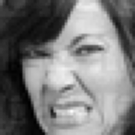
\includegraphics[interpolate=true,width=1.350000in,height=1.350000in]{fer2013-images-img0.png}}%
\end{pgfscope}%
\begin{pgfscope}%
\definecolor{textcolor}{rgb}{0.000000,0.000000,0.000000}%
\pgfsetstrokecolor{textcolor}%
\pgfsetfillcolor{textcolor}%
\pgftext[x=0.723566in,y=3.160466in,,base]{\color{textcolor}\rmfamily\fontsize{12.000000}{14.400000}\selectfont empört}%
\end{pgfscope}%
\begin{pgfscope}%
\pgfpathrectangle{\pgfqpoint{1.666559in}{1.730000in}}{\pgfqpoint{1.347132in}{1.347132in}}%
\pgfusepath{clip}%
\pgfsys@transformshift{1.666559in}{1.730000in}%
\pgftext[left,bottom]{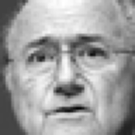
\includegraphics[interpolate=true,width=1.350000in,height=1.350000in]{fer2013-images-img1.png}}%
\end{pgfscope}%
\begin{pgfscope}%
\definecolor{textcolor}{rgb}{0.000000,0.000000,0.000000}%
\pgfsetstrokecolor{textcolor}%
\pgfsetfillcolor{textcolor}%
\pgftext[x=2.340125in,y=3.160466in,,base]{\color{textcolor}\rmfamily\fontsize{12.000000}{14.400000}\selectfont ängstlich}%
\end{pgfscope}%
\begin{pgfscope}%
\pgfpathrectangle{\pgfqpoint{3.283118in}{1.730000in}}{\pgfqpoint{1.347132in}{1.347132in}}%
\pgfusepath{clip}%
\pgfsys@transformshift{3.283118in}{1.730000in}%
\pgftext[left,bottom]{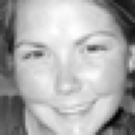
\includegraphics[interpolate=true,width=1.350000in,height=1.350000in]{fer2013-images-img2.png}}%
\end{pgfscope}%
\begin{pgfscope}%
\definecolor{textcolor}{rgb}{0.000000,0.000000,0.000000}%
\pgfsetstrokecolor{textcolor}%
\pgfsetfillcolor{textcolor}%
\pgftext[x=3.956684in,y=3.160466in,,base]{\color{textcolor}\rmfamily\fontsize{12.000000}{14.400000}\selectfont glücklich}%
\end{pgfscope}%
\begin{pgfscope}%
\pgfpathrectangle{\pgfqpoint{0.050000in}{0.050000in}}{\pgfqpoint{1.347132in}{1.347132in}}%
\pgfusepath{clip}%
\pgfsys@transformshift{0.050000in}{0.050000in}%
\pgftext[left,bottom]{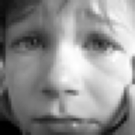
\includegraphics[interpolate=true,width=1.350000in,height=1.350000in]{fer2013-images-img3.png}}%
\end{pgfscope}%
\begin{pgfscope}%
\definecolor{textcolor}{rgb}{0.000000,0.000000,0.000000}%
\pgfsetstrokecolor{textcolor}%
\pgfsetfillcolor{textcolor}%
\pgftext[x=0.723566in,y=1.480466in,,base]{\color{textcolor}\rmfamily\fontsize{12.000000}{14.400000}\selectfont traurig}%
\end{pgfscope}%
\begin{pgfscope}%
\pgfpathrectangle{\pgfqpoint{1.666559in}{0.050000in}}{\pgfqpoint{1.347132in}{1.347132in}}%
\pgfusepath{clip}%
\pgfsys@transformshift{1.666559in}{0.050000in}%
\pgftext[left,bottom]{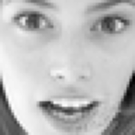
\includegraphics[interpolate=true,width=1.350000in,height=1.350000in]{fer2013-images-img4.png}}%
\end{pgfscope}%
\begin{pgfscope}%
\definecolor{textcolor}{rgb}{0.000000,0.000000,0.000000}%
\pgfsetstrokecolor{textcolor}%
\pgfsetfillcolor{textcolor}%
\pgftext[x=2.340125in,y=1.480466in,,base]{\color{textcolor}\rmfamily\fontsize{12.000000}{14.400000}\selectfont überrascht}%
\end{pgfscope}%
\begin{pgfscope}%
\pgfpathrectangle{\pgfqpoint{3.283118in}{0.050000in}}{\pgfqpoint{1.347132in}{1.347132in}}%
\pgfusepath{clip}%
\pgfsys@transformshift{3.280000in}{0.050000in}%
\pgftext[left,bottom]{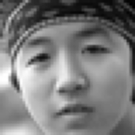
\includegraphics[interpolate=true,width=1.350000in,height=1.350000in]{fer2013-images-img5.png}}%
\end{pgfscope}%
\begin{pgfscope}%
\definecolor{textcolor}{rgb}{0.000000,0.000000,0.000000}%
\pgfsetstrokecolor{textcolor}%
\pgfsetfillcolor{textcolor}%
\pgftext[x=3.956684in,y=1.480466in,,base]{\color{textcolor}\rmfamily\fontsize{12.000000}{14.400000}\selectfont neutral}%
\end{pgfscope}%
\end{pgfpicture}%
\makeatother%
\endgroup%

	\caption[Beispielbilder des FER-Datensatzes]{Abgebildet ist je ein Bild für eine der sechs Emotionen im FER-Datensatz.}
	\label{fig:FER-Datensatz-Beispiele}
\end{figure}

\textcites{Baldi.1989}{Bourlard.1988} haben gezeigt, dass die Kodierung $\vect{y} = f(\vect{x})$ (siehe \secref{ch:MethodenDerDimRed:ML:AE:MathematischeFormulierung}) eines linearen Autoencoders äquivalent -- aber nicht identisch -- zu den Hauptkomponenten $\tr{\mat{A}}\vect{x}$ der PCA (siehe \secref{ch:MethodenDerDimRed:statistisch:PCA:HerleitungPC}) ist: Die Gewichte eines linearen Autoencoders, der den quadrierten Fehler (\eqref{eq:AE_objectiveFunction}) minimiert, spannen den gleichen Unterraum auf, wie die Ladungsmatrix $\mat{A}$. Dies gilt sogar dann, wenn im Encoder eines dreischichtigen Autoencoders Sigmoid-Aktivierungsfunktionen verwendet werden \parencite[291, 293]{Bourlard.1988}. Jedoch unterscheidet sich die latente Repräsentation $\mat{Y}$
eines linearen Autoencoders mit der von PCA wie folgt \parencite[3]{Plaut.2018}: (1) Die Kovarianzmatrix von $\mat{Y}$ ist nicht diagonal, das heißt die
latente Repräsentation ist nicht unkorreliert.\footnote{Äquivalent dazu ist die Korrelationsmatrix
	von $\mat{Y}$, welche lediglich eine skalierte Kovarianzmatrix darstellt, keine Einheitsmatrix.}
(2) Die transformierten Daten $\mat{Y}$ sind nicht nach absteigender Varianz sortiert. (3) Hat man
einen Encoder $f: \real^D \rightarrow \real^{k_1}$ und möchte man einen Vektor $\vect{x} \in
	\real^D$ auf nur $k_2$ Dimensionen mit $k_2 < k_1$ reduzieren, so können nicht einfach die ersten
$k_2$ Koordinaten von $f(\vect{x})$ verwendet werden. Das bedeutet, dass die Lösungen von
Autoencodern auf unterschiedliche Dimensionen nicht geschachtelt sind.

\begin{figure}[ht]
	\centering
	%% Creator: Matplotlib, PGF backend
%%
%% To include the figure in your LaTeX document, write
%%   \input{<filename>.pgf}
%%
%% Make sure the required packages are loaded in your preamble
%%   \usepackage{pgf}
%%
%% Also ensure that all the required font packages are loaded; for instance,
%% the lmodern package is sometimes necessary when using math font.
%%   \usepackage{lmodern}
%%
%% Figures using additional raster images can only be included by \input if
%% they are in the same directory as the main LaTeX file. For loading figures
%% from other directories you can use the `import` package
%%   \usepackage{import}
%%
%% and then include the figures with
%%   \import{<path to file>}{<filename>.pgf}
%%
%% Matplotlib used the following preamble
%%   
%%   \usepackage{fontspec}
%%   \setmainfont{DejaVuSerif.ttf}[Path=\detokenize{/Users/moritzmistol/.pyenv/versions/3.9.13/envs/thesis/lib/python3.9/site-packages/matplotlib/mpl-data/fonts/ttf/}]
%%   \setsansfont{DejaVuSans.ttf}[Path=\detokenize{/Users/moritzmistol/.pyenv/versions/3.9.13/envs/thesis/lib/python3.9/site-packages/matplotlib/mpl-data/fonts/ttf/}]
%%   \setmonofont{DejaVuSansMono.ttf}[Path=\detokenize{/Users/moritzmistol/.pyenv/versions/3.9.13/envs/thesis/lib/python3.9/site-packages/matplotlib/mpl-data/fonts/ttf/}]
%%   \makeatletter\@ifpackageloaded{underscore}{}{\usepackage[strings]{underscore}}\makeatother
%%
\begingroup%
\makeatletter%
\begin{pgfpicture}%
\pgfpathrectangle{\pgfpointorigin}{\pgfqpoint{4.390031in}{1.620413in}}%
\pgfusepath{use as bounding box, clip}%
\begin{pgfscope}%
\pgfsetbuttcap%
\pgfsetmiterjoin%
\definecolor{currentfill}{rgb}{1.000000,1.000000,1.000000}%
\pgfsetfillcolor{currentfill}%
\pgfsetlinewidth{0.000000pt}%
\definecolor{currentstroke}{rgb}{1.000000,1.000000,1.000000}%
\pgfsetstrokecolor{currentstroke}%
\pgfsetdash{}{0pt}%
\pgfpathmoveto{\pgfqpoint{0.000000in}{0.000000in}}%
\pgfpathlineto{\pgfqpoint{4.390031in}{0.000000in}}%
\pgfpathlineto{\pgfqpoint{4.390031in}{1.620413in}}%
\pgfpathlineto{\pgfqpoint{0.000000in}{1.620413in}}%
\pgfpathlineto{\pgfqpoint{0.000000in}{0.000000in}}%
\pgfpathclose%
\pgfusepath{fill}%
\end{pgfscope}%
\begin{pgfscope}%
\pgfsetbuttcap%
\pgfsetmiterjoin%
\definecolor{currentfill}{rgb}{1.000000,1.000000,1.000000}%
\pgfsetfillcolor{currentfill}%
\pgfsetlinewidth{0.000000pt}%
\definecolor{currentstroke}{rgb}{0.000000,0.000000,0.000000}%
\pgfsetstrokecolor{currentstroke}%
\pgfsetstrokeopacity{0.000000}%
\pgfsetdash{}{0pt}%
\pgfpathmoveto{\pgfqpoint{0.050000in}{0.286710in}}%
\pgfpathlineto{\pgfqpoint{1.125882in}{0.286710in}}%
\pgfpathlineto{\pgfqpoint{1.125882in}{1.362592in}}%
\pgfpathlineto{\pgfqpoint{0.050000in}{1.362592in}}%
\pgfpathlineto{\pgfqpoint{0.050000in}{0.286710in}}%
\pgfpathclose%
\pgfusepath{fill}%
\end{pgfscope}%
\begin{pgfscope}%
\pgfpathrectangle{\pgfqpoint{0.050000in}{0.286710in}}{\pgfqpoint{1.075882in}{1.075882in}}%
\pgfusepath{clip}%
\pgfsys@transformshift{0.050000in}{0.286710in}%
\pgftext[left,bottom]{
\includegraphics[interpolate=true,width=1.080000in,height=1.080000in]{correlation-matrices-img0.png}}%
\end{pgfscope}%
\begin{pgfscope}%
\pgfsetrectcap%
\pgfsetmiterjoin%
\pgfsetlinewidth{0.501875pt}%
\definecolor{currentstroke}{rgb}{0.000000,0.000000,0.000000}%
\pgfsetstrokecolor{currentstroke}%
\pgfsetdash{}{0pt}%
\pgfpathmoveto{\pgfqpoint{0.050000in}{0.286710in}}%
\pgfpathlineto{\pgfqpoint{0.050000in}{1.362592in}}%
\pgfusepath{stroke}%
\end{pgfscope}%
\begin{pgfscope}%
\pgfsetrectcap%
\pgfsetmiterjoin%
\pgfsetlinewidth{0.501875pt}%
\definecolor{currentstroke}{rgb}{0.000000,0.000000,0.000000}%
\pgfsetstrokecolor{currentstroke}%
\pgfsetdash{}{0pt}%
\pgfpathmoveto{\pgfqpoint{1.125882in}{0.286710in}}%
\pgfpathlineto{\pgfqpoint{1.125882in}{1.362592in}}%
\pgfusepath{stroke}%
\end{pgfscope}%
\begin{pgfscope}%
\pgfsetrectcap%
\pgfsetmiterjoin%
\pgfsetlinewidth{0.501875pt}%
\definecolor{currentstroke}{rgb}{0.000000,0.000000,0.000000}%
\pgfsetstrokecolor{currentstroke}%
\pgfsetdash{}{0pt}%
\pgfpathmoveto{\pgfqpoint{0.050000in}{0.286710in}}%
\pgfpathlineto{\pgfqpoint{1.125882in}{0.286710in}}%
\pgfusepath{stroke}%
\end{pgfscope}%
\begin{pgfscope}%
\pgfsetrectcap%
\pgfsetmiterjoin%
\pgfsetlinewidth{0.501875pt}%
\definecolor{currentstroke}{rgb}{0.000000,0.000000,0.000000}%
\pgfsetstrokecolor{currentstroke}%
\pgfsetdash{}{0pt}%
\pgfpathmoveto{\pgfqpoint{0.050000in}{1.362592in}}%
\pgfpathlineto{\pgfqpoint{1.125882in}{1.362592in}}%
\pgfusepath{stroke}%
\end{pgfscope}%
\begin{pgfscope}%
\pgfsetbuttcap%
\pgfsetmiterjoin%
\definecolor{currentfill}{rgb}{1.000000,1.000000,1.000000}%
\pgfsetfillcolor{currentfill}%
\pgfsetlinewidth{0.000000pt}%
\definecolor{currentstroke}{rgb}{0.000000,0.000000,0.000000}%
\pgfsetstrokecolor{currentstroke}%
\pgfsetstrokeopacity{0.000000}%
\pgfsetdash{}{0pt}%
\pgfpathmoveto{\pgfqpoint{1.341059in}{0.286710in}}%
\pgfpathlineto{\pgfqpoint{2.416941in}{0.286710in}}%
\pgfpathlineto{\pgfqpoint{2.416941in}{1.362592in}}%
\pgfpathlineto{\pgfqpoint{1.341059in}{1.362592in}}%
\pgfpathlineto{\pgfqpoint{1.341059in}{0.286710in}}%
\pgfpathclose%
\pgfusepath{fill}%
\end{pgfscope}%
\begin{pgfscope}%
\pgfpathrectangle{\pgfqpoint{1.341059in}{0.286710in}}{\pgfqpoint{1.075882in}{1.075882in}}%
\pgfusepath{clip}%
\pgfsys@transformshift{1.341059in}{0.286710in}%
\pgftext[left,bottom]{
\includegraphics[interpolate=true,width=1.080000in,height=1.080000in]{correlation-matrices-img1.png}}%
\end{pgfscope}%
\begin{pgfscope}%
\pgfsetrectcap%
\pgfsetmiterjoin%
\pgfsetlinewidth{0.501875pt}%
\definecolor{currentstroke}{rgb}{0.000000,0.000000,0.000000}%
\pgfsetstrokecolor{currentstroke}%
\pgfsetdash{}{0pt}%
\pgfpathmoveto{\pgfqpoint{1.341059in}{0.286710in}}%
\pgfpathlineto{\pgfqpoint{1.341059in}{1.362592in}}%
\pgfusepath{stroke}%
\end{pgfscope}%
\begin{pgfscope}%
\pgfsetrectcap%
\pgfsetmiterjoin%
\pgfsetlinewidth{0.501875pt}%
\definecolor{currentstroke}{rgb}{0.000000,0.000000,0.000000}%
\pgfsetstrokecolor{currentstroke}%
\pgfsetdash{}{0pt}%
\pgfpathmoveto{\pgfqpoint{2.416941in}{0.286710in}}%
\pgfpathlineto{\pgfqpoint{2.416941in}{1.362592in}}%
\pgfusepath{stroke}%
\end{pgfscope}%
\begin{pgfscope}%
\pgfsetrectcap%
\pgfsetmiterjoin%
\pgfsetlinewidth{0.501875pt}%
\definecolor{currentstroke}{rgb}{0.000000,0.000000,0.000000}%
\pgfsetstrokecolor{currentstroke}%
\pgfsetdash{}{0pt}%
\pgfpathmoveto{\pgfqpoint{1.341059in}{0.286710in}}%
\pgfpathlineto{\pgfqpoint{2.416941in}{0.286710in}}%
\pgfusepath{stroke}%
\end{pgfscope}%
\begin{pgfscope}%
\pgfsetrectcap%
\pgfsetmiterjoin%
\pgfsetlinewidth{0.501875pt}%
\definecolor{currentstroke}{rgb}{0.000000,0.000000,0.000000}%
\pgfsetstrokecolor{currentstroke}%
\pgfsetdash{}{0pt}%
\pgfpathmoveto{\pgfqpoint{1.341059in}{1.362592in}}%
\pgfpathlineto{\pgfqpoint{2.416941in}{1.362592in}}%
\pgfusepath{stroke}%
\end{pgfscope}%
\begin{pgfscope}%
\pgfsetbuttcap%
\pgfsetmiterjoin%
\definecolor{currentfill}{rgb}{1.000000,1.000000,1.000000}%
\pgfsetfillcolor{currentfill}%
\pgfsetlinewidth{0.000000pt}%
\definecolor{currentstroke}{rgb}{0.000000,0.000000,0.000000}%
\pgfsetstrokecolor{currentstroke}%
\pgfsetstrokeopacity{0.000000}%
\pgfsetdash{}{0pt}%
\pgfpathmoveto{\pgfqpoint{2.632118in}{0.286710in}}%
\pgfpathlineto{\pgfqpoint{3.708000in}{0.286710in}}%
\pgfpathlineto{\pgfqpoint{3.708000in}{1.362592in}}%
\pgfpathlineto{\pgfqpoint{2.632118in}{1.362592in}}%
\pgfpathlineto{\pgfqpoint{2.632118in}{0.286710in}}%
\pgfpathclose%
\pgfusepath{fill}%
\end{pgfscope}%
\begin{pgfscope}%
\pgfpathrectangle{\pgfqpoint{2.632118in}{0.286710in}}{\pgfqpoint{1.075882in}{1.075882in}}%
\pgfusepath{clip}%
\pgfsys@transformshift{2.632118in}{0.286710in}%
\pgftext[left,bottom]{
\includegraphics[interpolate=true,width=1.080000in,height=1.080000in]{correlation-matrices-img2.png}}%
\end{pgfscope}%
\begin{pgfscope}%
\pgfsetrectcap%
\pgfsetmiterjoin%
\pgfsetlinewidth{0.501875pt}%
\definecolor{currentstroke}{rgb}{0.000000,0.000000,0.000000}%
\pgfsetstrokecolor{currentstroke}%
\pgfsetdash{}{0pt}%
\pgfpathmoveto{\pgfqpoint{2.632118in}{0.286710in}}%
\pgfpathlineto{\pgfqpoint{2.632118in}{1.362592in}}%
\pgfusepath{stroke}%
\end{pgfscope}%
\begin{pgfscope}%
\pgfsetrectcap%
\pgfsetmiterjoin%
\pgfsetlinewidth{0.501875pt}%
\definecolor{currentstroke}{rgb}{0.000000,0.000000,0.000000}%
\pgfsetstrokecolor{currentstroke}%
\pgfsetdash{}{0pt}%
\pgfpathmoveto{\pgfqpoint{3.708000in}{0.286710in}}%
\pgfpathlineto{\pgfqpoint{3.708000in}{1.362592in}}%
\pgfusepath{stroke}%
\end{pgfscope}%
\begin{pgfscope}%
\pgfsetrectcap%
\pgfsetmiterjoin%
\pgfsetlinewidth{0.501875pt}%
\definecolor{currentstroke}{rgb}{0.000000,0.000000,0.000000}%
\pgfsetstrokecolor{currentstroke}%
\pgfsetdash{}{0pt}%
\pgfpathmoveto{\pgfqpoint{2.632118in}{0.286710in}}%
\pgfpathlineto{\pgfqpoint{3.708000in}{0.286710in}}%
\pgfusepath{stroke}%
\end{pgfscope}%
\begin{pgfscope}%
\pgfsetrectcap%
\pgfsetmiterjoin%
\pgfsetlinewidth{0.501875pt}%
\definecolor{currentstroke}{rgb}{0.000000,0.000000,0.000000}%
\pgfsetstrokecolor{currentstroke}%
\pgfsetdash{}{0pt}%
\pgfpathmoveto{\pgfqpoint{2.632118in}{1.362592in}}%
\pgfpathlineto{\pgfqpoint{3.708000in}{1.362592in}}%
\pgfusepath{stroke}%
\end{pgfscope}%
\begin{pgfscope}%
\definecolor{textcolor}{rgb}{0.000000,0.000000,0.000000}%
\pgfsetstrokecolor{textcolor}%
\pgfsetfillcolor{textcolor}%
\pgftext[x=0.587941in,y=0.179122in,,]{\color{textcolor}\rmfamily\fontsize{10.000000}{12.000000}\selectfont (a)}%
\end{pgfscope}%
\begin{pgfscope}%
\definecolor{textcolor}{rgb}{0.000000,0.000000,0.000000}%
\pgfsetstrokecolor{textcolor}%
\pgfsetfillcolor{textcolor}%
\pgftext[x=1.879000in,y=0.179122in,,]{\color{textcolor}\rmfamily\fontsize{10.000000}{12.000000}\selectfont (b)}%
\end{pgfscope}%
\begin{pgfscope}%
\definecolor{textcolor}{rgb}{0.000000,0.000000,0.000000}%
\pgfsetstrokecolor{textcolor}%
\pgfsetfillcolor{textcolor}%
\pgftext[x=3.170059in,y=0.179122in,,]{\color{textcolor}\rmfamily\fontsize{10.000000}{12.000000}\selectfont (c)}%
\end{pgfscope}%
\begin{pgfscope}%
\pgfsetbuttcap%
\pgfsetmiterjoin%
\definecolor{currentfill}{rgb}{1.000000,1.000000,1.000000}%
\pgfsetfillcolor{currentfill}%
\pgfsetlinewidth{0.000000pt}%
\definecolor{currentstroke}{rgb}{0.000000,0.000000,0.000000}%
\pgfsetstrokecolor{currentstroke}%
\pgfsetstrokeopacity{0.000000}%
\pgfsetdash{}{0pt}%
\pgfpathmoveto{\pgfqpoint{3.936625in}{0.131651in}}%
\pgfpathlineto{\pgfqpoint{4.005925in}{0.131651in}}%
\pgfpathlineto{\pgfqpoint{4.005925in}{1.517651in}}%
\pgfpathlineto{\pgfqpoint{3.936625in}{1.517651in}}%
\pgfpathlineto{\pgfqpoint{3.936625in}{0.131651in}}%
\pgfpathclose%
\pgfusepath{fill}%
\end{pgfscope}%
\begin{pgfscope}%
\pgfpathrectangle{\pgfqpoint{3.936625in}{0.131651in}}{\pgfqpoint{0.069300in}{1.386000in}}%
\pgfusepath{clip}%
\pgfsetbuttcap%
\pgfsetmiterjoin%
\definecolor{currentfill}{rgb}{1.000000,1.000000,1.000000}%
\pgfsetfillcolor{currentfill}%
\pgfsetlinewidth{0.010037pt}%
\definecolor{currentstroke}{rgb}{1.000000,1.000000,1.000000}%
\pgfsetstrokecolor{currentstroke}%
\pgfsetdash{}{0pt}%
\pgfusepath{stroke,fill}%
\end{pgfscope}%
\begin{pgfscope}%
\pgfsys@transformshift{3.940000in}{0.130413in}%
\pgftext[left,bottom]{
\includegraphics[interpolate=true,width=0.070000in,height=1.390000in]{correlation-matrices-img3.png}}%
\end{pgfscope}%
\begin{pgfscope}%
\pgfsetbuttcap%
\pgfsetroundjoin%
\definecolor{currentfill}{rgb}{0.000000,0.000000,0.000000}%
\pgfsetfillcolor{currentfill}%
\pgfsetlinewidth{0.501875pt}%
\definecolor{currentstroke}{rgb}{0.000000,0.000000,0.000000}%
\pgfsetstrokecolor{currentstroke}%
\pgfsetdash{}{0pt}%
\pgfsys@defobject{currentmarker}{\pgfqpoint{-0.041667in}{0.000000in}}{\pgfqpoint{-0.000000in}{0.000000in}}{%
\pgfpathmoveto{\pgfqpoint{-0.000000in}{0.000000in}}%
\pgfpathlineto{\pgfqpoint{-0.041667in}{0.000000in}}%
\pgfusepath{stroke,fill}%
}%
\begin{pgfscope}%
\pgfsys@transformshift{4.005925in}{0.131651in}%
\pgfsys@useobject{currentmarker}{}%
\end{pgfscope}%
\end{pgfscope}%
\begin{pgfscope}%
\definecolor{textcolor}{rgb}{0.000000,0.000000,0.000000}%
\pgfsetstrokecolor{textcolor}%
\pgfsetfillcolor{textcolor}%
\pgftext[x=4.054536in, y=0.078890in, left, base]{\color{textcolor}\rmfamily\fontsize{10.000000}{12.000000}\selectfont \(\displaystyle {\ensuremath{-}1.0}\)}%
\end{pgfscope}%
\begin{pgfscope}%
\pgfsetbuttcap%
\pgfsetroundjoin%
\definecolor{currentfill}{rgb}{0.000000,0.000000,0.000000}%
\pgfsetfillcolor{currentfill}%
\pgfsetlinewidth{0.501875pt}%
\definecolor{currentstroke}{rgb}{0.000000,0.000000,0.000000}%
\pgfsetstrokecolor{currentstroke}%
\pgfsetdash{}{0pt}%
\pgfsys@defobject{currentmarker}{\pgfqpoint{-0.041667in}{0.000000in}}{\pgfqpoint{-0.000000in}{0.000000in}}{%
\pgfpathmoveto{\pgfqpoint{-0.000000in}{0.000000in}}%
\pgfpathlineto{\pgfqpoint{-0.041667in}{0.000000in}}%
\pgfusepath{stroke,fill}%
}%
\begin{pgfscope}%
\pgfsys@transformshift{4.005925in}{0.478151in}%
\pgfsys@useobject{currentmarker}{}%
\end{pgfscope}%
\end{pgfscope}%
\begin{pgfscope}%
\definecolor{textcolor}{rgb}{0.000000,0.000000,0.000000}%
\pgfsetstrokecolor{textcolor}%
\pgfsetfillcolor{textcolor}%
\pgftext[x=4.054536in, y=0.425390in, left, base]{\color{textcolor}\rmfamily\fontsize{10.000000}{12.000000}\selectfont \(\displaystyle {\ensuremath{-}0.5}\)}%
\end{pgfscope}%
\begin{pgfscope}%
\pgfsetbuttcap%
\pgfsetroundjoin%
\definecolor{currentfill}{rgb}{0.000000,0.000000,0.000000}%
\pgfsetfillcolor{currentfill}%
\pgfsetlinewidth{0.501875pt}%
\definecolor{currentstroke}{rgb}{0.000000,0.000000,0.000000}%
\pgfsetstrokecolor{currentstroke}%
\pgfsetdash{}{0pt}%
\pgfsys@defobject{currentmarker}{\pgfqpoint{-0.041667in}{0.000000in}}{\pgfqpoint{-0.000000in}{0.000000in}}{%
\pgfpathmoveto{\pgfqpoint{-0.000000in}{0.000000in}}%
\pgfpathlineto{\pgfqpoint{-0.041667in}{0.000000in}}%
\pgfusepath{stroke,fill}%
}%
\begin{pgfscope}%
\pgfsys@transformshift{4.005925in}{0.824651in}%
\pgfsys@useobject{currentmarker}{}%
\end{pgfscope}%
\end{pgfscope}%
\begin{pgfscope}%
\definecolor{textcolor}{rgb}{0.000000,0.000000,0.000000}%
\pgfsetstrokecolor{textcolor}%
\pgfsetfillcolor{textcolor}%
\pgftext[x=4.054536in, y=0.771890in, left, base]{\color{textcolor}\rmfamily\fontsize{10.000000}{12.000000}\selectfont \(\displaystyle {0.0}\)}%
\end{pgfscope}%
\begin{pgfscope}%
\pgfsetbuttcap%
\pgfsetroundjoin%
\definecolor{currentfill}{rgb}{0.000000,0.000000,0.000000}%
\pgfsetfillcolor{currentfill}%
\pgfsetlinewidth{0.501875pt}%
\definecolor{currentstroke}{rgb}{0.000000,0.000000,0.000000}%
\pgfsetstrokecolor{currentstroke}%
\pgfsetdash{}{0pt}%
\pgfsys@defobject{currentmarker}{\pgfqpoint{-0.041667in}{0.000000in}}{\pgfqpoint{-0.000000in}{0.000000in}}{%
\pgfpathmoveto{\pgfqpoint{-0.000000in}{0.000000in}}%
\pgfpathlineto{\pgfqpoint{-0.041667in}{0.000000in}}%
\pgfusepath{stroke,fill}%
}%
\begin{pgfscope}%
\pgfsys@transformshift{4.005925in}{1.171151in}%
\pgfsys@useobject{currentmarker}{}%
\end{pgfscope}%
\end{pgfscope}%
\begin{pgfscope}%
\definecolor{textcolor}{rgb}{0.000000,0.000000,0.000000}%
\pgfsetstrokecolor{textcolor}%
\pgfsetfillcolor{textcolor}%
\pgftext[x=4.054536in, y=1.118390in, left, base]{\color{textcolor}\rmfamily\fontsize{10.000000}{12.000000}\selectfont \(\displaystyle {0.5}\)}%
\end{pgfscope}%
\begin{pgfscope}%
\pgfsetbuttcap%
\pgfsetroundjoin%
\definecolor{currentfill}{rgb}{0.000000,0.000000,0.000000}%
\pgfsetfillcolor{currentfill}%
\pgfsetlinewidth{0.501875pt}%
\definecolor{currentstroke}{rgb}{0.000000,0.000000,0.000000}%
\pgfsetstrokecolor{currentstroke}%
\pgfsetdash{}{0pt}%
\pgfsys@defobject{currentmarker}{\pgfqpoint{-0.041667in}{0.000000in}}{\pgfqpoint{-0.000000in}{0.000000in}}{%
\pgfpathmoveto{\pgfqpoint{-0.000000in}{0.000000in}}%
\pgfpathlineto{\pgfqpoint{-0.041667in}{0.000000in}}%
\pgfusepath{stroke,fill}%
}%
\begin{pgfscope}%
\pgfsys@transformshift{4.005925in}{1.517651in}%
\pgfsys@useobject{currentmarker}{}%
\end{pgfscope}%
\end{pgfscope}%
\begin{pgfscope}%
\definecolor{textcolor}{rgb}{0.000000,0.000000,0.000000}%
\pgfsetstrokecolor{textcolor}%
\pgfsetfillcolor{textcolor}%
\pgftext[x=4.054536in, y=1.464890in, left, base]{\color{textcolor}\rmfamily\fontsize{10.000000}{12.000000}\selectfont \(\displaystyle {1.0}\)}%
\end{pgfscope}%
\begin{pgfscope}%
\pgfsetbuttcap%
\pgfsetroundjoin%
\definecolor{currentfill}{rgb}{0.000000,0.000000,0.000000}%
\pgfsetfillcolor{currentfill}%
\pgfsetlinewidth{0.501875pt}%
\definecolor{currentstroke}{rgb}{0.000000,0.000000,0.000000}%
\pgfsetstrokecolor{currentstroke}%
\pgfsetdash{}{0pt}%
\pgfsys@defobject{currentmarker}{\pgfqpoint{-0.020833in}{0.000000in}}{\pgfqpoint{-0.000000in}{0.000000in}}{%
\pgfpathmoveto{\pgfqpoint{-0.000000in}{0.000000in}}%
\pgfpathlineto{\pgfqpoint{-0.020833in}{0.000000in}}%
\pgfusepath{stroke,fill}%
}%
\begin{pgfscope}%
\pgfsys@transformshift{4.005925in}{0.200951in}%
\pgfsys@useobject{currentmarker}{}%
\end{pgfscope}%
\end{pgfscope}%
\begin{pgfscope}%
\pgfsetbuttcap%
\pgfsetroundjoin%
\definecolor{currentfill}{rgb}{0.000000,0.000000,0.000000}%
\pgfsetfillcolor{currentfill}%
\pgfsetlinewidth{0.501875pt}%
\definecolor{currentstroke}{rgb}{0.000000,0.000000,0.000000}%
\pgfsetstrokecolor{currentstroke}%
\pgfsetdash{}{0pt}%
\pgfsys@defobject{currentmarker}{\pgfqpoint{-0.020833in}{0.000000in}}{\pgfqpoint{-0.000000in}{0.000000in}}{%
\pgfpathmoveto{\pgfqpoint{-0.000000in}{0.000000in}}%
\pgfpathlineto{\pgfqpoint{-0.020833in}{0.000000in}}%
\pgfusepath{stroke,fill}%
}%
\begin{pgfscope}%
\pgfsys@transformshift{4.005925in}{0.270251in}%
\pgfsys@useobject{currentmarker}{}%
\end{pgfscope}%
\end{pgfscope}%
\begin{pgfscope}%
\pgfsetbuttcap%
\pgfsetroundjoin%
\definecolor{currentfill}{rgb}{0.000000,0.000000,0.000000}%
\pgfsetfillcolor{currentfill}%
\pgfsetlinewidth{0.501875pt}%
\definecolor{currentstroke}{rgb}{0.000000,0.000000,0.000000}%
\pgfsetstrokecolor{currentstroke}%
\pgfsetdash{}{0pt}%
\pgfsys@defobject{currentmarker}{\pgfqpoint{-0.020833in}{0.000000in}}{\pgfqpoint{-0.000000in}{0.000000in}}{%
\pgfpathmoveto{\pgfqpoint{-0.000000in}{0.000000in}}%
\pgfpathlineto{\pgfqpoint{-0.020833in}{0.000000in}}%
\pgfusepath{stroke,fill}%
}%
\begin{pgfscope}%
\pgfsys@transformshift{4.005925in}{0.339551in}%
\pgfsys@useobject{currentmarker}{}%
\end{pgfscope}%
\end{pgfscope}%
\begin{pgfscope}%
\pgfsetbuttcap%
\pgfsetroundjoin%
\definecolor{currentfill}{rgb}{0.000000,0.000000,0.000000}%
\pgfsetfillcolor{currentfill}%
\pgfsetlinewidth{0.501875pt}%
\definecolor{currentstroke}{rgb}{0.000000,0.000000,0.000000}%
\pgfsetstrokecolor{currentstroke}%
\pgfsetdash{}{0pt}%
\pgfsys@defobject{currentmarker}{\pgfqpoint{-0.020833in}{0.000000in}}{\pgfqpoint{-0.000000in}{0.000000in}}{%
\pgfpathmoveto{\pgfqpoint{-0.000000in}{0.000000in}}%
\pgfpathlineto{\pgfqpoint{-0.020833in}{0.000000in}}%
\pgfusepath{stroke,fill}%
}%
\begin{pgfscope}%
\pgfsys@transformshift{4.005925in}{0.408851in}%
\pgfsys@useobject{currentmarker}{}%
\end{pgfscope}%
\end{pgfscope}%
\begin{pgfscope}%
\pgfsetbuttcap%
\pgfsetroundjoin%
\definecolor{currentfill}{rgb}{0.000000,0.000000,0.000000}%
\pgfsetfillcolor{currentfill}%
\pgfsetlinewidth{0.501875pt}%
\definecolor{currentstroke}{rgb}{0.000000,0.000000,0.000000}%
\pgfsetstrokecolor{currentstroke}%
\pgfsetdash{}{0pt}%
\pgfsys@defobject{currentmarker}{\pgfqpoint{-0.020833in}{0.000000in}}{\pgfqpoint{-0.000000in}{0.000000in}}{%
\pgfpathmoveto{\pgfqpoint{-0.000000in}{0.000000in}}%
\pgfpathlineto{\pgfqpoint{-0.020833in}{0.000000in}}%
\pgfusepath{stroke,fill}%
}%
\begin{pgfscope}%
\pgfsys@transformshift{4.005925in}{0.547451in}%
\pgfsys@useobject{currentmarker}{}%
\end{pgfscope}%
\end{pgfscope}%
\begin{pgfscope}%
\pgfsetbuttcap%
\pgfsetroundjoin%
\definecolor{currentfill}{rgb}{0.000000,0.000000,0.000000}%
\pgfsetfillcolor{currentfill}%
\pgfsetlinewidth{0.501875pt}%
\definecolor{currentstroke}{rgb}{0.000000,0.000000,0.000000}%
\pgfsetstrokecolor{currentstroke}%
\pgfsetdash{}{0pt}%
\pgfsys@defobject{currentmarker}{\pgfqpoint{-0.020833in}{0.000000in}}{\pgfqpoint{-0.000000in}{0.000000in}}{%
\pgfpathmoveto{\pgfqpoint{-0.000000in}{0.000000in}}%
\pgfpathlineto{\pgfqpoint{-0.020833in}{0.000000in}}%
\pgfusepath{stroke,fill}%
}%
\begin{pgfscope}%
\pgfsys@transformshift{4.005925in}{0.616751in}%
\pgfsys@useobject{currentmarker}{}%
\end{pgfscope}%
\end{pgfscope}%
\begin{pgfscope}%
\pgfsetbuttcap%
\pgfsetroundjoin%
\definecolor{currentfill}{rgb}{0.000000,0.000000,0.000000}%
\pgfsetfillcolor{currentfill}%
\pgfsetlinewidth{0.501875pt}%
\definecolor{currentstroke}{rgb}{0.000000,0.000000,0.000000}%
\pgfsetstrokecolor{currentstroke}%
\pgfsetdash{}{0pt}%
\pgfsys@defobject{currentmarker}{\pgfqpoint{-0.020833in}{0.000000in}}{\pgfqpoint{-0.000000in}{0.000000in}}{%
\pgfpathmoveto{\pgfqpoint{-0.000000in}{0.000000in}}%
\pgfpathlineto{\pgfqpoint{-0.020833in}{0.000000in}}%
\pgfusepath{stroke,fill}%
}%
\begin{pgfscope}%
\pgfsys@transformshift{4.005925in}{0.686051in}%
\pgfsys@useobject{currentmarker}{}%
\end{pgfscope}%
\end{pgfscope}%
\begin{pgfscope}%
\pgfsetbuttcap%
\pgfsetroundjoin%
\definecolor{currentfill}{rgb}{0.000000,0.000000,0.000000}%
\pgfsetfillcolor{currentfill}%
\pgfsetlinewidth{0.501875pt}%
\definecolor{currentstroke}{rgb}{0.000000,0.000000,0.000000}%
\pgfsetstrokecolor{currentstroke}%
\pgfsetdash{}{0pt}%
\pgfsys@defobject{currentmarker}{\pgfqpoint{-0.020833in}{0.000000in}}{\pgfqpoint{-0.000000in}{0.000000in}}{%
\pgfpathmoveto{\pgfqpoint{-0.000000in}{0.000000in}}%
\pgfpathlineto{\pgfqpoint{-0.020833in}{0.000000in}}%
\pgfusepath{stroke,fill}%
}%
\begin{pgfscope}%
\pgfsys@transformshift{4.005925in}{0.755351in}%
\pgfsys@useobject{currentmarker}{}%
\end{pgfscope}%
\end{pgfscope}%
\begin{pgfscope}%
\pgfsetbuttcap%
\pgfsetroundjoin%
\definecolor{currentfill}{rgb}{0.000000,0.000000,0.000000}%
\pgfsetfillcolor{currentfill}%
\pgfsetlinewidth{0.501875pt}%
\definecolor{currentstroke}{rgb}{0.000000,0.000000,0.000000}%
\pgfsetstrokecolor{currentstroke}%
\pgfsetdash{}{0pt}%
\pgfsys@defobject{currentmarker}{\pgfqpoint{-0.020833in}{0.000000in}}{\pgfqpoint{-0.000000in}{0.000000in}}{%
\pgfpathmoveto{\pgfqpoint{-0.000000in}{0.000000in}}%
\pgfpathlineto{\pgfqpoint{-0.020833in}{0.000000in}}%
\pgfusepath{stroke,fill}%
}%
\begin{pgfscope}%
\pgfsys@transformshift{4.005925in}{0.893951in}%
\pgfsys@useobject{currentmarker}{}%
\end{pgfscope}%
\end{pgfscope}%
\begin{pgfscope}%
\pgfsetbuttcap%
\pgfsetroundjoin%
\definecolor{currentfill}{rgb}{0.000000,0.000000,0.000000}%
\pgfsetfillcolor{currentfill}%
\pgfsetlinewidth{0.501875pt}%
\definecolor{currentstroke}{rgb}{0.000000,0.000000,0.000000}%
\pgfsetstrokecolor{currentstroke}%
\pgfsetdash{}{0pt}%
\pgfsys@defobject{currentmarker}{\pgfqpoint{-0.020833in}{0.000000in}}{\pgfqpoint{-0.000000in}{0.000000in}}{%
\pgfpathmoveto{\pgfqpoint{-0.000000in}{0.000000in}}%
\pgfpathlineto{\pgfqpoint{-0.020833in}{0.000000in}}%
\pgfusepath{stroke,fill}%
}%
\begin{pgfscope}%
\pgfsys@transformshift{4.005925in}{0.963251in}%
\pgfsys@useobject{currentmarker}{}%
\end{pgfscope}%
\end{pgfscope}%
\begin{pgfscope}%
\pgfsetbuttcap%
\pgfsetroundjoin%
\definecolor{currentfill}{rgb}{0.000000,0.000000,0.000000}%
\pgfsetfillcolor{currentfill}%
\pgfsetlinewidth{0.501875pt}%
\definecolor{currentstroke}{rgb}{0.000000,0.000000,0.000000}%
\pgfsetstrokecolor{currentstroke}%
\pgfsetdash{}{0pt}%
\pgfsys@defobject{currentmarker}{\pgfqpoint{-0.020833in}{0.000000in}}{\pgfqpoint{-0.000000in}{0.000000in}}{%
\pgfpathmoveto{\pgfqpoint{-0.000000in}{0.000000in}}%
\pgfpathlineto{\pgfqpoint{-0.020833in}{0.000000in}}%
\pgfusepath{stroke,fill}%
}%
\begin{pgfscope}%
\pgfsys@transformshift{4.005925in}{1.032551in}%
\pgfsys@useobject{currentmarker}{}%
\end{pgfscope}%
\end{pgfscope}%
\begin{pgfscope}%
\pgfsetbuttcap%
\pgfsetroundjoin%
\definecolor{currentfill}{rgb}{0.000000,0.000000,0.000000}%
\pgfsetfillcolor{currentfill}%
\pgfsetlinewidth{0.501875pt}%
\definecolor{currentstroke}{rgb}{0.000000,0.000000,0.000000}%
\pgfsetstrokecolor{currentstroke}%
\pgfsetdash{}{0pt}%
\pgfsys@defobject{currentmarker}{\pgfqpoint{-0.020833in}{0.000000in}}{\pgfqpoint{-0.000000in}{0.000000in}}{%
\pgfpathmoveto{\pgfqpoint{-0.000000in}{0.000000in}}%
\pgfpathlineto{\pgfqpoint{-0.020833in}{0.000000in}}%
\pgfusepath{stroke,fill}%
}%
\begin{pgfscope}%
\pgfsys@transformshift{4.005925in}{1.101851in}%
\pgfsys@useobject{currentmarker}{}%
\end{pgfscope}%
\end{pgfscope}%
\begin{pgfscope}%
\pgfsetbuttcap%
\pgfsetroundjoin%
\definecolor{currentfill}{rgb}{0.000000,0.000000,0.000000}%
\pgfsetfillcolor{currentfill}%
\pgfsetlinewidth{0.501875pt}%
\definecolor{currentstroke}{rgb}{0.000000,0.000000,0.000000}%
\pgfsetstrokecolor{currentstroke}%
\pgfsetdash{}{0pt}%
\pgfsys@defobject{currentmarker}{\pgfqpoint{-0.020833in}{0.000000in}}{\pgfqpoint{-0.000000in}{0.000000in}}{%
\pgfpathmoveto{\pgfqpoint{-0.000000in}{0.000000in}}%
\pgfpathlineto{\pgfqpoint{-0.020833in}{0.000000in}}%
\pgfusepath{stroke,fill}%
}%
\begin{pgfscope}%
\pgfsys@transformshift{4.005925in}{1.240451in}%
\pgfsys@useobject{currentmarker}{}%
\end{pgfscope}%
\end{pgfscope}%
\begin{pgfscope}%
\pgfsetbuttcap%
\pgfsetroundjoin%
\definecolor{currentfill}{rgb}{0.000000,0.000000,0.000000}%
\pgfsetfillcolor{currentfill}%
\pgfsetlinewidth{0.501875pt}%
\definecolor{currentstroke}{rgb}{0.000000,0.000000,0.000000}%
\pgfsetstrokecolor{currentstroke}%
\pgfsetdash{}{0pt}%
\pgfsys@defobject{currentmarker}{\pgfqpoint{-0.020833in}{0.000000in}}{\pgfqpoint{-0.000000in}{0.000000in}}{%
\pgfpathmoveto{\pgfqpoint{-0.000000in}{0.000000in}}%
\pgfpathlineto{\pgfqpoint{-0.020833in}{0.000000in}}%
\pgfusepath{stroke,fill}%
}%
\begin{pgfscope}%
\pgfsys@transformshift{4.005925in}{1.309751in}%
\pgfsys@useobject{currentmarker}{}%
\end{pgfscope}%
\end{pgfscope}%
\begin{pgfscope}%
\pgfsetbuttcap%
\pgfsetroundjoin%
\definecolor{currentfill}{rgb}{0.000000,0.000000,0.000000}%
\pgfsetfillcolor{currentfill}%
\pgfsetlinewidth{0.501875pt}%
\definecolor{currentstroke}{rgb}{0.000000,0.000000,0.000000}%
\pgfsetstrokecolor{currentstroke}%
\pgfsetdash{}{0pt}%
\pgfsys@defobject{currentmarker}{\pgfqpoint{-0.020833in}{0.000000in}}{\pgfqpoint{-0.000000in}{0.000000in}}{%
\pgfpathmoveto{\pgfqpoint{-0.000000in}{0.000000in}}%
\pgfpathlineto{\pgfqpoint{-0.020833in}{0.000000in}}%
\pgfusepath{stroke,fill}%
}%
\begin{pgfscope}%
\pgfsys@transformshift{4.005925in}{1.379051in}%
\pgfsys@useobject{currentmarker}{}%
\end{pgfscope}%
\end{pgfscope}%
\begin{pgfscope}%
\pgfsetbuttcap%
\pgfsetroundjoin%
\definecolor{currentfill}{rgb}{0.000000,0.000000,0.000000}%
\pgfsetfillcolor{currentfill}%
\pgfsetlinewidth{0.501875pt}%
\definecolor{currentstroke}{rgb}{0.000000,0.000000,0.000000}%
\pgfsetstrokecolor{currentstroke}%
\pgfsetdash{}{0pt}%
\pgfsys@defobject{currentmarker}{\pgfqpoint{-0.020833in}{0.000000in}}{\pgfqpoint{-0.000000in}{0.000000in}}{%
\pgfpathmoveto{\pgfqpoint{-0.000000in}{0.000000in}}%
\pgfpathlineto{\pgfqpoint{-0.020833in}{0.000000in}}%
\pgfusepath{stroke,fill}%
}%
\begin{pgfscope}%
\pgfsys@transformshift{4.005925in}{1.448351in}%
\pgfsys@useobject{currentmarker}{}%
\end{pgfscope}%
\end{pgfscope}%
\begin{pgfscope}%
\pgfsetrectcap%
\pgfsetmiterjoin%
\pgfsetlinewidth{0.501875pt}%
\definecolor{currentstroke}{rgb}{0.000000,0.000000,0.000000}%
\pgfsetstrokecolor{currentstroke}%
\pgfsetdash{}{0pt}%
\pgfpathmoveto{\pgfqpoint{3.936625in}{0.131651in}}%
\pgfpathlineto{\pgfqpoint{3.971275in}{0.131651in}}%
\pgfpathlineto{\pgfqpoint{4.005925in}{0.131651in}}%
\pgfpathlineto{\pgfqpoint{4.005925in}{1.517651in}}%
\pgfpathlineto{\pgfqpoint{3.971275in}{1.517651in}}%
\pgfpathlineto{\pgfqpoint{3.936625in}{1.517651in}}%
\pgfpathlineto{\pgfqpoint{3.936625in}{0.131651in}}%
\pgfpathclose%
\pgfusepath{stroke}%
\end{pgfscope}%
\end{pgfpicture}%
\makeatother%
\endgroup%

	\caption[Korrelationsmatrizen der transformierten Daten $\mat{Y}$ für den FER-Datensatz von vier Methoden]{Hier sind die Korrelationsmatrizen der transformierten Daten $\mat{Y}$ für den FER-Datensatz abgebildet, wobei in \captiona die Hauptkomponentenanalyse, in \captionb ein linearer dreischichtiger Autoencoder und in \captionc ein nichtlinearer dreischichtiger Autoencoder mit Sigmoid-Encoder und linearem Decoder verwendet wurde, um die Daten auf sechs Dimensionen zu reduzieren. Die Korrelationsmatrix bei Transformation mittels der Hauptkomponentenanalyse ist per Konstruktion eine Einheitsmatrix, das heißt es besteht keine Korrelation in $\mat{Y}$. Bei Transformation durch die Autoencoder besteht Korrelation, wobei der lineare Autoencoder zufälligerweise betragsmäßig größere Korrelationen erzeugt als der nichtlineare Autoencoder.  (Eigene Darstellung, angelehnt an \textcite[5]{Plaut.2018})}
	\label{fig:Korrelationsmatrizen}
\end{figure}
Punkt 1 ist in beispielsweise in \figref{fig:Korrelationsmatrizen} zu erkennen. Dargestellt sind die Korrelationsmatrizen der transformierten Daten, wobei in \captiona die Hauptkomponentenanalyse, in \captionb ein linearer dreischichtiger Autoencoder und in \captionc und (d) nichtlineare Autoencoder verwendet wurden. Die Korrelationsmatrix der Hauptkomponentenanalyse ist eine Einheitsmatrix, während die Korrelationsmatrizen der durch die Autoencoder gefundenen latenten Repräsentationen von Null verschiedene Werte auf der Nicht-diagonalen aufweisen.

Um die gefundenen Lösungen einer Hauptkomponentenanalyse und von Autoencodern genauer betrachten zu
können, kann die Ladungsmatrix $\mat{A}$ mit den Gewichtsmatrizen eines dreischichtigen
Autoencoders verglichen werden. Im Falle eines dreischichtigen Autoencoders sind die Gewichte des
Encoders eine Matrix $\mat{W}_2 \in \real^{d \times D}$ und die Gewichte des Decoders eine Matrix
$\mat{W}_2 \in \real^{D \times d}$. Auf Bilddatensätzen können diese Matrizen so umgeformt werden,
dass sich für jede Zeile von $\mat{W}_1$ oder Spalte von $\mat{W}_2$ ein Bild ergibt. Auf diese
Weise kann die \enquote{Arbeitsweise} des Autoencoders anschaulich untersucht werden.
\figref{fig:Gewichtsvergleich} setzt dieses Vorgehen auf dem FER-Datensatz um.
\begin{figure}[ht]
	\centering
	%% Creator: Matplotlib, PGF backend
%%
%% To include the figure in your LaTeX document, write
%%   \input{<filename>.pgf}
%%
%% Make sure the required packages are loaded in your preamble
%%   \usepackage{pgf}
%%
%% Also ensure that all the required font packages are loaded; for instance,
%% the lmodern package is sometimes necessary when using math font.
%%   \usepackage{lmodern}
%%
%% Figures using additional raster images can only be included by \input if
%% they are in the same directory as the main LaTeX file. For loading figures
%% from other directories you can use the `import` package
%%   \usepackage{import}
%%
%% and then include the figures with
%%   \import{<path to file>}{<filename>.pgf}
%%
%% Matplotlib used the following preamble
%%   
%%   \usepackage{fontspec}
%%   \setmainfont{DejaVuSerif.ttf}[Path=\detokenize{/Users/moritzmistol/.pyenv/versions/3.9.13/envs/thesis/lib/python3.9/site-packages/matplotlib/mpl-data/fonts/ttf/}]
%%   \setsansfont{DejaVuSans.ttf}[Path=\detokenize{/Users/moritzmistol/.pyenv/versions/3.9.13/envs/thesis/lib/python3.9/site-packages/matplotlib/mpl-data/fonts/ttf/}]
%%   \setmonofont{DejaVuSansMono.ttf}[Path=\detokenize{/Users/moritzmistol/.pyenv/versions/3.9.13/envs/thesis/lib/python3.9/site-packages/matplotlib/mpl-data/fonts/ttf/}]
%%   \makeatletter\@ifpackageloaded{underscore}{}{\usepackage[strings]{underscore}}\makeatother
%%
\begingroup%
\makeatletter%
\begin{pgfpicture}%
\pgfpathrectangle{\pgfpointorigin}{\pgfqpoint{5.544109in}{2.710000in}}%
\pgfusepath{use as bounding box, clip}%
\begin{pgfscope}%
\pgfsetbuttcap%
\pgfsetmiterjoin%
\definecolor{currentfill}{rgb}{1.000000,1.000000,1.000000}%
\pgfsetfillcolor{currentfill}%
\pgfsetlinewidth{0.000000pt}%
\definecolor{currentstroke}{rgb}{1.000000,1.000000,1.000000}%
\pgfsetstrokecolor{currentstroke}%
\pgfsetdash{}{0pt}%
\pgfpathmoveto{\pgfqpoint{-0.000000in}{0.000000in}}%
\pgfpathlineto{\pgfqpoint{5.544109in}{0.000000in}}%
\pgfpathlineto{\pgfqpoint{5.544109in}{2.710000in}}%
\pgfpathlineto{\pgfqpoint{-0.000000in}{2.710000in}}%
\pgfpathlineto{\pgfqpoint{-0.000000in}{0.000000in}}%
\pgfpathclose%
\pgfusepath{fill}%
\end{pgfscope}%
\begin{pgfscope}%
\pgfsetbuttcap%
\pgfsetmiterjoin%
\definecolor{currentfill}{rgb}{1.000000,1.000000,1.000000}%
\pgfsetfillcolor{currentfill}%
\pgfsetlinewidth{0.000000pt}%
\definecolor{currentstroke}{rgb}{1.000000,1.000000,1.000000}%
\pgfsetstrokecolor{currentstroke}%
\pgfsetdash{}{0pt}%
\pgfpathmoveto{\pgfqpoint{-0.202529in}{-0.280000in}}%
\pgfpathlineto{\pgfqpoint{1.764138in}{-0.280000in}}%
\pgfpathlineto{\pgfqpoint{1.764138in}{2.720000in}}%
\pgfpathlineto{\pgfqpoint{-0.202529in}{2.720000in}}%
\pgfpathlineto{\pgfqpoint{-0.202529in}{-0.280000in}}%
\pgfpathclose%
\pgfusepath{fill}%
\end{pgfscope}%
\begin{pgfscope}%
\pgfpathrectangle{\pgfqpoint{0.050000in}{1.680588in}}{\pgfqpoint{0.679412in}{0.679412in}}%
\pgfusepath{clip}%
\pgfsys@transformshift{0.050000in}{1.680588in}%
\pgftext[left,bottom]{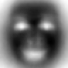
\includegraphics[interpolate=true,width=0.680000in,height=0.680000in]{weights-comparison-img0.png}}%
\end{pgfscope}%
\begin{pgfscope}%
\pgfpathrectangle{\pgfqpoint{0.881364in}{1.680588in}}{\pgfqpoint{0.679412in}{0.679412in}}%
\pgfusepath{clip}%
\pgfsys@transformshift{0.881364in}{1.680588in}%
\pgftext[left,bottom]{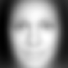
\includegraphics[interpolate=true,width=0.680000in,height=0.680000in]{weights-comparison-img1.png}}%
\end{pgfscope}%
\begin{pgfscope}%
\pgfpathrectangle{\pgfqpoint{0.050000in}{0.865294in}}{\pgfqpoint{0.679412in}{0.679412in}}%
\pgfusepath{clip}%
\pgfsys@transformshift{0.050000in}{0.865294in}%
\pgftext[left,bottom]{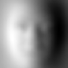
\includegraphics[interpolate=true,width=0.680000in,height=0.680000in]{weights-comparison-img2.png}}%
\end{pgfscope}%
\begin{pgfscope}%
\pgfpathrectangle{\pgfqpoint{0.881364in}{0.865294in}}{\pgfqpoint{0.679412in}{0.679412in}}%
\pgfusepath{clip}%
\pgfsys@transformshift{0.881364in}{0.865294in}%
\pgftext[left,bottom]{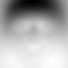
\includegraphics[interpolate=true,width=0.680000in,height=0.680000in]{weights-comparison-img3.png}}%
\end{pgfscope}%
\begin{pgfscope}%
\pgfpathrectangle{\pgfqpoint{0.050000in}{0.050000in}}{\pgfqpoint{0.679412in}{0.679412in}}%
\pgfusepath{clip}%
\pgfsys@transformshift{0.050000in}{0.050000in}%
\pgftext[left,bottom]{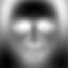
\includegraphics[interpolate=true,width=0.680000in,height=0.680000in]{weights-comparison-img4.png}}%
\end{pgfscope}%
\begin{pgfscope}%
\pgfpathrectangle{\pgfqpoint{0.881364in}{0.050000in}}{\pgfqpoint{0.679412in}{0.679412in}}%
\pgfusepath{clip}%
\pgfsys@transformshift{0.881364in}{0.050000in}%
\pgftext[left,bottom]{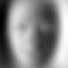
\includegraphics[interpolate=true,width=0.680000in,height=0.680000in]{weights-comparison-img5.png}}%
\end{pgfscope}%
\begin{pgfscope}%
\definecolor{textcolor}{rgb}{0.000000,0.000000,0.000000}%
\pgfsetstrokecolor{textcolor}%
\pgfsetfillcolor{textcolor}%
\pgftext[x=0.780804in,y=2.660000in,,top]{\color{textcolor}\rmfamily\fontsize{12.000000}{14.400000}\selectfont PCA}%
\end{pgfscope}%
\begin{pgfscope}%
\pgfsetbuttcap%
\pgfsetmiterjoin%
\definecolor{currentfill}{rgb}{1.000000,1.000000,1.000000}%
\pgfsetfillcolor{currentfill}%
\pgfsetlinewidth{0.000000pt}%
\definecolor{currentstroke}{rgb}{1.000000,1.000000,1.000000}%
\pgfsetstrokecolor{currentstroke}%
\pgfsetdash{}{0pt}%
\pgfpathmoveto{\pgfqpoint{1.764138in}{-0.280000in}}%
\pgfpathlineto{\pgfqpoint{3.730804in}{-0.280000in}}%
\pgfpathlineto{\pgfqpoint{3.730804in}{2.720000in}}%
\pgfpathlineto{\pgfqpoint{1.764138in}{2.720000in}}%
\pgfpathlineto{\pgfqpoint{1.764138in}{-0.280000in}}%
\pgfpathclose%
\pgfusepath{fill}%
\end{pgfscope}%
\begin{pgfscope}%
\pgfpathrectangle{\pgfqpoint{2.016667in}{1.680588in}}{\pgfqpoint{0.679412in}{0.679412in}}%
\pgfusepath{clip}%
\pgfsys@transformshift{2.016667in}{1.680588in}%
\pgftext[left,bottom]{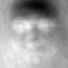
\includegraphics[interpolate=true,width=0.680000in,height=0.680000in]{weights-comparison-img6.png}}%
\end{pgfscope}%
\begin{pgfscope}%
\pgfpathrectangle{\pgfqpoint{2.848030in}{1.680588in}}{\pgfqpoint{0.679412in}{0.679412in}}%
\pgfusepath{clip}%
\pgfsys@transformshift{2.848030in}{1.680588in}%
\pgftext[left,bottom]{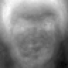
\includegraphics[interpolate=true,width=0.680000in,height=0.680000in]{weights-comparison-img7.png}}%
\end{pgfscope}%
\begin{pgfscope}%
\pgfpathrectangle{\pgfqpoint{2.016667in}{0.865294in}}{\pgfqpoint{0.679412in}{0.679412in}}%
\pgfusepath{clip}%
\pgfsys@transformshift{2.016667in}{0.865294in}%
\pgftext[left,bottom]{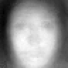
\includegraphics[interpolate=true,width=0.680000in,height=0.680000in]{weights-comparison-img8.png}}%
\end{pgfscope}%
\begin{pgfscope}%
\pgfpathrectangle{\pgfqpoint{2.848030in}{0.865294in}}{\pgfqpoint{0.679412in}{0.679412in}}%
\pgfusepath{clip}%
\pgfsys@transformshift{2.848030in}{0.865294in}%
\pgftext[left,bottom]{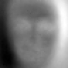
\includegraphics[interpolate=true,width=0.680000in,height=0.680000in]{weights-comparison-img9.png}}%
\end{pgfscope}%
\begin{pgfscope}%
\pgfpathrectangle{\pgfqpoint{2.016667in}{0.050000in}}{\pgfqpoint{0.679412in}{0.679412in}}%
\pgfusepath{clip}%
\pgfsys@transformshift{2.016667in}{0.050000in}%
\pgftext[left,bottom]{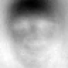
\includegraphics[interpolate=true,width=0.680000in,height=0.680000in]{weights-comparison-img10.png}}%
\end{pgfscope}%
\begin{pgfscope}%
\pgfpathrectangle{\pgfqpoint{2.848030in}{0.050000in}}{\pgfqpoint{0.679412in}{0.679412in}}%
\pgfusepath{clip}%
\pgfsys@transformshift{2.848030in}{0.050000in}%
\pgftext[left,bottom]{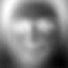
\includegraphics[interpolate=true,width=0.680000in,height=0.680000in]{weights-comparison-img11.png}}%
\end{pgfscope}%
\begin{pgfscope}%
\definecolor{textcolor}{rgb}{0.000000,0.000000,0.000000}%
\pgfsetstrokecolor{textcolor}%
\pgfsetfillcolor{textcolor}%
\pgftext[x=2.747471in,y=2.660000in,,top]{\color{textcolor}\rmfamily\fontsize{12.000000}{14.400000}\selectfont Linear AE}%
\end{pgfscope}%
\begin{pgfscope}%
\pgfsetbuttcap%
\pgfsetmiterjoin%
\definecolor{currentfill}{rgb}{1.000000,1.000000,1.000000}%
\pgfsetfillcolor{currentfill}%
\pgfsetlinewidth{0.000000pt}%
\definecolor{currentstroke}{rgb}{1.000000,1.000000,1.000000}%
\pgfsetstrokecolor{currentstroke}%
\pgfsetdash{}{0pt}%
\pgfpathmoveto{\pgfqpoint{3.730804in}{-0.280000in}}%
\pgfpathlineto{\pgfqpoint{5.697471in}{-0.280000in}}%
\pgfpathlineto{\pgfqpoint{5.697471in}{2.720000in}}%
\pgfpathlineto{\pgfqpoint{3.730804in}{2.720000in}}%
\pgfpathlineto{\pgfqpoint{3.730804in}{-0.280000in}}%
\pgfpathclose%
\pgfusepath{fill}%
\end{pgfscope}%
\begin{pgfscope}%
\pgfpathrectangle{\pgfqpoint{3.983333in}{1.680588in}}{\pgfqpoint{0.679412in}{0.679412in}}%
\pgfusepath{clip}%
\pgfsys@transformshift{3.983333in}{1.680588in}%
\pgftext[left,bottom]{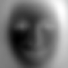
\includegraphics[interpolate=true,width=0.680000in,height=0.680000in]{weights-comparison-img12.png}}%
\end{pgfscope}%
\begin{pgfscope}%
\pgfpathrectangle{\pgfqpoint{4.814697in}{1.680588in}}{\pgfqpoint{0.679412in}{0.679412in}}%
\pgfusepath{clip}%
\pgfsys@transformshift{4.814697in}{1.680588in}%
\pgftext[left,bottom]{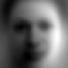
\includegraphics[interpolate=true,width=0.680000in,height=0.680000in]{weights-comparison-img13.png}}%
\end{pgfscope}%
\begin{pgfscope}%
\pgfpathrectangle{\pgfqpoint{3.983333in}{0.865294in}}{\pgfqpoint{0.679412in}{0.679412in}}%
\pgfusepath{clip}%
\pgfsys@transformshift{3.983333in}{0.865294in}%
\pgftext[left,bottom]{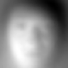
\includegraphics[interpolate=true,width=0.680000in,height=0.680000in]{weights-comparison-img14.png}}%
\end{pgfscope}%
\begin{pgfscope}%
\pgfpathrectangle{\pgfqpoint{4.814697in}{0.865294in}}{\pgfqpoint{0.679412in}{0.679412in}}%
\pgfusepath{clip}%
\pgfsys@transformshift{4.814697in}{0.865294in}%
\pgftext[left,bottom]{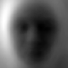
\includegraphics[interpolate=true,width=0.680000in,height=0.680000in]{weights-comparison-img15.png}}%
\end{pgfscope}%
\begin{pgfscope}%
\pgfpathrectangle{\pgfqpoint{3.983333in}{0.050000in}}{\pgfqpoint{0.679412in}{0.679412in}}%
\pgfusepath{clip}%
\pgfsys@transformshift{3.983333in}{0.050000in}%
\pgftext[left,bottom]{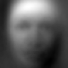
\includegraphics[interpolate=true,width=0.680000in,height=0.680000in]{weights-comparison-img16.png}}%
\end{pgfscope}%
\begin{pgfscope}%
\pgfpathrectangle{\pgfqpoint{4.814697in}{0.050000in}}{\pgfqpoint{0.679412in}{0.679412in}}%
\pgfusepath{clip}%
\pgfsys@transformshift{4.814697in}{0.050000in}%
\pgftext[left,bottom]{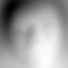
\includegraphics[interpolate=true,width=0.680000in,height=0.680000in]{weights-comparison-img17.png}}%
\end{pgfscope}%
\begin{pgfscope}%
\definecolor{textcolor}{rgb}{0.000000,0.000000,0.000000}%
\pgfsetstrokecolor{textcolor}%
\pgfsetfillcolor{textcolor}%
\pgftext[x=4.714138in,y=2.660000in,,top]{\color{textcolor}\rmfamily\fontsize{12.000000}{14.400000}\selectfont Sigmoid-linear AE}%
\end{pgfscope}%
\end{pgfpicture}%
\makeatother%
\endgroup%

	\caption[Die Gewichtsmatrizen von ausgewählten Methoden auf dem FER Datensatz]{Gezeigt sind die Gewichtsmatrizen von drei Methoden bei einer Reduktion des FER Datensatz auf sechs Dimensionen. Ein einzelnes Bild entspricht einer Spalte der Ladungs- beziehungsweise Gewichtsmatrix, welche in die Größe des Bildes umgeformt wurde. \captiona Die Ladungsmatrix $\mat{A}$ der Hauptkomponentenanalyse \captionb Die Decoder-Gewichtsmatrix eines linearen dreischichtigen Autoencoders \captionc Die Decoder-Gewichtsmatrix eines nichtlinearen dreischichtigen Autoencoders, wobei der Encoder eine Sigmoid-Aktivierungsfunktion einsetzt und der Decoder linear ist.
		Bei genauer Betrachtung der Ladungen von PCA und der Gewichte des linearen Autoencoders fällt auf, dass diese bis auf die Vorzeichen (erkennbar am invertierten Grauwert) fast identisch sind. Bei einem nichtlinearen Encoder ist dies nicht mehr der Fall. (Eigene Darstellung, angelehnt an \textcite[5]{Plaut.2018})}
	\label{fig:Gewichtsvergleich}
\end{figure}
Hierbei ist in \captiona die Ladungsmatrix von PCA, in \captionb die Gewichtsmatrix $\mat{W}_2$ eines linearen dreischichtigen Autoencoders und in \captionc die Gewichtsmatrix $\mat{W}_2$ eines nichtlinearen Autoencoders dargestellt. Wie zu erkennen ist, sind
die Gewichte des linearen Autoencoders bis auf das Vorzeichen sehr ähnlich zur Ladungsmatrix von
PCA.